% Inherit from report

% Default to the notebook output style

    


% Inherit from the specified cell style.




    
\documentclass{book}
\setcounter{chapter}{0}
\usepackage{pmboxdraw}
\usepackage{verbatim}
\usepackage{listings}


\lstset{
language={}, 
basicstyle=\ttfamily,
xleftmargin=4ex,
stringstyle=\color{cm-string},
commentstyle=\color{cm-comment},
keywordstyle=\color{cm-keyword}\bfseries,
%keywordstyle = {[3]\color{cm-operator}},
%morekeywords = [3]{>>>,+,-,/,*,**,%},
showstringspaces=false,
}
\newcommand{\passthrough}[1]{#1}

    
    
    \usepackage[T1]{fontenc}
    % Nicer default font (+ math font) than Computer Modern for most use cases
    \setlength{\parskip}{0.5em} %for a space between paragraphs that is not a full space
    \setlength{\parindent}{0em} %for no indentation between paragraphs
    \usepackage{mathpazo}

    % Basic figure setup, for now with no caption control since it's done
    % automatically by Pandoc (which extracts ![](path) syntax from Markdown).
    \usepackage{graphicx}
    % We will generate all images so they have a width \maxwidth. This means
    % that they will get their normal width if they fit onto the page, but
    % are scaled down if they would overflow the margins.
    \makeatletter
    \def\maxwidth{\ifdim\Gin@nat@width>\linewidth\linewidth
    \else\Gin@nat@width\fi}
    \makeatother
    \let\Oldincludegraphics\includegraphics
    % Set max figure width to be 80% of text width, for now hardcoded.
    \renewcommand{\includegraphics}[1]{\Oldincludegraphics[width=.8\maxwidth]{#1}}
    % Ensure that by default, figures have no caption (until we provide a
    % proper Figure object with a Caption API and a way to capture that
    % in the conversion process - todo).
    \usepackage{caption}
    \DeclareCaptionLabelFormat{nolabel}{}
    \captionsetup{labelformat=nolabel}

    \usepackage{adjustbox} % Used to constrain images to a maximum size
    \usepackage{xcolor} % Allow colors to be defined

%custom colors
\definecolor{stringred}{RGB}{186,33,33}
\definecolor{commentteal}{RGB}{64,128,128}
\definecolor{darkgreen}{RGB}{0,128,0}
\definecolor{cm-keyword}{HTML}{008000}  %jupyter notebook keyword color
\definecolor{cm-builtin}{HTML}{008000}  %jupyter notebook built-in function color
\definecolor{cm-number}{HTML}{008800}   %jupyter notebook number color
\definecolor{cm-string}{HTML}{BA2121}   %jupyter notebook string color
\definecolor{cm-operator}{HTML}{AA22FF} %jupyter notebook operator color
\definecolor{cm-comment}{HTML}{408080}  %jupyter notebook comment color




    \usepackage{enumerate} % Needed for markdown enumerations to work
    \usepackage{geometry} % Used to adjust the document margins
    \geometry{
        verbose,
        papersize={8in,10in},
        tmargin=1in,
        bmargin=0.75in,
        lmargin=1.0in,
        rmargin=1.0in}
    \usepackage{amsmath} % Equations
    \usepackage{amssymb} % Equations
    \usepackage{textcomp} % defines textquotesingle
    % Hack from http://tex.stackexchange.com/a/47451/13684:
    \AtBeginDocument{%
        \def\PYZsq{\textquotesingle}% Upright quotes in Pygmentized code
    }
    \usepackage{upquote} % Upright quotes for verbatim code
    \usepackage{eurosym} % defines \euro
    \usepackage[mathletters]{ucs} % Extended unicode (utf-8) support
    \usepackage[utf8x]{inputenc} % Allow utf-8 characters in the tex document
    \usepackage{fancyvrb} % verbatim replacement that allows latex
    \usepackage{grffile} % extends the file name processing of package graphics
                         % to support a larger range
    % The hyperref package gives us a pdf with properly built
    % internal navigation ('pdf bookmarks' for the table of contents,
    % internal cross-reference links, web links for URLs, etc.)
    \usepackage{hyperref}
    \usepackage{longtable} % longtable support required by pandoc >1.10
    \usepackage{booktabs}  % table support for pandoc > 1.12.2
    \usepackage[inline]{enumitem} % IRkernel/repr support (it uses the enumerate* environment)
    \usepackage[normalem]{ulem} % ulem is needed to support strikethroughs (\sout)
                                % normalem makes italics be italics, not underlines
    \usepackage{titlesec}
    \setcounter{secnumdepth}{1} %only chapter and sections are numbered, subsections and subsubsections are not numbered
    \setcounter{tocdepth}{1}    %only chapter and sections in TOC, subsections and subsubsections are not in TOC
    \usepackage{multicol} % need multicols for end of chapter key terms and end of chapter questions

    \newenvironment{problems}{}{}  %keep regular one column formatting in problems environment. Long table would not output in two col mode
%    \newenvironment{problems}{\begin{multicols}{2}}{\end{multicols}} %an environment for the review question sections, where two columns are shown instead of one column everywhere else. Depends on the logic looking for latex environment problems in notebook cell metadata.

% in cell metadata
%{
%  "latex": {
%    "environment": "problems"
%  }
%}


    \newenvironment{key_terms}{\begin{multicols}{3}}{\end{multicols}} %an environment for the key_terms and concepts sections, where three columns are shown instead of one column everywhere else. Depends on the logic looking for latex environment key terms in notebook cell metadata.

% in cell metadata
%{
%  "latex": {
%    "environment": "key_terms"
%  }
%}

% to put a \new page before the cell in question. Add the json below to the cell metadata.

% in cell metadata
%{
%  "latex": {
%    "before_cell": "newpage"
%  }
%}


% to put a \newpage after the cell in question. Add the json below to the cell metadata.
% in cell metadata
%{
%  "latex": {
%    "after_cell": "newpage"
%  }
%}

    

    
    
    % Colors for the hyperref package
    \definecolor{urlcolor}{rgb}{0,.145,.698}
    \definecolor{linkcolor}{rgb}{.71,0.21,0.01}
    \definecolor{citecolor}{rgb}{.12,.54,.11}

    % ANSI colors
    \definecolor{ansi-black}{HTML}{3E424D}
    \definecolor{ansi-black-intense}{HTML}{282C36}
    \definecolor{ansi-red}{HTML}{E75C58}
    \definecolor{ansi-red-intense}{HTML}{B22B31}
    \definecolor{ansi-green}{HTML}{00A250}
    \definecolor{ansi-green-intense}{HTML}{007427}
    \definecolor{ansi-yellow}{HTML}{DDB62B}
    \definecolor{ansi-yellow-intense}{HTML}{B27D12}
    \definecolor{ansi-blue}{HTML}{208FFB}
    \definecolor{ansi-blue-intense}{HTML}{0065CA}
    \definecolor{ansi-magenta}{HTML}{D160C4}
    \definecolor{ansi-magenta-intense}{HTML}{A03196}
    \definecolor{ansi-cyan}{HTML}{60C6C8}
    \definecolor{ansi-cyan-intense}{HTML}{258F8F}
    \definecolor{ansi-white}{HTML}{C5C1B4}
    \definecolor{ansi-white-intense}{HTML}{A1A6B2}
    \definecolor{ansi-default-inverse-fg}{HTML}{FFFFFF}
    \definecolor{ansi-default-inverse-bg}{HTML}{000000}

    % commands and environments needed by pandoc snippets
    % extracted from the output of `pandoc -s`
    \providecommand{\tightlist}{%
      \setlength{\itemsep}{0pt}\setlength{\parskip}{0pt}}
    \DefineVerbatimEnvironment{Highlighting}{Verbatim}{commandchars=\\\{\}}
    % Add ',fontsize=\small' for more characters per line
    \newenvironment{Shaded}{}{}
    \newcommand{\KeywordTok}[1]{\textcolor[rgb]{0.00,0.44,0.13}{\textbf{{#1}}}}
    \newcommand{\DataTypeTok}[1]{\textcolor[rgb]{0.56,0.13,0.00}{{#1}}}
    \newcommand{\DecValTok}[1]{\textcolor[rgb]{0.25,0.63,0.44}{{#1}}}
    \newcommand{\BaseNTok}[1]{\textcolor[rgb]{0.25,0.63,0.44}{{#1}}}
    \newcommand{\FloatTok}[1]{\textcolor[rgb]{0.25,0.63,0.44}{{#1}}}
    \newcommand{\CharTok}[1]{\textcolor[rgb]{0.25,0.44,0.63}{{#1}}}
    \newcommand{\StringTok}[1]{\textcolor[rgb]{0.25,0.44,0.63}{{#1}}}
    \newcommand{\CommentTok}[1]{\textcolor[rgb]{0.38,0.63,0.69}{\textit{{#1}}}}
    \newcommand{\OtherTok}[1]{\textcolor[rgb]{0.00,0.44,0.13}{{#1}}}
    \newcommand{\AlertTok}[1]{\textcolor[rgb]{1.00,0.00,0.00}{\textbf{{#1}}}}
    \newcommand{\FunctionTok}[1]{\textcolor[rgb]{0.02,0.16,0.49}{{#1}}}
    \newcommand{\RegionMarkerTok}[1]{{#1}}
    \newcommand{\ErrorTok}[1]{\textcolor[rgb]{1.00,0.00,0.00}{\textbf{{#1}}}}
    \newcommand{\NormalTok}[1]{{#1}}
    
    % Additional commands for more recent versions of Pandoc
    \newcommand{\ConstantTok}[1]{\textcolor[rgb]{0.53,0.00,0.00}{{#1}}}
    \newcommand{\SpecialCharTok}[1]{\textcolor[rgb]{0.25,0.44,0.63}{{#1}}}
    \newcommand{\VerbatimStringTok}[1]{\textcolor[rgb]{0.25,0.44,0.63}{{#1}}}
    \newcommand{\SpecialStringTok}[1]{\textcolor[rgb]{0.73,0.40,0.53}{{#1}}}
    \newcommand{\ImportTok}[1]{{#1}}
    \newcommand{\DocumentationTok}[1]{\textcolor[rgb]{0.73,0.13,0.13}{\textit{{#1}}}}
    \newcommand{\AnnotationTok}[1]{\textcolor[rgb]{0.38,0.63,0.69}{\textbf{\textit{{#1}}}}}
    \newcommand{\CommentVarTok}[1]{\textcolor[rgb]{0.38,0.63,0.69}{\textbf{\textit{{#1}}}}}
    \newcommand{\VariableTok}[1]{\textcolor[rgb]{0.10,0.09,0.49}{{#1}}}
    \newcommand{\ControlFlowTok}[1]{\textcolor[rgb]{0.00,0.44,0.13}{\textbf{{#1}}}}
    \newcommand{\OperatorTok}[1]{\textcolor[rgb]{0.40,0.40,0.40}{{#1}}}
    \newcommand{\BuiltInTok}[1]{{#1}}
    \newcommand{\ExtensionTok}[1]{{#1}}
    \newcommand{\PreprocessorTok}[1]{\textcolor[rgb]{0.74,0.48,0.00}{{#1}}}
    \newcommand{\AttributeTok}[1]{\textcolor[rgb]{0.49,0.56,0.16}{{#1}}}
    \newcommand{\InformationTok}[1]{\textcolor[rgb]{0.38,0.63,0.69}{\textbf{\textit{{#1}}}}}
    \newcommand{\WarningTok}[1]{\textcolor[rgb]{0.38,0.63,0.69}{\textbf{\textit{{#1}}}}}
    
    
    % Define a nice break command that doesn't care if a line doesn't already
    % exist.
    \def\br{\hspace*{\fill} \\* }
    % Math Jax compatibility definitions
    \def\gt{>}
    \def\lt{<}
    \let\Oldtex\TeX
    \let\Oldlatex\LaTeX
    \renewcommand{\TeX}{\textrm{\Oldtex}}
    \renewcommand{\LaTeX}{\textrm{\Oldlatex}}
    % Document parameters
    % Document title
    
\title{Problem Solving with Python}
\author{Peter D. Kazarinoff, PhD}
\date{}

    
    
    
    
    

    % Pygments definitions
    
\makeatletter
\def\PY@reset{\let\PY@it=\relax \let\PY@bf=\relax%
    \let\PY@ul=\relax \let\PY@tc=\relax%
    \let\PY@bc=\relax \let\PY@ff=\relax}
\def\PY@tok#1{\csname PY@tok@#1\endcsname}
\def\PY@toks#1+{\ifx\relax#1\empty\else%
    \PY@tok{#1}\expandafter\PY@toks\fi}
\def\PY@do#1{\PY@bc{\PY@tc{\PY@ul{%
    \PY@it{\PY@bf{\PY@ff{#1}}}}}}}
\def\PY#1#2{\PY@reset\PY@toks#1+\relax+\PY@do{#2}}

\expandafter\def\csname PY@tok@w\endcsname{\def\PY@tc##1{\textcolor[rgb]{0.73,0.73,0.73}{##1}}}
\expandafter\def\csname PY@tok@c\endcsname{\let\PY@it=\textit\def\PY@tc##1{\textcolor[rgb]{0.25,0.50,0.50}{##1}}}
\expandafter\def\csname PY@tok@cp\endcsname{\def\PY@tc##1{\textcolor[rgb]{0.74,0.48,0.00}{##1}}}
\expandafter\def\csname PY@tok@k\endcsname{\let\PY@bf=\textbf\def\PY@tc##1{\textcolor[rgb]{0.00,0.50,0.00}{##1}}}
\expandafter\def\csname PY@tok@kp\endcsname{\def\PY@tc##1{\textcolor[rgb]{0.00,0.50,0.00}{##1}}}
\expandafter\def\csname PY@tok@kt\endcsname{\def\PY@tc##1{\textcolor[rgb]{0.69,0.00,0.25}{##1}}}
\expandafter\def\csname PY@tok@o\endcsname{\def\PY@tc##1{\textcolor[rgb]{0.40,0.40,0.40}{##1}}}
\expandafter\def\csname PY@tok@ow\endcsname{\let\PY@bf=\textbf\def\PY@tc##1{\textcolor[rgb]{0.67,0.13,1.00}{##1}}}
\expandafter\def\csname PY@tok@nb\endcsname{\def\PY@tc##1{\textcolor[rgb]{0.00,0.50,0.00}{##1}}}
\expandafter\def\csname PY@tok@nf\endcsname{\def\PY@tc##1{\textcolor[rgb]{0.00,0.00,1.00}{##1}}}
\expandafter\def\csname PY@tok@nc\endcsname{\let\PY@bf=\textbf\def\PY@tc##1{\textcolor[rgb]{0.00,0.00,1.00}{##1}}}
\expandafter\def\csname PY@tok@nn\endcsname{\let\PY@bf=\textbf\def\PY@tc##1{\textcolor[rgb]{0.00,0.00,1.00}{##1}}}
\expandafter\def\csname PY@tok@ne\endcsname{\let\PY@bf=\textbf\def\PY@tc##1{\textcolor[rgb]{0.82,0.25,0.23}{##1}}}
\expandafter\def\csname PY@tok@nv\endcsname{\def\PY@tc##1{\textcolor[rgb]{0.10,0.09,0.49}{##1}}}
\expandafter\def\csname PY@tok@no\endcsname{\def\PY@tc##1{\textcolor[rgb]{0.53,0.00,0.00}{##1}}}
\expandafter\def\csname PY@tok@nl\endcsname{\def\PY@tc##1{\textcolor[rgb]{0.63,0.63,0.00}{##1}}}
\expandafter\def\csname PY@tok@ni\endcsname{\let\PY@bf=\textbf\def\PY@tc##1{\textcolor[rgb]{0.60,0.60,0.60}{##1}}}
\expandafter\def\csname PY@tok@na\endcsname{\def\PY@tc##1{\textcolor[rgb]{0.49,0.56,0.16}{##1}}}
\expandafter\def\csname PY@tok@nt\endcsname{\let\PY@bf=\textbf\def\PY@tc##1{\textcolor[rgb]{0.00,0.50,0.00}{##1}}}
\expandafter\def\csname PY@tok@nd\endcsname{\def\PY@tc##1{\textcolor[rgb]{0.67,0.13,1.00}{##1}}}
\expandafter\def\csname PY@tok@s\endcsname{\def\PY@tc##1{\textcolor[rgb]{0.73,0.13,0.13}{##1}}}
\expandafter\def\csname PY@tok@sd\endcsname{\let\PY@it=\textit\def\PY@tc##1{\textcolor[rgb]{0.73,0.13,0.13}{##1}}}
\expandafter\def\csname PY@tok@si\endcsname{\let\PY@bf=\textbf\def\PY@tc##1{\textcolor[rgb]{0.73,0.40,0.53}{##1}}}
\expandafter\def\csname PY@tok@se\endcsname{\let\PY@bf=\textbf\def\PY@tc##1{\textcolor[rgb]{0.73,0.40,0.13}{##1}}}
\expandafter\def\csname PY@tok@sr\endcsname{\def\PY@tc##1{\textcolor[rgb]{0.73,0.40,0.53}{##1}}}
\expandafter\def\csname PY@tok@ss\endcsname{\def\PY@tc##1{\textcolor[rgb]{0.10,0.09,0.49}{##1}}}
\expandafter\def\csname PY@tok@sx\endcsname{\def\PY@tc##1{\textcolor[rgb]{0.00,0.50,0.00}{##1}}}
\expandafter\def\csname PY@tok@m\endcsname{\def\PY@tc##1{\textcolor[rgb]{0.40,0.40,0.40}{##1}}}
\expandafter\def\csname PY@tok@gh\endcsname{\let\PY@bf=\textbf\def\PY@tc##1{\textcolor[rgb]{0.00,0.00,0.50}{##1}}}
\expandafter\def\csname PY@tok@gu\endcsname{\let\PY@bf=\textbf\def\PY@tc##1{\textcolor[rgb]{0.50,0.00,0.50}{##1}}}
\expandafter\def\csname PY@tok@gd\endcsname{\def\PY@tc##1{\textcolor[rgb]{0.63,0.00,0.00}{##1}}}
\expandafter\def\csname PY@tok@gi\endcsname{\def\PY@tc##1{\textcolor[rgb]{0.00,0.63,0.00}{##1}}}
\expandafter\def\csname PY@tok@gr\endcsname{\def\PY@tc##1{\textcolor[rgb]{1.00,0.00,0.00}{##1}}}
\expandafter\def\csname PY@tok@ge\endcsname{\let\PY@it=\textit}
\expandafter\def\csname PY@tok@gs\endcsname{\let\PY@bf=\textbf}
\expandafter\def\csname PY@tok@gp\endcsname{\let\PY@bf=\textbf\def\PY@tc##1{\textcolor[rgb]{0.00,0.00,0.50}{##1}}}
\expandafter\def\csname PY@tok@go\endcsname{\def\PY@tc##1{\textcolor[rgb]{0.53,0.53,0.53}{##1}}}
\expandafter\def\csname PY@tok@gt\endcsname{\def\PY@tc##1{\textcolor[rgb]{0.00,0.27,0.87}{##1}}}
\expandafter\def\csname PY@tok@err\endcsname{\def\PY@bc##1{\setlength{\fboxsep}{0pt}\fcolorbox[rgb]{1.00,0.00,0.00}{1,1,1}{\strut ##1}}}
\expandafter\def\csname PY@tok@kc\endcsname{\let\PY@bf=\textbf\def\PY@tc##1{\textcolor[rgb]{0.00,0.50,0.00}{##1}}}
\expandafter\def\csname PY@tok@kd\endcsname{\let\PY@bf=\textbf\def\PY@tc##1{\textcolor[rgb]{0.00,0.50,0.00}{##1}}}
\expandafter\def\csname PY@tok@kn\endcsname{\let\PY@bf=\textbf\def\PY@tc##1{\textcolor[rgb]{0.00,0.50,0.00}{##1}}}
\expandafter\def\csname PY@tok@kr\endcsname{\let\PY@bf=\textbf\def\PY@tc##1{\textcolor[rgb]{0.00,0.50,0.00}{##1}}}
\expandafter\def\csname PY@tok@bp\endcsname{\def\PY@tc##1{\textcolor[rgb]{0.00,0.50,0.00}{##1}}}
\expandafter\def\csname PY@tok@fm\endcsname{\def\PY@tc##1{\textcolor[rgb]{0.00,0.00,1.00}{##1}}}
\expandafter\def\csname PY@tok@vc\endcsname{\def\PY@tc##1{\textcolor[rgb]{0.10,0.09,0.49}{##1}}}
\expandafter\def\csname PY@tok@vg\endcsname{\def\PY@tc##1{\textcolor[rgb]{0.10,0.09,0.49}{##1}}}
\expandafter\def\csname PY@tok@vi\endcsname{\def\PY@tc##1{\textcolor[rgb]{0.10,0.09,0.49}{##1}}}
\expandafter\def\csname PY@tok@vm\endcsname{\def\PY@tc##1{\textcolor[rgb]{0.10,0.09,0.49}{##1}}}
\expandafter\def\csname PY@tok@sa\endcsname{\def\PY@tc##1{\textcolor[rgb]{0.73,0.13,0.13}{##1}}}
\expandafter\def\csname PY@tok@sb\endcsname{\def\PY@tc##1{\textcolor[rgb]{0.73,0.13,0.13}{##1}}}
\expandafter\def\csname PY@tok@sc\endcsname{\def\PY@tc##1{\textcolor[rgb]{0.73,0.13,0.13}{##1}}}
\expandafter\def\csname PY@tok@dl\endcsname{\def\PY@tc##1{\textcolor[rgb]{0.73,0.13,0.13}{##1}}}
\expandafter\def\csname PY@tok@s2\endcsname{\def\PY@tc##1{\textcolor[rgb]{0.73,0.13,0.13}{##1}}}
\expandafter\def\csname PY@tok@sh\endcsname{\def\PY@tc##1{\textcolor[rgb]{0.73,0.13,0.13}{##1}}}
\expandafter\def\csname PY@tok@s1\endcsname{\def\PY@tc##1{\textcolor[rgb]{0.73,0.13,0.13}{##1}}}
\expandafter\def\csname PY@tok@mb\endcsname{\def\PY@tc##1{\textcolor[rgb]{0.40,0.40,0.40}{##1}}}
\expandafter\def\csname PY@tok@mf\endcsname{\def\PY@tc##1{\textcolor[rgb]{0.40,0.40,0.40}{##1}}}
\expandafter\def\csname PY@tok@mh\endcsname{\def\PY@tc##1{\textcolor[rgb]{0.40,0.40,0.40}{##1}}}
\expandafter\def\csname PY@tok@mi\endcsname{\def\PY@tc##1{\textcolor[rgb]{0.40,0.40,0.40}{##1}}}
\expandafter\def\csname PY@tok@il\endcsname{\def\PY@tc##1{\textcolor[rgb]{0.40,0.40,0.40}{##1}}}
\expandafter\def\csname PY@tok@mo\endcsname{\def\PY@tc##1{\textcolor[rgb]{0.40,0.40,0.40}{##1}}}
\expandafter\def\csname PY@tok@ch\endcsname{\let\PY@it=\textit\def\PY@tc##1{\textcolor[rgb]{0.25,0.50,0.50}{##1}}}
\expandafter\def\csname PY@tok@cm\endcsname{\let\PY@it=\textit\def\PY@tc##1{\textcolor[rgb]{0.25,0.50,0.50}{##1}}}
\expandafter\def\csname PY@tok@cpf\endcsname{\let\PY@it=\textit\def\PY@tc##1{\textcolor[rgb]{0.25,0.50,0.50}{##1}}}
\expandafter\def\csname PY@tok@c1\endcsname{\let\PY@it=\textit\def\PY@tc##1{\textcolor[rgb]{0.25,0.50,0.50}{##1}}}
\expandafter\def\csname PY@tok@cs\endcsname{\let\PY@it=\textit\def\PY@tc##1{\textcolor[rgb]{0.25,0.50,0.50}{##1}}}

\def\PYZbs{\char`\\}
\def\PYZus{\char`\_}
\def\PYZob{\char`\{}
\def\PYZcb{\char`\}}
\def\PYZca{\char`\^}
\def\PYZam{\char`\&}
\def\PYZlt{\char`\<}
\def\PYZgt{\char`\>}
\def\PYZsh{\char`\#}
\def\PYZpc{\char`\%}
\def\PYZdl{\char`\$}
\def\PYZhy{\char`\-}
\def\PYZsq{\char`\'}
\def\PYZdq{\char`\"}
\def\PYZti{\char`\~}
% for compatibility with earlier versions
\def\PYZat{@}
\def\PYZlb{[}
\def\PYZrb{]}
\makeatother


    % Exact colors from NB
    \definecolor{incolor}{rgb}{0.0, 0.0, 0.5}
    \definecolor{outcolor}{rgb}{0.545, 0.0, 0.0}



    
    % Prevent overflowing lines due to hard-to-break entities
    \sloppy 
    % Setup hyperref package
    \hypersetup{
      breaklinks=true,  % so long urls are correctly broken across lines
      colorlinks=true,
      urlcolor=urlcolor,
      linkcolor=linkcolor,
      citecolor=citecolor,
      }
    % Slightly bigger margins than the latex defaults
    

    

    \begin{document}
    
    
    
    \maketitle
    
    
    \tableofcontents


    

    
        \hypertarget{preface}{%
\chapter{Preface}\label{preface}}
    




    
        \hypertarget{motivation}{%
\section{Motivation}\label{motivation}}
    




    
        The motivation for writing this book is that many undergraduate
engineering students have to take a programming course based on MATLAB.
MATLAB is a great piece of software, but it currently costs \$49.00 for
a student license and requires a site license to be used on school
computers. Subsequently, it is costly for a student to use MATLAB and it
is costly for a college to support a course that uses MATLAB. In
addition, this site license expires eventually and students need to
purchase another copy often before they finish their degree.

The Python programming language, on the other hand, is open source and
free. To download and use Python, the cost to both the student and the
college is zero (minus time spent). By moving an undergraduate
engineering programming class to Python, students will save money and
have greater access to the software they use in class. Further in their
engineering education, students can continue to use Python for free.
    



    \begin{Verbatim}[commandchars=\\\{\}]
{\color{incolor}In [{\color{incolor} }]:} 
\end{Verbatim}


    
        \hypertarget{acknowledgments}{%
\section{Acknowledgments}\label{acknowledgments}}
    




    
        The creation of this book and supporting material would not be possible
without the gracious support of my wife and family. Students at Portland
Community College continue to give me hope that the next generation of
engineers will be a diverse group of team problem solvers.

\emph{The Python Data Science Handbook} and \emph{Machine Learning in
Python} as well as \emph{Reiman Equations in Python} served as
inspiration and examples of using Jupyter notebooks to construct a book.
The \emph{bookbook} repository on GitHub provided a starting point for
the tooling used to convert this book from Jupyter notebooks into a
website and into LaTeX for printing.
    



    \begin{Verbatim}[commandchars=\\\{\}]
{\color{incolor}In [{\color{incolor} }]:} 
\end{Verbatim}


    
        \hypertarget{supporting-materials}{%
\section{Supporting Materials}\label{supporting-materials}}
    




    
        Supporting materials for this text can be found on the textbook website:

\begin{quote}
\url{https://problemsolvingwithpython.com}
\end{quote}

The textbook website contains all of the text in web format. Code
examples and Jupyter notebooks for the text can be found in the GitHub
repository for the book:

\begin{quote}
\url{https:github.com/ProfessorKazarinoff/Problem-Solving-with-Python}
\end{quote}

Live notebooks, where code examples found in the text can be run without
installing any software, are available at:

\begin{quote}
\url{https://mybinder.org/v2/gh/ProfessorKazarinoff/Problem-Solving-with-Python/master}
\end{quote}

If you are an instructor and using this book in a course with students-
please send me an email using your school email address. In the email,
include the course you are teaching and the term, approximate
enrollment, and a link to the course listing on your school website.

\begin{quote}
peter.kazarinoff@problemsolvingwithpython.com
\end{quote}

I am happy to reply with a solution key for the end of chapter review
problems as well as quiz and exam question banks.
    



    \begin{Verbatim}[commandchars=\\\{\}]
{\color{incolor}In [{\color{incolor} }]:} 
\end{Verbatim}


    
        \hypertarget{formatting-conventions}{%
\section{Formatting Conventions}\label{formatting-conventions}}
    




    
        This book and supporting materials use the following formatting
conventions:
    




    
        \hypertarget{web-address}{%
\subsection{Web Address}\label{web-address}}

Web address will be shown as:

\begin{quote}
\url{https://github.com/professorkazarinoff/Problem-Solving-with-Python}
\end{quote}
    




    
        \hypertarget{import-terms-and-vocabulary}{%
\subsection{Import terms and
vocabulary}\label{import-terms-and-vocabulary}}

Important terms and vocabulary are shown in \emph{italic text}

\begin{quote}
There is a difference between \emph{local variables} and \emph{global
variables} in Python code.
\end{quote}
    




    
        \hypertarget{file-names}{%
\subsection{File Names}\label{file-names}}

File Names are shown in \textbf{\emph{bold and italic text}}

\begin{quote}
After completing the code, save the file as \textbf{\emph{hello.py}} in
the current directory.
\end{quote}
    




    
        \hypertarget{module-and-package-names}{%
\subsection{Module and Package Names}\label{module-and-package-names}}

Module and Package names will be shown in \textbf{bold text}

\begin{quote}
\textbf{NumPy} and \textbf{Matplotlib} are two useful packages for
problem solvers.
\end{quote}
    




    
        \hypertarget{inline-code}{%
\subsection{Inline code}\label{inline-code}}

Inline code, including variable names, is shown in
\passthrough{\lstinline!monospace font!}

\begin{quote}
To compare a variable use \passthrough{\lstinline!var == 'string'!} and
make sure to include \passthrough{\lstinline!==!}, the double equals
sign.
\end{quote}
    




    
        \hypertarget{separate-code-blocks}{%
\subsection{Separate code blocks}\label{separate-code-blocks}}

Separate code blocks appear in their own sections in
\passthrough{\lstinline!monospaced font!}

\begin{lstlisting}[language=Python]
import numpy as np
import pandas as pd
import matplotlib.pyplot as plt
\end{lstlisting}
    




    
        \hypertarget{anaconda-prompt-commands}{%
\subsection{Anaconda Prompt Commands}\label{anaconda-prompt-commands}}

Commands typed into the \textbf{Anaconda Prompt} are shown in separate
sections which contain the prompt symbol \passthrough{\lstinline!>!}
before each line. Note the prompt \passthrough{\lstinline!>!} should not
be typed. The prompt symbol is included to indicate \textbf{Anaconda
Prompt}, not a character for the user to enter.

\begin{lstlisting}
> conda create -n env python=3.7
> conda activate env
\end{lstlisting}
    




    
        \hypertarget{terminal-commands}{%
\subsection{Terminal Commands}\label{terminal-commands}}

Commands typed into the MacOS or Linux terminal appear in separate
sections which contain the dollar symbol \passthrough{\lstinline!$!}
before each line. Note the dollar symbol \passthrough{\lstinline!$!}
should not be typed. The dollar symbol is included to indicate a
terminal prompt, not a character for the user to enter.

\begin{lstlisting}
$ pip install pint
$ cd pint_srcipts
\end{lstlisting}
    




    
        \hypertarget{python-repl-commands}{%
\subsection{Python REPL Commands}\label{python-repl-commands}}

Commands typed into the \textbf{Python REPL} (the Python Interpreter)
appears in separate code sections, which contain the triple arrow prompt
\passthrough{\lstinline!>>>!} . Note the triple arrow
\passthrough{\lstinline!>>>!} prompt should not be typed. Triple arrows
are included to indicate the Python REPL prompt, not a character for the
user to enter. The output from the Python REPL is shown on a separate
line below the command, without the \passthrough{\lstinline!>>>!}
prompt.

\begin{lstlisting}[language=Python]
>>> 2 + 2
4
>>> print('Problem Solving with Python')
Problem Solving with Python
\end{lstlisting}
    




    
        \hypertarget{jupyter-notebook-cells}{%
\subsection{Jupyter Notebook cells}\label{jupyter-notebook-cells}}

Commands typed into Jupyter notebook cells appear with the label
\passthrough{\lstinline!In [#]:!} to the left of the code section. The
output from Jupyter notebook cells is shown below the input cell. Only
code in the input cells needs to be typed. Output cell are be produced
automatically by clicking the run button or typing
\passthrough{\lstinline![shift]+[Enter]!}
    



    \begin{Verbatim}[commandchars=\\\{\}]
{\color{incolor}In [{\color{incolor}1}]:} \PY{n}{A} \PY{o}{=} \PY{l+m+mi}{2}
        \PY{n}{B} \PY{o}{=} \PY{l+m+mi}{3}
        \PY{n}{C} \PY{o}{=} \PY{n}{A} \PY{o}{+} \PY{n}{B}
        \PY{n+nb}{print}\PY{p}{(}\PY{n}{C}\PY{p}{)}
\end{Verbatim}

    \begin{Verbatim}[commandchars=\\\{\}]
5

    \end{Verbatim}


    
        \hypertarget{keystrokes-and-buttons}{%
\subsection{Keystrokes and Buttons}\label{keystrokes-and-buttons}}

Keystrokes directly entered by the keyboard or buttons that are
indicated on programs or web pages are shown inside square brackets in
\passthrough{\lstinline![monospaced font]!}.

\begin{quote}
In order to delete a line use the \passthrough{\lstinline![Backspace]!}
key. To exit the shell type \passthrough{\lstinline![shift]+[c]!}
\end{quote}
    



    \begin{Verbatim}[commandchars=\\\{\}]
{\color{incolor}In [{\color{incolor} }]:} 
\end{Verbatim}


    
        \hypertarget{errata}{%
\section{Errata}\label{errata}}
    




    
        Errata including any typos, code errors and formatting inconsistencies
can be submitted to:

\begin{quote}
errata@problemsolvingwithpython.com
\end{quote}

Please include the chapter number and section number in your email.
Thank-you in advance for helping improve this text for future readers.
    



    \begin{Verbatim}[commandchars=\\\{\}]
{\color{incolor}In [{\color{incolor} }]:} 
\end{Verbatim}


    
        \hypertarget{orientation}{%
\chapter{Orientation}\label{orientation}}
    




    
        \hypertarget{introduction}{%
\section{Introduction}\label{introduction}}
    




    
        Welcome to the world of problem-solving with Python. This first
Orientation Chapter will help you get started by guiding you through the
process of installing Python on your computer.
    




    
        \hypertarget{by-the-end-of-this-chapter-you-will-be-able-to}{%
\subsection{By the end of this chapter, you will be able
to:}\label{by-the-end-of-this-chapter-you-will-be-able-to}}

\begin{itemize}
\item
  Describe why Python is a good programming language for problem solvers
\item
  Describe applications where Python is used
\item
  Detail advantages of Python over other programming languages
\item
  Know the cost of Python
\item
  Know the difference between Python and Anaconda
\item
  Install Python on your computer
\item
  Install Anaconda on your computer
\end{itemize}
        \newpage



    



    \begin{Verbatim}[commandchars=\\\{\}]
{\color{incolor}In [{\color{incolor} }]:} 
\end{Verbatim}


    
        \hypertarget{why-python}{%
\section{Why Python?}\label{why-python}}
    




    
        You might be wondering ``Why should I solve problems with Python?''
There are other programming languages in the world such as MATLAB,
LabView, C++ and Java. What makes Python useful for solving problems?
    




    
        \hypertarget{python-is-a-powerful-programming-language}{%
\subsection{Python is a powerful programming
language}\label{python-is-a-powerful-programming-language}}

Python defines the types of objects you build into your code. Unlike
some other languages such as C, you do not need to declare the object
type. The object type is also mutable, you can change the type of object
easily and on the fly. There is a wide array of object types built into
Python. Objects can change in size. Python objects can also contain
mixed data types. Strings and floating point numbers can be part of the
same list.

Python has an extensive Standard Library. A huge number of object types,
functions and methods are available for use without importing any
external modules. These include math functions, list methods, and calls
to a computer's system. There is a lot that can be done with the Python
Standard Library. The first couple of chapters of this book will just
use the standard library. It can do a lot.

Python has over 100,000 external packages available for download and
use. They are easy to install off of the Python Package Index, commonly
called PyPI (``pie pee eye''). There is a Python package for just about
everything. There are packages which can help you: interact with the
web, make complex computations, calculate unit conversions, plot data,
work with .csv, .xls, and .pdf files, manipulate images and video, read
data from sensors and test equipment, train machine learning algorithms,
design web apps, work with GIS data, work with astronautical data. There
are and many more Python packages added to PyPI every day. In this book,
we will use some of the more useful Python packages for problem solvers
such as NumPy, Matplotlib, and SymPy.
    




    
        \hypertarget{python-is-easy-to-learn-and-use}{%
\subsection{Python is easy to learn and
use}\label{python-is-easy-to-learn-and-use}}

One way Problem solvers code solutions faster in Python faster than
coding solutions in other programming languages is that Python is easy
to learn and use. Python programs tend to be shorter and quicker to
write than a program which completes a similar function in another
languages. In the rapid design, prototype, test, iterate cycle
programming solutions in Python can be written and tested quickly.
Python is also an easy language for fellow problem solvers on your team
to learn. Python's language syntax is also quite human readable. While
programmers can become preoccupied with a program's runtime, it is
development time that takes the longest.

\hypertarget{python-is-transportable}{%
\subsubsection{Python is transportable}\label{python-is-transportable}}

Python can be installed and run on each of the three major operating
systems: Windows, Mac and Linux. On Mac and Linux Python comes installed
out of the box. Just open up a terminal in on a MacOS or Linux machine
and type \passthrough{\lstinline!python!}. That's it, you are now using
Python. On Windows, I recommend downloading and installing the Anaconda
distribution of Python. The Anaconda distribution of Python is free and
can be installed on all three major operating systems.

\hypertarget{python-is-free}{%
\subsubsection{Python is free}\label{python-is-free}}

Some computer languages used for problem solving such as MATLAB and
LabView cost money to download and install. Python is free to download
and use. Python is also open source and individuals are free to modify,
contribute to, and propose improvements to Python. All of the packages
available on the Python Package Index are free to download and install.
Many more packages, scripts and utilities can be found in open source
code repositories on GitHub and BitBucket.

\hypertarget{python-is-growing}{%
\subsubsection{Python is growing}\label{python-is-growing}}

Python is growing in popularity. Python is particularly growing in the
data sciences and in use with GIS systems, physical modeling, machine
learning and computer vision. These are growing team problem-solving
areas for engineers.
    



    \begin{Verbatim}[commandchars=\\\{\}]
{\color{incolor}In [{\color{incolor} }]:} 
\end{Verbatim}


    
        \hypertarget{the-anaconda-distribution-of-python}{%
\section{The Anaconda Distribution of
Python}\label{the-anaconda-distribution-of-python}}
    




    
        I recommend problem solvers install the \emph{Anaconda distribution of
Python}. The following section details the differences between the
Anaconda distribution of Python and the version of Python you can
download from \href{https://python.org}{Python.org}
    




    
        \hypertarget{how-is-anaconda-different-from-python}{%
\subsection{How is Anaconda different from
Python?}\label{how-is-anaconda-different-from-python}}

When you download Python from Python.org, you get the \emph{Python
Interpreter}, a little text editing program called \textbf{IDLE} and all
of the Python Standard Library modules.

The Python Interpreter is an application or program that runs your
Python code. A program written in the Python programming language is run
with the Python Interpreter. So Python corresponds to both the language
that a program is written in as well as the application that runs the
program.

When you download the Anaconda distribution of Python from Anaconda.com,
you get a Python Interpreter, the \textbf{Anaconda Prompt} (a command
line program), \textbf{Spyder} (a code editor) and about 600 extra
Python modules that aren't included in the Python Standard Library. The
Anaconda distribution of Python also includes a program called Anaconda
Navigator that allows you to launch Jupyter notebooks quickly.
    




    
        \hypertarget{why-download-anaconda-if-i-want-to-use-is-python}{%
\subsection{Why download Anaconda, if I want to use is
Python?}\label{why-download-anaconda-if-i-want-to-use-is-python}}

Regardless if you download Python from Python.org or if you download
Anaconda (with all the extra stuff it comes with) from Anaconda.com, you
will be able to write and execute Python code. However, there are a
couple of advantages to using the Anaconda distribution of Python.

\hypertarget{anaconda-includes-python-plus-about-600-additional-python-packages}{%
\subsubsection{Anaconda includes Python plus about 600 additional Python
packages}\label{anaconda-includes-python-plus-about-600-additional-python-packages}}

The Anaconda distribution of Python is advantageous because it includes
Python as well as about 600 additional Python packages. These additional
packages are all free to install. The packages that come with Anaconda
includes many of the most common Python packages use to solve problems.
If you download Anaconda, you get Python including the Python Standard
Library plus about 600 extra packages. If you download Python from
Python.org, you just get Python and The Standard Library but no
additional modules. You could install the extra modules that come with
Anaconda (that don't come with plain old Python), but why not save a
step (or about 600 steps) and just install Anaconda instead of
installing about 600 different modules?

\hypertarget{anaconda-installs-without-administrator-privileges}{%
\subsubsection{Anaconda installs without administrator
privileges}\label{anaconda-installs-without-administrator-privileges}}

Even if you don't have the ability to install programs on a computer,
like a computer in a school computer lab, you can still download and use
Anaconda. The Anaconda distribution of Python will also allow you to
install additional modules from the Python package index
(\href{https://pypi.org/}{PyPI.org}) and conda-forge
(\href{https://conda-forge.org/}{conda-forge.org}), the conda package
index.

\hypertarget{anaconda-works-on-macos}{%
\subsubsection{Anaconda works on MacOS}\label{anaconda-works-on-macos}}

If you use MacOS, you probably already have Python installed on your
computer. Most MacOS installations come with Python included. The
problem is that the version of Python that comes with MacOS is old
(usually legacy Python, Python 2) and the version of Python that comes
with MacOS is locked up behind a set of administrator privileges.
Because the pre-installed version of Python included with MacOS can
require administrator privileges, you can have trouble with installation
and run-time problems. Some things will seem to work fine, and then
other things won't run at all, or you will keep getting asked for an
administrator password over and over.

Downloading and installing Anaconda (separate from the version of Python
that came with MacOS) prevents most of the problems on MacOS caused by
using the pre-installed version of Python.

\hypertarget{anaconda-makes-package-management-and-virtual-environments-easier}{%
\subsubsection{Anaconda makes package management and virtual
environments
easier}\label{anaconda-makes-package-management-and-virtual-environments-easier}}

Another advantage of Anaconda is that package management and virtual
environments are a lot easier when you have Anaconda. Virtual
environments and package handling might not seem to make a huge
difference right now. If you just downloaded Anaconda for the first
time, you are probably not dealing with package management and virtual
environments yet. (It's OK if you don't even know what those two things
are yet). After you write a couple of Python programs and start
downloading a couple of extra modules from PyPI or conda-forge, dealing
with package management and virtual environments becomes more critical.
    



    \begin{Verbatim}[commandchars=\\\{\}]
{\color{incolor}In [{\color{incolor} }]:} 
\end{Verbatim}


    
        \hypertarget{installing-anaconda-on-windows}{%
\section{Installing Anaconda on
Windows}\label{installing-anaconda-on-windows}}
    




    
        For problem solvers, I recommend installing and using the Anaconda
distribution of Python.
    




    
        This section details the installation of the Anaconda distribution of
Python on Windows 10. I think the Anaconda distribution of Python is the
best option for problem solvers who want to use Python. Anaconda is free
(although the download is large which can take time) and can be
installed on school or work computers where you don't have administrator
access or the ability to install new programs. Anaconda comes bundled
with about 600 packages pre-installed including \textbf{NumPy},
\textbf{Matplotlib} and \textbf{SymPy}. These three packages are very
useful for problem solvers and will be discussed in subsequent chapters.

Follow the steps below to install the Anaconda distribution of Python on
Windows.

\hypertarget{steps}{%
\subsubsection{Steps:}\label{steps}}

\begin{enumerate}
\def\labelenumi{\arabic{enumi}.}
\item
  Visit
  \href{https://www.anaconda.com/download/}{Anaconda.com/downloads}
\item
  Select Windows
\item
  Download the \textbf{\emph{.exe}} installer
\item
  Open and run the \textbf{\emph{.exe}} installer
\item
  Open the \textbf{Anaconda Prompt} and run some Python code
\end{enumerate}
    




    
        \hypertarget{visit-the-anaconda-downloads-page}{%
\subsubsection{1. Visit the Anaconda downloads
page}\label{visit-the-anaconda-downloads-page}}

Go to the following link:
\href{https://www.anaconda.com/download/}{Anaconda.com/downloads}

The Anaconda Downloads Page will look something like this:

\begin{figure}
\centering

\includegraphics{images/anaconda_download_page.png}
\caption{anaconda download page}
\end{figure}
    




    
        \hypertarget{select-windows}{%
\subsubsection{2. Select Windows}\label{select-windows}}

Select Windows where the three operating systems are listed.

\begin{figure}
\centering

\includegraphics{images/anaconda_select_windows.png}
\caption{anaconda select Windows}
\end{figure}
    




    
        \hypertarget{download}{%
\subsubsection{3. Download}\label{download}}

Download the most recent Python 3 release. At the time of writing, the
most recent release was the Python 3.6 Version. Python 2.7 is legacy
Python. For problem solvers, select the Python 3.6 version. If you are
unsure if your computer is running a 64-bit or 32-bit version of
Windows, select 64-bit as 64-bit Windows is most common.

\begin{figure}
\centering
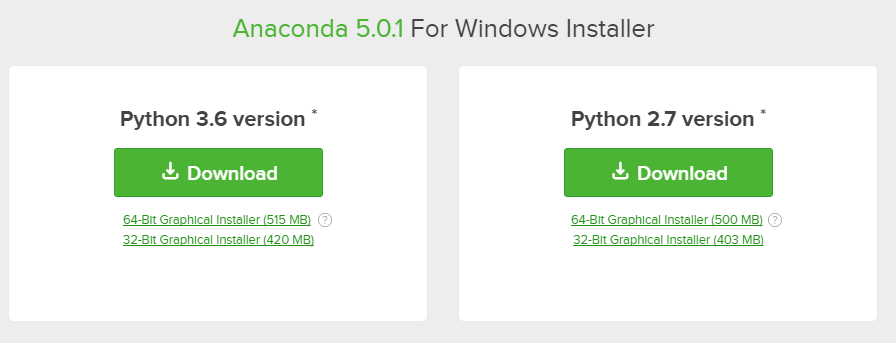
\includegraphics{images/anaconda_python3_or_python2.png}
\caption{Anaconda select Python 3.6}
\end{figure}

You may be prompted to enter your email. You can still download Anaconda
if you click \passthrough{\lstinline![No Thanks]!} and don't enter your
Work Email address.

\begin{figure}
\centering
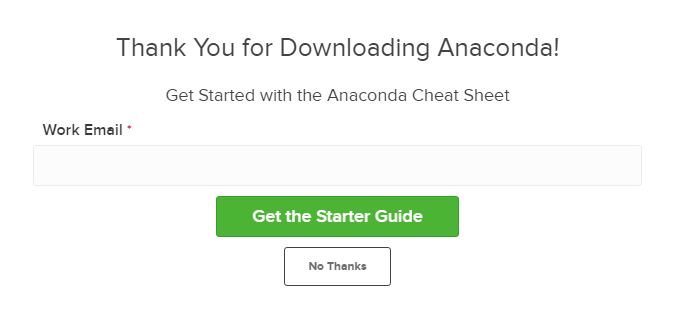
\includegraphics{images/anaconda_enter_email.png}
\caption{anaconda}
\end{figure}

The download is quite large (over 500 MB) so it may take a while to for
Anaconda to download.

\begin{figure}
\centering

\includegraphics{images/anaconda_downloading.png}
\caption{anaconda downloading}
\end{figure}
    




    
        \hypertarget{open-and-run-the-installer}{%
\subsubsection{4. Open and run the
installer}\label{open-and-run-the-installer}}

Once the download completes, open and run the \textbf{\emph{.exe}}
installer

\begin{figure}
\centering
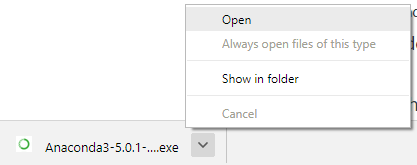
\includegraphics{images/anaconda_run_installer.png}
\caption{anaconda installer}
\end{figure}

At the beginning of the install, you need to click \textbf{Next} to
confirm the installation.

\begin{figure}
\centering
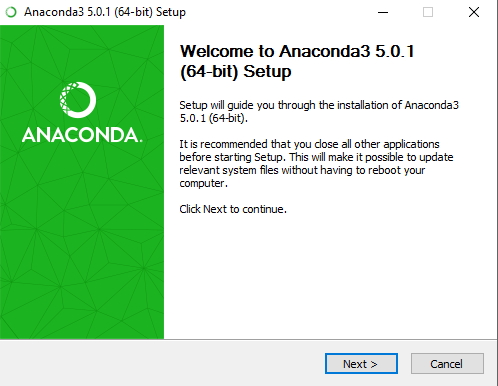
\includegraphics{images/anaconda_installer_click_next.png}
\caption{anaconda installer click next}
\end{figure}

Then agree to the license.

\begin{figure}
\centering
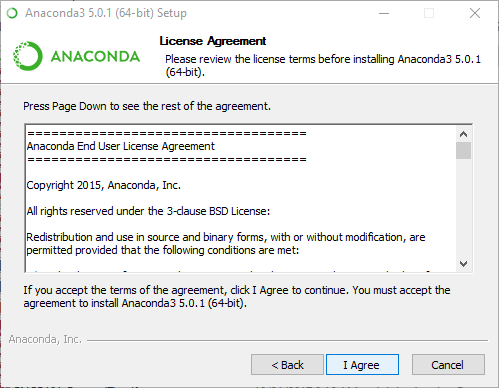
\includegraphics{images/anaconda_agree_to_license.png}
\caption{anaconda license}
\end{figure}

At the Advanced Installation Options screen, I recommend that you
\textbf{do not check} ``Add Anaconda to my PATH environment variable''

\begin{figure}
\centering
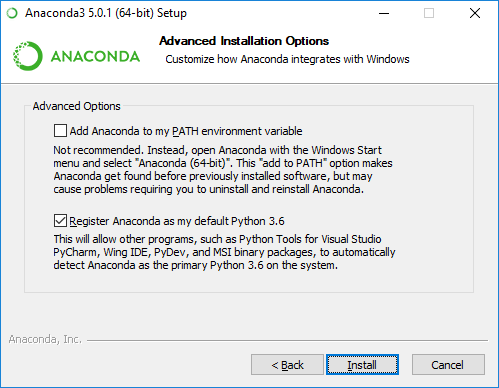
\includegraphics{images/anaconda_path2.png}
\caption{anaconda path variable}
\end{figure}
    




    
        \hypertarget{open-the-anaconda-prompt-from-the-windows-start-menu}{%
\subsubsection{5. Open the Anaconda Prompt from the Windows start
menu}\label{open-the-anaconda-prompt-from-the-windows-start-menu}}

After the installation of Anaconda is complete, you can go to the
Windows start menu and select the Anaconda Prompt.

\begin{figure}
\centering
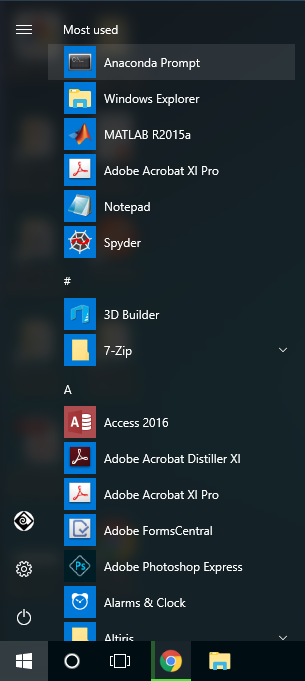
\includegraphics{images/anaconda_from_start_menu.png}
\caption{anaconda in start menu}
\end{figure}

This opens the \textbf{Anaconda Prompt}. \textbf{Anaconda} is the Python
distribution and the \textbf{Anaconda Prompt} is a command line shell (a
program where you type in commands instead of using a mouse). The black
screen and text that makes up the \textbf{Anaconda Prompt} doesn't look
like much, but it is really helpful for problem solvers using Python.

At the Anaconda prompt, type \passthrough{\lstinline!python!} and hit
\passthrough{\lstinline![Enter]!}. The \passthrough{\lstinline!python!}
command starts the Python interpreter, also called the Python REPL (for
Read Evaluate Print Loop).

\begin{lstlisting}
> python
\end{lstlisting}

\begin{figure}
\centering
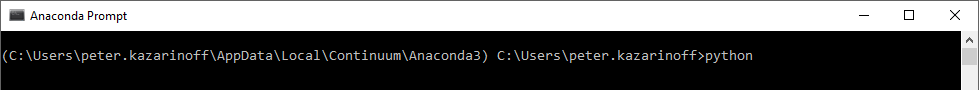
\includegraphics{images/conda_prompt_type_python.png}
\caption{conda prompt type python}
\end{figure}

Note the Python version. You should see something like
\passthrough{\lstinline!Python 3.6.1!}. With the interpreter running,
you will see a set of greater-than symbols \passthrough{\lstinline!>>>!}
before the cursor.

\begin{figure}
\centering
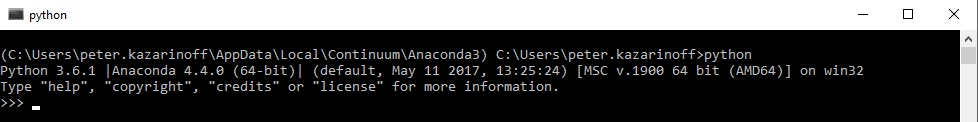
\includegraphics{images/conda_type_python.png}
\caption{anaconda prompt}
\end{figure}

Now you can type Python commands. Try typing
\passthrough{\lstinline!import this!}. You should see the
\textbf{\emph{Zen of Python}} by Tim Peters

\begin{figure}
\centering
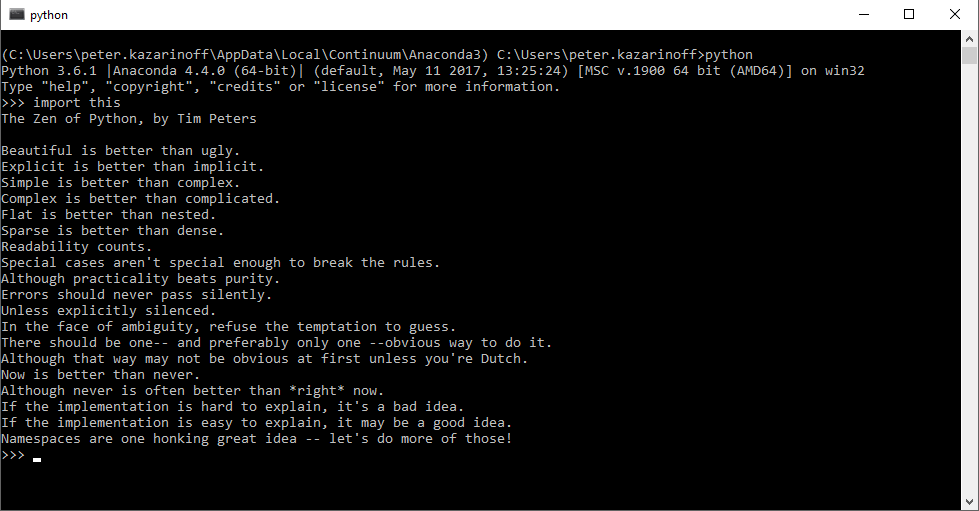
\includegraphics{images/conda_import_this_output.png}
\caption{anaconda\_import\_this}
\end{figure}

To close the Python interpreter, type \passthrough{\lstinline!exit()!}
at the prompt \passthrough{\lstinline!>>>!}. Note the double parenthesis
at the end of the \passthrough{\lstinline!exit()!} command. The
\passthrough{\lstinline!()!} is needed to stop the Python interpreter
and get back out to the \textbf{Anaconda Prompt}.

To close the \textbf{Anaconda Prompt}, you can either close the window
with the mouse, or type \passthrough{\lstinline!exit!}, no parenthesis
necessary.

When you want to use the Python interpreter again, just click the
Windows Start button and select the \textbf{Anaconda Prompt} and type
\passthrough{\lstinline!python!}.
    



    \begin{Verbatim}[commandchars=\\\{\}]
{\color{incolor}In [{\color{incolor} }]:} 
\end{Verbatim}


    
        \hypertarget{installing-anaconda-on-macos}{%
\section{Installing Anaconda on
MacOS}\label{installing-anaconda-on-macos}}
    




    
        This section details the installation of the Anaconda Distribution of
Python on MacOS. Most versions of MacOS come pre-installed with legacy
Python (Version 2.7). You can confirm the legacy version of Python is
installed on MacOS by opening and running a command at the MacOS
\textbf{terminal}. To open the MacOS terminal use
\passthrough{\lstinline![command]+[Space Bar]!} and type
\passthrough{\lstinline!terminal!} in the Spotlight Search bar.

In the MacOS Terminal type (note: the dollar sign
\passthrough{\lstinline!$!} is used to indicate the terminal prompt. The
dollar sign \passthrough{\lstinline!$!} does not need to be typed):

\begin{lstlisting}
$ python
\end{lstlisting}

You will most likely see Python version 2.7 is installed. An issue for
MacOS users is that the installed system version of Python has a set of
permissions that may always allow Python to run and may not allow users
to install external packages. Therefore, I recommend the Anaconda
distribution of Python is installed alongside the system version of
Python that comes pre-installed with MacOS. You will be able to run
Python code using the Anaconda distribution of Python, and you will be
able to install external packages using the Anaconda distribution of
Python.

Follow the steps below to install the Anaconda distribution of Python on
MacOS.

\hypertarget{steps}{%
\subsubsection{Steps:}\label{steps}}

\begin{enumerate}
\def\labelenumi{\arabic{enumi}.}
\item
  Visit
  \href{https://www.anaconda.com/download/}{Anaconda.com/downloads}
\item
  Select MacOS and Download the \textbf{\emph{.pkg}} installer
\item
  Open the \textbf{\emph{.pkg}} installer
\item
  Follow the installation instructions
\item
  Source your \textbf{\emph{.bash-rc}} file
\item
  Open a terminal and type \passthrough{\lstinline!python!} and run some
  code.
\end{enumerate}
    




    
        \hypertarget{visit-the-anaconda-downloads-page}{%
\subsubsection{1. Visit the Anaconda downloads
page}\label{visit-the-anaconda-downloads-page}}

Go to the following link:
\href{https://www.anaconda.com/download/}{Anaconda.com/downloads}

The Anaconda Downloads Page will look something like this:

\begin{figure}
\centering

\includegraphics{images/anaconda_download_page.png}
\caption{anaconda download page}
\end{figure}
    




    
        \hypertarget{select-macos-and-download-the-.pkg-installer}{%
\subsubsection{2. Select MacOS and download the .pkg
installer}\label{select-macos-and-download-the-.pkg-installer}}

In the operating systems box, select \passthrough{\lstinline![MacOS]!}.
Then download the most recent Python 3 distribution (at the time of this
writing the most recent version is Python 3.6) graphical installer by
clicking the Download link. Python 2.7 is legacy Python. For problem
solvers, select the most recent Python 3 version.

\begin{figure}
\centering
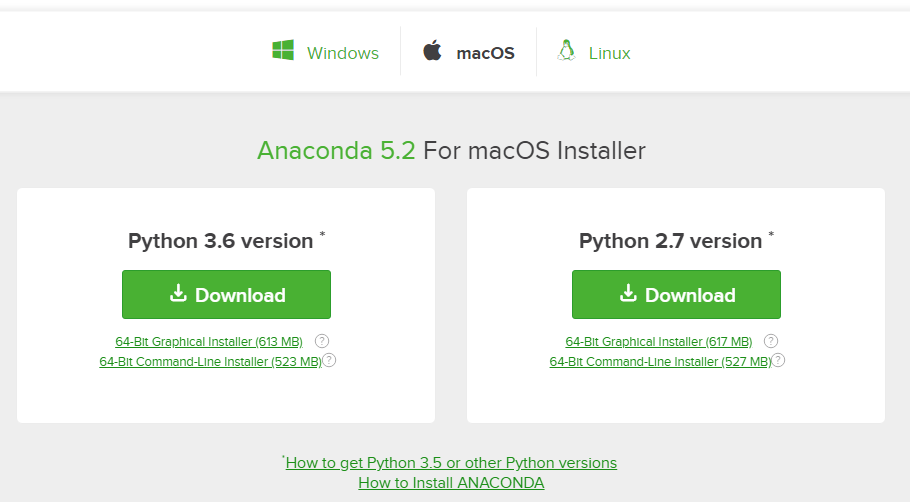
\includegraphics{images/anaconda_download_mac.png}
\caption{Anaconda Select Python 3.6}
\end{figure}

You may be prompted to enter your email. You can still download Anaconda
if you click \passthrough{\lstinline![No Thanks]!} or
\passthrough{\lstinline![x]!} and don't enter your Work Email address.

\begin{figure}
\centering
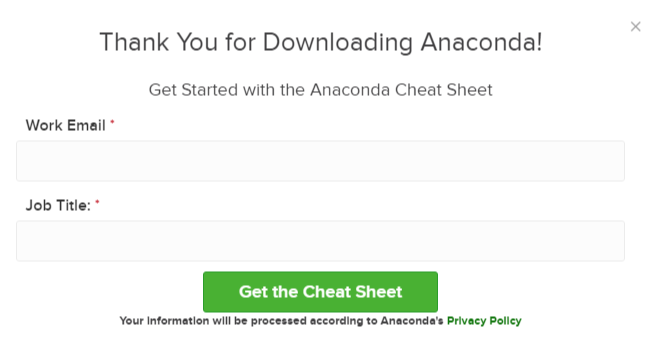
\includegraphics{images/anaconda_download_mac_ask_for_email.png}
\caption{Anaconda ask for email}
\end{figure}
    




    
        \hypertarget{open-the-.pkg-installer}{%
\subsubsection{3. Open the .pkg
installer}\label{open-the-.pkg-installer}}

Navigate to the Downloads folder and double-click the
\textbf{\emph{.pkg}} installer file you just downloaded. It may be
helpful to order the contents of the Downloads folder by date to find
the \textbf{\emph{.pkg}} file.
    




    
        \hypertarget{follow-the-installation-instructions}{%
\subsubsection{4. Follow the installation
instructions}\label{follow-the-installation-instructions}}

Follow the installation instructions. It is advised that you install
\textbf{Anaconda} for the current user and that \textbf{Anaconda}
\textbf{is added to your PATH}.
    




    
        \hypertarget{source-your-.bash-rc-file}{%
\subsubsection{5. Source your .bash-rc
file}\label{source-your-.bash-rc-file}}

Once Anaconda is installed, you need to load the changes to your
\passthrough{\lstinline!PATH!} environment variable in the current
terminal session.

Open the MacOS Terminal and type:

\begin{lstlisting}
$ cd ~
$ source .bashrc
\end{lstlisting}
    




    
        \hypertarget{open-a-terminal-and-type-python-and-run-some-code.}{%
\subsubsection{\texorpdfstring{6. Open a terminal and type
\texttt{python} and run some
code.}{6. Open a terminal and type python and run some code.}}\label{open-a-terminal-and-type-python-and-run-some-code.}}

Open the MacOS Terminal and type:

\begin{lstlisting}
$ python
\end{lstlisting}

You should see something like

\begin{lstlisting}
Python 3.6.3 | Anaconda Inc. |
\end{lstlisting}

At the Python REPL (the Python \passthrough{\lstinline!>>>!} prompt)
try:

\begin{lstlisting}
>>> import this
\end{lstlisting}

If you see the Zen of Python, the installation was successful. Exit out
of the Python REPL using the command \passthrough{\lstinline!exit()!}.
Make sure to include the double parenthesis \passthrough{\lstinline!()!}
after the \passthrough{\lstinline!exit!} command.

\begin{lstlisting}
>>> exit()
\end{lstlisting}
    



    \begin{Verbatim}[commandchars=\\\{\}]
{\color{incolor}In [{\color{incolor} }]:} 
\end{Verbatim}


    
        \hypertarget{installing-anaconda-on-linux}{%
\section{Installing Anaconda on
Linux}\label{installing-anaconda-on-linux}}
    




    
        This section details the installation of the Anaconda distribution of
Python on Linux, specifically Ubuntu 18.04, but the instructions should
work for other Debian-based Linux distributions as well.

Ubuntu 18.04 comes pre-installed with Python (Version 3.6) and legacy
Python (Version 2.7). You can confirm the legacy version of Python is
installed by opening up a terminal.

In the terminal type:

\begin{lstlisting}
$ python
\end{lstlisting}

You will most likely see Python Version 2.7 is installed. If you enter:

\begin{lstlisting}
$ python3
\end{lstlisting}

You will most likely see Python Version 3.6 is also installed. You can
use the 3.6 Version of Python, but each time a new package needs to be
downloaded, the \passthrough{\lstinline!$ pip3 install!} command must be
used.

Install the Anaconda distribution of Python to follow the examples in
the book without the need to install additional third-party packages.
    




    
        \hypertarget{steps}{%
\subsubsection{Steps:}\label{steps}}

\begin{enumerate}
\def\labelenumi{\arabic{enumi}.}
\item
  Visit
  \href{https://www.anaconda.com/download/}{Anaconda.com/downloads}
\item
  Select Linux
\item
  Copy the bash (.sh file) installer link
\item
  Use \passthrough{\lstinline!wget!} to download the bash installer
\item
  Run the bash script to install \textbf{Anaconda3}
\item
  \passthrough{\lstinline!source!} the
  \passthrough{\lstinline!.bash-rc!} file to add Anaconda to your
  \passthrough{\lstinline!PATH!}
\item
  Start the Python REPL
\end{enumerate}
    




    
        \hypertarget{visit-the-anaconda-downloads-page}{%
\subsection{1. Visit the Anaconda downloads
page}\label{visit-the-anaconda-downloads-page}}

Go to the following link:
\href{https://www.anaconda.com/download/}{Anaconda.com/downloads}

The Anaconda Downloads Page will look something like this:

\begin{figure}
\centering

\includegraphics{images/anaconda_download_page.png}
\caption{Anaconda Downloads Page}
\end{figure}
    




    
        \hypertarget{select-linux}{%
\subsection{2. Select Linux}\label{select-linux}}

On the downloads page, select the Linux operating system

\begin{figure}
\centering

\includegraphics{images/Anaconda_download_linux.png}
\caption{anaconda\_install\_linux}
\end{figure}
    




    
        \hypertarget{copy-the-bash-.sh-file-installer-link}{%
\subsection{3. Copy the bash (.sh file) installer
link}\label{copy-the-bash-.sh-file-installer-link}}

In the \textbf{Python 3.6 Version* } box, right-click on the
{[}64-Bit(x86) Installer{]} link. Select {[}copy link address{]}.

\begin{figure}
\centering
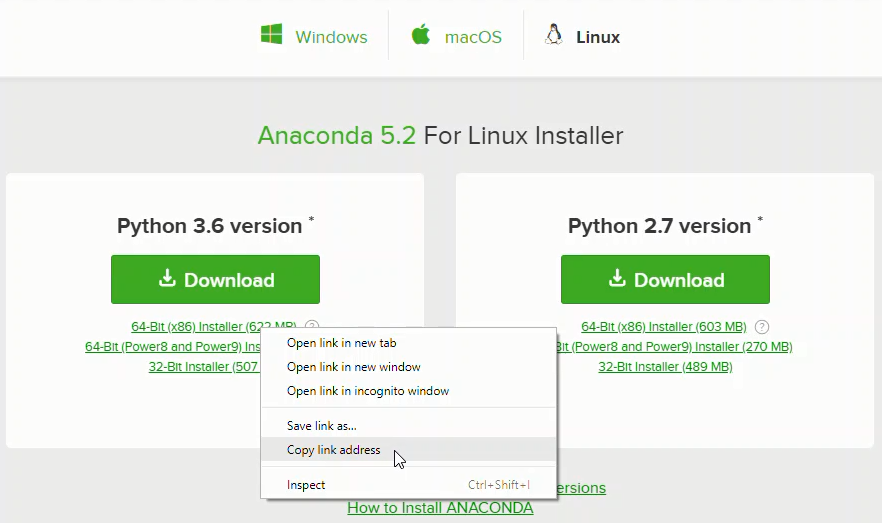
\includegraphics{images/anaconda_install_linux_copy_link_address.png}
\caption{Anaconda installation on Linux copy link address}
\end{figure}
    




    
        \hypertarget{use-wget-to-download-the-bash-installer}{%
\subsection{\texorpdfstring{4. Use \texttt{wget} to download the bash
installer}{4. Use wget to download the bash installer}}\label{use-wget-to-download-the-bash-installer}}

Now that the bash installer (.sh file) link is stored on the clipboard,
use \passthrough{\lstinline!wget!} to download the installer script. In
a terminal, \passthrough{\lstinline!cd!} into the home directory and
make a new directory called \passthrough{\lstinline!tmp!}.
\passthrough{\lstinline!cd!} into \passthrough{\lstinline!tmp!} and use
\passthrough{\lstinline!wget!} to download the installer. Although the
installer is a bash script, it is still quite large and the download
will not be immediate.

\begin{lstlisting}
$ cd ~
$ mkdir tmp
$ cd tmp
$ wget https://repo.anaconda.com/archive/Anaconda3-5.2.0-Linux-x86_64.sh 
\end{lstlisting}
    




    
        \hypertarget{run-the-bash-script-to-install-anaconda3}{%
\subsection{\texorpdfstring{5. Run the bash script to install
\textbf{Anaconda3}}{5. Run the bash script to install Anaconda3}}\label{run-the-bash-script-to-install-anaconda3}}

With the bash installer script downloaded, run the \textbf{\emph{.sh}}
script to install \textbf{Anaconda3}. Ensure you are in the directory
where the installer script downloaded:

\begin{lstlisting}
$ ls
Anaconda3-5.2.0-Linux-x86_64.sh
\end{lstlisting}

Run the installer script with bash.

\begin{lstlisting}
$ bash Anaconda3-5.2.0-Linux-x86_64.sh
\end{lstlisting}

Accept the Licence Agreement and allow Anaconda to be added to your
\passthrough{\lstinline!PATH!}. By adding Anaconda to your
\passthrough{\lstinline!PATH!}, the Anaconda distribution of Python will
be called when you type \passthrough{\lstinline!$ python!} in a
terminal.
    




    
        \hypertarget{source-the-.bash-rc-file-to-add-anaconda-to-your-path}{%
\subsubsection{\texorpdfstring{6. \texttt{source} the \texttt{.bash-rc}
file to add Anaconda to your
\texttt{PATH}}{6. source the .bash-rc file to add Anaconda to your PATH}}\label{source-the-.bash-rc-file-to-add-anaconda-to-your-path}}

Now that \textbf{Anaconda3} is installed and \textbf{Anaconda3} is added
to our \passthrough{\lstinline!PATH!}, \passthrough{\lstinline!source!}
the \passthrough{\lstinline!.bashrc!} file to load the new
\passthrough{\lstinline!PATH!} environment variable into the current
terminal session. Note the \passthrough{\lstinline!.bashrc!} file is in
the home directory. You can see it with
\passthrough{\lstinline!$ ls -a!}.

\begin{lstlisting}
$ cd ~
$ source .bashrc
\end{lstlisting}
    




    
        \hypertarget{start-the-python-repl}{%
\subsubsection{7. Start the Python REPL}\label{start-the-python-repl}}

To verify the installation is complete, open Python from the command
line:

\begin{lstlisting}
$ python

Python 3.6.5 |Anaconda, Inc.| (default, Mar 29 2018, 18:21:58)
[GCC 7.2.0] on linux
Type "help", "copyright", "credits" or "license" for more information.
>>>
\end{lstlisting}

If you see Python 3.6 from Anaconda listed, your installation is
complete. To exit the Python REPL, type:

\begin{lstlisting}
>>> exit()
\end{lstlisting}
    



    \begin{Verbatim}[commandchars=\\\{\}]
{\color{incolor}In [{\color{incolor} }]:} 
\end{Verbatim}


    
        \hypertarget{installing-python-from-python.org}{%
\section{Installing Python from
Python.org}\label{installing-python-from-python.org}}
    




    
        Below is the recommended way to install a new version of Python from
Python.org on each of the three major operating systems: Windows, MacOS
and Linux.

This book is based on Python version 3.6. Some of the examples in the
book may not work properly on legacy Python (version 2.7). I recommend
installing the Anaconda Distribution of Python on Windows and MacOSX.
The installation of Anaconda on these operating systems was detailed in
previous sections.
    




    
        \hypertarget{installing-python-on-windows}{%
\subsection{Installing Python on
Windows}\label{installing-python-on-windows}}

Go to \url{https://www.python.org/downloads/} and download the latest
release. Make sure to select the box
\passthrough{\lstinline![add Python to my path]!} during the
installation.

\begin{figure}
\centering
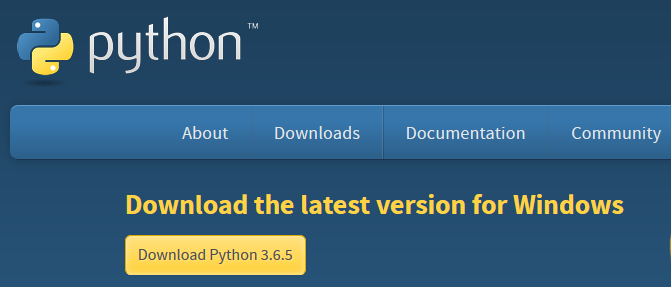
\includegraphics{images/python_dot_org_windows_download.PNG}
\caption{Python.org download for Windows}
\end{figure}
    




    
        \hypertarget{installing-python-on-macos}{%
\subsection{Installing Python on
MacOS}\label{installing-python-on-macos}}

Go to \url{https://www.python.org/downloads/mac-osx/} and download the
latest release.

\begin{figure}
\centering

\includegraphics{images/python_dot_org_macos_download.PNG}
\caption{Python.org download for MacOS}
\end{figure}
    




    
        \hypertarget{installing-python-on-linux}{%
\subsection{Installing Python on
Linux}\label{installing-python-on-linux}}

Open a terminal and enter \passthrough{\lstinline!$ python!} to see if a
version of Python is already installed on the system.

\begin{lstlisting}
$ python
Python 2.7.12 (default, Dec  4 2017, 14:50:18)
[GCC 5.4.0 20160609] on linux2
Type "help", "copyright", "credits" or "license" for more information.
>>> exit()
\end{lstlisting}

In the code block above, the version of Python is
\passthrough{\lstinline!Python 2.7.12!}. If the Python version is 2.7 or
below, try the command \passthrough{\lstinline!$ python3!}.

\begin{lstlisting}
$ python3
Python 3.6.7 (default, Oct 22 2018, 11:32:17) 
[GCC 8.2.0] on linux
Type "help", "copyright", "credits" or "license" for more information.
>>> exit()
\end{lstlisting}

If no version of Python is shown, you can download a release of Python
3.6 from the deadsnakes package repository.

\begin{lstlisting}
$ sudo add-apt-repository ppa:deadsnakes/ppa
[Enter]
$ sudo apt-get update
$ sudo apt-get install python3.6
\end{lstlisting}

After installation, you may need to append your PATH environment
variable to ensure the newly installed Python 3.6 version is the version
of Python called when using the terminal. The commands below will add
\passthrough{\lstinline!/usr/bin!} to your
\passthrough{\lstinline!PATH!}, and add an alias in
\textbf{\emph{.bashrc}} so that the command
\passthrough{\lstinline!$ python3.6!} produces the Python 3.6 REPL. Take
care to ensure the double chevron \passthrough{\lstinline!>>!} is used,
as a single chevron \passthrough{\lstinline!>!} will overwrite the
\textbf{\emph{.bashrc}} file.

\begin{lstlisting}
$ cd ~
$ echo  "PATH=/usr/bin:$PATH" >> ~/.bashrc 
$ echo "alias python3.6='/usr/bin/python3.6'" >> ~/.bashrc
$ source .bashrc
$ python3.6
Python 3.6.6 (default, Jun 28 2018, 04:42:43)
[GCC 5.4.0 20160609] on linux
Type "help", "copyright", "credits" or "license" for more information.
>>> exit()
\end{lstlisting}
    



    \begin{Verbatim}[commandchars=\\\{\}]
{\color{incolor}In [{\color{incolor} }]:} 
\end{Verbatim}


    
        \newpage
        \hypertarget{summary}{%
\section{Summary}\label{summary}}

    




    
        In this chapter, you learned about the Anaconda distribution of Python
and how the Anaconda distribution of Python compares the version of
Python at Python.org. The Anaconda distribution of Python comes with
about 600 packages pre-installed as well as Jupyter notebooks and the
Anaconda Prompt. Jupyter notebooks and some of the pre-installed
packages that come with Anaconda will be used later chapters. This text
recommends that problem solvers install the Anaconda distribution of
Python.

This chapter showed how to install the Anaconda distribution of Python
on Windows, MacOS, and Linux.

At the end of the chapter, a description of how to download and install
Python from Python.org was shown.
    




    
        \hypertarget{key-terms-and-concepts}{%
\subsection{Key Terms and Concepts}\label{key-terms-and-concepts}}
    




    
        \begin{key_terms}
        Anaconda

Anaconda Prompt

download

install

Python

Legacy Python

Python Interpreter

Python REPL

package

operating system

Windows

MacOS

Linux

terminal

PATH
        \end{key_terms}

    



    \begin{Verbatim}[commandchars=\\\{\}]
{\color{incolor}In [{\color{incolor} }]:} 
\end{Verbatim}


    
        \hypertarget{review-questions}{%
\section{Review Questions}\label{review-questions}}
    




    
        \begin{problems}
        Q01.01 What is Python? How is the Python language different than the
Python Interpreter?

Q01.02 What is the difference between the version of Python at
python.org and the version of Python at Anaconda.com?

Q01.03 What are the advantages and disadvantages of using the Anaconda
distribution of Python compared to using the version of Python at
python.org?

Q01.04 There are many different applications to edit Python code. Some
examples include: JupyterLab, Sublime Text, Visual Studio Code, and
PyCharm. Pick two Python code editors and explain a feature of each code
editor.

Q01.05 What are some advantages of Python compared to other computer
programming languages?

Q01.06 What is PyPI? How many packages are currently available for
download on PyPI?

Q01.07 Find three modules that are part of the Python Standard Library.
Write a short description of what each of the modules you choose is used
for.

Q01.08 Which computer operating systems can Python be installed on?

Q01.09 How much does Python cost to download and install?

Q01.10 What are three subject areas that have seen a growth in the use
of Python.

Q01.11 Besides PyPI where else can problem solvers go to find Python
packages, scripts, and utilities?

Q01.12 Name three packages that come pre-installed with the Anaconda
distribution of Python

Q01.13 How much does the Anaconda distribution of Python cost to
download and install?

Q01.14 Which operating systems can the Anaconda distribution of Python
be installed on?

Q01.15 What type of program is the Anaconda Prompt?

Q01.16 What is another name for the Python interpreter?

Q01.17 How can you bring up the Python interpreter (the Python REPL)
using the Anaconda Prompt?

Q01.18 What prompt is shown in the Python interpreter (the Python REPL)?

Q01.19 What command do you type to close the Python interpreter (the
Python REPL)?

Q01.20 What are the first three lines in \emph{The Zen of Python} by Tim
Peters?

Q01.21 How do you open the Anaconda Prompt?
        \end{problems}

    




    
        \hypertarget{installing-python-on-macos}{%
\subsubsection{Installing Python on
MacOS}\label{installing-python-on-macos}}
    




    
        \begin{problems}
        Q01.30 What web address do you go to download the Anaconda distribution
of Python for MacOS?

Q01.31 What file extension does the installer for MacOS of the Anaconda
distribution of Python use?

Q01.32 When you install the Anaconda distribution of Python on MacOS,
what is advised to do for the installation options?

Q01.33 Why do you need to \passthrough{\lstinline!source!} the
\textbf{\emph{.bashrc}} file after you install the Anaconda distribution
of Python for MacOS?

Q01.34 How can you bring up the Python interpreter (the Python REPL)
using the MacOS terminal?

Q01.35 Which version of Python is it advisable to download and install
on MacOS?

Q01.36 Python can be installed on MacOS using a terminal program called
\textbf{Homebrew}. What command is issued to the MacOS terminal to
install Python using \textbf{Homebrew}?

Q01.37 What version of Python comes pre-installed on MacOS?
        \end{problems}

    




    
        \hypertarget{installing-python-on-linux}{%
\subsubsection{Installing Python on
Linux}\label{installing-python-on-linux}}
    




    
        \begin{problems}
        Q01.40 What version(s) of Python comes pre-installed on most Linux
distributions?

Q01.41 In Linux, what happens when you type
\passthrough{\lstinline!python!} at the terminal compared to when you
type \passthrough{\lstinline!python3!} at the terminal?

Q01.42 If you use the system version of Python 3 installed on Linux,
what command must you enter to install Python packages to the Python 3
version that comes pre-installed?

Q01.43 What kind of file type (what is the file extension) is downloaded
from Anaconda.com to install the Anaconda distribution of Python on
Linux?

Q01.44 Why do you need to \passthrough{\lstinline!source!} the
\textbf{\emph{.bashrc}} file after you install the Anaconda distribution
of Python for Linux?

Q01.45 How can you bring up the Python interpreter (the Python REPL)
using a Linux terminal?

Q01.46 Which version of Python is it advisable to download and install
on Linux?

Q01.47 What is a disadvantage of using the version of Python that comes
pre-installed on Linux, compared to using the Anaconda distribution of
Python on Linux?

Q01.48 Before you install the Anaconda distribution of Python on Linux,
what version of Python are you most likely to see when you enter the
command \passthrough{\lstinline!$ python!} in a Linux terminal?

Q01.49 Before you install the Anaconda distribution of Python on Linux,
what version of Python are you most likely to see when you enter the
command \passthrough{\lstinline!$ python3!} in a Linux terminal?
        \end{problems}

    




    
        \hypertarget{installing-python-from-python.org}{%
\subsubsection{Installing Python from
Python.org}\label{installing-python-from-python.org}}
    




    
        \begin{problems}
        Q01.50 What web address do you go to download Python from Python.org?

Q01.51 What option is advised to select when downloading and installing
Python from Python.org on Windows?

Q01.52 If Python 3 is not available on Linux, what package repository
can Python 3.6 be downloaded from?

Q01.53 Go to Python.org. What is the current version of Python available
for download?
        \end{problems}

    




    
        \hypertarget{errors-explanations-and-solutions}{%
\subsubsection{Errors, Explanations, and
Solutions}\label{errors-explanations-and-solutions}}
    




    
        \begin{problems}
        For each of the problems below, run the line of code. Copy the output,
then suggest and run a line of code that fixes the error.

Q01.91 Open the Python Interpreter (the Python REPL). Try to close the
Python Interpreter with the command:

\begin{lstlisting}
>>> exit
\end{lstlisting}

Q02.92 Open the Python Interpreter (the Python REPL). Try to view
\emph{The Zen of Python} by Tim Peters with the command:

\begin{lstlisting}
>>> Zen of Python
\end{lstlisting}

Q01.93 Open the Anaconda Prompt. Try to open the Python Interpreter (the
Python REPL) with the command:

\begin{lstlisting}
> python3
\end{lstlisting}

Q01.94 Open the Anaconda Prompt. Try to open the Python Interpreter (the
Python REPL) with the command:

\begin{lstlisting}
> Python
\end{lstlisting}

Q02.95 Open the Python Interpreter (the Python REPL). Try to view
\emph{The Zen of Python} by Tim Peters with the command:

\begin{lstlisting}
>>> import this()
\end{lstlisting}
        \end{problems}

    



    \begin{Verbatim}[commandchars=\\\{\}]
{\color{incolor}In [{\color{incolor} }]:} 
\end{Verbatim}


    
        \hypertarget{the-python-repl}{%
\chapter{The Python REPL}\label{the-python-repl}}
    




    
        \hypertarget{introduction}{%
\section{Introduction}\label{introduction}}
    




    
        By the end of this chapter, you will be able to:

\begin{itemize}
\item
  Open and close the Python REPL
\item
  Compute mathematical calculations using the Python REPL
\item
  Use the output from Python REPL as input in another problem
\item
  Import the math and statistics modules from the Python Standard
  Library and use their functions
\item
  Assign values to variables
\item
  Use variables in calculations
\item
  Create strings
\item
  Combine, compare, and pull characters out of strings
\end{itemize}
        \newpage



    



    \begin{Verbatim}[commandchars=\\\{\}]
{\color{incolor}In [{\color{incolor} }]:} 
\end{Verbatim}


    
        \hypertarget{python-as-a-calculator}{%
\section{Python as a Calculator}\label{python-as-a-calculator}}
    




    
        Python can be used as a calculator to compute arithmetic operations like
addition, subtraction, multiplication and division. Python can also be
used for trigonometric calculations and statistical calculations.
    




    
        \hypertarget{arithmetic}{%
\subsection{Arithmetic}\label{arithmetic}}

Python can be used as a calculator to make simple arithmetic
calculations.

Simple arithmetic calculations can be completed at the Python Prompt,
also called the \emph{Python REPL}. REPL stands for Read Evaluate Print
Loop. The Python REPL shows three arrow symbols
\passthrough{\lstinline!>>>!} followed by a blinking cursor. Programmers
type commands at the \passthrough{\lstinline!>>>!} prompt then hit
\passthrough{\lstinline![ENTER]!} to see the results.

Commands typed into the Python REPL are \emph{read} by the interpreter,
results of running the commands are \emph{evaluated}, then
\emph{printed} to the command window. After the output is printed, the
\passthrough{\lstinline!>>>!} prompt appears on a new line. This process
repeats over and over again in a continuous \emph{loop}.

Try the following commands at the Python REPL:

Suppose the mass of a battery is 5 kg and the mass of the battery cables
is 3 kg. What is the mass of the battery cable assembly?

\begin{lstlisting}[language=Python]
>>> 5 + 3
8
\end{lstlisting}

Suppose one of the cables above is removed and it has a mass of 1.5 kg.
What is the mass of the leftover assembly?

\begin{lstlisting}[language=Python]
>>> 8 - 1.5
6.5
\end{lstlisting}

If the battery has a mass of 5000 g and a volume of 2500 \(cm^3\) What
is the density of the battery? The formula for density is below, where
\(D\) is density, \(m\) is mass and \(v\) is volume.

\[ D = \frac{m}{v} \]

In the problem above \(m = 5000\) and \(v=2500\)

Let's solve this with Python.

\begin{lstlisting}[language=Python]
>>> 5000 / 2500
2.0
\end{lstlisting}

What is the total mass if we have 2 batteries, and each battery weighs 5
kg?

\begin{lstlisting}[language=Python]
>>> 5 * 2
2.0
\end{lstlisting}

The length, width, and height of each battery is 3 cm. What is the area
of the base of the battery? To complete this problem, use the double
asterisk symbol \passthrough{\lstinline!**!} to raise a number to a
power.

\begin{lstlisting}[language=Python]
>>> 3 ** 2
9
\end{lstlisting}

What is the volume of the battery if each the length, width, and height
of the battery are all 3 cm?

\begin{lstlisting}[language=Python]
>>> 3 ** 3
27
\end{lstlisting}

Find the mass of the two batteries and two cables.

We can use Python to find the mass of the batteries and then use the
answer, which Python saves as an underscore \_ to use in our next
operation. (The underscore \passthrough{\lstinline!\_!} in Python is
comparable to the \passthrough{\lstinline!ans!} variable in MATLAB)

\begin{lstlisting}[language=Python]
>>> 2 * 5 
10
>>> _ + 1.5 + 1
12.5
\end{lstlisting}
    




    
        \hypertarget{section-summary}{%
\subsubsection{Section Summary}\label{section-summary}}

A summary of the arithmetic operations in Python is below:

\begin{longtable}[]{@{}lllll@{}}
\toprule
operator & name & description & example & result\tabularnewline
\midrule
\endhead
\passthrough{\lstinline!+!} & addition & adds two numbers &
\passthrough{\lstinline!2 + 3!} &
\passthrough{\lstinline!5!}\tabularnewline
\passthrough{\lstinline!-!} & subtraction & subtracts two numbers &
\passthrough{\lstinline!8 - 6!} &
\passthrough{\lstinline!2!}\tabularnewline
\passthrough{\lstinline!-!} & negation & negative number &
\passthrough{\lstinline!-4!} &
\passthrough{\lstinline!-4!}\tabularnewline
\passthrough{\lstinline!*!} & multiplication & multiplies two numbers &
\passthrough{\lstinline!5 * 2!} &
\passthrough{\lstinline!10!}\tabularnewline
\passthrough{\lstinline!/!} & division & divides two numbers &
\passthrough{\lstinline!6 / 3!} &
\passthrough{\lstinline!2!}\tabularnewline
\passthrough{\lstinline!**!} & exponents & raises a number to a power &
\passthrough{\lstinline!10**2!} &
\passthrough{\lstinline!100!}\tabularnewline
\passthrough{\lstinline!\_!} & underscore & returns last saved value &
\passthrough{\lstinline!\_ + 7!} &
\passthrough{\lstinline!107!}\tabularnewline
\bottomrule
\end{longtable}
    




    
        \hypertarget{trigonometry-sine-cosine-and-tangent}{%
\subsection{Trigonometry: sine, cosine, and
tangent}\label{trigonometry-sine-cosine-and-tangent}}
    




    
        Trigonometry functions such as sine, cosine, and tangent can also be
calculated using the Python REPL.

To use Python's trig functions, we need to introduce a new concept:
\emph{importing modules}.

In Python, there are many operations built into the language when the
REPL starts. These include \passthrough{\lstinline!+!} ,
\passthrough{\lstinline!-!}, \passthrough{\lstinline!*!},
\passthrough{\lstinline!/!} like we saw in the previous section.
However, not all functions will work right away when Python starts. Say
we want to find the sine of an angle. Try the following:

\begin{lstlisting}[language=Python]
>>> sin(60)
Traceback (most recent call last):
  File "<stdin>", line 1, in <module>
NameError: name 'sin' is not defined
\end{lstlisting}

This error results because we have not told Python to include the
\passthrough{\lstinline!sin!} function. The
\passthrough{\lstinline!sin!} function is part of the \emph{Python
Standard Library}. The Python Standard Library comes with every Python
installation and includes many functions, but not all of these functions
are available to us when we start a new Python REPL session. To use
Python's \passthrough{\lstinline!sin!} function, first import the
\passthrough{\lstinline!sin!} function from the
\passthrough{\lstinline!math!} \emph{module} which is part of the Python
Standard Library.

Importing modules and functions is easy. Use the following syntax:

\begin{lstlisting}
from module import function
\end{lstlisting}

To import the \passthrough{\lstinline!sin()!} function from the
\passthrough{\lstinline!math!} module try:

\begin{lstlisting}[language=Python]
>>> from math import sin
>>> sin(60)
-0.3048106211022167
\end{lstlisting}

Success! Multiple modules can be imported at the same time. Say we want
to use a bunch of different trig functions to solve the following
problem.

An angle has a value of \(\pi\)/6 radians. What is the sine, cos, and
tangent of the angle?

To solve this problem we need to import the
\passthrough{\lstinline!sin()!}, \passthrough{\lstinline!cos()!}, and
\passthrough{\lstinline!tan()!} functions. It is also useful to have the
value of \(\pi\), rather than having to write
\passthrough{\lstinline!3.14....!} We can import all of these functions
at the same time using the syntax:

\begin{lstlisting}
from module import function1, function2, function3
\end{lstlisting}

Note the commas in between the function names.

Try:

\begin{lstlisting}[language=Python]
>>> from math import sin, cos, tan, pi
>>> pi
3.141592653589793
>>> sin(pi/6)
0.49999999999999994
>>> >>> cos(pi/6)
0.8660254037844387
>>> tan(pi/6)
0.5773502691896257
\end{lstlisting}
    




    
        \hypertarget{section-summary}{%
\subsubsection{Section Summary}\label{section-summary}}

The following trig functions are part of Python's \textbf{math} module:

\begin{longtable}[]{@{}lllll@{}}
\toprule
trig function & name & description & example & result\tabularnewline
\midrule
\endhead
\passthrough{\lstinline!math.pi!} & pi & mathematical constant \(\pi\) &
\passthrough{\lstinline!math.pi!} &
\passthrough{\lstinline!3.14!}\tabularnewline
\passthrough{\lstinline!math.sin()!} & sine & sine of an angle in
radians & \passthrough{\lstinline!math.sin(4)!} &
\passthrough{\lstinline!9.025!}\tabularnewline
\passthrough{\lstinline!math.cos()!} & cosine & cosine of an angle in
radians & \passthrough{\lstinline!cos(3.1)!} &
\passthrough{\lstinline!400!}\tabularnewline
\passthrough{\lstinline!math.tan()!} & tangent & tangent of an angle in
radians & \passthrough{\lstinline!tan(100)!} &
\passthrough{\lstinline!2.0!}\tabularnewline
\passthrough{\lstinline!math.asin()!} & arc sine & inverse sine, ouput
in radians & \passthrough{\lstinline!math.sin(4)!} &
\passthrough{\lstinline!9.025!}\tabularnewline
\passthrough{\lstinline!math.acos()!} & arc cosine & inverse cosine,
ouput in radians & \passthrough{\lstinline!log(3.1)!} &
\passthrough{\lstinline!400!}\tabularnewline
\passthrough{\lstinline!math.atan()!} & arc tangent & inverse tangent,
ouput in radians & \passthrough{\lstinline!atan(100)!} &
\passthrough{\lstinline!2.0!}\tabularnewline
\passthrough{\lstinline!math.radians()!} & radians conversion & degrees
to radians & \passthrough{\lstinline!math.radians(90)!} &
\passthrough{\lstinline!1.57!}\tabularnewline
\passthrough{\lstinline!math.degress()!} & degree conversion & radians
to degrees & \passthrough{\lstinline!math.degrees(2)!} &
\passthrough{\lstinline!114.59!}\tabularnewline
\bottomrule
\end{longtable}
    




    
        \hypertarget{exponents-and-logarithms}{%
\subsection{Exponents and Logarithms}\label{exponents-and-logarithms}}

Calculating exponents and logarithms with Python is easy. Note the
exponent and logarithm functions are imported from the \textbf{math}
module just like the trig functions were imported from the \textbf{math}
module above.

The following exponents and logarithms functions can be imported from
Python's math module:

\begin{itemize}
\tightlist
\item
  \passthrough{\lstinline!log!}
\item
  \passthrough{\lstinline!log10!}
\item
  \passthrough{\lstinline!exp!}
\item
  \passthrough{\lstinline!e!}
\item
  \passthrough{\lstinline!pow(x,y)!}
\item
  \passthrough{\lstinline!sqrt!}
\end{itemize}

Let's try a couple of examples:

\begin{lstlisting}[language=Python]
>>> from math import log, log10, exp, e, pow, sqrt
>>> log(3.0*e**3.4)         # note: natural log
4.4986122886681095
\end{lstlisting}

A right triangle has side lengths 3 and 4. What is the length of the
hypotenuse?

\begin{lstlisting}[language=Python]
>>> sqrt(3**2 + 4**2)
5.0 
\end{lstlisting}

The power function \passthrough{\lstinline!pow()!} works like the
\passthrough{\lstinline!**!} operator to raise a number to a power.

\begin{lstlisting}[language=Python]
>>> 5**2
25
\end{lstlisting}

\begin{lstlisting}[language=Python]
>>> pow(5,2)
25.0
\end{lstlisting}

\hypertarget{section-summary}{%
\subsubsection{Section Summary}\label{section-summary}}

The following exponent and logarithm functions are part of Python's
\textbf{math} module:

\begin{longtable}[]{@{}lllll@{}}
\toprule
math module function & name & description & example &
result\tabularnewline
\midrule
\endhead
\passthrough{\lstinline!math.e!} & euler's number & mathematical
constant \(e\) & \passthrough{\lstinline!math.e!} &
\passthrough{\lstinline!2.718!}\tabularnewline
& & & &\tabularnewline
\passthrough{\lstinline!math.exp()!} & exponent & \(e\) raised to a
power & \passthrough{\lstinline!math.exp(2.2)!} &
\passthrough{\lstinline!9.025!}\tabularnewline
\passthrough{\lstinline!math.log()!} & natural logerithm & log base e &
\passthrough{\lstinline!math.log(3.1)!} &
\passthrough{\lstinline!400!}\tabularnewline
\passthrough{\lstinline!math.log10()!} & base 10 logerithm & log base 10
& \passthrough{\lstinline!math.log10(100)!} &
\passthrough{\lstinline!2.0!}\tabularnewline
\passthrough{\lstinline!math.pow()!} & exponents & raises a number to a
power & \passthrough{\lstinline!math.pow(2,3)!} &
\passthrough{\lstinline!8.0!}\tabularnewline
\passthrough{\lstinline!math.sqrt()!} & square root & square root of a
number & \passthrough{\lstinline!math.sqrt(16)!} &
\passthrough{\lstinline!4.0!}\tabularnewline
\bottomrule
\end{longtable}
    




    
        \hypertarget{statistics}{%
\subsection{Statistics}\label{statistics}}

To round out this section, we will look at a couple of statistics
functions. These functions are part of the Python Standard Library, but
not part of the \textbf{math} module. To access Python's statistics
functions, we need to import them from the \textbf{statistics} module
using the statement
\passthrough{\lstinline!from statistics import mean, median, mode, stdev!}.
Then the functions \passthrough{\lstinline!mean!},
\passthrough{\lstinline!median!}, \passthrough{\lstinline!mode!} and
\passthrough{\lstinline!stdev!}(standard deviation) can be used.

\begin{lstlisting}[language=Python]
>>> from statistics import mean, median, mode, stdev
    
>>> test_scores = [60, 83, 83, 91, 100]
    
>>> mean(test_scores)
83.4

>>> median(test_scores)
83

>>> mode(test_scores)
83
    
>>> stdev(test_scores)
14.842506526863986 
\end{lstlisting}

Alternatively, we can import the entire \textbf{statistics} module using
the statement \passthrough{\lstinline!import statistics!}. Then to use
the functions, we need to use the names
\passthrough{\lstinline!statistics.mean!},
\passthrough{\lstinline!statistics.median!},
\passthrough{\lstinline!statistics.mode!}, and
\passthrough{\lstinline!statistics.stdev!}. See below:

\begin{lstlisting}[language=Python]
>>> import statistics
    
>>> test_scores = [60, 83, 83, 91, 100 ]
    
>>> statistics.mean(test_scores)
83.4

>>> statistics.median(test_scores)
83

>>> statistics.mode(test_scores)
83
    
>>> statistics.stdev(test_scores)
14.842506526863986 
\end{lstlisting}
    




    
        \hypertarget{section-summary}{%
\subsubsection{Section Summary}\label{section-summary}}

The following functions are part of Python's \textbf{statistics} module:

\begin{longtable}[]{@{}lllll@{}}
\toprule
statistics module function & name & description & example &
result\tabularnewline
\midrule
\endhead
\passthrough{\lstinline!mean()!} & mean & mean or average &
\passthrough{\lstinline!mean([1,4,5,5])!} &
\passthrough{\lstinline!3.75!}\tabularnewline
\passthrough{\lstinline!median()!} & median & middle value &
\passthrough{\lstinline!median([1,4,5,5])!} &
\passthrough{\lstinline!4.5!}\tabularnewline
\passthrough{\lstinline!mode()!} & mode & most often &
\passthrough{\lstinline!mode([1,4,5,5])!} &
\passthrough{\lstinline!5!}\tabularnewline
\passthrough{\lstinline!stdev()!} & standard deviation & spread of data
& \passthrough{\lstinline!stdev([1,4,5,5])!} &
\passthrough{\lstinline!1.892!}\tabularnewline
\passthrough{\lstinline!variance()!} & variance & variance of data &
\passthrough{\lstinline!variance([1,4,5,5])!} &
\passthrough{\lstinline!3.583!}\tabularnewline
\bottomrule
\end{longtable}
    



    \begin{Verbatim}[commandchars=\\\{\}]
{\color{incolor}In [{\color{incolor} }]:} 
\end{Verbatim}


    
        \hypertarget{variables}{%
\section{Variables}\label{variables}}
    




    
        Variables are assigned in Python using the \passthrough{\lstinline!=!}
equals sign also called the \emph{assignment operator}. The statement:

\begin{lstlisting}[language=Python]
a = 2
\end{lstlisting}

Assigns the integer \passthrough{\lstinline!2!} to the variable
\passthrough{\lstinline!a!}.
    




    
        \begin{lstlisting}[language=Python]
>>> a = 2
>>> a
2
\end{lstlisting}
    




    
        Note the assignment operator \passthrough{\lstinline!=!}(equals), is
different from the logical comparison operator
\passthrough{\lstinline!==!} (equivalent to).
    




    
        \begin{lstlisting}[language=Python]
>>> a == 2
True
\end{lstlisting}
    




    
        Variable names in Python must conform to the following rules:

\begin{itemize}
\tightlist
\item
  variable names must start with a letter
\item
  variable names can only contain letters, numbers, and the underscore
  character \passthrough{\lstinline!\_!}
\item
  variable names can not contain spaces
\item
  variable names are not enclosed in quotes or brackets
\end{itemize}
    




    
        The following code lines show valid variable names:
    




    
        \begin{lstlisting}
constant = 4

new_variable = 'var'

my2rules = ['rule1','rule2']

SQUARES = 4
\end{lstlisting}
    




    
        The following code lines show invalid variable names:
    




    
        \begin{lstlisting}
a constant = 4

3newVariables = [1, 2, 3]

&sum = 4 + 4
\end{lstlisting}
    




    
        Let's solve the problem below at the Python REPL using variables.

\hypertarget{problem}{%
\subsubsection{Problem}\label{problem}}

The Arrhenius relationship states:

\[ n = n_{v}e^{-Q_v/(RT)} \]

In a system where \(n_v = 2.0 \times 10^{-3}\), \(Q_v = 5\), \(R=3.18\),
and \(T=293\), calculate \(n\).

Use variables to assign a value to each one of the constants in the
problem and calculate \(n\).

\begin{lstlisting}[language=Python]
>>> nv = 2.0e(-0.3)
>>> Qv = 5
>>> R = 3.18
>>> T = 293
>>> from math import exp
>>> n = nv*exp(-1*Qv/(R*T))
>>> n
0.8079052775625613
\end{lstlisting}
    



    \begin{Verbatim}[commandchars=\\\{\}]
{\color{incolor}In [{\color{incolor} }]:} 
\end{Verbatim}


    
        \hypertarget{string-operations}{%
\section{String Operations}\label{string-operations}}
    




    
        Strings are sequences of letters, numbers, punctuation, and spaces.
Strings are defined at the Python REPL by enclosing letters, numbers,
punctuation, and spaces in single quotes \passthrough{\lstinline!' '!}
or double quotes \passthrough{\lstinline!" "!}.

\begin{lstlisting}[language=Python]
>>> word = "Solution"
>>> another_word = "another solution"
>>> third_word = "3rd solution!"
\end{lstlisting}

In Python, some operations we can do on strings include concatenation
(combining strings), logical comparisons (comparing strings) and
indexing (pulling specific characters out of strings).
    




    
        \hypertarget{string-concatenation}{%
\subsection{String Concatenation}\label{string-concatenation}}
    




    
        Strings can be \emph{concatenated} or combined using the
\passthrough{\lstinline!+!} operator.

\begin{lstlisting}[language=Python]
>>> word = "Solution"
>>> another_word = "another solution"
>>> third_word = "3rd solution!"
>>> all_words = word+another_word+third_word
>>> all_words
'Solutionanother solution3rd solution!'
\end{lstlisting}

To include spaces in the concatenated string, add a string which just
contains one space \passthrough{\lstinline!" "!} in between each string
you combine.

\begin{lstlisting}[language=Python]
>>> word = "Solution"
>>> another_word = "another solution"
>>> third_word = "3rd solution!"
>>> all_words = word + " " + another_word + " " + third_word
>>> all_words
'Solution another solution 3rd solution!'
\end{lstlisting}
    




    
        \hypertarget{string-comparison}{%
\subsection{String Comparison}\label{string-comparison}}
    




    
        Strings can be compared using the comparison operator; the double equals
sign \passthrough{\lstinline!==!}. Note the comparison operator (double
equals \passthrough{\lstinline!==!}) is not the same as the assignment
operator, a single equals sign \passthrough{\lstinline!=!}.

\begin{lstlisting}[language=Python]
>>> name1 = 'Gabby'
>>> name2 = 'Gabby'
>>> name1 == name2
True
\end{lstlisting}

\begin{lstlisting}[language=Python]
>>> name1 = 'Gabby'
>>> name2 = 'Maelle'
>>> name1 == name2
False
\end{lstlisting}

Capital letters and lower case letters are different characters in
Python. A string with the same letters, but different capitalization are
not equivalent.

\begin{lstlisting}[language=Python]
>>> name1 = 'Gabby'
>>> name2 = 'gabby'
>>> name1 == name2
False
\end{lstlisting}
    




    
        \hypertarget{string-indexing}{%
\subsection{String Indexing}\label{string-indexing}}

String indexing is the process of pulling out specific characters from a
string in a particular order. In Python, strings are indexed using
square brackets \passthrough{\lstinline![ ]!}. An important point to
remember: \textbf{Python counting starts at \passthrough{\lstinline!0!}
and ends at \passthrough{\lstinline!n-1!}}.

Consider the word below.

\begin{lstlisting}
Solution
\end{lstlisting}

The letter \passthrough{\lstinline!S!} is at the zero index, the letter
\passthrough{\lstinline!o!} is at the first index. The last letter of
the word \passthrough{\lstinline!Solution!} is
\passthrough{\lstinline!n!}. \passthrough{\lstinline!n!} is in the
seventh index. Even though the word \passthrough{\lstinline!Solution!}
has eight letters, the last letter is in the seventh index. This is
because Python indexing at \passthrough{\lstinline!0!} and ends at
\passthrough{\lstinline!n-1!}.

\begin{figure}
\centering
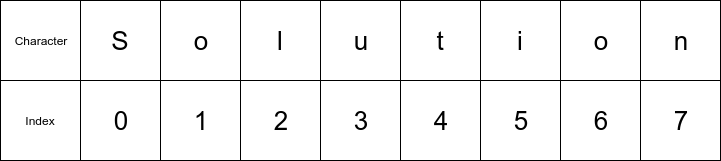
\includegraphics{images/string_indexing.png}
\caption{String index assignments}
\end{figure}
    




    
        \begin{lstlisting}[language=Python]
>>> word = 'Solution'
>>> word[0]
'S'
\end{lstlisting}
    




    
        \begin{lstlisting}[language=Python]
>>> word[1]
'o'
\end{lstlisting}
    




    
        \begin{lstlisting}[language=Python]
>>> word[7]
'n'
\end{lstlisting}
    




    
        If the eighth index of the word \passthrough{\lstinline!Solution!} is
called, an error is returned.

\begin{lstlisting}[language=Python]
>>> word[8]

IndexError: string index out of range
\end{lstlisting}
    




    
        \hypertarget{negative-indexing}{%
\subsubsection{Negative Indexing}\label{negative-indexing}}

Placing a negative number inside of the square brackets pulls a
character out of a string starting from the end of the string.

\begin{lstlisting}[language=Python]
>>> word[-1]
'n'
\end{lstlisting}

\begin{lstlisting}[language=Python]
>>> word[-2]
'o'
\end{lstlisting}

\begin{figure}
\centering
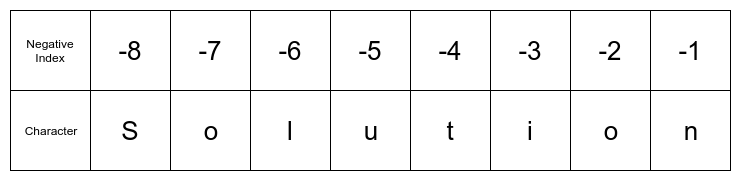
\includegraphics{images/reverse_string_indexing.png}
\caption{Negative string index assignments}
\end{figure}
    




    
        \hypertarget{string-slicing}{%
\subsection{String Slicing}\label{string-slicing}}

A colon on the inside of the square brackets between two numbers
indicates \emph{through}. If the index \passthrough{\lstinline![0:3]!}
is called, the characters at positions \passthrough{\lstinline!0!}
through \passthrough{\lstinline!3!} are returned. Remember Python
counting starts at \passthrough{\lstinline!0!} and ends at
\passthrough{\lstinline!n-1!}. So \passthrough{\lstinline![0:3]!}
indicates the first through third letters, which are indexes
\passthrough{\lstinline!0!} to \passthrough{\lstinline!2!}.

\begin{lstlisting}[language=Python]
>>> word[0:3]
'Sol'
\end{lstlisting}
    




    
        A colon by itself on the inside of square brackets indicates \emph{all}.

\begin{lstlisting}[language=Python]
>>> word[:]
'Solution'
\end{lstlisting}
    




    
        When three numbers are separated by two colons inside of square
brackets, the numbers represent \emph{start} : \emph{stop} :
\emph{step}. But remember that Python counting starts at
\passthrough{\lstinline!0!} and ends at \passthrough{\lstinline!n-1!}.

\begin{lstlisting}[language=Python]
>>> word[0:7:2]  #start:stop:step
'Slto'
\end{lstlisting}
    




    
        When two colons are used inside of square brackets, and less than three
numbers are specified, the missing numbers are set to their
``defaults''. The default start is \passthrough{\lstinline!0!}, the
default stop is \passthrough{\lstinline!n-1!}, and the default step is
\passthrough{\lstinline!1!}.

The two code lines below produce the same output since
\passthrough{\lstinline!0!} is the default start and
\passthrough{\lstinline!7!} (n-1) is the default stop. Both lines of
code use a step of \passthrough{\lstinline!2!}.

\begin{lstlisting}[language=Python]
>>> word[0:7:2]
'Slto'
\end{lstlisting}

\begin{lstlisting}[language=Python]
>>> word[::2]
'Slto'
\end{lstlisting}

The characters that make up a string can be reversed by using the
default start and stop values and specifying a step of
\passthrough{\lstinline!-1!}.

\begin{lstlisting}[language=Python]
>>> word[::-1]
'noituloS'
\end{lstlisting}
    



    \begin{Verbatim}[commandchars=\\\{\}]
{\color{incolor}In [{\color{incolor} }]:} 
\end{Verbatim}


    
        \hypertarget{print-statements}{%
\section{Print Statements}\label{print-statements}}
    




    
        The \passthrough{\lstinline!print()!} function useful in Python. The
value or expression inside of the parenthesis in the
\passthrough{\lstinline!print()!} function ``prints'' out to the REPL
when the \passthrough{\lstinline!print()!} function is called.

An example using the \passthrough{\lstinline!print()!} function is
below:

\begin{lstlisting}[language=Python]
>>> name = "Gabby"
>>> print("Your name is: ")
Your name is
>>> print(name)
Gabby
\end{lstlisting}

Remember that strings must be enclosed by quotation marks. The following
command produces an error.

\begin{lstlisting}[language=Python]
>>> print(Gabby)

NameError: name 'Gabby' is not defined
\end{lstlisting}

This error is corrected by surrounding the string
\passthrough{\lstinline!Gabby!} with quotation marks.

\begin{lstlisting}[language=Python]
>>> print("Gabby")
Gabby
\end{lstlisting}
    




    
        Expressions passed to the \passthrough{\lstinline!print()!} function are
evaluated before they are printed out. For instance, the sum of two
numbers can be shown with the \passthrough{\lstinline!print()!}
function.

\begin{lstlisting}[language=Python]
>>>print(1+2)
3
\end{lstlisting}

If you want to see the text \passthrough{\lstinline!1+2!}, you need to
define \passthrough{\lstinline!"1+2"!} as a string and print out the
string \passthrough{\lstinline!"1+2"!} instead.

\begin{lstlisting}[language=Python]
>>>print("1+2")
1+2
\end{lstlisting}
    




    
        Strings can be concatenated (combined) inside of a
\passthrough{\lstinline!print()!} statement.

\begin{lstlisting}[language=Python]
>>> name = Gabby
>>> print('Your name is: ' + name)
Your name is Gabby
\end{lstlisting}
    




    
        The \passthrough{\lstinline!print()!} function also prints out
individual expressions one after another with a space in between when
the expressions are placed inside the \passthrough{\lstinline!print()!}
function and separated by a comma.

\begin{lstlisting}[language=Python]
>>> print("Name:","Gabby","Age", 3+5)
Name: Gabby Age 8
\end{lstlisting}
    



    \begin{Verbatim}[commandchars=\\\{\}]
{\color{incolor}In [{\color{incolor} }]:} 
\end{Verbatim}


    
        \newpage
        \hypertarget{summary}{%
\section{Summary}\label{summary}}

    




    
        In this chapter, you learned how to use the Python REPL, also called the
Python prompt, to solve calculation problems. You learned how to do
arithmetic, powers and logarithms, trigonometry and save values to
variables. Operations on strings were introduced including
concatenation, comparison, indexing, and slicing. In the last section of
the chapter, Python's \passthrough{\lstinline!print()!} function was
introduced. As shown multiple times through this chapter, remember
Python counting starts at \passthrough{\lstinline!0!} and ends at
\passthrough{\lstinline!n-1!}.
    




    
        \begin{key_terms}
        \hypertarget{key-terms-and-concepts}{%
\subsection{Key Terms and Concepts}\label{key-terms-and-concepts}}

REPL

Python REPL

Python Prompt

prompt

Python Interpreter

interpreter

operator

mathematical operator

import

module

Python Standard Library

Standard Library

syntax

functions

command line

error

variable

assignment operator

comparison operator

concatenate

equivalent

index

indexing

slicing
        \end{key_terms}

    




    
        \hypertarget{summary-of-python-functions-and-commands}{%
\subsection{Summary of Python Functions and
Commands}\label{summary-of-python-functions-and-commands}}

Below is a summary of the functions and operators used in this chapter:

\hypertarget{arithmetic}{%
\subsubsection{Arithmetic}\label{arithmetic}}

\begin{longtable}[]{@{}ll@{}}
\toprule
Arithmetic Operators & Description\tabularnewline
\midrule
\endhead
\passthrough{\lstinline!+!} & addition\tabularnewline
\passthrough{\lstinline!-!} & subtraction\tabularnewline
\passthrough{\lstinline!*!} & multiplication\tabularnewline
\passthrough{\lstinline!/!} & division\tabularnewline
\passthrough{\lstinline!**!} & exponents\tabularnewline
\passthrough{\lstinline!\_!} & answer in memory\tabularnewline
\bottomrule
\end{longtable}

\hypertarget{trigonometry}{%
\subsubsection{Trigonometry}\label{trigonometry}}

\begin{longtable}[]{@{}ll@{}}
\toprule
Trig Function & Description\tabularnewline
\midrule
\endhead
\passthrough{\lstinline!from math import *!} &\tabularnewline
\passthrough{\lstinline!sin!} & sine of angle in radians\tabularnewline
\passthrough{\lstinline!cos!} & cosine of angle in
radians\tabularnewline
\passthrough{\lstinline!tan!} & tangent of angle in
radians\tabularnewline
\passthrough{\lstinline!pi!} & \(\pi\)\tabularnewline
\passthrough{\lstinline!degrees!} & convert radians to
degrees\tabularnewline
\passthrough{\lstinline!radians!} & convert degrees to
radians\tabularnewline
\passthrough{\lstinline!asin!} & inverse sine\tabularnewline
\passthrough{\lstinline!acos!} & inverse cosine\tabularnewline
\passthrough{\lstinline!atan!} & inverse tangent\tabularnewline
\bottomrule
\end{longtable}

\hypertarget{logarithms-and-exponents}{%
\subsubsection{Logarithms and
Exponents}\label{logarithms-and-exponents}}

\begin{longtable}[]{@{}ll@{}}
\toprule
Logarithms and Exponent Function & Description\tabularnewline
\midrule
\endhead
\passthrough{\lstinline!from math import *!} &\tabularnewline
\passthrough{\lstinline!log!} & log base e, natural log\tabularnewline
\passthrough{\lstinline!log10!} & log base 10\tabularnewline
\passthrough{\lstinline!exp!} & \(e^{power}\)\tabularnewline
\passthrough{\lstinline!e!} & the math constant \(e\)\tabularnewline
\passthrough{\lstinline!pow(x,y)!} & x raised to the y
power\tabularnewline
\passthrough{\lstinline!sqrt!} & square root\tabularnewline
\bottomrule
\end{longtable}

\hypertarget{statistics}{%
\subsubsection{Statistics}\label{statistics}}

\begin{longtable}[]{@{}ll@{}}
\toprule
Statistical Function & Description\tabularnewline
\midrule
\endhead
\passthrough{\lstinline!from statistics import *!} &\tabularnewline
\passthrough{\lstinline!mean!} & mean (average)\tabularnewline
\passthrough{\lstinline!median!} & median (middle value)\tabularnewline
\passthrough{\lstinline!mode!} & (most often)\tabularnewline
\passthrough{\lstinline!stdev!} & standard deviation of a
sample\tabularnewline
\passthrough{\lstinline!pstdev!} & standard deviation of a
population\tabularnewline
\bottomrule
\end{longtable}
    



    \begin{Verbatim}[commandchars=\\\{\}]
{\color{incolor}In [{\color{incolor} }]:} 
\end{Verbatim}


    
        \hypertarget{review-questions}{%
\section{Review Questions}\label{review-questions}}
    




    
        \begin{problems}
        \hypertarget{arithmetic}{%
\subsubsection{Arithmetic}\label{arithmetic}}

Q02.01 \(2 + \frac{1}{2}\)

Q02.02 \(4 \times 2 + \frac{2}{4}\)

Q02.03 \(\frac{5}{2} \times 3 + 4\)

Q02.04 \(4^2 + 3\)

Q02.05 \(\sqrt{16}\)

Q02.06 \(3^{4-5}\)

Q02.07 \(\frac{1+3+5}{2+4+6}\)

Q02.08 \(1 - 2 + \frac{9}{6} -3 + 5\)

Q02.09 \((3 + 5 -2)^{2/3}\)

Q02.10 \(\frac{5+3}{2 \times 5}\)

Q02.11 \(\sqrt{6^2 + 4}\)

Q02.12 \(1 + 9 \times \frac{8}{4^2} + 1^{3-4} \times \frac{1}{2.5}\)
        \end{problems}

    




    
        \hypertarget{string-indexing}{%
\subsubsection{String Indexing}\label{string-indexing}}

Q02.15 Write two lines of code that pulls out the first three letters of
the word ``Problem''

Q02.16 Write two lines of code that pulls out the last four letters of
the word ``Problem''

Q02.17 Write two lines of code that pulls out every other letter of the
word ``Problem'' starting with the letter ``P''.

Q02.18 Write two lines of code that rewrites the word ``Problem''
backwards
    




    
        \begin{problems}
        \hypertarget{trigonometry}{%
\subsubsection{Trigonometry}\label{trigonometry}}

Q2.30 Find the sine of \(0\), \(\pi/4\), \(\pi/2\), \(3\pi/4\), and
\(\pi\).

Q2.31 Find the cosine of 0 degrees, 30 degrees, 60 degrees and 90
degrees.

Q2.32 Find the tangent of 3/4, 5/12, and -8/6.

Q2.33 Find the sin of 0.1 radians. Then find the arcsine of the result
and see if it equals 0.1 radians.

Q02.34 The U.S. Forest service can use trigonometry to find the height
of trees. The height of a tree, \(h\) is equal to the distance \(d\)
between an observer and the base of the tree multiplied by the tangent
of the angle \(\theta\) between looking straight along the ground and
looking up at the top of tree according to the formula:

\[ h = d\tan(\theta) \]

If a Forest Service ranger is 20 feet away from the base of a douglas
fir tree and looks up at a 63 degree angle relative to straight ahead to
see the top of the tree, what is the height of the douglas fir tree?

Q02.35 The tangent of an angle is equal to the sine of the angle divided
by the cosine of the angle. Make two calculations, one for the tangent
of -29 degrees and another calculation for the sine of -29 degrees
divided by the cosine of -29 degrees. Do you observe the output of both
calculations to be the same?

Q02.36 A simple model of water level based on tides (assuming high tide
is at midnight) is:

\[ h = (4.8)\sin(\pi/6)(t+3)+5.1 \]

Where \(h\) is the water height and \(t\) is the number of hours since
midnight. Using this model, calculate the water level \(h\) at 6am
(\(t=6\) hours since midnight).

Q02.37 The x-component of a force \(F_x\) is equal to the magnitude of
the force \(|\vec{F}|\) multiplied by the cosine of the angle \(\theta\)
of the force relative to the positive x-axis.

\[ F_x = |\vec{F}|\cos(\theta) \]

If the magnitude of a force \(|\vec{F}| = 12.4\) and the force acts at
\(\theta=110\) degrees relative to the positive x-axis, what is the
x-component of the force \(F_x\)?

Q02.37 The distance \(d\) a free-thrown projectile travels is dependent
on the projectile's initial velocity \(v_0\), the acceleration due to
gravity \(g=9.81 m/s^2\) and the angle \(\theta\) at which the project
is launched according to:

\[ d = \frac{{v_0}^2}{g} \sin(2\theta) \]

If a projectile is launched at a 12 degree angle with an initial
velocity of 150 m/s, how far will the projectile travel?

Q02.38 A problem with sin and AC current
        \end{problems}

    




    
        \begin{problems}
        \hypertarget{logarithms-and-exponents}{%
\subsubsection{Logarithms and
Exponents}\label{logarithms-and-exponents}}

Q02.41 Show that the natural log of Euler's number, \(\ln(e)\), is equal
to one.

Q02.42 Logarithms turn multiplication into addition. Complete both of
the calculations below to see if the expressions are equal to each
other:

\[ \log(87.1 \times 210 \times 10^{3}) \]

\[ \log(87.1) + \log(210) + \log(10^{3}) \]

Q02.43 Logarithms turn exponents into multiplication. Complete both of
the calculations below to see if the expressions are equal.

\[ \log(6.02 \times 10^{23}) \]

\[ (23)\log(6.02) \]

Q02.44 Python's math module has the natural log (\(\ln\)) function
\passthrough{\lstinline!math.log()!} and the log (base 10) function
\passthrough{\lstinline!math.log10()!}. If you want to find the log with
an arbitrary base, \(b\), of a number \(n\), you can use a ratio of
natural logarithms (log base \(e\)) according to:

\[ \log_b(n) = \frac{\ln(n)}{\ln(b)} \]

Calculate the base 4 logarithm of \(3.9 \times 10^{-9}\)

\[ log_{4}(3.9 \times 10^{-9}) \]

Q02.45 The magnitude of a vector \(|\vec{v}|\) is equal to the square
root of the sum of the squares of the vector's components \(v_x\),
\(v_y\), and \(v_z\) according to:

\[ |\vec{v}| = \sqrt{{v_x}^2 + {v_y}^2 + {v_z}^2} \]

What is the magnitude of a vector \(\vec{v}\) that has components
\(v_x = 76.3\), \(v_y = 70.9\), \(v_z = 93.6\) ?

Q02.46 Moore's Law, a relationship that states the number of transistors
that fit on a microchip doubles every two years can be modeled as:

\[ P_n = P_0 \times 2^n \]

Where \(P_0\) is the original number of transistors on a microchip and
\(P_n\) is the number of transistors on a microchip after \(n\) number
of years since the original microchip. If the original microchip has
1000 transistors, how many transistors were projected to be on a
microchip 40 years later?
        \end{problems}

    




    
        \begin{problems}
        \hypertarget{variables-in-calculations}{%
\subsubsection{Variables in
Calculations}\label{variables-in-calculations}}

Q02.71 \(a = 2\), \(b = 3\), calculate \(\frac{4}{5}(a^2 - b^3)\)

Q02.72 The area of a circle, \(a\), is dependent on the circle's radius,
\(r\), according to \(a=\pi r^2\). What is the area of a circle with
radius \(r=4\)?

Q02.73 The area of a circle, \(a\), is dependent on the circle's
diameter, \(d\), according to \(a=\pi (\frac{d}{2})^2\). What is the
area of a circle with diameter \(d=6\)?

Q02.74 The volume of a sphere, \(v\), is dependent on the sphere's
radius, \(r\), according to \(v=(\frac{4}{3})\pi r^3\). What is the
volume of a sphere with radius \(r=1.5\)?

Q02.75 The volume of a cylinder, \(v\), is dependent on the cylinder's
radius, \(r\), and height, \(h\), according to \(v=\pi r^2 h\). What is
the volume of a cylinder with radius \(r=5\) and height \(h=10\) ?

Q02.76 The surface area of a sphere, \(a_s\) is related to the sphere's
radius, \(r\), according to \(a_s=4\pi r^2\). What is the surface area
\(a_s\) of a sphere with radius \(r=2.5\)?

Q02.77 The general equation for the distance, \(d\), that a free falling
body travels (neglecting air resistance) is \(d = \frac{1}{2}gt^2\),
where \(g\) is the acceleration due to gravity and \(t\) is the fall
time. Assume the acceleration due to gravity \(g = 9.81\). How far (what
distance) will a ball fall in time \(t = 12\)?

Q02.78 The general equation for the fall time, \(t\), that a free
falling body takes (neglecting air resistance) to cover a distance,
\(d\) is \(t = \sqrt{\frac{d}{0.5g}}\), where \(g\) is the acceleration
due to gravity. Assume the acceleration due to gravity \(g = 9.81\). How
long (what time) will it take a base jumper to fall distance
\(d = 2000\)?

Q02.79 The value of an investment \(v\) compounded annually at an
interest rate of \(r\%\) after \(n\) years is dependent on the original
investment \(P\) according to:

\[ v = P(1 + r/100)^n \]

If \(P=1000\) dollars at a rate of \(r=7\%\), what will the value \(v\)
be after \(n=20\) years?

Q02.80 The original principal \(P\) needed to produce a total savings of
value \(v\) at a rate of \(r\%\) over \(n\) years is calculated by:

\[ P = \frac{v}{(1+r/100)^n} \]

What is the principal \(P\) needed to save one million dollars at a rate
\(r=10\%\) over \(n=40\) years?

Q02.81 Electrical power \(P\) is related to current \(I\) and resistance
\(R\) according to \(P = I^2R\). An electrical load with a resistance
\(R = 10,000\) running at a current \(I=0.200\) draws how much power
\(P\) ?
        \end{problems}

    




    
        \hypertarget{errors-explanations-and-solutions}{%
\subsubsection{Errors, Explanations, and
Solutions}\label{errors-explanations-and-solutions}}

For each of the problems below, run the line of code. Then explain the
error in your words. Give an explanation more specific than
\passthrough{\lstinline!invalid syntax!}. Then suggest and run a line of
code that fixes the error.

Q02.91

\begin{lstlisting}[language=Python]
>>> 9 x 10
\end{lstlisting}

Q02.92

\begin{lstlisting}[language=Python]
>>> 1 1/2 + 2 2/3
\end{lstlisting}

Q02.93

\begin{lstlisting}[language=Python]
>>> 3cos(35)
\end{lstlisting}

Q02.94

\begin{lstlisting}[language=Python]
>>> 8.31 x 10^9
\end{lstlisting}

Q02.95

\begin{lstlisting}[language=Python]
>>> (2+3)**(2-3e(4)
\end{lstlisting}

Q02.96

\begin{lstlisting}[language=Python]
>>> 7% + 8% + 9%
\end{lstlisting}

Q02.97

\begin{lstlisting}[language=Python]
>>> (-)54.2 + 9.2
\end{lstlisting}

Q02.98

\begin{lstlisting}[language=Python]
>>> '5' / '4'
\end{lstlisting}

Q02.99

\begin{lstlisting}[language=Python]
>>> ln(e) - log(10)
\end{lstlisting}
    



    \begin{Verbatim}[commandchars=\\\{\}]
{\color{incolor}In [{\color{incolor} }]:} 
\end{Verbatim}


    
        \hypertarget{data-types-and-variables}{%
\chapter{Data Types and Variables}\label{data-types-and-variables}}
    




    
        \hypertarget{introduction}{%
\section{Introduction}\label{introduction}}
        \newpage



    




    
        Python has many built-in data types. These include integers, floats,
booleans, strings, and lists.

By the end of this chapter you will be able to:

\begin{itemize}
\item
  Explain the difference between Python's built-in data types
\item
  Define variables with the assignment operator
  \passthrough{\lstinline!=!}
\item
  Create variables with different data types
\item
  Use Python's \passthrough{\lstinline!type()!} function to determine an
  object's type
\item
  Complete logical evaluations of variables
\item
  Convert variables from one data type to another
\end{itemize}
        \newpage



    



    \begin{Verbatim}[commandchars=\\\{\}]
{\color{incolor}In [{\color{incolor} }]:} 
\end{Verbatim}


    
        \hypertarget{numeric-data-types}{%
\section{Numeric Data Types}\label{numeric-data-types}}
    




    
        Python has many useful built-in data types. Python variables can store
different types of data. A variable's data type is created dynamically,
without the need to explicitly define a data type when the variable is
created.

It is useful for problem solvers to understand a couple of Python's core
data types in order to write well-constructed code.

\hypertarget{a-review-of-variable-assignment-in-python}{%
\subsection{A review of variable assignment in
Python}\label{a-review-of-variable-assignment-in-python}}

Remember from the previous chapter that variables in Python are defined
with the assignment operator, the equals sign
\passthrough{\lstinline!=!}. Recall that to define a variable in Python,
the variable name is written first, then the assignment operator
\passthrough{\lstinline!=!} followed by a value or expression.

The general syntax to assign a value to variable name is below:

\begin{lstlisting}
variable_name = value
\end{lstlisting}

Variable names in Python must adhere to the following rules:

\begin{itemize}
\tightlist
\item
  variable names must start with a letter
\item
  variable names can only contain letters, numbers and the underscore
  character \passthrough{\lstinline!\_!}
\item
  variable names can not contain spaces
\item
  variable names are not enclosed in quotes or brackets
\end{itemize}

Below is a discussion of a few different built-in data types in Python.
    




    
        \hypertarget{integers}{%
\subsection{Integers}\label{integers}}

\emph{Integers} are one of the Python data types. An integer is a whole
number, negative, positive or zero. In Python, integer variables are
defined by simply assigning a whole number to a variable. Python's
\passthrough{\lstinline!type()!} function can be used to determine the
data type of a variable.

\begin{lstlisting}[language=Python]
>>> a = 5
>>> type(a)
<class 'int'>
\end{lstlisting}

The output \passthrough{\lstinline!<class 'int'>!} indicates the
variable \passthrough{\lstinline!a!} is an integer. Integers can be
negative or zero.

\begin{lstlisting}[language=Python]
>>> b = -2
>>> type(b)
<class 'int'>
>>> z = 0
>>> type(z)
<class 'int'>
\end{lstlisting}
    




    
        \hypertarget{floating-point-numbers}{%
\subsection{Floating Point Numbers}\label{floating-point-numbers}}

Floating point numbers or \emph{floats} are another Python data type.
Floats are decimals, positive, negative and zero. Floats can also be
numbers in scientific notation which contain exponents.

Both a lower case \passthrough{\lstinline!e!} or an upper case
\passthrough{\lstinline!E!} can be used to define floats in scientific
notation. In Python, a float can be defined using a decimal point
\passthrough{\lstinline!.!} when a variable is assigned.

\begin{lstlisting}[language=Python]
>>> c = 6.2
>>> type(c)
<class 'float'>
>>> d = -0.03
>>> type(d)
<class 'float'>
>>> Na = 6.02e23
>>> Na
6.02e+23
>>> type(Na)
<class 'float'>
\end{lstlisting}

To define a variable as a float instead of an integer, even if the
variable is assigned a whole number, a trailing decimal point
\passthrough{\lstinline!.!} is used. Note the difference when a decimal
point \passthrough{\lstinline!.!} comes after a whole number:

\begin{lstlisting}[language=Python]
>>> g = 5
>>> type(g)
<class 'int'>
>>> g = 5.
>>> type(g)
<class 'float'>
\end{lstlisting}
    




    
        \hypertarget{complex-numbers}{%
\subsection{Complex Numbers}\label{complex-numbers}}

Another useful numeric data type for problem solvers is the
\emph{complex number} data type. A complex number is defined in Python
using a real component \passthrough{\lstinline!+!} an imaginary
component \passthrough{\lstinline!j!}. The letter
\passthrough{\lstinline!j!} must be used to denote the imaginary
component. Using the letter \passthrough{\lstinline!i!} to define a
complex number in Python returns an error. Note how imaginary numbers
add to integers and floats.

\begin{lstlisting}[language=Python]
>>> comp = 4 + 2j
>>> type(comp)
<class 'complex'>

>>> comp2 = 4 + 2i
              ^
SyntaxError: invalid syntax
\end{lstlisting}

\begin{lstlisting}[language=Python]
>>> intgr = 3
>>> type(intgr)
<class 'int'>

>>> comp_sum = comp + intgr
>>> print(comp_sum)
(7+2j)

>>> flt = 2.1
>>> comp_sum = comp + flt
>>> print(comp_sum)
(6.1+2j)
\end{lstlisting}
    



    \begin{Verbatim}[commandchars=\\\{\}]
{\color{incolor}In [{\color{incolor} }]:} 
\end{Verbatim}


    
        \hypertarget{boolean-data-type}{%
\section{Boolean Data Type}\label{boolean-data-type}}
    




    
        The \emph{boolean} data type is either True or False. In Python, boolean
variables are defined by the \passthrough{\lstinline!True!} and
\passthrough{\lstinline!False!} keywords.

\begin{lstlisting}[language=Python]
>>> a = True
>>> type(a)
<class 'bool'>

>>> b = False
>>> type(b)
<class 'bool'>
\end{lstlisting}

The output \passthrough{\lstinline!<class 'bool'>!} indicates the
variable is a boolean data type.

Note that \passthrough{\lstinline!True!} and
\passthrough{\lstinline!False!} must have an Upper Case first letter.
Using a lowercase \passthrough{\lstinline!true!} returns an error.

\begin{lstlisting}[language=Python]
>>> c = true
Traceback (most recent call last):
  File "<input>", line 1, in <module>
NameError: name 'true' is not defined
   
>>> d = false
Traceback (most recent call last):
  File "<input>", line 1, in <module>
NameError: name 'false' is not defined
\end{lstlisting}
    




    
        \hypertarget{integers-and-floats-as-booleans}{%
\subsection{Integers and Floats as
Booleans}\label{integers-and-floats-as-booleans}}

Integers and floating point numbers can be converted to the boolean data
type using Python's \passthrough{\lstinline!bool()!} function. An int,
float or complex number set to zero returns as
\passthrough{\lstinline!False!}. An integer, float or complex number set
to any other number, positive or negative, returns as
\passthrough{\lstinline!True!}.

\begin{lstlisting}[language=Python]
>>> zero_int = 0
>>> bool(zero_int)
False
\end{lstlisting}

\begin{lstlisting}[language=Python]
>>> pos_int = 1
>>> bool(pos_int)
True
\end{lstlisting}

\begin{lstlisting}[language=Python]
>>> neg_flt = -5.1
>>> bool(neg_flt)
True
\end{lstlisting}
    




    
        \hypertarget{boolean-arithmetic}{%
\subsection{Boolean Arithmetic}\label{boolean-arithmetic}}

\emph{Boolean arithmetic} is the arithmetic of true and false logic. A
boolean or logical value can either be \passthrough{\lstinline!True!} or
\passthrough{\lstinline!False!}. Boolean values can be manipulated and
combined with \emph{boolean operators}. Boolean operators include
\passthrough{\lstinline!and!}, \passthrough{\lstinline!or!}, and
\passthrough{\lstinline!not!}.

The common boolean operators in Python are below:

\begin{itemize}
\tightlist
\item
  \passthrough{\lstinline!or!}
\item
  \passthrough{\lstinline!and!}
\item
  \passthrough{\lstinline!not!}
\item
  \passthrough{\lstinline!==!} (equivalent)
\item
  \passthrough{\lstinline"!="} (not equivalent)
\end{itemize}

In the code section below, two variables are assigned the boolean values
\passthrough{\lstinline!True!} and \passthrough{\lstinline!False!}. Then
these boolean values are combined and manipulated with boolean
operators.

\begin{lstlisting}[language=Python]
>>> A = True
>>> B = False
\end{lstlisting}

\begin{lstlisting}[language=Python]
>>> A or B
True
\end{lstlisting}

\begin{lstlisting}[language=Python]
>>> A and B
False
\end{lstlisting}

\begin{lstlisting}[language=Python]
>>> not A
False
\end{lstlisting}

\begin{lstlisting}[language=Python]
>>> not B
True
\end{lstlisting}

\begin{lstlisting}[language=Python]
>>> A == B
False
\end{lstlisting}

\begin{lstlisting}[language=Python]
>>> A != B
True
\end{lstlisting}

Boolean operators such as \passthrough{\lstinline!and!},
\passthrough{\lstinline!or!}, and \passthrough{\lstinline!not!} can be
combined with parenthesis to make compound \emph{boolean expressions}.

\begin{lstlisting}[language=Python]
>>> C = False
>>> A or (C and B)
True
>>> (A and B) or C
False
\end{lstlisting}
    




    
        A summary of boolean arithmetic and boolean operators is shown in the
table below:

\begin{longtable}[]{@{}llllllll@{}}
\toprule
A & B & not A & not B & A == B & A =! B & A or B & A and
B\tabularnewline
\midrule
\endhead
T & F & F & T & F & T & T & F\tabularnewline
F & T & T & F & F & T & T & F\tabularnewline
T & T & F & F & T & F & T & T\tabularnewline
F & F & T & T & T & F & F & F\tabularnewline
\bottomrule
\end{longtable}
    



    \begin{Verbatim}[commandchars=\\\{\}]
{\color{incolor}In [{\color{incolor} }]:} 
\end{Verbatim}


    
        \hypertarget{strings}{%
\section{Strings}\label{strings}}
    




    
        Another built-in Python data type is \emph{strings}. Strings are
sequences of letters, numbers, symbols, and spaces. In Python, strings
can be almost any length and can contain spaces. String variables are
assigned in Python using quotation marks \passthrough{\lstinline!'   '!}
or \passthrough{\lstinline!" "!}. In Python, strings can be defined by
single quotation marks \passthrough{\lstinline!' '!} or double quotation
marks \passthrough{\lstinline!" "!}.

Python strings can contain blank spaces. A blank space is a valid
character in Python string.

\begin{lstlisting}[language=Python]
>>> string = 'z'
>>>> type(string)
<class 'str'>

>>> string = 'Engineers'
>>> type(string)
<class 'str'>
\end{lstlisting}

The output \passthrough{\lstinline!<class 'str'>!} indicates the
variable is a string.
    




    
        \hypertarget{numbers-as-strings}{%
\subsection{Numbers as Strings}\label{numbers-as-strings}}

Numbers and decimals can be defined as strings too. If a decimal number
is defined using quotes \passthrough{\lstinline!'   '!}, the number is
saved as a string rather than as a float. Integers defined using quotes
will become strings as well if surrounded by quotes.

\begin{lstlisting}[language=Python]
>>> num = '5.2'
>>> type(num)
<class 'str'>

>>> num = '2'
>>> type(num)
<class 'str'>
\end{lstlisting}
    




    
        \hypertarget{strings-as-boolean-values}{%
\subsection{Strings as Boolean Values}\label{strings-as-boolean-values}}

Strings can be converted to boolean values (converted to True or False).
The empty string \passthrough{\lstinline!""!} returns as
\passthrough{\lstinline!False!}. All other strings convert to
\passthrough{\lstinline!True!}.

\begin{lstlisting}[language=Python]
>>> name = "Gabby"
>>> bool(name)
True
\end{lstlisting}

\begin{lstlisting}[language=Python]
>>> empty = ""
>>> bool(empty)
False
\end{lstlisting}

Note that a string which contains just one space
(\passthrough{\lstinline!" "!}) is not empty. It contains the space
character. Therefore a string made up of just one space converts to
\passthrough{\lstinline!True!}.

\begin{lstlisting}[language=Python]
>>> space = " "
>>> bool(space)
True
\end{lstlisting}
    



    \begin{Verbatim}[commandchars=\\\{\}]
{\color{incolor}In [{\color{incolor} }]:} 
\end{Verbatim}


    
        \hypertarget{lists}{%
\section{Lists}\label{lists}}
    




    
        A list is a data structure in Python that can contain multiple elements
of any of the other data type. A list is defined with square brackets
\passthrough{\lstinline![ ]!} and commas \passthrough{\lstinline!,!}
between elements.

\begin{lstlisting}[language=Python]
>>> lst = [ 1, 2, 3 ]
>>> type(lst)
list

>>> lst = [ 1, 5.3, '3rd_Element']
>>> type(lst)
list
\end{lstlisting}
    




    
        \hypertarget{indexing-lists}{%
\subsection{Indexing Lists}\label{indexing-lists}}

Individual elements of a list can be accessed or \emph{indexed} using
bracket \passthrough{\lstinline![ ]!} notation. Note that Python lists
start with the index zero, not the index 1. For example:

\begin{lstlisting}[language=Python]
>>> lst = ['statics', 'strengths', 'dynamics']
>>> lst[0]
'statics'

>>> lst[1]
'strengths'

>>> lst[2]
'dynamics'
\end{lstlisting}

Remember! Python lists start indexing at {[}0{]} not at {[}1{]}. To call
the elements in a list with 3 values use: lst{[}0{]}, lst{[}1{]},
lst{[}2{]}.

Colons \passthrough{\lstinline!:!} are used inside the square brackets
to denote \emph{all}

\begin{lstlisting}[language=Python]
>>> lst = [2, 4, 6]
>>> lst[:]
[2, 4, 6]
\end{lstlisting}

Negative numbers can be used as indexes to call the last number of
elements in the list

\begin{lstlisting}[language=Python]
>>> lst = [2, 4, 6]
>>> lst[-1]
6
\end{lstlisting}

The colon operator can also be used to denote \emph{all upto} and
\emph{from thru end}.

\begin{lstlisting}[language=Python]
>>> lst = [2, 4, 6]
>>> lst[:2]
[2, 4]



lst = [2, 4, 6]
lst[2:]
[6]
\end{lstlisting}

The colon operator can also be used to denote \emph{start : end + 1}.
Note that the indexing here in not inclusive.
\passthrough{\lstinline!lst[1:3]!} will return the 2nd element, and 3rd
element but not the fourth even though \passthrough{\lstinline!3!} is
used in the index.

Remember! Python indexing is not inclusive. The last element called in
an index will not be returned.
    



    \begin{Verbatim}[commandchars=\\\{\}]
{\color{incolor}In [{\color{incolor} }]:} 
\end{Verbatim}


    
        \hypertarget{dictionaries-and-tuples}{%
\section{Dictionaries and Tuples}\label{dictionaries-and-tuples}}
    




    
        Besides lists, Python has two additional data structures that can store
multiple objects. These data structures are \emph{dictionaries} and
\emph{tuples}.
    




    
        \hypertarget{dictionaries}{%
\subsection{Dictionaries}\label{dictionaries}}
    




    
        Dictionaries are made up of key: value pairs. In Python, lists are
organized and accessed based on position. Dictionaries in Python are
organized and accessed using keys and values. The location of a pair of
keys and values stored in a Python dictionary is irrelevant.

Dictionaries are defined in Python with curly braces
\passthrough{\lstinline!\{  \}!}. Commas separate the key-value pairs
that make up the dictionary. Each key-value pair is related by a colon
\passthrough{\lstinline!:!}.

Let's store the ages of two people in a dictionary. The two people are
\passthrough{\lstinline!Gabby!} and \passthrough{\lstinline!Maelle!}.
\passthrough{\lstinline!Gabby!} is \passthrough{\lstinline!8!} and
\passthrough{\lstinline!Maelle!} is \passthrough{\lstinline!5!}. Note
the name \passthrough{\lstinline!Gabby!} is a string and the age
\passthrough{\lstinline!8!} is an integer.

\begin{lstlisting}[language=Python]
>>> age_dict = {"Gabby": 8 , "Maelle": 5}
>>> type(age_dict)
dict
\end{lstlisting}

The values stored in a dictionary are called and assigned using the
following syntax:

\begin{lstlisting}[language=Python]
dict_name[key] = value
\end{lstlisting}

\begin{lstlisting}[language=Python]
>>> age_dict = {"Gabby": 8 , "Maelle": 5}
>>> age_dict["Gabby"]
8
\end{lstlisting}

We can add a new person to our \passthrough{\lstinline!age\_dict!} with
the following command:

\begin{lstlisting}[language=Python]
>>> age_dict = {"Gabby": 8 , "Maelle": 5}

>>> age_dict["Peter"]= 40
>>> age_dict
{'Gabby': 8, 'Maelle': 5, 'Peter': 40}
\end{lstlisting}

Dictionaries can be converted to lists by calling the
\passthrough{\lstinline!.items()!}, \passthrough{\lstinline!.keys()!},
and \passthrough{\lstinline!.values()!} methods.

\begin{lstlisting}[language=Python]
>>> age_dict = {"Gabby": 8 , "Maelle": 5}

>>> whole_list = list(age_dict.items())
>>> whole_list
[('Gabby', 8), ('Maelle', 5)]

>>> name_list = list(age_dict.keys())
>>> name_list
['Gabby', 'Maelle']

>>> age_list = list(age_dict.values())
>>> age_list
[8, 5]
\end{lstlisting}
    




    
        \hypertarget{tuples}{%
\subsection{Tuples}\label{tuples}}
    




    
        Tuples are immutable lists. Elements of a list can be modified, but
elements in a tuple can only be accessed, not modified. The name
\emph{tuple} does not mean that only two values can be stored in this
data structure.

Tuples are defined in Python by enclosing elements in parenthesis
\passthrough{\lstinline!( )!} and separating elements with commas. The
command below creates a tuple containing the numbers
\passthrough{\lstinline!3!}, \passthrough{\lstinline!4!}, and
\passthrough{\lstinline!5!}.

\begin{lstlisting}[language=Python]
>>> t_var = (1,2,3)
>>> t_var
(1, 2, 3)
\end{lstlisting}

Note how the elements of a list can be modified:

\begin{lstlisting}[language=Python]
>>> l_var = [3,4,5]  # a list
>>> l_var[0]= 8
>>> l_var
[8, 4, 5]
\end{lstlisting}

The elements of a tuple can not be modified. If you try to assign a new
value to one of the elements in a tuple, an error is returned.

\begin{lstlisting}[language=Python]
>>> t_var = (3,4,5)  # a tuple
>>> t_var[0]= 8
>>> t_var

TypeError: 'tuple' object does not support item assignment
\end{lstlisting}

To create a tuple that just contains one numerical value, the number
must be followed by a comma. Without a comma, the variable is defined as
a number.

\begin{lstlisting}[language=Python]
>>> num = (5)
>>> type(num)
int
\end{lstlisting}

When a comma is included after the number, the variable is defined as a
tuple.

\begin{lstlisting}[language=Python]
>>> t_var = (5,)
>>> type(t_var)
tuple
\end{lstlisting}
    



    \begin{Verbatim}[commandchars=\\\{\}]
{\color{incolor}In [{\color{incolor} }]:} 
\end{Verbatim}


    
        \newpage
        \hypertarget{summary}{%
\section{Summary}\label{summary}}

    




    
        In this chapter, we reviewed a couple of different data types built-in
to Python. These data types include the numeric data types: integers,
floats, and complex numbers. The string data type is composed of
letters, numbers, spaces, and punctuation. Python also has container
data types which can store many values. These container data types are
lists, tuples, and dictionaries.
    




    
        \hypertarget{key-terms-and-concepts}{%
\subsection{Key Terms and Concepts}\label{key-terms-and-concepts}}
    




    
        \begin{key_terms}
        data type

variable

assignment operator

integer

int

whole number

floating point number

float

scientific notation

complex number

string

boolean

bool

boolean arithmetic

boolean operators

or

and

not

data structure

dictionary

tuple

list

index

indexing
        \end{key_terms}

    




    
        \hypertarget{summary-of-python-functions-and-commands}{%
\subsection{Summary of Python Functions and
Commands}\label{summary-of-python-functions-and-commands}}
    




    
        \hypertarget{built-in-data-types}{%
\subsubsection{Built-in Data Types}\label{built-in-data-types}}

\begin{longtable}[]{@{}ll@{}}
\toprule
Python Object & Description\tabularnewline
\midrule
\endhead
\passthrough{\lstinline!int!} & integer\tabularnewline
\passthrough{\lstinline!float!} & floating point number\tabularnewline
\passthrough{\lstinline!bool!} & boolean value: True or
False\tabularnewline
\passthrough{\lstinline!complex!} & complex number, real and imaginary
components\tabularnewline
\passthrough{\lstinline!str!} & string, sequence of letters, numbers and
symbols\tabularnewline
\passthrough{\lstinline!list!} & a Python list\tabularnewline
\passthrough{\lstinline!dict!} & a Python dictionary\tabularnewline
\passthrough{\lstinline!tuple!} & an immutable list\tabularnewline
\bottomrule
\end{longtable}

\hypertarget{python-functions}{%
\subsubsection{Python Functions}\label{python-functions}}

\begin{longtable}[]{@{}ll@{}}
\toprule
Function & Description\tabularnewline
\midrule
\endhead
\passthrough{\lstinline!type()!} & outputs a variable or objects data
type\tabularnewline
\passthrough{\lstinline!len()!} & return the length of a
string\tabularnewline
\passthrough{\lstinline!str()!} & converts a
\passthrough{\lstinline!float!} or \passthrough{\lstinline!int!} into a
\passthrough{\lstinline!str!} (string)\tabularnewline
\passthrough{\lstinline!int()!} & converts a
\passthrough{\lstinline!float!} or \passthrough{\lstinline!str!} into an
\passthrough{\lstinline!int!} (integer)\tabularnewline
\passthrough{\lstinline!float()!} & converts an
\passthrough{\lstinline!int!} or \passthrough{\lstinline!str!} into an
\passthrough{\lstinline!float!} (floating point number)\tabularnewline
\bottomrule
\end{longtable}

\hypertarget{python-list-operators}{%
\subsubsection{Python List Operators}\label{python-list-operators}}

\begin{longtable}[]{@{}llll@{}}
\toprule
Operator & Description & Example & Result\tabularnewline
\midrule
\endhead
{[} {]} & indexing & \passthrough{\lstinline!lst[1]!} &
\passthrough{\lstinline!4!}\tabularnewline
: & start & \passthrough{\lstinline!lst[:2]!} &
\passthrough{\lstinline![ 2, 4 ]!}\tabularnewline
: & end & \passthrough{\lstinline!lst[2:]!} &
\passthrough{\lstinline![ 6, 8 ]!}\tabularnewline
: & through & \passthrough{\lstinline!lst[0:3]!} &
\passthrough{\lstinline![ 2, 4, 6 ]!}\tabularnewline
: & start, step, end+1 & \passthrough{\lstinline!lst[0:5:2]!} &
\passthrough{\lstinline![2, 6]!}\tabularnewline
\bottomrule
\end{longtable}
    



    \begin{Verbatim}[commandchars=\\\{\}]
{\color{incolor}In [{\color{incolor} }]:} 
\end{Verbatim}


    
        \hypertarget{review-questions}{%
\section{Review Questions}\label{review-questions}}
    




    
        \begin{problems}
        \hypertarget{determine-the-data-type}{%
\subsubsection{Determine the Data Type}\label{determine-the-data-type}}

Q03.01 Find the data type of \passthrough{\lstinline!a!} if
\passthrough{\lstinline!a=9!}

Q03.02 Find the data type of \passthrough{\lstinline!a!} if
\passthrough{\lstinline!a=9.!}

Q03.03 Find the data type of \passthrough{\lstinline!a!} if
\passthrough{\lstinline!a='9.'!}

Q03.04 Find the data type of \passthrough{\lstinline!a!} if
\passthrough{\lstinline!a=(9)!}

Q03.05 Find the data type of \passthrough{\lstinline!a!} if
\passthrough{\lstinline!a=False!}

Q03.06 Find the data type of \passthrough{\lstinline!a!} if
\passthrough{\lstinline!a=[1,2,3]!}

Q03.07 Find the data type of \passthrough{\lstinline!a!} if
\passthrough{\lstinline!a=(1,2,3)!}

Q03.08 Find the data type of \passthrough{\lstinline!a!} if
\passthrough{\lstinline!a=\{'key'=9\}!}

Q03.08 Find the data type of \passthrough{\lstinline!a!} if
\passthrough{\lstinline!a=1 + 9j!}
        \end{problems}

    




    
        \hypertarget{numeric-data-types}{%
\subsubsection{Numeric Data Types}\label{numeric-data-types}}

Q03.10 Set \passthrough{\lstinline!a=1!} and
\passthrough{\lstinline!b=2!}. What data type is
\passthrough{\lstinline!a/b!}?

Q03.11 Set \passthrough{\lstinline!a=1!} and
\passthrough{\lstinline!b=2!}. What data type is
\passthrough{\lstinline!a*b!}?

Q03.12 What is \passthrough{\lstinline!5.1!} plus
\passthrough{\lstinline!0 + 3j!}?

Q03.13 What floating point number converts to the boolean
\passthrough{\lstinline!False?!} Show this in code and the
\passthrough{\lstinline!bool()!} function.

Q03.14 Create the floating point number \(0.001 \times 10^-0.2\) and
assign it to the variable \passthrough{\lstinline!b!}.

Q03.15 Show that \passthrough{\lstinline!3e2!} is the same as
\passthrough{\lstinline!3E2!} with the comparison operator
\passthrough{\lstinline!===!}
    




    
        \hypertarget{booleans}{%
\subsubsection{Booleans}\label{booleans}}

Q03.20 Predict the output if the lines \passthrough{\lstinline!n=5!} and
\passthrough{\lstinline!(n<3) and (n<7)!} are run. Then run the the two
lines of code.

Q03.21 Predict the output if the lines
\passthrough{\lstinline!ans='Yes'!} and
\passthrough{\lstinline!ans=='Yes' or ans='No'!}are run. Then run the
the two lines of code.

Q03.22 Pick a number \passthrough{\lstinline!n!} to make the following
statement \passthrough{\lstinline!True!}:
\passthrough{\lstinline!(2<n) or (n==2+n)!}Then run the code to show
your number works.

Q03.23 Pick a number \passthrough{\lstinline!n!} to make the following
statement \passthrough{\lstinline!False!}:
\passthrough{\lstinline!not (n<6) and (n<4)!} Then run the code to show
your number works.

Q03.24 Create the floating point number \(0.001 \times 10^-0.2\) and
assign it to the variable \passthrough{\lstinline!b!}.

Q03.25 Show that \passthrough{\lstinline!(n>5) and (n<=10)!} is
equivalent to \passthrough{\lstinline!5 < n <= 10!} using the two
different numbers for \passthrough{\lstinline!n!}.

Q03.26 Show that \passthrough{\lstinline!(n<5) or (n>=10)!} is
equivalent to \passthrough{\lstinline!not(5 =< n < 10)!} using the two
different numbers for \passthrough{\lstinline!n!}.
    




    
        \hypertarget{strings}{%
\subsubsection{Strings}\label{strings}}

Q03.30
    




    
        \hypertarget{lists}{%
\subsubsection{Lists}\label{lists}}

Q03.40 Create a list that contains the numbers \(1\),
\(2.9 \times 10^8\), and the word \(game\).

Q03.41 Create a list that contains the words \(problem\), \(solving\),
\(with\), \(python\).

Q03.42 Create a list with one value, the number \(6\). Convert the list
to a boolean with the \passthrough{\lstinline!bool()!} function.

Q03.43 Create an empty list. Convert the empty list to a boolean with
the \passthrough{\lstinline!bool()!} function.

Q03.44 Create a list with the letters \(C\), \(D\), and \(R\). Pull the
letters \(C\) and \(D\) out of your list with indexing.

Q03.45 Create a list with the numbers \(1\) to \(10\) (counting by
ones). Use slicing to pull out the number \(5\) from the list.

Q03.46 Create a list with the numbers \(1\) to \(10\) (counting by
ones). Use slicing to pull out all of the numbers \(5\) or less using
list slicing.

Q03.47 Create a list with the numbers \(1\) to \(10\) (counting by
ones). Use slicing to pull out all of the numbers \(5\) and greater
using list slicing.

Q03.48 Create a list with the numbers \(1\) to \(10\) (counting by
ones). Use slicing to pull out all of the odd numbers from the list.

Q03.49 Create a list with the numbers \(1\) to \(10\) (counting by
ones). Use slicing to pull out every odd number from the list.

Q03.50 Create a list with the numbers \(1\) to \(10\) (counting by
ones). Use slicing to pull out every even number from the list.
    




    
        \hypertarget{dictionaries}{%
\subsubsection{Dictionaries}\label{dictionaries}}

Q03.60 Create a dictionary called \passthrough{\lstinline!capitals!}
that contains the states and state capitals. Include
\passthrough{\lstinline!Washington!}, capital
\passthrough{\lstinline!Olympia!} and \passthrough{\lstinline!Oregon!},
capital \passthrough{\lstinline!Salem!}.

Q03.61 Create a dictionary called \passthrough{\lstinline!capitals!}
that contains the states and state capitals. Include
\passthrough{\lstinline!Washington!}, capital
\passthrough{\lstinline!Olympia!} and \passthrough{\lstinline!Oregon!},
capital \passthrough{\lstinline!Salem!}.

Q03.62 Create a dictionary
\passthrough{\lstinline!numbers = \{'one':1, 'two':2, 'three':3\}!}.
Pull out the number \passthrough{\lstinline!'2'!} by calling the key
\passthrough{\lstinline!'two'!}.

Q03.63 Create a dictionary
\passthrough{\lstinline!colors = \{'red':' #FF0000', 'green':'#008000', 'blue':'#0000FF'\}!}.
Pull out all the keys and add them to a list called
\passthrough{\lstinline!colors\_list!} with the
\passthrough{\lstinline!.keys()!} method.

Q03.64 Create a dictionary
\passthrough{\lstinline!colors = \{'red':' #FF0000', 'green':'#008000', 'blue':'#0000FF'\}!}.
Pull out all the values and add them to a list called
\passthrough{\lstinline!colors\_hex!} with the
\passthrough{\lstinline!.values()!} method.

Q03.65 Create a dictionary
\passthrough{\lstinline!colors = \{'red':' #FF0000', 'green':'#008000', 'blue':'#0000FF'\}!}.
Pull out all the items from the dictionary and add them to a list called
\passthrough{\lstinline!colors\_items!} with the
\passthrough{\lstinline!.items()!} method.

Q03.66 Create a dictionary
\passthrough{\lstinline!groups = \{'solo':1, 'duo':'2'\}!}. Add the key
\(trio\) and the corresponding value \(3\).

Q03.67 Create a dictionary
\passthrough{\lstinline!groups = \{'solo':1, 'duo':'2'\}!}. Add the key
\(trio\) and the corresponding value \(3\).

Q03.68 Create a dictionary
\passthrough{\lstinline!college = \{'name': 'University of Oregon'\}!}.
Add the following two keys: \(abbreviation\), \(mascot\) and the
corresponding two values: \(UofO\), \(ducks\).
    




    
        \hypertarget{tuples}{%
\subsubsection{Tuples}\label{tuples}}

Q03.70 Create a tuple with the numbers \(8\), \(9\), and \(10\).

Q03.71 Create a tuple that has a single entry, the number \(10\).

Q03.72 Create a list and a tuple that both contains the values: \(one\),
\(two\) and \(three\). Pull the word \(two\) out of both the list and
the tuple.

Q03.73 Create a list and a tuple that both contains the values: \(one\),
\(two\) and \(three\). Try to substitute the number \(2\) for the word
\(two\) in both the list and tuple using indexing (square brackets).

Q03.74 Code in the following lines:

\begin{lstlisting}[language=Python]
t1 = (9)
t2 = (9,)
t3 = ('9')
\end{lstlisting}

Use Python's \passthrough{\lstinline!type()!} function to find the
object type of each variable.

Q03.75 Create a tuple that returns \passthrough{\lstinline!True!} when
converted to a boolean. Use the \passthrough{\lstinline!bool()!}
function to demonstrate your tuple converts to
\passthrough{\lstinline!True!}.

Q03.76 Create a tuple that returns \passthrough{\lstinline!False!} when
converted to a boolean. Use the \passthrough{\lstinline!bool()!}
function to demonstrate your tuple converts to
\passthrough{\lstinline!False!}.
    




    
        \begin{problems}
        \hypertarget{errors-explanations-and-solutions}{%
\subsubsection{Errors, Explanations, and
Solutions}\label{errors-explanations-and-solutions}}

Q03.80 Run the following lines of code and explain the error in your own
words, then write the lines of code to run without an error:

\begin{lstlisting}[language=Python]
n = 503
n[3]
\end{lstlisting}

Q03.81 Run the following lines of code and explain the error in your own
words, then write the lines of code to run without an error:

\begin{lstlisting}[language=Python]
a = 321
b = 'go!'
c = a + b
\end{lstlisting}

Q03.82 Run the following lines of code and explain the error in your own
words, then write the lines of code to run without an error:

\begin{lstlisting}[language=Python]
d = {one:1, two:2, three:3}
d[one]
\end{lstlisting}

Q03.83 Run the following lines of code and explain the error in your own
words, then write the lines of code to run without an error:

\begin{lstlisting}[language=Python]
f = false
not f
\end{lstlisting}

Q03.84 Run the following lines of code and explain the error in your own
words, then write the lines of code to run without an error:

\begin{lstlisting}[language=Python]
comp = 0.1 - 4.3i
comp + 5
\end{lstlisting}

Q03.84 Run the following lines of code and explain the error in your own
words, then write the lines of code to run without an error:

\begin{lstlisting}[language=Python]
empty = ''
bool(empty)
\end{lstlisting}

Q03.84 Run the following lines of code and explain the error in your own
words, then write the lines of code to run without an error:

\begin{lstlisting}[language=Python]
lst = [1,3,5]
lst[1:3:2]
\end{lstlisting}

Q03.85 Run the following lines of code and explain the error in your own
words, then write the lines of code to run without an error:

\begin{lstlisting}[language=Python]
dict = ['key': 8, 'pair': 9]
dict['key']
\end{lstlisting}
        \end{problems}

    



    \begin{Verbatim}[commandchars=\\\{\}]
{\color{incolor}In [{\color{incolor} }]:} 
\end{Verbatim}


    
        \hypertarget{jupyter-notebooks}{%
\chapter{Jupyter Notebooks}\label{jupyter-notebooks}}
    




    
        \hypertarget{introduction}{%
\section{Introduction}\label{introduction}}
    




    
        By the end of this chapter you will be able to:

\begin{itemize}
\item
  Explain what a Jupyter notebook is
\item
  Open a Jupyter notebook
\item
  Write Python code in a Jupyter notebook
\item
  Run Python code in a Jupyter notebook
\item
  Write and render markdown text in a Jupyter notebook
\item
  Save and close a Jupyter notebook
\item
  Download a Jupyter notebook in different file formats
\end{itemize}
        \newpage



    



    \begin{Verbatim}[commandchars=\\\{\}]
{\color{incolor}In [{\color{incolor} }]:} 
\end{Verbatim}


    
        \hypertarget{what-is-a-jupyter-notebook}{%
\section{What is a Jupyter Notebook?}\label{what-is-a-jupyter-notebook}}
    




    
        A \emph{Jupyter notebook} is an electronic file type which can contain
both programming code and text descriptions. Jupyter notebooks can also
contain embedded charts, plots, images, videos, and links. Jupyter
notebooks run in a web browser like Google Chrome or Firefox.
    




    
        Although Jupyter notebooks can contain the code of many different
programming languages, many Jupyter notebooks contain Python code. The
Python code in a Jupyter notebook is the same type of Python code found
in a \textbf{\emph{.py}} file. The text description sections of Jupyter
notebooks contain explanations and clarifications of the programming
code in the \emph{markdown} format. \emph{Markdown} files have the
extension \textbf{\emph{.md}}. Markdown sections of a Jupyter notebook
can include formatting to make text bold, italic, form tables and lists,
show code listings and render images.
    




    
        One way to think of a Jupyter notebook is as a combination of the Python
REPL and a Python module \textbf{\emph{.py}} file with a markdown
**\_.md** file thrown in between code sections.

In the Python REPL, only one command can be typed at a time, and only
one line of output is shown at a time. In a \textbf{\emph{.py}} file,
the entire file is run at one time, line by line. The output of the
entire file is produced all at once. Markdown \textbf{\emph{.md}} files
contain text in markdown format, but that text is not rendered. In a
Jupyter notebook, chunks of code one line or many lines long can be run
individually and in any order without running all of the code in the
Jupyter notebook. Jupyter notebooks render the markdown sections and
display rich text with headings, formatting, and images.
    




    
        Jupyter notebooks contain three types of cells: code cells, output
cells, and markdown cells. Lines of Python code are run in code cells.
The output from running the code cells is also shown in output cells.
Markdown cells contain text like descriptions of what will happens in
subsequent code cells. Charts, plots, command line output, and images
can all be shown in Jupyter notebooks as well.
    



    \begin{Verbatim}[commandchars=\\\{\}]
{\color{incolor}In [{\color{incolor} }]:} 
\end{Verbatim}


    
        \hypertarget{why-jupyter-notebooks}{%
\section{Why Jupyter Notebooks?}\label{why-jupyter-notebooks}}
    




    
        There is a vast array of editors and IDE's (Integrated Development
Environments) which can be used to edit and run Python code. Why should
problem solvers learn to use Jupyter Notebooks?

Below is a table of simple text editors and IDE's which can be used to
edit and run Python code:

\begin{longtable}[]{@{}ll@{}}
\toprule
Python Text Editors and IDE's &\tabularnewline
\midrule
\endhead
Notepad & simple text editor - included with Windows\tabularnewline
Idle & included with Python from Python.org\tabularnewline
Sublime Text & full-featured editor with long-time no-cost
license\tabularnewline
Spyder & IDE included with the Anaconda Distribution of
Python\tabularnewline
Visual Studio Code & An multi-language open source IDE\tabularnewline
PyCharm & Professional Developer-friendly Python IDE\tabularnewline
\bottomrule
\end{longtable}

A Jupyter notebook is neither a simple text editor nor a full-featured
IDE. Jupyter notebooks provide a quick and streamlined way for
problem-solvers to prototype code and quickly share code. Jupyter
notebooks also provide a way for problem-solvers to share programming
solutions with team members, supervisors, and customers.

\begin{figure}
\centering
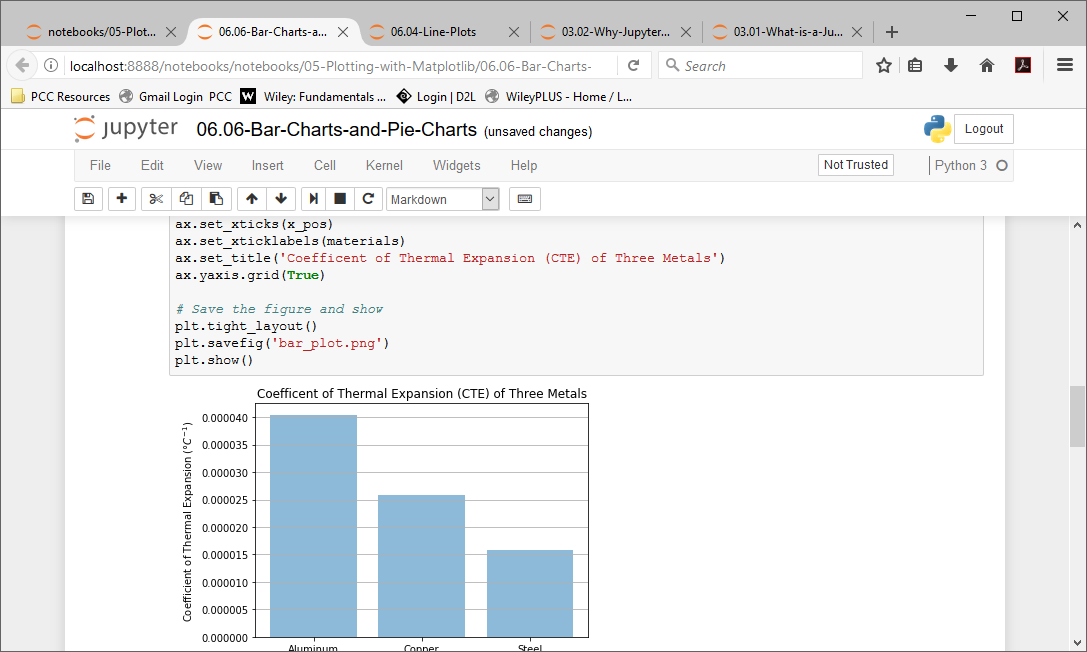
\includegraphics{images/jupyter_notebook_example.png}
\caption{Example Jupyter Notebook}
\end{figure}

In a way, Jupyter notebooks strike a balance between simple text
editors, which are fast to start and simple and easy to manipulate, and
IDE's which tend to start slower and be feature-rich and complex. Simple
text editors typically can only edit code, and cannot run the code. A
full IDE can edit code, run the code, debug code, provide syntax
highlighting and context help.
    




    
        In the context of problem-solving, Jupyter notebooks can be quite handy.
Jupyter notebooks are quick to open and quick to produce output. Data
exploration, data cleaning, and plot building are accomplished in
Jupyter notebooks easier and quicker than in a text editor or an IDE.

In the context of sharing solutions to problems, Jupyter notebooks are
also useful. Markdown cells render text in different sizes, bold and
italic. Tables and images, plots and code can all be shown together in
the same Jupyter notebook. Notebooks can be exported to a variety of
formats including \textbf{\emph{.html}} and \textbf{\emph{.pdf}}.
    



    \begin{Verbatim}[commandchars=\\\{\}]
{\color{incolor}In [{\color{incolor} }]:} 
\end{Verbatim}


    
        \hypertarget{installing-juypter}{%
\section{Installing Juypter}\label{installing-juypter}}
    




    
        The simplest way to install \textbf{Jupyter notebooks} is to download
and install the Anaconda distribution of Python. The Anaconda
distribution of Python comes with Jupyter notebook included and no
further installation steps are necessary.

Below are additional methods to install Jupyter notebooks if you are not
using the Anaconda distribution of Python.
    




    
        \hypertarget{installing-jupyter-on-windows-using-the-anaconda-prompt}{%
\subsection{Installing Jupyter on Windows using the Anaconda
Prompt}\label{installing-jupyter-on-windows-using-the-anaconda-prompt}}

To install Jupyter on Windows, open the \textbf{Anaconda Prompt} and
type:

\begin{lstlisting}
> conda install jupyter
\end{lstlisting}

Type \passthrough{\lstinline!y!} for yes when prompted. Once Jupyter is
installed, type the command below into the \textbf{Anaconda Prompt} to
open the Jupyter notebook file browser and start using Jupyter
notebooks.

\begin{lstlisting}
> jupyter notebook
\end{lstlisting}
    




    
        \hypertarget{installing-jupyter-on-macos}{%
\subsection{Installing Jupyter on
MacOS}\label{installing-jupyter-on-macos}}

To install Jupyter on MacOS, open the MacOS terminal and type:

\begin{lstlisting}
$ conda install jupyter
\end{lstlisting}

Type \passthrough{\lstinline!y!} for yes when prompted.

If \textbf{conda} is not installed, the Anaconda distribution of Python
can be installed, which will install \textbf{conda} for use in the MacOS
terminal.

Problems can crop up on MacOS when using the MacOS provided system
version of Python. Python packages may not install on the system version
of Python properly. Moreover, packages which do install on the system
version of Python may not run correctly. It is therefore recommended
that MacOS users install the \textbf{Anaconda} distribution of Python or
use \textbf{homebrew} to install a separate non-system version of
Python.

To install a non-system version of Python with \textbf{homebrew}, key
the following into the MacOS terminal:

\begin{lstlisting}
$ /usr/bin/ruby -e "$(curl -fsSL https://raw.githubusercontent.com/Homebrew/install/master/install)"
$ brew install Python
\end{lstlisting}

After \textbf{homebrew} installs a non-system version of Python,
\textbf{pip} can be used to install Jupyter.

\begin{lstlisting}
$ pip install jupyter
\end{lstlisting}
    




    
        \hypertarget{installing-jupyter-on-linux}{%
\subsection{Installing Jupyter on
Linux}\label{installing-jupyter-on-linux}}

To install Jupyter on Linux, open a terminal and type:

\begin{lstlisting}
$ conda install jupyter
\end{lstlisting}

Type \passthrough{\lstinline!y!} for yes when prompted.

Alternatively, if the Anaconda distribution of Python is not installed,
one can use \textbf{pip}.

\begin{lstlisting}
$ pip3 install jupyter
\end{lstlisting}
    



    \begin{Verbatim}[commandchars=\\\{\}]
{\color{incolor}In [{\color{incolor} }]:} 
\end{Verbatim}


    
        \hypertarget{opening-a-jupyter-notebook}{%
\section{Opening a Jupyter Notebook}\label{opening-a-jupyter-notebook}}
    




    
        In this section, you will learn how to open a Jupyter notebook on
Windows and MacOS.

One way problem solvers can write and execute Python code is in a
Jupyter notebook. Jupyter notebooks contain Python code, the output that
code produces and markdown cells usually used to explain what the code
means.

On Windows, a Jupyter notebook can be started from the \textbf{Anaconda
Prompt}, the Windows start menu and \textbf{Anaconda Navigator}.

\hypertarget{ways-to-open-a-jupyter-notebook}{%
\subsubsection{\texorpdfstring{3 ways to open a \textbf{Jupyter
notebook}:}{3 ways to open a Jupyter notebook:}}\label{ways-to-open-a-jupyter-notebook}}

\begin{itemize}
\item
  Windows Start Menu
\item
  \textbf{Anaconda Prompt}
\item
  Anaconda Navigator
\end{itemize}
    




    
        \hypertarget{open-a-jupyter-notebook-with-the-windows-start-menu}{%
\subsection{Open a Jupyter notebook with the Windows Start
Menu}\label{open-a-jupyter-notebook-with-the-windows-start-menu}}
    




    
        One simple way to open a Jupyter notebook is to use the Windows Start
Menu. Note that the Anaconda distribution of Python must be installed to
use the Windows Start Menu to open a Jupyter notebook. Download
\textbf{Anaconda} at the following link:
\href{https://www.anaconda.com/download/}{Anaconda.com/downloads}

Open the Windows start menu and select \textbf{{[}Anaconda3(64 bit){]}}
--\textgreater{} \textbf{{[}Jupyter Notebook{]}}

\begin{figure}
\centering
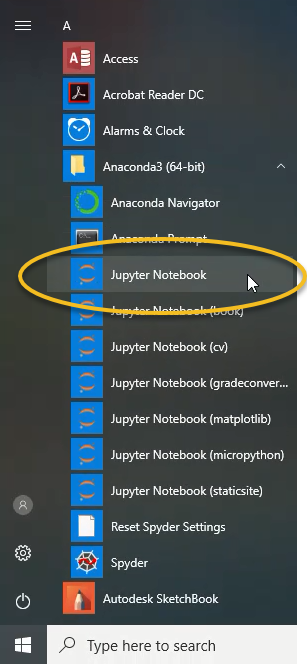
\includegraphics{images/windows_start_jupyter_notebook.png}
\caption{Windows 10 Start Menu showing the Jupyter Notebook application}
\end{figure}

This action opens the \textbf{Jupyter file browser} in a web browser
tab.

In the upper right select \textbf{{[}New{]}} --\textgreater{}
\textbf{{[}Python 3{]}}

\begin{figure}
\centering
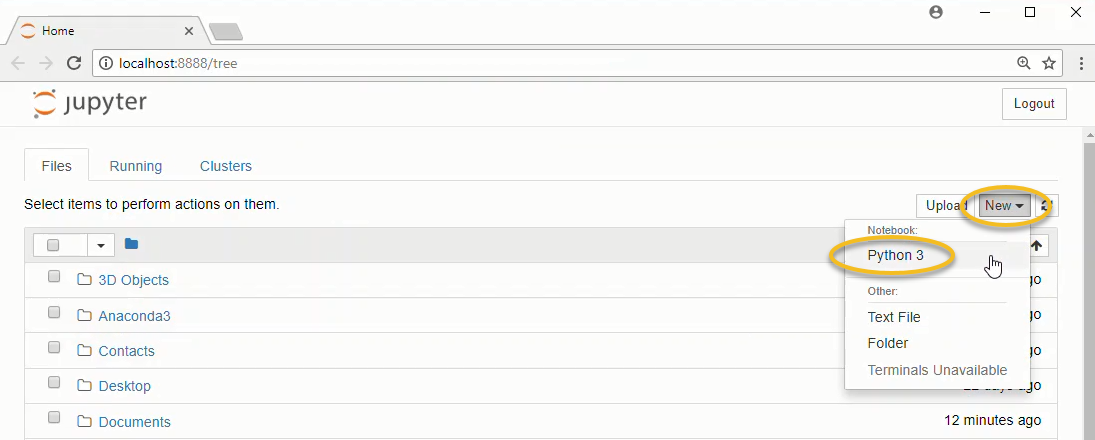
\includegraphics{images/new_notebook_from_browser.png}
\caption{Jupyter Notebook file browser}
\end{figure}

A new \textbf{notebook} will open as a new tab in your web browser.

\begin{figure}
\centering
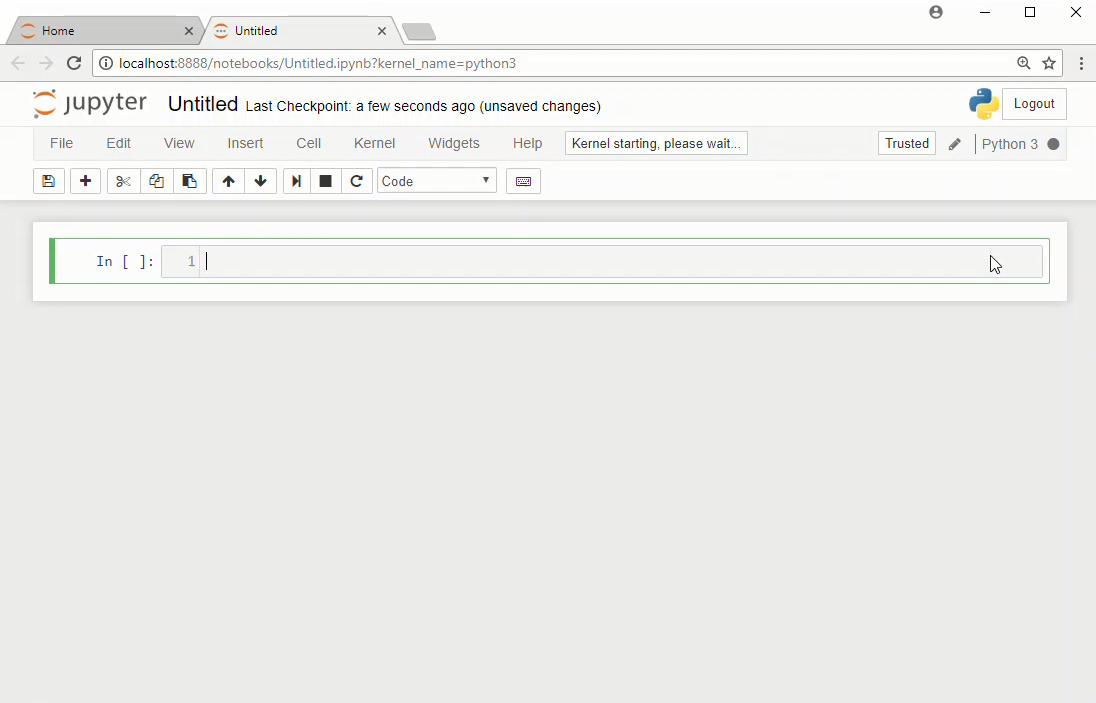
\includegraphics{images/new_notebook.png}
\caption{a newly opened Jupyter Nobebook}
\end{figure}

Try typing this in the first cell in the notebook to the right of the
\passthrough{\lstinline!In [ ]:!} prompt:

\begin{lstlisting}[language=Python]
import this
\end{lstlisting}

Then click the run button in the middle of the menu at the top of the
notebook.

\begin{figure}
\centering
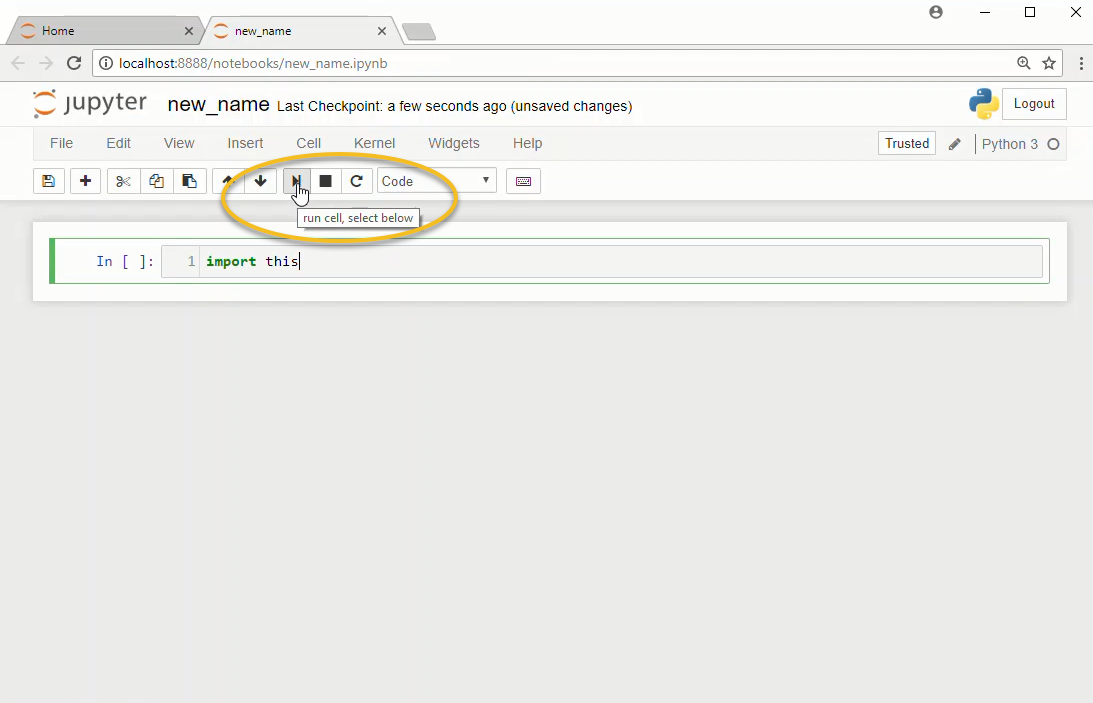
\includegraphics{images/run_import_this.png}
\caption{Jupyter Notebook running ``import this''}
\end{figure}
    




    
        \hypertarget{open-a-jupyter-notebook-with-the-anaconda-prompt}{%
\subsection{Open a Jupyter Notebook with the Anaconda
Prompt}\label{open-a-jupyter-notebook-with-the-anaconda-prompt}}
    




    
        Another method to open a Jupyter notebook is to use the \textbf{Anaconda
Prompt}.

Go to the Windows start menu and select \textbf{{[}Anaconda Prompt{]}}
under \textbf{{[}Anaconda3{]}}.

\begin{figure}
\centering
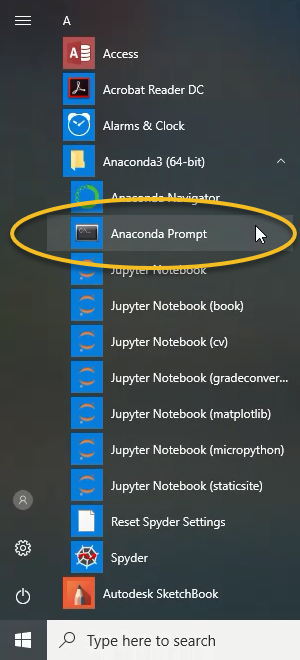
\includegraphics{images/anaconda_start_menu.png}
\caption{Windows 10 Start Menu showing the Anaconda Prompt application}
\end{figure}

If you don't see the \textbf{Anaconda Prompt} in the Windows Start Menu,
then you need to install the Anaconda distribution of Python. Download
\textbf{Anaconda} at the following link:
\href{https://www.anaconda.com/download/}{Anaconda.com/downloads}

The \textbf{Anaconda Prompt} window should look something like the image
below.

\begin{figure}
\centering
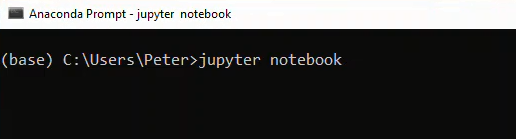
\includegraphics{images/jupyter_notebook_anaconda_prompt.png}
\caption{Anaconda Prompt}
\end{figure}

At the \textbf{Anaconda Prompt} type:

\begin{lstlisting}
> jupyter notebook
\end{lstlisting}

This command starts the \textbf{Jupyter notebook} server. The output in
the \textbf{Anaconda Prompt} will look something like the output shown
below:

\begin{lstlisting}

Copy/paste this URL into your browser when you connect for the first time,

    to login with a token:

        http://localhost:8888/?token=6bdef677d3503fbb23e1b4fa0c802e ...

[I 16:14:12.661 NotebookApp] Accepting one-time-token-authenticated ...
\end{lstlisting}

A web browser should open, and you should be able to see the
\textbf{Jupyter file browser}. If a web browser doesn't open
automatically, you can copy the web address from the \textbf{Anaconda
Prompt} and paste it into a web browser's address bar.

\begin{figure}
\centering
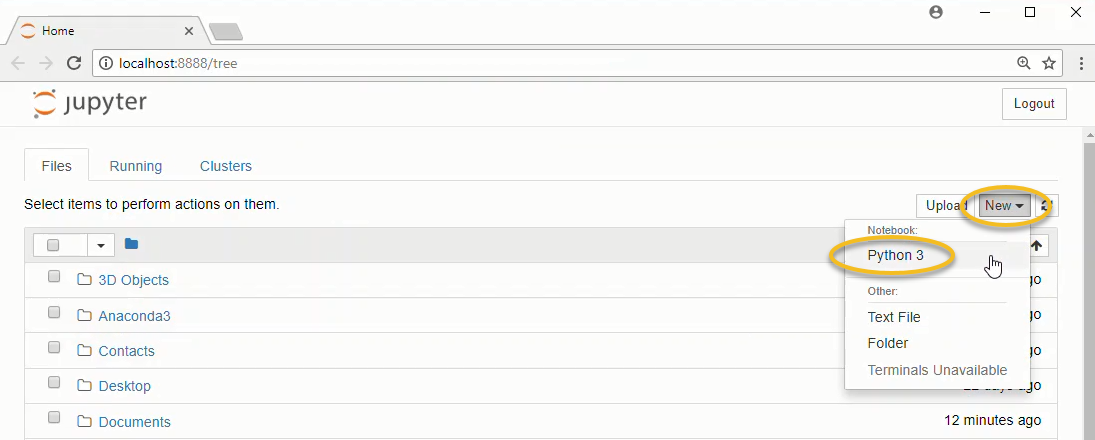
\includegraphics{images/new_notebook_from_browser.png}
\caption{Jupyter Notebook file browser- create new notebook}
\end{figure}

In the upper right select \textbf{{[}New{]}} --\textgreater{}
\textbf{{[}Python 3{]}}

You will see a new tab open in your web browser. This web browser page
is a \textbf{Jupyter notebook}.

\begin{figure}
\centering
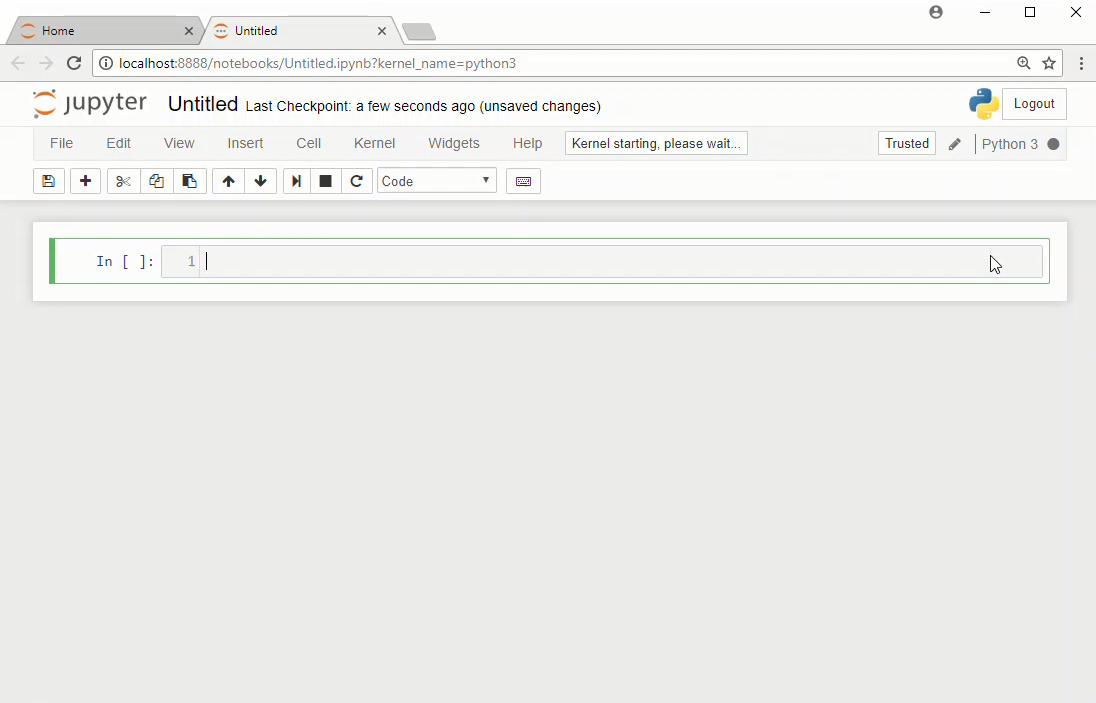
\includegraphics{images/new_notebook.png}
\caption{Newly opened Jupyter Notebook}
\end{figure}
    




    
        \hypertarget{open-a-jupyter-notebook-with-anaconda-navigator}{%
\subsection{Open a Jupyter Notebook with Anaconda
Navigator}\label{open-a-jupyter-notebook-with-anaconda-navigator}}
    




    
        One additional way to open a Jupyter notebook is to use \textbf{Anaconda
Navigator}. Anaconda Navigator comes with the Anaconda distribution of
Python. Open \textbf{Anaconda Navigator} using the Windows start menu
and select \textbf{{[}Anaconda3(64-bit){]}} --\textgreater{}
\textbf{{[}Anaconda Navigator{]}}.

\begin{figure}
\centering
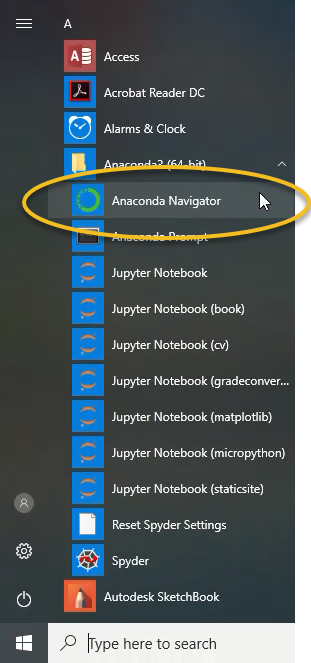
\includegraphics{images/windows_start_anaconda_navigator.png}
\caption{Windows 10 Start Menu showing the Anaconda Navigator
application}
\end{figure}

An \textbf{Anaconda Navigator} window will open. In the middle of the
page, in the \textbf{Jupyter notebook} tile, click \textbf{{[}Launch{]}}

\begin{figure}
\centering
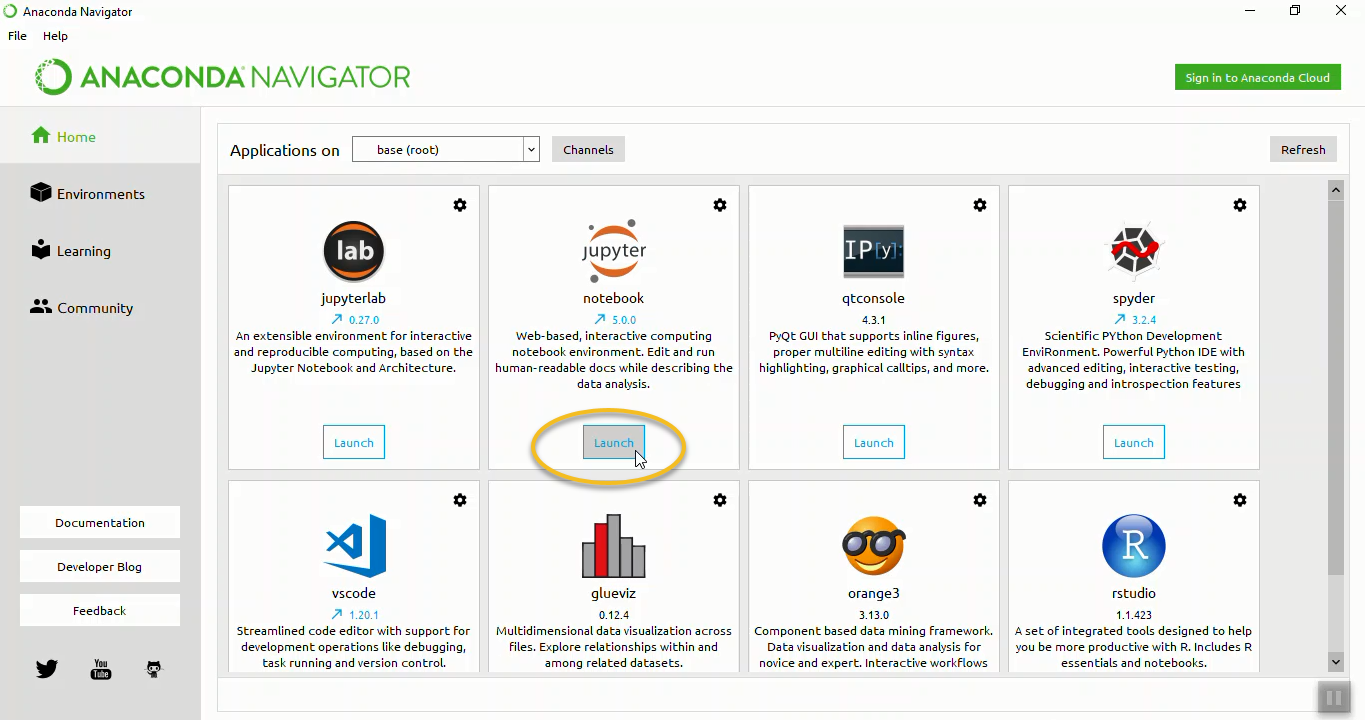
\includegraphics{images/anaconda_navigator_jupyter_notebook_launch.png}
\caption{Anaconda Navigator- launch new Jupyter Notebook}
\end{figure}

A \textbf{Jupyter file browser} will open in a web browser tab.

In the upper right select \textbf{{[}New{]}} --\textgreater{}
\textbf{{[}Python 3{]}}

\begin{figure}
\centering
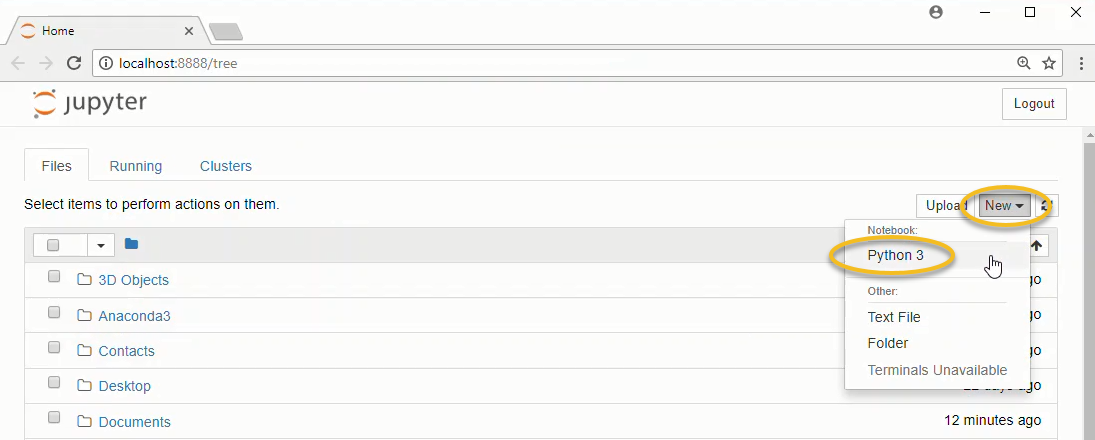
\includegraphics{images/new_notebook_from_browser.png}
\caption{Jupyter Notebook file browser - create new Notebook}
\end{figure}

A new \textbf{notebook} will open as a new tab in your web browser.

\begin{figure}
\centering
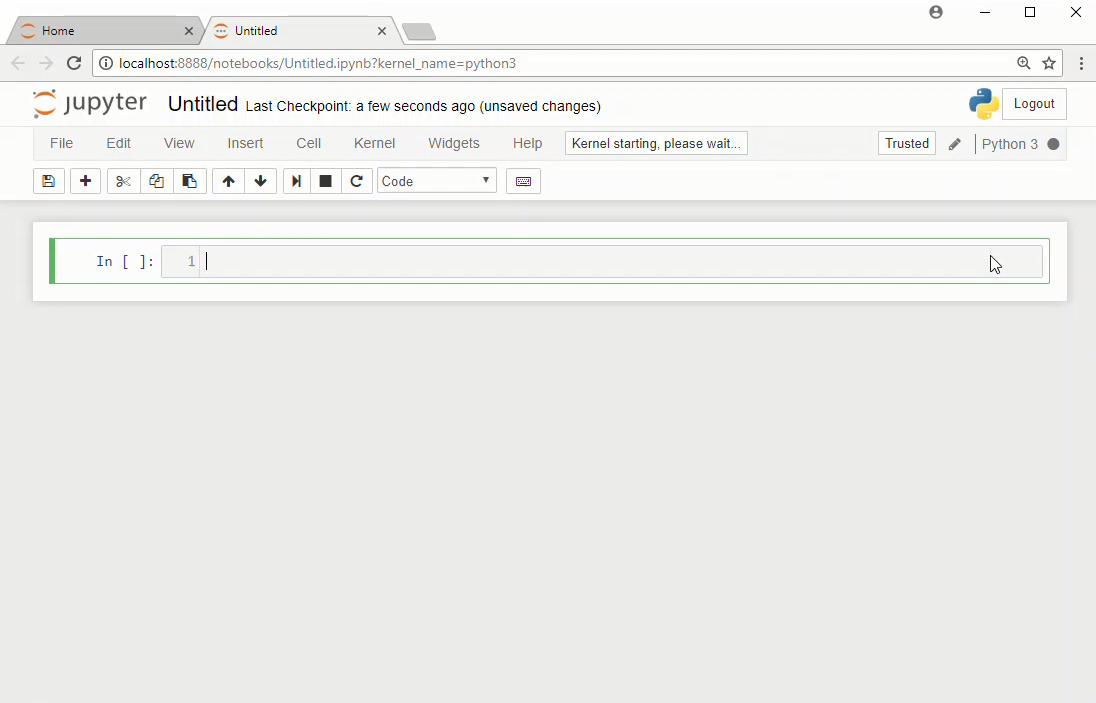
\includegraphics{images/new_notebook.png}
\caption{Newly opened Jupyter Notebook}
\end{figure}
    



    \begin{Verbatim}[commandchars=\\\{\}]
{\color{incolor}In [{\color{incolor} }]:} 
\end{Verbatim}


    
        \hypertarget{the-jupyter-notebook-interface}{%
\section{The Jupyter Notebook
Interface}\label{the-jupyter-notebook-interface}}
    




    
        When a new Jupyter notebook opens, you will see the Jupyter notebook
interface. Across the top of the notebook you see the Jupyter icon and
the Notebook name. You can click on the notebook name field and change
the name of the notebook. Note that the file extension
\passthrough{\lstinline!.ipynb!} is not printed in the file name field,
but if you look in the Home tab, you will see that the notebook is saved
with the \passthrough{\lstinline!.ipynb!} extension.
    




    
        \hypertarget{menus-and-buttons}{%
\subsection{Menus and Buttons}\label{menus-and-buttons}}

A Jupyter notebook is comprised of a bunch of \emph{cells} which are
arrayed one after another in boxes below the menu items and buttons.
There are three main types of cells: code cells, output cells, and
markdown cells.
    




    
        \hypertarget{code-cells}{%
\subsection{Code Cells}\label{code-cells}}

In code cells, you can write Python code, then execute the Python code
and see the resulting output. An example of a code cell is shown below.

\begin{figure}
\centering
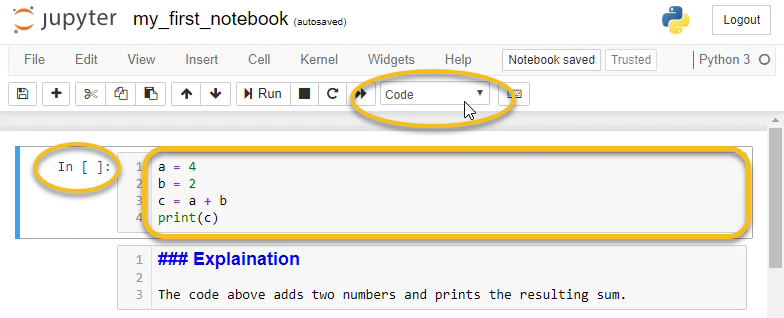
\includegraphics{images/code_cell.png}
\caption{Jupyter Notebook Code Cell}
\end{figure}

You can tell you are typing in a code cell because
\passthrough{\lstinline!In [ ]:!} is shown to the left of the cell and
the cell-type drop-down menu shows \textbf{Code}.

To run the Python code in a code cell push the {[}Run{]} button or type
{[}Shift{]}+{[}Enter{]}. Hitting {[}Enter{]} when the cursor is inside a
code cell brings the cursor down to a new line.

\begin{figure}
\centering
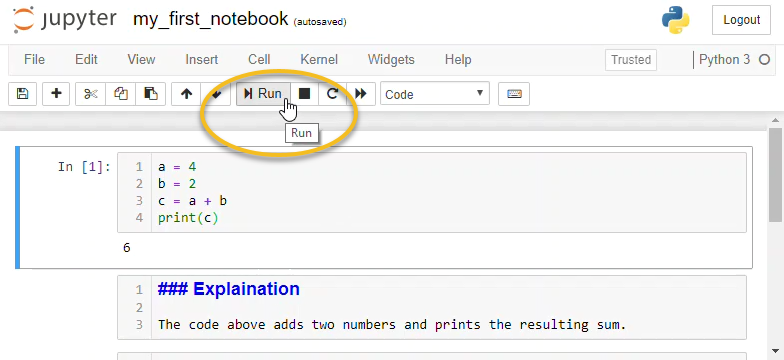
\includegraphics{images/run_cell.png}
\caption{Jupyter Notebook Run Cell}
\end{figure}
    




    
        \hypertarget{output-cells}{%
\subsection{Output Cells}\label{output-cells}}

After a code cell is run, an output cell can be produced below the code
cell. The output cell contains the output from the code cell above it.
Not all code produces output, so not all code cells produce output
cells. The results in output cells can't be edited. If a code cell
produces plots, charts or images, these outputs are shown in output
cells.

\begin{figure}
\centering
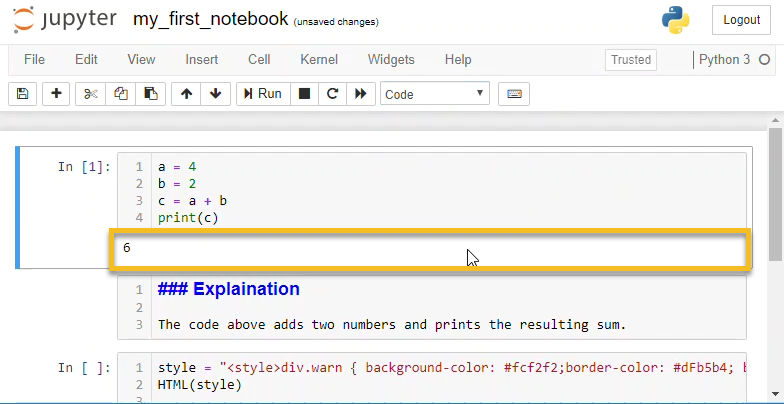
\includegraphics{images/output_cell.png}
\caption{Jupyter Notebook Output Cell}
\end{figure}

You can clear all the output cells and re-run code cells by selecting
\textbf{{[}Kernal{]}} --\textgreater{} \textbf{{[}Restart Kernal and
Clear Output{]}}.

\begin{figure}
\centering
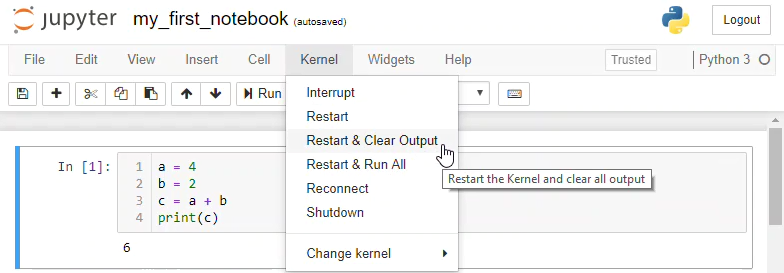
\includegraphics{images/kernel_restart_and_clear_output.png}
\caption{Jupyter Notebook Clear All Outputs}
\end{figure}
    




    
        \hypertarget{markdown-cells}{%
\subsection{Markdown Cells}\label{markdown-cells}}

Markdown cells don't contain Python code. Markdown cells contain text
written in Markdown format. Text in markdown cells can be formatted to
show \textbf{bold} or \emph{italic} text. Tables, images, and lists can
also be included in markdown cells.

\begin{figure}
\centering
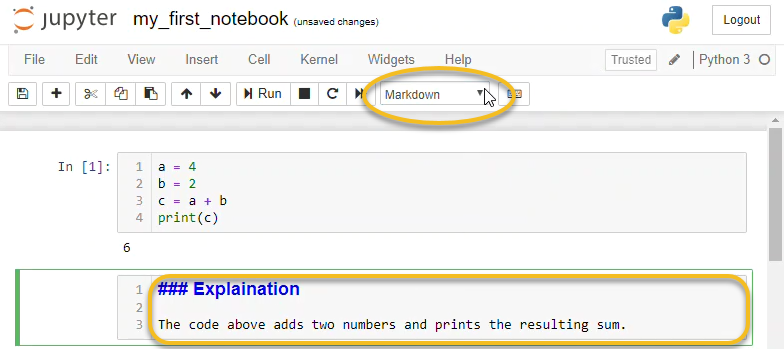
\includegraphics{images/markdown_cell.png}
\caption{Jupyter Notebook Markdown Cell}
\end{figure}

Markdown cells are used for documentation and explaining your code. The
text in a markdown cell is not executed. Markdown cells can be formatted
with a few special characters.

Markdown cells are run like code cells. The difference is that when
markdown cells are run, the text is formatted (when code cells run, code
is executed). Markdown cells are run by clicking the {[}Run{]} button or
by pressing \passthrough{\lstinline![Shift]!} +
\passthrough{\lstinline![Enter]!}

Text in markdown cells can be formatted using \emph{markdown syntax}. An
example of markdown syntax is putting an underscore before and after a
word to cause the word to be formatted in \emph{italics}.

\hypertarget{headings}{%
\subsubsection{Headings}\label{headings}}

Headings are created in markdown cells using the hash symbol
\passthrough{\lstinline!#!}. One \passthrough{\lstinline!#!} is the
largest heading. Four hashes \passthrough{\lstinline!####!} is the
smallest heading.

\begin{lstlisting}
# H1 Heading
\end{lstlisting}

\begin{lstlisting}
## H2 Heading
\end{lstlisting}

\begin{lstlisting}
### H3 Heading
\end{lstlisting}

\begin{lstlisting}
#### H4 Heading
\end{lstlisting}

\hypertarget{code-blocks}{%
\subsubsection{Code Blocks}\label{code-blocks}}

Code blocks can be inserted in Jupyter notebook markdown cells. For
inline code blocks use the ` left quote character, the character to the
left of the number \passthrough{\lstinline![1]``` and above ```[Tab]!}
on most keyboards.

This is inline code: ` ` ` Inline code block ` ` ` within a paragraph

For a separated code block use three ` left quote characters on one
line, followed by the code block on separate lines. Terminate the
separate code block with a line of three ` left quote characters.

```

Separated code block

```

\hypertarget{bold-and-italics}{%
\subsubsection{Bold and italics}\label{bold-and-italics}}

\textbf{Bold} and \emph{italic font} is displayed by surrounding text
with a double asterisk for \passthrough{\lstinline!**bold**!} and a
single underscore for \passthrough{\lstinline!\_italics\_!}

\passthrough{\lstinline!**bold**!} produces \textbf{bold}

\passthrough{\lstinline!\_italics\_!} produces \emph{italics}

\passthrough{\lstinline!**\_bold and italic\_**!} produces
\textbf{\emph{bold and italic}}

\hypertarget{tables}{%
\subsubsection{Tables}\label{tables}}

Tables are displayed using the pipe \passthrough{\lstinline!|!}
character, which is {[}Shift{]}+{[}\textbackslash{}{]} on most
keyboards. Columns are separated by pipes \passthrough{\lstinline!|!}
and rows are separated by lines. After the header row, a row of pipes
and dashes \passthrough{\lstinline!---!} are needed to define the table.

\begin{lstlisting}
| header1 | header 2 | header 3 |
| --- | --- | --- |
| col 1 | col 2 | col 3 |
| col 1 | col 2 | col 3 |
\end{lstlisting}

produces:

\begin{longtable}[]{@{}lll@{}}
\toprule
header1 & header 2 & header 3\tabularnewline
\midrule
\endhead
col 1 & col 2 & col 3\tabularnewline
col 1 & col 2 & col 3\tabularnewline
\bottomrule
\end{longtable}

\hypertarget{bullet-points-and-lists}{%
\subsubsection{Bullet Points and Lists}\label{bullet-points-and-lists}}

Bullet points are produced using the asterisk character
\passthrough{\lstinline!*!}

\begin{lstlisting}
 * item 1
 * item 2
 * item 3
\end{lstlisting}

produces

\begin{itemize}
\tightlist
\item
  item 1
\item
  item 2
\end{itemize}

Numbered lists are produced using sequential numbers followed by a dot.
Indent sub-items with two spaces.

\begin{lstlisting}
1. First item
2. Second item
3. Third item
  1. sub item
  2. sub item
    1. sub-sub item
    2. sub-sub item
\end{lstlisting}

produces

\begin{enumerate}
\def\labelenumi{\arabic{enumi}.}
\tightlist
\item
  First item
\item
  Second item
\item
  Third item
\item
  sub item
\item
  sub item 1. sub-sub item 2. sub-sub item
\end{enumerate}

\hypertarget{horizontal-rule}{%
\subsubsection{Horizontal Rule}\label{horizontal-rule}}

A horizontal rule is specified with three asterisks
\passthrough{\lstinline!***!} on a single line.

\begin{lstlisting}
***
\end{lstlisting}

produces

\begin{center}\rule{0.5\linewidth}{\linethickness}\end{center}

\hypertarget{links}{%
\subsubsection{Links}\label{links}}

Hyperlinks are specified using a set of square brackets
\passthrough{\lstinline![ ]!} followed by a pair of parenthesis
\passthrough{\lstinline!( )!} The text inside the square brackets will
be the link, the link address goes in the parenthesis.

\begin{lstlisting}
[Problem Solving with Python Book Link](https://problemsolvingwithpython.com/)
\end{lstlisting}

produces

\href{https://problemsolvingwithpython.com/}{Problem Solving with Python
Book Link}

\hypertarget{images}{%
\subsubsection{Images}\label{images}}

Images are embedded in Jupyter Notebook markdown using the exclamation
point and square brackets \passthrough{\lstinline"![ ]"}, followed by
the image file path in parenthesis \passthrough{\lstinline!( )!}. If the
image can not be displayed, the text in square brackets will be shown.
The image can be in the same directory as the notebook, or a relative
path can be specified. In this case, the image
\passthrough{\lstinline!engineering.png!} is stored in the
\passthrough{\lstinline!images!} directory, which is a subdirectory of
the directory the notebook is saved in.

\begin{lstlisting}
![Engineering Image](images/engineering.png)
\end{lstlisting}

produces

\begin{figure}
\centering

\includegraphics{images/engineering.png}
\caption{Image displayed in a Jupyter notebook}
\end{figure}

\hypertarget{latex-math}{%
\subsubsection{LaTeX Math}\label{latex-math}}

LaTeX Math equations and symbols are rendered by markdown cells. A more
extensive list of LaTeX commands can be found in the appendix.

\begin{lstlisting}
$$ \int_{a}^{b} \frac{1}{x^2} dx $$
\end{lstlisting}

produces

\[ \int_{a}^{b} \frac{1}{x^2} dx \]

\hypertarget{html}{%
\subsubsection{html}\label{html}}

Because Jupyter notebooks are rendered by web browsers, just about any
HTML tag can be included in the markdown portion of a notebook. An
example of an HTML tag is the \passthrough{\lstinline!<sup>!}
\passthrough{\lstinline!</sup>!} tags that surround superscript text.

\begin{lstlisting}
x<sup>2</sup>
\end{lstlisting}

produces

x2

Text can be colored using html \passthrough{\lstinline!<font>!}
\passthrough{\lstinline!</font>!} tags

\begin{lstlisting}
<font color=red>Red Text</font>
\end{lstlisting}

produces

Red Text

\hypertarget{warning-boxes}{%
\subsubsection{warning boxes}\label{warning-boxes}}

bootstrap style warning boxes can be included in Jupyter notebook
markdown using \passthrough{\lstinline!<div>!} tags

\begin{lstlisting}
<div class="alert alert-danger" role="alert">
  <strong>Warning!</strong> Python lists start at 0
</div>
\end{lstlisting}

produces

Warning! Python lists start at 0
    




    
        \hypertarget{creating-a-new-cell}{%
\subsection{Creating a new cell}\label{creating-a-new-cell}}

You can create a new cell in a Jupyter Notebook by clicking the {[}+{]}
button in the upper menu. Clicking the {[}+{]} button produces a new
code cell below the currently active cell.

\begin{figure}
\centering
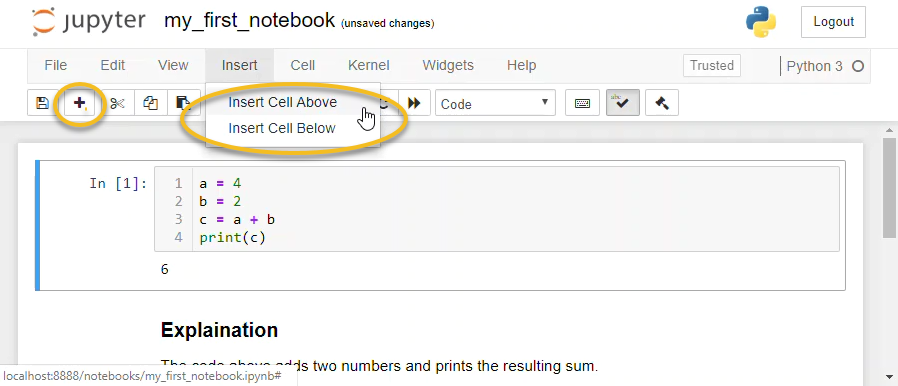
\includegraphics{images/insert_cell_above.png}
\caption{Jupyter Notebook New Cell Button}
\end{figure}

You can also create a new cell using \textbf{Insert} --\textgreater{}
\textbf{Insert Cell Above} or \textbf{Insert Cell Below}. You can choose
to insert a cell above or below the currently active cell.
    




    
        \hypertarget{changing-the-cell-type}{%
\subsection{Changing the cell type}\label{changing-the-cell-type}}

The type of cell: code cell or markdown cell, is changed by clicking on
a cell and selecting the cell type from the drop-down menu. Typing
\passthrough{\lstinline![Esc]!} + \passthrough{\lstinline![m]!} changes
the cell type to a markdown cell. Typing \passthrough{\lstinline![Esc]!}
+ \passthrough{\lstinline![y]!} changes the cell type to a code cell.

\begin{figure}
\centering
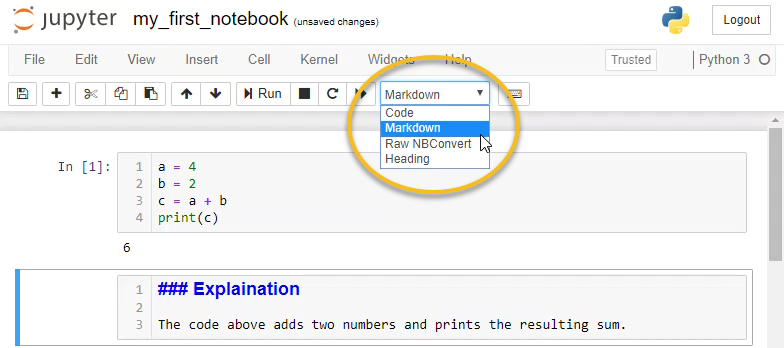
\includegraphics{images/change_cell_type.png}
\caption{Jupyter Notebook Change Cell Type}
\end{figure}
    




    
        \hypertarget{saving-a-jupyter-notebook}{%
\subsection{Saving a Jupyter Notebook}\label{saving-a-jupyter-notebook}}

Jupyter notebooks can be saved using the save icon in the upper menu or
by pressing {[}Ctrl{]} + {[}s{]}.

\begin{figure}
\centering
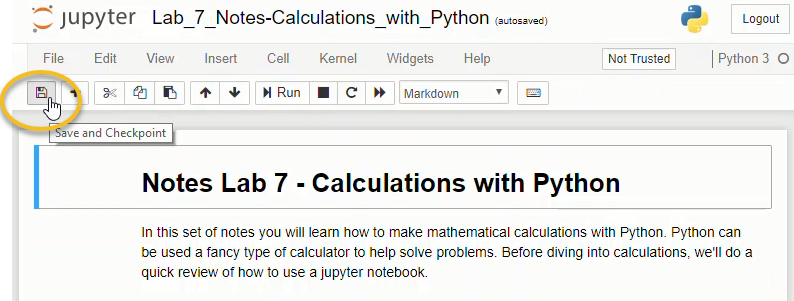
\includegraphics{images/save_notebook.png}
\caption{Jupyter Notebook Save}
\end{figure}

Jupyter notebooks can also be saved as a copy, similar to the Save As
command common in many programs. To save a copy of a Jupyter notebook
use \textbf{File} --\textgreater{} \textbf{Make a Copy\ldots{}}

\begin{figure}
\centering
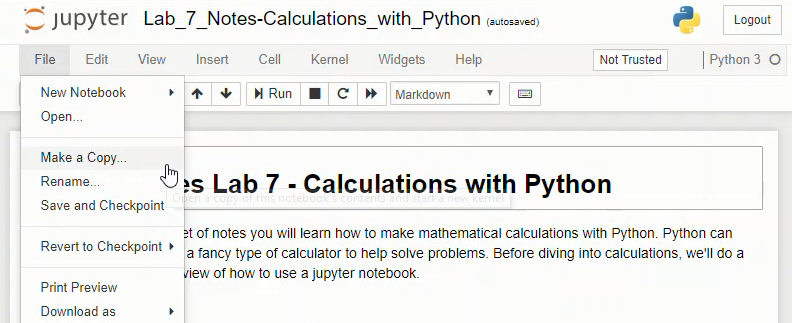
\includegraphics{images/file_make_a_copy.png}
\caption{Jupyter Notebook save a copy}
\end{figure}
    




    
        \hypertarget{renaming-a-jupyter-notebook}{%
\subsection{Renaming a Jupyter
Notebook}\label{renaming-a-jupyter-notebook}}

Jupyter notebooks are renamed by clicking on the notebook name above the
upper menu and typing a new name into the dialog box.

\begin{figure}
\centering
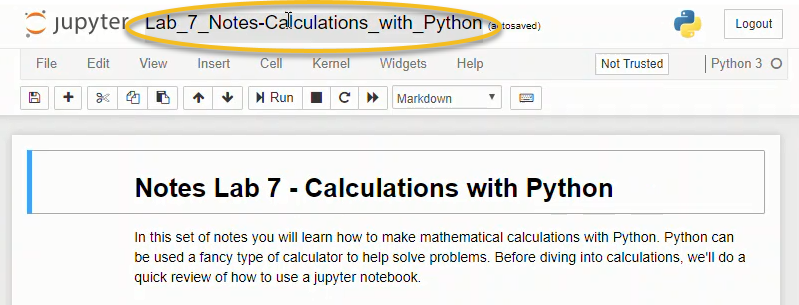
\includegraphics{images/rename_notebook.png}
\caption{Jupyter Notebook rename notebook}
\end{figure}

\begin{figure}
\centering
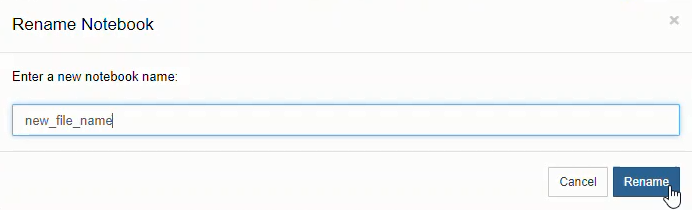
\includegraphics{images/rename_dialog.png}
\caption{Jupyter Notebook rename dialog box}
\end{figure}
    




    
        \hypertarget{downloading-a-jupyter-notebook}{%
\subsection{Downloading a Jupyter
Notebook}\label{downloading-a-jupyter-notebook}}

Jupyter notebooks can be downloaded and saved using \textbf{File
--\textgreater{} Download As --\textgreater{} Notebook (.ipynb)}.
Selecting this menu option will download the notebook as a
\passthrough{\lstinline!.ipynb!} file.

\begin{figure}
\centering
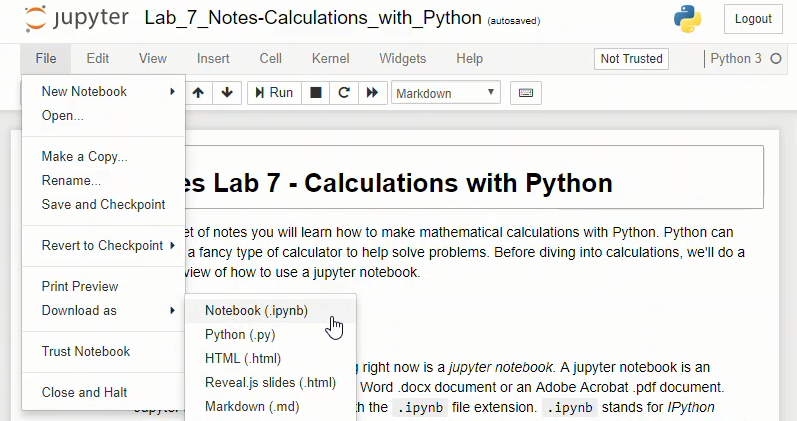
\includegraphics{images/file_download_as_notebook.png}
\caption{Jupyter Notebook downloaded as .ipynb file}
\end{figure}

Note that when a \passthrough{\lstinline!.ipynb!} file is viewed in a
text editor like notepad, the notebook is unformatted and looks like a
confusing jumble of text. The notebook needs to be opened in a Jupyter
notebook file browser in order for the code in the notebook to run and
the markdown text to render.

\begin{figure}
\centering
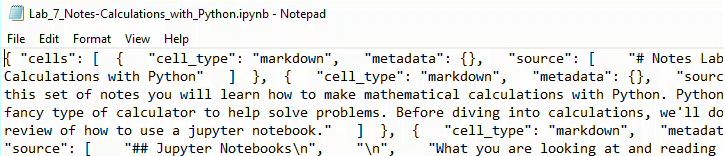
\includegraphics{images/notebook_json.png}
\caption{Jupyter Notebook JSON in notepad}
\end{figure}
    




    
        \hypertarget{saving-jupyter-notebooks-in-other-formats}{%
\subsection{Saving Jupyter Notebooks in Other
Formats}\label{saving-jupyter-notebooks-in-other-formats}}

Jupyter notebooks can be saved in other formats besides the native
\passthrough{\lstinline!.ipynb!} format. These formats can be accessed
using the \textbf{{[}File{]} --\textgreater{} {[}Download As{]}} menu.

\begin{figure}
\centering
\includegraphics{images/jupyter_notebook_export_options.png}
\caption{Jupyter Notebook Export Optinos}
\end{figure}

The available file download types are:

\begin{itemize}
\tightlist
\item
  Notebook (.ipynb) - The native jupyter notebook format
\item
  Python (.py) - The native Python code file type.
\item
  HTML (.html) - A web page
\item
  Markdown (.md) - Markdown format
\item
  reST (.rst) - Restructured text format
\item
  LaTeX (.tex) - LaTeX Article format
\item
  PDF via LaTeX - a pdf exported from LeTeX, requires a converter
\end{itemize}

When a Notebook is saved as a \passthrough{\lstinline!.py!} file, all
text in markdown cells is converted to comments, and any code cells stay
intact as Python code.

\begin{figure}
\centering
\includegraphics{images/jupyter_notebook_markdown_cells_as_comments.png}
\caption{Markdown Cells as Comments}
\end{figure}
    



    \begin{Verbatim}[commandchars=\\\{\}]
{\color{incolor}In [{\color{incolor} }]:} 
\end{Verbatim}


    
        \hypertarget{magic-cells}{%
\section{Magic Cells}\label{magic-cells}}
    




    
        Jupyter notebook code cells can contain special commands which are not
valid Python code but affect the behavior of the notebook.
    




    
        \hypertarget{matplotlib-inline}{%
\subsection{\%matplotlib inline}\label{matplotlib-inline}}
    




    
        \hypertarget{matplotlib-inline}{%
\subsection{\%matplotlib inline}\label{matplotlib-inline}}

One of the most popular magic commands is:

\begin{lstlisting}
%matplotlib inline
\end{lstlisting}

Entering the \passthrough{\lstinline!\%matplotlib inline!} command at
the top of a Jupyter notebook renders Matplotlib plots in cells of the
notebook. Without \passthrough{\lstinline!\%matplotlib inline!}, plots
may jump out as external windows. A typical start to a Jupyter notebook
using \textbf{Matplotlib} might start as:

\begin{lstlisting}[language=Python]
import numpy as np
import pandas as pd
import matplotlib.pyplot as plt
%matplotlib inline
\end{lstlisting}
    




    
        \hypertarget{load}{%
\subsection{\%load}\label{load}}

The \passthrough{\lstinline!\%load!} command loads a Python module,
webpage or file into a Jupyter notebook. If there is a file called
\textbf{\emph{hello.py}} in the same directory as the notebook with some
Python code written in it, we can load that same code into a Jupyter
notebook code cell with the \passthrough{\lstinline!\%load!} command.

Within a Jupyter notebook code cell type the command:

\begin{lstlisting}[language=Python]
%load hello.py
\end{lstlisting}

The result is the code from the file \textbf{\emph{hello.py}} is copied
into the current notebook.
    



    \begin{Verbatim}[commandchars=\\\{\}]
{\color{incolor}In [{\color{incolor}1}]:} \PY{c+c1}{\PYZsh{} \PYZpc{}load hello.py}
        \PY{c+c1}{\PYZsh{} hello.py}
        
        \PY{n+nb}{print}\PY{p}{(}\PY{l+s+s1}{\PYZsq{}}\PY{l+s+s1}{This code was run from a seperate Python file}\PY{l+s+s1}{\PYZsq{}}\PY{p}{)}
        \PY{n+nb}{print}\PY{p}{(}\PY{l+s+s1}{\PYZsq{}}\PY{l+s+s1}{Hello from the file hello.py}\PY{l+s+s1}{\PYZsq{}}\PY{p}{)}
\end{Verbatim}

    \begin{Verbatim}[commandchars=\\\{\}]
This code was run from a seperate Python file
Hello from the file hello.py

    \end{Verbatim}


    
        \hypertarget{run}{%
\subsection{\%run}\label{run}}
    




    
        If the \passthrough{\lstinline!\%run!} magic command followed by the
name of a valid Python file, the Python file runs as a script. Suppose
the file \passthrough{\lstinline!hello.py!} is created in the same
directory as the running Jupyter notebook. The directory structure will
look something like this:

\begin{lstlisting}
| folder
---| notebook.ipynb
---| hello.py
\end{lstlisting}

In the file \passthrough{\lstinline!hello.py!} is the code:

\begin{lstlisting}[language=Python]
# hello.py

print('This code was run from a separate Python file')
print('Hello from the file hello.py')
\end{lstlisting}

Within our Jupyter notebook, if we \passthrough{\lstinline!\%run!} this
file, we get the output of the \textbf{\emph{hello.py}} script in a
Jupyter notebook output cell.
    



    \begin{Verbatim}[commandchars=\\\{\}]
{\color{incolor}In [{\color{incolor}2}]:} \PY{o}{\PYZpc{}}\PY{k}{run} hello.py
\end{Verbatim}

    \begin{Verbatim}[commandchars=\\\{\}]
This code was run from a separate Python file
Hello from the file hello.py

    \end{Verbatim}


    
        \hypertarget{other-useful-magic-commands}{%
\subsection{Other useful magic
commands}\label{other-useful-magic-commands}}
    




    
        Below is a table of other useful Jupyter notebook magic commands

\begin{longtable}[]{@{}ll@{}}
\toprule
magic command & result\tabularnewline
\midrule
\endhead
\%pwd & print the current working directory\tabularnewline
\%cd & change the current working directory\tabularnewline
\%ls & list the contents of the current directory\tabularnewline
\%history & the history of the \passthrough{\lstinline!In [ ]:!}
commands\tabularnewline
\bottomrule
\end{longtable}

You can list all of the available magic commands by typing and running
\passthrough{\lstinline!\%lsmagic!} in a Jupyter notebook code cell:

\begin{lstlisting}[language=Python]
%lsmagic
\end{lstlisting}

The output shows all the available line magic commands that begin with
the percent sign \passthrough{\lstinline!\%!}.

\begin{lstlisting}
Available line magics:
%alias  %alias_magic  %autocall  %automagic  %autosave ...
%dhist  %dirs  %doctest_mode  %ed  %edit  %env  %gui ...
dir  %more  %mv  %notebook  %page  %pastebin  %pdb  %pdef ...
...

Available cell magics:
%%!  %%HTML  %%SVG  %%bash  %%capture  %%debug  %%file  %%html ...
%%python  %%python2  %%python3  %%ruby  %%script  %%sh  %%svg ...
\end{lstlisting}
    



    \begin{Verbatim}[commandchars=\\\{\}]
{\color{incolor}In [{\color{incolor} }]:} 
\end{Verbatim}


    
        \hypertarget{getting-help-in-a-jupyter-notebook}{%
\section{Getting Help in a Jupyter
Notebook}\label{getting-help-in-a-jupyter-notebook}}
    




    
        There are a couple of different ways to get help when using a Jupyter
notebook.
    




    
        \hypertarget{get-help-using-dir}{%
\subsection{\texorpdfstring{Get help using
\texttt{dir}}{Get help using dir}}\label{get-help-using-dir}}

Typing \passthrough{\lstinline!dir()!} and passing in a function,
method, variable or object shows the possible object, method and
function calls available to that object. For example, we can investigate
the different functions in the \textbf{glob} module, part of Python's
Standard Library, by importing \passthrough{\lstinline!glob!}, then
calling \passthrough{\lstinline!dir(glob)!}.
    



    \begin{Verbatim}[commandchars=\\\{\}]
{\color{incolor}In [{\color{incolor}1}]:} \PY{k+kn}{import} \PY{n+nn}{glob}
        \PY{n+nb}{dir}\PY{p}{(}\PY{n}{glob}\PY{p}{)}
\end{Verbatim}

\begin{Verbatim}[commandchars=\\\{\}]
{\color{outcolor}Out[{\color{outcolor}1}]:} ['\_\_all\_\_',
         '\_\_builtins\_\_',
         '\_\_cached\_\_',
         '\_\_doc\_\_',
         '\_\_file\_\_',
         '\_\_loader\_\_',
         '\_\_name\_\_',
         '\_\_package\_\_',
         '\_\_spec\_\_',
         '\_glob0',
         '\_glob1',
         '\_glob2',
         '\_iglob',
         '\_ishidden',
         '\_isrecursive',
         '\_iterdir',
         '\_rlistdir',
         'escape',
         'fnmatch',
         'glob',
         'glob0',
         'glob1',
         'has\_magic',
         'iglob',
         'magic\_check',
         'magic\_check\_bytes',
         'os',
         're']
\end{Verbatim}
            

    
        \hypertarget{get-help-using-tab}{%
\subsection{Get help using Tab}\label{get-help-using-tab}}

After typing the name of a variable, object or function following the
\passthrough{\lstinline!.!} character hit the \textbf{{[}Tab{]}} key.
Typing \textbf{{[}Tab{]}} brings up a list of available options. Scroll
through the list or type a letter to filter the list to certain starting
letters. Use {[}Enter{]} to select the option you want.

Tab completion can also be used during module import. Hit tab after
typing the module name to see which functions and classes are available
in that module.
    




    
        \begin{lstlisting}[language=Python]
from math import <tab>
\end{lstlisting}
    




    
        \hypertarget{get-help-using-the-help-function}{%
\subsection{\texorpdfstring{Get help using the \texttt{help()}
function}{Get help using the help() function}}\label{get-help-using-the-help-function}}

After importing a module, you can use the
\passthrough{\lstinline!help()!} function to see documentation about the
command if it is available.
    



    \begin{Verbatim}[commandchars=\\\{\}]
{\color{incolor}In [{\color{incolor}2}]:} \PY{k+kn}{import} \PY{n+nn}{math}
        \PY{n}{help}\PY{p}{(}\PY{n}{math}\PY{o}{.}\PY{n}{sin}\PY{p}{)}
\end{Verbatim}

    \begin{Verbatim}[commandchars=\\\{\}]
Help on built-in function sin in module math:

sin({\ldots})
    sin(x)
    
    Return the sine of x (measured in radians).


    \end{Verbatim}


    
        After importing a module, you can view help on the imported module by
typing the module name followed by a question mark
\passthrough{\lstinline!?!}
    



    \begin{Verbatim}[commandchars=\\\{\}]
{\color{incolor}In [{\color{incolor}3}]:} \PY{k+kn}{import} \PY{n+nn}{statistics}
        statistics.mean\PY{o}{?}
\end{Verbatim}


    
        \begin{lstlisting}
Signature: statistics.mean(data)
Docstring:
Return the sample arithmetic mean of data.

>>> mean([1, 2, 3, 4, 4])
2.8

>>> from fractions import Fraction as F
>>> mean([F(3, 7), F(1, 21), F(5, 3), F(1, 3)])
Fraction(13, 21)

>>> from decimal import Decimal as D
>>> mean([D("0.5"), D("0.75"), D("0.625"), D("0.375")])
Decimal('0.5625')

If ``data`` is empty, StatisticsError will be raised.
File:      ~/anaconda3/envs/book/lib/python3.6/statistics.py
Type:      function
\end{lstlisting}
    




    
        You can view the source code where a particular function is defined
using a double question mark \passthrough{\lstinline!??!}
    



    \begin{Verbatim}[commandchars=\\\{\}]
{\color{incolor}In [{\color{incolor}4}]:} \PY{k+kn}{import} \PY{n+nn}{statistics}
        statistics.mean\PY{o}{??}
\end{Verbatim}


    
        \begin{lstlisting}
Signature: statistics.mean(data)
Source:   
def mean(data):
    """Return the sample arithmetic mean of data.

    >>> mean([1, 2, 3, 4, 4])
    2.8

    >>> from fractions import Fraction as F
    >>> mean([F(3, 7), F(1, 21), F(5, 3), F(1, 3)])
    Fraction(13, 21)

    >>> from decimal import Decimal as D
    >>> mean([D("0.5"), D("0.75"), D("0.625"), D("0.375")])
    Decimal('0.5625')

    If ``data`` is empty, StatisticsError will be raised.
    """
    if iter(data) is data:
        data = list(data)
\end{lstlisting}
    




    
        \hypertarget{help-online}{%
\subsection{Help online}\label{help-online}}

Help is also available online at in the offical Jupyter documentation:

\begin{quote}
\url{http://jupyter.readthedocs.io/en/latest/}
\end{quote}

You can always try to find help by typing something into Google. The
site Stack Overflow is devoted to programming questions and answers. The
highest rated answers on Stack Overflow are at the top of each question
page.
    



    \begin{Verbatim}[commandchars=\\\{\}]
{\color{incolor}In [{\color{incolor} }]:} 
\end{Verbatim}


    
        \newpage
        \hypertarget{summary}{%
\section{Summary}\label{summary}}

    




    
        In this chapter, you learned about Jupyter notebooks. You learned what a
Jupyter notebook is and why Jupyter notebooks are useful for problem
solvers. This chapter showed how to install Jupyter notebooks on
Windows, MacOS, and Linux. Some specific operations with Jupiter
notebooks were introduced:

\begin{itemize}
\tightlist
\item
  how to open a Jupyter Notebook
\item
  how to rename a Jupyter Notebook
\item
  how to write Python code in a Jupyter notebook code cells
\item
  how to run Python code in a Jupyter notebook code cell
\item
  how to write text in Jupyter notebook markdown cells
\item
  how to use markdown syntax to produce formatted text, headings, lists,
  and tables
\item
  how to save a Jupyter notebook
\item
  how to download a Jupyter notebook as different file types
\end{itemize}

You also learned about special ``magic'' commands that can be used in a
Jupyter notebook. The final section of the chapter detailed a couple of
ways to get help when working with Jupyter notebooks.
    




    
        \hypertarget{key-terms-and-concepts}{%
\subsection{Key Terms and Concepts}\label{key-terms-and-concepts}}
    




    
        \begin{key_terms}
        Jupyter

notebook

Jupyter notebook

kernel

iPython

IDE

text editor

markdown

execute

Anaconda Prompt

file browser

code cell

markdown cell

code block

inline code block

pipe character

hyperlink

LaTeX

HTML tag

.ipynb-file

.py-file

.md-file

magic commands
        \end{key_terms}

    




    
        \hypertarget{python-commands-and-functions}{%
\subsection{Python Commands and
Functions}\label{python-commands-and-functions}}
    




    
        \hypertarget{jupyter-notebook-magic-commands}{%
\subsubsection{Jupyter Notebook Magic
Commands}\label{jupyter-notebook-magic-commands}}

\begin{longtable}[]{@{}ll@{}}
\toprule
Command & Description\tabularnewline
\midrule
\endhead
\passthrough{\lstinline!\%matplotlib inline!} & Display plots in output
cells\tabularnewline
\passthrough{\lstinline!\%run file.py!} & Runs file.py and displays
output\tabularnewline
\passthrough{\lstinline!\%pwd!} & Prints the working directory file
path\tabularnewline
\passthrough{\lstinline!\%ls!} & List contents of the current working
directory\tabularnewline
\passthrough{\lstinline!\%precision!} & sets float point precision for
pretty printing\tabularnewline
\passthrough{\lstinline!\%whos!} & lists variables and types in the
running kernel session\tabularnewline
\passthrough{\lstinline!function?!} & Display help on a
function\tabularnewline
\passthrough{\lstinline!function??!} & Display source code of a
function\tabularnewline
\bottomrule
\end{longtable}
    



    \begin{Verbatim}[commandchars=\\\{\}]
{\color{incolor}In [{\color{incolor} }]:} 
\end{Verbatim}


    
        \hypertarget{review-questions}{%
\section{Review Questions}\label{review-questions}}
    




    
        \begin{problems}
        \hypertarget{code-cells-and-markdown-cells}{%
\subsubsection{Code cells and markdown
cells}\label{code-cells-and-markdown-cells}}

Q04.01 Run the following code in two different Jupyter notebook cells.
Run one cell as a code cell. Run the other cell as a Markdown cell. Why
is the output different?

\begin{lstlisting}
# Problem Solving with Python
\end{lstlisting}

Q04.02 Run the following code in two different Jupyter notebook cells.
Run one cell as a code cell. Run the other cell as a Markdown cell. Why
is the output different?

\begin{lstlisting}
print('Problem Solving with Python')
\end{lstlisting}
        \end{problems}

    




    
        \begin{problems}
        \hypertarget{markdown-cells}{%
\subsubsection{Markdown cells}\label{markdown-cells}}

Q04.10 Recreate the following headings in one Jupyter notebook markdown
cell:

\begin{lstlisting}
# BIG heading

## Big heading

### SMALL heading

#### small heading
\end{lstlisting}

Q04.11 Recreate the following table in one Jupyter notebook markdown
cell:

\begin{longtable}[]{@{}ll@{}}
\toprule
Python Package & Use\tabularnewline
\midrule
\endhead
Jupyter & jupyter notebooks\tabularnewline
NumPy & arrays\tabularnewline
Matplotlib & plots\tabularnewline
PySerial & serial communication\tabularnewline
\bottomrule
\end{longtable}

Q04.12 Recreate the following code block in one Jupyter notebook
markdown cell:

\begin{lstlisting}
import numpy as np
import matplotlib.pyplot as plt
%matplotlib inline
\end{lstlisting}

Q04.12 Recreate the following bullet points in one Jupyter notebook
markdown cell:

\begin{itemize}
\tightlist
\item
  markdown cell : markdown
\item
  code cell: Python code
\item
  raw NBConvert: LaTeX
\end{itemize}

Q04.13 Recreate the following list in one Jupyter notebook markdown
cell:

\begin{enumerate}
\def\labelenumi{\arabic{enumi}.}
\tightlist
\item
  Open Jupyter notebook
\item
  Write code
\item
  Restart Kernel \& run all
\item
  Download notebook
\end{enumerate}

Q04.14 Recreate two horizontal rules in a Jupyter notebook markdown
cell. In between the horizontal rules write the text \emph{In between
the lines} like below:

\begin{center}\rule{0.5\linewidth}{\linethickness}\end{center}

\emph{In between the lines} ***

Q04.15 Inside a Jupyter notebook markdown cell, make the word
\passthrough{\lstinline!Red!} the color red, make the word
\passthrough{\lstinline!Green!}, the color green, make the word
\passthrough{\lstinline!Blue!} the color blue.

Q04.16 Create a warning box on the inside of a Jupyter notebook markdown
cell that says:

\textbf{Warning!} Python counting starts at 0 and ends at n-1
        \end{problems}

    




    
        \hypertarget{latex-math}{%
\subsubsection{LaTeX Math}\label{latex-math}}

Q04.20 Write the Pythagorean Theorem in a Jupyter notebook markdown cell
using LaTeX math.

\[ a^2 + b^2 = c^2 \]

Q04.20 Write the formula for the area of a circle in a Jupyter notebook
markdown cell using LaTeX math.

\[ A = \pi r^2 \]

Q04.20 Write the formula below in a Jupyter notebook Markdown cell using
LaTeX math.

\[ \int_{0}^{1} \frac{1}{y^3} dy \]
    




    
        \begin{problems}
        \hypertarget{code-cells}{%
\subsubsection{Code cells}\label{code-cells}}

Q04.31 Run the following in a Jupyter notebook code cell:

\begin{lstlisting}
import this
\end{lstlisting}

Q04.32 Run the following in a Jupyter notebook code cell:

\begin{lstlisting}
import sys
print(sys.version)
\end{lstlisting}

Q04.33 Run the following in a Jupyter notebook code cell:

\begin{lstlisting}
import matplotlib.pyplot as plt
%matplotlib inline

plt.plot([1,3,6,10])
plt.show()
\end{lstlisting}

Q04.34 Run the following in a Jupyter notebook code cell. Move the
slider back and forth:

\begin{lstlisting}
from ipywidgets import interact
import ipywidgets as widgets

def func(x):
    return x
    
interact(func, x=10);
\end{lstlisting}
        \end{problems}

    




    
        \hypertarget{cell-magic}{%
\subsubsection{Cell Magic}\label{cell-magic}}

Q04.50 Create a file called \textbf{\emph{hello.py}} in the same
directory as your Jupyter notebook. Inside the file
\textbf{\emph{hello.py}} write the code below:

\begin{lstlisting}
# hello.py

print("hello from the file")
\end{lstlisting}

Use the Jupyter notebook magic command \passthrough{\lstinline!\%load!}
to load the code from \textbf{\emph{hello.py}} into your Jupyter
notebook.

Q04.51 Create a file called \textbf{\emph{hello.py}} in the same
directory as your Jupyter notebook. Inside the file
\textbf{\emph{hello.py}} write the code below:

\begin{lstlisting}
# hello.py

print("hello from the file")
\end{lstlisting}

Use the Jupyter notebook magic command \passthrough{\lstinline!\%run!}
to run the code from \textbf{\emph{hello.py}} into your Jupyter
notebook.

Q04.52 Run the code below in a Jupyter notebook code cell:

\begin{lstlisting}
import os

print(os.getcwd())

%pwd
\end{lstlisting}

Why is the output of these two commands similar?
    




    
        \hypertarget{getting-help}{%
\subsubsection{Getting Help}\label{getting-help}}

Q04.60 Use Python's \passthrough{\lstinline!dir()!} function in a
Jupyter notebook code cell to find all the functions available in
Python's \passthrough{\lstinline!math!} module. Remember to
\passthrough{\lstinline!import math!} at the start of the code cell.

Q04.61 In a Jupyter notebook code cell,
\passthrough{\lstinline!import math!} and run
\passthrough{\lstinline!math.sqrt?!}. Copy the contents of the help you
receive in a Jupyter notebook markdown cell.

Q04.61 In a Jupyter notebook code cell,
\passthrough{\lstinline!import statistics!} and run
\passthrough{\lstinline!statistics.mode?!}. Copy the examples from the
help you receive in a Jupyter notebook code cell. Run the code cell.
    



    \begin{Verbatim}[commandchars=\\\{\}]
{\color{incolor}In [{\color{incolor} }]:} 
\end{Verbatim}


    
        \hypertarget{functions-and-modules}{%
\chapter{Functions and Modules}\label{functions-and-modules}}
    




    
        \hypertarget{introduction}{%
\section{Introduction}\label{introduction}}
    




    
        By the end of this chapter you will be able to:

\begin{itemize}
\item
  Call functions in Python scripts
\item
  Import functions into Python scripts
\item
  Create user-defined functions
\item
  Create Python functions with default arguments
\item
  Utilize functions with positional and keyword arguments
\item
  Write reusable code for other problem solvers to use
\end{itemize}
        \newpage



    



    \begin{Verbatim}[commandchars=\\\{\}]
{\color{incolor}In [{\color{incolor} }]:} 
\end{Verbatim}


    
        \hypertarget{why-functions}{%
\section{Why Functions?}\label{why-functions}}
    




    
        Functions are an essential part of most programming languages. Functions
are reusable pieces of code that can be called using the function's
name. Functions can be called anywhere in a Python program, including
calling functions within other functions.

Functions provide a couple of benefits:

\begin{itemize}
\item
  Functions allow the same piece of code to run multiple times
\item
  Functions break long programs up into smaller components
\item
  Functions can be shared and used by other programmers
\end{itemize}

Every function has a \emph{name}. The function name is used when the
function is \emph{called} in a program. Calling a function means running
a function.

Functions can receive input from the program. The input provided to a
function is called \emph{input arguments} or just \emph{arguments}.
Arguments are the code passed to a function as input.

Functions can produce output. We say a function \emph{returns} output to
the program. The output of a function can be assigned to a variable for
use in a program.

Below is an example of calling the \passthrough{\lstinline!pow()!} a
function in Python:
    



    \begin{Verbatim}[commandchars=\\\{\}]
{\color{incolor}In [{\color{incolor}1}]:} \PY{n}{out} \PY{o}{=} \PY{n+nb}{pow}\PY{p}{(}\PY{l+m+mi}{3}\PY{p}{,}\PY{l+m+mi}{2}\PY{p}{)}
\end{Verbatim}


    
        In the function call above, the function name is
\passthrough{\lstinline!pow!}. \passthrough{\lstinline!pow!} is the
power function. The \passthrough{\lstinline!pow!} function raises a
number to a power. The input arguments are the numbers
\passthrough{\lstinline!3!} and \passthrough{\lstinline!2!}. The
function output is assigned to the variable
\passthrough{\lstinline!out!}. In this example, the function returns the
value \passthrough{\lstinline!9!} (3 raised to the 2 power,
\(3^2 = 9\)).
    



    \begin{Verbatim}[commandchars=\\\{\}]
{\color{incolor}In [{\color{incolor} }]:} 
\end{Verbatim}


    
        \hypertarget{first-function}{%
\section{First Function}\label{first-function}}
    




    
        \hypertarget{defining-functions-in-python}{%
\subsection{Defining Functions in
Python}\label{defining-functions-in-python}}
    




    
        Function definitions in Python typically contain at least two lines. The
first line defines the function name and arguments.

\begin{lstlisting}
def function_name(arguments):
    <code>
    return output
\end{lstlisting}

The first line of code above contains a couple of parts:

\begin{lstlisting}
def
\end{lstlisting}

The keyword \passthrough{\lstinline!def!} needs to be the start of the
line that declares the function. Def stands for \emph{definition} and
indicates to the Python interpreter that a function definition will
follow.

\begin{lstlisting}
function_name
\end{lstlisting}

Each function needs a name. The function name should start with a letter
and is typically all lowercase (in Python names that start with
Uppercase are usually used to define \emph{Classes}). Function names
need to start with a letter and can only contain letters, numbers and
the underscore character. Just about any name will do, but it is best to
avoid using any Python keywords such as \passthrough{\lstinline!def!},
\passthrough{\lstinline!class!}, \passthrough{\lstinline!if!},
\passthrough{\lstinline!else!}, \passthrough{\lstinline!for!}. A
complete list of reserved Python keywords is in the index.

\begin{lstlisting}
(argument):
\end{lstlisting}

Function names are followed by a set of parenthesis
\passthrough{\lstinline!( )!}. Many functions have code, called
\emph{arguments} in between the parenthesis. The name used for the
function argument(s) should be used in the body of the function. After
the function name, parenthesis, and arguments comes a
\passthrough{\lstinline!:!} colon. In Python, a colon is required to end
the first line of all functions.

A colon : is required at the end of the first line of every function. If
the : is not present the code will not run.

\begin{lstlisting}
<code>
\end{lstlisting}

The body of the function contains the code that will run when the
function is called. Any variables declared by the function arguments can
be used in the body of the function. Any variables used in the body of
the function are \emph{local variables}. Local variables cannot be
called or accessed by other scripts.

\begin{lstlisting}
return
\end{lstlisting}

The \passthrough{\lstinline!return!} keyword is often the last line of a
function. \passthrough{\lstinline!return!} indicates that whatever
expression that follows will be the output of the function. The
\passthrough{\lstinline!return!} keyword is not a function or a method,
and parenthesis are not used after \passthrough{\lstinline!return!},
just a space.

\begin{lstlisting}
output
\end{lstlisting}

Whatever expression is included after \passthrough{\lstinline!return!}
will be \emph{returned} by the function. The output expression after
\passthrough{\lstinline!return!} can be a single variable, value or be a
complex expression that includes multiple variables.
    




    
        \hypertarget{your-first-user-defined-function}{%
\subsection{Your First User-defined
Function}\label{your-first-user-defined-function}}
    




    
        When you write your own functions, called \emph{user-defined functions},
you need to consider at least four things:

\begin{itemize}
\tightlist
\item
  What will be the function name?
\item
  What, if any, input arguments will the function accept?
\item
  What will the function do? What is the purpose of the chunk of code
  which runs when the function is called?
\item
  What, if any, output will the function return?
\end{itemize}

Let's write a simple function which adds two to any number. We will call
our function \passthrough{\lstinline!plustwo!}. Our function has one
input argument, a number. The function will return that number plus
\passthrough{\lstinline!2!}.

Let's apply this description to our four criteria:

\begin{itemize}
\tightlist
\item
  Function name: \passthrough{\lstinline!plustwo!}
\item
  Input arguments: a number
\item
  What does the function do: add 2 to any number
\item
  Output: a number (2 + the input number)
\end{itemize}

Our \passthrough{\lstinline!plustwo()!} function will operate as shown
below:

\begin{lstlisting}[language=Python]
plustwo(3)
5
\end{lstlisting}

The code section below defines our \passthrough{\lstinline!plustwo()!}
function.
    



    \begin{Verbatim}[commandchars=\\\{\}]
{\color{incolor}In [{\color{incolor}1}]:} \PY{k}{def} \PY{n+nf}{plustwo}\PY{p}{(}\PY{n}{n}\PY{p}{)}\PY{p}{:}
            \PY{n}{out} \PY{o}{=} \PY{n}{n} \PY{o}{+} \PY{l+m+mi}{2}
            \PY{k}{return} \PY{n}{out}
\end{Verbatim}


    
        The code section above includes the keyword
\passthrough{\lstinline!def!}, a space and then the function name
\passthrough{\lstinline!plustwo!}. The input argument,
\passthrough{\lstinline!n!}, is enclosed in parenthesis
\passthrough{\lstinline!(  )!} after the function name. After the set of
parenthesis is a colon \passthrough{\lstinline!:!}. The body of the
function includes the code \passthrough{\lstinline!out = n + 2!}. The
last line of the function includes the keyword
\passthrough{\lstinline!return!} followed by a space and the variable
\passthrough{\lstinline!out!}.

Let's run our \passthrough{\lstinline!plustwo()!} function and see the
output.
    



    \begin{Verbatim}[commandchars=\\\{\}]
{\color{incolor}In [{\color{incolor}2}]:} \PY{n}{plustwo}\PY{p}{(}\PY{l+m+mi}{3}\PY{p}{)}
\end{Verbatim}

\begin{Verbatim}[commandchars=\\\{\}]
{\color{outcolor}Out[{\color{outcolor}2}]:} 5
\end{Verbatim}
            

    
        The output of the \passthrough{\lstinline!plustwo()!} function can be
assigned to variable.
    



    \begin{Verbatim}[commandchars=\\\{\}]
{\color{incolor}In [{\color{incolor}3}]:} \PY{n}{ans} \PY{o}{=} \PY{n}{plustwo}\PY{p}{(}\PY{l+m+mi}{10}\PY{p}{)}
        \PY{n}{ans}
\end{Verbatim}

\begin{Verbatim}[commandchars=\\\{\}]
{\color{outcolor}Out[{\color{outcolor}3}]:} 12
\end{Verbatim}
            
    \begin{Verbatim}[commandchars=\\\{\}]
{\color{incolor}In [{\color{incolor} }]:} 
\end{Verbatim}


    
        \hypertarget{functions-with-multiple-arguments}{%
\section{Functions with Multiple
Arguments}\label{functions-with-multiple-arguments}}
    




    
        Functions can be written to accept multiple input arguments. When
multiple arguments are specified, the arguments are listed within the
parenthesis after the function name and separated by a comma:

\begin{lstlisting}
def function_name(argument1, argument2):
    <code>
    return output
\end{lstlisting}

A function that calculates the area of a triangle given the base and
height of the triangle would accept two arguments
\passthrough{\lstinline!base!} and \passthrough{\lstinline!height!}. The
formula for the area \(A\) of a triangle given base \(b\) and height
\(h\) is below.

\[ A = \frac{1}{2} b \times h \]

Let's name our function \passthrough{\lstinline!triarea!} and accept
\passthrough{\lstinline!base!} and \passthrough{\lstinline!height!} as
input arguments. The \passthrough{\lstinline!triarea!} function will
return a number, the area of a triangle.
    



    \begin{Verbatim}[commandchars=\\\{\}]
{\color{incolor}In [{\color{incolor}1}]:} \PY{k}{def} \PY{n+nf}{triarea}\PY{p}{(}\PY{n}{base}\PY{p}{,} \PY{n}{height}\PY{p}{)}\PY{p}{:}
            \PY{n}{area} \PY{o}{=} \PY{l+m+mf}{0.5} \PY{o}{*} \PY{n}{base} \PY{o}{*} \PY{n}{height}
            \PY{k}{return} \PY{n}{area}
\end{Verbatim}


    
        We can test our \passthrough{\lstinline!triarea()!} function with a
couple of sets of input arguments.
    



    \begin{Verbatim}[commandchars=\\\{\}]
{\color{incolor}In [{\color{incolor}2}]:} \PY{n}{triarea}\PY{p}{(}\PY{l+m+mi}{10}\PY{p}{,}\PY{l+m+mi}{5}\PY{p}{)}
\end{Verbatim}

\begin{Verbatim}[commandchars=\\\{\}]
{\color{outcolor}Out[{\color{outcolor}2}]:} 25.0
\end{Verbatim}
            
    \begin{Verbatim}[commandchars=\\\{\}]
{\color{incolor}In [{\color{incolor}3}]:} \PY{n}{A} \PY{o}{=} \PY{n}{triarea}\PY{p}{(}\PY{l+m+mi}{1}\PY{p}{,}\PY{l+m+mi}{4}\PY{p}{)}
        \PY{n}{A}
\end{Verbatim}

\begin{Verbatim}[commandchars=\\\{\}]
{\color{outcolor}Out[{\color{outcolor}3}]:} 2.0
\end{Verbatim}
            

    
        Note that if only one input argument is supplied to the
\passthrough{\lstinline!triarea()!} function, an error is returned:
    



    \begin{Verbatim}[commandchars=\\\{\}]
{\color{incolor}In [{\color{incolor}4}]:} \PY{n}{triarea}\PY{p}{(}\PY{l+m+mi}{2}\PY{p}{)}
\end{Verbatim}

    \begin{Verbatim}[commandchars=\\\{\}]

        ------------------------------------------------------------------------

        TypeError                              Traceback (most recent call last)

        <ipython-input-4-ddd55ccdd949> in <module>
    ----> 1 triarea(2)
    

        TypeError: triarea() missing 1 required positional argument: 'height'

    \end{Verbatim}

    \begin{Verbatim}[commandchars=\\\{\}]
{\color{incolor}In [{\color{incolor} }]:} 
\end{Verbatim}


    
        \hypertarget{functions-with-default-arguments}{%
\section{Functions with Default
Arguments}\label{functions-with-default-arguments}}
    




    
        Functions can be specified with default arguments. If values for these
arguemnts are not supplied when the fuction is called, the default
values are used. The general format to define a function with default
arguments is below:

\begin{lstlisting}
def function_name(arugment1=default_value, arguemnt2=default_value):
    <code>
    return output
\end{lstlisting}
    




    
        An example a function with default arguments is a function that
calculates the distance an object falls based on time. The general
formula for fall distance \(d\) based on fall time \(t\) can be modeled
as:

\[ d = \frac{1}{2}gt^2 \]

Where \(g\) is the acceleration due to gravity. On earth the value of
\(g = 9.81 m/s^2\). But on the moon, \(g = 1.625 m/s^2\). Our
\passthrough{\lstinline!falldist()!} function will include the default
value for earth's gravity and give programmers the option of specifying
a different value for \(g\) if they choose.
    



    \begin{Verbatim}[commandchars=\\\{\}]
{\color{incolor}In [{\color{incolor}1}]:} \PY{k}{def} \PY{n+nf}{falldist}\PY{p}{(}\PY{n}{t}\PY{p}{,} \PY{n}{g}\PY{o}{=}\PY{l+m+mf}{9.81}\PY{p}{)}\PY{p}{:}
            \PY{n}{d} \PY{o}{=} \PY{l+m+mf}{0.5} \PY{o}{*} \PY{n}{g} \PY{o}{*} \PY{n}{t}\PY{o}{*}\PY{o}{*}\PY{l+m+mi}{2}
            \PY{k}{return} \PY{n}{d}
\end{Verbatim}


    
        On earth, the distance a ball that falls for three seconds is calculated
by \passthrough{\lstinline!falldist(3)!}. In the function call
\passthrough{\lstinline!falldist(3)!}, no value is specified for
\passthrough{\lstinline!g!}, so the default value
\passthrough{\lstinline!9.81!} is used.
    



    \begin{Verbatim}[commandchars=\\\{\}]
{\color{incolor}In [{\color{incolor}2}]:} \PY{n}{falldist}\PY{p}{(}\PY{l+m+mi}{3}\PY{p}{)}
\end{Verbatim}

\begin{Verbatim}[commandchars=\\\{\}]
{\color{outcolor}Out[{\color{outcolor}2}]:} 44.145
\end{Verbatim}
            

    
        On earth, we see the ball falls \passthrough{\lstinline!44.145!} meters
in 3 seconds.

However, on the moon gravity is much weaker than on earth. The
acceleration of falling objects on the moon is \(g = 1.625 m/s^2\). To
calculate how far a ball falls on the moon in three seconds, two
arguments need to be supplied to the
\passthrough{\lstinline!falldist()!} function:
\passthrough{\lstinline!3!} and \passthrough{\lstinline!1.625!}. If a
second argument is provided to the \passthrough{\lstinline!falldist()!}
function, in this case \passthrough{\lstinline!1.625!}, it overrides the
default value assigned in the first line of the function.
    



    \begin{Verbatim}[commandchars=\\\{\}]
{\color{incolor}In [{\color{incolor}4}]:} \PY{n}{falldist}\PY{p}{(}\PY{l+m+mi}{3}\PY{p}{,} \PY{l+m+mf}{1.625}\PY{p}{)}
\end{Verbatim}

\begin{Verbatim}[commandchars=\\\{\}]
{\color{outcolor}Out[{\color{outcolor}4}]:} 7.3125
\end{Verbatim}
            
    \begin{Verbatim}[commandchars=\\\{\}]
{\color{incolor}In [{\color{incolor} }]:} 
\end{Verbatim}


    
        \hypertarget{calling-functions-from-other-files}{%
\section{Calling Functions from Other
Files}\label{calling-functions-from-other-files}}
    




    
        User-defined functions can be called from other files. A function can be
called and run in a different file than the file where the function is
definition. If a new file called \textbf{\emph{myfunctions.py}} is
created and contains two function definitions,
\passthrough{\lstinline!plustwo()!} and
\passthrough{\lstinline!falldist()!}, the functions
\passthrough{\lstinline!plustwo()!} and
\passthrough{\lstinline!falldist()!} can be used by a separate script as
long as the file and function names are imported in the separate script
first. It is essential that the file which contains the function
definitions ends in the \textbf{\emph{.py}} extension. Without a
\textbf{\emph{.py}} extension, the file where the functions are defined
can not be imported.
    




    
        Inside the file \textbf{\emph{myfuctions.py}}, two functions are defined
using the code below.

\begin{lstlisting}[language=Python]
# myfunctions.py

def plustwo(n):
    out = n + 2
    return out


def falldist(t,g=9.81):
    d = 0.5 * g * t**2
    return d
\end{lstlisting}
    




    
        This file, \textbf{\emph{myfunctions.py}} can be imported into another
script (another \textbf{.py} file), or Jupyter Notebook.

\textbf{Remember the file that contains the function definitions and the
file calling the functions must be in the same directory.}

To use the functions written in one file inside another file include the
import line,
\passthrough{\lstinline!from filename import function\_name!}. Note that
although the file name must contain a \textbf{\emph{.py}} extension,
\passthrough{\lstinline!.py!} is not used as part of the filename during
import.

The general syntax to import and call a function from a separate file is
below:

\begin{lstlisting}
from function_file import function_name

function_name(arguments)
\end{lstlisting}

An example using this syntax with the \textbf{\emph{myfunctions.py}}
file and the functions \passthrough{\lstinline!plustwo()!} and
\passthrough{\lstinline!falldist()!} is below:
    



    \begin{Verbatim}[commandchars=\\\{\}]
{\color{incolor}In [{\color{incolor}1}]:} \PY{k+kn}{from} \PY{n+nn}{myfunctions} \PY{k}{import} \PY{n}{plustwo}
        
        \PY{n}{plustwo}\PY{p}{(}\PY{l+m+mi}{3}\PY{p}{)}
\end{Verbatim}

\begin{Verbatim}[commandchars=\\\{\}]
{\color{outcolor}Out[{\color{outcolor}1}]:} 5
\end{Verbatim}
            

    
        Multiple functions can be imported from the same file by separating the
imported functions with commas. The general syntax to import and call
multiple functions from the same file is below:

\begin{lstlisting}
from function_file import function_name1, function_name2

function_name1(arguments)
function_name2(arguments)
\end{lstlisting}

An example using this syntax with the \textbf{\emph{myfunctions.py}}
file and the functions \passthrough{\lstinline!plustwo()!} and
\passthrough{\lstinline!falldist()!} is below:
    



    \begin{Verbatim}[commandchars=\\\{\}]
{\color{incolor}In [{\color{incolor}2}]:} \PY{k+kn}{from} \PY{n+nn}{myfunctions} \PY{k}{import} \PY{n}{falldist}\PY{p}{,} \PY{n}{plustwo}
        
        \PY{n}{out1} \PY{o}{=} \PY{n}{falldist}\PY{p}{(}\PY{l+m+mi}{3}\PY{p}{)}
        \PY{n}{out2} \PY{o}{=} \PY{n}{plustwo}\PY{p}{(}\PY{l+m+mi}{3}\PY{p}{)}
        
        \PY{n+nb}{print}\PY{p}{(}\PY{n}{out1}\PY{p}{,} \PY{n}{out2}\PY{p}{)}
\end{Verbatim}

    \begin{Verbatim}[commandchars=\\\{\}]
44.145 5

    \end{Verbatim}


    
        Another way to import and use the functions from
\textbf{\emph{myfunctions.py}} into another script or Jupyter notebook
is to import the entire \textbf{\emph{myfunctions.py}} file with
\passthrough{\lstinline!import myfunctions!}, then call the functions
with the syntax below.

\begin{lstlisting}
import function_file

function_file.function_name()
\end{lstlisting}

An example using this syntax with the \textbf{\emph{myfunctions.py}}
file is below.
    



    \begin{Verbatim}[commandchars=\\\{\}]
{\color{incolor}In [{\color{incolor}3}]:} \PY{k+kn}{import} \PY{n+nn}{myfunctions}
        
        \PY{n}{myfunctions}\PY{o}{.}\PY{n}{plustwo}\PY{p}{(}\PY{l+m+mi}{3}\PY{p}{)}
\end{Verbatim}

\begin{Verbatim}[commandchars=\\\{\}]
{\color{outcolor}Out[{\color{outcolor}3}]:} 5
\end{Verbatim}
            
    \begin{Verbatim}[commandchars=\\\{\}]
{\color{incolor}In [{\color{incolor}4}]:} \PY{k+kn}{import} \PY{n+nn}{myfunctions}
        
        \PY{n}{myfunctions}\PY{o}{.}\PY{n}{falldist}\PY{p}{(}\PY{l+m+mi}{3}\PY{p}{)}
\end{Verbatim}

\begin{Verbatim}[commandchars=\\\{\}]
{\color{outcolor}Out[{\color{outcolor}4}]:} 44.145
\end{Verbatim}
            
    \begin{Verbatim}[commandchars=\\\{\}]
{\color{incolor}In [{\color{incolor} }]:} 
\end{Verbatim}


    
        \hypertarget{docstrings-in-functions}{%
\section{Docstrings in Functions}\label{docstrings-in-functions}}
    




    
        It is good programming practice to document your code. Reusable chunks
of code are particularly relevant to document as other programmers may
use the code, and you may use the code again at a different time.

Python has a couple of different ways for programmers to add
documentation. One way is to use simple comments. Comments are lines of
code that do not get run by the Python interpreter. Comments are meant
to be viewed by humans. In Python, comment lines start with the pound
symbol \passthrough{\lstinline!#!}. Any line that starts with a
\passthrough{\lstinline!#!} symbol will not be run by the Python
Interpreter.

Another way to document code is to use \emph{docstrings}. Docstrings are
comments which are surrounded with triple quotation marks and usually
contain multiple lines of explanation. A function containing a docstring
takes the form:

\begin{lstlisting}
def function_name(arguments):
    """"
    Docstring text
    
    
    
    """
    <code>
    
    return output
    
\end{lstlisting}

Doc strings are what you see when the \passthrough{\lstinline!help()!}
function is called. As an example, running the
\passthrough{\lstinline!help()!} function on the built-in function
\passthrough{\lstinline!sum!} brings up:
    



    \begin{Verbatim}[commandchars=\\\{\}]
{\color{incolor}In [{\color{incolor}1}]:} \PY{n}{help}\PY{p}{(}\PY{n+nb}{sum}\PY{p}{)}
\end{Verbatim}

    \begin{Verbatim}[commandchars=\\\{\}]
Help on built-in function sum in module builtins:

sum(iterable, start=0, /)
    Return the sum of a 'start' value (default: 0) plus an iterable of numbers
    
    When the iterable is empty, return the start value.
    This function is intended specifically for use with numeric values and may
    reject non-numeric types.


    \end{Verbatim}


    
        We can produce the same type of output when a user types types
\passthrough{\lstinline!help()!} by adding docstrings to a function.
    




    
        Let's create a new function that converts grams (g) to kilograms (kg).
Let's call our function \passthrough{\lstinline!g2kg!}. The first thing
to do is make sure that the name \passthrough{\lstinline!g2kg!} is not
assigned to another function and is not a keyword by Python. We can
check quick using Python's built-in \passthrough{\lstinline!type()!}
function. We know that \passthrough{\lstinline!sum()!} is a Python
function, how about \passthrough{\lstinline!g2kg()!}?
    



    \begin{Verbatim}[commandchars=\\\{\}]
{\color{incolor}In [{\color{incolor}2}]:} \PY{n+nb}{print}\PY{p}{(}\PY{n+nb}{type}\PY{p}{(}\PY{n+nb}{sum}\PY{p}{)}\PY{p}{)}
        \PY{n+nb}{print}\PY{p}{(}\PY{n+nb}{type}\PY{p}{(}\PY{n}{g2kg}\PY{p}{)}\PY{p}{)}
\end{Verbatim}

    \begin{Verbatim}[commandchars=\\\{\}]
<class 'builtin\_function\_or\_method'>

    \end{Verbatim}

    \begin{Verbatim}[commandchars=\\\{\}]

        ---------------------------------------------------------------------------

        NameError                                 Traceback (most recent call last)

        <ipython-input-2-487fcfc6eb43> in <module>()
          1 print(type(sum))
    ----> 2 print(type(g2kg))
    

        NameError: name 'g2kg' is not defined

    \end{Verbatim}


    
        Since \passthrough{\lstinline!g2kg!} is not already defined in Python,
we can use \passthrough{\lstinline!g2kg!} as the name of a new
user-defined function. Remember the \textbf{parenthesis},
\textbf{colon}, and \textbf{return} statement.
    



    \begin{Verbatim}[commandchars=\\\{\}]
{\color{incolor}In [{\color{incolor}3}]:} \PY{k}{def} \PY{n+nf}{g2kg}\PY{p}{(}\PY{n}{g}\PY{p}{)}\PY{p}{:}
            \PY{n}{kg} \PY{o}{=} \PY{n}{g}\PY{o}{/}\PY{l+m+mi}{1000}
            
            \PY{k}{return} \PY{n}{kg}
\end{Verbatim}


    
        Now let's try and use our function. How many kilograms is 1300 grams? We
expect the output to be \passthrough{\lstinline!1.3!} kilograms.
    



    \begin{Verbatim}[commandchars=\\\{\}]
{\color{incolor}In [{\color{incolor}4}]:} \PY{n}{g2kg}\PY{p}{(}\PY{l+m+mi}{1300}\PY{p}{)}
\end{Verbatim}

\begin{Verbatim}[commandchars=\\\{\}]
{\color{outcolor}Out[{\color{outcolor}4}]:} 1.3
\end{Verbatim}
            

    
        If we call \passthrough{\lstinline!help()!} on our
\passthrough{\lstinline!g2kg()!} function, nothing is returned.
\passthrough{\lstinline!help(g2kg)!} does not return any output because
our new \passthrough{\lstinline!g2kg()!} function does not contain a
docstring yet.
    



    \begin{Verbatim}[commandchars=\\\{\}]
{\color{incolor}In [{\color{incolor}5}]:} \PY{n}{help}\PY{p}{(}\PY{n}{g2kg}\PY{p}{)}
\end{Verbatim}

    \begin{Verbatim}[commandchars=\\\{\}]
Help on function g2kg in module \_\_main\_\_:

g2kg(g)


    \end{Verbatim}


    
        If we insert a docstring into the function definition,
\passthrough{\lstinline!help(g2kg)!} will return whatever text we
included in the docstring.

The standard components of docstrings included in function definitions
include:

\begin{itemize}
\tightlist
\item
  a summary of the function
\item
  the function inputs
\item
  the function outputs
\item
  an example of the function running including the result
\end{itemize}

The docstring is included right below the \passthrough{\lstinline!def!}
line and is enclosed in triple quotes
\passthrough{\lstinline!"""  """!}. The triple quotes are typically
included on their own lines. The syntax to add a docstring in a function
definition is below.

\begin{lstlisting}
 def function_name(arguments):
     """
     
     <docstring text>
     
     """
     
     <code>
     
     return output
\end{lstlisting}

Let's include a docstring with our \passthrough{\lstinline!g2kg()!}
function definition.
    



    \begin{Verbatim}[commandchars=\\\{\}]
{\color{incolor}In [{\color{incolor}6}]:} \PY{k}{def} \PY{n+nf}{g2kg}\PY{p}{(}\PY{n}{g}\PY{p}{)}\PY{p}{:}
            \PY{l+s+sd}{\PYZdq{}\PYZdq{}\PYZdq{}}
        \PY{l+s+sd}{    }
        \PY{l+s+sd}{    Function g2kg converts between g and kg}
        \PY{l+s+sd}{    }
        \PY{l+s+sd}{    input: number of grams, int or float}
        \PY{l+s+sd}{    output: number of kilograms, float}
        \PY{l+s+sd}{    }
        \PY{l+s+sd}{    Example:}
        \PY{l+s+sd}{    }
        \PY{l+s+sd}{        \PYZgt{}\PYZgt{}\PYZgt{} g2kg(1300)}
        \PY{l+s+sd}{            }
        \PY{l+s+sd}{            1.3}
        \PY{l+s+sd}{        }
        \PY{l+s+sd}{    \PYZdq{}\PYZdq{}\PYZdq{}}
            \PY{n}{kg} \PY{o}{=} \PY{n}{g}\PY{o}{/}\PY{l+m+mi}{1000}
            
            \PY{k}{return} \PY{n}{kg}
\end{Verbatim}


    
        Now let's ask for \passthrough{\lstinline!help()!} on our
\passthrough{\lstinline!g2kg()!} function and see the docstring we wrote
in the \passthrough{\lstinline!g2kg()!} function definition printed back
to us.
    



    \begin{Verbatim}[commandchars=\\\{\}]
{\color{incolor}In [{\color{incolor}7}]:} \PY{n}{help}\PY{p}{(}\PY{n}{g2kg}\PY{p}{)}
\end{Verbatim}

    \begin{Verbatim}[commandchars=\\\{\}]
Help on function g2kg in module \_\_main\_\_:

g2kg(g)
    Function g2kg converts between g and kg
    
    input: number of grams, int or float
    output: number of kilograms, float
    
    Example:
    
        >>> g2kg(1300)
            
            1.3


    \end{Verbatim}

    \begin{Verbatim}[commandchars=\\\{\}]
{\color{incolor}In [{\color{incolor} }]:} 
\end{Verbatim}


    
        \hypertarget{positional-and-keyword-arguments}{%
\section{Positional and Keyword
Arguments}\label{positional-and-keyword-arguments}}
    




    
        Python functions can contain two types of arguments: \emph{positional
arguments} and \emph{keyword arguments}. Positional arguments are
included in the correct order. Keyword arguments are included with a
keyword and equals sign.
    




    
        \hypertarget{positional-arguments}{%
\subsection{Positional Arguments}\label{positional-arguments}}

An \emph{argument} is a variable, value or object passed to a function
or method. \emph{Positional arguments} are arguments that need to be
included when a function is called in the proper position or order.

The first positional argument always needs to be listed first. The
second positional argument needs to be listed second and the third
positional argument listed third, etc.

An example of positional arguments can be seen in Python's
\passthrough{\lstinline!complex()!} function. This function returns a
complex number with a real term and an imaginary term. The order that
numbers are passed to the complex function determines which number is
the real term and which number is the imaginary term.

If the complex number \passthrough{\lstinline!3 + 5j!} is created, the
two positional arguments are the numbers \passthrough{\lstinline!3!} and
\passthrough{\lstinline!5!}. As positional arguments,
\passthrough{\lstinline!3!} must be listed first, and
\passthrough{\lstinline!5!} must be listed second.
    



    \begin{Verbatim}[commandchars=\\\{\}]
{\color{incolor}In [{\color{incolor}1}]:} \PY{n+nb}{complex}\PY{p}{(}\PY{l+m+mi}{3}\PY{p}{,} \PY{l+m+mi}{5}\PY{p}{)}
\end{Verbatim}

\begin{Verbatim}[commandchars=\\\{\}]
{\color{outcolor}Out[{\color{outcolor}1}]:} (3+5j)
\end{Verbatim}
            

    
        On the other hand, if the complex number
\passthrough{\lstinline!5 + 3j!} needs to be created, the
\passthrough{\lstinline!5!} needs to be listed first and the
\passthrough{\lstinline!3!} listed second. Writing the same arguments in
a different order produces a different result.
    



    \begin{Verbatim}[commandchars=\\\{\}]
{\color{incolor}In [{\color{incolor}2}]:} \PY{n+nb}{complex}\PY{p}{(}\PY{l+m+mi}{5}\PY{p}{,} \PY{l+m+mi}{3}\PY{p}{)}
\end{Verbatim}

\begin{Verbatim}[commandchars=\\\{\}]
{\color{outcolor}Out[{\color{outcolor}2}]:} (5+3j)
\end{Verbatim}
            

    
        \hypertarget{positional-arguments-specified-by-an-iterable}{%
\subsubsection{Positional Arguments Specified by an
Iterable}\label{positional-arguments-specified-by-an-iterable}}

Positional arguments can also be passed to functions using an iterable
object. Examples of iterable objects in Python include lists and tuples.
The general syntax to use is:

\begin{lstlisting}
function(*iterable)
\end{lstlisting}

Where \passthrough{\lstinline!function!} is the name of the function and
\passthrough{\lstinline!iterable!} is the name of the iterable preceded
by the ampersand \passthrough{\lstinline!*!} character.

An example of using a list to pass positional arguments to the
\passthrough{\lstinline!complex()!} function is below. Note the
ampersand \passthrough{\lstinline!*!} character is included before the
\passthrough{\lstinline!term\_list!} argument.
    



    \begin{Verbatim}[commandchars=\\\{\}]
{\color{incolor}In [{\color{incolor}3}]:} \PY{n}{term\PYZus{}list} \PY{o}{=} \PY{p}{[}\PY{l+m+mi}{3}\PY{p}{,} \PY{l+m+mi}{5}\PY{p}{]}
        \PY{n+nb}{complex}\PY{p}{(}\PY{o}{*}\PY{n}{term\PYZus{}list}\PY{p}{)}
\end{Verbatim}

\begin{Verbatim}[commandchars=\\\{\}]
{\color{outcolor}Out[{\color{outcolor}3}]:} (3+5j)
\end{Verbatim}
            

    
        \hypertarget{keyword-arguments}{%
\subsection{Keyword Arguments}\label{keyword-arguments}}

A \emph{keyword argument} is an argument passed to a function or method
which is preceded by a \emph{keyword} and an equals sign. The general
form is:

\begin{lstlisting}
function(keyword=value)
\end{lstlisting}

Where \passthrough{\lstinline!function!} is the function name,
\passthrough{\lstinline!keyword!} is the keyword argument and value is
the value or object passed as that keyword. Python's complex function
can also accept two keyword arguments. The two keyword arguments are
\passthrough{\lstinline!real=!} and \passthrough{\lstinline!imag=!}. To
create the complex number \passthrough{\lstinline!3 + 5j!} the
\passthrough{\lstinline!3!} and \passthrough{\lstinline!5!} can be
passed to the function as the values assigned to the keyword arguments
\passthrough{\lstinline!real=!} and \passthrough{\lstinline!imag=!}.
    



    \begin{Verbatim}[commandchars=\\\{\}]
{\color{incolor}In [{\color{incolor}4}]:} \PY{n+nb}{complex}\PY{p}{(}\PY{n}{real}\PY{o}{=}\PY{l+m+mi}{3}\PY{p}{,} \PY{n}{imag}\PY{o}{=}\PY{l+m+mi}{5}\PY{p}{)}
\end{Verbatim}

\begin{Verbatim}[commandchars=\\\{\}]
{\color{outcolor}Out[{\color{outcolor}4}]:} (3+5j)
\end{Verbatim}
            

    
        Keyword arguments are passed to functions after any required positional
arguments. But the order of one keyword argument compared to another
keyword argument does not matter. Note how both sections of code below
produce the same output.
    



    \begin{Verbatim}[commandchars=\\\{\}]
{\color{incolor}In [{\color{incolor}5}]:} \PY{n+nb}{complex}\PY{p}{(}\PY{n}{real}\PY{o}{=}\PY{l+m+mi}{3}\PY{p}{,} \PY{n}{imag}\PY{o}{=}\PY{l+m+mi}{5}\PY{p}{)}
\end{Verbatim}

\begin{Verbatim}[commandchars=\\\{\}]
{\color{outcolor}Out[{\color{outcolor}5}]:} (3+5j)
\end{Verbatim}
            
    \begin{Verbatim}[commandchars=\\\{\}]
{\color{incolor}In [{\color{incolor}6}]:} \PY{n+nb}{complex}\PY{p}{(}\PY{n}{imag}\PY{o}{=}\PY{l+m+mi}{5}\PY{p}{,} \PY{n}{real}\PY{o}{=}\PY{l+m+mi}{3}\PY{p}{)}
\end{Verbatim}

\begin{Verbatim}[commandchars=\\\{\}]
{\color{outcolor}Out[{\color{outcolor}6}]:} (3+5j)
\end{Verbatim}
            

    
        \hypertarget{keyword-arguments-specified-by-a-dictionary}{%
\subsubsection{Keyword Arguments specified by a
dictionary}\label{keyword-arguments-specified-by-a-dictionary}}

Keyword arguments can also be passed to functions using a Python
dictionary. The dictionary must contain the keywords as keys in the
dictionary and the values as values in the dictionary. The general form
is:

\begin{lstlisting}
keyword_dict = {'keyword1': value1, 'keyword2': value2}
function(**keyword_dict)
\end{lstlisting}

Where \passthrough{\lstinline!function!} is the name of the function and
\passthrough{\lstinline!keyword\_dict!} is the name of the dictionary
containing keywords and values preceded by the double ampersand
\passthrough{\lstinline!**!} character. Note that the keywords assigned
as keys in a dictionary must be surrounded by quotes
\passthrough{\lstinline!' '!}. An example of using a dictionary to pass
keyword arguments to the \passthrough{\lstinline!complex()!} function is
below:
    



    \begin{Verbatim}[commandchars=\\\{\}]
{\color{incolor}In [{\color{incolor}7}]:} \PY{n}{keyword\PYZus{}dict} \PY{o}{=} \PY{p}{\PYZob{}}\PY{l+s+s1}{\PYZsq{}}\PY{l+s+s1}{real}\PY{l+s+s1}{\PYZsq{}}\PY{p}{:} \PY{l+m+mi}{3}\PY{p}{,} \PY{l+s+s1}{\PYZsq{}}\PY{l+s+s1}{imag}\PY{l+s+s1}{\PYZsq{}}\PY{p}{:} \PY{l+m+mi}{5}\PY{p}{\PYZcb{}}
        \PY{n+nb}{complex}\PY{p}{(}\PY{o}{*}\PY{o}{*}\PY{n}{keyword\PYZus{}dict}\PY{p}{)}
\end{Verbatim}

\begin{Verbatim}[commandchars=\\\{\}]
{\color{outcolor}Out[{\color{outcolor}7}]:} (3+5j)
\end{Verbatim}
            
    \begin{Verbatim}[commandchars=\\\{\}]
{\color{incolor}In [{\color{incolor} }]:} 
\end{Verbatim}


    
        \newpage
        \hypertarget{summary}{%
\section{Summary}\label{summary}}

    




    
        This chapter introduced user-defined functions. Functions are useful
because functions are reusable pieces of code. All functions have names.
Some functions take input arguments and produce output. Functions in
Python are defined with the keyword \passthrough{\lstinline!def!}. You
learned how to create functions with default arguments. You also learned
the difference between positional arguments and keyword arguments.
Positional arguments must be included in the proper order. Keyword
arguments must include the keyword name and an equals sign. You learned
how to call functions which are contained in a different file than the
file that calls the function. One section of the chapter reviewed how
docstrings work in Python functions and the results of calling Python's
\passthrough{\lstinline!help()!} on a function that contains a
docstring.
    




    
        \hypertarget{key-terms-and-concepts}{%
\subsection{Key Terms and Concepts}\label{key-terms-and-concepts}}
    




    
        \begin{key_terms}
        function

function definition

arguments

default arguments

positional arguments

keyword arguments

keyword

output

docstring

return

.py-file

import

syntax

comments

documentation

iterable
        \end{key_terms}

    




    
        \hypertarget{python-commands}{%
\subsection{Python Commands}\label{python-commands}}

\begin{longtable}[]{@{}ll@{}}
\toprule
Command & Description\tabularnewline
\midrule
\endhead
\passthrough{\lstinline!def!} & define a function\tabularnewline
\passthrough{\lstinline!return!} & define the expression or value a
function outputs\tabularnewline
\passthrough{\lstinline!import!} & import a module or .py
file\tabularnewline
\passthrough{\lstinline!from!} & import a function or class from a
module or .py file\tabularnewline
\passthrough{\lstinline!as!} & name an alias for a function, method or
class\tabularnewline
\passthrough{\lstinline!"""   """!} & define a doc string\tabularnewline
\bottomrule
\end{longtable}
    



    \begin{Verbatim}[commandchars=\\\{\}]
{\color{incolor}In [{\color{incolor} }]:} 
\end{Verbatim}


    
        \hypertarget{review-questions}{%
\section{Review Questions}\label{review-questions}}
    




    
        \begin{problems}
        \hypertarget{user-defined-functions}{%
\subsubsection{User-defined functions}\label{user-defined-functions}}

Q05.01 Write a function called \passthrough{\lstinline!ft\_to\_in()!}
which converts feet to inches. Note the conversion factor is 1 foot = 12
inches. Convert 6 feet into inches using your function.

Q05.02 Write a function called \passthrough{\lstinline!m\_to\_ft()!}
which converts meters to feet. Note the conversion factor is 1 meter =
3.28084 feet. Convert 5,000 meters into feet using your function.

Q05.03 Use the functions in questions Q05.01 and Q05.02 to convert 2
meters into inches.

Q05.04 Write a function that calculates the area of a circle based on a
circle's radius. The formula for the area of a circle is \(A = \pi r^2\)
where \(A\) is area and \(r\) is radius. Use your function to calculate
the area of circle with a radius of 5.

Q05.05 Write a function that converts degrees Celcius (\(C\)) to degrees
Fahrenheit (\(F\)). The formula to convert between the two temperature
scales is \(F = \frac{9}{5} C \times + 32\)

Q05.06 Write a function that converts Kelvin temperature
(\(K) to degrees Celcius (\)C\$). The formula to convert between the two
temperature scales is \(C = K - 273.15\)

Q05.07 Use the functions in questions Q05.05 and Q05.06 to convert to
convert the temperature at Standard Temperature and Pressure (STP) of \$
273.15 K \$ into degrees Fahrenheit.

Q05.08 Use the functions in questions Q05.05 and Q05.06 to convert to
convert the temperature at absolute zero, \(0 K\) into degrees Celcius
and degrees Fahrenheit.

Q05.09 Write a function called \passthrough{\lstinline!hp\_to\_kw()!}
which converts horse power (\(hp\)) into kilowatts (\(kW\)). Note the
conversion factor is \(1 hp = 0.7457 kW\). Convert the horsepower of the
average horse, 14.9 hp, into kilowatts (\(kW\)).
        \end{problems}

    




    
        \hypertarget{functions-with-multiple-arguments}{%
\subsubsection{Functions with multiple
arguments}\label{functions-with-multiple-arguments}}

Q05.20 Write a function called \passthrough{\lstinline!cyl\_v()!} that
calculates the volume \(V\) of a cylinder based on cylinder height \(h\)
and cylinder radius \(r\). The formula for the volume of a cylinder is
below:

\[ V = \pi r^2 h \]

Use your function \passthrough{\lstinline!cyl\_v()!} to calculate the
volume of a cylinder with a height = 2.7 and a radius = 0.73.

Q05.20 The universal gas law states that the pressure \(P\), and
temperature \(T\) of volume \(V\) of gas with number of particles \(n\)
is related by the equation below, where \(R\) is the universal gas
constant.

\[ PV = nRT \]

Write a function called \passthrough{\lstinline!gas\_v()!} to calculate
the volume of a gas based on pressure \(P\), temperature \(T\), number
of particles \(n\) and universal gas constant \(R\). Use your function
to find the volume of gas with the following parameters:

\[ T = 273.15\]

\[ n = 6.02 \times 10^{23} \]

\[ R = 8.314 \]

\[ P = 101,325 \]
    




    
        \hypertarget{functions-with-default-arguments}{%
\subsubsection{Functions with default
arguments}\label{functions-with-default-arguments}}

Q05.30 Rewrite the function in problem Q05.20 called
\passthrough{\lstinline!gas\_v()!} with the default values
\(n = 6.02 \times 10^{23}\), \(R = 8.314\) and \(P = 101,325\).

Use your modified function \passthrough{\lstinline!gas\_v()!} to
calculate the volume of a gas at \(T = 500 K\) using the default
arguments.

Also use your modified function \passthrough{\lstinline!gas\_v()!} to
calculate the volume of a gas at \(T = 500K\), under half the pressure
\(p = 101,325/2\).

Q05.32 In engineering mechanics, the tensile stress \(\sigma\) applied
to a solid cylinder is equal to the tensile force on the cylinder \(F\)
divided by the cylinder's cross sectional area \(A\) according to the
formula below:

\[ \sigma = \frac{F}{A} \]

The standard diameter \(d\) of a cylinder pulled in tension in a tensile
test using the ASTM D8 standard is \(d=0.506\) inches.

\[ A = \pi(d/2)^2 \]

Use the formula for stress \(\sigma\) and area \(A\) above to write a
function called \passthrough{\lstinline!stress()!} that calculates
stress \(\sigma\) based on force \(F\) and diameter \(d\). Use
\(d=05.06\) as the default diameter, but allow the user to specify a
different diameter if they want.

Use your \passthrough{\lstinline!stress()!} function to calculate the
tensile stress \(\sigma\) in a cylinder with the default diameter and a
tensile force \(F = 12,000\).
    




    
        \begin{problems}
        \hypertarget{nested-functions}{%
\subsubsection{Nested Functions}\label{nested-functions}}

Q05.31 In mechanical engineering, there are a couple different units of
\emph{stress}. Units of stress include: Pascals (Pa), Mega Pascals
(MPa), pounds per square inch (psi) and kilopounds per square inch
(ksi).

\begin{enumerate}
\def\labelenumi{(\alph{enumi})}
\item
  Write a function called \passthrough{\lstinline!pa\_to\_mpa!} to
  convert between Pascals (Pa) and Mega Pascals (MPa)
\item
  Write a function called \passthrough{\lstinline!mpa\_to\_ksi!} to
  convert between Mega Pascals (MPa) and kilopounds per square inch
  (ksi)
\item
  Write a function called \passthrough{\lstinline!ksi\_to\_psi!} to
  convert between kilopounds per square inch (ksi) and pounds per square
  inch (psi)
\item
  Combine the three functions \passthrough{\lstinline!pa\_to\_mpa!},
  \passthrough{\lstinline!mpa\_to\_ksi!},
  \passthrough{\lstinline!ksi\_to\_psi!} into a single function
  \passthrough{\lstinline!pa\_to\_psi!}. Do this with calling the other
  functions as part of the \passthrough{\lstinline!pa\_to\_psi!}
  function, not by rewriting the same code you wrote in parts (a), (b),
  and (c).
\end{enumerate}
        \end{problems}

    




    
        \begin{problems}
        \hypertarget{functions-in-other-files}{%
\subsubsection{Functions in other
files}\label{functions-in-other-files}}
        \end{problems}

    




    
        \hypertarget{errors-explanations-and-solutions}{%
\subsubsection{Errors, Explanations, and
Solutions}\label{errors-explanations-and-solutions}}

For the sections of code below, run the lines of code. Then explain the
error in your own words. Below your error explanation, rewrite and run
an improved section of code that fixes the error.

Q05.80 Run the code below and explain the error. Write the code and run
it error free.

\begin{lstlisting}[language=Python]
def add_me(num)
    return num + 2

add_me(1)
\end{lstlisting}

Q05.81 Run the code below and explain the error. Re-write the code and
run it error free.

\begin{lstlisting}[language=Python]
def add_you[nix]:
    return num + 2
    
add_you(2)
\end{lstlisting}

Q05.82 Run the code below and explain the error. Re-write the code and
run it error free.

\begin{lstlisting}[language=Python]
def my_func():
    print('yup')
    
my_func('yup')
\end{lstlisting}
    



    \begin{Verbatim}[commandchars=\\\{\}]
{\color{incolor}In [{\color{incolor} }]:} 
\end{Verbatim}


    
        \hypertarget{plotting-with-matplotlib}{%
\chapter{Plotting with Matplotlib}\label{plotting-with-matplotlib}}
    




    
        \hypertarget{introduction}{%
\section{Introduction}\label{introduction}}
    




    
        By the end of this chapter you will be able to:

\begin{itemize}
\item
  Import Matplotlib into a Python script or Jupyter notebook
\item
  Construct line plots with Matplotlib
\item
  Construct bar charts with Matplotlib
\item
  Add error bars to bar charts
\item
  Plot histograms
\item
  Plot contours
\item
  Construct 3D mesh grid plots
\end{itemize}
        \newpage



    



    \begin{Verbatim}[commandchars=\\\{\}]
{\color{incolor}In [{\color{incolor} }]:} 
\end{Verbatim}


    
        \hypertarget{what-is-matplotlib}{%
\section{What is Matplotlib?}\label{what-is-matplotlib}}
    




    
        Matplotlib is a popular Python package used to build plots. Matplotlib
started as a project in the early 2000's partly to use Python to
visualize the electronic signals in the brain of epilepsy patients.
Matplotlib's creator, John D. Hunter, was a neurobiologist. He was
looking for a way to replicate MATLAB's plotting capability with Python.
In addition to starting matplotlib, Dr.~Hunter was part of the founding
group that created Numfocus. The Numfocus group oversees some major
Python projects including Matplotlib, NumPy, Pandas, and Jupyter.
    




    
        \hypertarget{why-use-matplotlib}{%
\subsection{Why use Matplotlib?}\label{why-use-matplotlib}}
    




    
        Matplotlib is useful for creating static 2D plots, the kind of plots
included in scientific publications and presentations. Almost any plot
created in Microsoft Excel can be created with Matplotlib. Matplotlib
can also be used to make 3D plots and animations.
    



    \begin{Verbatim}[commandchars=\\\{\}]
{\color{incolor}In [{\color{incolor} }]:} 
\end{Verbatim}


    
        \hypertarget{installing-matplotlib}{%
\section{Installing Matplotlib}\label{installing-matplotlib}}
    




    
        Before Matplotlib's plotting functions can be used, Matplotlib needs to
be installed. Depending on which distribution of Python is installed on
your machine, the installation methods are slightly different.
    




    
        \hypertarget{install-matplotlib-with-the-anaconda-distribution-of-python}{%
\subsection{Install Matplotlib with the Anaconda distribution of
Python}\label{install-matplotlib-with-the-anaconda-distribution-of-python}}

The simplest way to install Matplotlib is to download and install the
Anaconda distribution of Python. The Anaconda distribution of Python
comes with Matplotlib included and no further installation steps are
necessary.

Below are additional methods to install Matplotlib if you are not using
the Anaconda distribution of Python.
    




    
        \hypertarget{installing-matplotlib-with-the-anaconda-prompt}{%
\subsection{Installing Matplotlib with the Anaconda
Prompt}\label{installing-matplotlib-with-the-anaconda-prompt}}

Matplotlib can be installed using with the \textbf{Anaconda Prompt}. If
the \textbf{Anaconda Prompt} is available on your machine, it can
usually be seen in the Windows Start Menu. To install Matplotlib, open
the \textbf{Anaconda Prompt} and type:

\begin{lstlisting}
> conda install matplotlib
\end{lstlisting}

Type \passthrough{\lstinline!y!} for yes when prompted.
    




    
        \hypertarget{installing-matplotlib-with-pip}{%
\subsection{\texorpdfstring{Installing Matplotlib with
\textbf{pip}}{Installing Matplotlib with pip}}\label{installing-matplotlib-with-pip}}

Matplotlib can also be installed using the Python package manager,
\textbf{pip}. To install Matplotlib with \textbf{pip}, open a terminal
window and type:

\begin{lstlisting}
$ pip install matplotlib
\end{lstlisting}

This command will install Matplotlib in the current working Python
environment.
    




    
        \hypertarget{verify-the-installation}{%
\subsection{Verify the installation}\label{verify-the-installation}}
    




    
        To verify that Matplotlib is installed try to invoke Matplotlib's
version at the Python REPL using the
\passthrough{\lstinline!.\_\_version\_\_!} attribute common to most
Python packages.
    



    \begin{Verbatim}[commandchars=\\\{\}]
{\color{incolor}In [{\color{incolor}1}]:} \PY{o}{\PYZgt{}\PYZgt{}}\PY{o}{\PYZgt{}} \PY{k+kn}{import} \PY{n+nn}{matplotlib}
        \PY{o}{\PYZgt{}\PYZgt{}}\PY{o}{\PYZgt{}} \PY{n}{matplotlib}\PY{o}{.}\PY{n}{\PYZus{}\PYZus{}version\PYZus{}\PYZus{}}
\end{Verbatim}

\begin{Verbatim}[commandchars=\\\{\}]
{\color{outcolor}Out[{\color{outcolor}1}]:} '3.0.2'
\end{Verbatim}
            
    \begin{Verbatim}[commandchars=\\\{\}]
{\color{incolor}In [{\color{incolor} }]:} 
\end{Verbatim}


    
        \hypertarget{line-plots}{%
\section{Line Plots}\label{line-plots}}
    




    
        Line plots can be created with Python using Matplotlib's
\passthrough{\lstinline!pyplot!} library.
    




    
        To build a line plot, first import Matplotlib. It is a standard
convention to import Matplotlib's \passthrough{\lstinline!pyplot!}
library as \passthrough{\lstinline!plt!}. The
\passthrough{\lstinline!plt!} alias will be familiar to other Python
programmers.

If using a Jupyter notebook include the line
\passthrough{\lstinline!\%matplotlib inline!} after the imports.
\passthrough{\lstinline!\%matplotlib inline!} is a Jupyter notebook
magic command which causes Matplotlib plots to display directly inside
Jupyter notebook output cells.

We will also use NumPy, a numerical computing library for Python, to
build the plot. NumPy is typically imported with the alias
\passthrough{\lstinline!np!}.
    



    \begin{Verbatim}[commandchars=\\\{\}]
{\color{incolor}In [{\color{incolor}1}]:} \PY{k+kn}{import} \PY{n+nn}{matplotlib}\PY{n+nn}{.}\PY{n+nn}{pyplot} \PY{k}{as} \PY{n+nn}{plt}
        \PY{k+kn}{import} \PY{n+nn}{numpy} \PY{k}{as} \PY{n+nn}{np}
        \PY{c+c1}{\PYZsh{} include if using a Jupyter notebook}
        \PY{o}{\PYZpc{}}\PY{k}{matplotlib} inline
\end{Verbatim}


    
        NumPy's \passthrough{\lstinline!arange()!} function creates an array of
numbers with the parameters
\passthrough{\lstinline!arange(start,stop,step)!}. NumPy's
\passthrough{\lstinline!sin()!} and \passthrough{\lstinline!pi!}
functions do what you expect.
    



    \begin{Verbatim}[commandchars=\\\{\}]
{\color{incolor}In [{\color{incolor}2}]:} \PY{n}{x} \PY{o}{=} \PY{n}{np}\PY{o}{.}\PY{n}{arange}\PY{p}{(}\PY{l+m+mi}{0}\PY{p}{,} \PY{l+m+mi}{4} \PY{o}{*} \PY{n}{np}\PY{o}{.}\PY{n}{pi}\PY{p}{,} \PY{l+m+mf}{0.1}\PY{p}{)}
        \PY{n}{y} \PY{o}{=} \PY{n}{np}\PY{o}{.}\PY{n}{sin}\PY{p}{(}\PY{n}{x}\PY{p}{)}
\end{Verbatim}


    
        To create a line plot, pass an array of numbers as an \emph{argument} to
Matplotlib's \passthrough{\lstinline!plt.plot()!} function. The command
\passthrough{\lstinline!plt.show()!} is needed at the end to show the
plot. Make sure to include the double parenthesis
\passthrough{\lstinline!()!} in \passthrough{\lstinline!plt.show()!}.
    



    \begin{Verbatim}[commandchars=\\\{\}]
{\color{incolor}In [{\color{incolor}3}]:} \PY{n}{plt}\PY{o}{.}\PY{n}{plot}\PY{p}{(}\PY{n}{x}\PY{p}{,} \PY{n}{y}\PY{p}{)}
        \PY{n}{plt}\PY{o}{.}\PY{n}{show}\PY{p}{(}\PY{p}{)}
\end{Verbatim}

    \begin{center}
    \adjustimage{max size={0.9\linewidth}{0.9\paperheight}}{combined_files/combined_412_0.png}
    \end{center}
    { \hspace*{\fill} \\}
    

    
        \hypertarget{features-of-a-matplotlib-plot}{%
\subsection{Features of a Matplotlib
plot}\label{features-of-a-matplotlib-plot}}
    




    
        A variety of features on a Matplotlib plot can be specified. The
following is a list of commonly specified features:
    




    
        \hypertarget{line-color-line-width-line-style-line-opacity-and-marker-options}{%
\subsubsection{Line Color, Line Width, Line Style, Line Opacity and
Marker
Options}\label{line-color-line-width-line-style-line-opacity-and-marker-options}}

The color, width and style of line in a plot can be specificed. Line
color, line width and line style are included as extra arguments in the
\passthrough{\lstinline!plt.plot()!} function call.

\begin{lstlisting}[language=Python]
plt.plot(<x-data>,<y-data>,
            linewideth=<float or int>,
            linestyle='<linestyle abbreviation>',
            color='<color abbreviation>',
            marker='<marker abbreviation>')
\end{lstlisting}

An example \passthrough{\lstinline!plt.plot()!} line including line
color, line width and line style options is:

\begin{lstlisting}[language=Python]
plt.plot(x, y,
         linewidth=2.0,
         linestyle='+',
         color='b',
         alpha=0.5,
         marker='o')
\end{lstlisting}

Below is a list of linewidths (many other widths are also available)

\begin{longtable}[]{@{}ll@{}}
\toprule
\passthrough{\lstinline!linewidth=<float or int>!} & Line
Width\tabularnewline
\midrule
\endhead
0.5 & 0.5 pixels wide\tabularnewline
1 & 1 pixel wide\tabularnewline
1.5 & 1.5 pixels wide\tabularnewline
2 & 2 pixels wide\tabularnewline
3 & 3 pixels wide\tabularnewline
\bottomrule
\end{longtable}

Below is a list of line styles

\begin{longtable}[]{@{}ll@{}}
\toprule
\passthrough{\lstinline!linestyle='<style abbreviation>'!} & Line
Style\tabularnewline
\midrule
\endhead
\passthrough{\lstinline!'-'!} or \passthrough{\lstinline!'solid'!} &
solid line (default)\tabularnewline
\passthrough{\lstinline!'--'!} or \passthrough{\lstinline!'dashed'!} &
dashed line\tabularnewline
\passthrough{\lstinline!'-.'!} or \passthrough{\lstinline!'dashdot'!} &
dash-dot line\tabularnewline
\passthrough{\lstinline!':'!} or \passthrough{\lstinline!'dotted'!} &
dotted line\tabularnewline
\passthrough{\lstinline!'None'!} or \passthrough{\lstinline!' '!} or
\passthrough{\lstinline!''!} & no line\tabularnewline
\bottomrule
\end{longtable}

Below is a list of color abbreviations. Note
\passthrough{\lstinline!'b'!} is used for blue and
\passthrough{\lstinline!'k'!} is used for black.

\begin{longtable}[]{@{}ll@{}}
\toprule
\passthrough{\lstinline!color ='<color abbreviation>'!} & Color
Name\tabularnewline
\midrule
\endhead
\passthrough{\lstinline!'b'!} & Blue\tabularnewline
\passthrough{\lstinline!'c'!} & Cyan\tabularnewline
\passthrough{\lstinline!'g'!} & Green\tabularnewline
\passthrough{\lstinline!'k'!} & Black\tabularnewline
\passthrough{\lstinline!'m'!} & magenta\tabularnewline
\passthrough{\lstinline!'r'!} & Red\tabularnewline
\passthrough{\lstinline!'w'!} & White\tabularnewline
\passthrough{\lstinline!'y'!} & Yellow\tabularnewline
\bottomrule
\end{longtable}

Below is a list of alpha (opacity) values (any alpha value between 0.0
and 1.0 is possible)

\begin{longtable}[]{@{}ll@{}}
\toprule
\passthrough{\lstinline!alpha = <float or int>!} &
Opacity\tabularnewline
\midrule
\endhead
\passthrough{\lstinline!0!} & transparent\tabularnewline
\passthrough{\lstinline!0.5!} & Half transparent\tabularnewline
\passthrough{\lstinline!1.0!} & Opaque\tabularnewline
\bottomrule
\end{longtable}

Colors can also be specified in hexadecimal form surrounded by quotation
marks like \passthrough{\lstinline!'#FF69B4'!} or in RGBA
(red,green,blue,opacity) color surrounded by parenthesis like
\passthrough{\lstinline!(255,182,193,0.5)!}.

\begin{longtable}[]{@{}ll@{}}
\toprule
\passthrough{\lstinline!color ='<color abbreviation>'!} & Color
Format\tabularnewline
\midrule
\endhead
\passthrough{\lstinline!'#FF69B4'!} & hexadecimal\tabularnewline
\passthrough{\lstinline!(255,182,193,0.5)!} & RGBA\tabularnewline
\bottomrule
\end{longtable}

Below is a list of maker styles

\begin{longtable}[]{@{}ll@{}}
\toprule
\passthrough{\lstinline!marker='<marker abbreviation>'!} & Marker
Style\tabularnewline
\midrule
\endhead
\passthrough{\lstinline!"."!} & point\tabularnewline
\passthrough{\lstinline!","!} & one pixel\tabularnewline
\passthrough{\lstinline!"o"!} & circle\tabularnewline
\passthrough{\lstinline!"v"!} & triangle\_down\tabularnewline
\passthrough{\lstinline!"^"!} & triangle\_up\tabularnewline
\passthrough{\lstinline!"8"!} & octagon\tabularnewline
\passthrough{\lstinline!"s"!} & square\tabularnewline
\passthrough{\lstinline!"p"!} & pentagon\tabularnewline
\passthrough{\lstinline!"*"!} & star\tabularnewline
\passthrough{\lstinline!"h"!} & hexagon 1\tabularnewline
\passthrough{\lstinline!"H"!} & hexagon 2\tabularnewline
\passthrough{\lstinline!"+"!} & plus\tabularnewline
\passthrough{\lstinline!"P"!} & filled plus\tabularnewline
\passthrough{\lstinline!"x"!} & x\tabularnewline
\passthrough{\lstinline!"X"!} & filled x\tabularnewline
\passthrough{\lstinline!"D"!} & diamond\tabularnewline
\passthrough{\lstinline!"d"!} & thin diamond\tabularnewline
\bottomrule
\end{longtable}

In addition to \passthrough{\lstinline!marker='<marker style>'!}, the
color of the marker edge, the color of the marker face and the size of
the marker can be specificed with:

\begin{lstlisting}[language=Python]
plt.plot( .... 
         
         markeredgecolor='<color abbreviation>',
         markerfacecolor='<color abbreviation>',
         markersize=<float or int>....)
\end{lstlisting}
    




    
        \hypertarget{title}{%
\subsubsection{Title}\label{title}}

The plot title will be shown above the plot. The
\passthrough{\lstinline!plt.title()!} command accepts a string as an
argument.

\begin{lstlisting}[language=Python]
plt.title('My Title')
\end{lstlisting}
    




    
        \hypertarget{x-axis-label}{%
\subsubsection{x-axis label}\label{x-axis-label}}

The x-axis label is shown below the x-axis. The
\passthrough{\lstinline!plt.xlabel()!} command accepts a string as an
argument.

\begin{lstlisting}[language=Python]
plt.xlabel('My x-axis label')
\end{lstlisting}
    




    
        \hypertarget{y-axis-label}{%
\subsubsection{y-axis label}\label{y-axis-label}}

The y-axis label is shown to the left of the y-axis. The
\passthrough{\lstinline!plt.ylabel()!} command accepts a string as an
argument.

\begin{lstlisting}[language=Python]
plt.ylabel('My y-axis label')
\end{lstlisting}
    




    
        \hypertarget{legend}{%
\subsubsection{Legend}\label{legend}}

You can use the \passthrough{\lstinline!plt.legend()!} command to insert
a legend on a plot. The legend will appear within the plot area, in the
upper right corner by default. The
\passthrough{\lstinline!plt.legend()!} command accepts a list of strings
and optionally accepts a \passthrough{\lstinline!loc=!} argument to
position the legend in a different location

\begin{lstlisting}[language=Python]
plt.legend(['entry1','entry2'], loc = 0)
\end{lstlisting}

The following are the location codes for the legend location. These
numbers need to be placed after \passthrough{\lstinline!loc=!} in the
\passthrough{\lstinline!plt.legend()!} call.

\begin{longtable}[]{@{}ll@{}}
\toprule
Legend Location & \passthrough{\lstinline!loc = <number>!}
``\tabularnewline
\midrule
\endhead
`best' & 0\tabularnewline
`upper right' & 1\tabularnewline
`upper left' & 2\tabularnewline
`lower left' & 3\tabularnewline
`lower right' & 4\tabularnewline
`right' & 5\tabularnewline
`center left' & 6\tabularnewline
`center right' & 7\tabularnewline
`lower center' & 8\tabularnewline
`upper center' & 9\tabularnewline
`center' & 10\tabularnewline
\bottomrule
\end{longtable}
    




    
        \hypertarget{grid}{%
\subsubsection{Grid}\label{grid}}

A grid can be shown on the plot using the
\passthrough{\lstinline!plt.grid()!} command. By defaut, the grid is
turned off. To turn on the grid use:

\begin{lstlisting}[language=Python]
plt.grid(True)
\end{lstlisting}

The only valid options are \passthrough{\lstinline!plt.grid(True)!} and
\passthrough{\lstinline!plt.grid(False)!}. Note that
\passthrough{\lstinline!True!} and \passthrough{\lstinline!False!} are
capitalized and are not enclosed in quotations.
    




    
        \hypertarget{line-plot-with-specified-features}{%
\subsection{Line Plot with specified
features}\label{line-plot-with-specified-features}}
    




    
        Line plots with the specified features above are constructed in Python
according to this general outline:

\begin{enumerate}
\def\labelenumi{\arabic{enumi}.}
\tightlist
\item
  Imports
\item
  Define data
\item
  Plot Data including options
\item
  Add plot details
\item
  Show the plot
\end{enumerate}

Details of each step is explained below

\hypertarget{imports}{%
\subsubsection{1. Imports}\label{imports}}

Import \passthrough{\lstinline!matplot.pyplot as plt!}, as well as any
other modules needed to work with the data such as NumPy or Pandas. If
using a Jupyter notebook include the line
\passthrough{\lstinline!\%matplotlib inline!} in the import section.

\hypertarget{define-data}{%
\subsubsection{2. Define data}\label{define-data}}

Your plot needs to contain something. This is defined after the imports.
Typically data for plots is contained in Python lists, NumPy arrays or
Pandas dataframes.

\hypertarget{plot-data-including-options}{%
\subsubsection{3. Plot data including
options}\label{plot-data-including-options}}

Use \passthrough{\lstinline!plt.plot()!} to plot the data defined you
defined. Note the \passthrough{\lstinline!plt.plot()!} line needs to be
called before any other plot details are specified. Otherwise the
details have no plot to apply to.

Besides the data, arguments in \passthrough{\lstinline!plt.plot()!} call
can include:

\begin{itemize}
\tightlist
\item
  \passthrough{\lstinline!linewideth= <float or int>!}
\item
  \passthrough{\lstinline!linestyle='<linestyle abbreviation>'!}
\item
  \passthrough{\lstinline!color='<color abbreviation>'!}
\item
  \passthrough{\lstinline!alpha= <float or int>!}
\item
  \passthrough{\lstinline!marker='<marker abbreviation>'!}
\item
  \passthrough{\lstinline!markeredgecolor='<color abbreviation>'!}
\item
  \passthrough{\lstinline!markerfacecolor='<color abbreviation>'!}
\item
  \passthrough{\lstinline!markersize=<float or int>!}
\end{itemize}

\hypertarget{add-plot-details}{%
\subsubsection{4. Add plot details}\label{add-plot-details}}

Add details such as a title, axis labels, legend and a grid. Plot
details to add include:

\begin{itemize}
\tightlist
\item
  \passthrough{\lstinline!plt.title('<title string>')!}
\item
  \passthrough{\lstinline!plt.xlabel('<x-axis label string>')!}
\item
  \passthrough{\lstinline!plt.ylabel('<y-axis label string>')!}
\item
  \passthrough{\lstinline!plt.legend(['list','of','strings'])!}
\item
  \passthrough{\lstinline!ptl.grid(<True or False>)!}
\item
  \passthrough{\lstinline!plt.xticks([list of tick locations, floats or ints],[list of tick labels, strings]!}
\item
  \passthrough{\lstinline!plt.yticks([list of tick locations, floats or ints],[list of tick labels, strings]!}
\end{itemize}

\hypertarget{show-the-plot}{%
\subsubsection{5. Show the plot}\label{show-the-plot}}

Use the \passthrough{\lstinline!plt.show()!} command to show the plot.
\passthrough{\lstinline!plt.show()!} causes the plot to display in a
Jupyter notebook or pop out as a new window if the plot is constructed
in a separate \textbf{\emph{.py}} file. Note that
\passthrough{\lstinline!plt.show()!} needs to be called after all of the
plot specifications.
    




    
        A section of code following this outline and the resulting plot is shown
below:
    



    \begin{Verbatim}[commandchars=\\\{\}]
{\color{incolor}In [{\color{incolor}4}]:} \PY{c+c1}{\PYZsh{} Imports}
        \PY{k+kn}{import} \PY{n+nn}{numpy} \PY{k}{as} \PY{n+nn}{np}
        \PY{k+kn}{import} \PY{n+nn}{matplotlib}\PY{n+nn}{.}\PY{n+nn}{pyplot} \PY{k}{as} \PY{n+nn}{plt}
        \PY{c+c1}{\PYZsh{} Include if using a jupyter notebook. Remove if using a .py\PYZhy{}file.}
        \PY{o}{\PYZpc{}}\PY{k}{matplotlib} inline
        
        \PY{c+c1}{\PYZsh{} Define data}
        \PY{n}{x} \PY{o}{=} \PY{n}{np}\PY{o}{.}\PY{n}{arange}\PY{p}{(}\PY{l+m+mi}{0}\PY{p}{,} \PY{l+m+mi}{4} \PY{o}{*} \PY{n}{np}\PY{o}{.}\PY{n}{pi}\PY{p}{,} \PY{l+m+mf}{0.2}\PY{p}{)}
        \PY{n}{y} \PY{o}{=} \PY{n}{np}\PY{o}{.}\PY{n}{sin}\PY{p}{(}\PY{n}{x}\PY{p}{)}
        
        \PY{c+c1}{\PYZsh{} Plot data including options}
        \PY{n}{plt}\PY{o}{.}\PY{n}{plot}\PY{p}{(}\PY{n}{x}\PY{p}{,} \PY{n}{y}\PY{p}{,}
            \PY{n}{linewidth}\PY{o}{=}\PY{l+m+mf}{0.5}\PY{p}{,}
            \PY{n}{linestyle}\PY{o}{=}\PY{l+s+s1}{\PYZsq{}}\PY{l+s+s1}{\PYZhy{}\PYZhy{}}\PY{l+s+s1}{\PYZsq{}}\PY{p}{,}
            \PY{n}{color}\PY{o}{=}\PY{l+s+s1}{\PYZsq{}}\PY{l+s+s1}{r}\PY{l+s+s1}{\PYZsq{}}\PY{p}{,}
            \PY{n}{marker}\PY{o}{=}\PY{l+s+s1}{\PYZsq{}}\PY{l+s+s1}{o}\PY{l+s+s1}{\PYZsq{}}\PY{p}{,}
            \PY{n}{markersize}\PY{o}{=}\PY{l+m+mi}{10}\PY{p}{,}
            \PY{n}{markerfacecolor}\PY{o}{=}\PY{p}{(}\PY{l+m+mi}{1}\PY{p}{,} \PY{l+m+mi}{0}\PY{p}{,} \PY{l+m+mi}{0}\PY{p}{,} \PY{l+m+mf}{0.1}\PY{p}{)}\PY{p}{)}
        
        \PY{c+c1}{\PYZsh{} Add plot details}
        \PY{n}{plt}\PY{o}{.}\PY{n}{title}\PY{p}{(}\PY{l+s+s1}{\PYZsq{}}\PY{l+s+s1}{Plot of sin(x) vs x from 0 to 4 pi}\PY{l+s+s1}{\PYZsq{}}\PY{p}{)}
        \PY{n}{plt}\PY{o}{.}\PY{n}{xlabel}\PY{p}{(}\PY{l+s+s1}{\PYZsq{}}\PY{l+s+s1}{x (0 to 4 pi)}\PY{l+s+s1}{\PYZsq{}}\PY{p}{)}
        \PY{n}{plt}\PY{o}{.}\PY{n}{ylabel}\PY{p}{(}\PY{l+s+s1}{\PYZsq{}}\PY{l+s+s1}{sin(x)}\PY{l+s+s1}{\PYZsq{}}\PY{p}{)}
        \PY{n}{plt}\PY{o}{.}\PY{n}{legend}\PY{p}{(}\PY{p}{[}\PY{l+s+s1}{\PYZsq{}}\PY{l+s+s1}{sin(x)}\PY{l+s+s1}{\PYZsq{}}\PY{p}{]}\PY{p}{)}
        \PY{n}{plt}\PY{o}{.}\PY{n}{xticks}\PY{p}{(}
            \PY{n}{np}\PY{o}{.}\PY{n}{arange}\PY{p}{(}\PY{l+m+mi}{0}\PY{p}{,} \PY{l+m+mi}{4} \PY{o}{*} \PY{n}{np}\PY{o}{.}\PY{n}{pi}\PY{p}{,} \PY{n}{np}\PY{o}{.}\PY{n}{pi} \PY{o}{/} \PY{l+m+mi}{2}\PY{p}{)}\PY{p}{,}
            \PY{p}{[}\PY{l+s+s1}{\PYZsq{}}\PY{l+s+s1}{0}\PY{l+s+s1}{\PYZsq{}}\PY{p}{,} \PY{l+s+s1}{\PYZsq{}}\PY{l+s+s1}{\PYZdl{}}\PY{l+s+s1}{\PYZbs{}}\PY{l+s+s1}{pi\PYZdl{}/2}\PY{l+s+s1}{\PYZsq{}}\PY{p}{,} \PY{l+s+s1}{\PYZsq{}}\PY{l+s+s1}{\PYZdl{}}\PY{l+s+s1}{\PYZbs{}}\PY{l+s+s1}{pi\PYZdl{}}\PY{l+s+s1}{\PYZsq{}}\PY{p}{,} \PY{l+s+s1}{\PYZsq{}}\PY{l+s+s1}{\PYZdl{}3}\PY{l+s+s1}{\PYZbs{}}\PY{l+s+s1}{pi/2\PYZdl{}}\PY{l+s+s1}{\PYZsq{}}\PY{p}{,} \PY{l+s+s1}{\PYZsq{}}\PY{l+s+s1}{2\PYZdl{}}\PY{l+s+s1}{\PYZbs{}}\PY{l+s+s1}{pi\PYZdl{}}\PY{l+s+s1}{\PYZsq{}}\PY{p}{,} \PY{l+s+s1}{\PYZsq{}}\PY{l+s+s1}{5\PYZdl{}}\PY{l+s+s1}{\PYZbs{}}\PY{l+s+s1}{pi\PYZdl{}/2}\PY{l+s+s1}{\PYZsq{}}\PY{p}{,} \PY{l+s+s1}{\PYZsq{}}\PY{l+s+s1}{3\PYZdl{}}\PY{l+s+s1}{\PYZbs{}}\PY{l+s+s1}{pi\PYZdl{}}\PY{l+s+s1}{\PYZsq{}}\PY{p}{,} \PY{l+s+s1}{\PYZsq{}}\PY{l+s+s1}{7\PYZdl{}}\PY{l+s+s1}{\PYZbs{}}\PY{l+s+s1}{pi\PYZdl{}/2}\PY{l+s+s1}{\PYZsq{}}\PY{p}{]}\PY{p}{)}
        \PY{n}{plt}\PY{o}{.}\PY{n}{grid}\PY{p}{(}\PY{k+kc}{True}\PY{p}{)}
        
        \PY{c+c1}{\PYZsh{} Show the plot}
        \PY{n}{plt}\PY{o}{.}\PY{n}{show}\PY{p}{(}\PY{p}{)}
\end{Verbatim}

    \begin{center}
    \adjustimage{max size={0.9\linewidth}{0.9\paperheight}}{combined_files/combined_424_0.png}
    \end{center}
    { \hspace*{\fill} \\}
    
    \begin{Verbatim}[commandchars=\\\{\}]
{\color{incolor}In [{\color{incolor} }]:} 
\end{Verbatim}


    
        \hypertarget{saving-plots}{%
\section{Saving plots}\label{saving-plots}}
    




    
        Matplotlib plots can be saved with the
\passthrough{\lstinline!plt.savefig()!} function. The
\passthrough{\lstinline!plt.savefig()!} function needs to be called
right above the \passthrough{\lstinline!plt.show()!} line. All the
features of the plot must be specified before the plot is saved as an
image file. If the figure is saved after the
\passthrough{\lstinline!plt.show()!} command, the figure will not be
saved until the plot window is closed. Calling
\passthrough{\lstinline!plt.savefig()!} after calling
\passthrough{\lstinline!plt.show()!} can be problematic when building
plots in a Jupyter notebook with
\passthrough{\lstinline!\%matplotlib inline!} enabled.

A standard \passthrough{\lstinline!savefig()!} command is:

\begin{lstlisting}[language=Python]
plt.savefig('plot.png', dpi=300, bbox_inches='tight')
\end{lstlisting}

Where \passthrough{\lstinline!'plot.png'!} is the name of the saved
image file. Matplotlib will infer the image file format (.png, .jpg,
etc) based on the extension specified as part of the filename.

The keyword argument \passthrough{\lstinline!dpi=!} specifies how many
dots per inch (image resolution) are in the saved image.
\passthrough{\lstinline!dpi=72!} is fine for web images.
\passthrough{\lstinline!dpi=300!} is probably better for an image
designed to go in a written report or **\_.pdf** document.

The keyword argument \passthrough{\lstinline!bbox\_inches='tight'!} is
optional. If the axis labels in the plot are cut off in the saved image,
set \passthrough{\lstinline!bbox\_inches='tight'!}.

The following code section constructs a line plot and saves the plot to
the image file \textbf{\emph{plot.png}}.
    



    \begin{Verbatim}[commandchars=\\\{\}]
{\color{incolor}In [{\color{incolor}1}]:} \PY{k+kn}{import} \PY{n+nn}{matplotlib}\PY{n+nn}{.}\PY{n+nn}{pyplot} \PY{k}{as} \PY{n+nn}{plt}
        \PY{c+c1}{\PYZsh{} if using a Jupyter notebook, include:}
        \PY{o}{\PYZpc{}}\PY{k}{matplotlib} inline
        
        \PY{n}{x} \PY{o}{=} \PY{p}{[}\PY{l+m+mi}{0}\PY{p}{,} \PY{l+m+mi}{2}\PY{p}{,} \PY{l+m+mi}{4}\PY{p}{,} \PY{l+m+mi}{6}\PY{p}{]}
        \PY{n}{y} \PY{o}{=} \PY{p}{[}\PY{l+m+mi}{1}\PY{p}{,} \PY{l+m+mi}{3}\PY{p}{,} \PY{l+m+mi}{4}\PY{p}{,} \PY{l+m+mi}{8}\PY{p}{]}
        \PY{n}{plt}\PY{o}{.}\PY{n}{plot}\PY{p}{(}\PY{n}{x}\PY{p}{,}\PY{n}{y}\PY{p}{)}
        \PY{n}{plt}\PY{o}{.}\PY{n}{xlabel}\PY{p}{(}\PY{l+s+s1}{\PYZsq{}}\PY{l+s+s1}{x values}\PY{l+s+s1}{\PYZsq{}}\PY{p}{)}
        \PY{n}{plt}\PY{o}{.}\PY{n}{ylabel}\PY{p}{(}\PY{l+s+s1}{\PYZsq{}}\PY{l+s+s1}{y values}\PY{l+s+s1}{\PYZsq{}}\PY{p}{)}
        \PY{n}{plt}\PY{o}{.}\PY{n}{title}\PY{p}{(}\PY{l+s+s1}{\PYZsq{}}\PY{l+s+s1}{plotted x and y values}\PY{l+s+s1}{\PYZsq{}}\PY{p}{)}
        \PY{n}{plt}\PY{o}{.}\PY{n}{legend}\PY{p}{(}\PY{p}{[}\PY{l+s+s1}{\PYZsq{}}\PY{l+s+s1}{line 1}\PY{l+s+s1}{\PYZsq{}}\PY{p}{]}\PY{p}{)}
        
        \PY{c+c1}{\PYZsh{}save the figure}
        \PY{n}{plt}\PY{o}{.}\PY{n}{savefig}\PY{p}{(}\PY{l+s+s1}{\PYZsq{}}\PY{l+s+s1}{plot.png}\PY{l+s+s1}{\PYZsq{}}\PY{p}{,} \PY{n}{dpi}\PY{o}{=}\PY{l+m+mi}{300}\PY{p}{,} \PY{n}{bbox\PYZus{}inches}\PY{o}{=}\PY{l+s+s1}{\PYZsq{}}\PY{l+s+s1}{tight}\PY{l+s+s1}{\PYZsq{}}\PY{p}{)}
        
        \PY{n}{plt}\PY{o}{.}\PY{n}{show}\PY{p}{(}\PY{p}{)}
\end{Verbatim}

    \begin{center}
    \adjustimage{max size={0.9\linewidth}{0.9\paperheight}}{combined_files/combined_428_0.png}
    \end{center}
    { \hspace*{\fill} \\}
    
    \begin{Verbatim}[commandchars=\\\{\}]
{\color{incolor}In [{\color{incolor} }]:} 
\end{Verbatim}


    
        \hypertarget{multi-line-plots}{%
\section{Multi Line Plots}\label{multi-line-plots}}
    




    
        Multi-line plots are created using Matplotlib's
\passthrough{\lstinline!pyplot!} library. This section builds upon the
work in the previous section where a plot with one line was created.
This section also introduces Matplotlib's object-oriented approach to
building plots. The object-oriented approach to building plots will be
used in the rest of this chapter.
    




    
        \hypertarget{the-matplotlibs-object-oriented-interface}{%
\subsection{The Matplotlib's object-oriented
interface}\label{the-matplotlibs-object-oriented-interface}}

An object-oriented plotting interface is an interface where components
of the plot (like the axis, title, lines, markers, etc.) are treated as
programmatic \emph{objects} that have \emph{attributes} and
\emph{methods} associated with them. To create a new \emph{object} is
called \emph{instantiation}. Once an object is created, or
\emph{instantiated}, the properties of that object can be modified, and
methods can be called on the object. The basic anatomy of a Matplotlib
plot includes a couple of layers, each of these layers is a programming
\emph{object}:

\begin{itemize}
\tightlist
\item
  Figure Objects: The bottom layer. Think of the figure layer as the
  figure window which contains the minimize, maximize, close buttons. A
  figure can include one plot or multiple plots
\item
  Plot Objects: A plot builds on the Figure layer. If there are multiple
  plots, each plot is called a subplot.
\item
  Axis Objects: An axis is added to a Plot layer. Axis can be thought of
  as sets of x and y axis that lines and bars are drawn on. An Axis
  contains daughter attributes like axis labels, tick labels, and line
  thickness.
\item
  Data Objects: data points, lines, shapes are plotted on an axis
\end{itemize}
    




    
        \hypertarget{the-matplotlibs-object-oriented-interface}{%
\subsection{The Matplotlib's object-oriented
interface}\label{the-matplotlibs-object-oriented-interface}}

An object-oriented plotting interface is an interface where components
of the plot (like the axis, title, lines, markers, etc.) are treated as
programmatic \emph{objects} that have \emph{attributes} and
\emph{methods} associated with them. To create a new \emph{object} is
called \emph{instantiation}. Once an object is created, or
\emph{instantiated}, the properties of that object can be modified, and
methods can be called on the object. The basic anatomy of a Matplotlib
plot includes a couple of layers, each of these layers is a programming
\emph{object}:

\begin{itemize}
\tightlist
\item
  Figure Objects: The bottom layer. Think of the figure layer as the
  figure window which contains the minimize, maximize, close buttons. A
  figure can include one plot or multiple plots
\item
  Plot Objects: A plot builds on the Figure layer. If there are multiple
  plots, each plot is called a subplot.
\item
  Axis Objects: An axis is added to a Plot layer. Axis can be thought of
  as sets of x and y axis that lines and bars are drawn on. An Axis
  contains daughter attributes like axis labels, tick labels, and line
  thickness.
\item
  Data Objects: data points, lines, shapes are plotted on an axis
\end{itemize}

To build a figure object, Matplotlib's
\passthrough{\lstinline!plt.subplot()!} function is used. The
\passthrough{\lstinline!plt.subplot()!} function creates both a figure
\emph{object} and an axis \emph{object}. We say the
\passthrough{\lstinline!plt.subplot()!} function \emph{instantiates} a
figure \emph{object} and \emph{instantiates} an axis object. For now,
we'll leave the \passthrough{\lstinline!subplot()!} arguments blank. By
default, the \passthrough{\lstinline!subplot()!} function creates a
single figure object and a single axis object. We'll call the figure
object \passthrough{\lstinline!fig!} and the axis object
\passthrough{\lstinline!ax!}. Note these two outputs of the
\passthrough{\lstinline!plt.subplots()!} function are separated by a
comma.

We have a figure object and axis object, but both of these objects are
without attributes. We add elements to the axis object to build a plot.
Let's create three NumPy arrays to add the three arrays to our axis
object.

The NumPy arrays \passthrough{\lstinline!x!},
\passthrough{\lstinline!y!}, and \passthrough{\lstinline!z!} can be
added to axis object \passthrough{\lstinline!ax!}. We add a plot
attribute (a line) to our axis object \passthrough{\lstinline!ax!} using
the object-oriented structure
\passthrough{\lstinline!<object>.<attribute>!}. In this case,
\passthrough{\lstinline!ax!} is the object and
\passthrough{\lstinline!plot!} is the attribute. The
\passthrough{\lstinline!plt.show()!} line shows the plot on the screen.

The next code section demonstrates how to build a multi-line plot with
Matplotlib's object-oriented interface.
    



    \begin{Verbatim}[commandchars=\\\{\}]
{\color{incolor}In [{\color{incolor}1}]:} \PY{k+kn}{import} \PY{n+nn}{matplotlib}\PY{n+nn}{.}\PY{n+nn}{pyplot} \PY{k}{as} \PY{n+nn}{plt}
        \PY{k+kn}{import} \PY{n+nn}{numpy} \PY{k}{as} \PY{n+nn}{np}
        \PY{o}{\PYZpc{}}\PY{k}{matplotlib} inline
        
        \PY{n}{x} \PY{o}{=} \PY{n}{np}\PY{o}{.}\PY{n}{arange}\PY{p}{(}\PY{l+m+mi}{0}\PY{p}{,}\PY{l+m+mi}{4}\PY{o}{*}\PY{n}{np}\PY{o}{.}\PY{n}{pi}\PY{p}{,}\PY{l+m+mf}{0.1}\PY{p}{)}
        \PY{n}{y} \PY{o}{=} \PY{n}{np}\PY{o}{.}\PY{n}{sin}\PY{p}{(}\PY{n}{x}\PY{p}{)}
        \PY{n}{z} \PY{o}{=} \PY{n}{np}\PY{o}{.}\PY{n}{cos}\PY{p}{(}\PY{n}{x}\PY{p}{)}
        
        \PY{n}{fig}\PY{p}{,} \PY{n}{ax} \PY{o}{=} \PY{n}{plt}\PY{o}{.}\PY{n}{subplots}\PY{p}{(}\PY{p}{)}
        
        \PY{n}{ax}\PY{o}{.}\PY{n}{plot}\PY{p}{(}\PY{n}{x}\PY{p}{,}\PY{n}{y}\PY{p}{)}
        \PY{n}{ax}\PY{o}{.}\PY{n}{plot}\PY{p}{(}\PY{n}{x}\PY{p}{,}\PY{n}{z}\PY{p}{)}
        
        \PY{n}{plt}\PY{o}{.}\PY{n}{show}\PY{p}{(}\PY{p}{)}
\end{Verbatim}

    \begin{center}
    \adjustimage{max size={0.9\linewidth}{0.9\paperheight}}{combined_files/combined_434_0.png}
    \end{center}
    { \hspace*{\fill} \\}
    

    
        The \passthrough{\lstinline!ax!} object has many \emph{methods} and
\emph{attributes}. In Python a method is sort of like a function, but
methods typically modify the object they are associated with, while
functions modify their input arguments. Two methods we can run on the
\passthrough{\lstinline!ax!} object include
\passthrough{\lstinline!ax.set\_title()!} and
\passthrough{\lstinline!ax.legend()!}. A couple daughter objects include
\passthrough{\lstinline!ax.xaxis!} and
\passthrough{\lstinline!ax.yaxis!}. These daughter objects in turn have
methods such as \passthrough{\lstinline!ax.xaxis.set\_label\_text()!}
and \passthrough{\lstinline!ax.yaxis.set\_label\_text()!}.

The code section below demonstrates using objects, attributes, and
methods to build a multi-line plot.
    



    \begin{Verbatim}[commandchars=\\\{\}]
{\color{incolor}In [{\color{incolor}2}]:} \PY{k+kn}{import} \PY{n+nn}{matplotlib}\PY{n+nn}{.}\PY{n+nn}{pyplot} \PY{k}{as} \PY{n+nn}{plt}
        \PY{k+kn}{import} \PY{n+nn}{numpy} \PY{k}{as} \PY{n+nn}{np}
        \PY{o}{\PYZpc{}}\PY{k}{matplotlib} inline
        
        \PY{n}{x} \PY{o}{=} \PY{n}{np}\PY{o}{.}\PY{n}{arange}\PY{p}{(}\PY{l+m+mi}{0}\PY{p}{,}\PY{l+m+mi}{4}\PY{o}{*}\PY{n}{np}\PY{o}{.}\PY{n}{pi}\PY{p}{,}\PY{l+m+mf}{0.1}\PY{p}{)}
        \PY{n}{y} \PY{o}{=} \PY{n}{np}\PY{o}{.}\PY{n}{sin}\PY{p}{(}\PY{n}{x}\PY{p}{)}
        \PY{n}{z} \PY{o}{=} \PY{n}{np}\PY{o}{.}\PY{n}{cos}\PY{p}{(}\PY{n}{x}\PY{p}{)}
        
        \PY{n}{fig}\PY{p}{,} \PY{n}{ax} \PY{o}{=} \PY{n}{plt}\PY{o}{.}\PY{n}{subplots}\PY{p}{(}\PY{p}{)}
        
        \PY{n}{ax}\PY{o}{.}\PY{n}{plot}\PY{p}{(}\PY{n}{x}\PY{p}{,}\PY{n}{y}\PY{p}{)}
        \PY{n}{ax}\PY{o}{.}\PY{n}{plot}\PY{p}{(}\PY{n}{x}\PY{p}{,}\PY{n}{z}\PY{p}{)}
        
        \PY{n}{ax}\PY{o}{.}\PY{n}{set\PYZus{}title}\PY{p}{(}\PY{l+s+s1}{\PYZsq{}}\PY{l+s+s1}{Two Trig Functions}\PY{l+s+s1}{\PYZsq{}}\PY{p}{)}
        \PY{n}{ax}\PY{o}{.}\PY{n}{legend}\PY{p}{(}\PY{p}{[}\PY{l+s+s1}{\PYZsq{}}\PY{l+s+s1}{sin}\PY{l+s+s1}{\PYZsq{}}\PY{p}{,}\PY{l+s+s1}{\PYZsq{}}\PY{l+s+s1}{cos}\PY{l+s+s1}{\PYZsq{}}\PY{p}{]}\PY{p}{)}
        \PY{n}{ax}\PY{o}{.}\PY{n}{xaxis}\PY{o}{.}\PY{n}{set\PYZus{}label\PYZus{}text}\PY{p}{(}\PY{l+s+s1}{\PYZsq{}}\PY{l+s+s1}{Angle \PYZdl{}}\PY{l+s+s1}{\PYZbs{}}\PY{l+s+s1}{Theta\PYZdl{}}\PY{l+s+s1}{\PYZsq{}}\PY{p}{)}
        \PY{n}{ax}\PY{o}{.}\PY{n}{yaxis}\PY{o}{.}\PY{n}{set\PYZus{}label\PYZus{}text}\PY{p}{(}\PY{l+s+s1}{\PYZsq{}}\PY{l+s+s1}{Sine and Cosine}\PY{l+s+s1}{\PYZsq{}}\PY{p}{)}
        
        \PY{n}{plt}\PY{o}{.}\PY{n}{show}\PY{p}{(}\PY{p}{)}
\end{Verbatim}

    \begin{center}
    \adjustimage{max size={0.9\linewidth}{0.9\paperheight}}{combined_files/combined_436_0.png}
    \end{center}
    { \hspace*{\fill} \\}
    
    \begin{Verbatim}[commandchars=\\\{\}]
{\color{incolor}In [{\color{incolor} }]:} 
\end{Verbatim}


    
        \hypertarget{bar-charts-and-pie-charts}{%
\section{Bar Charts and Pie Charts}\label{bar-charts-and-pie-charts}}
    




    
        Bar charts and pie charts can be created with Matplotlib's
\passthrough{\lstinline!pyplot!} library.
    




    
        \hypertarget{bar-charts}{%
\subsection{Bar Charts}\label{bar-charts}}
    




    
        To construct a bar plot using Matplotlib, first import Matplotlib's
\passthrough{\lstinline!pyplot!} library. The alias
\passthrough{\lstinline!plt!} is commonly used to substitute
\passthrough{\lstinline!matplotlib.pyplot!}. If using a Jupiter
notebook, include the line
\passthrough{\lstinline!\%matplotlib inline!}. In the next example,
NumPy will also be used so it must be included in the imports as well.
    



    \begin{Verbatim}[commandchars=\\\{\}]
{\color{incolor}In [{\color{incolor}1}]:} \PY{k+kn}{import} \PY{n+nn}{matplotlib}\PY{n+nn}{.}\PY{n+nn}{pyplot} \PY{k}{as} \PY{n+nn}{plt}
        \PY{k+kn}{import} \PY{n+nn}{numpy} \PY{k}{as} \PY{n+nn}{np}
        \PY{o}{\PYZpc{}}\PY{k}{matplotlib} inline
\end{Verbatim}


    
        We need some data to plot to create a bar chart. In this case, the data
is from a set of \emph{coefficient of thermal expansion} lab
measurements. The coefficient of thermal expansion (CTE) is a material
property that describes how much a material will change in length as a
result of a change in temperature. Different materials have different
CTE's and we can use the lab data to determine which material will
expand the most if all three materials are heated up to the same
temperature (assuming all three materials start at the same
temperature).

First, we need to input the lab measurement data as NumPy arrays:
    



    \begin{Verbatim}[commandchars=\\\{\}]
{\color{incolor}In [{\color{incolor}2}]:} \PY{c+c1}{\PYZsh{} Data}
        \PY{n}{aluminum} \PY{o}{=} \PY{n}{np}\PY{o}{.}\PY{n}{array}\PY{p}{(}\PY{p}{[}
            \PY{l+m+mf}{6.4e\PYZhy{}5}\PY{p}{,} \PY{l+m+mf}{3.01e\PYZhy{}5}\PY{p}{,} \PY{l+m+mf}{2.36e\PYZhy{}5}\PY{p}{,} \PY{l+m+mf}{3.0e\PYZhy{}5}\PY{p}{,} \PY{l+m+mf}{7.0e\PYZhy{}5}\PY{p}{,} \PY{l+m+mf}{4.5e\PYZhy{}5}\PY{p}{,} \PY{l+m+mf}{3.8e\PYZhy{}5}\PY{p}{,} \PY{l+m+mf}{4.2e\PYZhy{}5}\PY{p}{,} \PY{l+m+mf}{2.62e\PYZhy{}5}\PY{p}{,}
            \PY{l+m+mf}{3.6e\PYZhy{}5}
        \PY{p}{]}\PY{p}{)}
        \PY{n}{copper} \PY{o}{=} \PY{n}{np}\PY{o}{.}\PY{n}{array}\PY{p}{(}\PY{p}{[}
            \PY{l+m+mf}{4.5e\PYZhy{}5}\PY{p}{,} \PY{l+m+mf}{1.97e\PYZhy{}5}\PY{p}{,} \PY{l+m+mf}{1.6e\PYZhy{}5}\PY{p}{,} \PY{l+m+mf}{1.97e\PYZhy{}5}\PY{p}{,} \PY{l+m+mf}{4.0e\PYZhy{}5}\PY{p}{,} \PY{l+m+mf}{2.4e\PYZhy{}5}\PY{p}{,} \PY{l+m+mf}{1.9e\PYZhy{}5}\PY{p}{,} \PY{l+m+mf}{2.41e\PYZhy{}5}\PY{p}{,} \PY{l+m+mf}{1.85e\PYZhy{}5}\PY{p}{,}
            \PY{l+m+mf}{3.3e\PYZhy{}5}
        \PY{p}{]}\PY{p}{)}
        \PY{n}{steel} \PY{o}{=} \PY{n}{np}\PY{o}{.}\PY{n}{array}\PY{p}{(}\PY{p}{[}
            \PY{l+m+mf}{3.3e\PYZhy{}5}\PY{p}{,} \PY{l+m+mf}{1.2e\PYZhy{}5}\PY{p}{,} \PY{l+m+mf}{0.9e\PYZhy{}5}\PY{p}{,} \PY{l+m+mf}{1.2e\PYZhy{}5}\PY{p}{,} \PY{l+m+mf}{1.3e\PYZhy{}5}\PY{p}{,} \PY{l+m+mf}{1.6e\PYZhy{}5}\PY{p}{,} \PY{l+m+mf}{1.4e\PYZhy{}5}\PY{p}{,} \PY{l+m+mf}{1.58e\PYZhy{}5}\PY{p}{,} \PY{l+m+mf}{1.32e\PYZhy{}5}\PY{p}{,}
            \PY{l+m+mf}{2.1e\PYZhy{}5}
        \PY{p}{]}\PY{p}{)}
\end{Verbatim}


    
        Next, calculate the average or \emph{mean} of each data set using
NumPy's \passthrough{\lstinline!np.mean()!} function.
    



    \begin{Verbatim}[commandchars=\\\{\}]
{\color{incolor}In [{\color{incolor}3}]:} \PY{c+c1}{\PYZsh{} Calculate the average}
        \PY{n}{aluminum\PYZus{}mean} \PY{o}{=} \PY{n}{np}\PY{o}{.}\PY{n}{mean}\PY{p}{(}\PY{n}{aluminum}\PY{p}{)}
        \PY{n}{copper\PYZus{}mean} \PY{o}{=} \PY{n}{np}\PY{o}{.}\PY{n}{mean}\PY{p}{(}\PY{n}{copper}\PY{p}{)}
        \PY{n}{steel\PYZus{}mean} \PY{o}{=} \PY{n}{np}\PY{o}{.}\PY{n}{mean}\PY{p}{(}\PY{n}{steel}\PY{p}{)}
\end{Verbatim}


    
        Then build a list of materials and CTE's. Note the list of materials is
a list of strings, the list of x-postions
\passthrough{\lstinline!x\_pos!} is an array of numbers and the list
\passthrough{\lstinline!CTEs!} is a list of three numbers from the
\passthrough{\lstinline!np.mean()!} calculation above.
    



    \begin{Verbatim}[commandchars=\\\{\}]
{\color{incolor}In [{\color{incolor}4}]:} \PY{c+c1}{\PYZsh{} Create Arrays for the plot}
        \PY{n}{materials} \PY{o}{=} \PY{p}{[}\PY{l+s+s1}{\PYZsq{}}\PY{l+s+s1}{Aluminum}\PY{l+s+s1}{\PYZsq{}}\PY{p}{,} \PY{l+s+s1}{\PYZsq{}}\PY{l+s+s1}{Copper}\PY{l+s+s1}{\PYZsq{}}\PY{p}{,} \PY{l+s+s1}{\PYZsq{}}\PY{l+s+s1}{Steel}\PY{l+s+s1}{\PYZsq{}}\PY{p}{]}
        \PY{n}{x\PYZus{}pos} \PY{o}{=} \PY{n}{np}\PY{o}{.}\PY{n}{arange}\PY{p}{(}\PY{n+nb}{len}\PY{p}{(}\PY{n}{materials}\PY{p}{)}\PY{p}{)}
        \PY{n}{CTEs} \PY{o}{=} \PY{p}{[}\PY{n}{aluminum\PYZus{}mean}\PY{p}{,} \PY{n}{copper\PYZus{}mean}\PY{p}{,} \PY{n}{steel\PYZus{}mean}\PY{p}{]}
\end{Verbatim}


    
        After the \passthrough{\lstinline!materials!},
\passthrough{\lstinline!x\_pos!}, and \passthrough{\lstinline!CTEs!}
(the labels below the bars) are defined, the bar chart is created using
the \passthrough{\lstinline!ax.bar()!} method.

Mathplotlib's \passthrough{\lstinline!ax.bar()!} method requires two
positional arguments, a list of bar positions and a list of bar heights.
In this bar chart, \passthrough{\lstinline!x\_pos!} is the list of bar
positions and \passthrough{\lstinline!CTEs!} is the list of bar heights.

The list of materials is passed to the
\passthrough{\lstinline!ax.set\_xticklabels()!} method.
    



    \begin{Verbatim}[commandchars=\\\{\}]
{\color{incolor}In [{\color{incolor}5}]:} \PY{c+c1}{\PYZsh{} Build the plot}
        \PY{n}{fig}\PY{p}{,} \PY{n}{ax} \PY{o}{=} \PY{n}{plt}\PY{o}{.}\PY{n}{subplots}\PY{p}{(}\PY{p}{)}
        \PY{n}{ax}\PY{o}{.}\PY{n}{bar}\PY{p}{(}\PY{n}{x\PYZus{}pos}\PY{p}{,} \PY{n}{CTEs}\PY{p}{,} \PY{n}{align}\PY{o}{=}\PY{l+s+s1}{\PYZsq{}}\PY{l+s+s1}{center}\PY{l+s+s1}{\PYZsq{}}\PY{p}{,} \PY{n}{alpha}\PY{o}{=}\PY{l+m+mf}{0.5}\PY{p}{)}
        \PY{n}{ax}\PY{o}{.}\PY{n}{set\PYZus{}ylabel}\PY{p}{(}\PY{l+s+s1}{\PYZsq{}}\PY{l+s+s1}{Coefficient of Thermal Expansion (\PYZdl{}}\PY{l+s+s1}{\PYZbs{}}\PY{l+s+s1}{degree C\PYZca{}}\PY{l+s+s1}{\PYZob{}}\PY{l+s+s1}{\PYZhy{}1\PYZcb{}\PYZdl{})}\PY{l+s+s1}{\PYZsq{}}\PY{p}{)}
        \PY{n}{ax}\PY{o}{.}\PY{n}{set\PYZus{}xticks}\PY{p}{(}\PY{n}{x\PYZus{}pos}\PY{p}{)}
        \PY{n}{ax}\PY{o}{.}\PY{n}{set\PYZus{}xticklabels}\PY{p}{(}\PY{n}{materials}\PY{p}{)}
        \PY{n}{ax}\PY{o}{.}\PY{n}{set\PYZus{}title}\PY{p}{(}\PY{l+s+s1}{\PYZsq{}}\PY{l+s+s1}{Coefficent of Thermal Expansion (CTE) of Three Metals}\PY{l+s+s1}{\PYZsq{}}\PY{p}{)}
        \PY{n}{ax}\PY{o}{.}\PY{n}{yaxis}\PY{o}{.}\PY{n}{grid}\PY{p}{(}\PY{k+kc}{True}\PY{p}{)}
        
        \PY{c+c1}{\PYZsh{} Save the figure and show}
        \PY{n}{plt}\PY{o}{.}\PY{n}{tight\PYZus{}layout}\PY{p}{(}\PY{p}{)}
        \PY{n}{plt}\PY{o}{.}\PY{n}{savefig}\PY{p}{(}\PY{l+s+s1}{\PYZsq{}}\PY{l+s+s1}{bar\PYZus{}plot.png}\PY{l+s+s1}{\PYZsq{}}\PY{p}{)}
        \PY{n}{plt}\PY{o}{.}\PY{n}{show}\PY{p}{(}\PY{p}{)}
\end{Verbatim}

    \begin{center}
    \adjustimage{max size={0.9\linewidth}{0.9\paperheight}}{combined_files/combined_450_0.png}
    \end{center}
    { \hspace*{\fill} \\}
    

    
        \hypertarget{pie-charts}{%
\subsection{Pie Charts}\label{pie-charts}}
    




    
        Pie charts can be constructed with Matplotlib's
\passthrough{\lstinline!ax.pie()!} method. The one required positional
argument supplied to the \passthrough{\lstinline!ax.pie()!} method is a
list of pie piece sizes. Optional keyword arguments include a list of
pie piece labels (\passthrough{\lstinline!label=!}) and if the
percentages will be auto-calculated and in what format
(\passthrough{\lstinline!autopct=!}).

The data we will plot is from the number of students that choose
different engineering majors at colleges in the US each year.

The following table lists the approximate numbers of engineering
graduates in different engineering disciplines:

\begin{longtable}[]{@{}ll@{}}
\toprule
discipline & number of graduates\tabularnewline
\midrule
\endhead
civil engineering & 15,000 graduates\tabularnewline
electrical engineering & 50,000 graduates\tabularnewline
mechanical engineering & 45,000 graduates\tabularnewline
chemical engineering & 10,000 graduates\tabularnewline
\bottomrule
\end{longtable}
    



    \begin{Verbatim}[commandchars=\\\{\}]
{\color{incolor}In [{\color{incolor}6}]:} \PY{c+c1}{\PYZsh{} Pie chart, where the slices will be ordered and plotted counter\PYZhy{}clockwise:}
        \PY{n}{labels} \PY{o}{=} \PY{p}{[}\PY{l+s+s1}{\PYZsq{}}\PY{l+s+s1}{Civil}\PY{l+s+s1}{\PYZsq{}}\PY{p}{,} \PY{l+s+s1}{\PYZsq{}}\PY{l+s+s1}{Electrical}\PY{l+s+s1}{\PYZsq{}}\PY{p}{,} \PY{l+s+s1}{\PYZsq{}}\PY{l+s+s1}{Mechanical}\PY{l+s+s1}{\PYZsq{}}\PY{p}{,} \PY{l+s+s1}{\PYZsq{}}\PY{l+s+s1}{Chemical}\PY{l+s+s1}{\PYZsq{}}\PY{p}{]}
        \PY{n}{sizes} \PY{o}{=} \PY{p}{[}\PY{l+m+mi}{15}\PY{p}{,} \PY{l+m+mi}{50}\PY{p}{,} \PY{l+m+mi}{45}\PY{p}{,} \PY{l+m+mi}{10}\PY{p}{]}
        
        \PY{n}{fig}\PY{p}{,} \PY{n}{ax} \PY{o}{=} \PY{n}{plt}\PY{o}{.}\PY{n}{subplots}\PY{p}{(}\PY{p}{)}
        \PY{n}{ax}\PY{o}{.}\PY{n}{pie}\PY{p}{(}\PY{n}{sizes}\PY{p}{,} \PY{n}{labels}\PY{o}{=}\PY{n}{labels}\PY{p}{,} \PY{n}{autopct}\PY{o}{=}\PY{l+s+s1}{\PYZsq{}}\PY{l+s+si}{\PYZpc{}1.1f}\PY{l+s+si}{\PYZpc{}\PYZpc{}}\PY{l+s+s1}{\PYZsq{}}\PY{p}{)}
        \PY{n}{ax}\PY{o}{.}\PY{n}{axis}\PY{p}{(}\PY{l+s+s1}{\PYZsq{}}\PY{l+s+s1}{equal}\PY{l+s+s1}{\PYZsq{}}\PY{p}{)}  \PY{c+c1}{\PYZsh{} Equal aspect ratio ensures the \PYZdq{}pie\PYZdq{} is drawn as a circle}
        \PY{n}{ax}\PY{o}{.}\PY{n}{set\PYZus{}title}\PY{p}{(}\PY{l+s+s1}{\PYZsq{}}\PY{l+s+s1}{Engineering Diciplines}\PY{l+s+s1}{\PYZsq{}}\PY{p}{)}
        
        \PY{n}{plt}\PY{o}{.}\PY{n}{show}\PY{p}{(}\PY{p}{)}
\end{Verbatim}

    \begin{center}
    \adjustimage{max size={0.9\linewidth}{0.9\paperheight}}{combined_files/combined_453_0.png}
    \end{center}
    { \hspace*{\fill} \\}
    

    
        Pie pieces can be highlighted by ``exploding'' them out. Exploded pie
pieces is applied to the pie chart by using the
\passthrough{\lstinline!explode=!} keyword argument.
\passthrough{\lstinline!shadow=True!} and
\passthrough{\lstinline!startangle=!} are two additional keyword
arguments that can be passed to the \passthrough{\lstinline!ax.pie()!}
method.
    



    \begin{Verbatim}[commandchars=\\\{\}]
{\color{incolor}In [{\color{incolor}7}]:} \PY{c+c1}{\PYZsh{} Pie chart, where the slices will be ordered and plotted counter\PYZhy{}clockwise}
        \PY{n}{labels} \PY{o}{=} \PY{p}{[}\PY{l+s+s1}{\PYZsq{}}\PY{l+s+s1}{Civil}\PY{l+s+s1}{\PYZsq{}}\PY{p}{,} \PY{l+s+s1}{\PYZsq{}}\PY{l+s+s1}{Electrical}\PY{l+s+s1}{\PYZsq{}}\PY{p}{,} \PY{l+s+s1}{\PYZsq{}}\PY{l+s+s1}{Mechanical}\PY{l+s+s1}{\PYZsq{}}\PY{p}{,} \PY{l+s+s1}{\PYZsq{}}\PY{l+s+s1}{Chemical}\PY{l+s+s1}{\PYZsq{}}\PY{p}{]}
        \PY{n}{sizes} \PY{o}{=} \PY{p}{[}\PY{l+m+mi}{15}\PY{p}{,} \PY{l+m+mi}{30}\PY{p}{,} \PY{l+m+mi}{45}\PY{p}{,} \PY{l+m+mi}{10}\PY{p}{]}
        \PY{n}{explode} \PY{o}{=} \PY{p}{(}
            \PY{l+m+mf}{0.1}\PY{p}{,} \PY{l+m+mf}{0.1}\PY{p}{,} \PY{l+m+mf}{0.1}\PY{p}{,} \PY{l+m+mf}{0.4}
        \PY{p}{)}  \PY{c+c1}{\PYZsh{}explode out the \PYZsq{}Chemical\PYZsq{} pie piece by offsetting it a greater amount}
        
        \PY{n}{fig}\PY{p}{,} \PY{n}{ax} \PY{o}{=} \PY{n}{plt}\PY{o}{.}\PY{n}{subplots}\PY{p}{(}\PY{p}{)}
        \PY{n}{ax}\PY{o}{.}\PY{n}{pie}\PY{p}{(}\PY{n}{sizes}\PY{p}{,}
               \PY{n}{explode}\PY{o}{=}\PY{n}{explode}\PY{p}{,}
               \PY{n}{labels}\PY{o}{=}\PY{n}{labels}\PY{p}{,}
               \PY{n}{autopct}\PY{o}{=}\PY{l+s+s1}{\PYZsq{}}\PY{l+s+si}{\PYZpc{}1.1f}\PY{l+s+si}{\PYZpc{}\PYZpc{}}\PY{l+s+s1}{\PYZsq{}}\PY{p}{,}
               \PY{n}{shadow}\PY{o}{=}\PY{k+kc}{True}\PY{p}{,}
               \PY{n}{startangle}\PY{o}{=}\PY{l+m+mi}{90}\PY{p}{)}
        \PY{n}{ax}\PY{o}{.}\PY{n}{axis}\PY{p}{(}\PY{l+s+s1}{\PYZsq{}}\PY{l+s+s1}{equal}\PY{l+s+s1}{\PYZsq{}}\PY{p}{)}  \PY{c+c1}{\PYZsh{} Equal aspect ratio ensures that pie is drawn as a circle.}
        \PY{n}{ax}\PY{o}{.}\PY{n}{set\PYZus{}title}\PY{p}{(}\PY{l+s+s1}{\PYZsq{}}\PY{l+s+s1}{Engineering Diciplines}\PY{l+s+s1}{\PYZsq{}}\PY{p}{)}
        
        \PY{n}{plt}\PY{o}{.}\PY{n}{show}\PY{p}{(}\PY{p}{)}
\end{Verbatim}

    \begin{center}
    \adjustimage{max size={0.9\linewidth}{0.9\paperheight}}{combined_files/combined_455_0.png}
    \end{center}
    { \hspace*{\fill} \\}
    
    \begin{Verbatim}[commandchars=\\\{\}]
{\color{incolor}In [{\color{incolor} }]:} 
\end{Verbatim}


    
        \hypertarget{error-bars}{%
\section{Error Bars}\label{error-bars}}
    




    
        Error bars can be created with Matplotlib and applied to both line plots
and bar plots.
    




    
        \hypertarget{error-bars-in-bar-plots}{%
\subsection{Error bars in bar plots}\label{error-bars-in-bar-plots}}
    




    
        To construct a bar plot with error bars, first import Matplotlib. If
using a Jupyter notebook, include the line
\passthrough{\lstinline!\%matplotlib inline!}
    



    \begin{Verbatim}[commandchars=\\\{\}]
{\color{incolor}In [{\color{incolor}1}]:} \PY{k+kn}{import} \PY{n+nn}{matplotlib}\PY{n+nn}{.}\PY{n+nn}{pyplot} \PY{k}{as} \PY{n+nn}{plt}
        \PY{k+kn}{import} \PY{n+nn}{numpy} \PY{k}{as} \PY{n+nn}{np}
        \PY{c+c1}{\PYZsh{} include if using a Jupyter notebook}
        \PY{o}{\PYZpc{}}\PY{k}{matplotlib} inline
\end{Verbatim}


    
        We'll apply error bars to the Coefficient of Thermal Expansion data used
in a previous section. First the data we'll store the data in three
NumPy arrays. Then the mean or average of each array is computed. The
mean of each array will be the height of the bars. Next the standard
deviation of each array is calculated. The standard deviation will be
the height of the error bars. Finally a couple lists are created that
correspond to the bar labels (\passthrough{\lstinline!labels!}), the bar
positions (\passthrough{\lstinline!x\_pos!}), the bar heights
(\passthrough{\lstinline!CTEs!}) and the error bar heights
(\passthrough{\lstinline!error!}).
    



    \begin{Verbatim}[commandchars=\\\{\}]
{\color{incolor}In [{\color{incolor}2}]:} \PY{c+c1}{\PYZsh{} Data}
        \PY{n}{aluminum} \PY{o}{=} \PY{n}{np}\PY{o}{.}\PY{n}{array}\PY{p}{(}\PY{p}{[}\PY{l+m+mf}{6.4e\PYZhy{}5} \PY{p}{,} \PY{l+m+mf}{3.01e\PYZhy{}5} \PY{p}{,} \PY{l+m+mf}{2.36e\PYZhy{}5}\PY{p}{,} \PY{l+m+mf}{3.0e\PYZhy{}5}\PY{p}{,} \PY{l+m+mf}{7.0e\PYZhy{}5}\PY{p}{,} \PY{l+m+mf}{4.5e\PYZhy{}5}\PY{p}{,} \PY{l+m+mf}{3.8e\PYZhy{}5}\PY{p}{,}
                             \PY{l+m+mf}{4.2e\PYZhy{}5}\PY{p}{,} \PY{l+m+mf}{2.62e\PYZhy{}5}\PY{p}{,} \PY{l+m+mf}{3.6e\PYZhy{}5}\PY{p}{]}\PY{p}{)}
        \PY{n}{copper} \PY{o}{=} \PY{n}{np}\PY{o}{.}\PY{n}{array}\PY{p}{(}\PY{p}{[}\PY{l+m+mf}{4.5e\PYZhy{}5} \PY{p}{,} \PY{l+m+mf}{1.97e\PYZhy{}5} \PY{p}{,} \PY{l+m+mf}{1.6e\PYZhy{}5}\PY{p}{,} \PY{l+m+mf}{1.97e\PYZhy{}5}\PY{p}{,} \PY{l+m+mf}{4.0e\PYZhy{}5}\PY{p}{,} \PY{l+m+mf}{2.4e\PYZhy{}5}\PY{p}{,} \PY{l+m+mf}{1.9e\PYZhy{}5}\PY{p}{,} 
                           \PY{l+m+mf}{2.41e\PYZhy{}5} \PY{p}{,} \PY{l+m+mf}{1.85e\PYZhy{}5}\PY{p}{,} \PY{l+m+mf}{3.3e\PYZhy{}5} \PY{p}{]}\PY{p}{)}
        \PY{n}{steel} \PY{o}{=} \PY{n}{np}\PY{o}{.}\PY{n}{array}\PY{p}{(}\PY{p}{[}\PY{l+m+mf}{3.3e\PYZhy{}5} \PY{p}{,} \PY{l+m+mf}{1.2e\PYZhy{}5} \PY{p}{,} \PY{l+m+mf}{0.9e\PYZhy{}5}\PY{p}{,} \PY{l+m+mf}{1.2e\PYZhy{}5}\PY{p}{,} \PY{l+m+mf}{1.3e\PYZhy{}5}\PY{p}{,} \PY{l+m+mf}{1.6e\PYZhy{}5}\PY{p}{,} \PY{l+m+mf}{1.4e\PYZhy{}5}\PY{p}{,} 
                          \PY{l+m+mf}{1.58e\PYZhy{}5}\PY{p}{,} \PY{l+m+mf}{1.32e\PYZhy{}5} \PY{p}{,} \PY{l+m+mf}{2.1e\PYZhy{}5}\PY{p}{]}\PY{p}{)}
        
        \PY{c+c1}{\PYZsh{} Calculate the average}
        \PY{n}{aluminum\PYZus{}mean} \PY{o}{=} \PY{n}{np}\PY{o}{.}\PY{n}{mean}\PY{p}{(}\PY{n}{aluminum}\PY{p}{)}
        \PY{n}{copper\PYZus{}mean} \PY{o}{=} \PY{n}{np}\PY{o}{.}\PY{n}{mean}\PY{p}{(}\PY{n}{copper}\PY{p}{)}
        \PY{n}{steel\PYZus{}mean} \PY{o}{=} \PY{n}{np}\PY{o}{.}\PY{n}{mean}\PY{p}{(}\PY{n}{steel}\PY{p}{)}
        
        \PY{c+c1}{\PYZsh{} Calculate the standard deviation}
        \PY{n}{aluminum\PYZus{}std} \PY{o}{=} \PY{n}{np}\PY{o}{.}\PY{n}{std}\PY{p}{(}\PY{n}{aluminum}\PY{p}{)}
        \PY{n}{copper\PYZus{}std} \PY{o}{=} \PY{n}{np}\PY{o}{.}\PY{n}{std}\PY{p}{(}\PY{n}{copper}\PY{p}{)}
        \PY{n}{steel\PYZus{}std} \PY{o}{=} \PY{n}{np}\PY{o}{.}\PY{n}{std}\PY{p}{(}\PY{n}{steel}\PY{p}{)}
        
        \PY{c+c1}{\PYZsh{} Create Arrays for the plot}
        \PY{n}{labels} \PY{o}{=} \PY{p}{[}\PY{l+s+s1}{\PYZsq{}}\PY{l+s+s1}{Aluminum}\PY{l+s+s1}{\PYZsq{}}\PY{p}{,} \PY{l+s+s1}{\PYZsq{}}\PY{l+s+s1}{Copper}\PY{l+s+s1}{\PYZsq{}}\PY{p}{,} \PY{l+s+s1}{\PYZsq{}}\PY{l+s+s1}{Steel}\PY{l+s+s1}{\PYZsq{}}\PY{p}{]}
        \PY{n}{x\PYZus{}pos} \PY{o}{=} \PY{n}{np}\PY{o}{.}\PY{n}{arange}\PY{p}{(}\PY{n+nb}{len}\PY{p}{(}\PY{n}{labels}\PY{p}{)}\PY{p}{)}
        \PY{n}{CTEs} \PY{o}{=} \PY{p}{[}\PY{n}{aluminum\PYZus{}mean}\PY{p}{,} \PY{n}{copper\PYZus{}mean}\PY{p}{,} \PY{n}{steel\PYZus{}mean}\PY{p}{]}
        \PY{n}{error} \PY{o}{=} \PY{p}{[}\PY{n}{aluminum\PYZus{}std}\PY{p}{,} \PY{n}{copper\PYZus{}std}\PY{p}{,} \PY{n}{steel\PYZus{}std}\PY{p}{]}
\end{Verbatim}

    \begin{Verbatim}[commandchars=\\\{\}]
{\color{incolor}In [{\color{incolor}3}]:} \PY{c+c1}{\PYZsh{} Build the plot}
        \PY{n}{fig}\PY{p}{,} \PY{n}{ax} \PY{o}{=} \PY{n}{plt}\PY{o}{.}\PY{n}{subplots}\PY{p}{(}\PY{p}{)}
        \PY{n}{ax}\PY{o}{.}\PY{n}{bar}\PY{p}{(}\PY{n}{x\PYZus{}pos}\PY{p}{,} \PY{n}{CTEs}\PY{p}{,}
               \PY{n}{yerr}\PY{o}{=}\PY{n}{error}\PY{p}{,}
               \PY{n}{align}\PY{o}{=}\PY{l+s+s1}{\PYZsq{}}\PY{l+s+s1}{center}\PY{l+s+s1}{\PYZsq{}}\PY{p}{,}
               \PY{n}{alpha}\PY{o}{=}\PY{l+m+mf}{0.5}\PY{p}{,}
               \PY{n}{ecolor}\PY{o}{=}\PY{l+s+s1}{\PYZsq{}}\PY{l+s+s1}{black}\PY{l+s+s1}{\PYZsq{}}\PY{p}{,}
               \PY{n}{capsize}\PY{o}{=}\PY{l+m+mi}{10}\PY{p}{)}
        \PY{n}{ax}\PY{o}{.}\PY{n}{set\PYZus{}ylabel}\PY{p}{(}\PY{l+s+s1}{\PYZsq{}}\PY{l+s+s1}{Coefficient of Thermal Expansion (\PYZdl{}}\PY{l+s+s1}{\PYZbs{}}\PY{l+s+s1}{degree C\PYZca{}}\PY{l+s+s1}{\PYZob{}}\PY{l+s+s1}{\PYZhy{}1\PYZcb{}\PYZdl{})}\PY{l+s+s1}{\PYZsq{}}\PY{p}{)}
        \PY{n}{ax}\PY{o}{.}\PY{n}{set\PYZus{}xticks}\PY{p}{(}\PY{n}{x\PYZus{}pos}\PY{p}{)}
        \PY{n}{ax}\PY{o}{.}\PY{n}{set\PYZus{}xticklabels}\PY{p}{(}\PY{n}{labels}\PY{p}{)}
        \PY{n}{ax}\PY{o}{.}\PY{n}{set\PYZus{}title}\PY{p}{(}\PY{l+s+s1}{\PYZsq{}}\PY{l+s+s1}{Coefficent of Thermal Expansion (CTE) of Three Metals}\PY{l+s+s1}{\PYZsq{}}\PY{p}{)}
        \PY{n}{ax}\PY{o}{.}\PY{n}{yaxis}\PY{o}{.}\PY{n}{grid}\PY{p}{(}\PY{k+kc}{True}\PY{p}{)}
        
        \PY{c+c1}{\PYZsh{} Save the figure and show}
        \PY{n}{plt}\PY{o}{.}\PY{n}{tight\PYZus{}layout}\PY{p}{(}\PY{p}{)}
        \PY{n}{plt}\PY{o}{.}\PY{n}{savefig}\PY{p}{(}\PY{l+s+s1}{\PYZsq{}}\PY{l+s+s1}{bar\PYZus{}plot\PYZus{}with\PYZus{}error\PYZus{}bars.png}\PY{l+s+s1}{\PYZsq{}}\PY{p}{)}
        \PY{n}{plt}\PY{o}{.}\PY{n}{show}\PY{p}{(}\PY{p}{)}
\end{Verbatim}

    \begin{center}
    \adjustimage{max size={0.9\linewidth}{0.9\paperheight}}{combined_files/combined_464_0.png}
    \end{center}
    { \hspace*{\fill} \\}
    

    
        \hypertarget{error-bars-in-line-plots}{%
\subsection{Error bars in line plots}\label{error-bars-in-line-plots}}
    




    
        Error bars can also be added to line plots.
    



    \begin{Verbatim}[commandchars=\\\{\}]
{\color{incolor}In [{\color{incolor}4}]:} \PY{n}{x} \PY{o}{=} \PY{n}{np}\PY{o}{.}\PY{n}{linspace}\PY{p}{(}\PY{l+m+mi}{0}\PY{p}{,}\PY{l+m+mf}{5.5}\PY{p}{,}\PY{l+m+mi}{10}\PY{p}{)}
        \PY{n}{y} \PY{o}{=} \PY{l+m+mi}{10}\PY{o}{*}\PY{n}{np}\PY{o}{.}\PY{n}{exp}\PY{p}{(}\PY{o}{\PYZhy{}}\PY{n}{x}\PY{p}{)}
        \PY{n}{xerr} \PY{o}{=} \PY{n}{np}\PY{o}{.}\PY{n}{random}\PY{o}{.}\PY{n}{random\PYZus{}sample}\PY{p}{(}\PY{p}{(}\PY{l+m+mi}{10}\PY{p}{)}\PY{p}{)}
        \PY{n}{yerr} \PY{o}{=} \PY{n}{np}\PY{o}{.}\PY{n}{random}\PY{o}{.}\PY{n}{random\PYZus{}sample}\PY{p}{(}\PY{p}{(}\PY{l+m+mi}{10}\PY{p}{)}\PY{p}{)}
\end{Verbatim}

    \begin{Verbatim}[commandchars=\\\{\}]
{\color{incolor}In [{\color{incolor}5}]:} \PY{n}{fig}\PY{p}{,} \PY{n}{ax} \PY{o}{=} \PY{n}{plt}\PY{o}{.}\PY{n}{subplots}\PY{p}{(}\PY{p}{)}
        \PY{n}{ax}\PY{o}{.}\PY{n}{errorbar}\PY{p}{(}\PY{n}{x}\PY{p}{,} \PY{n}{y}\PY{p}{,} \PY{n}{xerr}\PY{o}{=}\PY{n}{xerr}\PY{p}{,} \PY{n}{yerr}\PY{o}{=}\PY{n}{yerr}\PY{p}{,} \PY{n}{fmt}\PY{o}{=}\PY{l+s+s1}{\PYZsq{}}\PY{l+s+s1}{\PYZhy{}o}\PY{l+s+s1}{\PYZsq{}}\PY{p}{)}
        \PY{n}{ax}\PY{o}{.}\PY{n}{set\PYZus{}xlabel}\PY{p}{(}\PY{l+s+s1}{\PYZsq{}}\PY{l+s+s1}{x\PYZhy{}axis}\PY{l+s+s1}{\PYZsq{}}\PY{p}{)}
        \PY{n}{ax}\PY{o}{.}\PY{n}{set\PYZus{}ylabel}\PY{p}{(}\PY{l+s+s1}{\PYZsq{}}\PY{l+s+s1}{y\PYZhy{}axis}\PY{l+s+s1}{\PYZsq{}}\PY{p}{)}
        \PY{n}{ax}\PY{o}{.}\PY{n}{set\PYZus{}title}\PY{p}{(}\PY{l+s+s1}{\PYZsq{}}\PY{l+s+s1}{Line plot with error bars}\PY{l+s+s1}{\PYZsq{}}\PY{p}{)}
        \PY{n}{plt}\PY{o}{.}\PY{n}{show}\PY{p}{(}\PY{p}{)}
\end{Verbatim}

    \begin{center}
    \adjustimage{max size={0.9\linewidth}{0.9\paperheight}}{combined_files/combined_468_0.png}
    \end{center}
    { \hspace*{\fill} \\}
    
    \begin{Verbatim}[commandchars=\\\{\}]
{\color{incolor}In [{\color{incolor} }]:} 
\end{Verbatim}


    
        \hypertarget{histograms}{%
\section{Histograms}\label{histograms}}
    




    
        Historgram plots can be created with Matplotlib.
    




    
        To create a histogram, first import Matplotlib. If using a Jupyter
notebook, include the line \passthrough{\lstinline!\%matplotlib inline!}
    



    \begin{Verbatim}[commandchars=\\\{\}]
{\color{incolor}In [{\color{incolor}2}]:} \PY{k+kn}{import} \PY{n+nn}{matplotlib}\PY{n+nn}{.}\PY{n+nn}{pyplot} \PY{k}{as} \PY{n+nn}{plt}
        \PY{k+kn}{import} \PY{n+nn}{numpy} \PY{k}{as} \PY{n+nn}{np}
        \PY{c+c1}{\PYZsh{} include if using a Jupyter notebook}
        \PY{o}{\PYZpc{}}\PY{k}{matplotlib} inline
\end{Verbatim}


    
        We'll use Numpy's \passthrough{\lstinline!np.random.normal()!} function
to create an array of random numbers with a normal distribution. The
three arguments passed to the
\passthrough{\lstinline!np.random.normal()!} function are
\passthrough{\lstinline!mu!} (the mean), \passthrough{\lstinline!sigma!}
(the standard deviation) and \passthrough{\lstinline!size=!} (the size
of the array).

Matplotlib's \passthrough{\lstinline!ax.hist()!} method is used to build
the histogram. The first argument passed to
\passthrough{\lstinline!ax.hist()!} corresponds to the array of values
to plot (\passthrough{\lstinline!x!}). The second argument corresponds
to the number of bins, or number of bars on the histogram. In our plot,
we'll specify \passthrough{\lstinline!20!} bins
(\passthrough{\lstinline!20!} bars).

The line \passthrough{\lstinline!plt.style.use('fivethirtyeight')!} is
included to style the plot to look like plots on
\href{https://fivethirtyeight.com}{fivethirtyeight.com}. Matplotlib
styles will be addressed in a subsequent section of this chapter.
    



    \begin{Verbatim}[commandchars=\\\{\}]
{\color{incolor}In [{\color{incolor}3}]:} \PY{k+kn}{import} \PY{n+nn}{numpy} \PY{k}{as} \PY{n+nn}{np}
        \PY{k+kn}{import} \PY{n+nn}{matplotlib}\PY{n+nn}{.}\PY{n+nn}{pyplot} \PY{k}{as} \PY{n+nn}{plt}
        \PY{n}{plt}\PY{o}{.}\PY{n}{style}\PY{o}{.}\PY{n}{use}\PY{p}{(}\PY{l+s+s1}{\PYZsq{}}\PY{l+s+s1}{fivethirtyeight}\PY{l+s+s1}{\PYZsq{}}\PY{p}{)}
        
        \PY{n}{mu} \PY{o}{=} \PY{l+m+mi}{80}
        \PY{n}{sigma} \PY{o}{=} \PY{l+m+mi}{7}
        \PY{n}{x} \PY{o}{=} \PY{n}{np}\PY{o}{.}\PY{n}{random}\PY{o}{.}\PY{n}{normal}\PY{p}{(}\PY{n}{mu}\PY{p}{,} \PY{n}{sigma}\PY{p}{,} \PY{n}{size}\PY{o}{=}\PY{l+m+mi}{200}\PY{p}{)}
        
        \PY{n}{fig}\PY{p}{,} \PY{n}{ax} \PY{o}{=} \PY{n}{plt}\PY{o}{.}\PY{n}{subplots}\PY{p}{(}\PY{p}{)}
        
        \PY{n}{ax}\PY{o}{.}\PY{n}{hist}\PY{p}{(}\PY{n}{x}\PY{p}{,} \PY{l+m+mi}{20}\PY{p}{)}
        \PY{n}{ax}\PY{o}{.}\PY{n}{set\PYZus{}title}\PY{p}{(}\PY{l+s+s1}{\PYZsq{}}\PY{l+s+s1}{Historgram}\PY{l+s+s1}{\PYZsq{}}\PY{p}{)}
        \PY{n}{ax}\PY{o}{.}\PY{n}{set\PYZus{}xlabel}\PY{p}{(}\PY{l+s+s1}{\PYZsq{}}\PY{l+s+s1}{bin range}\PY{l+s+s1}{\PYZsq{}}\PY{p}{)}
        \PY{n}{ax}\PY{o}{.}\PY{n}{set\PYZus{}ylabel}\PY{p}{(}\PY{l+s+s1}{\PYZsq{}}\PY{l+s+s1}{frequency}\PY{l+s+s1}{\PYZsq{}}\PY{p}{)}
        
        \PY{n}{fig}\PY{o}{.}\PY{n}{tight\PYZus{}layout}\PY{p}{(}\PY{p}{)}
        \PY{n}{plt}\PY{o}{.}\PY{n}{show}\PY{p}{(}\PY{p}{)}
\end{Verbatim}

    \begin{center}
    \adjustimage{max size={0.9\linewidth}{0.9\paperheight}}{combined_files/combined_475_0.png}
    \end{center}
    { \hspace*{\fill} \\}
    
    \begin{Verbatim}[commandchars=\\\{\}]
{\color{incolor}In [{\color{incolor} }]:} 
\end{Verbatim}


    
        \hypertarget{box-plots-and-violin-plots}{%
\section{Box Plots and Violin Plots}\label{box-plots-and-violin-plots}}
    




    
        In addition to histograms, a couple other useful statistical plots are
box plots and violin plots.
    




    
        \hypertarget{box-plots}{%
\subsection{Box Plots}\label{box-plots}}
    




    
        To create a box plot with Python, first import Matplotlib. If using a
Jupyter notebook include the line
\passthrough{\lstinline!\%matplotlib inline!}.
    



    \begin{Verbatim}[commandchars=\\\{\}]
{\color{incolor}In [{\color{incolor}1}]:} \PY{k+kn}{import} \PY{n+nn}{matplotlib}\PY{n+nn}{.}\PY{n+nn}{pyplot} \PY{k}{as} \PY{n+nn}{plt}
        \PY{k+kn}{import} \PY{n+nn}{numpy} \PY{k}{as} \PY{n+nn}{np}
        \PY{c+c1}{\PYZsh{} if using a Jupyter notebook include:}
        \PY{o}{\PYZpc{}}\PY{k}{matplotlib} inline
\end{Verbatim}

    \begin{Verbatim}[commandchars=\\\{\}]
{\color{incolor}In [{\color{incolor}2}]:} \PY{n}{fig}\PY{p}{,} \PY{n}{ax} \PY{o}{=} \PY{n}{plt}\PY{o}{.}\PY{n}{subplots}\PY{p}{(}\PY{p}{)}
        
        \PY{c+c1}{\PYZsh{} generate some random data}
        \PY{n}{data} \PY{o}{=} \PY{p}{[}\PY{n}{np}\PY{o}{.}\PY{n}{random}\PY{o}{.}\PY{n}{normal}\PY{p}{(}\PY{l+m+mi}{0}\PY{p}{,} \PY{n}{std}\PY{p}{,} \PY{l+m+mi}{100}\PY{p}{)} \PY{k}{for} \PY{n}{std} \PY{o+ow}{in} \PY{n+nb}{range}\PY{p}{(}\PY{l+m+mi}{6}\PY{p}{,} \PY{l+m+mi}{10}\PY{p}{)}\PY{p}{]}
        
        \PY{c+c1}{\PYZsh{} build a box plot}
        \PY{n}{ax}\PY{o}{.}\PY{n}{boxplot}\PY{p}{(}\PY{n}{data}\PY{p}{)}
        \PY{n}{ax}\PY{o}{.}\PY{n}{set\PYZus{}title}\PY{p}{(}\PY{l+s+s1}{\PYZsq{}}\PY{l+s+s1}{box plot}\PY{l+s+s1}{\PYZsq{}}\PY{p}{)}
        
        \PY{c+c1}{\PYZsh{} add horizontal grid lines}
        \PY{n}{ax}\PY{o}{.}\PY{n}{yaxis}\PY{o}{.}\PY{n}{grid}\PY{p}{(}\PY{k+kc}{True}\PY{p}{)}
        \PY{n}{ax}\PY{o}{.}\PY{n}{set\PYZus{}xticks}\PY{p}{(}\PY{p}{[}\PY{n}{y}\PY{o}{+}\PY{l+m+mi}{1} \PY{k}{for} \PY{n}{y} \PY{o+ow}{in} \PY{n+nb}{range}\PY{p}{(}\PY{n+nb}{len}\PY{p}{(}\PY{n}{data}\PY{p}{)}\PY{p}{)}\PY{p}{]}\PY{p}{)}
        \PY{n}{ax}\PY{o}{.}\PY{n}{set\PYZus{}xlabel}\PY{p}{(}\PY{l+s+s1}{\PYZsq{}}\PY{l+s+s1}{x\PYZhy{}axis}\PY{l+s+s1}{\PYZsq{}}\PY{p}{)}
        \PY{n}{ax}\PY{o}{.}\PY{n}{set\PYZus{}ylabel}\PY{p}{(}\PY{l+s+s1}{\PYZsq{}}\PY{l+s+s1}{y\PYZhy{}axis}\PY{l+s+s1}{\PYZsq{}}\PY{p}{)}
        
        \PY{c+c1}{\PYZsh{} add x\PYZhy{}tick labels}
        \PY{n}{plt}\PY{o}{.}\PY{n}{setp}\PY{p}{(}\PY{n}{ax}\PY{p}{,} \PY{n}{xticks}\PY{o}{=}\PY{p}{[}\PY{n}{y}\PY{o}{+}\PY{l+m+mi}{1} \PY{k}{for} \PY{n}{y} \PY{o+ow}{in} \PY{n+nb}{range}\PY{p}{(}\PY{n+nb}{len}\PY{p}{(}\PY{n}{data}\PY{p}{)}\PY{p}{)}\PY{p}{]}\PY{p}{,}
                 \PY{n}{xticklabels}\PY{o}{=}\PY{p}{[}\PY{l+s+s1}{\PYZsq{}}\PY{l+s+s1}{category 1}\PY{l+s+s1}{\PYZsq{}}\PY{p}{,} \PY{l+s+s1}{\PYZsq{}}\PY{l+s+s1}{category 2}\PY{l+s+s1}{\PYZsq{}}\PY{p}{,} \PY{l+s+s1}{\PYZsq{}}\PY{l+s+s1}{category 3}\PY{l+s+s1}{\PYZsq{}}\PY{p}{,} \PY{l+s+s1}{\PYZsq{}}\PY{l+s+s1}{category 4}\PY{l+s+s1}{\PYZsq{}}\PY{p}{]}\PY{p}{)}
        
        \PY{c+c1}{\PYZsh{} show the plot}
        \PY{n}{plt}\PY{o}{.}\PY{n}{show}\PY{p}{(}\PY{p}{)}
\end{Verbatim}

    \begin{center}
    \adjustimage{max size={0.9\linewidth}{0.9\paperheight}}{combined_files/combined_482_0.png}
    \end{center}
    { \hspace*{\fill} \\}
    

    
        \hypertarget{violin-plots}{%
\subsection{Violin Plots}\label{violin-plots}}
    




    
        Violin plots are a type of statistical plot. A violin plot is similar to
a box plot, but it shows some additional information. The sides of the
``violins'' in a violin plot corresponds to a kernel density estimation
(kind of like a histogram) flipped vertically.
    



    \begin{Verbatim}[commandchars=\\\{\}]
{\color{incolor}In [{\color{incolor}3}]:} \PY{n}{fig}\PY{p}{,} \PY{n}{ax} \PY{o}{=} \PY{n}{plt}\PY{o}{.}\PY{n}{subplots}\PY{p}{(}\PY{p}{)}
        
        \PY{c+c1}{\PYZsh{} generate some random test data}
        \PY{n}{data} \PY{o}{=} \PY{p}{[}\PY{n}{np}\PY{o}{.}\PY{n}{random}\PY{o}{.}\PY{n}{normal}\PY{p}{(}\PY{l+m+mi}{0}\PY{p}{,} \PY{n}{std}\PY{p}{,} \PY{l+m+mi}{100}\PY{p}{)} \PY{k}{for} \PY{n}{std} \PY{o+ow}{in} \PY{n+nb}{range}\PY{p}{(}\PY{l+m+mi}{6}\PY{p}{,} \PY{l+m+mi}{10}\PY{p}{)}\PY{p}{]}
        
        \PY{c+c1}{\PYZsh{} build a violin plot}
        \PY{n}{ax}\PY{o}{.}\PY{n}{violinplot}\PY{p}{(}\PY{n}{data}\PY{p}{,} \PY{n}{showmeans}\PY{o}{=}\PY{k+kc}{False}\PY{p}{,} \PY{n}{showmedians}\PY{o}{=}\PY{k+kc}{True}\PY{p}{)}
        \PY{n}{ax}\PY{o}{.}\PY{n}{set\PYZus{}title}\PY{p}{(}\PY{l+s+s1}{\PYZsq{}}\PY{l+s+s1}{violin plot}\PY{l+s+s1}{\PYZsq{}}\PY{p}{)}
        
        \PY{c+c1}{\PYZsh{} add horizontal grid lines}
        \PY{n}{ax}\PY{o}{.}\PY{n}{yaxis}\PY{o}{.}\PY{n}{grid}\PY{p}{(}\PY{k+kc}{True}\PY{p}{)}
        \PY{n}{ax}\PY{o}{.}\PY{n}{set\PYZus{}xticks}\PY{p}{(}\PY{p}{[}\PY{n}{y}\PY{o}{+}\PY{l+m+mi}{1} \PY{k}{for} \PY{n}{y} \PY{o+ow}{in} \PY{n+nb}{range}\PY{p}{(}\PY{n+nb}{len}\PY{p}{(}\PY{n}{data}\PY{p}{)}\PY{p}{)}\PY{p}{]}\PY{p}{)}
        \PY{n}{ax}\PY{o}{.}\PY{n}{set\PYZus{}xlabel}\PY{p}{(}\PY{l+s+s1}{\PYZsq{}}\PY{l+s+s1}{x\PYZhy{}axis}\PY{l+s+s1}{\PYZsq{}}\PY{p}{)}
        \PY{n}{ax}\PY{o}{.}\PY{n}{set\PYZus{}ylabel}\PY{p}{(}\PY{l+s+s1}{\PYZsq{}}\PY{l+s+s1}{y\PYZhy{}axis}\PY{l+s+s1}{\PYZsq{}}\PY{p}{)}
        
        \PY{c+c1}{\PYZsh{} add x\PYZhy{}tick labels}
        \PY{n}{plt}\PY{o}{.}\PY{n}{setp}\PY{p}{(}\PY{n}{ax}\PY{p}{,} \PY{n}{xticks}\PY{o}{=}\PY{p}{[}\PY{n}{y}\PY{o}{+}\PY{l+m+mi}{1} \PY{k}{for} \PY{n}{y} \PY{o+ow}{in} \PY{n+nb}{range}\PY{p}{(}\PY{n+nb}{len}\PY{p}{(}\PY{n}{data}\PY{p}{)}\PY{p}{)}\PY{p}{]}\PY{p}{,}
                 \PY{n}{xticklabels}\PY{o}{=}\PY{p}{[}\PY{l+s+s1}{\PYZsq{}}\PY{l+s+s1}{category 1}\PY{l+s+s1}{\PYZsq{}}\PY{p}{,} \PY{l+s+s1}{\PYZsq{}}\PY{l+s+s1}{category 2}\PY{l+s+s1}{\PYZsq{}}\PY{p}{,} \PY{l+s+s1}{\PYZsq{}}\PY{l+s+s1}{category 3}\PY{l+s+s1}{\PYZsq{}}\PY{p}{,} \PY{l+s+s1}{\PYZsq{}}\PY{l+s+s1}{category 4}\PY{l+s+s1}{\PYZsq{}}\PY{p}{]}\PY{p}{)}
        
        \PY{c+c1}{\PYZsh{} show the plot}
        \PY{n}{plt}\PY{o}{.}\PY{n}{show}\PY{p}{(}\PY{p}{)}
\end{Verbatim}

    \begin{center}
    \adjustimage{max size={0.9\linewidth}{0.9\paperheight}}{combined_files/combined_485_0.png}
    \end{center}
    { \hspace*{\fill} \\}
    
    \begin{Verbatim}[commandchars=\\\{\}]
{\color{incolor}In [{\color{incolor} }]:} 
\end{Verbatim}


    
        \hypertarget{scatter-plots}{%
\section{Scatter Plots}\label{scatter-plots}}
    




    
        Scatter plots of (x,y) point pairs are created with Matplotlib's
\passthrough{\lstinline!plt.scatter()!} function.

The required positional arguments supplied to
\passthrough{\lstinline!plt.scatter()!} are two lists or arrays. The
first positional argument specifies the x-values of each point on the
scatter plot. The second positional argument specifies the y-value of
each point on the scatter plot.

The general form of a \passthrough{\lstinline!plt.scatter()!} function
call shown below.

\begin{lstlisting}[language=Python]
plt.scatter(x-points, y-points)
\end{lstlisting}

The next code section shows how to build a scatter plot with Matplotlib.

First, 100 random, but semi-focused, x and y-values are created using
NumPy's \passthrough{\lstinline!np.random.randn()!} function. The x and
y-values are plotted on a scatter plot using Matplotlib's
\passthrough{\lstinline!ax.scatter()!} method. Note the number of
x-values is the same as the number of y-values. The size of the list or
array passed to \passthrough{\lstinline!plt.scatter()!} must be equal.
    



    \begin{Verbatim}[commandchars=\\\{\}]
{\color{incolor}In [{\color{incolor}1}]:} \PY{k+kn}{import} \PY{n+nn}{matplotlib}\PY{n+nn}{.}\PY{n+nn}{pyplot} \PY{k}{as} \PY{n+nn}{plt}
        \PY{k+kn}{import} \PY{n+nn}{numpy} \PY{k}{as} \PY{n+nn}{np}
        \PY{c+c1}{\PYZsh{} if uising a Jupyter notebook, include:}
        \PY{o}{\PYZpc{}}\PY{k}{matplotlib} inline
        
        \PY{n}{x1} \PY{o}{=} \PY{l+m+mf}{1.5} \PY{o}{*} \PY{n}{np}\PY{o}{.}\PY{n}{random}\PY{o}{.}\PY{n}{randn}\PY{p}{(}\PY{l+m+mi}{150}\PY{p}{)} \PY{o}{+} \PY{l+m+mi}{10}
        \PY{n}{y1} \PY{o}{=} \PY{l+m+mf}{1.5} \PY{o}{*} \PY{n}{np}\PY{o}{.}\PY{n}{random}\PY{o}{.}\PY{n}{randn}\PY{p}{(}\PY{l+m+mi}{150}\PY{p}{)} \PY{o}{+} \PY{l+m+mi}{10}
        \PY{n}{x2} \PY{o}{=} \PY{l+m+mf}{1.5} \PY{o}{*} \PY{n}{np}\PY{o}{.}\PY{n}{random}\PY{o}{.}\PY{n}{randn}\PY{p}{(}\PY{l+m+mi}{150}\PY{p}{)} \PY{o}{+} \PY{l+m+mi}{4}
        \PY{n}{y2} \PY{o}{=} \PY{l+m+mf}{1.5} \PY{o}{*} \PY{n}{np}\PY{o}{.}\PY{n}{random}\PY{o}{.}\PY{n}{randn}\PY{p}{(}\PY{l+m+mi}{150}\PY{p}{)} \PY{o}{+} \PY{l+m+mi}{4}
        \PY{n}{x} \PY{o}{=} \PY{n}{np}\PY{o}{.}\PY{n}{append}\PY{p}{(}\PY{n}{x1}\PY{p}{,}\PY{n}{x2}\PY{p}{)}
        \PY{n}{y} \PY{o}{=} \PY{n}{np}\PY{o}{.}\PY{n}{append}\PY{p}{(}\PY{n}{y1}\PY{p}{,}\PY{n}{y2}\PY{p}{)}
        
        \PY{n}{fig}\PY{p}{,} \PY{n}{ax} \PY{o}{=} \PY{n}{plt}\PY{o}{.}\PY{n}{subplots}\PY{p}{(}\PY{p}{)}
        \PY{n}{ax}\PY{o}{.}\PY{n}{scatter}\PY{p}{(}\PY{n}{x}\PY{p}{,}\PY{n}{y}\PY{p}{)}
        
        \PY{n}{plt}\PY{o}{.}\PY{n}{show}\PY{p}{(}\PY{p}{)}
\end{Verbatim}

    \begin{center}
    \adjustimage{max size={0.9\linewidth}{0.9\paperheight}}{combined_files/combined_489_0.png}
    \end{center}
    { \hspace*{\fill} \\}
    

    
        Matplotlib scatter plots can be customized by including keyword
arguments in the \passthrough{\lstinline!ax.scatter()!} method call.
Note the keyword arguments used in
\passthrough{\lstinline!ax.scatter()!} are a little different from the
keyword arguments in other Matplotlib plot types.

\begin{longtable}[]{@{}lll@{}}
\toprule
scatter plot feature & \passthrough{\lstinline!ax.scatter()!} keyword &
Example\tabularnewline
\midrule
\endhead
marker size & \passthrough{\lstinline!s=!} &
\passthrough{\lstinline!ax.scatter(x, y, s=10)!}\tabularnewline
marker color & \passthrough{\lstinline!c=!} &
\passthrough{\lstinline!ax.scatter(x, y, c=(122, 80, 4))!}\tabularnewline
marker opacity & \passthrough{\lstinline!alpha=!} &
\passthrough{\lstinline!ax.scatter(x, y, alpha=0.2)!}\tabularnewline
\bottomrule
\end{longtable}

Each of these keyword arguments can be assigned an individual value
which applies to the whole scatter plot. The
\passthrough{\lstinline!ax.scatter()!} keyword arguments can also be
assigned to lists or arrays. Supplying a list or array controls the
properties of each marker in the scatter plot.
    



    \begin{Verbatim}[commandchars=\\\{\}]
{\color{incolor}In [{\color{incolor}2}]:} \PY{k+kn}{import} \PY{n+nn}{matplotlib}\PY{n+nn}{.}\PY{n+nn}{pyplot} \PY{k}{as} \PY{n+nn}{plt}
        \PY{k+kn}{import} \PY{n+nn}{numpy} \PY{k}{as} \PY{n+nn}{np}
        \PY{c+c1}{\PYZsh{} if uising a Jupyter notebook, include:}
        \PY{o}{\PYZpc{}}\PY{k}{matplotlib} inline
        
        \PY{n}{N} \PY{o}{=} \PY{l+m+mi}{100}
        \PY{n}{x1} \PY{o}{=} \PY{l+m+mf}{1.5} \PY{o}{*} \PY{n}{np}\PY{o}{.}\PY{n}{random}\PY{o}{.}\PY{n}{randn}\PY{p}{(}\PY{n}{N}\PY{p}{)} \PY{o}{+} \PY{l+m+mi}{10}
        \PY{n}{y1} \PY{o}{=} \PY{l+m+mf}{1.5} \PY{o}{*} \PY{n}{np}\PY{o}{.}\PY{n}{random}\PY{o}{.}\PY{n}{randn}\PY{p}{(}\PY{n}{N}\PY{p}{)} \PY{o}{+} \PY{l+m+mi}{10}
        \PY{n}{x2} \PY{o}{=} \PY{l+m+mf}{1.5} \PY{o}{*} \PY{n}{np}\PY{o}{.}\PY{n}{random}\PY{o}{.}\PY{n}{randn}\PY{p}{(}\PY{n}{N}\PY{p}{)} \PY{o}{+} \PY{l+m+mi}{4}
        \PY{n}{y2} \PY{o}{=} \PY{l+m+mf}{1.5} \PY{o}{*} \PY{n}{np}\PY{o}{.}\PY{n}{random}\PY{o}{.}\PY{n}{randn}\PY{p}{(}\PY{n}{N}\PY{p}{)} \PY{o}{+} \PY{l+m+mi}{4}
        \PY{n}{x} \PY{o}{=} \PY{n}{np}\PY{o}{.}\PY{n}{append}\PY{p}{(}\PY{n}{x1}\PY{p}{,}\PY{n}{x2}\PY{p}{)}
        \PY{n}{y} \PY{o}{=} \PY{n}{np}\PY{o}{.}\PY{n}{append}\PY{p}{(}\PY{n}{y1}\PY{p}{,}\PY{n}{y2}\PY{p}{)}
        \PY{n}{colors} \PY{o}{=} \PY{n}{np}\PY{o}{.}\PY{n}{random}\PY{o}{.}\PY{n}{rand}\PY{p}{(}\PY{n}{N}\PY{o}{*}\PY{l+m+mi}{2}\PY{p}{)}
        \PY{n}{area} \PY{o}{=} \PY{n}{np}\PY{o}{.}\PY{n}{pi} \PY{o}{*} \PY{p}{(}\PY{l+m+mi}{8} \PY{o}{*} \PY{n}{np}\PY{o}{.}\PY{n}{random}\PY{o}{.}\PY{n}{rand}\PY{p}{(}\PY{n}{N}\PY{o}{*}\PY{l+m+mi}{2}\PY{p}{)}\PY{p}{)}\PY{o}{*}\PY{o}{*}\PY{l+m+mi}{2}
        
        \PY{n}{fig}\PY{p}{,} \PY{n}{ax} \PY{o}{=} \PY{n}{plt}\PY{o}{.}\PY{n}{subplots}\PY{p}{(}\PY{p}{)}
        
        \PY{n}{ax}\PY{o}{.}\PY{n}{scatter}\PY{p}{(}\PY{n}{x}\PY{p}{,} \PY{n}{y}\PY{p}{,} \PY{n}{s}\PY{o}{=}\PY{n}{area}\PY{p}{,} \PY{n}{c}\PY{o}{=}\PY{n}{colors}\PY{p}{,} \PY{n}{alpha}\PY{o}{=}\PY{l+m+mf}{0.6}\PY{p}{)}
        \PY{n}{ax}\PY{o}{.}\PY{n}{set\PYZus{}title}\PY{p}{(}\PY{l+s+s1}{\PYZsq{}}\PY{l+s+s1}{Scatter plot of x\PYZhy{}y pairs semi\PYZhy{}focused in two regions}\PY{l+s+s1}{\PYZsq{}}\PY{p}{)}
        \PY{n}{ax}\PY{o}{.}\PY{n}{set\PYZus{}xlabel}\PY{p}{(}\PY{l+s+s1}{\PYZsq{}}\PY{l+s+s1}{x value}\PY{l+s+s1}{\PYZsq{}}\PY{p}{)}
        \PY{n}{ax}\PY{o}{.}\PY{n}{set\PYZus{}ylabel}\PY{p}{(}\PY{l+s+s1}{\PYZsq{}}\PY{l+s+s1}{y value}\PY{l+s+s1}{\PYZsq{}}\PY{p}{)}
        \PY{n}{plt}\PY{o}{.}\PY{n}{show}\PY{p}{(}\PY{p}{)}
\end{Verbatim}

    \begin{center}
    \adjustimage{max size={0.9\linewidth}{0.9\paperheight}}{combined_files/combined_491_0.png}
    \end{center}
    { \hspace*{\fill} \\}
    
    \begin{Verbatim}[commandchars=\\\{\}]
{\color{incolor}In [{\color{incolor} }]:} 
\end{Verbatim}


    
        \hypertarget{plot-annotations}{%
\section{Plot annotations}\label{plot-annotations}}
    




    
        Sometimes it is useful for problem solvers to annotate plots. Text can
be included on a plot to indicate a point of interest or hightlight a
specific aspect of a plot.
    




    
        To create a plot with anotations, first import Matplotlib. If using a
Jupyter notebook include the line
\passthrough{\lstinline!\%matplotlib inline!}
    



    \begin{Verbatim}[commandchars=\\\{\}]
{\color{incolor}In [{\color{incolor}1}]:} \PY{k+kn}{import} \PY{n+nn}{matplotlib}\PY{n+nn}{.}\PY{n+nn}{pyplot} \PY{k}{as} \PY{n+nn}{plt}
        \PY{k+kn}{import} \PY{n+nn}{numpy} \PY{k}{as} \PY{n+nn}{np}
        \PY{c+c1}{\PYZsh{} if using a Jupyter notebook, include:}
        \PY{o}{\PYZpc{}}\PY{k}{matplotlib} inline
\end{Verbatim}


    
        The code section below builds a simple line plot and applies three
annotations (three arrows with text) on the plot. The
\passthrough{\lstinline!ax.annotate()!} method produces the annotations.
There are a bunch of keyword arguments that can be passed to
\passthrough{\lstinline!ax.annotate()!}.

The keyword argument to pay attention to in the code section below is
\passthrough{\lstinline!xycoords=!}. Each of the three annotations has a
different \passthrough{\lstinline!xycoords=!} keyword argument.

In the first annotation, \passthrough{\lstinline!xycoords='data'!}. This
means the annotation is placed relative to the data. Since
\passthrough{\lstinline!xy=(0, 0)!}, the annotation arrow points to the
\passthrough{\lstinline!0,0!} data point.

In the second annotation,
\passthrough{\lstinline!xycoords='axes fraction'!}. This means the
second annotation is placed relative to the axis. Since
\passthrough{\lstinline!xy=(0, 0.5)!}, the annotation arrow points all
the way to the left edge of the x-axis and half way up the y-axis.

In the third annotation,
\passthrough{\lstinline!xycoords='figure pixels'!}. This means the third
annotation is placed relative to the figure window. Since
\passthrough{\lstinline!xy=(20, 75)!}, the third annotation arrow points
\passthrough{\lstinline!20!} pixels to the right and
\passthrough{\lstinline!75!} pixels up from the bottom left corner of
the figure window.
    



    \begin{Verbatim}[commandchars=\\\{\}]
{\color{incolor}In [{\color{incolor}2}]:} \PY{n}{fig}\PY{p}{,} \PY{n}{ax} \PY{o}{=} \PY{n}{plt}\PY{o}{.}\PY{n}{subplots}\PY{p}{(}\PY{p}{)}
        
        \PY{n}{x} \PY{o}{=} \PY{n}{np}\PY{o}{.}\PY{n}{arange}\PY{p}{(}\PY{o}{\PYZhy{}}\PY{l+m+mi}{5}\PY{p}{,} \PY{l+m+mi}{5}\PY{p}{,} \PY{l+m+mf}{0.01}\PY{p}{)}
        \PY{n}{y} \PY{o}{=} \PY{n}{x}\PY{o}{*}\PY{o}{*}\PY{l+m+mi}{2}
        
        \PY{c+c1}{\PYZsh{} Plot a line and add some simple annotations}
        \PY{n}{ax}\PY{o}{.}\PY{n}{plot}\PY{p}{(}\PY{n}{x}\PY{p}{,} \PY{n}{y}\PY{p}{)}
        
        \PY{c+c1}{\PYZsh{} first annotation relative to the data}
        \PY{n}{ax}\PY{o}{.}\PY{n}{annotate}\PY{p}{(}\PY{l+s+s1}{\PYZsq{}}\PY{l+s+s1}{function minium }\PY{l+s+se}{\PYZbs{}n}\PY{l+s+s1}{ relative to data}\PY{l+s+s1}{\PYZsq{}}\PY{p}{,}
                    \PY{n}{xy}\PY{o}{=}\PY{p}{(}\PY{l+m+mi}{0}\PY{p}{,} \PY{l+m+mi}{0}\PY{p}{)}\PY{p}{,}
                    \PY{n}{xycoords}\PY{o}{=}\PY{l+s+s1}{\PYZsq{}}\PY{l+s+s1}{data}\PY{l+s+s1}{\PYZsq{}}\PY{p}{,}
                    \PY{n}{xytext}\PY{o}{=}\PY{p}{(}\PY{l+m+mi}{2}\PY{p}{,} \PY{l+m+mi}{3}\PY{p}{)}\PY{p}{,}
                    \PY{n}{arrowprops}\PY{o}{=}
                        \PY{n+nb}{dict}\PY{p}{(}\PY{n}{facecolor}\PY{o}{=}\PY{l+s+s1}{\PYZsq{}}\PY{l+s+s1}{black}\PY{l+s+s1}{\PYZsq{}}\PY{p}{,} \PY{n}{shrink}\PY{o}{=}\PY{l+m+mf}{0.05}\PY{p}{)}\PY{p}{,}
                        \PY{n}{horizontalalignment}\PY{o}{=}\PY{l+s+s1}{\PYZsq{}}\PY{l+s+s1}{left}\PY{l+s+s1}{\PYZsq{}}\PY{p}{,}
                        \PY{n}{verticalalignment}\PY{o}{=}\PY{l+s+s1}{\PYZsq{}}\PY{l+s+s1}{top}\PY{l+s+s1}{\PYZsq{}}\PY{p}{)}
        
        \PY{c+c1}{\PYZsh{} second annotation relative to the axis limits}
        \PY{n}{bbox\PYZus{}props} \PY{o}{=} \PY{n+nb}{dict}\PY{p}{(}\PY{n}{boxstyle}\PY{o}{=}\PY{l+s+s2}{\PYZdq{}}\PY{l+s+s2}{round,pad=0.5}\PY{l+s+s2}{\PYZdq{}}\PY{p}{,} \PY{n}{fc}\PY{o}{=}\PY{l+s+s2}{\PYZdq{}}\PY{l+s+s2}{w}\PY{l+s+s2}{\PYZdq{}}\PY{p}{,} \PY{n}{ec}\PY{o}{=}\PY{l+s+s2}{\PYZdq{}}\PY{l+s+s2}{k}\PY{l+s+s2}{\PYZdq{}}\PY{p}{,} \PY{n}{lw}\PY{o}{=}\PY{l+m+mi}{2}\PY{p}{)}
        
        \PY{n}{ax}\PY{o}{.}\PY{n}{annotate}\PY{p}{(}\PY{l+s+s1}{\PYZsq{}}\PY{l+s+s1}{half of range }\PY{l+s+se}{\PYZbs{}n}\PY{l+s+s1}{ relative to axis limits}\PY{l+s+s1}{\PYZsq{}}\PY{p}{,}
                    \PY{n}{xy}\PY{o}{=}\PY{p}{(}\PY{l+m+mi}{0}\PY{p}{,} \PY{l+m+mf}{0.5}\PY{p}{)}\PY{p}{,}
                    \PY{n}{xycoords}\PY{o}{=}\PY{l+s+s1}{\PYZsq{}}\PY{l+s+s1}{axes fraction}\PY{l+s+s1}{\PYZsq{}}\PY{p}{,}
                    \PY{n}{xytext}\PY{o}{=}\PY{p}{(}\PY{l+m+mf}{0.2}\PY{p}{,} \PY{l+m+mf}{0.5}\PY{p}{)}\PY{p}{,}
                    \PY{n}{bbox}\PY{o}{=}\PY{n}{bbox\PYZus{}props}\PY{p}{,}
                    \PY{n}{arrowprops}\PY{o}{=}
                        \PY{n+nb}{dict}\PY{p}{(}\PY{n}{facecolor}\PY{o}{=}\PY{l+s+s1}{\PYZsq{}}\PY{l+s+s1}{black}\PY{l+s+s1}{\PYZsq{}}\PY{p}{,} \PY{n}{shrink}\PY{o}{=}\PY{l+m+mf}{0.05}\PY{p}{)}\PY{p}{,}
                        \PY{n}{horizontalalignment}\PY{o}{=}\PY{l+s+s1}{\PYZsq{}}\PY{l+s+s1}{left}\PY{l+s+s1}{\PYZsq{}}\PY{p}{,}
                        \PY{n}{verticalalignment}\PY{o}{=}\PY{l+s+s1}{\PYZsq{}}\PY{l+s+s1}{center}\PY{l+s+s1}{\PYZsq{}}\PY{p}{)}
        
        \PY{c+c1}{\PYZsh{} third annotion relative to the figure window}
        \PY{n}{bbox\PYZus{}props} \PY{o}{=} \PY{n+nb}{dict}\PY{p}{(}\PY{n}{boxstyle}\PY{o}{=}\PY{l+s+s2}{\PYZdq{}}\PY{l+s+s2}{larrow,pad=0.5}\PY{l+s+s2}{\PYZdq{}}\PY{p}{,} \PY{n}{fc}\PY{o}{=}\PY{l+s+s2}{\PYZdq{}}\PY{l+s+s2}{w}\PY{l+s+s2}{\PYZdq{}}\PY{p}{,} \PY{n}{ec}\PY{o}{=}\PY{l+s+s2}{\PYZdq{}}\PY{l+s+s2}{k}\PY{l+s+s2}{\PYZdq{}}\PY{p}{,} \PY{n}{lw}\PY{o}{=}\PY{l+m+mi}{2}\PY{p}{)}
        
        \PY{n}{ax}\PY{o}{.}\PY{n}{annotate}\PY{p}{(}\PY{l+s+s1}{\PYZsq{}}\PY{l+s+s1}{outside the plot }\PY{l+s+se}{\PYZbs{}n}\PY{l+s+s1}{ relative to figure window}\PY{l+s+s1}{\PYZsq{}}\PY{p}{,}
                    \PY{n}{xy}\PY{o}{=}\PY{p}{(}\PY{l+m+mi}{20}\PY{p}{,} \PY{l+m+mi}{75}\PY{p}{)}\PY{p}{,}
                    \PY{n}{xycoords}\PY{o}{=}\PY{l+s+s1}{\PYZsq{}}\PY{l+s+s1}{figure pixels}\PY{l+s+s1}{\PYZsq{}}\PY{p}{,}
                    \PY{n}{horizontalalignment}\PY{o}{=}\PY{l+s+s1}{\PYZsq{}}\PY{l+s+s1}{left}\PY{l+s+s1}{\PYZsq{}}\PY{p}{,}
                    \PY{n}{verticalalignment}\PY{o}{=}\PY{l+s+s1}{\PYZsq{}}\PY{l+s+s1}{top}\PY{l+s+s1}{\PYZsq{}}\PY{p}{,}
                    \PY{n}{bbox}\PY{o}{=}\PY{n}{bbox\PYZus{}props}\PY{p}{)}
        
        \PY{n}{ax}\PY{o}{.}\PY{n}{set\PYZus{}xlim}\PY{p}{(}\PY{o}{\PYZhy{}}\PY{l+m+mi}{5}\PY{p}{,}\PY{l+m+mi}{5}\PY{p}{)}
        \PY{n}{ax}\PY{o}{.}\PY{n}{set\PYZus{}ylim}\PY{p}{(}\PY{o}{\PYZhy{}}\PY{l+m+mi}{1}\PY{p}{,}\PY{l+m+mi}{10}\PY{p}{)}
        \PY{n}{ax}\PY{o}{.}\PY{n}{set\PYZus{}title}\PY{p}{(}\PY{l+s+s1}{\PYZsq{}}\PY{l+s+s1}{Parabolic Function with Text Notation}\PY{l+s+s1}{\PYZsq{}}\PY{p}{)}
        
        \PY{n}{plt}\PY{o}{.}\PY{n}{show}\PY{p}{(}\PY{p}{)}
\end{Verbatim}

    \begin{center}
    \adjustimage{max size={0.9\linewidth}{0.9\paperheight}}{combined_files/combined_498_0.png}
    \end{center}
    { \hspace*{\fill} \\}
    
    \begin{Verbatim}[commandchars=\\\{\}]
{\color{incolor}In [{\color{incolor} }]:} 
\end{Verbatim}


    
        \hypertarget{subplots}{%
\section{Subplots}\label{subplots}}
    




    
        Sometimes it is useful for problem solvers to include a couple plots
side by side. This can be done in Matplotlib using \emph{subplots}.
    




    
        First import matplotlib. If using a Jupyter notebook include the line
\passthrough{\lstinline!\%matplotlib inline!}
    



    \begin{Verbatim}[commandchars=\\\{\}]
{\color{incolor}In [{\color{incolor}1}]:} \PY{k+kn}{import} \PY{n+nn}{matplotlib}\PY{n+nn}{.}\PY{n+nn}{pyplot} \PY{k}{as} \PY{n+nn}{plt}
        \PY{k+kn}{import} \PY{n+nn}{numpy} \PY{k}{as} \PY{n+nn}{np}
        \PY{c+c1}{\PYZsh{} if using a Jupyter notebook, include:}
        \PY{o}{\PYZpc{}}\PY{k}{matplotlib} inline
\end{Verbatim}

    \begin{Verbatim}[commandchars=\\\{\}]
{\color{incolor}In [{\color{incolor}2}]:} \PY{c+c1}{\PYZsh{} Data for plotting}
        \PY{n}{t} \PY{o}{=} \PY{n}{np}\PY{o}{.}\PY{n}{arange}\PY{p}{(}\PY{l+m+mf}{0.01}\PY{p}{,} \PY{l+m+mf}{20.0}\PY{p}{,} \PY{l+m+mf}{0.01}\PY{p}{)}
        
        \PY{c+c1}{\PYZsh{} Create figure}
        \PY{n}{fig}\PY{p}{,} \PY{p}{(}\PY{p}{(}\PY{n}{ax1}\PY{p}{,} \PY{n}{ax2}\PY{p}{)}\PY{p}{,} \PY{p}{(}\PY{n}{ax3}\PY{p}{,} \PY{n}{ax4}\PY{p}{)}\PY{p}{)} \PY{o}{=} \PY{n}{plt}\PY{o}{.}\PY{n}{subplots}\PY{p}{(}\PY{l+m+mi}{2}\PY{p}{,} \PY{l+m+mi}{2}\PY{p}{)}
        
        \PY{c+c1}{\PYZsh{} linear x and y axis}
        \PY{n}{ax1}\PY{o}{.}\PY{n}{plot}\PY{p}{(}\PY{n}{t}\PY{p}{,} \PY{n}{np}\PY{o}{.}\PY{n}{exp}\PY{p}{(}\PY{o}{\PYZhy{}}\PY{n}{t} \PY{o}{/} \PY{l+m+mf}{5.0}\PY{p}{)}\PY{p}{)}
        \PY{n}{ax1}\PY{o}{.}\PY{n}{set}\PY{p}{(}\PY{n}{title}\PY{o}{=}\PY{l+s+s1}{\PYZsq{}}\PY{l+s+s1}{linear x and y}\PY{l+s+s1}{\PYZsq{}}\PY{p}{)}
        \PY{n}{ax1}\PY{o}{.}\PY{n}{grid}\PY{p}{(}\PY{p}{)}
        
        \PY{c+c1}{\PYZsh{} log y axis}
        \PY{n}{ax2}\PY{o}{.}\PY{n}{semilogy}\PY{p}{(}\PY{n}{t}\PY{p}{,} \PY{n}{np}\PY{o}{.}\PY{n}{exp}\PY{p}{(}\PY{o}{\PYZhy{}}\PY{n}{t} \PY{o}{/} \PY{l+m+mf}{5.0}\PY{p}{)}\PY{p}{)}
        \PY{n}{ax2}\PY{o}{.}\PY{n}{set}\PY{p}{(}\PY{n}{title}\PY{o}{=}\PY{l+s+s1}{\PYZsq{}}\PY{l+s+s1}{semilogy}\PY{l+s+s1}{\PYZsq{}}\PY{p}{)}
        \PY{n}{ax2}\PY{o}{.}\PY{n}{grid}\PY{p}{(}\PY{p}{)}
        
        \PY{c+c1}{\PYZsh{} log x axis}
        \PY{n}{ax3}\PY{o}{.}\PY{n}{semilogx}\PY{p}{(}\PY{n}{t}\PY{p}{,} \PY{n}{np}\PY{o}{.}\PY{n}{exp}\PY{p}{(}\PY{o}{\PYZhy{}}\PY{n}{t} \PY{o}{/} \PY{l+m+mf}{5.0}\PY{p}{)}\PY{p}{)}
        \PY{n}{ax3}\PY{o}{.}\PY{n}{set}\PY{p}{(}\PY{n}{title}\PY{o}{=}\PY{l+s+s1}{\PYZsq{}}\PY{l+s+s1}{semilogx}\PY{l+s+s1}{\PYZsq{}}\PY{p}{)}
        \PY{n}{ax3}\PY{o}{.}\PY{n}{grid}\PY{p}{(}\PY{p}{)}
        
        \PY{c+c1}{\PYZsh{} log x and y axis}
        \PY{n}{ax4}\PY{o}{.}\PY{n}{loglog}\PY{p}{(}\PY{n}{t}\PY{p}{,} \PY{l+m+mi}{20} \PY{o}{*} \PY{n}{np}\PY{o}{.}\PY{n}{exp}\PY{p}{(}\PY{o}{\PYZhy{}}\PY{n}{t} \PY{o}{/} \PY{l+m+mf}{5.0}\PY{p}{)}\PY{p}{,} \PY{n}{basex}\PY{o}{=}\PY{l+m+mi}{2}\PY{p}{)}
        \PY{n}{ax4}\PY{o}{.}\PY{n}{set}\PY{p}{(}\PY{n}{title}\PY{o}{=}\PY{l+s+s1}{\PYZsq{}}\PY{l+s+s1}{loglog base 2 on x}\PY{l+s+s1}{\PYZsq{}}\PY{p}{)}
        \PY{n}{ax4}\PY{o}{.}\PY{n}{grid}\PY{p}{(}\PY{p}{)}
        
        \PY{n}{fig}\PY{o}{.}\PY{n}{tight\PYZus{}layout}\PY{p}{(}\PY{p}{)}
        \PY{n}{plt}\PY{o}{.}\PY{n}{show}\PY{p}{(}\PY{p}{)}
\end{Verbatim}

    \begin{center}
    \adjustimage{max size={0.9\linewidth}{0.9\paperheight}}{combined_files/combined_504_0.png}
    \end{center}
    { \hspace*{\fill} \\}
    
    \begin{Verbatim}[commandchars=\\\{\}]
{\color{incolor}In [{\color{incolor} }]:} 
\end{Verbatim}


    
        \hypertarget{plot-styles}{%
\section{Plot Styles}\label{plot-styles}}
    




    
        Colors, font size, line thickness, all have default values in
Matplotlib. In addition to the default style for these plot attributes,
additional styles are available to apply to Matplotlib plots.
    




    
        To use the default style, either don't specify a style at all or use the
line \passthrough{\lstinline!plt.style.use('default')!}. Remember, if
using a Jupyter notebook include the line
\passthrough{\lstinline!\%matplotlib inline!}
    



    \begin{Verbatim}[commandchars=\\\{\}]
{\color{incolor}In [{\color{incolor}1}]:} \PY{k+kn}{import} \PY{n+nn}{matplotlib}\PY{n+nn}{.}\PY{n+nn}{pyplot} \PY{k}{as} \PY{n+nn}{plt}
        \PY{k+kn}{import} \PY{n+nn}{numpy} \PY{k}{as} \PY{n+nn}{np}
        \PY{c+c1}{\PYZsh{} if using a Jupyter notebook, include:}
        \PY{o}{\PYZpc{}}\PY{k}{matplotlib} inline
\end{Verbatim}

    \begin{Verbatim}[commandchars=\\\{\}]
{\color{incolor}In [{\color{incolor}5}]:} \PY{n}{plt}\PY{o}{.}\PY{n}{style}\PY{o}{.}\PY{n}{use}\PY{p}{(}\PY{l+s+s1}{\PYZsq{}}\PY{l+s+s1}{default}\PY{l+s+s1}{\PYZsq{}}\PY{p}{)}
        
        \PY{n}{x} \PY{o}{=} \PY{n}{np}\PY{o}{.}\PY{n}{linspace}\PY{p}{(}\PY{l+m+mi}{0}\PY{p}{,} \PY{l+m+mi}{10}\PY{p}{)}
        
        \PY{c+c1}{\PYZsh{} Fixing random state for reproducibility}
        \PY{n}{np}\PY{o}{.}\PY{n}{random}\PY{o}{.}\PY{n}{seed}\PY{p}{(}\PY{l+m+mi}{19680801}\PY{p}{)}
        
        \PY{n}{fig}\PY{p}{,} \PY{n}{ax} \PY{o}{=} \PY{n}{plt}\PY{o}{.}\PY{n}{subplots}\PY{p}{(}\PY{p}{)}
        
        \PY{n}{ax}\PY{o}{.}\PY{n}{plot}\PY{p}{(}\PY{n}{x}\PY{p}{,} \PY{n}{np}\PY{o}{.}\PY{n}{sin}\PY{p}{(}\PY{n}{x}\PY{p}{)} \PY{o}{+} \PY{n}{x} \PY{o}{+} \PY{n}{np}\PY{o}{.}\PY{n}{random}\PY{o}{.}\PY{n}{randn}\PY{p}{(}\PY{l+m+mi}{50}\PY{p}{)}\PY{p}{)}
        \PY{n}{ax}\PY{o}{.}\PY{n}{plot}\PY{p}{(}\PY{n}{x}\PY{p}{,} \PY{n}{np}\PY{o}{.}\PY{n}{sin}\PY{p}{(}\PY{n}{x}\PY{p}{)} \PY{o}{+} \PY{l+m+mf}{0.5} \PY{o}{*} \PY{n}{x} \PY{o}{+} \PY{n}{np}\PY{o}{.}\PY{n}{random}\PY{o}{.}\PY{n}{randn}\PY{p}{(}\PY{l+m+mi}{50}\PY{p}{)}\PY{p}{)}
        \PY{n}{ax}\PY{o}{.}\PY{n}{plot}\PY{p}{(}\PY{n}{x}\PY{p}{,} \PY{n}{np}\PY{o}{.}\PY{n}{sin}\PY{p}{(}\PY{n}{x}\PY{p}{)} \PY{o}{+} \PY{l+m+mi}{2} \PY{o}{*} \PY{n}{x} \PY{o}{+} \PY{n}{np}\PY{o}{.}\PY{n}{random}\PY{o}{.}\PY{n}{randn}\PY{p}{(}\PY{l+m+mi}{50}\PY{p}{)}\PY{p}{)}
        \PY{n}{ax}\PY{o}{.}\PY{n}{plot}\PY{p}{(}\PY{n}{x}\PY{p}{,} \PY{n}{np}\PY{o}{.}\PY{n}{sin}\PY{p}{(}\PY{n}{x}\PY{p}{)} \PY{o}{\PYZhy{}} \PY{l+m+mf}{0.5} \PY{o}{*} \PY{n}{x} \PY{o}{+} \PY{n}{np}\PY{o}{.}\PY{n}{random}\PY{o}{.}\PY{n}{randn}\PY{p}{(}\PY{l+m+mi}{50}\PY{p}{)}\PY{p}{)}
        \PY{n}{ax}\PY{o}{.}\PY{n}{plot}\PY{p}{(}\PY{n}{x}\PY{p}{,} \PY{n}{np}\PY{o}{.}\PY{n}{sin}\PY{p}{(}\PY{n}{x}\PY{p}{)} \PY{o}{\PYZhy{}} \PY{l+m+mi}{2} \PY{o}{*} \PY{n}{x} \PY{o}{+} \PY{n}{np}\PY{o}{.}\PY{n}{random}\PY{o}{.}\PY{n}{randn}\PY{p}{(}\PY{l+m+mi}{50}\PY{p}{)}\PY{p}{)}
        \PY{n}{ax}\PY{o}{.}\PY{n}{plot}\PY{p}{(}\PY{n}{x}\PY{p}{,} \PY{n}{np}\PY{o}{.}\PY{n}{sin}\PY{p}{(}\PY{n}{x}\PY{p}{)} \PY{o}{+} \PY{n}{np}\PY{o}{.}\PY{n}{random}\PY{o}{.}\PY{n}{randn}\PY{p}{(}\PY{l+m+mi}{50}\PY{p}{)}\PY{p}{)}
        \PY{n}{ax}\PY{o}{.}\PY{n}{set\PYZus{}title}\PY{p}{(}\PY{l+s+s2}{\PYZdq{}}\PY{l+s+s2}{\PYZsq{}}\PY{l+s+s2}{default}\PY{l+s+s2}{\PYZsq{}}\PY{l+s+s2}{ style sheet}\PY{l+s+s2}{\PYZdq{}}\PY{p}{)}
        
        \PY{n}{plt}\PY{o}{.}\PY{n}{show}\PY{p}{(}\PY{p}{)}
\end{Verbatim}

    \begin{center}
    \adjustimage{max size={0.9\linewidth}{0.9\paperheight}}{combined_files/combined_510_0.png}
    \end{center}
    { \hspace*{\fill} \\}
    

    
        There are many different styles available besides the default Matplotlib
style. List the available styles with the command:
    



    \begin{Verbatim}[commandchars=\\\{\}]
{\color{incolor}In [{\color{incolor}6}]:} \PY{k}{for} \PY{n}{style} \PY{o+ow}{in} \PY{n}{plt}\PY{o}{.}\PY{n}{style}\PY{o}{.}\PY{n}{available}\PY{p}{:}
            \PY{n+nb}{print}\PY{p}{(}\PY{n}{style}\PY{p}{)}
\end{Verbatim}

    \begin{Verbatim}[commandchars=\\\{\}]
seaborn-talk
seaborn-bright
seaborn-muted
seaborn-dark
seaborn-darkgrid
seaborn-paper
seaborn-white
seaborn-pastel
seaborn-colorblind
Solarize\_Light2
seaborn
fast
seaborn-dark-palette
tableau-colorblind10
seaborn-notebook
classic
seaborn-poster
bmh
seaborn-whitegrid
seaborn-deep
dark\_background
\_classic\_test
fivethirtyeight
ggplot
seaborn-ticks
grayscale

    \end{Verbatim}

    \begin{Verbatim}[commandchars=\\\{\}]
{\color{incolor}In [{\color{incolor}2}]:} \PY{k+kn}{import} \PY{n+nn}{matplotlib}\PY{n+nn}{.}\PY{n+nn}{pyplot} \PY{k}{as} \PY{n+nn}{plt}
        \PY{k+kn}{import} \PY{n+nn}{numpy} \PY{k}{as} \PY{n+nn}{np}
        \PY{c+c1}{\PYZsh{} if using a Jupyter notebook, include:}
        
        \PY{n}{plt}\PY{o}{.}\PY{n}{style}\PY{o}{.}\PY{n}{use}\PY{p}{(}\PY{l+s+s1}{\PYZsq{}}\PY{l+s+s1}{fivethirtyeight}\PY{l+s+s1}{\PYZsq{}}\PY{p}{)}
        
        \PY{n}{x} \PY{o}{=} \PY{n}{np}\PY{o}{.}\PY{n}{linspace}\PY{p}{(}\PY{l+m+mi}{0}\PY{p}{,} \PY{l+m+mi}{10}\PY{p}{)}
        
        \PY{c+c1}{\PYZsh{} Fixing random state for reproducibility}
        \PY{n}{np}\PY{o}{.}\PY{n}{random}\PY{o}{.}\PY{n}{seed}\PY{p}{(}\PY{l+m+mi}{19680801}\PY{p}{)}
        
        \PY{n}{fig}\PY{p}{,} \PY{n}{ax} \PY{o}{=} \PY{n}{plt}\PY{o}{.}\PY{n}{subplots}\PY{p}{(}\PY{p}{)}
        
        \PY{n}{ax}\PY{o}{.}\PY{n}{plot}\PY{p}{(}\PY{n}{x}\PY{p}{,} \PY{n}{np}\PY{o}{.}\PY{n}{sin}\PY{p}{(}\PY{n}{x}\PY{p}{)} \PY{o}{+} \PY{n}{x} \PY{o}{+} \PY{n}{np}\PY{o}{.}\PY{n}{random}\PY{o}{.}\PY{n}{randn}\PY{p}{(}\PY{l+m+mi}{50}\PY{p}{)}\PY{p}{)}
        \PY{n}{ax}\PY{o}{.}\PY{n}{plot}\PY{p}{(}\PY{n}{x}\PY{p}{,} \PY{n}{np}\PY{o}{.}\PY{n}{sin}\PY{p}{(}\PY{n}{x}\PY{p}{)} \PY{o}{+} \PY{l+m+mf}{0.5} \PY{o}{*} \PY{n}{x} \PY{o}{+} \PY{n}{np}\PY{o}{.}\PY{n}{random}\PY{o}{.}\PY{n}{randn}\PY{p}{(}\PY{l+m+mi}{50}\PY{p}{)}\PY{p}{)}
        \PY{n}{ax}\PY{o}{.}\PY{n}{plot}\PY{p}{(}\PY{n}{x}\PY{p}{,} \PY{n}{np}\PY{o}{.}\PY{n}{sin}\PY{p}{(}\PY{n}{x}\PY{p}{)} \PY{o}{+} \PY{l+m+mi}{2} \PY{o}{*} \PY{n}{x} \PY{o}{+} \PY{n}{np}\PY{o}{.}\PY{n}{random}\PY{o}{.}\PY{n}{randn}\PY{p}{(}\PY{l+m+mi}{50}\PY{p}{)}\PY{p}{)}
        \PY{n}{ax}\PY{o}{.}\PY{n}{plot}\PY{p}{(}\PY{n}{x}\PY{p}{,} \PY{n}{np}\PY{o}{.}\PY{n}{sin}\PY{p}{(}\PY{n}{x}\PY{p}{)} \PY{o}{\PYZhy{}} \PY{l+m+mf}{0.5} \PY{o}{*} \PY{n}{x} \PY{o}{+} \PY{n}{np}\PY{o}{.}\PY{n}{random}\PY{o}{.}\PY{n}{randn}\PY{p}{(}\PY{l+m+mi}{50}\PY{p}{)}\PY{p}{)}
        \PY{n}{ax}\PY{o}{.}\PY{n}{plot}\PY{p}{(}\PY{n}{x}\PY{p}{,} \PY{n}{np}\PY{o}{.}\PY{n}{sin}\PY{p}{(}\PY{n}{x}\PY{p}{)} \PY{o}{\PYZhy{}} \PY{l+m+mi}{2} \PY{o}{*} \PY{n}{x} \PY{o}{+} \PY{n}{np}\PY{o}{.}\PY{n}{random}\PY{o}{.}\PY{n}{randn}\PY{p}{(}\PY{l+m+mi}{50}\PY{p}{)}\PY{p}{)}
        \PY{n}{ax}\PY{o}{.}\PY{n}{plot}\PY{p}{(}\PY{n}{x}\PY{p}{,} \PY{n}{np}\PY{o}{.}\PY{n}{sin}\PY{p}{(}\PY{n}{x}\PY{p}{)} \PY{o}{+} \PY{n}{np}\PY{o}{.}\PY{n}{random}\PY{o}{.}\PY{n}{randn}\PY{p}{(}\PY{l+m+mi}{50}\PY{p}{)}\PY{p}{)}
        \PY{n}{ax}\PY{o}{.}\PY{n}{set\PYZus{}title}\PY{p}{(}\PY{l+s+s2}{\PYZdq{}}\PY{l+s+s2}{\PYZsq{}}\PY{l+s+s2}{fivethirtyeight}\PY{l+s+s2}{\PYZsq{}}\PY{l+s+s2}{ style sheet}\PY{l+s+s2}{\PYZdq{}}\PY{p}{)}
        
        \PY{n}{plt}\PY{o}{.}\PY{n}{show}\PY{p}{(}\PY{p}{)}
\end{Verbatim}

    \begin{center}
    \adjustimage{max size={0.9\linewidth}{0.9\paperheight}}{combined_files/combined_513_0.png}
    \end{center}
    { \hspace*{\fill} \\}
    
    \begin{Verbatim}[commandchars=\\\{\}]
{\color{incolor}In [{\color{incolor}3}]:} \PY{n}{plt}\PY{o}{.}\PY{n}{style}\PY{o}{.}\PY{n}{use}\PY{p}{(}\PY{l+s+s1}{\PYZsq{}}\PY{l+s+s1}{ggplot}\PY{l+s+s1}{\PYZsq{}}\PY{p}{)}
        
        \PY{n}{x} \PY{o}{=} \PY{n}{np}\PY{o}{.}\PY{n}{linspace}\PY{p}{(}\PY{l+m+mi}{0}\PY{p}{,} \PY{l+m+mi}{10}\PY{p}{)}
        
        \PY{c+c1}{\PYZsh{} Fixing random state for reproducibility}
        \PY{n}{np}\PY{o}{.}\PY{n}{random}\PY{o}{.}\PY{n}{seed}\PY{p}{(}\PY{l+m+mi}{19680801}\PY{p}{)}
        
        \PY{n}{fig}\PY{p}{,} \PY{n}{ax} \PY{o}{=} \PY{n}{plt}\PY{o}{.}\PY{n}{subplots}\PY{p}{(}\PY{p}{)}
        
        \PY{n}{ax}\PY{o}{.}\PY{n}{plot}\PY{p}{(}\PY{n}{x}\PY{p}{,} \PY{n}{np}\PY{o}{.}\PY{n}{sin}\PY{p}{(}\PY{n}{x}\PY{p}{)} \PY{o}{+} \PY{n}{x} \PY{o}{+} \PY{n}{np}\PY{o}{.}\PY{n}{random}\PY{o}{.}\PY{n}{randn}\PY{p}{(}\PY{l+m+mi}{50}\PY{p}{)}\PY{p}{)}
        \PY{n}{ax}\PY{o}{.}\PY{n}{plot}\PY{p}{(}\PY{n}{x}\PY{p}{,} \PY{n}{np}\PY{o}{.}\PY{n}{sin}\PY{p}{(}\PY{n}{x}\PY{p}{)} \PY{o}{+} \PY{l+m+mf}{0.5} \PY{o}{*} \PY{n}{x} \PY{o}{+} \PY{n}{np}\PY{o}{.}\PY{n}{random}\PY{o}{.}\PY{n}{randn}\PY{p}{(}\PY{l+m+mi}{50}\PY{p}{)}\PY{p}{)}
        \PY{n}{ax}\PY{o}{.}\PY{n}{plot}\PY{p}{(}\PY{n}{x}\PY{p}{,} \PY{n}{np}\PY{o}{.}\PY{n}{sin}\PY{p}{(}\PY{n}{x}\PY{p}{)} \PY{o}{+} \PY{l+m+mi}{2} \PY{o}{*} \PY{n}{x} \PY{o}{+} \PY{n}{np}\PY{o}{.}\PY{n}{random}\PY{o}{.}\PY{n}{randn}\PY{p}{(}\PY{l+m+mi}{50}\PY{p}{)}\PY{p}{)}
        \PY{n}{ax}\PY{o}{.}\PY{n}{plot}\PY{p}{(}\PY{n}{x}\PY{p}{,} \PY{n}{np}\PY{o}{.}\PY{n}{sin}\PY{p}{(}\PY{n}{x}\PY{p}{)} \PY{o}{\PYZhy{}} \PY{l+m+mf}{0.5} \PY{o}{*} \PY{n}{x} \PY{o}{+} \PY{n}{np}\PY{o}{.}\PY{n}{random}\PY{o}{.}\PY{n}{randn}\PY{p}{(}\PY{l+m+mi}{50}\PY{p}{)}\PY{p}{)}
        \PY{n}{ax}\PY{o}{.}\PY{n}{plot}\PY{p}{(}\PY{n}{x}\PY{p}{,} \PY{n}{np}\PY{o}{.}\PY{n}{sin}\PY{p}{(}\PY{n}{x}\PY{p}{)} \PY{o}{\PYZhy{}} \PY{l+m+mi}{2} \PY{o}{*} \PY{n}{x} \PY{o}{+} \PY{n}{np}\PY{o}{.}\PY{n}{random}\PY{o}{.}\PY{n}{randn}\PY{p}{(}\PY{l+m+mi}{50}\PY{p}{)}\PY{p}{)}
        \PY{n}{ax}\PY{o}{.}\PY{n}{plot}\PY{p}{(}\PY{n}{x}\PY{p}{,} \PY{n}{np}\PY{o}{.}\PY{n}{sin}\PY{p}{(}\PY{n}{x}\PY{p}{)} \PY{o}{+} \PY{n}{np}\PY{o}{.}\PY{n}{random}\PY{o}{.}\PY{n}{randn}\PY{p}{(}\PY{l+m+mi}{50}\PY{p}{)}\PY{p}{)}
        \PY{n}{ax}\PY{o}{.}\PY{n}{set\PYZus{}title}\PY{p}{(}\PY{l+s+s2}{\PYZdq{}}\PY{l+s+s2}{\PYZsq{}}\PY{l+s+s2}{ggplot}\PY{l+s+s2}{\PYZsq{}}\PY{l+s+s2}{ style sheet}\PY{l+s+s2}{\PYZdq{}}\PY{p}{)}
        
        \PY{n}{plt}\PY{o}{.}\PY{n}{show}\PY{p}{(}\PY{p}{)}
\end{Verbatim}

    \begin{center}
    \adjustimage{max size={0.9\linewidth}{0.9\paperheight}}{combined_files/combined_514_0.png}
    \end{center}
    { \hspace*{\fill} \\}
    
    \begin{Verbatim}[commandchars=\\\{\}]
{\color{incolor}In [{\color{incolor}4}]:} \PY{n}{plt}\PY{o}{.}\PY{n}{style}\PY{o}{.}\PY{n}{use}\PY{p}{(}\PY{l+s+s1}{\PYZsq{}}\PY{l+s+s1}{seaborn}\PY{l+s+s1}{\PYZsq{}}\PY{p}{)}
        
        \PY{n}{x} \PY{o}{=} \PY{n}{np}\PY{o}{.}\PY{n}{linspace}\PY{p}{(}\PY{l+m+mi}{0}\PY{p}{,} \PY{l+m+mi}{10}\PY{p}{)}
        
        \PY{c+c1}{\PYZsh{} Fixing random state for reproducibility}
        \PY{n}{np}\PY{o}{.}\PY{n}{random}\PY{o}{.}\PY{n}{seed}\PY{p}{(}\PY{l+m+mi}{19680801}\PY{p}{)}
        
        \PY{n}{fig}\PY{p}{,} \PY{n}{ax} \PY{o}{=} \PY{n}{plt}\PY{o}{.}\PY{n}{subplots}\PY{p}{(}\PY{p}{)}
        
        \PY{n}{ax}\PY{o}{.}\PY{n}{plot}\PY{p}{(}\PY{n}{x}\PY{p}{,} \PY{n}{np}\PY{o}{.}\PY{n}{sin}\PY{p}{(}\PY{n}{x}\PY{p}{)} \PY{o}{+} \PY{n}{x} \PY{o}{+} \PY{n}{np}\PY{o}{.}\PY{n}{random}\PY{o}{.}\PY{n}{randn}\PY{p}{(}\PY{l+m+mi}{50}\PY{p}{)}\PY{p}{)}
        \PY{n}{ax}\PY{o}{.}\PY{n}{plot}\PY{p}{(}\PY{n}{x}\PY{p}{,} \PY{n}{np}\PY{o}{.}\PY{n}{sin}\PY{p}{(}\PY{n}{x}\PY{p}{)} \PY{o}{+} \PY{l+m+mf}{0.5} \PY{o}{*} \PY{n}{x} \PY{o}{+} \PY{n}{np}\PY{o}{.}\PY{n}{random}\PY{o}{.}\PY{n}{randn}\PY{p}{(}\PY{l+m+mi}{50}\PY{p}{)}\PY{p}{)}
        \PY{n}{ax}\PY{o}{.}\PY{n}{plot}\PY{p}{(}\PY{n}{x}\PY{p}{,} \PY{n}{np}\PY{o}{.}\PY{n}{sin}\PY{p}{(}\PY{n}{x}\PY{p}{)} \PY{o}{+} \PY{l+m+mi}{2} \PY{o}{*} \PY{n}{x} \PY{o}{+} \PY{n}{np}\PY{o}{.}\PY{n}{random}\PY{o}{.}\PY{n}{randn}\PY{p}{(}\PY{l+m+mi}{50}\PY{p}{)}\PY{p}{)}
        \PY{n}{ax}\PY{o}{.}\PY{n}{plot}\PY{p}{(}\PY{n}{x}\PY{p}{,} \PY{n}{np}\PY{o}{.}\PY{n}{sin}\PY{p}{(}\PY{n}{x}\PY{p}{)} \PY{o}{\PYZhy{}} \PY{l+m+mf}{0.5} \PY{o}{*} \PY{n}{x} \PY{o}{+} \PY{n}{np}\PY{o}{.}\PY{n}{random}\PY{o}{.}\PY{n}{randn}\PY{p}{(}\PY{l+m+mi}{50}\PY{p}{)}\PY{p}{)}
        \PY{n}{ax}\PY{o}{.}\PY{n}{plot}\PY{p}{(}\PY{n}{x}\PY{p}{,} \PY{n}{np}\PY{o}{.}\PY{n}{sin}\PY{p}{(}\PY{n}{x}\PY{p}{)} \PY{o}{\PYZhy{}} \PY{l+m+mi}{2} \PY{o}{*} \PY{n}{x} \PY{o}{+} \PY{n}{np}\PY{o}{.}\PY{n}{random}\PY{o}{.}\PY{n}{randn}\PY{p}{(}\PY{l+m+mi}{50}\PY{p}{)}\PY{p}{)}
        \PY{n}{ax}\PY{o}{.}\PY{n}{plot}\PY{p}{(}\PY{n}{x}\PY{p}{,} \PY{n}{np}\PY{o}{.}\PY{n}{sin}\PY{p}{(}\PY{n}{x}\PY{p}{)} \PY{o}{+} \PY{n}{np}\PY{o}{.}\PY{n}{random}\PY{o}{.}\PY{n}{randn}\PY{p}{(}\PY{l+m+mi}{50}\PY{p}{)}\PY{p}{)}
        \PY{n}{ax}\PY{o}{.}\PY{n}{set\PYZus{}title}\PY{p}{(}\PY{l+s+s2}{\PYZdq{}}\PY{l+s+s2}{\PYZsq{}}\PY{l+s+s2}{seaborn}\PY{l+s+s2}{\PYZsq{}}\PY{l+s+s2}{ style sheet}\PY{l+s+s2}{\PYZdq{}}\PY{p}{)}
        
        \PY{n}{plt}\PY{o}{.}\PY{n}{show}\PY{p}{(}\PY{p}{)}
\end{Verbatim}

    \begin{center}
    \adjustimage{max size={0.9\linewidth}{0.9\paperheight}}{combined_files/combined_515_0.png}
    \end{center}
    { \hspace*{\fill} \\}
    
    \begin{Verbatim}[commandchars=\\\{\}]
{\color{incolor}In [{\color{incolor}5}]:} \PY{n}{plt}\PY{o}{.}\PY{n}{style}\PY{o}{.}\PY{n}{use}\PY{p}{(}\PY{l+s+s1}{\PYZsq{}}\PY{l+s+s1}{seaborn\PYZhy{}colorblind}\PY{l+s+s1}{\PYZsq{}}\PY{p}{)}
        
        \PY{n}{x} \PY{o}{=} \PY{n}{np}\PY{o}{.}\PY{n}{linspace}\PY{p}{(}\PY{l+m+mi}{0}\PY{p}{,} \PY{l+m+mi}{10}\PY{p}{)}
        
        \PY{c+c1}{\PYZsh{} Fixing random state for reproducibility}
        \PY{n}{np}\PY{o}{.}\PY{n}{random}\PY{o}{.}\PY{n}{seed}\PY{p}{(}\PY{l+m+mi}{19680801}\PY{p}{)}
        
        \PY{n}{fig}\PY{p}{,} \PY{n}{ax} \PY{o}{=} \PY{n}{plt}\PY{o}{.}\PY{n}{subplots}\PY{p}{(}\PY{p}{)}
        
        \PY{n}{ax}\PY{o}{.}\PY{n}{plot}\PY{p}{(}\PY{n}{x}\PY{p}{,} \PY{n}{np}\PY{o}{.}\PY{n}{sin}\PY{p}{(}\PY{n}{x}\PY{p}{)} \PY{o}{+} \PY{n}{x} \PY{o}{+} \PY{n}{np}\PY{o}{.}\PY{n}{random}\PY{o}{.}\PY{n}{randn}\PY{p}{(}\PY{l+m+mi}{50}\PY{p}{)}\PY{p}{)}
        \PY{n}{ax}\PY{o}{.}\PY{n}{plot}\PY{p}{(}\PY{n}{x}\PY{p}{,} \PY{n}{np}\PY{o}{.}\PY{n}{sin}\PY{p}{(}\PY{n}{x}\PY{p}{)} \PY{o}{+} \PY{l+m+mf}{0.5} \PY{o}{*} \PY{n}{x} \PY{o}{+} \PY{n}{np}\PY{o}{.}\PY{n}{random}\PY{o}{.}\PY{n}{randn}\PY{p}{(}\PY{l+m+mi}{50}\PY{p}{)}\PY{p}{)}
        \PY{n}{ax}\PY{o}{.}\PY{n}{plot}\PY{p}{(}\PY{n}{x}\PY{p}{,} \PY{n}{np}\PY{o}{.}\PY{n}{sin}\PY{p}{(}\PY{n}{x}\PY{p}{)} \PY{o}{+} \PY{l+m+mi}{2} \PY{o}{*} \PY{n}{x} \PY{o}{+} \PY{n}{np}\PY{o}{.}\PY{n}{random}\PY{o}{.}\PY{n}{randn}\PY{p}{(}\PY{l+m+mi}{50}\PY{p}{)}\PY{p}{)}
        \PY{n}{ax}\PY{o}{.}\PY{n}{plot}\PY{p}{(}\PY{n}{x}\PY{p}{,} \PY{n}{np}\PY{o}{.}\PY{n}{sin}\PY{p}{(}\PY{n}{x}\PY{p}{)} \PY{o}{\PYZhy{}} \PY{l+m+mf}{0.5} \PY{o}{*} \PY{n}{x} \PY{o}{+} \PY{n}{np}\PY{o}{.}\PY{n}{random}\PY{o}{.}\PY{n}{randn}\PY{p}{(}\PY{l+m+mi}{50}\PY{p}{)}\PY{p}{)}
        \PY{n}{ax}\PY{o}{.}\PY{n}{plot}\PY{p}{(}\PY{n}{x}\PY{p}{,} \PY{n}{np}\PY{o}{.}\PY{n}{sin}\PY{p}{(}\PY{n}{x}\PY{p}{)} \PY{o}{\PYZhy{}} \PY{l+m+mi}{2} \PY{o}{*} \PY{n}{x} \PY{o}{+} \PY{n}{np}\PY{o}{.}\PY{n}{random}\PY{o}{.}\PY{n}{randn}\PY{p}{(}\PY{l+m+mi}{50}\PY{p}{)}\PY{p}{)}
        \PY{n}{ax}\PY{o}{.}\PY{n}{plot}\PY{p}{(}\PY{n}{x}\PY{p}{,} \PY{n}{np}\PY{o}{.}\PY{n}{sin}\PY{p}{(}\PY{n}{x}\PY{p}{)} \PY{o}{+} \PY{n}{np}\PY{o}{.}\PY{n}{random}\PY{o}{.}\PY{n}{randn}\PY{p}{(}\PY{l+m+mi}{50}\PY{p}{)}\PY{p}{)}
        \PY{n}{ax}\PY{o}{.}\PY{n}{set\PYZus{}title}\PY{p}{(}\PY{l+s+s2}{\PYZdq{}}\PY{l+s+s2}{\PYZsq{}}\PY{l+s+s2}{seaborn\PYZhy{}colorblind}\PY{l+s+s2}{\PYZsq{}}\PY{l+s+s2}{ style sheet}\PY{l+s+s2}{\PYZdq{}}\PY{p}{)}
        
        \PY{n}{plt}\PY{o}{.}\PY{n}{show}\PY{p}{(}\PY{p}{)}
\end{Verbatim}

    \begin{center}
    \adjustimage{max size={0.9\linewidth}{0.9\paperheight}}{combined_files/combined_516_0.png}
    \end{center}
    { \hspace*{\fill} \\}
    
    \begin{Verbatim}[commandchars=\\\{\}]
{\color{incolor}In [{\color{incolor} }]:} 
\end{Verbatim}


    
        \hypertarget{contour-plots}{%
\section{Contour Plots}\label{contour-plots}}
    




    
        In civil engineering a contour plot could show the topology of a build
sight. In mechanical engineering a contour plot could show the stress
gradient across part surface.
    




    
        To build a contour plot with Python, first import matplotlib. If using a
Jupyter notebook include the line
\passthrough{\lstinline!\%matplotlib inline!}
    



    \begin{Verbatim}[commandchars=\\\{\}]
{\color{incolor}In [{\color{incolor}1}]:} \PY{k+kn}{import} \PY{n+nn}{matplotlib}\PY{n+nn}{.}\PY{n+nn}{pyplot} \PY{k}{as} \PY{n+nn}{plt}
        \PY{k+kn}{import} \PY{n+nn}{numpy} \PY{k}{as} \PY{n+nn}{np}
        \PY{c+c1}{\PYZsh{} if using a Jupyter notebook, include:}
        \PY{o}{\PYZpc{}}\PY{k}{matplotlib} inline
\end{Verbatim}


    
        \hypertarget{matplotlibs-plt.contour-method}{%
\subsection{\texorpdfstring{Matplotlib's \texttt{plt.contour()}
method}{Matplotlib's plt.contour() method}}\label{matplotlibs-plt.contour-method}}
    




    
        Building contour plots using Matplotlib entails using the
\passthrough{\lstinline!plt.contourf()!} method. The basic method call
is below:

\begin{lstlisting}
ax.contour(X, Y, Z)
\end{lstlisting}

Where \passthrough{\lstinline!X!} and \passthrough{\lstinline!Y!} are 2D
arrays of the x and y points, and Z is a 2D array of points that
determines the ``height'' of the contour, which is represented by color
in a 2D plot. The \passthrough{\lstinline!np.meshgrid!} function is
useful to create two 2D arrays from two 1D arrays.
    



    \begin{Verbatim}[commandchars=\\\{\}]
{\color{incolor}In [{\color{incolor}2}]:} \PY{n}{x} \PY{o}{=} \PY{n}{np}\PY{o}{.}\PY{n}{arange}\PY{p}{(}\PY{o}{\PYZhy{}}\PY{l+m+mf}{3.0}\PY{p}{,} \PY{l+m+mf}{3.0}\PY{p}{,} \PY{l+m+mf}{0.1}\PY{p}{)}
        \PY{n}{y} \PY{o}{=} \PY{n}{np}\PY{o}{.}\PY{n}{arange}\PY{p}{(}\PY{o}{\PYZhy{}}\PY{l+m+mf}{3.0}\PY{p}{,} \PY{l+m+mf}{3.0}\PY{p}{,} \PY{l+m+mf}{0.1}\PY{p}{)}
        
        \PY{n}{X}\PY{p}{,} \PY{n}{Y} \PY{o}{=} \PY{n}{np}\PY{o}{.}\PY{n}{meshgrid}\PY{p}{(}\PY{n}{x}\PY{p}{,} \PY{n}{y}\PY{p}{)}
        
        \PY{n}{Z} \PY{o}{=} \PY{n}{np}\PY{o}{.}\PY{n}{sin}\PY{p}{(}\PY{n}{X}\PY{p}{)}\PY{o}{*}\PY{n}{np}\PY{o}{.}\PY{n}{cos}\PY{p}{(}\PY{n}{Y}\PY{p}{)}
        
        \PY{n}{fig}\PY{p}{,} \PY{n}{ax} \PY{o}{=} \PY{n}{plt}\PY{o}{.}\PY{n}{subplots}\PY{p}{(}\PY{n}{figsize}\PY{o}{=}\PY{p}{(}\PY{l+m+mi}{6}\PY{p}{,}\PY{l+m+mi}{6}\PY{p}{)}\PY{p}{)}
        
        \PY{n}{ax}\PY{o}{.}\PY{n}{contour}\PY{p}{(}\PY{n}{X}\PY{p}{,}\PY{n}{Y}\PY{p}{,}\PY{n}{Z}\PY{p}{)}
        
        \PY{n}{plt}\PY{o}{.}\PY{n}{show}\PY{p}{(}\PY{p}{)}
\end{Verbatim}

    \begin{center}
    \adjustimage{max size={0.9\linewidth}{0.9\paperheight}}{combined_files/combined_524_0.png}
    \end{center}
    { \hspace*{\fill} \\}
    

    
        \hypertarget{matplotlibs-plt.contourf-method}{%
\subsection{\texorpdfstring{Matplotlib's \texttt{plt.contourf()}
method}{Matplotlib's plt.contourf() method}}\label{matplotlibs-plt.contourf-method}}
    




    
        Matplotlib's \passthrough{\lstinline!plt.contourf()!} method is similar
to \passthrough{\lstinline!plt.contour()!} except that it will produce
contour plots that are ``filled''. Instead of lines in a
\passthrough{\lstinline!plt.contour()!} plot, shaded areas are produced
by a \passthrough{\lstinline!plt.contourf()!} plot. The general method
call for \passthrough{\lstinline!plt.contourf()!} is similar to
\passthrough{\lstinline!plt.contour()!}.

\begin{lstlisting}
ax.contourf(X, Y, Z)
\end{lstlisting}

Where \passthrough{\lstinline!X!} and \passthrough{\lstinline!Y!} are 2D
arrays of the x and y points, and Z is a 2D array of points that
determines the color of the areas on the 2D plot.
    



    \begin{Verbatim}[commandchars=\\\{\}]
{\color{incolor}In [{\color{incolor}3}]:} \PY{k+kn}{import} \PY{n+nn}{matplotlib}\PY{n+nn}{.}\PY{n+nn}{pyplot} \PY{k}{as} \PY{n+nn}{plt}
        \PY{k+kn}{import} \PY{n+nn}{numpy} \PY{k}{as} \PY{n+nn}{np}
        \PY{c+c1}{\PYZsh{} if using a Jupyter notebook, include:}
        \PY{o}{\PYZpc{}}\PY{k}{matplotlib} inline
        
        \PY{n}{x} \PY{o}{=} \PY{n}{np}\PY{o}{.}\PY{n}{arange}\PY{p}{(}\PY{o}{\PYZhy{}}\PY{l+m+mf}{3.0}\PY{p}{,} \PY{l+m+mf}{3.0}\PY{p}{,} \PY{l+m+mf}{0.1}\PY{p}{)}
        \PY{n}{y} \PY{o}{=} \PY{n}{np}\PY{o}{.}\PY{n}{arange}\PY{p}{(}\PY{o}{\PYZhy{}}\PY{l+m+mf}{3.0}\PY{p}{,} \PY{l+m+mf}{3.0}\PY{p}{,} \PY{l+m+mf}{0.1}\PY{p}{)}
        
        \PY{n}{X}\PY{p}{,} \PY{n}{Y} \PY{o}{=} \PY{n}{np}\PY{o}{.}\PY{n}{meshgrid}\PY{p}{(}\PY{n}{x}\PY{p}{,} \PY{n}{y}\PY{p}{)}
        
        \PY{n}{Z} \PY{o}{=} \PY{n}{np}\PY{o}{.}\PY{n}{sin}\PY{p}{(}\PY{n}{X}\PY{p}{)}\PY{o}{*}\PY{n}{np}\PY{o}{.}\PY{n}{cos}\PY{p}{(}\PY{n}{Y}\PY{p}{)}
        
        \PY{n}{fig}\PY{p}{,} \PY{n}{ax} \PY{o}{=} \PY{n}{plt}\PY{o}{.}\PY{n}{subplots}\PY{p}{(}\PY{n}{figsize}\PY{o}{=}\PY{p}{(}\PY{l+m+mi}{6}\PY{p}{,}\PY{l+m+mi}{6}\PY{p}{)}\PY{p}{)}
        
        \PY{n}{ax}\PY{o}{.}\PY{n}{contourf}\PY{p}{(}\PY{n}{X}\PY{p}{,}\PY{n}{Y}\PY{p}{,}\PY{n}{Z}\PY{p}{)}
        
        \PY{n}{plt}\PY{o}{.}\PY{n}{show}\PY{p}{(}\PY{p}{)}
\end{Verbatim}

    \begin{center}
    \adjustimage{max size={0.9\linewidth}{0.9\paperheight}}{combined_files/combined_527_0.png}
    \end{center}
    { \hspace*{\fill} \\}
    

    
        \hypertarget{color-bars-on-contour-plots}{%
\subsection{Color bars on contour
plots}\label{color-bars-on-contour-plots}}
    




    
        Because colors represent a third dimension (like ``hight'') on a 2D
plot, it is useful to have a scale to what each color means. A color
scale is typically represented besides a plot. Color bars are added to
Matplotlib contour plots using the
\passthrough{\lstinline!fig.colorbar()!} method. Since the color bar is
not part of the contour plot, the color bar needs to be applied to the
figure object, often called \passthrough{\lstinline!fig!}. A contour
plot needs to be passed into the
\passthrough{\lstinline!fig.colorbar()!} method. Therefore, when you add
a color bar to a figure, a plot object needs to be available. A plot
object is the output of the \passthrough{\lstinline!ax.contour()!}
method. Previously, the output of the
\passthrough{\lstinline!ax.contour()!} method was not assigned to a
variable. But to include a color bar on a contour plot, the plot object
needs to be saved to a variable so that it can be passed to the
\passthrough{\lstinline!fig.colorbar()!} method.

\begin{lstlisting}
cf = ax1.contourf(X,Y,Z)
fig.colorbar(cf, ax=ax1)
\end{lstlisting}

Where \passthrough{\lstinline!cf!} is the plot object created by
\passthrough{\lstinline!ax1.contourf(X, Y, Z)!}. The axis object that
contains the contour plot, \passthrough{\lstinline!ax1!} is passed to
the \passthrough{\lstinline!fig.colorbar()!} method along with the
\passthrough{\lstinline!cf!} plot object.
    



    \begin{Verbatim}[commandchars=\\\{\}]
{\color{incolor}In [{\color{incolor}4}]:} \PY{k+kn}{import} \PY{n+nn}{matplotlib}\PY{n+nn}{.}\PY{n+nn}{pyplot} \PY{k}{as} \PY{n+nn}{plt}
        \PY{k+kn}{import} \PY{n+nn}{numpy} \PY{k}{as} \PY{n+nn}{np}
        
        \PY{o}{\PYZpc{}}\PY{k}{matplotlib} inline
        
        \PY{n}{x} \PY{o}{=} \PY{n}{np}\PY{o}{.}\PY{n}{arange}\PY{p}{(}\PY{o}{\PYZhy{}}\PY{l+m+mf}{3.0}\PY{p}{,} \PY{l+m+mf}{3.0}\PY{p}{,} \PY{l+m+mf}{0.1}\PY{p}{)}
        \PY{n}{y} \PY{o}{=} \PY{n}{np}\PY{o}{.}\PY{n}{arange}\PY{p}{(}\PY{o}{\PYZhy{}}\PY{l+m+mf}{3.0}\PY{p}{,} \PY{l+m+mf}{3.0}\PY{p}{,} \PY{l+m+mf}{0.1}\PY{p}{)}
        
        \PY{n}{X}\PY{p}{,} \PY{n}{Y} \PY{o}{=} \PY{n}{np}\PY{o}{.}\PY{n}{meshgrid}\PY{p}{(}\PY{n}{x}\PY{p}{,} \PY{n}{y}\PY{p}{)}
        
        \PY{n}{Z} \PY{o}{=} \PY{n}{np}\PY{o}{.}\PY{n}{sin}\PY{p}{(}\PY{n}{X}\PY{p}{)}\PY{o}{*}\PY{n}{np}\PY{o}{.}\PY{n}{cos}\PY{p}{(}\PY{n}{Y}\PY{p}{)}
        
        \PY{n}{fig}\PY{p}{,} \PY{n}{ax1} \PY{o}{=} \PY{n}{plt}\PY{o}{.}\PY{n}{subplots}\PY{p}{(}\PY{n}{figsize}\PY{o}{=}\PY{p}{(}\PY{l+m+mi}{6}\PY{p}{,}\PY{l+m+mi}{6}\PY{p}{)}\PY{p}{)}
        
        \PY{n}{ax1}\PY{o}{.}\PY{n}{set\PYZus{}aspect}\PY{p}{(}\PY{l+s+s1}{\PYZsq{}}\PY{l+s+s1}{equal}\PY{l+s+s1}{\PYZsq{}}\PY{p}{)}
        \PY{n}{cf} \PY{o}{=} \PY{n}{ax1}\PY{o}{.}\PY{n}{contourf}\PY{p}{(}\PY{n}{X}\PY{p}{,}\PY{n}{Y}\PY{p}{,}\PY{n}{Z}\PY{p}{)}
        \PY{n}{fig}\PY{o}{.}\PY{n}{colorbar}\PY{p}{(}\PY{n}{cf}\PY{p}{,} \PY{n}{ax}\PY{o}{=}\PY{n}{ax1}\PY{p}{)}
        
        
        \PY{n}{plt}\PY{o}{.}\PY{n}{show}\PY{p}{(}\PY{p}{)}
\end{Verbatim}

    \begin{center}
    \adjustimage{max size={0.9\linewidth}{0.9\paperheight}}{combined_files/combined_530_0.png}
    \end{center}
    { \hspace*{\fill} \\}
    

    
        \hypertarget{color-maps-on-contour-plots}{%
\subsection{Color maps on contour
plots}\label{color-maps-on-contour-plots}}
    




    
        The default color scheme of Matplotlib contour and filled contour plots
can be modified. A general way to do this is to call Matplotlib's
\passthrough{\lstinline!plt.get\_cmap()!} function which outputs a color
map object. There are many different colormaps available to apply to
contour plots. A complete list is available in the Matplotlib
documentation. The colormap object is then passed to the
\passthrough{\lstinline!ax.contourf()!} or
\passthrough{\lstinline!ax.contour()!} method as a keyword argument.

\begin{lstlisting}
mycmap = plt.get_cmap('gist_earth')
ax.contourf(X, Y, Z, cmap=mycmap)
\end{lstlisting}

The code section below produces two filled contour plots, each with a
different color map.
    



    \begin{Verbatim}[commandchars=\\\{\}]
{\color{incolor}In [{\color{incolor}4}]:} \PY{k+kn}{import} \PY{n+nn}{matplotlib}\PY{n+nn}{.}\PY{n+nn}{pyplot} \PY{k}{as} \PY{n+nn}{plt}
        \PY{k+kn}{import} \PY{n+nn}{numpy} \PY{k}{as} \PY{n+nn}{np}
        \PY{c+c1}{\PYZsh{} if using a Jupyter notebook, include:}
        \PY{o}{\PYZpc{}}\PY{k}{matplotlib} inline
        
        \PY{n}{x} \PY{o}{=} \PY{n}{np}\PY{o}{.}\PY{n}{arange}\PY{p}{(}\PY{o}{\PYZhy{}}\PY{l+m+mf}{3.0}\PY{p}{,} \PY{l+m+mf}{3.0}\PY{p}{,} \PY{l+m+mf}{0.1}\PY{p}{)}
        \PY{n}{y} \PY{o}{=} \PY{n}{np}\PY{o}{.}\PY{n}{arange}\PY{p}{(}\PY{o}{\PYZhy{}}\PY{l+m+mf}{3.0}\PY{p}{,} \PY{l+m+mf}{3.0}\PY{p}{,} \PY{l+m+mf}{0.1}\PY{p}{)}
        
        \PY{n}{X}\PY{p}{,} \PY{n}{Y} \PY{o}{=} \PY{n}{np}\PY{o}{.}\PY{n}{meshgrid}\PY{p}{(}\PY{n}{x}\PY{p}{,} \PY{n}{y}\PY{p}{)}
        
        \PY{n}{Z} \PY{o}{=} \PY{n}{np}\PY{o}{.}\PY{n}{sin}\PY{p}{(}\PY{n}{X}\PY{p}{)}\PY{o}{*}\PY{n}{np}\PY{o}{.}\PY{n}{cos}\PY{p}{(}\PY{n}{Y}\PY{p}{)}
        
        \PY{n}{fig}\PY{p}{,} \PY{p}{[}\PY{n}{ax1}\PY{p}{,}\PY{n}{ax2}\PY{p}{]} \PY{o}{=} \PY{n}{plt}\PY{o}{.}\PY{n}{subplots}\PY{p}{(}\PY{l+m+mi}{1}\PY{p}{,}\PY{l+m+mi}{2}\PY{p}{,}\PY{n}{figsize}\PY{o}{=}\PY{p}{(}\PY{l+m+mi}{12}\PY{p}{,}\PY{l+m+mi}{6}\PY{p}{)}\PY{p}{)}
        
        \PY{n}{mycmap1} \PY{o}{=} \PY{n}{plt}\PY{o}{.}\PY{n}{get\PYZus{}cmap}\PY{p}{(}\PY{l+s+s1}{\PYZsq{}}\PY{l+s+s1}{gist\PYZus{}earth}\PY{l+s+s1}{\PYZsq{}}\PY{p}{)}
        \PY{n}{ax1}\PY{o}{.}\PY{n}{set\PYZus{}aspect}\PY{p}{(}\PY{l+s+s1}{\PYZsq{}}\PY{l+s+s1}{equal}\PY{l+s+s1}{\PYZsq{}}\PY{p}{)}
        \PY{n}{ax1}\PY{o}{.}\PY{n}{set\PYZus{}title}\PY{p}{(}\PY{l+s+s1}{\PYZsq{}}\PY{l+s+s1}{Colormap: gist\PYZus{}earth}\PY{l+s+s1}{\PYZsq{}}\PY{p}{)}
        \PY{n}{cf1} \PY{o}{=} \PY{n}{ax1}\PY{o}{.}\PY{n}{contourf}\PY{p}{(}\PY{n}{X}\PY{p}{,}\PY{n}{Y}\PY{p}{,}\PY{n}{Z}\PY{p}{,} \PY{n}{cmap}\PY{o}{=}\PY{n}{mycmap1}\PY{p}{)}
        
        \PY{n}{fig}\PY{o}{.}\PY{n}{colorbar}\PY{p}{(}\PY{n}{cf1}\PY{p}{,} \PY{n}{ax}\PY{o}{=}\PY{n}{ax1}\PY{p}{)}
        
        \PY{n}{mycmap2} \PY{o}{=} \PY{n}{plt}\PY{o}{.}\PY{n}{get\PYZus{}cmap}\PY{p}{(}\PY{l+s+s1}{\PYZsq{}}\PY{l+s+s1}{gnuplot2}\PY{l+s+s1}{\PYZsq{}}\PY{p}{)}
        \PY{n}{ax2}\PY{o}{.}\PY{n}{set\PYZus{}aspect}\PY{p}{(}\PY{l+s+s1}{\PYZsq{}}\PY{l+s+s1}{equal}\PY{l+s+s1}{\PYZsq{}}\PY{p}{)}
        \PY{n}{ax2}\PY{o}{.}\PY{n}{set\PYZus{}title}\PY{p}{(}\PY{l+s+s1}{\PYZsq{}}\PY{l+s+s1}{Colormap: gnuplot2}\PY{l+s+s1}{\PYZsq{}}\PY{p}{)}
        \PY{n}{cf2} \PY{o}{=} \PY{n}{ax2}\PY{o}{.}\PY{n}{contourf}\PY{p}{(}\PY{n}{X}\PY{p}{,}\PY{n}{Y}\PY{p}{,}\PY{n}{Z}\PY{p}{,} \PY{n}{cmap}\PY{o}{=}\PY{n}{mycmap2}\PY{p}{)}
        
        \PY{n}{fig}\PY{o}{.}\PY{n}{colorbar}\PY{p}{(}\PY{n}{cf2}\PY{p}{,} \PY{n}{ax}\PY{o}{=}\PY{n}{ax2}\PY{p}{)}
        
        \PY{n}{plt}\PY{o}{.}\PY{n}{show}\PY{p}{(}\PY{p}{)}
\end{Verbatim}

    \begin{center}
    \adjustimage{max size={0.9\linewidth}{0.9\paperheight}}{combined_files/combined_533_0.png}
    \end{center}
    { \hspace*{\fill} \\}
    
    \begin{Verbatim}[commandchars=\\\{\}]
{\color{incolor}In [{\color{incolor} }]:} 
\end{Verbatim}


    
        \hypertarget{quiver-and-stream-plots}{%
\section{Quiver and Stream Plots}\label{quiver-and-stream-plots}}
    




    
        In this section, you will learn how to build quiver and stream plots
using Matplotlib.
    




    
        \hypertarget{quiver-plots}{%
\subsection{Quiver Plots}\label{quiver-plots}}
    




    
        A quiver plot is a type of 2D plot that shows vector lines as arrows.
Quiver plots are useful in electrical engineering to visualize
electrical potential and useful in mechanical engineering to show stress
gradients.
    




    
        To build a quiver plot, first import Matplotlib. Again, by convention
the alias \passthrough{\lstinline!plt!} is used. If using a Jupyter
notebook include the line \passthrough{\lstinline!\%matplotlib inline!}.
For some of the quiver plots in this section, NumPy is needed as well.
    



    \begin{Verbatim}[commandchars=\\\{\}]
{\color{incolor}In [{\color{incolor}1}]:} \PY{k+kn}{import} \PY{n+nn}{matplotlib}\PY{n+nn}{.}\PY{n+nn}{pyplot} \PY{k}{as} \PY{n+nn}{plt}
        \PY{k+kn}{import} \PY{n+nn}{numpy} \PY{k}{as} \PY{n+nn}{np}
        \PY{c+c1}{\PYZsh{} if using a Jypyter notebook, include:}
        \PY{o}{\PYZpc{}}\PY{k}{matplotlib} inline
\end{Verbatim}


    
        \hypertarget{quiver-plot-with-one-arrow}{%
\subsubsection{Quiver plot with one
arrow}\label{quiver-plot-with-one-arrow}}

Let's buid a simple quiver plot that contains one arrow to see how
matplotlib's \passthrough{\lstinline!ax.quiver()!} method works. The
\passthrough{\lstinline!ax.quiver()!} method takes four positional
arguments:

\begin{lstlisting}[language=Python]
ax.quiver(x_pos, y_pos, x_direct, y_direct)
\end{lstlisting}

Where \passthrough{\lstinline!x\_pos!} and
\passthrough{\lstinline!y\_pos!} are the arrow starting positions and
\passthrough{\lstinline!x\_direct!}, \passthrough{\lstinline!y\_direct!}
are the arrow directions.

Let's build our first plot which contains one quiver arrow at the
starting point \passthrough{\lstinline!x\_pos = 0!},
\passthrough{\lstinline!y\_pos = 0!}. We'll define the quiver arrow's
direction as pointing up and to the right
\passthrough{\lstinline!x\_direct = 1!},
\passthrough{\lstinline!y\_direct = 1!}.
    



    \begin{Verbatim}[commandchars=\\\{\}]
{\color{incolor}In [{\color{incolor}2}]:} \PY{n}{fig}\PY{p}{,} \PY{n}{ax} \PY{o}{=} \PY{n}{plt}\PY{o}{.}\PY{n}{subplots}\PY{p}{(}\PY{p}{)}
        
        \PY{n}{x\PYZus{}pos} \PY{o}{=} \PY{l+m+mi}{0}
        \PY{n}{y\PYZus{}pos} \PY{o}{=} \PY{l+m+mi}{0}
        \PY{n}{x\PYZus{}direct} \PY{o}{=} \PY{l+m+mi}{1}
        \PY{n}{y\PYZus{}direct} \PY{o}{=} \PY{l+m+mi}{1}
        
        \PY{n}{ax}\PY{o}{.}\PY{n}{quiver}\PY{p}{(}\PY{n}{x\PYZus{}pos}\PY{p}{,}\PY{n}{y\PYZus{}pos}\PY{p}{,}\PY{n}{x\PYZus{}direct}\PY{p}{,}\PY{n}{y\PYZus{}direct}\PY{p}{)}
        
        \PY{n}{plt}\PY{o}{.}\PY{n}{show}\PY{p}{(}\PY{p}{)}
\end{Verbatim}

    \begin{center}
    \adjustimage{max size={0.9\linewidth}{0.9\paperheight}}{combined_files/combined_542_0.png}
    \end{center}
    { \hspace*{\fill} \\}
    

    
        We see one arrow pointing up and to the right.
    




    
        \hypertarget{quiver-plot-with-two-arrows}{%
\subsubsection{Quiver plot with two
arrows}\label{quiver-plot-with-two-arrows}}

Now let's add a second arrow to the quiver plot by passing in two
starting points and two arrow directions.

We'll keep our original arrow starting position at the origin
\passthrough{\lstinline!0,0!} and pointing up and to the right (in the
\passthrough{\lstinline!1,1!} direction). We'll define a second arrow
with a starting position of \passthrough{\lstinline!-0.5,0.5!} which
points straight down (in the \passthrough{\lstinline!0,-1!} direction).

An additional keyword argument to add the the
\passthrough{\lstinline!ax.quiver()!} method is
\passthrough{\lstinline!scale=5!}. Including
\passthrough{\lstinline!scale=5!} scales the arrow lengths so the arrows
look longer and show up better on the quiver plot.

To see the start and end of both arrows, we'll set the axis limits
between \passthrough{\lstinline!-1.5!} and \passthrough{\lstinline!1.5!}
using the \passthrough{\lstinline!ax.axis()!} method and pass in a list
of axis limits in the form
\passthrough{\lstinline![xmin, xmax, ymin, ymax]!}.
    




    
        We can see two arrows. One arrow points to the upper right and the other
arrow points straight down.
    



    \begin{Verbatim}[commandchars=\\\{\}]
{\color{incolor}In [{\color{incolor}3}]:} \PY{n}{fig}\PY{p}{,} \PY{n}{ax} \PY{o}{=} \PY{n}{plt}\PY{o}{.}\PY{n}{subplots}\PY{p}{(}\PY{p}{)}
        
        \PY{n}{x\PYZus{}pos} \PY{o}{=} \PY{p}{[}\PY{l+m+mi}{0}\PY{p}{,} \PY{l+m+mi}{0}\PY{p}{]}
        \PY{n}{y\PYZus{}pos} \PY{o}{=} \PY{p}{[}\PY{l+m+mi}{0}\PY{p}{,} \PY{l+m+mi}{0}\PY{p}{]}
        \PY{n}{x\PYZus{}direct} \PY{o}{=} \PY{p}{[}\PY{l+m+mi}{1}\PY{p}{,} \PY{l+m+mi}{0}\PY{p}{]}
        \PY{n}{y\PYZus{}direct} \PY{o}{=} \PY{p}{[}\PY{l+m+mi}{1}\PY{p}{,} \PY{o}{\PYZhy{}}\PY{l+m+mi}{1}\PY{p}{]}
        
        \PY{n}{ax}\PY{o}{.}\PY{n}{quiver}\PY{p}{(}\PY{n}{x\PYZus{}pos}\PY{p}{,}\PY{n}{y\PYZus{}pos}\PY{p}{,}\PY{n}{x\PYZus{}direct}\PY{p}{,}\PY{n}{y\PYZus{}direct}\PY{p}{,}
                 \PY{n}{scale}\PY{o}{=}\PY{l+m+mi}{5}\PY{p}{)}
        \PY{n}{ax}\PY{o}{.}\PY{n}{axis}\PY{p}{(}\PY{p}{[}\PY{o}{\PYZhy{}}\PY{l+m+mf}{1.5}\PY{p}{,} \PY{l+m+mf}{1.5}\PY{p}{,} \PY{o}{\PYZhy{}}\PY{l+m+mf}{1.5}\PY{p}{,} \PY{l+m+mf}{1.5}\PY{p}{]}\PY{p}{)}
        
        \PY{n}{plt}\PY{o}{.}\PY{n}{show}\PY{p}{(}\PY{p}{)}
\end{Verbatim}

    \begin{center}
    \adjustimage{max size={0.9\linewidth}{0.9\paperheight}}{combined_files/combined_546_0.png}
    \end{center}
    { \hspace*{\fill} \\}
    

    
        \hypertarget{quiver-plot-using-a-meshgrid}{%
\subsubsection{Quiver plot using a
meshgrid}\label{quiver-plot-using-a-meshgrid}}

Two arrows is great, but to create a whole 2D surface worth of arrows,
we'll utilize NumPy's \passthrough{\lstinline!meshgrid()!} function.

We need to build a set of arrays that denote the x and y starting
positions of each quiver arrow on the plot. We will call our quiver
arrow starting position arrays \passthrough{\lstinline!X!} and
\passthrough{\lstinline!Y!}.

We can use the x,y arrow starting \emph{positions} to define the x and y
components of each quiver arrow \emph{direction}. We will call the
quiver arrow direction arrays \passthrough{\lstinline!u!} and
\passthrough{\lstinline!v!}. On this quiver plot, we will define the
quiver arrow direction based upon the quiver arrow starting point using:

\[ x_{direction} = cos(x_{starting \ point}) \]

\[ y_{direction} = sin(y_{starting \ point}) \]
    



    \begin{Verbatim}[commandchars=\\\{\}]
{\color{incolor}In [{\color{incolor}4}]:} \PY{n}{x} \PY{o}{=} \PY{n}{np}\PY{o}{.}\PY{n}{arange}\PY{p}{(}\PY{l+m+mi}{0}\PY{p}{,}\PY{l+m+mf}{2.2}\PY{p}{,}\PY{l+m+mf}{0.2}\PY{p}{)}
        \PY{n}{y} \PY{o}{=} \PY{n}{np}\PY{o}{.}\PY{n}{arange}\PY{p}{(}\PY{l+m+mi}{0}\PY{p}{,}\PY{l+m+mf}{2.2}\PY{p}{,}\PY{l+m+mf}{0.2}\PY{p}{)}
        
        \PY{n}{X}\PY{p}{,} \PY{n}{Y} \PY{o}{=} \PY{n}{np}\PY{o}{.}\PY{n}{meshgrid}\PY{p}{(}\PY{n}{x}\PY{p}{,} \PY{n}{y}\PY{p}{)}
        \PY{n}{u} \PY{o}{=} \PY{n}{np}\PY{o}{.}\PY{n}{cos}\PY{p}{(}\PY{n}{X}\PY{p}{)}\PY{o}{*}\PY{n}{Y}
        \PY{n}{v} \PY{o}{=} \PY{n}{np}\PY{o}{.}\PY{n}{sin}\PY{p}{(}\PY{n}{y}\PY{p}{)}\PY{o}{*}\PY{n}{Y}
\end{Verbatim}


    
        Now we will build the quiver plot using Matplotlib's
\passthrough{\lstinline!ax.quiver()!} method. Again, the method call
takes four positional arguments:

\begin{lstlisting}
ax.quiver(x_pos, y_pos, x_direct, y_direct)
\end{lstlisting}

This time \passthrough{\lstinline!x\_pos!} and
\passthrough{\lstinline!y\_pos!} are 2D arrays which contain the
starting positions of the arrows and
\passthrough{\lstinline!x\_direct!}, \passthrough{\lstinline!y\_direct!}
are 2D arrays which contain the arrow directions.

The commands \passthrough{\lstinline!ax.xaxis.set\_ticks([])!} and
\passthrough{\lstinline!ax.yaxis.set\_ticks([])!} removes the tick marks
from the axis and \passthrough{\lstinline!ax.set\_aspect('equal')!} sets
the aspect ratio of the plot to 1:1.
    



    \begin{Verbatim}[commandchars=\\\{\}]
{\color{incolor}In [{\color{incolor}5}]:} \PY{n}{fig}\PY{p}{,} \PY{n}{ax} \PY{o}{=} \PY{n}{plt}\PY{o}{.}\PY{n}{subplots}\PY{p}{(}\PY{n}{figsize}\PY{o}{=}\PY{p}{(}\PY{l+m+mi}{7}\PY{p}{,}\PY{l+m+mi}{7}\PY{p}{)}\PY{p}{)}
        \PY{n}{ax}\PY{o}{.}\PY{n}{quiver}\PY{p}{(}\PY{n}{X}\PY{p}{,}\PY{n}{Y}\PY{p}{,}\PY{n}{u}\PY{p}{,}\PY{n}{v}\PY{p}{)}
        
        \PY{n}{ax}\PY{o}{.}\PY{n}{xaxis}\PY{o}{.}\PY{n}{set\PYZus{}ticks}\PY{p}{(}\PY{p}{[}\PY{p}{]}\PY{p}{)}
        \PY{n}{ax}\PY{o}{.}\PY{n}{yaxis}\PY{o}{.}\PY{n}{set\PYZus{}ticks}\PY{p}{(}\PY{p}{[}\PY{p}{]}\PY{p}{)}
        \PY{n}{ax}\PY{o}{.}\PY{n}{axis}\PY{p}{(}\PY{p}{[}\PY{o}{\PYZhy{}}\PY{l+m+mf}{0.2}\PY{p}{,} \PY{l+m+mf}{2.3}\PY{p}{,} \PY{o}{\PYZhy{}}\PY{l+m+mf}{0.2}\PY{p}{,} \PY{l+m+mf}{2.3}\PY{p}{]}\PY{p}{)}
        \PY{n}{ax}\PY{o}{.}\PY{n}{set\PYZus{}aspect}\PY{p}{(}\PY{l+s+s1}{\PYZsq{}}\PY{l+s+s1}{equal}\PY{l+s+s1}{\PYZsq{}}\PY{p}{)}
        
        \PY{n}{plt}\PY{o}{.}\PY{n}{show}\PY{p}{(}\PY{p}{)}
\end{Verbatim}

    \begin{center}
    \adjustimage{max size={0.9\linewidth}{0.9\paperheight}}{combined_files/combined_550_0.png}
    \end{center}
    { \hspace*{\fill} \\}
    

    
        Now let's build another quiver plot with the \(\hat{i}\) and \(\hat{j}\)
components of the arrows, \(\vec{F}\) are dependant upon the arrow
starting point \(x,y\) according to the function:

\[ \vec{F} = \frac{x}{5} \ \hat{i} - \frac{y}{5} \ \hat{j} \]

Again we can use NumPy's \passthrough{\lstinline!np.meshgrid()!}
function to build the arrow starting position arrays, then apply our
function \(\vec{F}\) to the \(x\) and \(y\) arrow starting point arrays.
    



    \begin{Verbatim}[commandchars=\\\{\}]
{\color{incolor}In [{\color{incolor}6}]:} \PY{n}{x} \PY{o}{=} \PY{n}{np}\PY{o}{.}\PY{n}{arange}\PY{p}{(}\PY{o}{\PYZhy{}}\PY{l+m+mi}{1}\PY{p}{,}\PY{l+m+mi}{1}\PY{p}{,}\PY{l+m+mf}{0.1}\PY{p}{)}
        \PY{n}{y} \PY{o}{=} \PY{n}{np}\PY{o}{.}\PY{n}{arange}\PY{p}{(}\PY{o}{\PYZhy{}}\PY{l+m+mi}{1}\PY{p}{,}\PY{l+m+mi}{1}\PY{p}{,}\PY{l+m+mf}{0.1}\PY{p}{)}
        
        \PY{n}{X}\PY{p}{,} \PY{n}{Y} \PY{o}{=} \PY{n}{np}\PY{o}{.}\PY{n}{meshgrid}\PY{p}{(}\PY{n}{x}\PY{p}{,} \PY{n}{y}\PY{p}{)}
        \PY{n}{u} \PY{o}{=} \PY{n}{np}\PY{o}{.}\PY{n}{cos}\PY{p}{(}\PY{n}{X}\PY{p}{)}\PY{o}{*}\PY{n}{Y}
        \PY{n}{v} \PY{o}{=} \PY{n}{np}\PY{o}{.}\PY{n}{sin}\PY{p}{(}\PY{n}{y}\PY{p}{)}\PY{o}{*}\PY{n}{Y}
        
        \PY{n}{X}\PY{p}{,}\PY{n}{Y} \PY{o}{=} \PY{n}{np}\PY{o}{.}\PY{n}{meshgrid}\PY{p}{(}\PY{n}{x}\PY{p}{,}\PY{n}{y}\PY{p}{)}
        
        \PY{n}{u} \PY{o}{=} \PY{n}{X}\PY{o}{/}\PY{l+m+mi}{5}
        \PY{n}{v} \PY{o}{=} \PY{o}{\PYZhy{}}\PY{n}{Y}\PY{o}{/}\PY{l+m+mi}{5}
        
        \PY{n}{fig}\PY{p}{,} \PY{n}{ax} \PY{o}{=} \PY{n}{plt}\PY{o}{.}\PY{n}{subplots}\PY{p}{(}\PY{n}{figsize}\PY{o}{=}\PY{p}{(}\PY{l+m+mi}{9}\PY{p}{,}\PY{l+m+mi}{9}\PY{p}{)}\PY{p}{)}
        
        \PY{n}{ax}\PY{o}{.}\PY{n}{quiver}\PY{p}{(}\PY{n}{X}\PY{p}{,}\PY{n}{Y}\PY{p}{,}\PY{n}{u}\PY{p}{,}\PY{n}{v}\PY{p}{)}
        
        \PY{n}{ax}\PY{o}{.}\PY{n}{xaxis}\PY{o}{.}\PY{n}{set\PYZus{}ticks}\PY{p}{(}\PY{p}{[}\PY{p}{]}\PY{p}{)}
        \PY{n}{ax}\PY{o}{.}\PY{n}{yaxis}\PY{o}{.}\PY{n}{set\PYZus{}ticks}\PY{p}{(}\PY{p}{[}\PY{p}{]}\PY{p}{)}
        \PY{n}{ax}\PY{o}{.}\PY{n}{set\PYZus{}aspect}\PY{p}{(}\PY{l+s+s1}{\PYZsq{}}\PY{l+s+s1}{equal}\PY{l+s+s1}{\PYZsq{}}\PY{p}{)}
        
        \PY{n}{plt}\PY{o}{.}\PY{n}{show}\PY{p}{(}\PY{p}{)}
\end{Verbatim}

    \begin{center}
    \adjustimage{max size={0.9\linewidth}{0.9\paperheight}}{combined_files/combined_552_0.png}
    \end{center}
    { \hspace*{\fill} \\}
    

    
        \hypertarget{quiver-plot-containing-a-gradient}{%
\subsubsection{Quiver plot containing a
gradient}\label{quiver-plot-containing-a-gradient}}

Next let's build another quiver plot using the gradient function. The
gradient function will have the form:

\[ z = xe^{-x^2-y^2} \]

We can use NumPy's \passthrough{\lstinline!np.gradient()!} function to
apply the gradient function to every arrow's x,y starting position.
    



    \begin{Verbatim}[commandchars=\\\{\}]
{\color{incolor}In [{\color{incolor}7}]:} \PY{n}{x} \PY{o}{=} \PY{n}{np}\PY{o}{.}\PY{n}{arange}\PY{p}{(}\PY{o}{\PYZhy{}}\PY{l+m+mi}{2}\PY{p}{,}\PY{l+m+mf}{2.2}\PY{p}{,}\PY{l+m+mf}{0.2}\PY{p}{)}
        \PY{n}{y} \PY{o}{=} \PY{n}{np}\PY{o}{.}\PY{n}{arange}\PY{p}{(}\PY{o}{\PYZhy{}}\PY{l+m+mi}{2}\PY{p}{,}\PY{l+m+mf}{2.2}\PY{p}{,}\PY{l+m+mf}{0.2}\PY{p}{)}
        
        
        \PY{n}{X}\PY{p}{,} \PY{n}{Y} \PY{o}{=} \PY{n}{np}\PY{o}{.}\PY{n}{meshgrid}\PY{p}{(}\PY{n}{x}\PY{p}{,} \PY{n}{y}\PY{p}{)}
        \PY{n}{z} \PY{o}{=} \PY{n}{X}\PY{o}{*}\PY{n}{np}\PY{o}{.}\PY{n}{exp}\PY{p}{(}\PY{o}{\PYZhy{}}\PY{n}{X}\PY{o}{*}\PY{o}{*}\PY{l+m+mi}{2} \PY{o}{\PYZhy{}}\PY{n}{Y}\PY{o}{*}\PY{o}{*}\PY{l+m+mi}{2}\PY{p}{)}
        \PY{n}{dx}\PY{p}{,} \PY{n}{dy} \PY{o}{=} \PY{n}{np}\PY{o}{.}\PY{n}{gradient}\PY{p}{(}\PY{n}{z}\PY{p}{)}
        
        
        \PY{n}{fig}\PY{p}{,} \PY{n}{ax} \PY{o}{=} \PY{n}{plt}\PY{o}{.}\PY{n}{subplots}\PY{p}{(}\PY{n}{figsize}\PY{o}{=}\PY{p}{(}\PY{l+m+mi}{9}\PY{p}{,}\PY{l+m+mi}{9}\PY{p}{)}\PY{p}{)}
        
        \PY{n}{ax}\PY{o}{.}\PY{n}{quiver}\PY{p}{(}\PY{n}{X}\PY{p}{,}\PY{n}{Y}\PY{p}{,}\PY{n}{dx}\PY{p}{,}\PY{n}{dy}\PY{p}{)}
        
        \PY{n}{ax}\PY{o}{.}\PY{n}{xaxis}\PY{o}{.}\PY{n}{set\PYZus{}ticks}\PY{p}{(}\PY{p}{[}\PY{p}{]}\PY{p}{)}
        \PY{n}{ax}\PY{o}{.}\PY{n}{yaxis}\PY{o}{.}\PY{n}{set\PYZus{}ticks}\PY{p}{(}\PY{p}{[}\PY{p}{]}\PY{p}{)}
        \PY{n}{ax}\PY{o}{.}\PY{n}{set\PYZus{}aspect}\PY{p}{(}\PY{l+s+s1}{\PYZsq{}}\PY{l+s+s1}{equal}\PY{l+s+s1}{\PYZsq{}}\PY{p}{)}
        
        \PY{n}{plt}\PY{o}{.}\PY{n}{show}\PY{p}{(}\PY{p}{)}
\end{Verbatim}

    \begin{center}
    \adjustimage{max size={0.9\linewidth}{0.9\paperheight}}{combined_files/combined_554_0.png}
    \end{center}
    { \hspace*{\fill} \\}
    

    
        \hypertarget{quiver-plot-with-four-vortices}{%
\subsubsection{Quiver plot with four
vortices}\label{quiver-plot-with-four-vortices}}

Now let's build a quiver plot that contains four vortices. The function
\(\vec{F}\) which describes the 2D field is:

\[ \vec{F} = sin(x)cos(y) \ \hat{i} -cos(x)sin(y) \ \hat{j} \]

Again we can build these arrays using NumPy and plot the arrays with
Matplotlib.
    



    \begin{Verbatim}[commandchars=\\\{\}]
{\color{incolor}In [{\color{incolor}8}]:} \PY{n}{x} \PY{o}{=} \PY{n}{np}\PY{o}{.}\PY{n}{arange}\PY{p}{(}\PY{l+m+mi}{0}\PY{p}{,}\PY{l+m+mi}{2}\PY{o}{*}\PY{n}{np}\PY{o}{.}\PY{n}{pi}\PY{o}{+}\PY{l+m+mi}{2}\PY{o}{*}\PY{n}{np}\PY{o}{.}\PY{n}{pi}\PY{o}{/}\PY{l+m+mi}{20}\PY{p}{,}\PY{l+m+mi}{2}\PY{o}{*}\PY{n}{np}\PY{o}{.}\PY{n}{pi}\PY{o}{/}\PY{l+m+mi}{20}\PY{p}{)}
        \PY{n}{y} \PY{o}{=} \PY{n}{np}\PY{o}{.}\PY{n}{arange}\PY{p}{(}\PY{l+m+mi}{0}\PY{p}{,}\PY{l+m+mi}{2}\PY{o}{*}\PY{n}{np}\PY{o}{.}\PY{n}{pi}\PY{o}{+}\PY{l+m+mi}{2}\PY{o}{*}\PY{n}{np}\PY{o}{.}\PY{n}{pi}\PY{o}{/}\PY{l+m+mi}{20}\PY{p}{,}\PY{l+m+mi}{2}\PY{o}{*}\PY{n}{np}\PY{o}{.}\PY{n}{pi}\PY{o}{/}\PY{l+m+mi}{20}\PY{p}{)}
        
        \PY{n}{X}\PY{p}{,}\PY{n}{Y} \PY{o}{=} \PY{n}{np}\PY{o}{.}\PY{n}{meshgrid}\PY{p}{(}\PY{n}{x}\PY{p}{,}\PY{n}{y}\PY{p}{)}
        
        \PY{n}{u} \PY{o}{=} \PY{n}{np}\PY{o}{.}\PY{n}{sin}\PY{p}{(}\PY{n}{X}\PY{p}{)}\PY{o}{*}\PY{n}{np}\PY{o}{.}\PY{n}{cos}\PY{p}{(}\PY{n}{Y}\PY{p}{)}
        \PY{n}{v} \PY{o}{=} \PY{o}{\PYZhy{}}\PY{n}{np}\PY{o}{.}\PY{n}{cos}\PY{p}{(}\PY{n}{X}\PY{p}{)}\PY{o}{*}\PY{n}{np}\PY{o}{.}\PY{n}{sin}\PY{p}{(}\PY{n}{Y}\PY{p}{)}
        
        \PY{n}{fig}\PY{p}{,} \PY{n}{ax} \PY{o}{=} \PY{n}{plt}\PY{o}{.}\PY{n}{subplots}\PY{p}{(}\PY{n}{figsize}\PY{o}{=}\PY{p}{(}\PY{l+m+mi}{9}\PY{p}{,}\PY{l+m+mi}{9}\PY{p}{)}\PY{p}{)}
        
        \PY{n}{ax}\PY{o}{.}\PY{n}{quiver}\PY{p}{(}\PY{n}{X}\PY{p}{,}\PY{n}{Y}\PY{p}{,}\PY{n}{u}\PY{p}{,}\PY{n}{v}\PY{p}{)}
        
        \PY{n}{ax}\PY{o}{.}\PY{n}{xaxis}\PY{o}{.}\PY{n}{set\PYZus{}ticks}\PY{p}{(}\PY{p}{[}\PY{p}{]}\PY{p}{)}
        \PY{n}{ax}\PY{o}{.}\PY{n}{yaxis}\PY{o}{.}\PY{n}{set\PYZus{}ticks}\PY{p}{(}\PY{p}{[}\PY{p}{]}\PY{p}{)}
        \PY{n}{ax}\PY{o}{.}\PY{n}{axis}\PY{p}{(}\PY{p}{[}\PY{l+m+mi}{0}\PY{p}{,}\PY{l+m+mi}{2}\PY{o}{*}\PY{n}{np}\PY{o}{.}\PY{n}{pi}\PY{p}{,}\PY{l+m+mi}{0}\PY{p}{,}\PY{l+m+mi}{2}\PY{o}{*}\PY{n}{np}\PY{o}{.}\PY{n}{pi}\PY{p}{]}\PY{p}{)}
        \PY{n}{ax}\PY{o}{.}\PY{n}{set\PYZus{}aspect}\PY{p}{(}\PY{l+s+s1}{\PYZsq{}}\PY{l+s+s1}{equal}\PY{l+s+s1}{\PYZsq{}}\PY{p}{)}
        
        \PY{n}{plt}\PY{o}{.}\PY{n}{show}\PY{p}{(}\PY{p}{)}
\end{Verbatim}

    \begin{center}
    \adjustimage{max size={0.9\linewidth}{0.9\paperheight}}{combined_files/combined_556_0.png}
    \end{center}
    { \hspace*{\fill} \\}
    

    
        \hypertarget{quiver-plots-with-color}{%
\subsubsection{Quiver plots with color}\label{quiver-plots-with-color}}

Now let's add some color to the quiver plots. The
\passthrough{\lstinline!ax.quiver()!} method has an optional fifth
positional argument that specifies the quiver arrow color. The quiver
arrow color argument needs to have the same dimensions as the position
and direction arrays.
    




    
        Using Matplotlib subplots, we can build a figure which contains 3 quiver
plots each in color
    



    \begin{Verbatim}[commandchars=\\\{\}]
{\color{incolor}In [{\color{incolor}9}]:} \PY{k+kn}{import} \PY{n+nn}{numpy} \PY{k}{as} \PY{n+nn}{np}
        \PY{k+kn}{import} \PY{n+nn}{matplotlib}\PY{n+nn}{.}\PY{n+nn}{pyplot} \PY{k}{as} \PY{n+nn}{plt}
        \PY{o}{\PYZpc{}}\PY{k}{matplotlib} inline
        
        \PY{n}{fig}\PY{p}{,} \PY{p}{[}\PY{n}{ax1}\PY{p}{,}\PY{n}{ax2}\PY{p}{,}\PY{n}{ax3}\PY{p}{]} \PY{o}{=} \PY{n}{plt}\PY{o}{.}\PY{n}{subplots}\PY{p}{(}\PY{l+m+mi}{1}\PY{p}{,}\PY{l+m+mi}{3}\PY{p}{)}
        
        \PY{c+c1}{\PYZsh{} first subplot}
        \PY{n}{x} \PY{o}{=} \PY{n}{np}\PY{o}{.}\PY{n}{arange}\PY{p}{(}\PY{l+m+mi}{0}\PY{p}{,}\PY{l+m+mf}{2.2}\PY{p}{,}\PY{l+m+mf}{0.2}\PY{p}{)}
        \PY{n}{y} \PY{o}{=} \PY{n}{np}\PY{o}{.}\PY{n}{arange}\PY{p}{(}\PY{l+m+mi}{0}\PY{p}{,}\PY{l+m+mf}{2.2}\PY{p}{,}\PY{l+m+mf}{0.2}\PY{p}{)}
        \PY{n}{X}\PY{p}{,} \PY{n}{Y} \PY{o}{=} \PY{n}{np}\PY{o}{.}\PY{n}{meshgrid}\PY{p}{(}\PY{n}{x}\PY{p}{,} \PY{n}{y}\PY{p}{)}
        \PY{n}{u} \PY{o}{=} \PY{n}{np}\PY{o}{.}\PY{n}{cos}\PY{p}{(}\PY{n}{X}\PY{p}{)}\PY{o}{*}\PY{n}{Y}
        \PY{n}{v} \PY{o}{=} \PY{n}{np}\PY{o}{.}\PY{n}{sin}\PY{p}{(}\PY{n}{y}\PY{p}{)}\PY{o}{*}\PY{n}{Y}
        \PY{n}{n} \PY{o}{=} \PY{o}{\PYZhy{}}\PY{l+m+mi}{2}
        \PY{n}{R} \PY{o}{=} \PY{n}{np}\PY{o}{.}\PY{n}{sqrt}\PY{p}{(}\PY{p}{(}\PY{p}{(}\PY{n}{v}\PY{o}{\PYZhy{}}\PY{n}{n}\PY{p}{)}\PY{o}{/}\PY{l+m+mi}{2}\PY{p}{)}\PY{o}{*}\PY{o}{*}\PY{l+m+mi}{2} \PY{o}{+} \PY{p}{(}\PY{p}{(}\PY{n}{u}\PY{o}{\PYZhy{}}\PY{n}{n}\PY{p}{)}\PY{o}{/}\PY{l+m+mi}{2}\PY{p}{)}\PY{o}{*}\PY{o}{*}\PY{l+m+mi}{2}\PY{p}{)}
        
        \PY{n}{ax1}\PY{o}{.}\PY{n}{quiver}\PY{p}{(}\PY{n}{X}\PY{p}{,}\PY{n}{Y}\PY{p}{,}\PY{n}{u}\PY{p}{,}\PY{n}{v}\PY{p}{,}\PY{n}{R}\PY{p}{,} \PY{n}{alpha}\PY{o}{=}\PY{l+m+mf}{0.8}\PY{p}{)}
        
        \PY{n}{ax1}\PY{o}{.}\PY{n}{xaxis}\PY{o}{.}\PY{n}{set\PYZus{}ticks}\PY{p}{(}\PY{p}{[}\PY{p}{]}\PY{p}{)}
        \PY{n}{ax1}\PY{o}{.}\PY{n}{yaxis}\PY{o}{.}\PY{n}{set\PYZus{}ticks}\PY{p}{(}\PY{p}{[}\PY{p}{]}\PY{p}{)}
        \PY{n}{ax1}\PY{o}{.}\PY{n}{axis}\PY{p}{(}\PY{p}{[}\PY{o}{\PYZhy{}}\PY{l+m+mf}{0.2}\PY{p}{,} \PY{l+m+mf}{2.3}\PY{p}{,} \PY{o}{\PYZhy{}}\PY{l+m+mf}{0.2}\PY{p}{,} \PY{l+m+mf}{2.3}\PY{p}{]}\PY{p}{)}
        \PY{n}{ax1}\PY{o}{.}\PY{n}{set\PYZus{}aspect}\PY{p}{(}\PY{l+s+s1}{\PYZsq{}}\PY{l+s+s1}{equal}\PY{l+s+s1}{\PYZsq{}}\PY{p}{)}
        
        
        \PY{c+c1}{\PYZsh{} second subplot}
        \PY{n}{x} \PY{o}{=} \PY{n}{np}\PY{o}{.}\PY{n}{arange}\PY{p}{(}\PY{o}{\PYZhy{}}\PY{l+m+mi}{2}\PY{p}{,}\PY{l+m+mf}{2.2}\PY{p}{,}\PY{l+m+mf}{0.2}\PY{p}{)}
        \PY{n}{y} \PY{o}{=} \PY{n}{np}\PY{o}{.}\PY{n}{arange}\PY{p}{(}\PY{o}{\PYZhy{}}\PY{l+m+mi}{2}\PY{p}{,}\PY{l+m+mf}{2.2}\PY{p}{,}\PY{l+m+mf}{0.2}\PY{p}{)}
        \PY{n}{X}\PY{p}{,} \PY{n}{Y} \PY{o}{=} \PY{n}{np}\PY{o}{.}\PY{n}{meshgrid}\PY{p}{(}\PY{n}{x}\PY{p}{,} \PY{n}{y}\PY{p}{)}
        \PY{n}{z} \PY{o}{=} \PY{n}{X}\PY{o}{*}\PY{n}{np}\PY{o}{.}\PY{n}{exp}\PY{p}{(}\PY{o}{\PYZhy{}}\PY{n}{X}\PY{o}{*}\PY{o}{*}\PY{l+m+mi}{2} \PY{o}{\PYZhy{}}\PY{n}{Y}\PY{o}{*}\PY{o}{*}\PY{l+m+mi}{2}\PY{p}{)}
        \PY{n}{dx}\PY{p}{,} \PY{n}{dy} \PY{o}{=} \PY{n}{np}\PY{o}{.}\PY{n}{gradient}\PY{p}{(}\PY{n}{z}\PY{p}{)}
        \PY{n}{n} \PY{o}{=} \PY{o}{\PYZhy{}}\PY{l+m+mi}{2}
        \PY{n}{R} \PY{o}{=} \PY{n}{np}\PY{o}{.}\PY{n}{sqrt}\PY{p}{(}\PY{p}{(}\PY{p}{(}\PY{n}{dx}\PY{o}{\PYZhy{}}\PY{n}{n}\PY{p}{)}\PY{o}{/}\PY{l+m+mi}{2}\PY{p}{)}\PY{o}{*}\PY{o}{*}\PY{l+m+mi}{2} \PY{o}{+} \PY{p}{(}\PY{p}{(}\PY{n}{dy}\PY{o}{\PYZhy{}}\PY{n}{n}\PY{p}{)}\PY{o}{/}\PY{l+m+mi}{2}\PY{p}{)}\PY{o}{*}\PY{o}{*}\PY{l+m+mi}{2}\PY{p}{)}
        
        \PY{n}{ax2}\PY{o}{.}\PY{n}{quiver}\PY{p}{(}\PY{n}{X}\PY{p}{,}\PY{n}{Y}\PY{p}{,}\PY{n}{dx}\PY{p}{,}\PY{n}{dy}\PY{p}{,}\PY{n}{R}\PY{p}{)}
        
        \PY{n}{ax2}\PY{o}{.}\PY{n}{xaxis}\PY{o}{.}\PY{n}{set\PYZus{}ticks}\PY{p}{(}\PY{p}{[}\PY{p}{]}\PY{p}{)}
        \PY{n}{ax2}\PY{o}{.}\PY{n}{yaxis}\PY{o}{.}\PY{n}{set\PYZus{}ticks}\PY{p}{(}\PY{p}{[}\PY{p}{]}\PY{p}{)}
        \PY{n}{ax2}\PY{o}{.}\PY{n}{set\PYZus{}aspect}\PY{p}{(}\PY{l+s+s1}{\PYZsq{}}\PY{l+s+s1}{equal}\PY{l+s+s1}{\PYZsq{}}\PY{p}{)}
        
        \PY{c+c1}{\PYZsh{} third subplot}
        \PY{n}{x} \PY{o}{=} \PY{n}{np}\PY{o}{.}\PY{n}{arange}\PY{p}{(}\PY{l+m+mi}{0}\PY{p}{,}\PY{l+m+mi}{2}\PY{o}{*}\PY{n}{np}\PY{o}{.}\PY{n}{pi}\PY{o}{+}\PY{l+m+mi}{2}\PY{o}{*}\PY{n}{np}\PY{o}{.}\PY{n}{pi}\PY{o}{/}\PY{l+m+mi}{20}\PY{p}{,}\PY{l+m+mi}{2}\PY{o}{*}\PY{n}{np}\PY{o}{.}\PY{n}{pi}\PY{o}{/}\PY{l+m+mi}{20}\PY{p}{)}
        \PY{n}{y} \PY{o}{=} \PY{n}{np}\PY{o}{.}\PY{n}{arange}\PY{p}{(}\PY{l+m+mi}{0}\PY{p}{,}\PY{l+m+mi}{2}\PY{o}{*}\PY{n}{np}\PY{o}{.}\PY{n}{pi}\PY{o}{+}\PY{l+m+mi}{2}\PY{o}{*}\PY{n}{np}\PY{o}{.}\PY{n}{pi}\PY{o}{/}\PY{l+m+mi}{20}\PY{p}{,}\PY{l+m+mi}{2}\PY{o}{*}\PY{n}{np}\PY{o}{.}\PY{n}{pi}\PY{o}{/}\PY{l+m+mi}{20}\PY{p}{)}
        \PY{n}{X}\PY{p}{,}\PY{n}{Y} \PY{o}{=} \PY{n}{np}\PY{o}{.}\PY{n}{meshgrid}\PY{p}{(}\PY{n}{x}\PY{p}{,}\PY{n}{y}\PY{p}{)}
        \PY{n}{u} \PY{o}{=} \PY{n}{np}\PY{o}{.}\PY{n}{sin}\PY{p}{(}\PY{n}{X}\PY{p}{)}\PY{o}{*}\PY{n}{np}\PY{o}{.}\PY{n}{cos}\PY{p}{(}\PY{n}{Y}\PY{p}{)}
        \PY{n}{v} \PY{o}{=} \PY{o}{\PYZhy{}}\PY{n}{np}\PY{o}{.}\PY{n}{cos}\PY{p}{(}\PY{n}{X}\PY{p}{)}\PY{o}{*}\PY{n}{np}\PY{o}{.}\PY{n}{sin}\PY{p}{(}\PY{n}{Y}\PY{p}{)}
        \PY{n}{n} \PY{o}{=} \PY{o}{\PYZhy{}}\PY{l+m+mi}{1}
        \PY{n}{R} \PY{o}{=} \PY{n}{np}\PY{o}{.}\PY{n}{sqrt}\PY{p}{(}\PY{p}{(}\PY{p}{(}\PY{n}{dx}\PY{o}{\PYZhy{}}\PY{n}{n}\PY{p}{)}\PY{o}{/}\PY{l+m+mi}{2}\PY{p}{)}\PY{o}{*}\PY{o}{*}\PY{l+m+mi}{2} \PY{o}{+} \PY{p}{(}\PY{p}{(}\PY{n}{dy}\PY{o}{\PYZhy{}}\PY{n}{n}\PY{p}{)}\PY{o}{/}\PY{l+m+mi}{2}\PY{p}{)}\PY{o}{*}\PY{o}{*}\PY{l+m+mi}{2}\PY{p}{)}
        
        \PY{n}{ax3}\PY{o}{.}\PY{n}{quiver}\PY{p}{(}\PY{n}{X}\PY{p}{,}\PY{n}{Y}\PY{p}{,}\PY{n}{u}\PY{p}{,}\PY{n}{v}\PY{p}{,}\PY{n}{R}\PY{p}{)}
        
        \PY{n}{ax3}\PY{o}{.}\PY{n}{xaxis}\PY{o}{.}\PY{n}{set\PYZus{}ticks}\PY{p}{(}\PY{p}{[}\PY{p}{]}\PY{p}{)}
        \PY{n}{ax3}\PY{o}{.}\PY{n}{yaxis}\PY{o}{.}\PY{n}{set\PYZus{}ticks}\PY{p}{(}\PY{p}{[}\PY{p}{]}\PY{p}{)}
        \PY{n}{ax3}\PY{o}{.}\PY{n}{axis}\PY{p}{(}\PY{p}{[}\PY{l+m+mi}{0}\PY{p}{,}\PY{l+m+mi}{2}\PY{o}{*}\PY{n}{np}\PY{o}{.}\PY{n}{pi}\PY{p}{,}\PY{l+m+mi}{0}\PY{p}{,}\PY{l+m+mi}{2}\PY{o}{*}\PY{n}{np}\PY{o}{.}\PY{n}{pi}\PY{p}{]}\PY{p}{)}
        \PY{n}{ax3}\PY{o}{.}\PY{n}{set\PYZus{}aspect}\PY{p}{(}\PY{l+s+s1}{\PYZsq{}}\PY{l+s+s1}{equal}\PY{l+s+s1}{\PYZsq{}}\PY{p}{)}
        
        \PY{c+c1}{\PYZsh{} save and show the figure}
        \PY{n}{plt}\PY{o}{.}\PY{n}{tight\PYZus{}layout}\PY{p}{(}\PY{p}{)}
        \PY{n}{fig}\PY{o}{.}\PY{n}{savefig}\PY{p}{(}\PY{l+s+s1}{\PYZsq{}}\PY{l+s+s1}{3\PYZus{}quiver\PYZus{}plots.png}\PY{l+s+s1}{\PYZsq{}}\PY{p}{,} \PY{n}{dpi}\PY{o}{=}\PY{l+m+mi}{300}\PY{p}{,} \PY{n}{bbox\PYZus{}inches}\PY{o}{=}\PY{l+s+s1}{\PYZsq{}}\PY{l+s+s1}{tight}\PY{l+s+s1}{\PYZsq{}}\PY{p}{)}
        
        \PY{n}{plt}\PY{o}{.}\PY{n}{show}\PY{p}{(}\PY{p}{)}
\end{Verbatim}

    \begin{center}
    \adjustimage{max size={0.9\linewidth}{0.9\paperheight}}{combined_files/combined_559_0.png}
    \end{center}
    { \hspace*{\fill} \\}
    

    
        \hypertarget{stream-plots}{%
\subsection{Stream Plots}\label{stream-plots}}
    




    
        A stream plot is a type of plot used to show fluid flow and 2D field
gradiants.

The basic method to build a stream plot in Matplotlib is:

\begin{lstlisting}[language=Python]
ax.streamplot(x_grid,y_grid,x_vec,y_vec, density=spacing)
\end{lstlisting}

Where \passthrough{\lstinline!x\_grid!} and
\passthrough{\lstinline!y\_grid!} are arrays of x,y points. The arrays
\passthrough{\lstinline!x\_vec!} and \passthrough{\lstinline!y\_vec!}
denote the stream velocity at each point on the grid. The keyword
argument \passthrough{\lstinline!density=spacing!} specifies how close
together to draw the stream lines.
    




    
        \hypertarget{a-simple-stream-plot}{%
\subsubsection{A simple stream plot}\label{a-simple-stream-plot}}

Let's build a simple plot of stream lines on a 10 x 10 grid where all
the stream lines are parallel and point to the right.
    



    \begin{Verbatim}[commandchars=\\\{\}]
{\color{incolor}In [{\color{incolor}10}]:} \PY{k+kn}{import} \PY{n+nn}{matplotlib}\PY{n+nn}{.}\PY{n+nn}{pyplot} \PY{k}{as} \PY{n+nn}{plt}
         \PY{k+kn}{import} \PY{n+nn}{numpy} \PY{k}{as} \PY{n+nn}{np}
         \PY{c+c1}{\PYZsh{}include if using a jupyter notebook. If using a .py script, comment out}
         \PY{o}{\PYZpc{}}\PY{k}{matplotlib} inline
\end{Verbatim}

    \begin{Verbatim}[commandchars=\\\{\}]
{\color{incolor}In [{\color{incolor}11}]:} \PY{n}{x} \PY{o}{=} \PY{n}{np}\PY{o}{.}\PY{n}{arange}\PY{p}{(}\PY{l+m+mi}{0}\PY{p}{,}\PY{l+m+mi}{10}\PY{p}{)}
         \PY{n}{y} \PY{o}{=} \PY{n}{np}\PY{o}{.}\PY{n}{arange}\PY{p}{(}\PY{l+m+mi}{0}\PY{p}{,}\PY{l+m+mi}{10}\PY{p}{)}
         
         \PY{n}{X}\PY{p}{,} \PY{n}{Y} \PY{o}{=} \PY{n}{np}\PY{o}{.}\PY{n}{meshgrid}\PY{p}{(}\PY{n}{x}\PY{p}{,}\PY{n}{y}\PY{p}{)}
         \PY{n}{u} \PY{o}{=} \PY{n}{np}\PY{o}{.}\PY{n}{ones}\PY{p}{(}\PY{p}{(}\PY{l+m+mi}{10}\PY{p}{,}\PY{l+m+mi}{10}\PY{p}{)}\PY{p}{)}
         \PY{n}{v} \PY{o}{=} \PY{n}{np}\PY{o}{.}\PY{n}{zeros}\PY{p}{(}\PY{p}{(}\PY{l+m+mi}{10}\PY{p}{,}\PY{l+m+mi}{10}\PY{p}{)}\PY{p}{)}
         
         \PY{n}{fig}\PY{p}{,} \PY{n}{ax} \PY{o}{=} \PY{n}{plt}\PY{o}{.}\PY{n}{subplots}\PY{p}{(}\PY{p}{)}
         
         \PY{n}{ax}\PY{o}{.}\PY{n}{streamplot}\PY{p}{(}\PY{n}{X}\PY{p}{,}\PY{n}{Y}\PY{p}{,}\PY{n}{u}\PY{p}{,}\PY{n}{v}\PY{p}{,} \PY{n}{density} \PY{o}{=} \PY{l+m+mf}{0.5}\PY{p}{)}
         
         \PY{n}{plt}\PY{o}{.}\PY{n}{show}\PY{p}{(}\PY{p}{)}
\end{Verbatim}

    \begin{center}
    \adjustimage{max size={0.9\linewidth}{0.9\paperheight}}{combined_files/combined_564_0.png}
    \end{center}
    { \hspace*{\fill} \\}
    

    
        The plot contains parallel streamlines all pointing to the right.
    




    
        \hypertarget{stream-plot-of-a-field}{%
\subsubsection{Stream plot of a field}\label{stream-plot-of-a-field}}

We can build a stream plot which shows field lines based on a defined 2D
vector field.
    



    \begin{Verbatim}[commandchars=\\\{\}]
{\color{incolor}In [{\color{incolor}12}]:} \PY{n}{x} \PY{o}{=} \PY{n}{np}\PY{o}{.}\PY{n}{arange}\PY{p}{(}\PY{l+m+mi}{0}\PY{p}{,}\PY{l+m+mf}{2.2}\PY{p}{,}\PY{l+m+mf}{0.1}\PY{p}{)}
         \PY{n}{y} \PY{o}{=} \PY{n}{np}\PY{o}{.}\PY{n}{arange}\PY{p}{(}\PY{l+m+mi}{0}\PY{p}{,}\PY{l+m+mf}{2.2}\PY{p}{,}\PY{l+m+mf}{0.1}\PY{p}{)}
         
         \PY{n}{X}\PY{p}{,} \PY{n}{Y} \PY{o}{=} \PY{n}{np}\PY{o}{.}\PY{n}{meshgrid}\PY{p}{(}\PY{n}{x}\PY{p}{,} \PY{n}{y}\PY{p}{)}
         \PY{n}{u} \PY{o}{=} \PY{n}{np}\PY{o}{.}\PY{n}{cos}\PY{p}{(}\PY{n}{X}\PY{p}{)}\PY{o}{*}\PY{n}{Y}
         \PY{n}{v} \PY{o}{=} \PY{n}{np}\PY{o}{.}\PY{n}{sin}\PY{p}{(}\PY{n}{y}\PY{p}{)}\PY{o}{*}\PY{n}{Y}
         
         \PY{n}{fig}\PY{p}{,} \PY{n}{ax} \PY{o}{=} \PY{n}{plt}\PY{o}{.}\PY{n}{subplots}\PY{p}{(}\PY{p}{)}
         
         \PY{n}{ax}\PY{o}{.}\PY{n}{streamplot}\PY{p}{(}\PY{n}{X}\PY{p}{,}\PY{n}{Y}\PY{p}{,}\PY{n}{u}\PY{p}{,}\PY{n}{v}\PY{p}{,} \PY{n}{density} \PY{o}{=} \PY{l+m+mi}{1}\PY{p}{)}
         \PY{n}{ax}\PY{o}{.}\PY{n}{axis}\PY{p}{(}\PY{p}{[}\PY{l+m+mf}{0.5}\PY{p}{,}\PY{l+m+mf}{2.1}\PY{p}{,}\PY{l+m+mi}{0}\PY{p}{,}\PY{l+m+mi}{2}\PY{p}{]}\PY{p}{)}
         \PY{n}{ax}\PY{o}{.}\PY{n}{xaxis}\PY{o}{.}\PY{n}{set\PYZus{}ticks}\PY{p}{(}\PY{p}{[}\PY{p}{]}\PY{p}{)}
         \PY{n}{ax}\PY{o}{.}\PY{n}{yaxis}\PY{o}{.}\PY{n}{set\PYZus{}ticks}\PY{p}{(}\PY{p}{[}\PY{p}{]}\PY{p}{)}
         \PY{n}{ax}\PY{o}{.}\PY{n}{set\PYZus{}title}\PY{p}{(}\PY{l+s+s1}{\PYZsq{}}\PY{l+s+s1}{Stream Plot}\PY{l+s+s1}{\PYZsq{}}\PY{p}{)}
         
         \PY{n}{plt}\PY{o}{.}\PY{n}{show}\PY{p}{(}\PY{p}{)}
\end{Verbatim}

    \begin{center}
    \adjustimage{max size={0.9\linewidth}{0.9\paperheight}}{combined_files/combined_567_0.png}
    \end{center}
    { \hspace*{\fill} \\}
    

    
        \hypertarget{stream-plot-of-two-point-charges}{%
\subsubsection{Stream plot of two point
charges}\label{stream-plot-of-two-point-charges}}

We can build a stream plot to demonstrate the electric field due to two
point charges. The electric field at any point depends on the position
and distance relative to the two point charges.
    



    \begin{Verbatim}[commandchars=\\\{\}]
{\color{incolor}In [{\color{incolor}13}]:} \PY{k+kn}{import} \PY{n+nn}{numpy} \PY{k}{as} \PY{n+nn}{np}
         \PY{k+kn}{import} \PY{n+nn}{matplotlib}\PY{n+nn}{.}\PY{n+nn}{pyplot} \PY{k}{as} \PY{n+nn}{plt}
         \PY{o}{\PYZpc{}}\PY{k}{matplotlib} inline
         
         \PY{n}{x} \PY{o}{=} \PY{n}{np}\PY{o}{.}\PY{n}{arange}\PY{p}{(}\PY{o}{\PYZhy{}}\PY{l+m+mi}{4}\PY{p}{,}\PY{l+m+mi}{4}\PY{p}{,}\PY{l+m+mf}{0.2}\PY{p}{)}
         \PY{n}{y} \PY{o}{=} \PY{n}{np}\PY{o}{.}\PY{n}{arange}\PY{p}{(}\PY{o}{\PYZhy{}}\PY{l+m+mi}{4}\PY{p}{,}\PY{l+m+mi}{4}\PY{p}{,}\PY{l+m+mf}{0.2}\PY{p}{)}
         
         \PY{n}{X}\PY{p}{,}\PY{n}{Y} \PY{o}{=} \PY{n}{np}\PY{o}{.}\PY{n}{meshgrid}\PY{p}{(}\PY{n}{x}\PY{p}{,}\PY{n}{y}\PY{p}{)}
         \PY{n}{Ex} \PY{o}{=} \PY{p}{(}\PY{n}{X} \PY{o}{+} \PY{l+m+mi}{1}\PY{p}{)}\PY{o}{/}\PY{p}{(}\PY{p}{(}\PY{n}{X}\PY{o}{+}\PY{l+m+mi}{1}\PY{p}{)}\PY{o}{*}\PY{o}{*}\PY{l+m+mi}{2} \PY{o}{+} \PY{n}{Y}\PY{o}{*}\PY{o}{*}\PY{l+m+mi}{2}\PY{p}{)} \PY{o}{\PYZhy{}} \PY{p}{(}\PY{n}{X} \PY{o}{\PYZhy{}} \PY{l+m+mi}{1}\PY{p}{)}\PY{o}{/}\PY{p}{(}\PY{p}{(}\PY{n}{X}\PY{o}{\PYZhy{}}\PY{l+m+mi}{1}\PY{p}{)}\PY{o}{*}\PY{o}{*}\PY{l+m+mi}{2} \PY{o}{+} \PY{n}{Y}\PY{o}{*}\PY{o}{*}\PY{l+m+mi}{2}\PY{p}{)}
         \PY{n}{Ey} \PY{o}{=} \PY{n}{Y}\PY{o}{/}\PY{p}{(}\PY{p}{(}\PY{n}{X}\PY{o}{+}\PY{l+m+mi}{1}\PY{p}{)}\PY{o}{*}\PY{o}{*}\PY{l+m+mi}{2} \PY{o}{+} \PY{n}{Y}\PY{o}{*}\PY{o}{*}\PY{l+m+mi}{2}\PY{p}{)} \PY{o}{\PYZhy{}} \PY{n}{Y}\PY{o}{/}\PY{p}{(}\PY{p}{(}\PY{n}{X}\PY{o}{\PYZhy{}}\PY{l+m+mi}{1}\PY{p}{)}\PY{o}{*}\PY{o}{*}\PY{l+m+mi}{2} \PY{o}{+} \PY{n}{Y}\PY{o}{*}\PY{o}{*}\PY{l+m+mi}{2}\PY{p}{)}
         
         
         \PY{n}{fig}\PY{p}{,} \PY{n}{ax} \PY{o}{=} \PY{n}{plt}\PY{o}{.}\PY{n}{subplots}\PY{p}{(}\PY{n}{figsize}\PY{o}{=}\PY{p}{(}\PY{l+m+mi}{6}\PY{p}{,}\PY{l+m+mi}{6}\PY{p}{)}\PY{p}{)}
         \PY{n}{ax}\PY{o}{.}\PY{n}{streamplot}\PY{p}{(}\PY{n}{X}\PY{p}{,}\PY{n}{Y}\PY{p}{,}\PY{n}{Ex}\PY{p}{,}\PY{n}{Ey}\PY{p}{)}
         \PY{n}{ax}\PY{o}{.}\PY{n}{set\PYZus{}aspect}\PY{p}{(}\PY{l+s+s1}{\PYZsq{}}\PY{l+s+s1}{equal}\PY{l+s+s1}{\PYZsq{}}\PY{p}{)}
         \PY{n}{ax}\PY{o}{.}\PY{n}{plot}\PY{p}{(}\PY{o}{\PYZhy{}}\PY{l+m+mi}{1}\PY{p}{,}\PY{l+m+mi}{0}\PY{p}{,}\PY{l+s+s1}{\PYZsq{}}\PY{l+s+s1}{\PYZhy{}or}\PY{l+s+s1}{\PYZsq{}}\PY{p}{)}
         \PY{n}{ax}\PY{o}{.}\PY{n}{plot}\PY{p}{(}\PY{l+m+mi}{1}\PY{p}{,}\PY{l+m+mi}{0}\PY{p}{,}\PY{l+s+s1}{\PYZsq{}}\PY{l+s+s1}{\PYZhy{}ob}\PY{l+s+s1}{\PYZsq{}}\PY{p}{)}
         
         \PY{n}{ax}\PY{o}{.}\PY{n}{set\PYZus{}title}\PY{p}{(}\PY{l+s+s1}{\PYZsq{}}\PY{l+s+s1}{Stream plot of two point charges}\PY{l+s+s1}{\PYZsq{}}\PY{p}{)}
         \PY{n}{plt}\PY{o}{.}\PY{n}{show}\PY{p}{(}\PY{p}{)}
\end{Verbatim}

    \begin{center}
    \adjustimage{max size={0.9\linewidth}{0.9\paperheight}}{combined_files/combined_569_0.png}
    \end{center}
    { \hspace*{\fill} \\}
    
    \begin{Verbatim}[commandchars=\\\{\}]
{\color{incolor}In [{\color{incolor} }]:} 
\end{Verbatim}


    
        \hypertarget{d-surface-plots}{%
\section{3D Surface Plots}\label{d-surface-plots}}
    




    
        3D surface plots are useful for problem solvers.

The \passthrough{\lstinline!mpl\_toolkits.mplot3d import axes3d!}
submodule included with Matplotlib provides the methods necessary to
create 3D surface plots with Python.
    




    
        First import \textbf{matplotlib}. If using a Jupyter notebook include
the line \passthrough{\lstinline!\%matplotlib inline!}
    




    
        \hypertarget{surface-plots}{%
\subsection{Surface Plots}\label{surface-plots}}

Surface plots are created with Matplotlib's
\passthrough{\lstinline!ax.plot\_surface()!} method. By default surface
plots are a single color. The general method call is:

\begin{lstlisting}
ax.plot_surface(X, Y, Z)
\end{lstlisting}

Where \passthrough{\lstinline!X!} and \passthrough{\lstinline!Y!} are 2D
array of x and y points and \passthrough{\lstinline!Z!} is a 2D array of
heights.

An example of a 3D surface plot is in the next code section.
    



    \begin{Verbatim}[commandchars=\\\{\}]
{\color{incolor}In [{\color{incolor}1}]:} \PY{k+kn}{from} \PY{n+nn}{mpl\PYZus{}toolkits}\PY{n+nn}{.}\PY{n+nn}{mplot3d} \PY{k}{import} \PY{n}{axes3d}
        \PY{k+kn}{import} \PY{n+nn}{matplotlib}\PY{n+nn}{.}\PY{n+nn}{pyplot} \PY{k}{as} \PY{n+nn}{plt}
        \PY{k+kn}{from} \PY{n+nn}{matplotlib} \PY{k}{import} \PY{n}{cm}
        \PY{k+kn}{import} \PY{n+nn}{numpy} \PY{k}{as} \PY{n+nn}{np}
        \PY{c+c1}{\PYZsh{}if using a Jupyter notebook, include:}
        \PY{o}{\PYZpc{}}\PY{k}{matplotlib} inline
        
        \PY{n}{x} \PY{o}{=} \PY{n}{np}\PY{o}{.}\PY{n}{arange}\PY{p}{(}\PY{o}{\PYZhy{}}\PY{l+m+mi}{5}\PY{p}{,}\PY{l+m+mi}{5}\PY{p}{,}\PY{l+m+mf}{0.1}\PY{p}{)}
        \PY{n}{y} \PY{o}{=} \PY{n}{np}\PY{o}{.}\PY{n}{arange}\PY{p}{(}\PY{o}{\PYZhy{}}\PY{l+m+mi}{5}\PY{p}{,}\PY{l+m+mi}{5}\PY{p}{,}\PY{l+m+mf}{0.1}\PY{p}{)}
        \PY{n}{X}\PY{p}{,}\PY{n}{Y} \PY{o}{=} \PY{n}{np}\PY{o}{.}\PY{n}{meshgrid}\PY{p}{(}\PY{n}{x}\PY{p}{,}\PY{n}{y}\PY{p}{)}
        \PY{n}{Z} \PY{o}{=} \PY{n}{X}\PY{o}{*}\PY{n}{np}\PY{o}{.}\PY{n}{exp}\PY{p}{(}\PY{o}{\PYZhy{}}\PY{n}{X}\PY{o}{*}\PY{o}{*}\PY{l+m+mi}{2} \PY{o}{\PYZhy{}} \PY{n}{Y}\PY{o}{*}\PY{o}{*}\PY{l+m+mi}{2}\PY{p}{)}
        
        \PY{n}{fig} \PY{o}{=} \PY{n}{plt}\PY{o}{.}\PY{n}{figure}\PY{p}{(}\PY{n}{figsize}\PY{o}{=}\PY{p}{(}\PY{l+m+mi}{6}\PY{p}{,}\PY{l+m+mi}{6}\PY{p}{)}\PY{p}{)}
        \PY{n}{ax} \PY{o}{=} \PY{n}{fig}\PY{o}{.}\PY{n}{add\PYZus{}subplot}\PY{p}{(}\PY{l+m+mi}{111}\PY{p}{,} \PY{n}{projection}\PY{o}{=}\PY{l+s+s1}{\PYZsq{}}\PY{l+s+s1}{3d}\PY{l+s+s1}{\PYZsq{}}\PY{p}{)}
        \PY{n}{ax}\PY{o}{.}\PY{n}{plot\PYZus{}surface}\PY{p}{(}\PY{n}{X}\PY{p}{,} \PY{n}{Y}\PY{p}{,} \PY{n}{Z}\PY{p}{,} \PY{p}{)}
        \PY{n}{plt}\PY{o}{.}\PY{n}{show}\PY{p}{(}\PY{p}{)}
\end{Verbatim}

    \begin{center}
    \adjustimage{max size={0.9\linewidth}{0.9\paperheight}}{combined_files/combined_575_0.png}
    \end{center}
    { \hspace*{\fill} \\}
    

    
        \hypertarget{wire-frame-plots}{%
\subsection{Wire Frame Plots}\label{wire-frame-plots}}
    




    
        Wire frame 3D surface plots can be constructed using Matplotlib's
\passthrough{\lstinline!ax.plot\_wireframe()!} method. The general
method call is:

\begin{lstlisting}
ax.plot_wireframe(X, Y, Z, rstride=10, cstride=10)
\end{lstlisting}

Where \passthrough{\lstinline!X!} and \passthrough{\lstinline!Y!} are 2D
array of x and y points and \passthrough{\lstinline!Z!} is a 2D array of
heights. The keyword arguments \passthrough{\lstinline!rstride=!} and
\passthrough{\lstinline!cstride=!} are the row step size and the column
step size. These keyword arguments control how close together the
``wires'' in the wireplot are drawn.
    



    \begin{Verbatim}[commandchars=\\\{\}]
{\color{incolor}In [{\color{incolor}2}]:} \PY{k+kn}{from} \PY{n+nn}{mpl\PYZus{}toolkits}\PY{n+nn}{.}\PY{n+nn}{mplot3d} \PY{k}{import} \PY{n}{axes3d}
        \PY{k+kn}{import} \PY{n+nn}{matplotlib}\PY{n+nn}{.}\PY{n+nn}{pyplot} \PY{k}{as} \PY{n+nn}{plt}
        \PY{k+kn}{import} \PY{n+nn}{numpy} \PY{k}{as} \PY{n+nn}{np}
        \PY{o}{\PYZpc{}}\PY{k}{matplotlib} inline
        
        \PY{n}{fig} \PY{o}{=} \PY{n}{plt}\PY{o}{.}\PY{n}{figure}\PY{p}{(}\PY{n}{figsize}\PY{o}{=}\PY{p}{(}\PY{l+m+mi}{12}\PY{p}{,}\PY{l+m+mi}{6}\PY{p}{)}\PY{p}{)}
        \PY{n}{ax1} \PY{o}{=} \PY{n}{fig}\PY{o}{.}\PY{n}{add\PYZus{}subplot}\PY{p}{(}\PY{l+m+mi}{121}\PY{p}{,} \PY{n}{projection}\PY{o}{=}\PY{l+s+s1}{\PYZsq{}}\PY{l+s+s1}{3d}\PY{l+s+s1}{\PYZsq{}}\PY{p}{)}
        \PY{n}{ax2} \PY{o}{=} \PY{n}{fig}\PY{o}{.}\PY{n}{add\PYZus{}subplot}\PY{p}{(}\PY{l+m+mi}{122}\PY{p}{,} \PY{n}{projection}\PY{o}{=}\PY{l+s+s1}{\PYZsq{}}\PY{l+s+s1}{3d}\PY{l+s+s1}{\PYZsq{}}\PY{p}{)}
        
        \PY{n}{x} \PY{o}{=} \PY{n}{np}\PY{o}{.}\PY{n}{arange}\PY{p}{(}\PY{o}{\PYZhy{}}\PY{l+m+mi}{5}\PY{p}{,}\PY{l+m+mi}{5}\PY{p}{,}\PY{l+m+mf}{0.1}\PY{p}{)}
        \PY{n}{y} \PY{o}{=} \PY{n}{np}\PY{o}{.}\PY{n}{arange}\PY{p}{(}\PY{o}{\PYZhy{}}\PY{l+m+mi}{5}\PY{p}{,}\PY{l+m+mi}{5}\PY{p}{,}\PY{l+m+mf}{0.1}\PY{p}{)}
        \PY{n}{X}\PY{p}{,}\PY{n}{Y} \PY{o}{=} \PY{n}{np}\PY{o}{.}\PY{n}{meshgrid}\PY{p}{(}\PY{n}{x}\PY{p}{,}\PY{n}{y}\PY{p}{)}
        \PY{n}{Z} \PY{o}{=} \PY{n}{X}\PY{o}{*}\PY{n}{np}\PY{o}{.}\PY{n}{exp}\PY{p}{(}\PY{o}{\PYZhy{}}\PY{n}{X}\PY{o}{*}\PY{o}{*}\PY{l+m+mi}{2} \PY{o}{\PYZhy{}} \PY{n}{Y}\PY{o}{*}\PY{o}{*}\PY{l+m+mi}{2}\PY{p}{)}
        
        \PY{c+c1}{\PYZsh{} Plot a basic wireframe.}
        \PY{n}{ax1}\PY{o}{.}\PY{n}{plot\PYZus{}wireframe}\PY{p}{(}\PY{n}{X}\PY{p}{,} \PY{n}{Y}\PY{p}{,} \PY{n}{Z}\PY{p}{,} \PY{n}{rstride}\PY{o}{=}\PY{l+m+mi}{10}\PY{p}{,} \PY{n}{cstride}\PY{o}{=}\PY{l+m+mi}{10}\PY{p}{)}
        \PY{n}{ax1}\PY{o}{.}\PY{n}{set\PYZus{}title}\PY{p}{(}\PY{l+s+s1}{\PYZsq{}}\PY{l+s+s1}{row step size 10, column step size 10}\PY{l+s+s1}{\PYZsq{}}\PY{p}{)}
        
        \PY{n}{ax2}\PY{o}{.}\PY{n}{plot\PYZus{}wireframe}\PY{p}{(}\PY{n}{X}\PY{p}{,} \PY{n}{Y}\PY{p}{,} \PY{n}{Z}\PY{p}{,} \PY{n}{rstride}\PY{o}{=}\PY{l+m+mi}{20}\PY{p}{,} \PY{n}{cstride}\PY{o}{=}\PY{l+m+mi}{20}\PY{p}{)}
        \PY{n}{ax2}\PY{o}{.}\PY{n}{set\PYZus{}title}\PY{p}{(}\PY{l+s+s1}{\PYZsq{}}\PY{l+s+s1}{row step size 20, column step size 20}\PY{l+s+s1}{\PYZsq{}}\PY{p}{)}
        
        \PY{n}{plt}\PY{o}{.}\PY{n}{show}\PY{p}{(}\PY{p}{)}
\end{Verbatim}

    \begin{center}
    \adjustimage{max size={0.9\linewidth}{0.9\paperheight}}{combined_files/combined_578_0.png}
    \end{center}
    { \hspace*{\fill} \\}
    

    
        \hypertarget{gradient-surface-plots}{%
\subsection{Gradient Surface Plots}\label{gradient-surface-plots}}
    




    
        Gradient surface plots combine a 3D surface plot with a 2D contour plot.
Along with the z-axis height included on the surface, a color is also
included. The general method call is:

\begin{lstlisting}
surf = ax.plot_surface(X, Y, Z, 
                        cmap=<color map>,
                        linewidth=0,
                        antialiased=False)
\end{lstlisting}

Where the keyword argument \passthrough{\lstinline!cmap=<color map>!}
assigns the colors to the surface. There is a huge array of color map
options in Matplotlib. Options include
\passthrough{\lstinline!'coolwarm'!},
\passthrough{\lstinline!'gist\_earth'!}, and
\passthrough{\lstinline!ocean!}. Find all of Matplotlib's colormaps at
\href{https://matplotlib.org/tutorials/colors/colormaps.html}{matplotlib.org/tutorials/colors/colormaps}.
A color bar can be added along side the plot by calling the method
\passthrough{\lstinline!fig.colorbar()!} and passing in the surface plot
object.
    



    \begin{Verbatim}[commandchars=\\\{\}]
{\color{incolor}In [{\color{incolor}3}]:} \PY{k+kn}{from} \PY{n+nn}{mpl\PYZus{}toolkits}\PY{n+nn}{.}\PY{n+nn}{mplot3d} \PY{k}{import} \PY{n}{axes3d}
        \PY{k+kn}{import} \PY{n+nn}{matplotlib}\PY{n+nn}{.}\PY{n+nn}{pyplot} \PY{k}{as} \PY{n+nn}{plt}
        \PY{k+kn}{import} \PY{n+nn}{numpy} \PY{k}{as} \PY{n+nn}{np}
        \PY{o}{\PYZpc{}}\PY{k}{matplotlib} inline
        
        \PY{n}{fig} \PY{o}{=} \PY{n}{plt}\PY{o}{.}\PY{n}{figure}\PY{p}{(}\PY{n}{figsize}\PY{o}{=}\PY{p}{(}\PY{l+m+mi}{10}\PY{p}{,}\PY{l+m+mi}{6}\PY{p}{)}\PY{p}{)}
        \PY{n}{ax1} \PY{o}{=} \PY{n}{fig}\PY{o}{.}\PY{n}{add\PYZus{}subplot}\PY{p}{(}\PY{l+m+mi}{111}\PY{p}{,} \PY{n}{projection}\PY{o}{=}\PY{l+s+s1}{\PYZsq{}}\PY{l+s+s1}{3d}\PY{l+s+s1}{\PYZsq{}}\PY{p}{)}
        
        \PY{n}{x} \PY{o}{=} \PY{n}{np}\PY{o}{.}\PY{n}{arange}\PY{p}{(}\PY{o}{\PYZhy{}}\PY{l+m+mi}{5}\PY{p}{,}\PY{l+m+mi}{5}\PY{p}{,}\PY{l+m+mf}{0.1}\PY{p}{)}
        \PY{n}{y} \PY{o}{=} \PY{n}{np}\PY{o}{.}\PY{n}{arange}\PY{p}{(}\PY{o}{\PYZhy{}}\PY{l+m+mi}{5}\PY{p}{,}\PY{l+m+mi}{5}\PY{p}{,}\PY{l+m+mf}{0.1}\PY{p}{)}
        \PY{n}{X}\PY{p}{,}\PY{n}{Y} \PY{o}{=} \PY{n}{np}\PY{o}{.}\PY{n}{meshgrid}\PY{p}{(}\PY{n}{x}\PY{p}{,}\PY{n}{y}\PY{p}{)}
        \PY{n}{Z} \PY{o}{=} \PY{n}{X}\PY{o}{*}\PY{n}{np}\PY{o}{.}\PY{n}{exp}\PY{p}{(}\PY{o}{\PYZhy{}}\PY{n}{X}\PY{o}{*}\PY{o}{*}\PY{l+m+mi}{2} \PY{o}{\PYZhy{}} \PY{n}{Y}\PY{o}{*}\PY{o}{*}\PY{l+m+mi}{2}\PY{p}{)}
        
        \PY{n}{mycmap} \PY{o}{=} \PY{n}{plt}\PY{o}{.}\PY{n}{get\PYZus{}cmap}\PY{p}{(}\PY{l+s+s1}{\PYZsq{}}\PY{l+s+s1}{gist\PYZus{}earth}\PY{l+s+s1}{\PYZsq{}}\PY{p}{)}
        \PY{n}{ax1}\PY{o}{.}\PY{n}{set\PYZus{}title}\PY{p}{(}\PY{l+s+s1}{\PYZsq{}}\PY{l+s+s1}{gnuplot color map}\PY{l+s+s1}{\PYZsq{}}\PY{p}{)}
        \PY{n}{surf1} \PY{o}{=} \PY{n}{ax1}\PY{o}{.}\PY{n}{plot\PYZus{}surface}\PY{p}{(}\PY{n}{X}\PY{p}{,} \PY{n}{Y}\PY{p}{,} \PY{n}{Z}\PY{p}{,} \PY{n}{cmap}\PY{o}{=}\PY{n}{mycmap}\PY{p}{)}
        \PY{n}{fig}\PY{o}{.}\PY{n}{colorbar}\PY{p}{(}\PY{n}{surf1}\PY{p}{,} \PY{n}{ax}\PY{o}{=}\PY{n}{ax1}\PY{p}{,} \PY{n}{shrink}\PY{o}{=}\PY{l+m+mf}{0.5}\PY{p}{,} \PY{n}{aspect}\PY{o}{=}\PY{l+m+mi}{5}\PY{p}{)}
        
        \PY{n}{plt}\PY{o}{.}\PY{n}{show}\PY{p}{(}\PY{p}{)}
\end{Verbatim}

    \begin{center}
    \adjustimage{max size={0.9\linewidth}{0.9\paperheight}}{combined_files/combined_581_0.png}
    \end{center}
    { \hspace*{\fill} \\}
    

    
        \hypertarget{d-surface-plots-with-2d-contour-plot-projections}{%
\subsection{3D Surface Plots with 2D contour plot
projections}\label{d-surface-plots-with-2d-contour-plot-projections}}
    




    
        3D Surface Plots can be projected onto 2D surfaces. Below is sample code
and the plot produced.
    



    \begin{Verbatim}[commandchars=\\\{\}]
{\color{incolor}In [{\color{incolor}4}]:} \PY{k+kn}{from} \PY{n+nn}{mpl\PYZus{}toolkits}\PY{n+nn}{.}\PY{n+nn}{mplot3d} \PY{k}{import} \PY{n}{axes3d}
        \PY{k+kn}{import} \PY{n+nn}{matplotlib}\PY{n+nn}{.}\PY{n+nn}{pyplot} \PY{k}{as} \PY{n+nn}{plt}
        \PY{k+kn}{from} \PY{n+nn}{matplotlib} \PY{k}{import} \PY{n}{cm}
        
        \PY{n}{fig} \PY{o}{=} \PY{n}{plt}\PY{o}{.}\PY{n}{figure}\PY{p}{(}\PY{n}{figsize}\PY{o}{=}\PY{p}{(}\PY{l+m+mi}{12}\PY{p}{,}\PY{l+m+mi}{6}\PY{p}{)}\PY{p}{)}
        \PY{n}{ax} \PY{o}{=} \PY{n}{fig}\PY{o}{.}\PY{n}{add\PYZus{}subplot}\PY{p}{(}\PY{l+m+mi}{111}\PY{p}{,} \PY{n}{projection}\PY{o}{=}\PY{l+s+s1}{\PYZsq{}}\PY{l+s+s1}{3d}\PY{l+s+s1}{\PYZsq{}}\PY{p}{)}
        
        \PY{n}{x} \PY{o}{=} \PY{n}{np}\PY{o}{.}\PY{n}{arange}\PY{p}{(}\PY{o}{\PYZhy{}}\PY{l+m+mi}{5}\PY{p}{,}\PY{l+m+mi}{5}\PY{p}{,}\PY{l+m+mf}{0.1}\PY{p}{)}
        \PY{n}{y} \PY{o}{=} \PY{n}{np}\PY{o}{.}\PY{n}{arange}\PY{p}{(}\PY{o}{\PYZhy{}}\PY{l+m+mi}{5}\PY{p}{,}\PY{l+m+mi}{5}\PY{p}{,}\PY{l+m+mf}{0.1}\PY{p}{)}
        \PY{n}{X}\PY{p}{,}\PY{n}{Y} \PY{o}{=} \PY{n}{np}\PY{o}{.}\PY{n}{meshgrid}\PY{p}{(}\PY{n}{x}\PY{p}{,}\PY{n}{y}\PY{p}{)}
        \PY{n}{Z} \PY{o}{=} \PY{n}{X}\PY{o}{*}\PY{n}{np}\PY{o}{.}\PY{n}{exp}\PY{p}{(}\PY{o}{\PYZhy{}}\PY{n}{X}\PY{o}{*}\PY{o}{*}\PY{l+m+mi}{2} \PY{o}{\PYZhy{}} \PY{n}{Y}\PY{o}{*}\PY{o}{*}\PY{l+m+mi}{2}\PY{p}{)}
        
        \PY{n}{surf} \PY{o}{=} \PY{n}{ax}\PY{o}{.}\PY{n}{plot\PYZus{}surface}\PY{p}{(}\PY{n}{X}\PY{p}{,} \PY{n}{Y}\PY{p}{,} \PY{n}{Z}\PY{p}{,} \PY{n}{rstride}\PY{o}{=}\PY{l+m+mi}{8}\PY{p}{,} \PY{n}{cstride}\PY{o}{=}\PY{l+m+mi}{8}\PY{p}{,} \PY{n}{alpha}\PY{o}{=}\PY{l+m+mf}{0.8}\PY{p}{,} \PY{n}{cmap}\PY{o}{=}\PY{n}{cm}\PY{o}{.}\PY{n}{ocean}\PY{p}{)}
        \PY{n}{cset} \PY{o}{=} \PY{n}{ax}\PY{o}{.}\PY{n}{contourf}\PY{p}{(}\PY{n}{X}\PY{p}{,} \PY{n}{Y}\PY{p}{,} \PY{n}{Z}\PY{p}{,} \PY{n}{zdir}\PY{o}{=}\PY{l+s+s1}{\PYZsq{}}\PY{l+s+s1}{z}\PY{l+s+s1}{\PYZsq{}}\PY{p}{,} \PY{n}{offset}\PY{o}{=}\PY{n}{np}\PY{o}{.}\PY{n}{min}\PY{p}{(}\PY{n}{Z}\PY{p}{)}\PY{p}{,} \PY{n}{cmap}\PY{o}{=}\PY{n}{cm}\PY{o}{.}\PY{n}{ocean}\PY{p}{)}
        \PY{n}{cset} \PY{o}{=} \PY{n}{ax}\PY{o}{.}\PY{n}{contourf}\PY{p}{(}\PY{n}{X}\PY{p}{,} \PY{n}{Y}\PY{p}{,} \PY{n}{Z}\PY{p}{,} \PY{n}{zdir}\PY{o}{=}\PY{l+s+s1}{\PYZsq{}}\PY{l+s+s1}{x}\PY{l+s+s1}{\PYZsq{}}\PY{p}{,} \PY{n}{offset}\PY{o}{=}\PY{o}{\PYZhy{}}\PY{l+m+mi}{5}\PY{p}{,} \PY{n}{cmap}\PY{o}{=}\PY{n}{cm}\PY{o}{.}\PY{n}{ocean}\PY{p}{)}
        \PY{n}{cset} \PY{o}{=} \PY{n}{ax}\PY{o}{.}\PY{n}{contourf}\PY{p}{(}\PY{n}{X}\PY{p}{,} \PY{n}{Y}\PY{p}{,} \PY{n}{Z}\PY{p}{,} \PY{n}{zdir}\PY{o}{=}\PY{l+s+s1}{\PYZsq{}}\PY{l+s+s1}{y}\PY{l+s+s1}{\PYZsq{}}\PY{p}{,} \PY{n}{offset}\PY{o}{=}\PY{l+m+mi}{5}\PY{p}{,} \PY{n}{cmap}\PY{o}{=}\PY{n}{cm}\PY{o}{.}\PY{n}{ocean}\PY{p}{)}
        
        \PY{n}{fig}\PY{o}{.}\PY{n}{colorbar}\PY{p}{(}\PY{n}{surf}\PY{p}{,} \PY{n}{ax}\PY{o}{=}\PY{n}{ax}\PY{p}{,} \PY{n}{shrink}\PY{o}{=}\PY{l+m+mf}{0.5}\PY{p}{,} \PY{n}{aspect}\PY{o}{=}\PY{l+m+mi}{5}\PY{p}{)}
        
        \PY{n}{ax}\PY{o}{.}\PY{n}{set\PYZus{}xlabel}\PY{p}{(}\PY{l+s+s1}{\PYZsq{}}\PY{l+s+s1}{X}\PY{l+s+s1}{\PYZsq{}}\PY{p}{)}
        \PY{n}{ax}\PY{o}{.}\PY{n}{set\PYZus{}xlim}\PY{p}{(}\PY{o}{\PYZhy{}}\PY{l+m+mi}{5}\PY{p}{,} \PY{l+m+mi}{5}\PY{p}{)}
        \PY{n}{ax}\PY{o}{.}\PY{n}{set\PYZus{}ylabel}\PY{p}{(}\PY{l+s+s1}{\PYZsq{}}\PY{l+s+s1}{Y}\PY{l+s+s1}{\PYZsq{}}\PY{p}{)}
        \PY{n}{ax}\PY{o}{.}\PY{n}{set\PYZus{}ylim}\PY{p}{(}\PY{o}{\PYZhy{}}\PY{l+m+mi}{5}\PY{p}{,} \PY{l+m+mi}{5}\PY{p}{)}
        \PY{n}{ax}\PY{o}{.}\PY{n}{set\PYZus{}zlabel}\PY{p}{(}\PY{l+s+s1}{\PYZsq{}}\PY{l+s+s1}{Z}\PY{l+s+s1}{\PYZsq{}}\PY{p}{)}
        \PY{n}{ax}\PY{o}{.}\PY{n}{set\PYZus{}zlim}\PY{p}{(}\PY{n}{np}\PY{o}{.}\PY{n}{min}\PY{p}{(}\PY{n}{Z}\PY{p}{)}\PY{p}{,}\PY{n}{np}\PY{o}{.}\PY{n}{max}\PY{p}{(}\PY{n}{Z}\PY{p}{)}\PY{p}{)}
        \PY{n}{ax}\PY{o}{.}\PY{n}{set\PYZus{}title}\PY{p}{(}\PY{l+s+s1}{\PYZsq{}}\PY{l+s+s1}{3D surface with 2D contour plot projections}\PY{l+s+s1}{\PYZsq{}}\PY{p}{)}
        
        \PY{n}{plt}\PY{o}{.}\PY{n}{show}\PY{p}{(}\PY{p}{)}
\end{Verbatim}

    \begin{center}
    \adjustimage{max size={0.9\linewidth}{0.9\paperheight}}{combined_files/combined_584_0.png}
    \end{center}
    { \hspace*{\fill} \\}
    
    \begin{Verbatim}[commandchars=\\\{\}]
{\color{incolor}In [{\color{incolor} }]:} 
\end{Verbatim}


    
        \newpage
        \hypertarget{summary}{%
\section{Summary}\label{summary}}

    




    
        In this chapter, you learned how to create plots using Python and
Matplotlib. You learned what Matplotlib is and why problem solvers
should learn how to use Matplotlib. How to install Matplotlib on your
computer was shown at the start of the chapter. You learned how to
customize Matplotlib plots and save plots as images. You learned how to
include axis label, titles, and legends on your plots. You also learned
how to add annotations to plots.

Types of charts detailed in this chapter: * line plots * multiline plots
* bar graphs * pie charts * bar and line graphs with error bars *
scatter plots * histograms * box plots and violin plots * contour plots
* quiver plots * stream plots * 3D surface plots * 3D wire frame plots *
3D surface plots with projections
    




    
        \hypertarget{key-terms-and-concepts}{%
\subsection{Key Terms and Concepts}\label{key-terms-and-concepts}}
    




    
        \begin{key_terms}
        plot

install

invoke

library

parameters

RGBA

object

attribute

object-oriented programming

method

image resolution

error bars

box plot

violin plot

histogram

annotation

reference frame

contour plot

quiver plot

stream plot

gradient

field

wireframe plot

projection
        \end{key_terms}

    




    
        \hypertarget{additional-resources}{%
\subsection{Additional Resources}\label{additional-resources}}
    




    
        Matplotlib official documentation:
\url{https://matplotlib.org/contents.html}

Matplotlib summary notebook on Kaggle:
\url{https://www.kaggle.com/grroverpr/matplotlib-plotting-guide/notebook}

Python Plotting With Matplotlib (Guide) on Real Python:
\url{https://realpython.com/python-matplotlib-guide/\#why-can-matplotlib-be-confusing}

Python For Data Science: Matplotlib Cheat Sheet from DataCamp:
\url{https://s3.amazonaws.com/assets.datacamp.com/blog_assets/Python_Matplotlib_Cheat_Sheet.pdf}
    



    \begin{Verbatim}[commandchars=\\\{\}]
{\color{incolor}In [{\color{incolor} }]:} 
\end{Verbatim}


    
        \hypertarget{review-questions}{%
\section{Review Questions}\label{review-questions}}
    




    
        \hypertarget{line-plots}{%
\subsubsection{Line plots}\label{line-plots}}
    




    
        \begin{problems}
        Q06.01 Create a plot of the function \(y=\cos(x)\) from \(x = -2\pi\) to
\(2\pi\)

Q06.02 Create a plot of the function \(y=\frac{1}{2}{e^x}\) from
\(x = 0\) to \(5\)

Q06.03 Create a plot of the function \(y=\sqrt{2x}\) from \(x = 1\) to
\(10\)

Q06.04 Create a plot of the function \(y=mx+b\), where \(m=-1\) and
\(b=-4\). Limit the plot to values of \(x=-5\) to \(5\).

Q06.05 Create a plot of the function \(y=ax^2+bx+c\), where \(a=1/2\),
\(b=-1/3\) and \(c=4\). Limit the plot to values of \(x=-10\) to
\(x=10\)

Q06.06 Create a plot of the function \(y=x^3+3\) from \(x=-3\) to
\(x=3\).

Q06.07 Create a plot of the function \(y=2x^3-9x^2+7x+6\) from \(x=-3\)
to \(x=4\).

Q06.08 Plot the data set below with a line plot. Use Matplotlib's
default index system, or create a set of x values from \(x=0\) to
\(x = 4\).

\[ y = [-1, 2, -3, 1, 0] \]

Q06.09 Plot the following three functions on the same set of axis. Use a
different color line for each function.

\[ x = \cos(t) \]

\[ y = \cos(t/2) \]

\[ z = \cos(\sqrt(t)) \]

Set values of \(t=-4\pi\) to \(4\pi\)

Q06.10 Plot the following three functions on the same set of axis. Use a
thick red line for the \(\cos\) function. A line blue line for the
\(\sin\) function and a dashed green line for the \(atan\) function (the
arc tangent function).

\[ x = \cos(r/10) \]

\[ y = \sin(r/4) \]

\[ z = atan(r) \]

Set values of \(r=-1/2\) to \(1/2\)
        \end{problems}

    




    
        \hypertarget{bar-charts-and-pie-charts}{%
\subsubsection{Bar Charts and Pie
Charts}\label{bar-charts-and-pie-charts}}
    




    
        \begin{problems}
        Q06.30 According to the University of Waterloo, world energy consumption
in 2006 from the 5 top energy resources were:

\[ Natural \ Gas = 24\% \]

\[ Hydro = 6\% \]

\[ Nuclear = 6\% \]

\[ Oil = 36\% \]

\[ Coal = 28\% \]

Build a pie chart of distribution of world energy consumption based on
the data above.

Q06.31 According to the 2017 Python Developer's Survey. The computer
operating system used by Python Developers breaks down as follows

\[ Windows = 49\% \]

\[ Linux = 19\% \]

\[ MacOS = 15\% \]

\[ Other = 17\% \]

Build a pie chart of the computer operating system used by Python
Developers in 2017.

Q06.32 According to the 2017 Python Developer's Survey. The commercial
cloud providers used by Python Developers breaks down as follows:

\[ Amazon Web Services = 67\% \]

\[ Google Cloud = 29\% \]

\[ Heroku = 26\% \]

\[ Digital Ocean = 23\% \]

\[ Microsoft Azure = 16\% \]

\[ Other = 13\% \]

Build a pie chart of the commercial cloud providers used by Python
Developers in 2017.

Q06.33 Create a plot of the function \(y=\sqrt{2x}\) from \(x = 1\) to
\(10\)

Q06.35 A list of grades in a college engineering course and the
corresponding number of students who earned each grade is shown below:

\begin{lstlisting}
grades = ['A','B','C','D','F']

number_of_students =[3, 5, 8, 1, 2]
\end{lstlisting}

Build a bar plot of the grade distribution from the college engineering
class.

Q06.36 The proof strength of four different grades of bolts is shown
below:

\begin{longtable}[]{@{}ll@{}}
\toprule
Bolt Type & Proof Strength (psi)\tabularnewline
\midrule
\endhead
Grade 2 & 33,000 psi\tabularnewline
Grade 5 & 74,000 psi\tabularnewline
Grade 8 & 120,000 psi\tabularnewline
Grade A325 & 85,000 psi\tabularnewline
\bottomrule
\end{longtable}

Build a bar chart of the proof strength of the four types of bolts.
Include labels on the x-axis and y-axis. Include a title.

Q06.37 According to the 2017 Python Developer's Survey, the IDE
(Integrated Development Environment) used by \emph{Scientific} Python
Developers breaks down as follows:

\[ PyCharm \ Professional = 12\% \]

\[ PyCharm \ CE = 17\% \]

\[ Sublime \ Text = 9\% \]

\[ Vim = 8\% \]

\[ IDLE = 7\% \]

\[ Atom = 7\% \]

\[ VS \ Code = 6\% \]

\[ Notepad \ ++ = 6\% \]

\[ Eclipse = 3\% \]

\[ Emacs = 3\% \]

Build a bar chart of the IDE's used by Python Developers in 2017.

Q06.38 Create a plot of the function \(y=x^3+3\) from \(x=-3\) to
\(x=3\).

Q06.39 The tensile strength of 4 steel heat treatments is below.

\begin{longtable}[]{@{}ll@{}}
\toprule
Heat Treatment & Tensile Strength (MPa)\tabularnewline
\midrule
\endhead
Annealed & 390 MPa\tabularnewline
Normalized & 452 MPa\tabularnewline
Oil Quench & 734 MPa\tabularnewline
Oil Quench and Temper & 422 MPa\tabularnewline
\bottomrule
\end{longtable}

Build a bar plot of tensile strength vs.~heat treatment using the data
above.
        \end{problems}

    




    
        \hypertarget{errors-explainations-and-solutions}{%
\subsubsection{Errors, Explainations, and
Solutions}\label{errors-explainations-and-solutions}}

Q06.80

Q06.81

Q06.82

Q06.83

Q06.84
    



    \begin{Verbatim}[commandchars=\\\{\}]
{\color{incolor}In [{\color{incolor} }]:} 
\end{Verbatim}


    
        \hypertarget{if-else-try-except}{%
\chapter{If Else Try Except}\label{if-else-try-except}}
    




    
        \hypertarget{introduction}{%
\section{Introduction}\label{introduction}}
    




    
        By the end of this chapter you will be able to:

\begin{itemize}
\item
  Use if, else if, and else selection structures
\item
  Explain the difference between syntax errors and exception errors
\item
  Use try-except statements
\item
  Construct flowcharts to describe the flow of a Python program
\end{itemize}
        \newpage



    



    \begin{Verbatim}[commandchars=\\\{\}]
{\color{incolor}In [{\color{incolor} }]:} 
\end{Verbatim}


    
        \hypertarget{selection-statements}{%
\section{Selection Statements}\label{selection-statements}}
    




    
        Selection statements are used in programming to decide or select
particular blocks of code to run based on a defined logical condition.
The primary selection statements in Python are:

\begin{itemize}
\tightlist
\item
  if
\item
  else
\item
  elif
\item
  try
\item
  except
\end{itemize}
    




    
        So far in this text, all of the Python code has either been strictly
linear or linear and include functions. A strictly linear program is a
program that runs top to bottom. Every line of code in a linear program
runs. In a linear program with functions, the program still runs head to
base, but the program takes side excursions to execute functions on the
way down.

If this next couple chapters, you learn to write programs non-linearly.
Non-linear programs do not run every line of code top to bottom. In
non-linear programs, sections of code may not run based on selection
statements like \emph{if} and \emph{try}. Non-linear programs can
include loops. Inside loops are sections of code that run multiple
times. Loops are defined by repetition structures like \emph{for loops}
and \emph{while loops}.

To start our discussion of non-linear programs, we will begin with
\emph{if statements}.
    



    \begin{Verbatim}[commandchars=\\\{\}]
{\color{incolor}In [{\color{incolor} }]:} 
\end{Verbatim}


    
        \hypertarget{if-statements}{%
\section{If statements}\label{if-statements}}
    




    
        The \emph{if-statement} is one of the basic selection structures in
Python. The syntax for a section of code that contains an if statement
is below:

\begin{lstlisting}[language=Python]
if <logical_condition>:
    <code to run>
\end{lstlisting}

The keyword \passthrough{\lstinline!if!} begins the statement. Following
\passthrough{\lstinline!if!}, a logical condition must to be included. A
logical condition is an variable or expression that can be evaluated as
\passthrough{\lstinline!True!} or \passthrough{\lstinline!False!}. An
example of a logical condition is \passthrough{\lstinline!a<5!}. The
logical condition \passthrough{\lstinline!a<5!} returns
\passthrough{\lstinline!True!} if \passthrough{\lstinline!a!} is less
than 5. Otherwise, if \passthrough{\lstinline!a!} is 5 or greater
\passthrough{\lstinline!a<5!} returns \passthrough{\lstinline!False!}.
Following the logical condition, a colon \passthrough{\lstinline!:!} is
required. After the if-statement, a section of code to run when the
condition is \passthrough{\lstinline!True!} is included. The section of
\passthrough{\lstinline!<code to run>!} must be indented and every line
in this section of code must be indented the same number of spaces. By
convention, indentation is four spaces in Python. Most Python code
editors, including Jupyter notebooks, indent code after if-statements
automatically.

The section of code below demonstrates an if-statement in Python:
    



    \begin{Verbatim}[commandchars=\\\{\}]
{\color{incolor}In [{\color{incolor}1}]:} \PY{n}{a} \PY{o}{=} \PY{l+m+mi}{2}
        \PY{k}{if} \PY{n}{a}\PY{o}{\PYZlt{}}\PY{l+m+mi}{5}\PY{p}{:}
            \PY{n+nb}{print}\PY{p}{(}\PY{l+s+s1}{\PYZsq{}}\PY{l+s+s1}{less than five}\PY{l+s+s1}{\PYZsq{}}\PY{p}{)}
\end{Verbatim}

    \begin{Verbatim}[commandchars=\\\{\}]
less than five

    \end{Verbatim}


    
        In the first line of code in the example above, the variable
\passthrough{\lstinline!a!} is assigned the value
\passthrough{\lstinline!2!}. The second line of code is the
if-statement. The if-statement starts with the keyword
\passthrough{\lstinline!if!} and is followed by the logical condition
\passthrough{\lstinline!a<5!} and a colon \passthrough{\lstinline!:!}.
The logical condition \passthrough{\lstinline!a<5!} will return either
\passthrough{\lstinline!True!} or \passthrough{\lstinline!False!}
depending on the value of \passthrough{\lstinline!a!}. Since
\passthrough{\lstinline!a=2!}, the logical condition
\passthrough{\lstinline!a<5!} evaluates as
\passthrough{\lstinline!True!}. The line
\passthrough{\lstinline!print('less than five')!} is indented after the
if-statement. The line of code including the
\passthrough{\lstinline!print()!} statement will run if the if-statement
is \passthrough{\lstinline!True!}. Since the if-statement \emph{is}
\passthrough{\lstinline!True!}, the indented line
\passthrough{\lstinline!print('less than five')!} runs. As a result of
running these three lines of code, the user sees the text
\passthrough{\lstinline!less than five!}.
    




    
        \hypertarget{multiple-if-statements}{%
\subsection{Multiple if statements}\label{multiple-if-statements}}
    




    
        If-statements can be chained together one after another to create a
programmatic flow. For example, the following code block utilizes three
different if-statements, each if-statement is followed by an indented
code block.
    



    \begin{Verbatim}[commandchars=\\\{\}]
{\color{incolor}In [{\color{incolor}2}]:} \PY{n}{a} \PY{o}{=} \PY{l+m+mi}{2}
        \PY{k}{if} \PY{n}{a}\PY{o}{\PYZlt{}}\PY{l+m+mi}{0}\PY{p}{:}
            \PY{n+nb}{print}\PY{p}{(}\PY{l+s+s1}{\PYZsq{}}\PY{l+s+s1}{is negative}\PY{l+s+s1}{\PYZsq{}}\PY{p}{)}
        \PY{k}{if} \PY{n}{a} \PY{o}{==} \PY{l+m+mi}{0}\PY{p}{:}
            \PY{n+nb}{print}\PY{p}{(}\PY{l+s+s1}{\PYZsq{}}\PY{l+s+s1}{is zero}\PY{l+s+s1}{\PYZsq{}}\PY{p}{)}
        \PY{k}{if} \PY{n}{a}\PY{o}{\PYZgt{}}\PY{l+m+mi}{0}\PY{p}{:}
            \PY{n+nb}{print}\PY{p}{(}\PY{l+s+s1}{\PYZsq{}}\PY{l+s+s1}{is positive}\PY{l+s+s1}{\PYZsq{}}\PY{p}{)}
\end{Verbatim}

    \begin{Verbatim}[commandchars=\\\{\}]
is positive

    \end{Verbatim}


    
        Note how each if-statement is followed by a logical condition and a
colon \passthrough{\lstinline!:!}. Also, note how the code below each
if-statement is indented. With the code left-justified (not indented),
all three code lines will run, and the output will be different. The
\passthrough{\lstinline!pass!} keyword is used as the code will not run
unless at least one line of code is indented after the if-statement.
\passthrough{\lstinline!pass!} is a line of code that does nothing in
Python.
    



    \begin{Verbatim}[commandchars=\\\{\}]
{\color{incolor}In [{\color{incolor}3}]:} \PY{n}{a} \PY{o}{=} \PY{l+m+mi}{2}
        \PY{k}{if} \PY{n}{a}\PY{o}{\PYZlt{}}\PY{l+m+mi}{0}\PY{p}{:}
            \PY{k}{pass}
        \PY{n+nb}{print}\PY{p}{(}\PY{l+s+s1}{\PYZsq{}}\PY{l+s+s1}{a is negative}\PY{l+s+s1}{\PYZsq{}}\PY{p}{)}
        \PY{k}{if} \PY{n}{a} \PY{o}{==} \PY{l+m+mi}{0}\PY{p}{:}
            \PY{k}{pass}
        \PY{n+nb}{print}\PY{p}{(}\PY{l+s+s1}{\PYZsq{}}\PY{l+s+s1}{a is zero}\PY{l+s+s1}{\PYZsq{}}\PY{p}{)}
        \PY{k}{if} \PY{n}{a}\PY{o}{\PYZgt{}}\PY{l+m+mi}{0}\PY{p}{:}
            \PY{k}{pass}
        \PY{n+nb}{print}\PY{p}{(}\PY{l+s+s1}{\PYZsq{}}\PY{l+s+s1}{a is positive}\PY{l+s+s1}{\PYZsq{}}\PY{p}{)}
\end{Verbatim}

    \begin{Verbatim}[commandchars=\\\{\}]
a is negative
a is zero
a is positive

    \end{Verbatim}

    \begin{Verbatim}[commandchars=\\\{\}]
{\color{incolor}In [{\color{incolor} }]:} 
\end{Verbatim}


    
        \hypertarget{if-else-statements}{%
\section{If Else Statements}\label{if-else-statements}}
    




    
        If statements can include \emph{else} clauses. An \emph{else} clause is
a section of code that runs if the if-statement is
\passthrough{\lstinline!False!}. If the if-statement is
\passthrough{\lstinline!True!}, the code section under the else clause
does not run.

The general form of an if / else statement is below:

\begin{lstlisting}[language=Python]
if <logical_condition>:
    <code block 1>
else:
    <code block 2>
\end{lstlisting}

The \passthrough{\lstinline!else!} keyword needs to be on its own line
and be at the same indentation level as the \passthrough{\lstinline!if!}
keyword that the \passthrough{\lstinline!else!} corresponds to. The
keyword \passthrough{\lstinline!else!} needs to be followed by a colon
\passthrough{\lstinline!:!}. Any code that is included as part of the
else statement must be indented the same amount.

A sample if/else code section is below:
    



    \begin{Verbatim}[commandchars=\\\{\}]
{\color{incolor}In [{\color{incolor}2}]:} \PY{n}{a} \PY{o}{=} \PY{l+m+mi}{5}
        \PY{k}{if} \PY{n}{a}\PY{o}{\PYZgt{}}\PY{l+m+mi}{10}\PY{p}{:}
            \PY{n+nb}{print}\PY{p}{(}\PY{l+s+s1}{\PYZsq{}}\PY{l+s+s1}{a is greater than 10}\PY{l+s+s1}{\PYZsq{}}\PY{p}{)}
        \PY{k}{else}\PY{p}{:}
            \PY{n+nb}{print}\PY{p}{(}\PY{l+s+s1}{\PYZsq{}}\PY{l+s+s1}{a is less than 10}\PY{l+s+s1}{\PYZsq{}}\PY{p}{)}
\end{Verbatim}

    \begin{Verbatim}[commandchars=\\\{\}]
a is less than 10

    \end{Verbatim}


    
        Since \passthrough{\lstinline!a=5!} assigns a value to
\passthrough{\lstinline!a!} that is less than 10,
\passthrough{\lstinline!a>10!} is \passthrough{\lstinline!False!} and
the code under the \passthrough{\lstinline!if!} statement does not run.
Therefore, the code under the \passthrough{\lstinline!else!} statement
does run, and \passthrough{\lstinline!a is less than 10!} is printed.

If the value of \passthrough{\lstinline!a!} is modified so that
\passthrough{\lstinline!a!} is greater than
\passthrough{\lstinline!10!}, \passthrough{\lstinline!a>10!} returns
\passthrough{\lstinline!True!}the code under the
\passthrough{\lstinline!if!} statement \emph{will} run, and the code
under the \passthrough{\lstinline!else!} keyword \emph{will not}.
    



    \begin{Verbatim}[commandchars=\\\{\}]
{\color{incolor}In [{\color{incolor}3}]:} \PY{n}{a} \PY{o}{=} \PY{l+m+mi}{20}
        \PY{k}{if} \PY{n}{a}\PY{o}{\PYZgt{}}\PY{l+m+mi}{10}\PY{p}{:}
            \PY{n+nb}{print}\PY{p}{(}\PY{l+s+s1}{\PYZsq{}}\PY{l+s+s1}{a is greater than 10}\PY{l+s+s1}{\PYZsq{}}\PY{p}{)}
        \PY{k}{else}\PY{p}{:}
            \PY{n+nb}{print}\PY{p}{(}\PY{l+s+s1}{\PYZsq{}}\PY{l+s+s1}{a is less than 10}\PY{l+s+s1}{\PYZsq{}}\PY{p}{)}
\end{Verbatim}

    \begin{Verbatim}[commandchars=\\\{\}]
a is greater than 10

    \end{Verbatim}


    
        \hypertarget{elif}{%
\subsection{elif}\label{elif}}
    




    
        The \emph{else if} statement can be added to an if statement to run
different sections of code depending on which one of many conditions are
\passthrough{\lstinline!True!}. The basic syntax of an else if section
of code is:

\begin{lstlisting}[language=Python]
if <logical_condition>:
    <code block 1>
elif <logical_condition>:
    <code block 2>
else:
    <code block 3>
\end{lstlisting}

The keyword \passthrough{\lstinline!elif!} must be followed by a logical
condition that evaluates as \passthrough{\lstinline!True!} or
\passthrough{\lstinline!False!} followed by a colon
\passthrough{\lstinline!:!}. The \passthrough{\lstinline!<code block>!}
runs if the \passthrough{\lstinline!elif!} condition is
\passthrough{\lstinline!True!} and is skipped if the
\passthrough{\lstinline!elif!} condition is
\passthrough{\lstinline!False!}.

An example section of code using \passthrough{\lstinline!if!},
\passthrough{\lstinline!elif!} and \passthrough{\lstinline!else!} is
below:
    



    \begin{Verbatim}[commandchars=\\\{\}]
{\color{incolor}In [{\color{incolor}4}]:} \PY{n}{color} \PY{o}{=} \PY{l+s+s1}{\PYZsq{}}\PY{l+s+s1}{green}\PY{l+s+s1}{\PYZsq{}}
        \PY{k}{if} \PY{n}{color} \PY{o}{==} \PY{l+s+s1}{\PYZsq{}}\PY{l+s+s1}{red}\PY{l+s+s1}{\PYZsq{}}\PY{p}{:}
            \PY{n+nb}{print}\PY{p}{(}\PY{l+s+s1}{\PYZsq{}}\PY{l+s+s1}{The color is red}\PY{l+s+s1}{\PYZsq{}}\PY{p}{)}
        \PY{k}{elif} \PY{n}{color} \PY{o}{==} \PY{l+s+s1}{\PYZsq{}}\PY{l+s+s1}{green}\PY{l+s+s1}{\PYZsq{}}\PY{p}{:}
            \PY{n+nb}{print}\PY{p}{(}\PY{l+s+s1}{\PYZsq{}}\PY{l+s+s1}{The color is green}\PY{l+s+s1}{\PYZsq{}}\PY{p}{)}
        \PY{k}{else}\PY{p}{:}
            \PY{n+nb}{print}\PY{p}{(}\PY{l+s+s1}{\PYZsq{}}\PY{l+s+s1}{The color is not red or green}\PY{l+s+s1}{\PYZsq{}}\PY{p}{)}
\end{Verbatim}

    \begin{Verbatim}[commandchars=\\\{\}]
The color is green

    \end{Verbatim}


    
        If we modify the code to assign the string
\passthrough{\lstinline!'orange'!} to the variable
\passthrough{\lstinline!color!}, the code under the
\passthrough{\lstinline!if!} is not run, and the code under the
\passthrough{\lstinline!elif!} is not run either. Only the code under
the \passthrough{\lstinline!else!} is executed.
    



    \begin{Verbatim}[commandchars=\\\{\}]
{\color{incolor}In [{\color{incolor}5}]:} \PY{n}{color} \PY{o}{=} \PY{l+s+s1}{\PYZsq{}}\PY{l+s+s1}{orange}\PY{l+s+s1}{\PYZsq{}}
        \PY{k}{if} \PY{n}{color} \PY{o}{==} \PY{l+s+s1}{\PYZsq{}}\PY{l+s+s1}{red}\PY{l+s+s1}{\PYZsq{}}\PY{p}{:}
            \PY{n+nb}{print}\PY{p}{(}\PY{l+s+s1}{\PYZsq{}}\PY{l+s+s1}{The color is red}\PY{l+s+s1}{\PYZsq{}}\PY{p}{)}
        \PY{k}{elif} \PY{n}{color} \PY{o}{==} \PY{l+s+s1}{\PYZsq{}}\PY{l+s+s1}{green}\PY{l+s+s1}{\PYZsq{}}\PY{p}{:}
            \PY{n+nb}{print}\PY{p}{(}\PY{l+s+s1}{\PYZsq{}}\PY{l+s+s1}{The color is green}\PY{l+s+s1}{\PYZsq{}}\PY{p}{)}
        \PY{k}{else}\PY{p}{:}
            \PY{n+nb}{print}\PY{p}{(}\PY{l+s+s1}{\PYZsq{}}\PY{l+s+s1}{The color is not red or green}\PY{l+s+s1}{\PYZsq{}}\PY{p}{)}
\end{Verbatim}

    \begin{Verbatim}[commandchars=\\\{\}]
The color is not red or green

    \end{Verbatim}

    \begin{Verbatim}[commandchars=\\\{\}]
{\color{incolor}In [{\color{incolor} }]:} 
\end{Verbatim}


    
        \hypertarget{try-except-statements}{%
\section{Try-Except Statements}\label{try-except-statements}}
    




    
        Try-except statements are another selection structure in Python. Like
\passthrough{\lstinline!if!}, \passthrough{\lstinline!elif!} and
\passthrough{\lstinline!else!} statements, a try-except statements
select a particular block of code to run based on a condition. Unlike
\passthrough{\lstinline!if!}, \passthrough{\lstinline!elif!} and
\passthrough{\lstinline!else!} clauses, try-except blocks are not based
on \emph{logical conditions}. Try-except blocks are based upon whether a
line or section of code returns an error.

Therefore, before we learn how to use try-except statements, we need to
understand two types of errors in Python: syntax errors and exception
errors.
    




    
        \hypertarget{syntax-errors-and-exception-errors}{%
\subsection{Syntax Errors and Exception
Errors}\label{syntax-errors-and-exception-errors}}
    




    
        \hypertarget{syntax-errors}{%
\subsection{Syntax Errors}\label{syntax-errors}}

A \emph{syntax error} is a type of error in Python that occur when the
syntax in a line of code is not valid Python code. Syntax errors include
quotes that are not closed and variable names that do not start with a
letter.

The line of code below contains a syntax error. The string
\passthrough{\lstinline!"problem solving!} is missing a quotation mark
\passthrough{\lstinline!"!}.
    



    \begin{Verbatim}[commandchars=\\\{\}]
{\color{incolor}In [{\color{incolor}1}]:} \PY{n}{string} \PY{o}{=} \PY{l+s+s2}{\PYZdq{}}\PY{l+s+s2}{problem solving}
\end{Verbatim}

    \begin{Verbatim}[commandchars=\\\{\}]

          File "<ipython-input-1-c1b051155f57>", line 1
        string = "problem solving
                                \^{}
    SyntaxError: EOL while scanning string literal
    

    \end{Verbatim}


    
        When you encounter syntax errors in Python, the Python interpreter
displays \passthrough{\lstinline!SyntaxError!} and often a cryptic
message.

Even if a line of code does not run when a program is executed, syntax
errors in Python are not allowed. For instance, a line of code indented
after the if-statement \passthrough{\lstinline!if 'a' == 'b:'!} will not
be executed. But if the indented line of code contains a syntax error,
the Python interpreter still flags the error as a syntax error and does
not complete the program.
    



    \begin{Verbatim}[commandchars=\\\{\}]
{\color{incolor}In [{\color{incolor}2}]:} \PY{k}{if} \PY{l+s+s1}{\PYZsq{}}\PY{l+s+s1}{a}\PY{l+s+s1}{\PYZsq{}} \PY{o}{==} \PY{l+s+s1}{\PYZsq{}}\PY{l+s+s1}{b}\PY{l+s+s1}{\PYZsq{}}\PY{p}{:}
            \PY{n}{string} \PY{o}{=} \PY{l+m+mi}{10}\PY{n}{problems}
\end{Verbatim}

    \begin{Verbatim}[commandchars=\\\{\}]

          File "<ipython-input-2-a22f64681124>", line 2
        string = 10problems
                          \^{}
    SyntaxError: invalid syntax
    

    \end{Verbatim}


    
        \hypertarget{exception-errors}{%
\subsubsection{Exception Errors}\label{exception-errors}}

Syntax errors are lines of code that are not valid Python. Another type
of error in Python is an \emph{exception error}. Exception errors result
when a \emph{valid} line of Python code \emph{cannot run}. Lines of code
with exception errors contain \emph{valid} Python code, but the line of
code still cannot run.

For example, the statement
\passthrough{\lstinline!f = open('file.txt','r')!} is valid Python code.
But if the file \textbf{\emph{file.txt}} does not exist, Python throws
an exception error because
\passthrough{\lstinline!f = open('file.txt','r')!} code cannot be
executed.
    



    \begin{Verbatim}[commandchars=\\\{\}]
{\color{incolor}In [{\color{incolor}3}]:} \PY{n}{f} \PY{o}{=} \PY{n+nb}{open}\PY{p}{(}\PY{l+s+s1}{\PYZsq{}}\PY{l+s+s1}{file.txt}\PY{l+s+s1}{\PYZsq{}}\PY{p}{,}\PY{l+s+s1}{\PYZsq{}}\PY{l+s+s1}{r}\PY{l+s+s1}{\PYZsq{}}\PY{p}{)}
\end{Verbatim}

    \begin{Verbatim}[commandchars=\\\{\}]

        ---------------------------------------------------------------------------

        IOError                                   Traceback (most recent call last)

        <ipython-input-3-b0ee218ebbfc> in <module>()
    ----> 1 f = open('file.txt','r')
    

        IOError: [Errno 2] No such file or directory: 'file.txt'

    \end{Verbatim}


    
        Another valid line of Python code is
\passthrough{\lstinline!print(a[0])!}, but if
\passthrough{\lstinline!a!} is defined as an integer,
\passthrough{\lstinline!a!} can not be indexed and an exception error is
shown.
    



    \begin{Verbatim}[commandchars=\\\{\}]
{\color{incolor}In [{\color{incolor}4}]:} \PY{n}{a} \PY{o}{=} \PY{l+m+mi}{1}
        \PY{n+nb}{print}\PY{p}{(}\PY{n}{a}\PY{p}{[}\PY{l+m+mi}{5}\PY{p}{]}\PY{p}{)}
\end{Verbatim}

    \begin{Verbatim}[commandchars=\\\{\}]

        ---------------------------------------------------------------------------

        TypeError                                 Traceback (most recent call last)

        <ipython-input-4-df093d7733e3> in <module>()
          1 a = 1
    ----> 2 print(a[5])
    

        TypeError: 'int' object has no attribute '\_\_getitem\_\_'

    \end{Verbatim}


    
        Try except statements can be used to try run sections of Python code
that \emph{may} return an exception error. The general syntax of a try
except statement is below:

\begin{lstlisting}[language=Python]
try:
    <code to try>
except:
    <code to run instead>
\end{lstlisting}

For instance, if the file \textbf{\emph{file.txt}} does not exist, a
line of code that tries to open \textbf{\emph{file.txt}} can be included
in a \passthrough{\lstinline!try!} statement.
    



    \begin{Verbatim}[commandchars=\\\{\}]
{\color{incolor}In [{\color{incolor}5}]:} \PY{k}{try}\PY{p}{:}
            \PY{n}{f}\PY{o}{=}\PY{n+nb}{open}\PY{p}{(}\PY{l+s+s1}{\PYZsq{}}\PY{l+s+s1}{file.txt}\PY{l+s+s1}{\PYZsq{}}\PY{p}{,}\PY{l+s+s1}{\PYZsq{}}\PY{l+s+s1}{r}\PY{l+s+s1}{\PYZsq{}}\PY{p}{)}
        \PY{k}{except}\PY{p}{:}
            \PY{n+nb}{print}\PY{p}{(}\PY{l+s+s1}{\PYZsq{}}\PY{l+s+s1}{file does not exist}\PY{l+s+s1}{\PYZsq{}}\PY{p}{)}
\end{Verbatim}

    \begin{Verbatim}[commandchars=\\\{\}]
file does not exist

    \end{Verbatim}


    
        Similarly, we can wrap the code \passthrough{\lstinline!a = 5!} and
\passthrough{\lstinline!print(a[0])!} in a try block and attempt to run
it. If the line \passthrough{\lstinline!a = 5!} and
\passthrough{\lstinline!print(a[0])!} throws an exception error, the
code below \passthrough{\lstinline!except!} runs.
    



    \begin{Verbatim}[commandchars=\\\{\}]
{\color{incolor}In [{\color{incolor}6}]:} \PY{k}{try}\PY{p}{:}
            \PY{n}{a} \PY{o}{=} \PY{l+m+mi}{5}
            \PY{n+nb}{print}\PY{p}{(}\PY{n}{a}\PY{p}{[}\PY{l+m+mi}{0}\PY{p}{]}\PY{p}{)}
        \PY{k}{except}\PY{p}{:}
            \PY{n+nb}{print}\PY{p}{(}\PY{l+s+s1}{\PYZsq{}}\PY{l+s+s1}{variable a is not a list}\PY{l+s+s1}{\PYZsq{}}\PY{p}{)}
\end{Verbatim}

    \begin{Verbatim}[commandchars=\\\{\}]
variable a is not a list

    \end{Verbatim}


    
        When the Python code in a try block does run and does not throw an
exception error, the code in the \passthrough{\lstinline!except!} does
not run.
    



    \begin{Verbatim}[commandchars=\\\{\}]
{\color{incolor}In [{\color{incolor}7}]:} \PY{k}{try}\PY{p}{:}
            \PY{n}{a} \PY{o}{=} \PY{l+s+s1}{\PYZsq{}}\PY{l+s+s1}{Solution}\PY{l+s+s1}{\PYZsq{}}
            \PY{n+nb}{print}\PY{p}{(}\PY{n}{a}\PY{p}{[}\PY{l+m+mi}{0}\PY{p}{]}\PY{p}{)}
        \PY{k}{except}\PY{p}{:}
            \PY{n+nb}{print}\PY{p}{(}\PY{l+s+s1}{\PYZsq{}}\PY{l+s+s1}{variable a is not a list}\PY{l+s+s1}{\PYZsq{}}\PY{p}{)}
\end{Verbatim}

    \begin{Verbatim}[commandchars=\\\{\}]
S

    \end{Verbatim}

    \begin{Verbatim}[commandchars=\\\{\}]
{\color{incolor}In [{\color{incolor} }]:} 
\end{Verbatim}


    
        \hypertarget{flowcharts}{%
\section{Flowcharts}\label{flowcharts}}
    




    
        Flowcharts graphically represent the flow of a program. There are four
basic shapes used in a flow chart. Each shape has a specific use:

\begin{itemize}
\tightlist
\item
  oval: start / end
\item
  parallelogram: input / output
\item
  rectangle: calculations
\item
  diamond: selection structures
\end{itemize}

\begin{figure}
\centering
\includegraphics{images/four_flow_chart_shapes.png}
\caption{four basic flow chart shapes: oval, parallelogram, rectangle
and diamond}
\end{figure}

Arrows connect the basic shapes in a flowchart. The shapes and arrows of
a flowchart describe the flow of a program from start to end. Flowcharts
typically flow from the top to the bottom or flow from the left to the
right.
    




    
        Below is the description of a simple program:

\begin{quote}
The program starts. Then the program prints out ``Output!''. Finally,
the program ends.
\end{quote}

A flowchart that describes this simple program is below:

\begin{figure}
\centering
\includegraphics{images/flow_chart_simple_print_program.png}
\caption{Flow chart of a simple print program}
\end{figure}

The Python code that corresponds to this flowchart is:

\begin{lstlisting}[language=Python]
# start
print("Output!")
# end
\end{lstlisting}
    




    
        A description of a program that includes a calculation is below:

\begin{quote}
The program starts. Next, the program asks a user for a number. Two is
added to the number. Next, the resulting sum is printed. Finally, the
program ends.
\end{quote}

A flowchart that describes this program is below:

\begin{figure}
\centering
\includegraphics{images/flow_chart_calculation_program.png}
\caption{Flowchart of a program that includes input, output, and a
calculation}
\end{figure}

The Python code that corresponds to this flow chart is:

\begin{lstlisting}[language=Python]
# start
num = input("Enter a number: ")
num = float(num)
num_plus_2 = num + 2
print(num_plus_2)
# end
\end{lstlisting}
    




    
        The description of another program is below:

\begin{quote}
The program starts. Next the program asks a user for a number. If the
number is greater than zero, the program prints ``Greater than 0'', then
the program ends.
\end{quote}

A flow chart that describes this program is below:

\begin{figure}
\centering
\includegraphics{images/flow_chart_simple_user_input_program.png}
\caption{flow chart of a program that contains user input and a
selection structure}
\end{figure}

The Python code that corresponds to this flow chart is:

\begin{lstlisting}[language=Python]
# start
num = input("Enter a number: ")
num = float(num)
if num>0:
    print("Greater than 0")
# end
\end{lstlisting}
    




    
        The description of a more complex program is below:

\begin{quote}
The program starts. Next, the program asks a user for a number. If the
number is greater than zero, the program prints ``Greater than 0''. If
the number is less than zero, the program prints ``Less than 0''. Then
the program prints ``Done'' and the program ends.
\end{quote}

A flowchart that describes this program is below:

\begin{figure}
\centering
\includegraphics{images/flow_chart_more_complex_user_input_program.png}
\caption{Flowchart of a program that contains user input and two
if-statements}
\end{figure}

The Python code that corresponds to this flow chart is:

\begin{lstlisting}[language=Python]
# start
num = input('Enter a number: ')
num = float(num)
if num>0:
    print('num greater than zero')
if num<0:
    print('num less than zero')
print('Done')
# end
\end{lstlisting}
    



    \begin{Verbatim}[commandchars=\\\{\}]
{\color{incolor}In [{\color{incolor} }]:} 
\end{Verbatim}


    
        \newpage
        \hypertarget{summary}{%
\section{Summary}\label{summary}}

    




    
        Selection structures in Python include \passthrough{\lstinline!if!},
\passthrough{\lstinline!elif!}, \passthrough{\lstinline!else!},
\passthrough{\lstinline!try!} and \passthrough{\lstinline!except!}.
These selection structures allow certain blocks of code to run or not
run based on logical conditions. Logical conditions are expressions or
variables that can be evaluated as \passthrough{\lstinline!True!} or
\passthrough{\lstinline!False!}. You learned that Python uses
indentation segment code after \passthrough{\lstinline!if!},
\passthrough{\lstinline!elif!}, and \passthrough{\lstinline!else!}
statements. The standard indentation in Python is four spaces.

The difference between syntax errors and exception errors was
demonstrated in this chapter.
\passthrough{\lstinline!try!}/\passthrough{\lstinline!except!} blocks
only check for exception errors.

At the end of the chapter, you learned how to use flowcharts to describe
the flow of a program with four basic shapes and arrows.
    




    
        \hypertarget{key-terms-and-concepts}{%
\subsection{Key Terms and Concepts}\label{key-terms-and-concepts}}
    




    
        \begin{key_terms}
        selection structures

if

logical condition

True

False

programmatic flow

indentation

pass

else

else if

elif

exceptions

syntax error

exception error

try

except

flow chart
        \end{key_terms}

    



    \begin{Verbatim}[commandchars=\\\{\}]
{\color{incolor}In [{\color{incolor} }]:} 
\end{Verbatim}


    
        \hypertarget{review-questions}{%
\section{Review Questions}\label{review-questions}}
    




    
        \begin{problems}
        Q07.01

Q07.02

Q07.03

Q07.04

Q07.05

Q07.06

Q07.07
        \end{problems}

    




    
        \hypertarget{errors-explanations-and-solutions}{%
\subsubsection{Errors, Explanations and
Solutions}\label{errors-explanations-and-solutions}}

Run the following code snipets. Explain the error in your own words.
Rewrite the code snipet to solve the error.
    




    
        Q07.80

\begin{lstlisting}[language=Python]
a = 1
if a = 0:
    print('zero')
else if a = 1:
    print('one')
\end{lstlisting}
    



    \begin{Verbatim}[commandchars=\\\{\}]
{\color{incolor}In [{\color{incolor} }]:} 
\end{Verbatim}


    
        \hypertarget{loops}{%
\chapter{Loops}\label{loops}}
    




    
        \hypertarget{introduction}{%
\section{Introduction}\label{introduction}}
    




    
        By the end of this chapter you will be able to:

\begin{itemize}
\item
  use a while loop
\item
  use a for loop
\item
  use the break statement
\item
  use the continue statement
\item
  construct flowcharts that describe programs with loops
\end{itemize}
        \newpage



    



    \begin{Verbatim}[commandchars=\\\{\}]
{\color{incolor}In [{\color{incolor} }]:} 
\end{Verbatim}


    
        \hypertarget{for-loops}{%
\section{For Loops}\label{for-loops}}
    




    
        In this chapter, you will learn about two kinds of repetition structures
in Python: \emph{for loops} and \emph{while loops}. This section
describes for loops.

\emph{For Loops} are a component of many programming languages. A
\emph{For Loop} is a repetition structure where a section of code runs a
specified number of times.

Say we want to print out the statements:

\begin{lstlisting}
Problem solving in teams
Problem solving in teams
Problem solving in teams
\end{lstlisting}

One way to accomplish this task is by coding three print statements in a
row:
    



    \begin{Verbatim}[commandchars=\\\{\}]
{\color{incolor}In [{\color{incolor}1}]:} \PY{n+nb}{print}\PY{p}{(}\PY{l+s+s1}{\PYZsq{}}\PY{l+s+s1}{Problem solving in teams}\PY{l+s+s1}{\PYZsq{}}\PY{p}{)}
        \PY{n+nb}{print}\PY{p}{(}\PY{l+s+s1}{\PYZsq{}}\PY{l+s+s1}{Problem solving in teams}\PY{l+s+s1}{\PYZsq{}}\PY{p}{)}
        \PY{n+nb}{print}\PY{p}{(}\PY{l+s+s1}{\PYZsq{}}\PY{l+s+s1}{Problem solving in teams}\PY{l+s+s1}{\PYZsq{}}\PY{p}{)}
\end{Verbatim}

    \begin{Verbatim}[commandchars=\\\{\}]
Problem solving in teams
Problem solving in teams
Problem solving in teams

    \end{Verbatim}


    
        Another way to accomplish the same task is to use a for loop. The basic
structure of a for loop in Python is below:

\begin{lstlisting}[language=Python]
for <var> in range(<num>):
    <code>
    
\end{lstlisting}

Where \passthrough{\lstinline!<var>!} can be any variable,
\passthrough{\lstinline!range(<num>)!} is the number of times the for
loop runs and \passthrough{\lstinline!<code>!} are the lines of code
that execute each time the for loop runs. Note the for loop starts with
the keyword \passthrough{\lstinline!for!} and includes a colon
\passthrough{\lstinline!:!}. Both \passthrough{\lstinline!for!} and the
colon \passthrough{\lstinline!:!} are required. Also, note
\passthrough{\lstinline!<code>!} is indented. Each line of code that
runs as part of the for loop needs to be indented the same number of
spaces. Standard indentation in Python is four spaces.

The example above can be rewritten using a for loop:
    



    \begin{Verbatim}[commandchars=\\\{\}]
{\color{incolor}In [{\color{incolor}2}]:} \PY{k}{for} \PY{n}{i} \PY{o+ow}{in} \PY{n+nb}{range}\PY{p}{(}\PY{l+m+mi}{3}\PY{p}{)}\PY{p}{:}
            \PY{n+nb}{print}\PY{p}{(}\PY{l+s+s1}{\PYZsq{}}\PY{l+s+s1}{Problem solving in teams}\PY{l+s+s1}{\PYZsq{}}\PY{p}{)}
\end{Verbatim}

    \begin{Verbatim}[commandchars=\\\{\}]
Problem solving in teams
Problem solving in teams
Problem solving in teams

    \end{Verbatim}


    
        \hypertarget{range-function}{%
\subsubsection{\texorpdfstring{\texttt{range()}
function}{range() function}}\label{range-function}}

Python's \passthrough{\lstinline!range()!} function returns an iterable
list of values starting at zero and ending at
\passthrough{\lstinline!n-1!}. For example, when
\passthrough{\lstinline!range(3)!} is called, the values
\passthrough{\lstinline!0, 1, 2!} are returned. Note
\passthrough{\lstinline!3!} is not part of the output, even though the
function input was \passthrough{\lstinline!range(3)!}. We can be confirm
the behavior of \passthrough{\lstinline!range()!} with a for loop:
    



    \begin{Verbatim}[commandchars=\\\{\}]
{\color{incolor}In [{\color{incolor}3}]:} \PY{k}{for} \PY{n}{i} \PY{o+ow}{in} \PY{n+nb}{range}\PY{p}{(}\PY{l+m+mi}{3}\PY{p}{)}\PY{p}{:}
            \PY{n+nb}{print}\PY{p}{(}\PY{n}{i}\PY{p}{)}
\end{Verbatim}

    \begin{Verbatim}[commandchars=\\\{\}]
0
1
2

    \end{Verbatim}


    
        \hypertarget{customizing-range}{%
\subsubsection{\texorpdfstring{Customizing
\texttt{range()}}{Customizing range()}}\label{customizing-range}}

Python's \passthrough{\lstinline!range()!} function can be customized by
supplying up to three arguments. The general format of the range
function is below:

\begin{lstlisting}[language=Python]
range(start,stop,step)
\end{lstlisting}

When \passthrough{\lstinline!range(3)!} is called, it produces the same
output as \passthrough{\lstinline!range(0,3,1)!}
(\passthrough{\lstinline!start=0!},\passthrough{\lstinline!stop=3!},\passthrough{\lstinline!step=1!}).
Remember Python counting starts at \passthrough{\lstinline!0!} and ends
at \passthrough{\lstinline!n-1!}. If only two arguments are supplied, as
in \passthrough{\lstinline!range(0,3)!}, a
\passthrough{\lstinline!step=1!} is assumed.

The table below includes examples of the Python's
\passthrough{\lstinline!range()!} function and the associated output.

\begin{longtable}[]{@{}ll@{}}
\toprule
\passthrough{\lstinline!range()!} function & output\tabularnewline
\midrule
\endhead
\passthrough{\lstinline!range(3)!} & 0, 1, 2\tabularnewline
\passthrough{\lstinline!range(0,3)!} & 0, 1, 2\tabularnewline
\passthrough{\lstinline!range(0,3,1)!} & 0, 1, 2\tabularnewline
\passthrough{\lstinline!range(2,7,2)!} & 2, 4, 6\tabularnewline
\passthrough{\lstinline!range(0,-5,-1)!} & 0, -1, -2, -3,
-4\tabularnewline
\passthrough{\lstinline!range(2,-3,1)!} & (no output)\tabularnewline
\bottomrule
\end{longtable}

A code section that uses a for loop and
\passthrough{\lstinline!range()!} with three arguments is below:
    



    \begin{Verbatim}[commandchars=\\\{\}]
{\color{incolor}In [{\color{incolor}4}]:} \PY{k}{for} \PY{n}{i} \PY{o+ow}{in} \PY{n+nb}{range}\PY{p}{(}\PY{l+m+mi}{5}\PY{p}{,}\PY{l+m+mi}{9}\PY{p}{,}\PY{l+m+mi}{1}\PY{p}{)}\PY{p}{:}
            \PY{n+nb}{print}\PY{p}{(}\PY{n}{i}\PY{p}{)}
\end{Verbatim}

    \begin{Verbatim}[commandchars=\\\{\}]
5
6
7
8

    \end{Verbatim}


    
        \hypertarget{for-loops-with-lists}{%
\subsection{For loops with lists}\label{for-loops-with-lists}}

For loops can also be run using lists. If a list is used, the loop will
run as many times as there are items in the list. The general syntax is:

\begin{lstlisting}[language=Python]
for <var> in <list>:
    <code>
\end{lstlisting}

Where \passthrough{\lstinline!<var>!} is a variable name assigned to the
item in the list and \passthrough{\lstinline!<list>!} is the list
object. Remember to include a colon \passthrough{\lstinline!:!} after
the list. \passthrough{\lstinline!<code>!} is the programming code that
runs for each item in the list.

An example of a list in a for loop is below:
    



    \begin{Verbatim}[commandchars=\\\{\}]
{\color{incolor}In [{\color{incolor}5}]:} \PY{n}{my\PYZus{}list} \PY{o}{=} \PY{p}{[}\PY{l+s+s1}{\PYZsq{}}\PY{l+s+s1}{electrical}\PY{l+s+s1}{\PYZsq{}}\PY{p}{,}\PY{l+s+s1}{\PYZsq{}}\PY{l+s+s1}{civil}\PY{l+s+s1}{\PYZsq{}}\PY{p}{,}\PY{l+s+s1}{\PYZsq{}}\PY{l+s+s1}{mechanical}\PY{l+s+s1}{\PYZsq{}}\PY{p}{]}
        \PY{k}{for} \PY{n}{item} \PY{o+ow}{in} \PY{n}{my\PYZus{}list}\PY{p}{:}
            \PY{n+nb}{print}\PY{p}{(}\PY{n}{item}\PY{p}{)}
\end{Verbatim}

    \begin{Verbatim}[commandchars=\\\{\}]
electrical
civil
mechanical

    \end{Verbatim}


    
        The loop ran three times because there are three items in the list. Each
time through the loop, the variable \passthrough{\lstinline!item!} is
set to one of the items in the list.

\begin{itemize}
\tightlist
\item
  first time through the loop,
  \passthrough{\lstinline!item='electrical'!}
\item
  second time through the loop
  \passthrough{\lstinline!item='mechanical'!}
\item
  third time through the loop \passthrough{\lstinline!item='civil'!}.
\end{itemize}
    




    
        \hypertarget{for-loops-with-strings}{%
\subsection{For loops with strings}\label{for-loops-with-strings}}

For loops can also be run using strings. In Python, strings can be
indexed just like lists. A loop defined by a string runs as many times
as there are characters in the string. The general structure a for loop
using a string is:

\begin{lstlisting}[language=Python]
for <char> in <string>:
    <code>
\end{lstlisting}

Where \passthrough{\lstinline!<char>!} is one of the characters in the
string \passthrough{\lstinline!<string>!}. Just like for loops with
\passthrough{\lstinline!range()!} and for loops with lists, make sure to
include a colon \passthrough{\lstinline!:!} after the list.
\passthrough{\lstinline!<code>!} is the programming code that runs for
each character in the string. \passthrough{\lstinline!<code>!} needs to
be indented

An example of a string in a for loop is below:
    



    \begin{Verbatim}[commandchars=\\\{\}]
{\color{incolor}In [{\color{incolor}6}]:} \PY{k}{for} \PY{n}{letter} \PY{o+ow}{in} \PY{l+s+s2}{\PYZdq{}}\PY{l+s+s2}{Gabby}\PY{l+s+s2}{\PYZdq{}}\PY{p}{:}
            \PY{n+nb}{print}\PY{p}{(}\PY{n}{f}\PY{l+s+s2}{\PYZdq{}}\PY{l+s+s2}{looping over letters in name: }\PY{l+s+si}{\PYZob{}letter\PYZcb{}}\PY{l+s+s2}{\PYZdq{}}\PY{p}{)}
\end{Verbatim}

    \begin{Verbatim}[commandchars=\\\{\}]
looping over letters in name: G
looping over letters in name: a
looping over letters in name: b
looping over letters in name: b
looping over letters in name: y

    \end{Verbatim}

    \begin{Verbatim}[commandchars=\\\{\}]
{\color{incolor}In [{\color{incolor} }]:} 
\end{Verbatim}


    
        \hypertarget{while-loops}{%
\section{While Loops}\label{while-loops}}
    




    
        A \emph{while loop} is a type of loop that runs as long as a logical
condition is \passthrough{\lstinline!True!}. When the logical condition
becomes \passthrough{\lstinline!False!}, the loop stops running. The
general form of a while loop in Python is below:

\begin{lstlisting}[language=Python]
while <logical_condition>:
    <code>
\end{lstlisting}

The keyword \passthrough{\lstinline!while!} must be included, as well as
a \passthrough{\lstinline!<logical\_condition>!} which can be evaluated
as \passthrough{\lstinline!True!} or \passthrough{\lstinline!False!}.
The \passthrough{\lstinline!<code>!} after the while statement must be
indented. Each line of code runs in the while loop needs to be indented
the same number of spaces. (Many code editors, including Jupyter
notebooks, auto-indent after a while loop statement) If you add
indentation manually, four space spaces is the Python standard.

An example of a while loop is below:
    



    \begin{Verbatim}[commandchars=\\\{\}]
{\color{incolor}In [{\color{incolor}1}]:} \PY{n}{i} \PY{o}{=} \PY{l+m+mi}{0}
        \PY{k}{while} \PY{n}{i}\PY{o}{\PYZlt{}}\PY{l+m+mi}{4}\PY{p}{:}
            \PY{n+nb}{print}\PY{p}{(}\PY{n}{i}\PY{p}{)}
            \PY{n}{i} \PY{o}{=} \PY{n}{i}\PY{o}{+}\PY{l+m+mi}{1}
\end{Verbatim}

    \begin{Verbatim}[commandchars=\\\{\}]
0
1
2
3

    \end{Verbatim}


    
        The first line \passthrough{\lstinline!i=0!} creates the variable
\passthrough{\lstinline!i!} and assigns it the value
\passthrough{\lstinline!0!}. The next line declares the logical
condition needed to keep the loop running. The statement
\passthrough{\lstinline!i<4!} is \passthrough{\lstinline!True!} or
\passthrough{\lstinline!False!} depending on the variable
\passthrough{\lstinline!i!}. Since \passthrough{\lstinline!i=0!}, the
statement \passthrough{\lstinline!i<4!} is
\passthrough{\lstinline!True!} and the while loop starts to run. The
code inside while the loop prints the value of
\passthrough{\lstinline!i!} then increases \passthrough{\lstinline!i!}
by \passthrough{\lstinline!1!}. When \passthrough{\lstinline!i=4!}, the
statement \passthrough{\lstinline!i<4!} is
\passthrough{\lstinline!False!} and the while loop ends.
    




    
        \hypertarget{using-a-while-loop-to-validate-user-input}{%
\subsection{Using a while loop to validate user
input}\label{using-a-while-loop-to-validate-user-input}}

While loops can be used to validate user input. Say you want to insist
that a user inputs positive number. You can code this into a while loop
that keeps repeating
\passthrough{\lstinline!'Enter a positive number: '!} until the user
enters valid input.

The code below continues to ask a user for a positive number until a
positive number is entered.
    



    \begin{Verbatim}[commandchars=\\\{\}]
{\color{incolor}In [{\color{incolor}2}]:} \PY{n}{num\PYZus{}input} \PY{o}{=} \PY{o}{\PYZhy{}}\PY{l+m+mi}{1}
        \PY{k}{while} \PY{n}{num\PYZus{}input} \PY{o}{\PYZlt{}} \PY{l+m+mi}{0}\PY{p}{:}
            \PY{n}{str\PYZus{}input} \PY{o}{=} \PY{n+nb}{input}\PY{p}{(}\PY{l+s+s1}{\PYZsq{}}\PY{l+s+s1}{Enter a positive number: }\PY{l+s+s1}{\PYZsq{}}\PY{p}{)}
            \PY{n}{num\PYZus{}input} \PY{o}{=} \PY{n+nb}{float}\PY{p}{(}\PY{n}{str\PYZus{}input}\PY{p}{)}
\end{Verbatim}

    \begin{Verbatim}[commandchars=\\\{\}]
Enter a positive number: -1
Enter a positive number: 5

    \end{Verbatim}


    
        In the section of code above, it is important to initialize the variable
\passthrough{\lstinline!num\_input!} with a value that causes the
statement \passthrough{\lstinline!num\_input < 0!} to evaluate as
\passthrough{\lstinline!True!}.
\passthrough{\lstinline!num\_input = -1!} causes the statement
\passthrough{\lstinline!num\_input < 0!} to evaluate as
\passthrough{\lstinline!True!}. Besides
\passthrough{\lstinline!num\_input = -1!}, any other negative number
would have worked. If the while statement can't be evaluated as
\passthrough{\lstinline!True!} or \passthrough{\lstinline!False!},
Python throws an error. Therefore, it is necessary to convert the user's
input from a string to a float. The statement
\passthrough{\lstinline!'5' < 0!} does not evaluate to
\passthrough{\lstinline!True!} or \passthrough{\lstinline!False!},
because the string \passthrough{\lstinline!'5'!} can't be compared to
the number \passthrough{\lstinline!0!}.
    



    \begin{Verbatim}[commandchars=\\\{\}]
{\color{incolor}In [{\color{incolor} }]:} 
\end{Verbatim}


    
        \hypertarget{break-and-continue}{%
\section{Break and Continue}\label{break-and-continue}}
    




    
        \emph{Break} and \emph{continue} are two ways to modify the behavior of
a for loop or while loop.
    




    
        \hypertarget{break}{%
\subsection{Break}\label{break}}

In Python, the keyword \passthrough{\lstinline!break!} causes the
program to exit a loop early. \passthrough{\lstinline!break!} causes the
program to jump out of for loops even if the for loop hasn't run the
specified number of times.\passthrough{\lstinline!break!} causes the
program to jump out of while loops even if the logical condition that
defines the loop is still \passthrough{\lstinline!True!}.

An example using \passthrough{\lstinline!break!} in a for loop is below.
    



    \begin{Verbatim}[commandchars=\\\{\}]
{\color{incolor}In [{\color{incolor}1}]:} \PY{k}{for} \PY{n}{i} \PY{o+ow}{in} \PY{n+nb}{range}\PY{p}{(}\PY{l+m+mi}{100}\PY{p}{)}\PY{p}{:}
            \PY{n+nb}{print}\PY{p}{(}\PY{n}{i}\PY{p}{)}
            \PY{k}{if} \PY{n}{i} \PY{o}{==} \PY{l+m+mi}{3}\PY{p}{:}
                \PY{k}{break}
        \PY{n+nb}{print}\PY{p}{(}\PY{l+s+s1}{\PYZsq{}}\PY{l+s+s1}{Loop exited}\PY{l+s+s1}{\PYZsq{}}\PY{p}{)}
\end{Verbatim}

    \begin{Verbatim}[commandchars=\\\{\}]
0
1
2
3
Loop exited

    \end{Verbatim}


    
        When the loop hits \passthrough{\lstinline!i=3!},
\passthrough{\lstinline!break!} is encountered and the program exits the
loop.

An example using \passthrough{\lstinline!break!} in a while loop is
below.
    



    \begin{Verbatim}[commandchars=\\\{\}]
{\color{incolor}In [{\color{incolor}2}]:} \PY{k}{while} \PY{k+kc}{True}\PY{p}{:}
            \PY{n}{out} \PY{o}{=} \PY{n+nb}{input}\PY{p}{(}\PY{l+s+s1}{\PYZsq{}}\PY{l+s+s1}{type q to exit the loop: }\PY{l+s+s1}{\PYZsq{}}\PY{p}{)}
            \PY{k}{if} \PY{n}{out} \PY{o}{==} \PY{l+s+s1}{\PYZsq{}}\PY{l+s+s1}{q}\PY{l+s+s1}{\PYZsq{}}\PY{p}{:}
                \PY{k}{break}
        \PY{n+nb}{print}\PY{p}{(}\PY{l+s+s1}{\PYZsq{}}\PY{l+s+s1}{Loop exited}\PY{l+s+s1}{\PYZsq{}}\PY{p}{)}
\end{Verbatim}

    \begin{Verbatim}[commandchars=\\\{\}]
type q to exit the loop: 1
type q to exit the loop: 2
type q to exit the loop: q
Loop exited

    \end{Verbatim}


    
        \hypertarget{continue}{%
\subsection{Continue}\label{continue}}

In Python, the keyword \passthrough{\lstinline!continue!} causes the
program to stop running code in a loop and start back at the top of the
loop. Remember the keyword \passthrough{\lstinline!break!} cause the
program to \emph{exit} a loop. \passthrough{\lstinline!continue!} is
similar, but \passthrough{\lstinline!continue!} causes the program to
stop the \emph{current iteration} of the loop and \emph{start the next
iteration at the top} of the loop.

A code section that uses \passthrough{\lstinline!continue!} in a for
loop is below.
    



    \begin{Verbatim}[commandchars=\\\{\}]
{\color{incolor}In [{\color{incolor}3}]:} \PY{k}{for} \PY{n}{i} \PY{o+ow}{in} \PY{n+nb}{range}\PY{p}{(}\PY{l+m+mi}{4}\PY{p}{)}\PY{p}{:}
            \PY{k}{if} \PY{n}{i}\PY{o}{==}\PY{l+m+mi}{2}\PY{p}{:}
                \PY{k}{continue}
            \PY{n+nb}{print}\PY{p}{(}\PY{n}{i}\PY{p}{)}
\end{Verbatim}

    \begin{Verbatim}[commandchars=\\\{\}]
0
1
3

    \end{Verbatim}


    
        When the code section is run, the number \passthrough{\lstinline!2!} is
not printed. This is because when \passthrough{\lstinline!i=2!} the
program hits the \passthrough{\lstinline!continue!} statement.
Therefore, the line \passthrough{\lstinline!print(i)!} isn't run when
\passthrough{\lstinline!i=2!}. Then the program starts back up to the
start of the loop with the next number \passthrough{\lstinline!i=3!}.
    



    \begin{Verbatim}[commandchars=\\\{\}]
{\color{incolor}In [{\color{incolor} }]:} 
\end{Verbatim}


    
        \hypertarget{flowcharts-describing-loops}{%
\section{Flowcharts Describing
Loops}\label{flowcharts-describing-loops}}
    




    
        Flowcharts show the flow of a program graphically. Flow charts were
introduced in the previous chapter to describe how a programs that
include \emph{if} statements are illustrated graphically.

This chapter is about \emph{loops}. Flowcharts can also be used to
describe programs which contain \emph{for loops} and \emph{while loops}.
    




    
        \hypertarget{basic-flow-chart-shapes}{%
\subsection{Basic Flow Chart Shapes}\label{basic-flow-chart-shapes}}
    




    
        Let's review the four basic flowchart shapes. Each shape represents a
different type of operation.

\begin{itemize}
\tightlist
\item
  oval: start and end
\item
  parallelogram: input and output
\item
  rectangle: calculations
\item
  diamond: selection structures
\end{itemize}

\begin{figure}
\centering
\includegraphics{images/four_flow_chart_shapes.png}
\caption{Four the four flowchart shapes: oval, parallelogram, rectangle,
and diamond}
\end{figure}

The basic shapes in a flowchart are connected by arrows. The shapes and
arrows in a flowchart represent the flow of a program from start to end.
    




    
        \hypertarget{flowchart-of-a-program-that-contains-a-for-loop}{%
\subsection{Flowchart of a program that contains a for
loop}\label{flowchart-of-a-program-that-contains-a-for-loop}}
    




    
        Below is the description of a program that can be coded with a for loop:

\begin{quote}
The program starts. The program prints the word ``looping'' 10 times.
Finally, the program ends.
\end{quote}

A flowchart that describes this program is below:

\begin{figure}
\centering
\includegraphics{images/flow_chart_of_program_that_contains_a_for_loop.png}
\caption{Flowchart of a program that contains a for loop}
\end{figure}

The Python code that corresponds to this flowchart is:

\begin{lstlisting}[language=Python]
# start
for i in range(10):
    print("looping")
# end
\end{lstlisting}
    




    
        \hypertarget{flowchart-of-a-program-that-contains-a-while-loop}{%
\subsection{Flowchart of a program that contains a while
loop}\label{flowchart-of-a-program-that-contains-a-while-loop}}
    




    
        Below is the description of a program which can be coded with a while
loop:

\begin{quote}
The program starts. The program asks the user for a positive number. If
the number the user enters is negative, the program asks the user for a
positive number again. If the number the user enters is positive, the
program prints ``positive''. Finally, the program ends.
\end{quote}

A flowchart that describes this program is below:

\begin{figure}
\centering
\includegraphics{images/flow_chart_of_program_that_contains_a_while_loop.png}
\caption{flow chart of a program that contains a for loop}
\end{figure}

The Python code that corresponds to this flow chart is:

\begin{lstlisting}[language=Python]
# start
num = -1
while num < 0:
    num = input("Enter a positive number: ")
    num = float(num)
print("positive")
# end
\end{lstlisting}
    



    \begin{Verbatim}[commandchars=\\\{\}]
{\color{incolor}In [{\color{incolor} }]:} 
\end{Verbatim}


    
        \newpage
        \hypertarget{summary}{%
\section{Summary}\label{summary}}

    




    
        Repetition structures allow the same piece of code to run multiple
times.

In this chapter, you learned how to write for loops and while loops in
Python. You learned how to use Python's
\passthrough{\lstinline!range()!} function in a for loops and how to use
a list or string in a for loop. For loops run a block of code a definite
number of times. A while loop runs a block of code as long as a logical
condition is true. The keywords \passthrough{\lstinline!break!} and
\passthrough{\lstinline!continue!} cause for and while loops to exit
early.

At the end of the chapter, you learned how to build flowcharts that
describe programs with for loops and while loops.
    




    
        \hypertarget{key-terms-and-concpets}{%
\subsection{Key Terms and Concpets}\label{key-terms-and-concpets}}
    




    
        \begin{key_terms}
        repetition structure

loop

while loop

for loop

iterate

break

continue

infinite loop

flowchart
        \end{key_terms}

    



    \begin{Verbatim}[commandchars=\\\{\}]
{\color{incolor}In [{\color{incolor} }]:} 
\end{Verbatim}


    
        \hypertarget{review-questions}{%
\section{Review Questions}\label{review-questions}}
    




    
        \begin{problems}
        08.01

08.02

08.03

08.04

08.05
        \end{problems}

    




    
        \hypertarget{errors-explainations-and-solutions}{%
\subsubsection{Errors, Explainations, and
Solutions}\label{errors-explainations-and-solutions}}

Q08.80

Q08.81

Q08.82
    



    \begin{Verbatim}[commandchars=\\\{\}]
{\color{incolor}In [{\color{incolor} }]:} 
\end{Verbatim}


    
        \hypertarget{matricies-and-arrays}{%
\chapter{Matricies and Arrays}\label{matricies-and-arrays}}
    




    
        \hypertarget{introduction}{%
\section{Introduction}\label{introduction}}
    




    
        By the end of this chapter you will be able to:

\begin{itemize}
\item
  Create NumPy arrays
\item
  Modify NumPy arrays
\item
  Index NumPy arrays
\item
  Run mathematical operations on NumPy arrays
\item
  Solve a system of linear equations using matrices
\end{itemize}
        \newpage



    



    \begin{Verbatim}[commandchars=\\\{\}]
{\color{incolor}In [{\color{incolor} }]:} 
\end{Verbatim}


    
        \hypertarget{installing-numpy}{%
\section{Installing NumPy}\label{installing-numpy}}
    




    
        NumPy is a Python package used for numerical computation. NumPy's core
data type is the array. NumPy fuctions operate on arrays. NumPy is one
of the foundational packages for scientific computing with Python.

Before NumPy's functions and methods can be used, NumPy must be
installed. Depending on which distribution of Python you use, the
installation method is slightly different.
    




    
        \hypertarget{install-numpy-on-anaconda}{%
\subsection{Install NumPy on Anaconda}\label{install-numpy-on-anaconda}}

If you installed the Anaconda distribution of Python, NumPy comes
pre-installed and no further installation steps are necessary.

If you use a version of Python from python.org or a version of Python
that came with your operating system, the \textbf{Anaconda Prompt} and
\textbf{conda} or \textbf{pip} can be used to install NumPy.
    




    
        \hypertarget{install-numpy-with-the-anaconda-prompt}{%
\subsection{Install NumPy with the Anaconda
Prompt}\label{install-numpy-with-the-anaconda-prompt}}

To install NumPy, open the \textbf{Anaconda Prompt} and type:

\begin{lstlisting}
> conda install numpy
\end{lstlisting}

Type \passthrough{\lstinline!y!} for yes when prompted.
    




    
        \hypertarget{install-numpy-with-pip}{%
\subsection{Install NumPy with pip}\label{install-numpy-with-pip}}

To install NumPy with \textbf{pip}, bring up a terminal window and type:

\begin{lstlisting}
$ pip install numpy
\end{lstlisting}

This command installs NumPy in the current working Python environment.
    




    
        \hypertarget{verify-numpy-installation}{%
\subsection{Verify NumPy installation}\label{verify-numpy-installation}}

To verify NumPy is installed, invoke the NumPy's version at the Python
REPL. Import NumPy and call the
\passthrough{\lstinline!.\_\_version\_\_!} attribute common to most
Python packages.
    



    \begin{Verbatim}[commandchars=\\\{\}]
{\color{incolor}In [{\color{incolor}1}]:} \PY{k+kn}{import} \PY{n+nn}{numpy} \PY{k}{as} \PY{n+nn}{np}
        \PY{n}{np}\PY{o}{.}\PY{n}{\PYZus{}\PYZus{}version\PYZus{}\PYZus{}}
\end{Verbatim}

\begin{Verbatim}[commandchars=\\\{\}]
{\color{outcolor}Out[{\color{outcolor}1}]:} '1.14.3'
\end{Verbatim}
            
    \begin{Verbatim}[commandchars=\\\{\}]
{\color{incolor}In [{\color{incolor} }]:} 
\end{Verbatim}


    
        \hypertarget{numpy}{%
\section{NumPy}\label{numpy}}
    




    
        NumPy is a Python package used for numerical calculations, working with
arrays of homogeneous values, and scientific computing. This section
introduces NumPy and arrays then explains the difference between Python
lists and NumPy arrays.
    




    
        \hypertarget{python-lists-and-numpy-arrays}{%
\subsection{Python Lists and NumPy
Arrays}\label{python-lists-and-numpy-arrays}}

In previous chapters, NumPy was used some of the functions and methods
the package provides. NumPy is used to construct homogeneous arrays and
perform mathematical operations on arrays. A NumPy array is different
from a Python list. The data types stored in a Python list can all be
different.

\begin{lstlisting}[language=Python]
python_list =[ 1, -0.038, 'gear', True]
\end{lstlisting}

The Python list above contains four different data types:
\passthrough{\lstinline!1!} is an integer,
\passthrough{\lstinline!-0.038!} is a float,
\passthrough{\lstinline!'gear'!} is a string, and
\passthrough{\lstinline!'True'!} is a boolean.

The code below prints the data type of each value store in
\passthrough{\lstinline!python\_list!}.
    



    \begin{Verbatim}[commandchars=\\\{\}]
{\color{incolor}In [{\color{incolor}1}]:} \PY{n}{python\PYZus{}list} \PY{o}{=} \PY{p}{[}\PY{l+m+mi}{1}\PY{p}{,} \PY{o}{\PYZhy{}}\PY{l+m+mf}{0.038}\PY{p}{,} \PY{l+s+s1}{\PYZsq{}}\PY{l+s+s1}{gear}\PY{l+s+s1}{\PYZsq{}}\PY{p}{,} \PY{k+kc}{True}\PY{p}{]}
        \PY{k}{for} \PY{n}{item} \PY{o+ow}{in} \PY{n}{python\PYZus{}list}\PY{p}{:}
            \PY{n+nb}{print}\PY{p}{(}\PY{n+nb}{type}\PY{p}{(}\PY{n}{item}\PY{p}{)}\PY{p}{)}
\end{Verbatim}

    \begin{Verbatim}[commandchars=\\\{\}]
<class 'int'>
<class 'float'>
<class 'str'>
<class 'bool'>

    \end{Verbatim}


    
        The values stored in a NumPy array must all share the same data type.
Consider the NumPy array below:

\begin{lstlisting}[language=Python]
np.array([1.0, 3.1, 5e-04, 0.007])
\end{lstlisting}

All four values stored in the NumPy array above share the same data
type: \passthrough{\lstinline!1.0!}, \passthrough{\lstinline!3.1!},
\passthrough{\lstinline!5e-04!}, and \passthrough{\lstinline!0.007!} are
all floats.

The code below prints the data type of each value stored in the NumPy
array above.
    



    \begin{Verbatim}[commandchars=\\\{\}]
{\color{incolor}In [{\color{incolor}2}]:} \PY{k+kn}{import} \PY{n+nn}{numpy} \PY{k}{as} \PY{n+nn}{np}
        
        \PY{n}{np\PYZus{}array} \PY{o}{=} \PY{p}{[}\PY{l+m+mi}{1}\PY{p}{,} \PY{o}{\PYZhy{}}\PY{l+m+mf}{0.038}\PY{p}{,} \PY{l+s+s1}{\PYZsq{}}\PY{l+s+s1}{gear}\PY{l+s+s1}{\PYZsq{}}\PY{p}{,} \PY{k+kc}{True}\PY{p}{]}
        \PY{k}{for} \PY{n}{value} \PY{o+ow}{in} \PY{n}{np}\PY{o}{.}\PY{n}{array}\PY{p}{(}\PY{p}{[}\PY{l+m+mf}{1.0}\PY{p}{,} \PY{l+m+mf}{3.1}\PY{p}{,} \PY{l+m+mf}{5e\PYZhy{}04}\PY{p}{,} \PY{l+m+mf}{0.007}\PY{p}{]}\PY{p}{)}\PY{p}{:}
            \PY{n+nb}{print}\PY{p}{(}\PY{n+nb}{type}\PY{p}{(}\PY{n}{value}\PY{p}{)}\PY{p}{)}
\end{Verbatim}

    \begin{Verbatim}[commandchars=\\\{\}]
<class 'numpy.float64'>
<class 'numpy.float64'>
<class 'numpy.float64'>
<class 'numpy.float64'>

    \end{Verbatim}


    
        If the same four elements stored in the previous Python list are stored
in a NumPy array, NumPy forces all of the four items in the list to
conform to the same data type.

In the next code section, all four items are converted to type
\passthrough{\lstinline!'<U32'!}, which is a string data type in NumPy
(the \passthrough{\lstinline!U!} refers Unicode strings; all strings in
Python are Unicode by default).
    



    \begin{Verbatim}[commandchars=\\\{\}]
{\color{incolor}In [{\color{incolor}3}]:} \PY{n}{np}\PY{o}{.}\PY{n}{array}\PY{p}{(}\PY{p}{[}\PY{l+m+mi}{1}\PY{p}{,} \PY{o}{\PYZhy{}}\PY{l+m+mf}{0.038}\PY{p}{,} \PY{l+s+s1}{\PYZsq{}}\PY{l+s+s1}{gear}\PY{l+s+s1}{\PYZsq{}}\PY{p}{,} \PY{k+kc}{True}\PY{p}{]}\PY{p}{)}
\end{Verbatim}

\begin{Verbatim}[commandchars=\\\{\}]
{\color{outcolor}Out[{\color{outcolor}3}]:} array(['1', '-0.038', 'gear', 'True'], dtype='<U32')
\end{Verbatim}
            

    
        NumPy arrays can also be two-dimensional, three-dimensional, or up to
n-dimensional. Computer resources limit array size, but the data type
stored in each array is limited to the same type.
    




    
        NumPy arrays are useful because mathematical operations can be run on an
entire array simultaneously. If a numbers are stored in a regular Python
list, when the list is multiplied by a scalar, the list extends and
repeats- instead of multiplying each number in the list by the scalar.
    



    \begin{Verbatim}[commandchars=\\\{\}]
{\color{incolor}In [{\color{incolor}4}]:} \PY{n}{lst} \PY{o}{=} \PY{p}{[}\PY{l+m+mi}{1}\PY{p}{,} \PY{l+m+mi}{2}\PY{p}{,} \PY{l+m+mi}{3}\PY{p}{,} \PY{l+m+mi}{4}\PY{p}{]}
        \PY{n}{lst}\PY{o}{*}\PY{l+m+mi}{2}
\end{Verbatim}

\begin{Verbatim}[commandchars=\\\{\}]
{\color{outcolor}Out[{\color{outcolor}4}]:} [1, 2, 3, 4, 1, 2, 3, 4]
\end{Verbatim}
            

    
        To multiply each element of a Python list by the scalar number
\passthrough{\lstinline!2!}, a loop can be used:
    



    \begin{Verbatim}[commandchars=\\\{\}]
{\color{incolor}In [{\color{incolor}5}]:} \PY{n}{lst} \PY{o}{=} \PY{p}{[}\PY{l+m+mi}{1}\PY{p}{,} \PY{l+m+mi}{2}\PY{p}{,} \PY{l+m+mi}{3}\PY{p}{,} \PY{l+m+mi}{4}\PY{p}{]}
        \PY{k}{for} \PY{n}{i}\PY{p}{,} \PY{n}{item} \PY{o+ow}{in} \PY{n+nb}{enumerate}\PY{p}{(}\PY{n}{lst}\PY{p}{)}\PY{p}{:}
            \PY{n}{lst}\PY{p}{[}\PY{n}{i}\PY{p}{]} \PY{o}{=} \PY{n}{lst}\PY{p}{[}\PY{n}{i}\PY{p}{]}\PY{o}{*}\PY{l+m+mi}{2}
        \PY{n}{lst}
\end{Verbatim}

\begin{Verbatim}[commandchars=\\\{\}]
{\color{outcolor}Out[{\color{outcolor}5}]:} [2, 4, 6, 8]
\end{Verbatim}
            

    
        The method above is relatively cumbersome and is also quite
\emph{computationally expensive}. An operation that is computationally
expensive is an operation that takes a lot of processing time or storage
resources like RAM or CPU bandwidth.

Another way of completing the same action as the loop above is to use a
NumPy array.

An entire NumPy array can be multiplied by a scalar in one step. The
scalar multiplication operation below produces an array with each
element multiplied by the scalar \passthrough{\lstinline!2!}.
    



    \begin{Verbatim}[commandchars=\\\{\}]
{\color{incolor}In [{\color{incolor}6}]:} \PY{n}{nparray}\PY{o}{=} \PY{n}{np}\PY{o}{.}\PY{n}{array}\PY{p}{(}\PY{p}{[}\PY{l+m+mi}{1}\PY{p}{,}\PY{l+m+mi}{2}\PY{p}{,}\PY{l+m+mi}{3}\PY{p}{,}\PY{l+m+mi}{4}\PY{p}{]}\PY{p}{)}
        \PY{l+m+mi}{2}\PY{o}{*}\PY{n}{nparray}
\end{Verbatim}

\begin{Verbatim}[commandchars=\\\{\}]
{\color{outcolor}Out[{\color{outcolor}6}]:} array([2, 4, 6, 8])
\end{Verbatim}
            

    
        If we have a very long list of numbers, we can compare the amount of
time it takes each of the two computation methods above to complete the
same operation. We'll compare the Python list calculation to the NumPy
array calculation.

Jupyter notebooks have a nice built-in way to time how a line of code
takes to execute. In a Jupyter notebook, when a line starts with
\passthrough{\lstinline!\%timeit!} followed by code, the notebook runs
the line of code multiple times and outputs an average of the time spent
to execute the line of code.

We can use \passthrough{\lstinline!\%timit!} to compare a mathematical
operation on a Python list using a for loop to the same mathematical
operation on a NumPy array.
    



    \begin{Verbatim}[commandchars=\\\{\}]
{\color{incolor}In [{\color{incolor}7}]:} \PY{n}{lst} \PY{o}{=} \PY{n+nb}{list}\PY{p}{(}\PY{n+nb}{range}\PY{p}{(}\PY{l+m+mi}{10000}\PY{p}{)}\PY{p}{)}
        \PY{o}{\PYZpc{}}\PY{k}{timeit} for i, item in enumerate(lst): lst[i] = lst[i]*2
\end{Verbatim}

    \begin{Verbatim}[commandchars=\\\{\}]
4.47 ms ± 1.41 ms per loop (mean ± std. dev. of 7 runs, 1000 loops each)

    \end{Verbatim}

    \begin{Verbatim}[commandchars=\\\{\}]
{\color{incolor}In [{\color{incolor}8}]:} \PY{n}{nparray}\PY{o}{=} \PY{n}{np}\PY{o}{.}\PY{n}{arange}\PY{p}{(}\PY{l+m+mi}{0}\PY{p}{,}\PY{l+m+mi}{10000}\PY{p}{,}\PY{l+m+mi}{1}\PY{p}{)}
        \PY{o}{\PYZpc{}}\PY{k}{timeit} 2*nparray
\end{Verbatim}

    \begin{Verbatim}[commandchars=\\\{\}]
11.9 µs ± 155 ns per loop (mean ± std. dev. of 7 runs, 100000 loops each)

    \end{Verbatim}


    
        With 10,000 integers, the Python list and for loop takes an average of
single milliseconds, while the NumPy array completes the same operation
in tens of microseconds. This is a speed increase of over 100x by using
the NumPy array (1 millisecond = 1000 microseconds).

For larger lists of numbers, the speed increase using NumPy is
considerable.
    



    \begin{Verbatim}[commandchars=\\\{\}]
{\color{incolor}In [{\color{incolor} }]:} 
\end{Verbatim}


    
        \hypertarget{array-creation}{%
\section{Array Creation}\label{array-creation}}
    




    
        NumPy arrays are created with the \passthrough{\lstinline!np.array()!}
function. The arguments provided to \passthrough{\lstinline!np.array()!}
needs to be a list or iterable. An example is below. Note how the list
\passthrough{\lstinline![1,2,3]!} is passed into the function with
square brackets at either end.
    



    \begin{Verbatim}[commandchars=\\\{\}]
{\color{incolor}In [{\color{incolor}1}]:} \PY{k+kn}{import} \PY{n+nn}{numpy} \PY{k}{as} \PY{n+nn}{np}
        \PY{n}{np}\PY{o}{.}\PY{n}{array}\PY{p}{(}\PY{p}{[}\PY{l+m+mi}{1}\PY{p}{,}\PY{l+m+mi}{2}\PY{p}{,}\PY{l+m+mi}{3}\PY{p}{]}\PY{p}{)}
\end{Verbatim}

\begin{Verbatim}[commandchars=\\\{\}]
{\color{outcolor}Out[{\color{outcolor}1}]:} array([1, 2, 3])
\end{Verbatim}
            

    
        The data type can be passed into the
\passthrough{\lstinline!np.array()!} function as a second optional
positional arguments. Available data types include
\passthrough{\lstinline!'int64'!}, \passthrough{\lstinline!'float'!},
\passthrough{\lstinline!'complex'!} and \passthrough{\lstinline!'>U32'!}
(string data type).
    



    \begin{Verbatim}[commandchars=\\\{\}]
{\color{incolor}In [{\color{incolor}2}]:} \PY{k+kn}{import} \PY{n+nn}{numpy} \PY{k}{as} \PY{n+nn}{np}
        \PY{n}{np}\PY{o}{.}\PY{n}{array}\PY{p}{(}\PY{p}{[}\PY{l+m+mi}{1}\PY{p}{,}\PY{l+m+mi}{2}\PY{p}{,}\PY{l+m+mi}{3}\PY{p}{]}\PY{p}{,}\PY{n}{dtype}\PY{o}{=}\PY{l+s+s1}{\PYZsq{}}\PY{l+s+s1}{float}\PY{l+s+s1}{\PYZsq{}}\PY{p}{)}
\end{Verbatim}

\begin{Verbatim}[commandchars=\\\{\}]
{\color{outcolor}Out[{\color{outcolor}2}]:} array([1., 2., 3.])
\end{Verbatim}
            

    
        The data type store in a NumPy array can be determined using the
\passthrough{\lstinline!.dtype!} method. For instance, an array of
\passthrough{\lstinline!floats!} returns
\passthrough{\lstinline!float64!}.
    



    \begin{Verbatim}[commandchars=\\\{\}]
{\color{incolor}In [{\color{incolor}3}]:} \PY{k+kn}{import} \PY{n+nn}{numpy} \PY{k}{as} \PY{n+nn}{np}
        \PY{n}{my\PYZus{}array} \PY{o}{=} \PY{n}{np}\PY{o}{.}\PY{n}{array}\PY{p}{(}\PY{p}{[}\PY{l+m+mi}{1}\PY{p}{,}\PY{l+m+mi}{2}\PY{p}{,}\PY{l+m+mi}{3}\PY{p}{]}\PY{p}{,}\PY{n}{dtype}\PY{o}{=}\PY{l+s+s1}{\PYZsq{}}\PY{l+s+s1}{float}\PY{l+s+s1}{\PYZsq{}}\PY{p}{)}
        \PY{n}{my\PYZus{}array}\PY{o}{.}\PY{n}{dtype}
\end{Verbatim}

\begin{Verbatim}[commandchars=\\\{\}]
{\color{outcolor}Out[{\color{outcolor}3}]:} dtype('float64')
\end{Verbatim}
            

    
        \hypertarget{arrays-of-regularly-spaced-numbers}{%
\subsection{Arrays of Regularly Spaced
Numbers}\label{arrays-of-regularly-spaced-numbers}}

There are multiple ways to create arrays of regularly spaced numbers
with NumPy
    




    
        \hypertarget{np.arange}{%
\subsubsection{np.arange()}\label{np.arange}}

NumPy's \passthrough{\lstinline!np.arange()!} function creates a NumPy
array according the arguments \passthrough{\lstinline!start!},
\passthrough{\lstinline!stop!},\passthrough{\lstinline!step!}.

\begin{lstlisting}[language=Python]
my_array = np.arange(start, stop, step)
\end{lstlisting}

The \passthrough{\lstinline!np.arange()!} function is useful for
creating an array of regularly spaced numbers where you know the step
size.

Consider creating a NumPy array of even numbers between
\passthrough{\lstinline!0!} and \passthrough{\lstinline!10!}. Note that
just like counting in Python, counting in NumPy starts at
\passthrough{\lstinline!0!} and ends at \passthrough{\lstinline!n-1!}.
    



    \begin{Verbatim}[commandchars=\\\{\}]
{\color{incolor}In [{\color{incolor}4}]:} \PY{n}{np}\PY{o}{.}\PY{n}{arange}\PY{p}{(}\PY{l+m+mi}{0}\PY{p}{,}\PY{l+m+mi}{10}\PY{o}{+}\PY{l+m+mi}{2}\PY{p}{,}\PY{l+m+mi}{2}\PY{p}{)}
\end{Verbatim}

\begin{Verbatim}[commandchars=\\\{\}]
{\color{outcolor}Out[{\color{outcolor}4}]:} array([ 0,  2,  4,  6,  8, 10])
\end{Verbatim}
            

    
        \hypertarget{np.linspace}{%
\subsubsection{np.linspace()}\label{np.linspace}}

NumPy's \passthrough{\lstinline!np.linspace()!} function creates a NumPy
array according the arguments \passthrough{\lstinline!start!},
\passthrough{\lstinline!stop!},\passthrough{\lstinline!number of elements!}.

\begin{lstlisting}[language=Python]
my_array = np.linspace(start, stop, number of elements)
\end{lstlisting}

The \passthrough{\lstinline!np.linspace()!} function is useful for
creating an array of regularly spaced numbers where the spacing is not
known, but the number of values is. Consider creating a NumPy array of
10 numbers between \passthrough{\lstinline!0!} and
\passthrough{\lstinline!2pi!}.
    



    \begin{Verbatim}[commandchars=\\\{\}]
{\color{incolor}In [{\color{incolor}5}]:} \PY{n}{np}\PY{o}{.}\PY{n}{linspace}\PY{p}{(}\PY{l+m+mi}{0}\PY{p}{,}\PY{l+m+mi}{2}\PY{o}{*}\PY{n}{np}\PY{o}{.}\PY{n}{pi}\PY{p}{,}\PY{l+m+mi}{10}\PY{p}{)}
\end{Verbatim}

\begin{Verbatim}[commandchars=\\\{\}]
{\color{outcolor}Out[{\color{outcolor}5}]:} array([0.        , 0.6981317 , 1.3962634 , 2.0943951 , 2.7925268 ,
               3.4906585 , 4.1887902 , 4.88692191, 5.58505361, 6.28318531])
\end{Verbatim}
            

    
        \hypertarget{np.logspace}{%
\subsubsection{np.logspace()}\label{np.logspace}}

NumPy's \passthrough{\lstinline!np.logspace()!} function creates a NumPy
array according the arguments \passthrough{\lstinline!start!},
\passthrough{\lstinline!stop!},\passthrough{\lstinline!number of elements!},
but unlike \passthrough{\lstinline!np.linspace()!},
\passthrough{\lstinline!np.logspace()!} produces a logarithmically
spaced array.

\begin{lstlisting}[language=Python]
my_array = np.logspace(start, stop, number of elements, base=<num>)
\end{lstlisting}

This function is useful for creating an array of logarithmically spaced
numbers where the spacing interval is not known but the number of values
is. Consider creating a NumPy array of 4 logarithmically spaced numbers
between \passthrough{\lstinline!10!} and \passthrough{\lstinline!100!}.
The function call is \passthrough{\lstinline!np.logspace(1, 2, 4)!}. The
\passthrough{\lstinline!start!} is \(10^1 = 10\) and the
\passthrough{\lstinline!stop!} is \(10^2 = 100\). Be careful about
putting large numbers in for \passthrough{\lstinline!stop!} because the
argument is the power of 10, not the stop value.
    



    \begin{Verbatim}[commandchars=\\\{\}]
{\color{incolor}In [{\color{incolor}6}]:} \PY{n}{np}\PY{o}{.}\PY{n}{logspace}\PY{p}{(}\PY{l+m+mi}{1}\PY{p}{,} \PY{l+m+mi}{2}\PY{p}{,} \PY{l+m+mi}{4}\PY{p}{)}
\end{Verbatim}

\begin{Verbatim}[commandchars=\\\{\}]
{\color{outcolor}Out[{\color{outcolor}6}]:} array([ 10.        ,  21.5443469 ,  46.41588834, 100.        ])
\end{Verbatim}
            

    
        \hypertarget{np.zeros}{%
\subsubsection{np.zeros()}\label{np.zeros}}

NumPy's \passthrough{\lstinline!np.zeros()!} function creates a NumPy
array containing all zeros of a specific size.
\passthrough{\lstinline!np.zeros()!} is useful when the size of an array
is known, but the values that will go into the array have not been
created yet.

\begin{lstlisting}[language=Python]
my_array = np.zeros((rows,cols))
\end{lstlisting}
    



    \begin{Verbatim}[commandchars=\\\{\}]
{\color{incolor}In [{\color{incolor}7}]:} \PY{n}{np}\PY{o}{.}\PY{n}{zeros}\PY{p}{(}\PY{p}{(}\PY{l+m+mi}{5}\PY{p}{,}\PY{l+m+mi}{5}\PY{p}{)}\PY{p}{)}
\end{Verbatim}

\begin{Verbatim}[commandchars=\\\{\}]
{\color{outcolor}Out[{\color{outcolor}7}]:} array([[0., 0., 0., 0., 0.],
               [0., 0., 0., 0., 0.],
               [0., 0., 0., 0., 0.],
               [0., 0., 0., 0., 0.],
               [0., 0., 0., 0., 0.]])
\end{Verbatim}
            

    
        \hypertarget{np.ones}{%
\subsubsection{np.ones()}\label{np.ones}}

NumPy's \passthrough{\lstinline!np.ones()!} function creates a NumPy
array containing all 1's of a specific size. Like
\passthrough{\lstinline!np.zeros()!},
\passthrough{\lstinline!np.ones()!} is useful when the size of an array
is known, but the values that will go into the array have not been
created yet.

\begin{lstlisting}[language=Python]
my_array = np.ones((rows,cols))
\end{lstlisting}
    



    \begin{Verbatim}[commandchars=\\\{\}]
{\color{incolor}In [{\color{incolor}8}]:} \PY{n}{np}\PY{o}{.}\PY{n}{ones}\PY{p}{(}\PY{p}{(}\PY{l+m+mi}{3}\PY{p}{,}\PY{l+m+mi}{5}\PY{p}{)}\PY{p}{)}
\end{Verbatim}

\begin{Verbatim}[commandchars=\\\{\}]
{\color{outcolor}Out[{\color{outcolor}8}]:} array([[1., 1., 1., 1., 1.],
               [1., 1., 1., 1., 1.],
               [1., 1., 1., 1., 1.]])
\end{Verbatim}
            

    
        \hypertarget{arrays-of-random-numbers}{%
\subsection{Arrays of Random Numbers}\label{arrays-of-random-numbers}}
    




    
        NumPy has functions to create arrays of many different types of random
numbers in the \passthrough{\lstinline!np.random!} module. A few of the
common random number types are detailed below.
    




    
        \hypertarget{array-of-random-integers}{%
\subsubsection{Array of Random
Integers}\label{array-of-random-integers}}

Arrays of random integers can be created with NumPy's
\passthrough{\lstinline!np.random.randint()!} function. The general
syntax is:

\begin{lstlisting}[language=Python]
np.random.randint(lower limit, upper limit, number of values)
\end{lstlisting}

To create an array of 5 different random numbers, each random number
between 1 and 10:
    



    \begin{Verbatim}[commandchars=\\\{\}]
{\color{incolor}In [{\color{incolor}9}]:} \PY{n}{np}\PY{o}{.}\PY{n}{random}\PY{o}{.}\PY{n}{randint}\PY{p}{(}\PY{l+m+mi}{0}\PY{p}{,}\PY{l+m+mi}{10}\PY{p}{,}\PY{l+m+mi}{5}\PY{p}{)}
\end{Verbatim}

\begin{Verbatim}[commandchars=\\\{\}]
{\color{outcolor}Out[{\color{outcolor}9}]:} array([6, 7, 2, 3, 0])
\end{Verbatim}
            

    
        Array dimensions can be provided as the third argument. A 5 \(\times\) 5
array of random numbers between 1 and 10:
    



    \begin{Verbatim}[commandchars=\\\{\}]
{\color{incolor}In [{\color{incolor}10}]:} \PY{n}{np}\PY{o}{.}\PY{n}{random}\PY{o}{.}\PY{n}{randint}\PY{p}{(}\PY{l+m+mi}{0}\PY{p}{,}\PY{l+m+mi}{10}\PY{p}{,}\PY{p}{[}\PY{l+m+mi}{5}\PY{p}{,}\PY{l+m+mi}{5}\PY{p}{]}\PY{p}{)}
\end{Verbatim}

\begin{Verbatim}[commandchars=\\\{\}]
{\color{outcolor}Out[{\color{outcolor}10}]:} array([[7, 2, 1, 7, 7],
                [7, 5, 7, 1, 0],
                [9, 1, 1, 4, 3],
                [3, 3, 4, 0, 7],
                [0, 8, 6, 8, 0]])
\end{Verbatim}
            

    
        \hypertarget{array-of-random-floats}{%
\subsubsection{Array of Random Floats}\label{array-of-random-floats}}

Arrays of random floating point numbers can be created with NumPy's
\passthrough{\lstinline!np.random.rand()!} function. The general syntax
is:

\begin{lstlisting}[language=Python]
np.random.rand(number of values)
\end{lstlisting}

To create an array of 5 different random numbers between 0 and 1:
    



    \begin{Verbatim}[commandchars=\\\{\}]
{\color{incolor}In [{\color{incolor}11}]:} \PY{n}{np}\PY{o}{.}\PY{n}{random}\PY{o}{.}\PY{n}{rand}\PY{p}{(}\PY{l+m+mi}{5}\PY{p}{)}
\end{Verbatim}

\begin{Verbatim}[commandchars=\\\{\}]
{\color{outcolor}Out[{\color{outcolor}11}]:} array([0.87496687, 0.53720722, 0.46532805, 0.34379277, 0.40271602])
\end{Verbatim}
            

    
        \hypertarget{random-array-choice-from-a-list}{%
\subsubsection{Random Array Choice from a
List}\label{random-array-choice-from-a-list}}

\begin{lstlisting}[language=Python]
np.random.choice(list of choices, number of choices)
\end{lstlisting}

To choose three numbers at random from a list of
\passthrough{\lstinline![1,5,9,11]!} use:
    



    \begin{Verbatim}[commandchars=\\\{\}]
{\color{incolor}In [{\color{incolor}12}]:} \PY{n}{lst} \PY{o}{=} \PY{p}{[}\PY{l+m+mi}{1}\PY{p}{,}\PY{l+m+mi}{5}\PY{p}{,}\PY{l+m+mi}{9}\PY{p}{,}\PY{l+m+mi}{11}\PY{p}{]}
         \PY{n}{np}\PY{o}{.}\PY{n}{random}\PY{o}{.}\PY{n}{choice}\PY{p}{(}\PY{n}{lst}\PY{p}{,}\PY{l+m+mi}{3}\PY{p}{)}
\end{Verbatim}

\begin{Verbatim}[commandchars=\\\{\}]
{\color{outcolor}Out[{\color{outcolor}12}]:} array([11,  1, 11])
\end{Verbatim}
            

    
        \hypertarget{random-array-with-a-normal-distribution}{%
\subsubsection{Random Array with a Normal
Distribution}\label{random-array-with-a-normal-distribution}}

\passthrough{\lstinline!np.random.randn()!} returns an array of random
numbers with a normal distribution, assuming a mean of 0 and variance of
1.

\begin{lstlisting}[language=Python]
np.random.randn(number of values)
\end{lstlisting}
    



    \begin{Verbatim}[commandchars=\\\{\}]
{\color{incolor}In [{\color{incolor}13}]:} \PY{n}{np}\PY{o}{.}\PY{n}{random}\PY{o}{.}\PY{n}{randn}\PY{p}{(}\PY{l+m+mi}{10}\PY{p}{)}
\end{Verbatim}

\begin{Verbatim}[commandchars=\\\{\}]
{\color{outcolor}Out[{\color{outcolor}13}]:} array([-0.8587019 ,  0.51022209,  1.52989165, -0.62763827,  0.42359871,
                -0.12794222, -0.05960913,  0.1018347 , -0.13226924,  1.21221629])
\end{Verbatim}
            

    
        To specify a mean \passthrough{\lstinline!mu!} and a standard deviation
\passthrough{\lstinline!sigma!}, the function can be wrapped with:
    



    \begin{Verbatim}[commandchars=\\\{\}]
{\color{incolor}In [{\color{incolor}14}]:} \PY{n}{mu} \PY{o}{=} \PY{l+m+mi}{70}
         \PY{n}{sigma} \PY{o}{=} \PY{l+m+mf}{6.6}
         
         \PY{n}{sigma} \PY{o}{*} \PY{n}{np}\PY{o}{.}\PY{n}{random}\PY{o}{.}\PY{n}{randn}\PY{p}{(}\PY{l+m+mi}{10}\PY{p}{)} \PY{o}{+} \PY{n}{mu}
\end{Verbatim}

\begin{Verbatim}[commandchars=\\\{\}]
{\color{outcolor}Out[{\color{outcolor}14}]:} array([83.08982467, 63.75617079, 54.80340275, 65.64987114, 60.86298488,
                71.15108776, 72.68180092, 67.74486107, 62.88712717, 71.53153691])
\end{Verbatim}
            

    
        Matplotlib's \passthrough{\lstinline!plt.hist()!} function can be used
to quickly plot a normal distribution created with NumPy's
\passthrough{\lstinline!np.random.randn()!} function.
    



    \begin{Verbatim}[commandchars=\\\{\}]
{\color{incolor}In [{\color{incolor}15}]:} \PY{k+kn}{import} \PY{n+nn}{matplotlib}\PY{n+nn}{.}\PY{n+nn}{pyplot} \PY{k}{as} \PY{n+nn}{plt}
         \PY{k+kn}{import} \PY{n+nn}{numpy} \PY{k}{as} \PY{n+nn}{np}
         \PY{o}{\PYZpc{}}\PY{k}{matplotlib} inline
         
         \PY{n}{mu} \PY{o}{=} \PY{l+m+mi}{70}
         \PY{n}{sigma} \PY{o}{=} \PY{l+m+mf}{6.6}
         
         \PY{n}{sample} \PY{o}{=} \PY{n}{sigma} \PY{o}{*} \PY{n}{np}\PY{o}{.}\PY{n}{random}\PY{o}{.}\PY{n}{randn}\PY{p}{(}\PY{l+m+mi}{1000}\PY{p}{)} \PY{o}{+} \PY{n}{mu}
         \PY{n}{plt}\PY{o}{.}\PY{n}{hist}\PY{p}{(}\PY{n}{sample}\PY{p}{)}
         \PY{n}{plt}\PY{o}{.}\PY{n}{show}\PY{p}{(}\PY{p}{)}
\end{Verbatim}

    \begin{center}
    \adjustimage{max size={0.9\linewidth}{0.9\paperheight}}{combined_files/combined_784_0.png}
    \end{center}
    { \hspace*{\fill} \\}
    

    
        \hypertarget{d-arrays}{%
\subsection{2-D Arrays}\label{d-arrays}}
    




    
        \hypertarget{np.meshgrid}{%
\subsubsection{np.meshgrid()}\label{np.meshgrid}}

NumPy's \passthrough{\lstinline!np.meshgrid()!} function takes in two
positional arguments which are 1D NumPy arrays. The two input arrays do
not have to contain the same number of elements. The outputs of the
\passthrough{\lstinline!np.meshgrid()!} function are two 2D arrays. One
of the 2D arrays has the same values in each row; the other 2D array has
the same values in each column.

\begin{lstlisting}[language=Python]
np.meshgrid(array1,array2)
\end{lstlisting}
    



    \begin{Verbatim}[commandchars=\\\{\}]
{\color{incolor}In [{\color{incolor}16}]:} \PY{n}{x} \PY{o}{=} \PY{n}{np}\PY{o}{.}\PY{n}{arange}\PY{p}{(}\PY{l+m+mi}{0}\PY{p}{,}\PY{l+m+mi}{6}\PY{p}{)}
         \PY{n}{y} \PY{o}{=} \PY{n}{np}\PY{o}{.}\PY{n}{arange}\PY{p}{(}\PY{l+m+mi}{0}\PY{p}{,}\PY{l+m+mi}{11}\PY{p}{,}\PY{l+m+mi}{2}\PY{p}{)}
         \PY{n}{X}\PY{p}{,} \PY{n}{Y} \PY{o}{=} \PY{n}{np}\PY{o}{.}\PY{n}{meshgrid}\PY{p}{(}\PY{n}{x}\PY{p}{,}\PY{n}{y}\PY{p}{)}
         \PY{n+nb}{print}\PY{p}{(}\PY{n}{X}\PY{p}{)}
         \PY{n+nb}{print}\PY{p}{(}\PY{n}{Y}\PY{p}{)}
\end{Verbatim}

    \begin{Verbatim}[commandchars=\\\{\}]
[[0 1 2 3 4 5]
 [0 1 2 3 4 5]
 [0 1 2 3 4 5]
 [0 1 2 3 4 5]
 [0 1 2 3 4 5]
 [0 1 2 3 4 5]]
[[ 0  0  0  0  0  0]
 [ 2  2  2  2  2  2]
 [ 4  4  4  4  4  4]
 [ 6  6  6  6  6  6]
 [ 8  8  8  8  8  8]
 [10 10 10 10 10 10]]

    \end{Verbatim}


    
        \hypertarget{np.mgrid}{%
\subsubsection{np.mgrid{[}{]}}\label{np.mgrid}}

NumPy's \passthrough{\lstinline!np.mgrid[]!} function is similar to
\passthrough{\lstinline!np.meshgrid()!}, but has a ``MATLAB-like''
syntax and behavior.

Use square brackets \passthrough{\lstinline![ ]!} after the
\passthrough{\lstinline!np.mgrid!} function name. Separate the two
``lists'' passed as input arguments with a comma and use the
\passthrough{\lstinline!start:stop:step!} indexing method. The outputs
of the \passthrough{\lstinline!np.mgrid[]!} function are two 2D arrays.
The first 2D array have the same values in each row; the second 2D array
has the same values in each column.

\begin{lstlisting}[language=Python]
np.mgrid[start:stop:step, start:stop:step]
\end{lstlisting}
    



    \begin{Verbatim}[commandchars=\\\{\}]
{\color{incolor}In [{\color{incolor}17}]:} \PY{n}{X}\PY{p}{,} \PY{n}{Y} \PY{o}{=} \PY{n}{np}\PY{o}{.}\PY{n}{mgrid}\PY{p}{[}\PY{l+m+mi}{0}\PY{p}{:}\PY{l+m+mi}{5}\PY{p}{,}\PY{l+m+mi}{0}\PY{p}{:}\PY{l+m+mi}{11}\PY{p}{:}\PY{l+m+mi}{2}\PY{p}{]}
         \PY{n+nb}{print}\PY{p}{(}\PY{n}{X}\PY{p}{)}
         \PY{n+nb}{print}\PY{p}{(}\PY{n}{Y}\PY{p}{)}
\end{Verbatim}

    \begin{Verbatim}[commandchars=\\\{\}]
[[0 0 0 0 0 0]
 [1 1 1 1 1 1]
 [2 2 2 2 2 2]
 [3 3 3 3 3 3]
 [4 4 4 4 4 4]]
[[ 0  2  4  6  8 10]
 [ 0  2  4  6  8 10]
 [ 0  2  4  6  8 10]
 [ 0  2  4  6  8 10]
 [ 0  2  4  6  8 10]]

    \end{Verbatim}


    
        \hypertarget{section-summary}{%
\subsection{Section Summary}\label{section-summary}}
    




    
        Below is a list of NumPy function descriptions used in this section.

\begin{longtable}[]{@{}ll@{}}
\toprule
Function & Description\tabularnewline
\midrule
\endhead
\passthrough{\lstinline!np.array([list,of,numbers])!} & Array from a
list\tabularnewline
\passthrough{\lstinline!np.arange(start,stop,step)!} & Array with know
step\tabularnewline
\passthrough{\lstinline!np.linspace(start, stop, num)!} & Array with
known num\tabularnewline
\passthrough{\lstinline!np.logspace(start,stop,num)!} & Logorithmically
spaced array\tabularnewline
\passthrough{\lstinline!np.zeros((rows,cols))!} & Array of
zeros\tabularnewline
\passthrough{\lstinline!np.ones((rows,cols))!} & Array of
ones\tabularnewline
\passthrough{\lstinline!np.random.randint(start, stop, num)!} & Random
integers\tabularnewline
\passthrough{\lstinline!np.random.rand(num)!} & Random float 0 to
1\tabularnewline
\passthrough{\lstinline!np.random.choice(list,num)!} & Randome choice
from a list\tabularnewline
\passthrough{\lstinline!np.random.randn(num)!} & Random normal
distribution\tabularnewline
\passthrough{\lstinline!np.meshgrid(array1,array2)!} & Two 2D arrays
from two 1D arrays\tabularnewline
\passthrough{\lstinline!np.mgrid[start:stop:step, start:stop:step]!} &
MATLAB meshgrid\tabularnewline
\bottomrule
\end{longtable}
    



    \begin{Verbatim}[commandchars=\\\{\}]
{\color{incolor}In [{\color{incolor} }]:} 
\end{Verbatim}


    
        \hypertarget{array-indexing}{%
\section{Array Indexing}\label{array-indexing}}
    




    
        Elements in NumPy arrays can be accessed by \emph{indexing}. Indexing is
an operation that pulls out a select set of values from an array. The
\emph{index} of a value in an array is that value's \emph{location}
within the array. There is a difference between \emph{the value} and
\emph{where the value is stored} in an array.

An array with 3 values is created in the code section below.
    



    \begin{Verbatim}[commandchars=\\\{\}]
{\color{incolor}In [{\color{incolor}1}]:} \PY{k+kn}{import} \PY{n+nn}{numpy} \PY{k}{as} \PY{n+nn}{np}
        
        \PY{n}{a} \PY{o}{=} \PY{n}{np}\PY{o}{.}\PY{n}{array}\PY{p}{(}\PY{p}{[}\PY{l+m+mi}{2}\PY{p}{,}\PY{l+m+mi}{4}\PY{p}{,}\PY{l+m+mi}{6}\PY{p}{]}\PY{p}{)}
\end{Verbatim}


    
        The array above contains three values: \passthrough{\lstinline!2!},
\passthrough{\lstinline!4!} and \passthrough{\lstinline!6!}. Each of
these values has a different index.

\textbf{Remember counting in Python starts at
\passthrough{\lstinline!0!} and ends at \passthrough{\lstinline!n-1!}.}

The value \passthrough{\lstinline!2!} has an index of 0.
\passthrough{\lstinline!2!} is in the 0 location of the array. The value
\passthrough{\lstinline!4!} has an index of \passthrough{\lstinline!1!}
and the value \passthrough{\lstinline!6!} has an index of
\passthrough{\lstinline!2!}. The table below shows the index of each
value in the array.

\begin{longtable}[]{@{}ll@{}}
\toprule
Index (or location) & Value\tabularnewline
\midrule
\endhead
0 & \passthrough{\lstinline!2!}\tabularnewline
1 & \passthrough{\lstinline!4!}\tabularnewline
2 & \passthrough{\lstinline!6!}\tabularnewline
\bottomrule
\end{longtable}

Individual values stored in an array can be accessed with indexing.

The general form to index a NumPy array is:

\begin{lstlisting}
<value> = <array>[index]
\end{lstlisting}

Where \passthrough{\lstinline!<value>!} is the value stored in the
array, \passthrough{\lstinline!<array>!} is the array object name and
\passthrough{\lstinline![index]!} specifies the index or location of
that value.

In the array above, the value 6 is stored at index 2.
    



    \begin{Verbatim}[commandchars=\\\{\}]
{\color{incolor}In [{\color{incolor}1}]:} \PY{k+kn}{import} \PY{n+nn}{numpy} \PY{k}{as} \PY{n+nn}{np}
        
        \PY{n}{a} \PY{o}{=} \PY{n}{np}\PY{o}{.}\PY{n}{array}\PY{p}{(}\PY{p}{[}\PY{l+m+mi}{2}\PY{p}{,}\PY{l+m+mi}{4}\PY{p}{,}\PY{l+m+mi}{6}\PY{p}{]}\PY{p}{)}
        \PY{n}{value} \PY{o}{=} \PY{n}{a}\PY{p}{[}\PY{l+m+mi}{2}\PY{p}{]}
        \PY{n+nb}{print}\PY{p}{(}\PY{n}{value}\PY{p}{)}
\end{Verbatim}

    \begin{Verbatim}[commandchars=\\\{\}]
6

    \end{Verbatim}


    
        \hypertarget{multi-dimensional-array-indexing}{%
\subsection{Multi-dimensional Array
Indexing}\label{multi-dimensional-array-indexing}}
    




    
        Multi-dimensional arrays can be indexed as well. A simple 2-D array is
defined by a list of lists.
    



    \begin{Verbatim}[commandchars=\\\{\}]
{\color{incolor}In [{\color{incolor}3}]:} \PY{k+kn}{import} \PY{n+nn}{numpy} \PY{k}{as} \PY{n+nn}{np}
        
        \PY{n}{a} \PY{o}{=} \PY{n}{np}\PY{o}{.}\PY{n}{array}\PY{p}{(}\PY{p}{[}\PY{p}{[}\PY{l+m+mi}{2}\PY{p}{,}\PY{l+m+mi}{3}\PY{p}{,}\PY{l+m+mi}{4}\PY{p}{]}\PY{p}{,}\PY{p}{[}\PY{l+m+mi}{6}\PY{p}{,}\PY{l+m+mi}{7}\PY{p}{,}\PY{l+m+mi}{8}\PY{p}{]}\PY{p}{]}\PY{p}{)}
        \PY{n+nb}{print}\PY{p}{(}\PY{n}{a}\PY{p}{)}
\end{Verbatim}

    \begin{Verbatim}[commandchars=\\\{\}]
[[2 3 4]
 [6 7 8]]

    \end{Verbatim}


    
        Values in a 2-D array can be accessed using the general notation below:

\begin{lstlisting}[language=Python]
<value> = <array>[row,col]
\end{lstlisting}

Where \passthrough{\lstinline!<value>!} is the value pulled out of the
2-D array and \passthrough{\lstinline![row,col]!} specifies the row and
column index of the value. Remember Python counting starts at
\passthrough{\lstinline!0!}, so the first row is row zero and the first
column is column zero.

We can access the value \passthrough{\lstinline!8!} in the array above
by calling the row and column index \passthrough{\lstinline![1,2]!} for
the 2nd row (remember row 0 is the first row) and the 3rd column
(remember column 0 is the first column).
    



    \begin{Verbatim}[commandchars=\\\{\}]
{\color{incolor}In [{\color{incolor}4}]:} \PY{k+kn}{import} \PY{n+nn}{numpy} \PY{k}{as} \PY{n+nn}{np}
        
        \PY{n}{a} \PY{o}{=} \PY{n}{np}\PY{o}{.}\PY{n}{array}\PY{p}{(}\PY{p}{[}\PY{p}{[}\PY{l+m+mi}{2}\PY{p}{,}\PY{l+m+mi}{3}\PY{p}{,}\PY{l+m+mi}{4}\PY{p}{]}\PY{p}{,}\PY{p}{[}\PY{l+m+mi}{6}\PY{p}{,}\PY{l+m+mi}{7}\PY{p}{,}\PY{l+m+mi}{8}\PY{p}{]}\PY{p}{]}\PY{p}{)}
        \PY{n}{value} \PY{o}{=} \PY{n}{a}\PY{p}{[}\PY{l+m+mi}{1}\PY{p}{,}\PY{l+m+mi}{2}\PY{p}{]}
        \PY{n+nb}{print}\PY{p}{(}\PY{n}{value}\PY{p}{)}
\end{Verbatim}

    \begin{Verbatim}[commandchars=\\\{\}]
8

    \end{Verbatim}


    
        \hypertarget{assigning-values-with-indexing}{%
\subsection{Assigning Values with
Indexing}\label{assigning-values-with-indexing}}
    




    
        Array indexing is used to \emph{access} values in an array. And array
indexing can also be used for \emph{assigning} values of an array.

The general form used to assign a value to a particular index or
location in an array is below:

\begin{lstlisting}[language=Python]
<array>[index] = <value>
\end{lstlisting}

Where \passthrough{\lstinline!<value>!} is the new value going into the
array and \passthrough{\lstinline![index]!} is the location the new
value will occupy.

The code below puts the value \passthrough{\lstinline!10!} into the
second index or location of the array \passthrough{\lstinline!a!}.
    



    \begin{Verbatim}[commandchars=\\\{\}]
{\color{incolor}In [{\color{incolor}5}]:} \PY{k+kn}{import} \PY{n+nn}{numpy} \PY{k}{as} \PY{n+nn}{np}
        \PY{n}{a} \PY{o}{=} \PY{n}{np}\PY{o}{.}\PY{n}{array}\PY{p}{(}\PY{p}{[}\PY{l+m+mi}{2}\PY{p}{,}\PY{l+m+mi}{4}\PY{p}{,}\PY{l+m+mi}{6}\PY{p}{]}\PY{p}{)}
        \PY{n}{a}\PY{p}{[}\PY{l+m+mi}{2}\PY{p}{]} \PY{o}{=} \PY{l+m+mi}{10}
        \PY{n+nb}{print}\PY{p}{(}\PY{n}{a}\PY{p}{)}
\end{Verbatim}

    \begin{Verbatim}[commandchars=\\\{\}]
[ 2  4 10]

    \end{Verbatim}


    
        Values can also be assigned to a particular location in a 2-D arrays
using the form:

\begin{lstlisting}[language=Python]
<array>[row,col] = <value>
\end{lstlisting}

The code example below shows the value \passthrough{\lstinline!20!}
assigned to the 2nd column and 3rd row of the array.
    



    \begin{Verbatim}[commandchars=\\\{\}]
{\color{incolor}In [{\color{incolor}6}]:} \PY{k+kn}{import} \PY{n+nn}{numpy} \PY{k}{as} \PY{n+nn}{np}
        
        \PY{n}{a} \PY{o}{=} \PY{n}{np}\PY{o}{.}\PY{n}{array}\PY{p}{(}\PY{p}{[}\PY{p}{[}\PY{l+m+mi}{2}\PY{p}{,}\PY{l+m+mi}{3}\PY{p}{,}\PY{l+m+mi}{4}\PY{p}{]}\PY{p}{,}\PY{p}{[}\PY{l+m+mi}{6}\PY{p}{,}\PY{l+m+mi}{7}\PY{p}{,}\PY{l+m+mi}{8}\PY{p}{]}\PY{p}{]}\PY{p}{)}
        \PY{n+nb}{print}\PY{p}{(}\PY{n}{a}\PY{p}{)}
        
        \PY{n}{a}\PY{p}{[}\PY{l+m+mi}{1}\PY{p}{,}\PY{l+m+mi}{2}\PY{p}{]}\PY{o}{=}\PY{l+m+mi}{20}
        \PY{n+nb}{print}\PY{p}{(}\PY{n}{a}\PY{p}{)}
\end{Verbatim}

    \begin{Verbatim}[commandchars=\\\{\}]
[[2 3 4]
 [6 7 8]]
[[ 2  3  4]
 [ 6  7 20]]

    \end{Verbatim}

    \begin{Verbatim}[commandchars=\\\{\}]
{\color{incolor}In [{\color{incolor} }]:} 
\end{Verbatim}


    
        \hypertarget{array-slicing}{%
\section{Array Slicing}\label{array-slicing}}
    




    
        Multiple values stored within an array can be accessed simultaneously
with array \emph{slicing}. To pull out a section or slice of an array,
the colon operator \passthrough{\lstinline!:!} is used when calling the
index. The general form is:

\begin{lstlisting}[language=Python]
<slice> = <array>[start:stop]
\end{lstlisting}

Where \passthrough{\lstinline!<slice>!} is the slice or section of the
array object \passthrough{\lstinline!<array>!}. The index of the slice
is specified in \passthrough{\lstinline![start:stop]!}. Remember Python
counting starts at \passthrough{\lstinline!0!} and ends at
\passthrough{\lstinline!n-1!}. The index \passthrough{\lstinline![0:2]!}
pulls the first two values out of an array. The index
\passthrough{\lstinline![1:3]!} pulls the second and third values out of
an array.

An example of array slicing the first two elements out of an array is
below.
    



    \begin{Verbatim}[commandchars=\\\{\}]
{\color{incolor}In [{\color{incolor}1}]:} \PY{k+kn}{import} \PY{n+nn}{numpy} \PY{k}{as} \PY{n+nn}{np}
        
        \PY{n}{a} \PY{o}{=} \PY{n}{np}\PY{o}{.}\PY{n}{array}\PY{p}{(}\PY{p}{[}\PY{l+m+mi}{2}\PY{p}{,} \PY{l+m+mi}{4}\PY{p}{,} \PY{l+m+mi}{6}\PY{p}{]}\PY{p}{)}
        \PY{n}{b} \PY{o}{=} \PY{n}{a}\PY{p}{[}\PY{l+m+mi}{0}\PY{p}{:}\PY{l+m+mi}{2}\PY{p}{]}
        \PY{n+nb}{print}\PY{p}{(}\PY{n}{b}\PY{p}{)}
\end{Verbatim}

    \begin{Verbatim}[commandchars=\\\{\}]
[2 4]

    \end{Verbatim}


    
        A blank stands in for the last index. The slicing operation
\passthrough{\lstinline![1:]!} pulls out the 2nd through the last values
of an array.
    



    \begin{Verbatim}[commandchars=\\\{\}]
{\color{incolor}In [{\color{incolor}2}]:} \PY{k+kn}{import} \PY{n+nn}{numpy} \PY{k}{as} \PY{n+nn}{np}
        
        \PY{n}{a} \PY{o}{=} \PY{n}{np}\PY{o}{.}\PY{n}{array}\PY{p}{(}\PY{p}{[}\PY{l+m+mi}{2}\PY{p}{,} \PY{l+m+mi}{4}\PY{p}{,} \PY{l+m+mi}{6}\PY{p}{,} \PY{l+m+mi}{8}\PY{p}{]}\PY{p}{)}
        \PY{n}{b} \PY{o}{=} \PY{n}{a}\PY{p}{[}\PY{l+m+mi}{1}\PY{p}{:}\PY{p}{]}
        \PY{n+nb}{print}\PY{p}{(}\PY{n}{b}\PY{p}{)}
\end{Verbatim}

    \begin{Verbatim}[commandchars=\\\{\}]
[4 6 8]

    \end{Verbatim}


    
        A blank also stands in for the first index. The slicing operation
\passthrough{\lstinline![:3]!} pulls out the first through third values
of an array.
    



    \begin{Verbatim}[commandchars=\\\{\}]
{\color{incolor}In [{\color{incolor}3}]:} \PY{k+kn}{import} \PY{n+nn}{numpy} \PY{k}{as} \PY{n+nn}{np}
        
        \PY{n}{a} \PY{o}{=} \PY{n}{np}\PY{o}{.}\PY{n}{array}\PY{p}{(}\PY{p}{[}\PY{l+m+mi}{2}\PY{p}{,} \PY{l+m+mi}{4}\PY{p}{,} \PY{l+m+mi}{6}\PY{p}{,} \PY{l+m+mi}{8}\PY{p}{]}\PY{p}{)}
        \PY{n}{b} \PY{o}{=} \PY{n}{a}\PY{p}{[}\PY{p}{:}\PY{l+m+mi}{3}\PY{p}{]}
        \PY{n+nb}{print}\PY{p}{(}\PY{n}{b}\PY{p}{)}
\end{Verbatim}

    \begin{Verbatim}[commandchars=\\\{\}]
[2 4 6]

    \end{Verbatim}


    
        \hypertarget{slicing-2d-arrays}{%
\subsection{Slicing 2D Arrays}\label{slicing-2d-arrays}}
    




    
        2D NumPy arrays can be sliced with the general form:

\begin{lstlisting}[language=Python]
<slice> = <array>[start_row:end_row, start_col:end_col]
\end{lstlisting}

The code section below creates a two row by four column array and
indexes out the first two rows and the first three columns.
    



    \begin{Verbatim}[commandchars=\\\{\}]
{\color{incolor}In [{\color{incolor}4}]:} \PY{k+kn}{import} \PY{n+nn}{numpy} \PY{k}{as} \PY{n+nn}{np}
        
        \PY{n}{a} \PY{o}{=} \PY{n}{np}\PY{o}{.}\PY{n}{array}\PY{p}{(}\PY{p}{[}\PY{p}{[}\PY{l+m+mi}{2}\PY{p}{,} \PY{l+m+mi}{4}\PY{p}{,} \PY{l+m+mi}{6}\PY{p}{,} \PY{l+m+mi}{8}\PY{p}{]}\PY{p}{,} \PY{p}{[}\PY{l+m+mi}{10}\PY{p}{,} \PY{l+m+mi}{20}\PY{p}{,} \PY{l+m+mi}{30}\PY{p}{,} \PY{l+m+mi}{40}\PY{p}{]}\PY{p}{]}\PY{p}{)}
        \PY{n}{b} \PY{o}{=} \PY{n}{a}\PY{p}{[}\PY{l+m+mi}{0}\PY{p}{:}\PY{l+m+mi}{2}\PY{p}{,} \PY{l+m+mi}{0}\PY{p}{:}\PY{l+m+mi}{3}\PY{p}{]}
        \PY{n+nb}{print}\PY{p}{(}\PY{n}{b}\PY{p}{)}
\end{Verbatim}

    \begin{Verbatim}[commandchars=\\\{\}]
[[ 2  4  6]
 [10 20 30]]

    \end{Verbatim}


    
        Again, a blank represents the first index or the last index. The colon
operator also represents ``all''.

The code section below slices out the first two rows and all columns
from array \passthrough{\lstinline!a!}.
    



    \begin{Verbatim}[commandchars=\\\{\}]
{\color{incolor}In [{\color{incolor}5}]:} \PY{k+kn}{import} \PY{n+nn}{numpy} \PY{k}{as} \PY{n+nn}{np}
        
        \PY{n}{a} \PY{o}{=} \PY{n}{np}\PY{o}{.}\PY{n}{array}\PY{p}{(}\PY{p}{[}\PY{p}{[}\PY{l+m+mi}{2}\PY{p}{,} \PY{l+m+mi}{4}\PY{p}{,} \PY{l+m+mi}{6}\PY{p}{,} \PY{l+m+mi}{8}\PY{p}{]}\PY{p}{,} \PY{p}{[}\PY{l+m+mi}{10}\PY{p}{,} \PY{l+m+mi}{20}\PY{p}{,} \PY{l+m+mi}{30}\PY{p}{,} \PY{l+m+mi}{40}\PY{p}{]}\PY{p}{]}\PY{p}{)}
        \PY{n}{b} \PY{o}{=} \PY{n}{a}\PY{p}{[}\PY{p}{:}\PY{l+m+mi}{2}\PY{p}{,} \PY{p}{:}\PY{p}{]}  \PY{c+c1}{\PYZsh{}[first two rows, all columns]}
        \PY{n+nb}{print}\PY{p}{(}\PY{n}{b}\PY{p}{)}
\end{Verbatim}

    \begin{Verbatim}[commandchars=\\\{\}]
[[ 2  4  6  8]
 [10 20 30 40]]

    \end{Verbatim}

    \begin{Verbatim}[commandchars=\\\{\}]
{\color{incolor}In [{\color{incolor} }]:} 
\end{Verbatim}


    
        \hypertarget{array-operations}{%
\section{Array Operations}\label{array-operations}}
    




    
        Mathematical operations can be completed using NumPy arrays.
    




    
        \hypertarget{scalar-addition}{%
\subsection{Scalar Addition}\label{scalar-addition}}

Scalars can be added and subtracted from arrays and arrays can be added
and subtracted from each other:
    



    \begin{Verbatim}[commandchars=\\\{\}]
{\color{incolor}In [{\color{incolor}1}]:} \PY{k+kn}{import} \PY{n+nn}{numpy} \PY{k}{as} \PY{n+nn}{np}
        
        \PY{n}{a} \PY{o}{=} \PY{n}{np}\PY{o}{.}\PY{n}{array}\PY{p}{(}\PY{p}{[}\PY{l+m+mi}{1}\PY{p}{,} \PY{l+m+mi}{2}\PY{p}{,} \PY{l+m+mi}{3}\PY{p}{]}\PY{p}{)}
        \PY{n}{b} \PY{o}{=} \PY{n}{a} \PY{o}{+} \PY{l+m+mi}{2}
        \PY{n+nb}{print}\PY{p}{(}\PY{n}{b}\PY{p}{)}
\end{Verbatim}

    \begin{Verbatim}[commandchars=\\\{\}]
[3 4 5]

    \end{Verbatim}

    \begin{Verbatim}[commandchars=\\\{\}]
{\color{incolor}In [{\color{incolor}2}]:} \PY{n}{a} \PY{o}{=} \PY{n}{np}\PY{o}{.}\PY{n}{array}\PY{p}{(}\PY{p}{[}\PY{l+m+mi}{1}\PY{p}{,} \PY{l+m+mi}{2}\PY{p}{,} \PY{l+m+mi}{3}\PY{p}{]}\PY{p}{)}
        \PY{n}{b} \PY{o}{=} \PY{n}{np}\PY{o}{.}\PY{n}{array}\PY{p}{(}\PY{p}{[}\PY{l+m+mi}{2}\PY{p}{,} \PY{l+m+mi}{4}\PY{p}{,} \PY{l+m+mi}{6}\PY{p}{]}\PY{p}{)}
        \PY{n}{c} \PY{o}{=} \PY{n}{a} \PY{o}{+} \PY{n}{b}
        \PY{n+nb}{print}\PY{p}{(}\PY{n}{c}\PY{p}{)}
\end{Verbatim}

    \begin{Verbatim}[commandchars=\\\{\}]
[3 6 9]

    \end{Verbatim}


    
        \hypertarget{scalar-multiplication}{%
\subsection{Scalar Multiplication}\label{scalar-multiplication}}

NumPy arrays can be multiplied and divided by scalar integers and
floats:
    



    \begin{Verbatim}[commandchars=\\\{\}]
{\color{incolor}In [{\color{incolor}3}]:} \PY{n}{a} \PY{o}{=} \PY{n}{np}\PY{o}{.}\PY{n}{array}\PY{p}{(}\PY{p}{[}\PY{l+m+mi}{1}\PY{p}{,}\PY{l+m+mi}{2}\PY{p}{,}\PY{l+m+mi}{3}\PY{p}{]}\PY{p}{)}
        \PY{n}{b} \PY{o}{=} \PY{l+m+mi}{3}\PY{o}{*}\PY{n}{a}
        \PY{n+nb}{print}\PY{p}{(}\PY{n}{b}\PY{p}{)}
\end{Verbatim}

    \begin{Verbatim}[commandchars=\\\{\}]
[3 6 9]

    \end{Verbatim}

    \begin{Verbatim}[commandchars=\\\{\}]
{\color{incolor}In [{\color{incolor}4}]:} \PY{n}{a} \PY{o}{=} \PY{n}{np}\PY{o}{.}\PY{n}{array}\PY{p}{(}\PY{p}{[}\PY{l+m+mi}{10}\PY{p}{,}\PY{l+m+mi}{20}\PY{p}{,}\PY{l+m+mi}{30}\PY{p}{]}\PY{p}{)}
        \PY{n}{b} \PY{o}{=} \PY{n}{a}\PY{o}{/}\PY{l+m+mi}{2}
        \PY{n+nb}{print}\PY{p}{(}\PY{n}{b}\PY{p}{)}
\end{Verbatim}

    \begin{Verbatim}[commandchars=\\\{\}]
[ 5. 10. 15.]

    \end{Verbatim}


    
        \hypertarget{array-multiplication}{%
\subsection{Array Multiplication}\label{array-multiplication}}

NumPy array can be multiplied by each other using matrix multiplication.
These matrix multiplication methods include element-wise multiplication,
the dot product, and the cross product.
    




    
        \hypertarget{element-wise-multiplication}{%
\subsubsection{Element-wise
Multiplication}\label{element-wise-multiplication}}

The standard multiplication sign in Python \passthrough{\lstinline!*!}
produces element-wise multiplication on NumPy arrays.
    



    \begin{Verbatim}[commandchars=\\\{\}]
{\color{incolor}In [{\color{incolor}5}]:} \PY{n}{a} \PY{o}{=} \PY{n}{np}\PY{o}{.}\PY{n}{array}\PY{p}{(}\PY{p}{[}\PY{l+m+mi}{1}\PY{p}{,} \PY{l+m+mi}{2}\PY{p}{,} \PY{l+m+mi}{3}\PY{p}{]}\PY{p}{)}
        \PY{n}{b} \PY{o}{=} \PY{n}{np}\PY{o}{.}\PY{n}{array}\PY{p}{(}\PY{p}{[}\PY{l+m+mi}{4}\PY{p}{,} \PY{l+m+mi}{5}\PY{p}{,} \PY{l+m+mi}{6}\PY{p}{]}\PY{p}{)}
        \PY{n}{a} \PY{o}{*} \PY{n}{b}
\end{Verbatim}

\begin{Verbatim}[commandchars=\\\{\}]
{\color{outcolor}Out[{\color{outcolor}5}]:} array([ 4, 10, 18])
\end{Verbatim}
            

    
        \hypertarget{dot-product}{%
\subsubsection{Dot Product}\label{dot-product}}
    



    \begin{Verbatim}[commandchars=\\\{\}]
{\color{incolor}In [{\color{incolor}6}]:} \PY{n}{a} \PY{o}{=} \PY{n}{np}\PY{o}{.}\PY{n}{array}\PY{p}{(}\PY{p}{[}\PY{l+m+mi}{1}\PY{p}{,} \PY{l+m+mi}{2}\PY{p}{,} \PY{l+m+mi}{3}\PY{p}{]}\PY{p}{)}
        \PY{n}{b} \PY{o}{=} \PY{n}{np}\PY{o}{.}\PY{n}{array}\PY{p}{(}\PY{p}{[}\PY{l+m+mi}{4}\PY{p}{,} \PY{l+m+mi}{5}\PY{p}{,} \PY{l+m+mi}{6}\PY{p}{]}\PY{p}{)}
        \PY{n}{np}\PY{o}{.}\PY{n}{dot}\PY{p}{(}\PY{n}{a}\PY{p}{,}\PY{n}{b}\PY{p}{)}
\end{Verbatim}

\begin{Verbatim}[commandchars=\\\{\}]
{\color{outcolor}Out[{\color{outcolor}6}]:} 32
\end{Verbatim}
            

    
        \hypertarget{cross-product}{%
\subsubsection{Cross Product}\label{cross-product}}
    



    \begin{Verbatim}[commandchars=\\\{\}]
{\color{incolor}In [{\color{incolor}7}]:} \PY{n}{a} \PY{o}{=} \PY{n}{np}\PY{o}{.}\PY{n}{array}\PY{p}{(}\PY{p}{[}\PY{l+m+mi}{1}\PY{p}{,} \PY{l+m+mi}{2}\PY{p}{,} \PY{l+m+mi}{3}\PY{p}{]}\PY{p}{)}
        \PY{n}{b} \PY{o}{=} \PY{n}{np}\PY{o}{.}\PY{n}{array}\PY{p}{(}\PY{p}{[}\PY{l+m+mi}{4}\PY{p}{,} \PY{l+m+mi}{5}\PY{p}{,} \PY{l+m+mi}{6}\PY{p}{]}\PY{p}{)}
        \PY{n}{np}\PY{o}{.}\PY{n}{cross}\PY{p}{(}\PY{n}{a}\PY{p}{,} \PY{n}{b}\PY{p}{)}
\end{Verbatim}

\begin{Verbatim}[commandchars=\\\{\}]
{\color{outcolor}Out[{\color{outcolor}7}]:} array([-3,  6, -3])
\end{Verbatim}
            

    
        \hypertarget{exponents-and-logarithms}{%
\subsection{Exponents and Logarithms}\label{exponents-and-logarithms}}
    




    
        \hypertarget{np.exp}{%
\subsubsection{np.exp()}\label{np.exp}}

NumPy's \passthrough{\lstinline!np.exp()!} function produces
element-wise \(e^x\) exponentiation.
    



    \begin{Verbatim}[commandchars=\\\{\}]
{\color{incolor}In [{\color{incolor}8}]:} \PY{n}{a} \PY{o}{=} \PY{n}{np}\PY{o}{.}\PY{n}{array}\PY{p}{(}\PY{p}{[}\PY{l+m+mi}{1}\PY{p}{,} \PY{l+m+mi}{2}\PY{p}{,} \PY{l+m+mi}{3}\PY{p}{]}\PY{p}{)}
        \PY{n}{np}\PY{o}{.}\PY{n}{exp}\PY{p}{(}\PY{n}{a}\PY{p}{)}
\end{Verbatim}

\begin{Verbatim}[commandchars=\\\{\}]
{\color{outcolor}Out[{\color{outcolor}8}]:} array([ 2.71828183,  7.3890561 , 20.08553692])
\end{Verbatim}
            

    
        \hypertarget{logarithms}{%
\subsubsection{Logarithms}\label{logarithms}}

NumPy has three logarithmic functions.

\begin{itemize}
\tightlist
\item
  \passthrough{\lstinline!np.log()!} - natural logarithm (log base
  \(e\))
\item
  \passthrough{\lstinline!np.log2()!} - logarithm base 2
\item
  \passthrough{\lstinline!np.log10()!} - logarithm base 10
\end{itemize}
    



    \begin{Verbatim}[commandchars=\\\{\}]
{\color{incolor}In [{\color{incolor}9}]:} \PY{n}{np}\PY{o}{.}\PY{n}{log}\PY{p}{(}\PY{n}{np}\PY{o}{.}\PY{n}{e}\PY{p}{)}
\end{Verbatim}

\begin{Verbatim}[commandchars=\\\{\}]
{\color{outcolor}Out[{\color{outcolor}9}]:} 1.0
\end{Verbatim}
            
    \begin{Verbatim}[commandchars=\\\{\}]
{\color{incolor}In [{\color{incolor}10}]:} \PY{n}{np}\PY{o}{.}\PY{n}{log2}\PY{p}{(}\PY{l+m+mi}{16}\PY{p}{)}
\end{Verbatim}

\begin{Verbatim}[commandchars=\\\{\}]
{\color{outcolor}Out[{\color{outcolor}10}]:} 4.0
\end{Verbatim}
            
    \begin{Verbatim}[commandchars=\\\{\}]
{\color{incolor}In [{\color{incolor}11}]:} \PY{n}{np}\PY{o}{.}\PY{n}{log10}\PY{p}{(}\PY{l+m+mi}{1000}\PY{p}{)}
\end{Verbatim}

\begin{Verbatim}[commandchars=\\\{\}]
{\color{outcolor}Out[{\color{outcolor}11}]:} 3.0
\end{Verbatim}
            

    
        \hypertarget{trigonometry}{%
\subsection{Trigonometry}\label{trigonometry}}

NumPy also contains all of the standard trigonometry functions which
operate on arrays.

\begin{itemize}
\tightlist
\item
  \passthrough{\lstinline!np.sin()!} - sin
\item
  \passthrough{\lstinline!np.cos()!} - cosine
\item
  \passthrough{\lstinline!np.tan()!} - tangent
\item
  \passthrough{\lstinline!np.asin()!} - arc sine
\item
  \passthrough{\lstinline!np.acos()!} - arc cosine
\item
  \passthrough{\lstinline!np.atan()!} - arc tangent
\item
  \passthrough{\lstinline!np.hypot()!} - given sides of a triangle,
  returns hypotenuse
\end{itemize}
    



    \begin{Verbatim}[commandchars=\\\{\}]
{\color{incolor}In [{\color{incolor}12}]:} \PY{k+kn}{import} \PY{n+nn}{numpy} \PY{k}{as} \PY{n+nn}{np}
         \PY{n}{np}\PY{o}{.}\PY{n}{set\PYZus{}printoptions}\PY{p}{(}\PY{l+m+mi}{4}\PY{p}{)}
         
         \PY{n}{a} \PY{o}{=} \PY{n}{np}\PY{o}{.}\PY{n}{array}\PY{p}{(}\PY{p}{[}\PY{l+m+mi}{0}\PY{p}{,} \PY{n}{np}\PY{o}{.}\PY{n}{pi}\PY{o}{/}\PY{l+m+mi}{4}\PY{p}{,} \PY{n}{np}\PY{o}{.}\PY{n}{pi}\PY{o}{/}\PY{l+m+mi}{3}\PY{p}{,} \PY{n}{np}\PY{o}{.}\PY{n}{pi}\PY{o}{/}\PY{l+m+mi}{2}\PY{p}{]}\PY{p}{)}
         \PY{n+nb}{print}\PY{p}{(}\PY{n}{np}\PY{o}{.}\PY{n}{sin}\PY{p}{(}\PY{n}{a}\PY{p}{)}\PY{p}{)}
         \PY{n+nb}{print}\PY{p}{(}\PY{n}{np}\PY{o}{.}\PY{n}{cos}\PY{p}{(}\PY{n}{a}\PY{p}{)}\PY{p}{)}
         \PY{n+nb}{print}\PY{p}{(}\PY{n}{np}\PY{o}{.}\PY{n}{tan}\PY{p}{(}\PY{n}{a}\PY{p}{)}\PY{p}{)}
         \PY{n+nb}{print}\PY{p}{(}\PY{n}{f}\PY{l+s+s2}{\PYZdq{}}\PY{l+s+s2}{Sides 3 and 4, hypotenuse }\PY{l+s+s2}{\PYZob{}}\PY{l+s+s2}{np.hypot(3,4)\PYZcb{}}\PY{l+s+s2}{\PYZdq{}}\PY{p}{)}
\end{Verbatim}

    \begin{Verbatim}[commandchars=\\\{\}]
[0.     0.7071 0.866  1.    ]
[1.0000e+00 7.0711e-01 5.0000e-01 6.1232e-17]
[0.0000e+00 1.0000e+00 1.7321e+00 1.6331e+16]
Sides 3 and 4, hypotenuse 5.0

    \end{Verbatim}


    
        NumPy contains functions to convert arrays of angles between degrees and
radians.

\begin{itemize}
\tightlist
\item
  \passthrough{\lstinline!deg2rad()!} - convert from degrees to radians
\item
  \passthrough{\lstinline!rad2deg()!} - convert from radians to degrees
\end{itemize}
    



    \begin{Verbatim}[commandchars=\\\{\}]
{\color{incolor}In [{\color{incolor}13}]:} \PY{n}{a} \PY{o}{=} \PY{n}{np}\PY{o}{.}\PY{n}{array}\PY{p}{(}\PY{p}{[}\PY{n}{np}\PY{o}{.}\PY{n}{pi}\PY{p}{,}\PY{l+m+mi}{2}\PY{o}{*}\PY{n}{np}\PY{o}{.}\PY{n}{pi}\PY{p}{]}\PY{p}{)}
         \PY{n}{np}\PY{o}{.}\PY{n}{rad2deg}\PY{p}{(}\PY{n}{a}\PY{p}{)}
\end{Verbatim}

\begin{Verbatim}[commandchars=\\\{\}]
{\color{outcolor}Out[{\color{outcolor}13}]:} array([180., 360.])
\end{Verbatim}
            
    \begin{Verbatim}[commandchars=\\\{\}]
{\color{incolor}In [{\color{incolor}14}]:} \PY{n}{a} \PY{o}{=} \PY{n}{np}\PY{o}{.}\PY{n}{array}\PY{p}{(}\PY{p}{[}\PY{l+m+mi}{0}\PY{p}{,}\PY{l+m+mi}{90}\PY{p}{,} \PY{l+m+mi}{180}\PY{p}{,} \PY{l+m+mi}{270}\PY{p}{]}\PY{p}{)}
         \PY{n}{np}\PY{o}{.}\PY{n}{deg2rad}\PY{p}{(}\PY{n}{a}\PY{p}{)}
\end{Verbatim}

\begin{Verbatim}[commandchars=\\\{\}]
{\color{outcolor}Out[{\color{outcolor}14}]:} array([0.    , 1.5708, 3.1416, 4.7124])
\end{Verbatim}
            
    \begin{Verbatim}[commandchars=\\\{\}]
{\color{incolor}In [{\color{incolor} }]:} 
\end{Verbatim}


    
        \hypertarget{systems-of-linear-equations}{%
\section{Systems of Linear
Equations}\label{systems-of-linear-equations}}
    




    
        Systems of linear equations can be solved with arrays and NumPy.
    




    
        A system of linear equations is shown below:

\[ 8x + 3y -2z = 9 \]

\[ -4x + 7y + 5z = 15 \]

\[ 3x + 4y - 12z = 35 \]
    




    
        NumPy's \passthrough{\lstinline!np.linalg.solve()!} function can be used
to solve this system of equations for the variables \(x\), \(y\) and
\(z\).

The steps to solve the system of linear equations with
\passthrough{\lstinline!np.linalg.solve()!} are below:

\begin{itemize}
\tightlist
\item
  Create NumPy array \passthrough{\lstinline!A!} as a 3 by 3 array of
  the coefficients
\item
  Create a NumPy array \passthrough{\lstinline!b!} as the right-hand
  side of the equations
\item
  Solve for the values of \(x\), \(y\) and \(z\) using
  \passthrough{\lstinline!np.linalg.solve(A, b)!}.
\end{itemize}

The resulting array has three entries. One entry for each variable.
    



    \begin{Verbatim}[commandchars=\\\{\}]
{\color{incolor}In [{\color{incolor}1}]:} \PY{k+kn}{import} \PY{n+nn}{numpy} \PY{k}{as} \PY{n+nn}{np}
        
        \PY{n}{A} \PY{o}{=} \PY{n}{np}\PY{o}{.}\PY{n}{array}\PY{p}{(}\PY{p}{[}\PY{p}{[}\PY{l+m+mi}{8}\PY{p}{,} \PY{l+m+mi}{3}\PY{p}{,} \PY{o}{\PYZhy{}}\PY{l+m+mi}{2}\PY{p}{]}\PY{p}{,} \PY{p}{[}\PY{o}{\PYZhy{}}\PY{l+m+mi}{4}\PY{p}{,} \PY{l+m+mi}{7}\PY{p}{,} \PY{l+m+mi}{5}\PY{p}{]}\PY{p}{,} \PY{p}{[}\PY{l+m+mi}{3}\PY{p}{,} \PY{l+m+mi}{4}\PY{p}{,} \PY{o}{\PYZhy{}}\PY{l+m+mi}{12}\PY{p}{]}\PY{p}{]}\PY{p}{)}
        \PY{n}{b} \PY{o}{=} \PY{n}{np}\PY{o}{.}\PY{n}{array}\PY{p}{(}\PY{p}{[}\PY{l+m+mi}{9}\PY{p}{,} \PY{l+m+mi}{15}\PY{p}{,} \PY{l+m+mi}{35}\PY{p}{]}\PY{p}{)}
        \PY{n}{x} \PY{o}{=} \PY{n}{np}\PY{o}{.}\PY{n}{linalg}\PY{o}{.}\PY{n}{solve}\PY{p}{(}\PY{n}{A}\PY{p}{,} \PY{n}{b}\PY{p}{)}
        \PY{n}{x}
\end{Verbatim}

\begin{Verbatim}[commandchars=\\\{\}]
{\color{outcolor}Out[{\color{outcolor}1}]:} array([-0.58226371,  3.22870478, -1.98599767])
\end{Verbatim}
            

    
        We can plug the valuse of \(x\), \(y\) and \(z\) back into one of the
equations to check the answer.

\(x\) is the first entry of the array, \(y\) is the second entry of the
array, and \(z\) is the third entry of the array.

\(x\) = \passthrough{\lstinline!x[0]!}

\(y\) = \passthrough{\lstinline!x[1]!}

\(z\) = \passthrough{\lstinline!x[2]!}

When these values are plugged into the equation from above:

\[ 8x + 3y -2z = 9 \]

The answer should be \passthrough{\lstinline!9.0!}.
    



    \begin{Verbatim}[commandchars=\\\{\}]
{\color{incolor}In [{\color{incolor}2}]:} \PY{l+m+mi}{8} \PY{o}{*} \PY{n}{x}\PY{p}{[}\PY{l+m+mi}{0}\PY{p}{]} \PY{o}{+} \PY{l+m+mi}{3} \PY{o}{*} \PY{n}{x}\PY{p}{[}\PY{l+m+mi}{1}\PY{p}{]} \PY{o}{\PYZhy{}} \PY{l+m+mi}{2} \PY{o}{*} \PY{n}{x}\PY{p}{[}\PY{l+m+mi}{2}\PY{p}{]}
\end{Verbatim}

\begin{Verbatim}[commandchars=\\\{\}]
{\color{outcolor}Out[{\color{outcolor}2}]:} 9.0
\end{Verbatim}
            

    
        \newpage
        \hypertarget{summary}{%
\section{Summary}\label{summary}}

    




    
        In this chapter, you learned how to work with NumPy arrays. NumPy is a
Python package used for numerical calculations and arrays. An array is a
data structure only contains objects that share the same data type.
Arrays are faster than lists in large-scale numerical calculations.

You learned how to create arrays in a variety of ways:

\begin{itemize}
\tightlist
\item
  Create an array from a Python list with
  \passthrough{\lstinline!np.array()!}
\item
  Create an array of regularly spaced numbers with
  \passthrough{\lstinline!np.arange()!},
  \passthrough{\lstinline!np.linspace()!}, and
  \passthrough{\lstinline!np.logspace!}
\item
  Create an array of random numbers with
  \passthrough{\lstinline!np.random.ranint()!},
  \passthrough{\lstinline!np.random.rand()!}, and
  \passthrough{\lstinline!np.random.randn()!}
\item
  Create two 2D arrays from two 1D arrays with
  \passthrough{\lstinline!np.meshgrid()!} and
  \passthrough{\lstinline!np.mgrid()!}
\end{itemize}

You learned how to index and slice arrays. Slicing NumPy arrays share
the same syntax used to slice Python lists and strings.

At the end of the chapter, you learned how to run mathematical
operations on arrays. NumPy's mathematical functions operate on arrays
like Python's math functions operate on integers and floats. NumPy has
additional functions like \passthrough{\lstinline!np.dot()!} and
\passthrough{\lstinline!np.cross()!} that cannot be applied to scalars.
NumPy's \passthrough{\lstinline!np.linalg.solve()!} function can be used
to solve systems of linear equations.
    




    
        \hypertarget{key-terms-and-concepts}{%
\subsection{Key Terms and Concepts}\label{key-terms-and-concepts}}
    




    
        \begin{key_terms}
        NumPy

array

scalar

computationally expensive

slice

index

data type

homogenous

homogenous data type

element-wise

system of linear equations

attribute

scientific computing

Unicode

iterable

logarithmically spaced numbers

normal distribution

meshgrid

matrix multiplication methods

dot product

cross product
        \end{key_terms}

    



    \begin{Verbatim}[commandchars=\\\{\}]
{\color{incolor}In [{\color{incolor} }]:} 
\end{Verbatim}


    
        \hypertarget{review-questions}{%
\section{Review Questions}\label{review-questions}}
    




    
        \begin{problems}
        Q09.01

Q09.02

Q09.03

Q09.04

Q09.05

Q09.06

Q09.07

Q09.08

Q09.09
        \end{problems}

    




    
        \hypertarget{errors-explanations-and-solutions}{%
\subsubsection{Errors, Explanations, and
Solutions}\label{errors-explanations-and-solutions}}

Q09.80

Q09.81

Q09.82

Q09.83

Q09.84

Q09.85
    



    \begin{Verbatim}[commandchars=\\\{\}]
{\color{incolor}In [{\color{incolor} }]:} 
\end{Verbatim}


    
        \hypertarget{symbolic-math}{%
\chapter{Symbolic Math}\label{symbolic-math}}
    




    
        \hypertarget{introduction}{%
\section{Introduction}\label{introduction}}
    




    
        By the end of this chapter you will be able to:

\begin{itemize}
\item
  Define Python variables as symbolic math variables
\item
  Define mathematical expressions and equations using symbolic math
  variables
\item
  Solve for symbolic math variables in terms of other symbolic math
  variables
\item
  Derive numerical solutions using symbolic math variable substitution
\item
  Solve linear and quadratic equations using symbolic math
\item
  Solve systems of equations using symbolic math
\end{itemize}
        \newpage



    



    \begin{Verbatim}[commandchars=\\\{\}]
{\color{incolor}In [{\color{incolor} }]:} 
\end{Verbatim}


    
        \hypertarget{sympy}{%
\section{SymPy}\label{sympy}}
    




    
        SymPy \url{http://www.sympy.org} is a Python library for \emph{symbolic
math}.

In symbolic math, symbols are used to represent mathematical
expressions. An example of a symbolic math expression is below.

\[ x^{2} + y^{2} = z \]

The expression contains the symbols \(x\), \(y\), and \(z\).

If we define a second symbolic math expression:

\[ x = a + b \]

then we can substitue in \(a + b\) for \(x\).

The result is the expression:

\[ (a + b)^{2} + y^{2} = z \]

\[ a^{2} + 2ab + b^{2} + y^{2} = z \]

Solving for \(y\) in terms of \(a\),\(b\) and \(z\), results in:

\[ y = \sqrt{z - a^{2} - 2ab - b^{2}} \]

In the symbolic math substitution above, symbolic math variables were
rearranged, grouped and inserted. None of the variables were equal to a
specific number, like 5 or 0.001, but you can still solve for one
variable in terms on the other variables.
    




    
        If we have numerical values for \(z\), \(a\) and \(b\), we can use
Python to calculate the value of \(y\).

But if we don't have numerical values for \(z\), \(a\) and \(b\), Python
and the SymPy package can be used to rearrange terms and solve for one
variable in terms of the other.

Working with mathematical symbols in a programmatic way instead of
working with numerical values in a programmatic way is called
\emph{symbolic math}.
    




    
        To work with symbolic math in Python, the SymPy library needs to be
installed. SymPy comes pre-installed with the Anaconda distribution of
Python. If you are not using the Anaconda distribution of Python, SymPy
can be installed with the \textbf{Anaconda Prompt}. Use the command:

\begin{lstlisting}
> conda install sympy
\end{lstlisting}
    



    \begin{Verbatim}[commandchars=\\\{\}]
{\color{incolor}In [{\color{incolor} }]:} 
\end{Verbatim}


    
        \hypertarget{defining-varaibles}{%
\section{Defining Varaibles}\label{defining-varaibles}}
    




    
        Before we can construct symbolic math expressions or symbolic math
equations, we first need to create symbolic math variables, also called
symbolic math \emph{symbols}.

To define symbolic math variables with SymPy, first import the
\passthrough{\lstinline!symbols()!} function from the SymPy module:
    



    \begin{Verbatim}[commandchars=\\\{\}]
{\color{incolor}In [{\color{incolor}1}]:} \PY{k+kn}{from} \PY{n+nn}{sympy} \PY{k}{import} \PY{n}{symbols}
\end{Verbatim}


    
        Symbolic math symbols are declared using SymPy's
\passthrough{\lstinline!symbols()!} function. A string is passed to the
\passthrough{\lstinline!symbols()!} function as an input argument and
the output is assigned to a SymPy symbols object (not a string).
    



    \begin{Verbatim}[commandchars=\\\{\}]
{\color{incolor}In [{\color{incolor}2}]:} \PY{n}{x} \PY{o}{=} \PY{n}{symbols}\PY{p}{(}\PY{l+s+s1}{\PYZsq{}}\PY{l+s+s1}{x}\PY{l+s+s1}{\PYZsq{}}\PY{p}{)}
        \PY{n}{y} \PY{o}{=} \PY{n}{symbols}\PY{p}{(}\PY{l+s+s1}{\PYZsq{}}\PY{l+s+s1}{y}\PY{l+s+s1}{\PYZsq{}}\PY{p}{)}
\end{Verbatim}


    
        SymPy's \passthrough{\lstinline!symbol()!} function can define multiple
symbols in the same line of code. Note the input arguments passed to the
\passthrough{\lstinline!symbols()!} function is a string, entries
separated by a space (no comma) and surrounded by quotes. The output of
the \passthrough{\lstinline!symbols()!} function are SymPy symbol
objects. Commas separate these output objects (no quotation marks).
    



    \begin{Verbatim}[commandchars=\\\{\}]
{\color{incolor}In [{\color{incolor}3}]:} \PY{n}{x}\PY{p}{,} \PY{n}{y} \PY{o}{=} \PY{n}{symbols}\PY{p}{(}\PY{l+s+s1}{\PYZsq{}}\PY{l+s+s1}{x y}\PY{l+s+s1}{\PYZsq{}}\PY{p}{)}
\end{Verbatim}


    
        \hypertarget{expressions-and-substitutions}{%
\section{Expressions and
Substitutions}\label{expressions-and-substitutions}}
    




    
        Symbolic math variables can be combined into symbolic math expressions.
Once in an expression, symbolic math variables can be exchanged with
substituion.
    




    
        \hypertarget{expressions}{%
\subsection{Expressions}\label{expressions}}

A symbolic math expression is a combination of symbolic math variables
with numbers and mathematical operators (such as
\passthrough{\lstinline!+!},\passthrough{\lstinline!-!},\passthrough{\lstinline!/!}
and \passthrough{\lstinline!*!}. The standard Python rules for
calculating numbers apply in SymPy symbolic math expressions.

After the symbols \passthrough{\lstinline!x!} and
\passthrough{\lstinline!y!} are created, a symbolic math expression
using \passthrough{\lstinline!x!} and \passthrough{\lstinline!y!} can be
created.
    



    \begin{Verbatim}[commandchars=\\\{\}]
{\color{incolor}In [{\color{incolor}1}]:} \PY{k+kn}{from} \PY{n+nn}{sympy} \PY{k}{import} \PY{n}{symbols}
        
        \PY{n}{x}\PY{p}{,} \PY{n}{y} \PY{o}{=} \PY{n}{symbols}\PY{p}{(}\PY{l+s+s1}{\PYZsq{}}\PY{l+s+s1}{x y}\PY{l+s+s1}{\PYZsq{}}\PY{p}{)}
        \PY{n}{expr} \PY{o}{=} \PY{l+m+mi}{2}\PY{o}{*}\PY{n}{x} \PY{o}{+} \PY{n}{y}
\end{Verbatim}


    
        \hypertarget{substitution}{%
\subsection{Substitution}\label{substitution}}
    




    
        Use SymPy's \passthrough{\lstinline!.subs()!} method to insert a
numerical value into a symbolic math expression. The first argument of
the \passthrough{\lstinline!.subs()!} method is the variable and the
second argument is the numerical value. In the expression above:

\[ 2x +y \]

If we substitute

\[ x = 2 \]

The resulting expression should be

\[ 2(2) + y \] \[ 4 +y \]
    



    \begin{Verbatim}[commandchars=\\\{\}]
{\color{incolor}In [{\color{incolor}2}]:} \PY{n}{expr}\PY{o}{.}\PY{n}{subs}\PY{p}{(}\PY{n}{x}\PY{p}{,} \PY{l+m+mi}{2}\PY{p}{)}
\end{Verbatim}

\begin{Verbatim}[commandchars=\\\{\}]
{\color{outcolor}Out[{\color{outcolor}2}]:} y + 4
\end{Verbatim}
            

    
        The \passthrough{\lstinline!.subs()!} method does not replace variables
in place, it only completes a one-time substitution. If
\passthrough{\lstinline!expr!} is called after the
\passthrough{\lstinline!.subs()!} method is applied, the original
\passthrough{\lstinline!expr!} expression is returned.
    



    \begin{Verbatim}[commandchars=\\\{\}]
{\color{incolor}In [{\color{incolor}3}]:} \PY{n}{expr}
\end{Verbatim}

\begin{Verbatim}[commandchars=\\\{\}]
{\color{outcolor}Out[{\color{outcolor}3}]:} 2*x + y
\end{Verbatim}
            

    
        To make the substitution permanent, a new expression object needs to be
assigned to the output of the \passthrough{\lstinline!.subs()!} method.
    



    \begin{Verbatim}[commandchars=\\\{\}]
{\color{incolor}In [{\color{incolor}4}]:} \PY{n}{expr} \PY{o}{=} \PY{l+m+mi}{2}\PY{o}{*}\PY{n}{x} \PY{o}{+} \PY{n}{y}
        \PY{n}{expr2} \PY{o}{=} \PY{n}{expr}\PY{o}{.}\PY{n}{subs}\PY{p}{(}\PY{n}{x}\PY{p}{,} \PY{l+m+mi}{2}\PY{p}{)}
        \PY{n}{expr2}
\end{Verbatim}

\begin{Verbatim}[commandchars=\\\{\}]
{\color{outcolor}Out[{\color{outcolor}4}]:} y + 4
\end{Verbatim}
            

    
        SymPy variables can also be substituted into SymPy expressions. In the
code section below, the symbol \(z\) is substituted for the symbol \(x\)
(\(z\) replaces \(x\)).
    



    \begin{Verbatim}[commandchars=\\\{\}]
{\color{incolor}In [{\color{incolor}5}]:} \PY{n}{x}\PY{p}{,} \PY{n}{y}\PY{p}{,} \PY{n}{z} \PY{o}{=} \PY{n}{symbols}\PY{p}{(}\PY{l+s+s1}{\PYZsq{}}\PY{l+s+s1}{x y z}\PY{l+s+s1}{\PYZsq{}}\PY{p}{)}
        \PY{n}{expr} \PY{o}{=} \PY{l+m+mi}{2}\PY{o}{*}\PY{n}{x} \PY{o}{+} \PY{n}{y}
        \PY{n}{expr2} \PY{o}{=} \PY{n}{expr}\PY{o}{.}\PY{n}{subs}\PY{p}{(}\PY{n}{x}\PY{p}{,} \PY{n}{z}\PY{p}{)}
        \PY{n}{expr2}
\end{Verbatim}

\begin{Verbatim}[commandchars=\\\{\}]
{\color{outcolor}Out[{\color{outcolor}5}]:} y + 2*z
\end{Verbatim}
            

    
        Expressions can also be substituted into other expressions. Consider the
following:

\[ 2x + y \]

substitute in

\[ y = 2x^2 + z^{-3} \]

results in

\[ 2x + 2x^2 + z^{-3} \]
    



    \begin{Verbatim}[commandchars=\\\{\}]
{\color{incolor}In [{\color{incolor}6}]:} \PY{n}{x}\PY{p}{,} \PY{n}{y}\PY{p}{,} \PY{n}{z} \PY{o}{=} \PY{n}{symbols}\PY{p}{(}\PY{l+s+s1}{\PYZsq{}}\PY{l+s+s1}{x y z}\PY{l+s+s1}{\PYZsq{}}\PY{p}{)}
        \PY{n}{expr} \PY{o}{=} \PY{l+m+mi}{2}\PY{o}{*}\PY{n}{x} \PY{o}{+} \PY{n}{y}
        \PY{n}{expr2} \PY{o}{=} \PY{n}{expr}\PY{o}{.}\PY{n}{subs}\PY{p}{(}\PY{n}{y}\PY{p}{,} \PY{l+m+mi}{2}\PY{o}{*}\PY{n}{x}\PY{o}{*}\PY{o}{*}\PY{l+m+mi}{2} \PY{o}{+} \PY{n}{z}\PY{o}{*}\PY{o}{*}\PY{p}{(}\PY{o}{\PYZhy{}}\PY{l+m+mi}{3}\PY{p}{)}\PY{p}{)}
        \PY{n}{expr2}
\end{Verbatim}

\begin{Verbatim}[commandchars=\\\{\}]
{\color{outcolor}Out[{\color{outcolor}6}]:} 2*x**2 + 2*x + z**(-3)
\end{Verbatim}
            

    
        A practical example involving symbolic math variables, expressions and
substitutions could include a large equation and several replacements.

\[ n_0e^{-Q_v/RT} \]

\[ n_0 = 3.48 \times 10^{-6} \]

\[ Q_v = 12,700 \]

\[ R = 8.31 \]

\[ T = 1000 + 273 \]
    



    \begin{Verbatim}[commandchars=\\\{\}]
{\color{incolor}In [{\color{incolor}7}]:} \PY{k+kn}{from} \PY{n+nn}{sympy} \PY{k}{import} \PY{n}{symbols}\PY{p}{,} \PY{n}{exp}
        \PY{n}{n0}\PY{p}{,} \PY{n}{Qv}\PY{p}{,} \PY{n}{R}\PY{p}{,} \PY{n}{T} \PY{o}{=} \PY{n}{symbols}\PY{p}{(}\PY{l+s+s1}{\PYZsq{}}\PY{l+s+s1}{n0 Qv R T}\PY{l+s+s1}{\PYZsq{}}\PY{p}{)}
        \PY{n}{expr} \PY{o}{=} \PY{n}{n0}\PY{o}{*}\PY{n}{exp}\PY{p}{(}\PY{o}{\PYZhy{}}\PY{n}{Qv}\PY{o}{/}\PY{p}{(}\PY{n}{R}\PY{o}{*}\PY{n}{T}\PY{p}{)}\PY{p}{)}
\end{Verbatim}


    
        Multiply SymPy \passthrough{\lstinline!subs()!} methods can be chained
together to substitute multiple variables in one line of code.
    



    \begin{Verbatim}[commandchars=\\\{\}]
{\color{incolor}In [{\color{incolor}8}]:} \PY{n}{expr}\PY{o}{.}\PY{n}{subs}\PY{p}{(}\PY{n}{n0}\PY{p}{,} \PY{l+m+mf}{3.48e\PYZhy{}6}\PY{p}{)}\PY{o}{.}\PY{n}{subs}\PY{p}{(}\PY{n}{Qv}\PY{p}{,}\PY{l+m+mi}{12700}\PY{p}{)}\PY{o}{.}\PY{n}{subs}\PY{p}{(}\PY{n}{R}\PY{p}{,} \PY{l+m+mi}{8031}\PY{p}{)}\PY{o}{.}\PY{n}{subs}\PY{p}{(}\PY{n}{T}\PY{p}{,} \PY{l+m+mi}{1000}\PY{o}{+}\PY{l+m+mi}{273}\PY{p}{)}
\end{Verbatim}

\begin{Verbatim}[commandchars=\\\{\}]
{\color{outcolor}Out[{\color{outcolor}8}]:} 3.48e-6*exp(-12700/10223463)
\end{Verbatim}
            

    
        To evaluate an expression as a floating point number, use SymPy's
\passthrough{\lstinline!.evalf()!} method.
    



    \begin{Verbatim}[commandchars=\\\{\}]
{\color{incolor}In [{\color{incolor}9}]:} \PY{n}{expr2} \PY{o}{=} \PY{n}{expr}\PY{o}{.}\PY{n}{subs}\PY{p}{(}\PY{n}{n0}\PY{p}{,} \PY{l+m+mf}{3.48e\PYZhy{}6}\PY{p}{)}\PY{o}{.}\PY{n}{subs}\PY{p}{(}\PY{n}{Qv}\PY{p}{,}\PY{l+m+mi}{12700}\PY{p}{)}\PY{o}{.}\PY{n}{subs}\PY{p}{(}\PY{n}{R}\PY{p}{,} \PY{l+m+mi}{8031}\PY{p}{)}\PY{o}{.}\PY{n}{subs}\PY{p}{(}\PY{n}{T}\PY{p}{,} \PY{l+m+mi}{1000}\PY{o}{+}\PY{l+m+mi}{273}\PY{p}{)}
\end{Verbatim}

    \begin{Verbatim}[commandchars=\\\{\}]
{\color{incolor}In [{\color{incolor}10}]:} \PY{n}{expr2}\PY{o}{.}\PY{n}{evalf}\PY{p}{(}\PY{p}{)}
\end{Verbatim}

\begin{Verbatim}[commandchars=\\\{\}]
{\color{outcolor}Out[{\color{outcolor}10}]:} 3.47567968697765e-6
\end{Verbatim}
            
    \begin{Verbatim}[commandchars=\\\{\}]
{\color{incolor}In [{\color{incolor} }]:} 
\end{Verbatim}


    
        \hypertarget{equations}{%
\section{Equations}\label{equations}}
    




    
        You can define equations using SymPy using symbolic math variables.
\emph{Equations} in SymPy are different than \emph{expressions}. An
expression does not have equality. An expression is a collection of
symbols and operators, but expressions are not equal to anything.
Equations have equality. An equation can be thought of as an expression
equal to something else.

A code section that defines the equation \(4x + 2 = 0\) is below. Note
all equations defined in SymPy are assumed to equal zero.
    



    \begin{Verbatim}[commandchars=\\\{\}]
{\color{incolor}In [{\color{incolor}1}]:} \PY{k+kn}{from} \PY{n+nn}{sympy} \PY{k}{import} \PY{n}{symbols}\PY{p}{,} \PY{n}{Eq}
        
        \PY{n}{x} \PY{o}{=} \PY{n}{symbols}\PY{p}{(}\PY{l+s+s1}{\PYZsq{}}\PY{l+s+s1}{x}\PY{l+s+s1}{\PYZsq{}}\PY{p}{)}
        
        \PY{n}{eq1} \PY{o}{=} \PY{n}{Eq}\PY{p}{(}\PY{l+m+mi}{4}\PY{o}{*}\PY{n}{x}\PY{o}{+}\PY{l+m+mi}{2}\PY{p}{)}
\end{Verbatim}


    
        If you want to define the equation \(2y - x = 5\), which is not equal to
zero, you just have to subtract the right hand side of the equation from
the left hand side of the equation first.

\[2y - x = 5\]

\[2y - x -5 = 0\]
    



    \begin{Verbatim}[commandchars=\\\{\}]
{\color{incolor}In [{\color{incolor}2}]:} \PY{n}{x}\PY{p}{,} \PY{n}{y} \PY{o}{=} \PY{n}{symbols}\PY{p}{(}\PY{l+s+s1}{\PYZsq{}}\PY{l+s+s1}{x y}\PY{l+s+s1}{\PYZsq{}}\PY{p}{)}
        
        \PY{n}{eq2} \PY{o}{=} \PY{l+m+mi}{2}\PY{o}{*}\PY{n}{y} \PY{o}{\PYZhy{}} \PY{n}{x} \PY{o}{\PYZhy{}}\PY{l+m+mi}{5}
\end{Verbatim}


    
        \hypertarget{substitutions-in-equations}{%
\subsection{Substitutions in
Equations}\label{substitutions-in-equations}}

Symbols and expressions can be substituted into equations. In the code
section below, the variable \(z\) is substituted in for the variable
\(x\) (\(z\) replaces \(x\)).
    



    \begin{Verbatim}[commandchars=\\\{\}]
{\color{incolor}In [{\color{incolor}3}]:} \PY{n}{x}\PY{p}{,} \PY{n}{y}\PY{p}{,} \PY{n}{z} \PY{o}{=} \PY{n}{symbols}\PY{p}{(}\PY{l+s+s1}{\PYZsq{}}\PY{l+s+s1}{x y z}\PY{l+s+s1}{\PYZsq{}}\PY{p}{)}
        
        \PY{n}{eq2} \PY{o}{=} \PY{l+m+mi}{2}\PY{o}{*}\PY{n}{y} \PY{o}{\PYZhy{}} \PY{n}{x} \PY{o}{\PYZhy{}}\PY{l+m+mi}{5}
        \PY{n}{eq3} \PY{o}{=} \PY{n}{eq2}\PY{o}{.}\PY{n}{subs}\PY{p}{(}\PY{n}{x}\PY{p}{,}\PY{n}{z}\PY{p}{)}
        \PY{n}{eq3}
\end{Verbatim}

\begin{Verbatim}[commandchars=\\\{\}]
{\color{outcolor}Out[{\color{outcolor}3}]:} 2*y - z - 5
\end{Verbatim}
            
    \begin{Verbatim}[commandchars=\\\{\}]
{\color{incolor}In [{\color{incolor} }]:} 
\end{Verbatim}


    
        \hypertarget{solving-equations}{%
\section{Solving Equations}\label{solving-equations}}
    




    
        SymPy's \passthrough{\lstinline!solve()!} function can be used to solve
equations and expressions that contain symbolic math variables.
    




    
        \hypertarget{equations-with-one-solution}{%
\subsection{Equations with one
solution}\label{equations-with-one-solution}}

A simple equation that contains one variable like \(x-4-2 = 0\) can be
solved using the solve function. When only one value is part of the
solution, the solution is in the form of a list.

The code section below demonstrates SymPy's
\passthrough{\lstinline!solve()!} function when an expression is defined
with symbolic math variables.
    



    \begin{Verbatim}[commandchars=\\\{\}]
{\color{incolor}In [{\color{incolor}1}]:} \PY{k+kn}{from} \PY{n+nn}{sympy} \PY{k}{import} \PY{n}{symbols}\PY{p}{,} \PY{n}{solve}
        
        \PY{n}{x} \PY{o}{=} \PY{n}{symbols}\PY{p}{(}\PY{l+s+s1}{\PYZsq{}}\PY{l+s+s1}{x}\PY{l+s+s1}{\PYZsq{}}\PY{p}{)}
        \PY{n}{expr} \PY{o}{=} \PY{n}{x}\PY{o}{\PYZhy{}}\PY{l+m+mi}{4}\PY{o}{\PYZhy{}}\PY{l+m+mi}{2}
        
        \PY{n}{sol} \PY{o}{=} \PY{n}{solve}\PY{p}{(}\PY{n}{expr}\PY{p}{)}
        
        \PY{n}{sol}
\end{Verbatim}

\begin{Verbatim}[commandchars=\\\{\}]
{\color{outcolor}Out[{\color{outcolor}1}]:} [6]
\end{Verbatim}
            

    
        To pull the value out of the list, regular list indexing can be used.
    



    \begin{Verbatim}[commandchars=\\\{\}]
{\color{incolor}In [{\color{incolor}2}]:} \PY{n}{num} \PY{o}{=} \PY{n}{sol}\PY{p}{[}\PY{l+m+mi}{0}\PY{p}{]}
        
        \PY{n}{num}
\end{Verbatim}

\begin{Verbatim}[commandchars=\\\{\}]
{\color{outcolor}Out[{\color{outcolor}2}]:} 6
\end{Verbatim}
            

    
        The code section below demonstrates SymPy's solve() function when an
equation is defined with symbolic math variables.
    



    \begin{Verbatim}[commandchars=\\\{\}]
{\color{incolor}In [{\color{incolor}3}]:} \PY{k+kn}{from} \PY{n+nn}{sympy} \PY{k}{import} \PY{n}{symbols}\PY{p}{,} \PY{n}{Eq}\PY{p}{,} \PY{n}{solve}
        
        \PY{n}{y} \PY{o}{=} \PY{n}{symbols}\PY{p}{(}\PY{l+s+s1}{\PYZsq{}}\PY{l+s+s1}{y}\PY{l+s+s1}{\PYZsq{}}\PY{p}{)}
        \PY{n}{eq1} \PY{o}{=} \PY{n}{Eq}\PY{p}{(}\PY{n}{y} \PY{o}{+} \PY{l+m+mi}{3} \PY{o}{+} \PY{l+m+mi}{8}\PY{p}{)}
        
        \PY{n}{sol} \PY{o}{=} \PY{n}{solve}\PY{p}{(}\PY{n}{eq1}\PY{p}{)}
        \PY{n}{sol}
\end{Verbatim}

\begin{Verbatim}[commandchars=\\\{\}]
{\color{outcolor}Out[{\color{outcolor}3}]:} [-11]
\end{Verbatim}
            

    
        \hypertarget{equations-with-two-solutions}{%
\subsection{Equations with two
solutions}\label{equations-with-two-solutions}}

Quadratic equations, like \(x^2 - 5x + 6 = 0\), have two solutions.
SymPy's \passthrough{\lstinline!solve()!} function can be used to solve
an equation with two solutions. When an equation has two solutions,
SymPy outputs a list. The elements in the list are the two solutions.

The code section below shows how SymPy's
\passthrough{\lstinline!solve()!} function solves an equation with two
solutions.
    



    \begin{Verbatim}[commandchars=\\\{\}]
{\color{incolor}In [{\color{incolor}4}]:} \PY{k+kn}{from} \PY{n+nn}{sympy} \PY{k}{import} \PY{n}{symbols}\PY{p}{,} \PY{n}{Eq}\PY{p}{,} \PY{n}{solve}
        
        \PY{n}{y} \PY{o}{=} \PY{n}{symbols}\PY{p}{(}\PY{l+s+s1}{\PYZsq{}}\PY{l+s+s1}{x}\PY{l+s+s1}{\PYZsq{}}\PY{p}{)}
        \PY{n}{eq1} \PY{o}{=} \PY{n}{Eq}\PY{p}{(}\PY{n}{x}\PY{o}{*}\PY{o}{*}\PY{l+m+mi}{2} \PY{o}{\PYZhy{}}\PY{l+m+mi}{5}\PY{o}{*}\PY{n}{x} \PY{o}{+} \PY{l+m+mi}{6}\PY{p}{)}
        
        \PY{n}{sol} \PY{o}{=} \PY{n}{solve}\PY{p}{(}\PY{n}{eq1}\PY{p}{)}
        \PY{n}{sol}
\end{Verbatim}

\begin{Verbatim}[commandchars=\\\{\}]
{\color{outcolor}Out[{\color{outcolor}4}]:} [2, 3]
\end{Verbatim}
            

    
        If you specify the keyword argument \passthrough{\lstinline!dict=True!}
to SymPy's \passthrough{\lstinline!solve()!} function, the output is
still a list, but inside the list is a dictionary that shows which
variable was solved for.
    



    \begin{Verbatim}[commandchars=\\\{\}]
{\color{incolor}In [{\color{incolor}5}]:} \PY{k+kn}{from} \PY{n+nn}{sympy} \PY{k}{import} \PY{n}{symbols}\PY{p}{,} \PY{n}{Eq}\PY{p}{,} \PY{n}{solve}
        
        \PY{n}{y} \PY{o}{=} \PY{n}{symbols}\PY{p}{(}\PY{l+s+s1}{\PYZsq{}}\PY{l+s+s1}{x}\PY{l+s+s1}{\PYZsq{}}\PY{p}{)}
        \PY{n}{eq1} \PY{o}{=} \PY{n}{Eq}\PY{p}{(}\PY{n}{x}\PY{o}{*}\PY{o}{*}\PY{l+m+mi}{2} \PY{o}{\PYZhy{}}\PY{l+m+mi}{5}\PY{o}{*}\PY{n}{x} \PY{o}{+} \PY{l+m+mi}{6}\PY{p}{)}
        
        \PY{n}{sol} \PY{o}{=} \PY{n}{solve}\PY{p}{(}\PY{n}{eq1}\PY{p}{,} \PY{n+nb}{dict}\PY{o}{=}\PY{k+kc}{True}\PY{p}{)}
        \PY{n}{sol}
\end{Verbatim}

\begin{Verbatim}[commandchars=\\\{\}]
{\color{outcolor}Out[{\color{outcolor}5}]:} [\{x: 2\}, \{x: 3\}]
\end{Verbatim}
            
    \begin{Verbatim}[commandchars=\\\{\}]
{\color{incolor}In [{\color{incolor}6}]:} \PY{n}{sol}\PY{p}{[}\PY{l+m+mi}{0}\PY{p}{]}
\end{Verbatim}

\begin{Verbatim}[commandchars=\\\{\}]
{\color{outcolor}Out[{\color{outcolor}6}]:} \{x: 2\}
\end{Verbatim}
            
    \begin{Verbatim}[commandchars=\\\{\}]
{\color{incolor}In [{\color{incolor}7}]:} \PY{n}{sol}\PY{p}{[}\PY{l+m+mi}{1}\PY{p}{]}
\end{Verbatim}

\begin{Verbatim}[commandchars=\\\{\}]
{\color{outcolor}Out[{\color{outcolor}7}]:} \{x: 3\}
\end{Verbatim}
            
    \begin{Verbatim}[commandchars=\\\{\}]
{\color{incolor}In [{\color{incolor} }]:} 
\end{Verbatim}


    
        \hypertarget{solving-two-equations-for-two-unknows}{%
\section{Solving Two Equations for Two
Unknows}\label{solving-two-equations-for-two-unknows}}
    




    
        Solving two equations for two unknown can be accomplished using SymPy.
Consider the following set of two equations with two variables:

\[ x + y - 5 = 0 \]

\[ x - y + 3 = 0 \]

To solve this system of two equations for the two unknowns, \(x\) and
\(y\), first import the SymPy package. From the SymPy package, the
functions \passthrough{\lstinline!symbols!},
\passthrough{\lstinline!Eq!} and \passthrough{\lstinline!solve!} are
needed.
    



    \begin{Verbatim}[commandchars=\\\{\}]
{\color{incolor}In [{\color{incolor}1}]:} \PY{k+kn}{import} \PY{n+nn}{numpy} \PY{k}{as} \PY{n+nn}{np}
        \PY{k+kn}{from} \PY{n+nn}{sympy} \PY{k}{import} \PY{n}{symbols}\PY{p}{,} \PY{n}{Eq}\PY{p}{,} \PY{n}{solve}
\end{Verbatim}


    
        Next, create two SymPy symbols objects, \(x\) and \(y\). As shown in a
previous section, the string passed as an input argument to the
\passthrough{\lstinline!symbols()!} function,
\passthrough{\lstinline!'x y'!}, does not have any commas. The outputs
of the \passthrough{\lstinline!symbols()!} function are the two symbol
objects \passthrough{\lstinline!x!} and \passthrough{\lstinline!y!}.
These outputs must be separated by a comma and are not surrounded by
quotes.
    



    \begin{Verbatim}[commandchars=\\\{\}]
{\color{incolor}In [{\color{incolor}2}]:} \PY{n}{x}\PY{p}{,} \PY{n}{y} \PY{o}{=} \PY{n}{symbols}\PY{p}{(}\PY{l+s+s1}{\PYZsq{}}\PY{l+s+s1}{x y}\PY{l+s+s1}{\PYZsq{}}\PY{p}{)}
\end{Verbatim}


    
        Now define the two equations as SymPy equation objects.
    



    \begin{Verbatim}[commandchars=\\\{\}]
{\color{incolor}In [{\color{incolor}3}]:} \PY{n}{eq1} \PY{o}{=} \PY{n}{Eq}\PY{p}{(}\PY{n}{x} \PY{o}{+} \PY{n}{y} \PY{o}{\PYZhy{}} \PY{l+m+mi}{5}\PY{p}{)}
        \PY{n}{eq2} \PY{o}{=} \PY{n}{Eq}\PY{p}{(}\PY{n}{x} \PY{o}{\PYZhy{}} \PY{n}{y} \PY{o}{+} \PY{l+m+mi}{3}\PY{p}{)}
\end{Verbatim}


    
        We can use SymPy's \passthrough{\lstinline!solve()!} function to compute
the value of \(x\) and \(y\). The first argument passed to the
\passthrough{\lstinline!solve()!} function is a tuple of the two
equations \passthrough{\lstinline!(eq1, eq2)!}. The second argument
passed to the \passthrough{\lstinline!solve()!} function is a tuple of
the variables we want to solve for \passthrough{\lstinline!(x, y)!}.
    



    \begin{Verbatim}[commandchars=\\\{\}]
{\color{incolor}In [{\color{incolor}4}]:} \PY{n}{solve}\PY{p}{(}\PY{p}{(}\PY{n}{eq1}\PY{p}{,}\PY{n}{eq2}\PY{p}{)}\PY{p}{,} \PY{p}{(}\PY{n}{x}\PY{p}{,} \PY{n}{y}\PY{p}{)}\PY{p}{)}
\end{Verbatim}

\begin{Verbatim}[commandchars=\\\{\}]
{\color{outcolor}Out[{\color{outcolor}4}]:} \{x: 1, y: 4\}
\end{Verbatim}
            

    
        The solution is in the form of a Python dictionary. The dictionary keys
are the variables and the dictionary values are the numerical solutions.

We can access the solution out of the solution dictionary using regular
dictionary indexing.
    



    \begin{Verbatim}[commandchars=\\\{\}]
{\color{incolor}In [{\color{incolor}5}]:} \PY{n}{sol\PYZus{}dict} \PY{o}{=} \PY{n}{solve}\PY{p}{(}\PY{p}{(}\PY{n}{eq1}\PY{p}{,}\PY{n}{eq2}\PY{p}{)}\PY{p}{,} \PY{p}{(}\PY{n}{x}\PY{p}{,} \PY{n}{y}\PY{p}{)}\PY{p}{)}
        \PY{n+nb}{print}\PY{p}{(}\PY{n}{f}\PY{l+s+s1}{\PYZsq{}}\PY{l+s+s1}{x = }\PY{l+s+si}{\PYZob{}sol\PYZus{}dict[x]\PYZcb{}}\PY{l+s+s1}{\PYZsq{}}\PY{p}{)}
        \PY{n+nb}{print}\PY{p}{(}\PY{n}{f}\PY{l+s+s1}{\PYZsq{}}\PY{l+s+s1}{y = }\PY{l+s+si}{\PYZob{}sol\PYZus{}dict[y]\PYZcb{}}\PY{l+s+s1}{\PYZsq{}}\PY{p}{)}
\end{Verbatim}

    \begin{Verbatim}[commandchars=\\\{\}]
x = 1
y = 4

    \end{Verbatim}


    
        \hypertarget{solve-a-statics-problem-with-sympy}{%
\subsection{Solve a statics problem with
SymPy}\label{solve-a-statics-problem-with-sympy}}
    




    
        Consider the following engineering statics problem which can be solved
with symbolic math and SymPy.

\hypertarget{given}{%
\subsubsection{GIVEN:}\label{given}}

A weight of 22 lbs is hung from a ring. The ring is supported by two
cords. The first cord, cord CE, is 30 degrees above the horizontal and
to the right. The second cord, cord BD, is 45 degrees to the left and
above the horizontal.

\(w\) = 22 lb

\(T_{CE}\) @ +30 degrees CCW relative to +x-axis

\(T_{BD}\) @ +45 degress CW relative to -x-axis

\hypertarget{find}{%
\subsubsection{FIND:}\label{find}}

magnitude of \(T_{CE}\) and \(T_{BD}\)
    




    
        \hypertarget{solution}{%
\subsubsection{SOLUTION:}\label{solution}}

To solve for the magnitude of \(T_{CE}\) and \(T_{BD}\), you need to
solve to two equations for two unknowns.

To accomplish this with SymPy, first import NumPy and SymPy. The SymPy
functions \passthrough{\lstinline!symbols!},
\passthrough{\lstinline!Eq!} and \passthrough{\lstinline!solve!} are
needed.
    



    \begin{Verbatim}[commandchars=\\\{\}]
{\color{incolor}In [{\color{incolor}6}]:} \PY{k+kn}{import} \PY{n+nn}{numpy} \PY{k}{as} \PY{n+nn}{np}
        \PY{k+kn}{from} \PY{n+nn}{sympy} \PY{k}{import} \PY{n}{symbols}\PY{p}{,} \PY{n}{Eq}\PY{p}{,} \PY{n}{solve}
\end{Verbatim}


    
        Next, define the symbolic math variables. Multiple symbolic math
variables can be defined at the same time. Remember the argument names
(on the right-hand side of the assignment operator
\passthrough{\lstinline!=!}) need to be enclosed in
quotes\passthrough{\lstinline!'  '!} and separated by spaces, no commas.
The object names (on the left-hand side of the assignment operator
\passthrough{\lstinline!=!}) are separated with commas, no quotes.
    



    \begin{Verbatim}[commandchars=\\\{\}]
{\color{incolor}In [{\color{incolor}7}]:} \PY{n}{Tce}\PY{p}{,} \PY{n}{Tbd} \PY{o}{=} \PY{n}{symbols}\PY{p}{(}\PY{l+s+s1}{\PYZsq{}}\PY{l+s+s1}{Tce Tbd}\PY{l+s+s1}{\PYZsq{}}\PY{p}{)}
\end{Verbatim}


    
        Two equations based on the sum of the forces need to be defined.

Assuming the ring is in static equilibrium:

\[ \Sigma \vec{F} = 0 \]

\[ \Sigma F_{x} = 0 \]

\[ \Sigma F_{y} = 0 \]

The three forces opperating on the ring are defined as:

\[ {T_{ce}} = tension \ in \ cable \ CE \ \]

\[ \vec{T_{ce}} = T_{ce} cos(30)\hat{i} + T_{ce} sin(30)\hat{j} \]

\[ {T_{bd}} = tension \ in \ cable \ BD \]

\[ \vec{T_{bd}} = - T_{bd} cos(45)\hat{i} + T_{bd} sin(45)\hat{j} \]

\[ \vec{w} = 0 \hat{i} - 22 \hat{j} \]

Taking \(\Sigma F_{x} = 0\) (sum of the \(\hat{i}\) terms):

\[ T_{ce} cos(30) - T_{bd} cos(45) = 0 \]

Taking \(\Sigma F_{y} = 0\) (sum of the \(\hat{j}\) terms):

\[ T_{ce} sin(30) + T_{bd} sin(45) - 22 = 0 \]
    




    
        The first equation, based on the sum of the forces in the x-direction
(the \(\hat{i}\) terms) is:

\[ T_{ce} cos(30) - T_{bd} cos(45) = 0 \]

This equation can be represented as a SymPy equation object. Note the
right-hand side of the equation is \passthrough{\lstinline!0!}. SymPy
equation objects are instantiated with expressions equal to zero. If the
expression was not equal to zero, simply subtract both sides by the term
on the right-hand side of the equals sign and use the resulting
expression (equal to zero) to create the SymPy equation object.
    



    \begin{Verbatim}[commandchars=\\\{\}]
{\color{incolor}In [{\color{incolor}8}]:} \PY{n}{eq1}\PY{o}{=}\PY{n}{Eq}\PY{p}{(}\PY{n}{Tce}\PY{o}{*}\PY{n}{np}\PY{o}{.}\PY{n}{cos}\PY{p}{(}\PY{n}{np}\PY{o}{.}\PY{n}{radians}\PY{p}{(}\PY{l+m+mi}{30}\PY{p}{)}\PY{p}{)} \PY{o}{\PYZhy{}} \PY{n}{Tbd}\PY{o}{*}\PY{n}{np}\PY{o}{.}\PY{n}{cos}\PY{p}{(}\PY{n}{np}\PY{o}{.}\PY{n}{radians}\PY{p}{(}\PY{l+m+mi}{45}\PY{p}{)}\PY{p}{)}\PY{p}{)}
        \PY{n+nb}{print}\PY{p}{(}\PY{n}{eq1}\PY{p}{)}
\end{Verbatim}

    \begin{Verbatim}[commandchars=\\\{\}]
Eq(-0.707106781186548*Tbd + 0.866025403784439*Tce, 0)

    \end{Verbatim}


    
        The second equation, based on the sum of the forces in the y-direction
is:

\[ T_{ce} sin(30) + T_{bd} sin(45) - 22 = 0 \]

Define this equation as a SymPy equation object as well:
    



    \begin{Verbatim}[commandchars=\\\{\}]
{\color{incolor}In [{\color{incolor}9}]:} \PY{n}{eq2}\PY{o}{=}\PY{n}{Eq}\PY{p}{(}\PY{n}{Tce}\PY{o}{*}\PY{n}{np}\PY{o}{.}\PY{n}{sin}\PY{p}{(}\PY{n}{np}\PY{o}{.}\PY{n}{radians}\PY{p}{(}\PY{l+m+mi}{30}\PY{p}{)}\PY{p}{)} \PY{o}{+} \PY{n}{Tbd}\PY{o}{*}\PY{n}{np}\PY{o}{.}\PY{n}{sin}\PY{p}{(}\PY{n}{np}\PY{o}{.}\PY{n}{radians}\PY{p}{(}\PY{l+m+mi}{45}\PY{p}{)}\PY{p}{)}\PY{o}{\PYZhy{}}\PY{l+m+mi}{22}\PY{p}{)}
        \PY{n+nb}{print}\PY{p}{(}\PY{n}{eq2}\PY{p}{)}
\end{Verbatim}

    \begin{Verbatim}[commandchars=\\\{\}]
Eq(0.707106781186547*Tbd + 0.5*Tce - 22, 0)

    \end{Verbatim}


    
        Now solve the two equations for \(T_{ce}\) and \(T_{bd}\) with SymPy's
\passthrough{\lstinline!solve()!} method. The first argument passed to
the \passthrough{\lstinline!solve()!} method is a tuple of equations to
solve, the argument passed to the \passthrough{\lstinline!solve()!}
method is a tuple of the variables to solve for.
    



    \begin{Verbatim}[commandchars=\\\{\}]
{\color{incolor}In [{\color{incolor}10}]:} \PY{n}{solve}\PY{p}{(}\PY{p}{(}\PY{n}{eq1}\PY{p}{,}\PY{n}{eq2}\PY{p}{)}\PY{p}{,}\PY{p}{(}\PY{n}{Tce}\PY{p}{,} \PY{n}{Tbd}\PY{p}{)}\PY{p}{)}
\end{Verbatim}

\begin{Verbatim}[commandchars=\\\{\}]
{\color{outcolor}Out[{\color{outcolor}10}]:} \{Tce: 16.1051177665153, Tbd: 19.7246603876972\}
\end{Verbatim}
            

    
        The solution is saved in a Python dictionary. The dictionary keys are
the variable names and the dictionary values are the numerical
solutions.

The numerical solutions can be pulled out of the dictionary using
regular Python dictionary access. Note \passthrough{\lstinline!Tce!} and
\passthrough{\lstinline!Tbd!} are SymPy symbols objects, not strings.
    



    \begin{Verbatim}[commandchars=\\\{\}]
{\color{incolor}In [{\color{incolor}11}]:} \PY{n}{sol\PYZus{}dict} \PY{o}{=} \PY{n}{solve}\PY{p}{(}\PY{p}{(}\PY{n}{eq1}\PY{p}{,}\PY{n}{eq2}\PY{p}{)}\PY{p}{,}\PY{p}{(}\PY{n}{Tce}\PY{p}{,} \PY{n}{Tbd}\PY{p}{)}\PY{p}{)}
         \PY{n+nb}{print}\PY{p}{(}\PY{n}{f}\PY{l+s+s1}{\PYZsq{}}\PY{l+s+s1}{Tce = }\PY{l+s+si}{\PYZob{}sol\PYZus{}dict[Tce]\PYZcb{}}\PY{l+s+s1}{\PYZsq{}}\PY{p}{)}
         \PY{n+nb}{print}\PY{p}{(}\PY{n}{f}\PY{l+s+s1}{\PYZsq{}}\PY{l+s+s1}{Tce = }\PY{l+s+si}{\PYZob{}sol\PYZus{}dict[Tbd]\PYZcb{}}\PY{l+s+s1}{\PYZsq{}}\PY{p}{)}
\end{Verbatim}

    \begin{Verbatim}[commandchars=\\\{\}]
Tce = 16.1051177665153
Tce = 19.7246603876972

    \end{Verbatim}


    
        The same problem can be solved again, but with \(w\) kept as a variable.
    



    \begin{Verbatim}[commandchars=\\\{\}]
{\color{incolor}In [{\color{incolor}12}]:} \PY{n}{w}\PY{p}{,} \PY{n}{Tce}\PY{p}{,} \PY{n}{Tbd} \PY{o}{=} \PY{n}{symbols}\PY{p}{(}\PY{l+s+s1}{\PYZsq{}}\PY{l+s+s1}{w, Tab, Tac}\PY{l+s+s1}{\PYZsq{}}\PY{p}{)}
         
         \PY{n}{eq1}\PY{o}{=}\PY{n}{Eq}\PY{p}{(}\PY{n}{Tce}\PY{o}{*}\PY{n}{np}\PY{o}{.}\PY{n}{cos}\PY{p}{(}\PY{n}{np}\PY{o}{.}\PY{n}{radians}\PY{p}{(}\PY{l+m+mi}{30}\PY{p}{)}\PY{p}{)} \PY{o}{\PYZhy{}} \PY{n}{Tbd}\PY{o}{*}\PY{n}{np}\PY{o}{.}\PY{n}{cos}\PY{p}{(}\PY{n}{np}\PY{o}{.}\PY{n}{radians}\PY{p}{(}\PY{l+m+mi}{45}\PY{p}{)}\PY{p}{)}\PY{p}{)}
         \PY{n}{eq2}\PY{o}{=}\PY{n}{Eq}\PY{p}{(}\PY{n}{Tce}\PY{o}{*}\PY{n}{np}\PY{o}{.}\PY{n}{sin}\PY{p}{(}\PY{n}{np}\PY{o}{.}\PY{n}{radians}\PY{p}{(}\PY{l+m+mi}{30}\PY{p}{)}\PY{p}{)} \PY{o}{+} \PY{n}{Tbd}\PY{o}{*}\PY{n}{np}\PY{o}{.}\PY{n}{sin}\PY{p}{(}\PY{n}{np}\PY{o}{.}\PY{n}{radians}\PY{p}{(}\PY{l+m+mi}{45}\PY{p}{)}\PY{p}{)}\PY{o}{\PYZhy{}}\PY{n}{w}\PY{p}{)}
         
         \PY{n}{solve}\PY{p}{(}\PY{p}{(}\PY{n}{eq1}\PY{p}{,}\PY{n}{eq2}\PY{p}{)}\PY{p}{,}\PY{p}{(}\PY{n}{Tce}\PY{p}{,}\PY{n}{Tbd}\PY{p}{)}\PY{p}{)}
\end{Verbatim}

\begin{Verbatim}[commandchars=\\\{\}]
{\color{outcolor}Out[{\color{outcolor}12}]:} \{Tab: 0.732050807568878*w, Tac: 0.896575472168054*w\}
\end{Verbatim}
            

    
        The result is a solution is in terms of the variable \(w\).
    



    \begin{Verbatim}[commandchars=\\\{\}]
{\color{incolor}In [{\color{incolor} }]:} 
\end{Verbatim}


    
        \newpage
        \hypertarget{summary}{%
\section{Summary}\label{summary}}

    




    
        In this chapter, you learned about symbolic math and how to complete
symbolic math calculations with the SymPy package. Symbolic math treats
variables as mathematical symbols rather than defining variables as
defined numbers.

You learned how to create symbolic math variables with SymPy's
\passthrough{\lstinline!symbols()!} function.

Symbolic math variables can be combined into symbolic math expressions
and symbolic math equations. You learned how to substitute variables and
numbers into symbolic math expressions and equations.

At the end of the chapter, you learned how to solve linear and quadratic
equations with SymPy.

The final example in the chapter was a multi-variable statics problem
where two variables were solved for two unknowns.
    




    
        \hypertarget{key-terms-and-concepts}{%
\subsection{Key Terms and Concepts}\label{key-terms-and-concepts}}
    




    
        \begin{key_terms}
        symbolic math

symbolic variable

object

numerical calculation

systems of equations

expression

equation

substitution

evaluate

linear equation

quadratic equation
        \end{key_terms}

    



    \begin{Verbatim}[commandchars=\\\{\}]
{\color{incolor}In [{\color{incolor} }]:} 
\end{Verbatim}


    
        \hypertarget{review-questions}{%
\section{Review Questions}\label{review-questions}}
    




    
        \begin{problems}
        Q10.01

Q10.02

Q10.03

Q10.04

Q10.05

Q10.06

Q10.07

Q10.08
        \end{problems}

    




    
        \hypertarget{errors-explanations-and-solutions}{%
\subsubsection{Errors, Explanations, and
Solutions}\label{errors-explanations-and-solutions}}

Q10.80

Q10.81

Q10.82

Q10.83

Q10.84

Q10.85
    



    \begin{Verbatim}[commandchars=\\\{\}]
{\color{incolor}In [{\color{incolor} }]:} 
\end{Verbatim}


    
        \hypertarget{python-and-external-hardware}{%
\chapter{Python and External
Hardware}\label{python-and-external-hardware}}
    




    
        \hypertarget{introduction}{%
\section{Introduction}\label{introduction}}
    




    
        By the end of this chapter you will be able to:

\begin{itemize}
\item
  Connect external hardware to a computer running Python
\item
  Install the PySerial library
\item
  Read data over a serial connection using Python
\item
  Save data coming in over a serial connection using Python
\item
  Write data to a serial line using Python
\item
  Read data from a sensor using Python
\item
  Control an LED using Python
\end{itemize}
        \newpage



    



    \begin{Verbatim}[commandchars=\\\{\}]
{\color{incolor}In [{\color{incolor} }]:} 
\end{Verbatim}


    
        \hypertarget{pyserial}{%
\section{PySerial}\label{pyserial}}
    




    
        PySerial is a Python package that facilitates serial communication. A
computer running Python with the PySerial package installed can
communicate with external hardware. PySerial is a useful package for
problem solvers because it allows us to exchange data between computers
and pieces of external hardware such as voltmeters, oscilloscopes,
strain gauges, flow meters, actuators, and lights.

PySerial provides an interface to communicate over the \emph{serial}
communication protocol. Serial communication is one of the oldest
computer communication protocols. Serial communication protocol predates
the USB specification used by computers and other pieces of hardware
like mice, keyboards, and webcams. USB stands for Universal Serial Bus.
USB and is built upon and extends the original serial communication
interface.
    




    
        \hypertarget{installing-pyserial}{%
\subsection{Installing PySerial}\label{installing-pyserial}}
    




    
        To use the PySerial package with Python, PySerial first needs to be
installed. If you installed the full Anaconda distribution of Python,
PySerial comes pre-installed. If you do have the full Anaconda
distribution of Python installed, PySerial can be installed using the
\textbf{Anaconda Prompt}.

\begin{lstlisting}
> conda install pyserial
\end{lstlisting}

Alternatively, PySerial can be installed on the command line using
\textbf{pip}:

\begin{lstlisting}
$ pip install pyserial
\end{lstlisting}

After PySerial is installed, the installation can be confirmed at the
Python REPL:
    



    \begin{Verbatim}[commandchars=\\\{\}]
{\color{incolor}In [{\color{incolor}1}]:} \PY{o}{\PYZgt{}\PYZgt{}}\PY{o}{\PYZgt{}} \PY{k+kn}{import} \PY{n+nn}{serial}
        \PY{o}{\PYZgt{}\PYZgt{}}\PY{o}{\PYZgt{}} \PY{n+nb}{print}\PY{p}{(}\PY{n}{serial}\PY{o}{.}\PY{n}{\PYZus{}\PYZus{}version\PYZus{}\PYZus{}}\PY{p}{)}
\end{Verbatim}

    \begin{Verbatim}[commandchars=\\\{\}]
3.4

    \end{Verbatim}


    
        \textbf{NOTE: Even though the command to install PySerial was}
\passthrough{\lstinline!> conda install pyserial!}, \textbf{the PySerial
module is imported with the line}
\passthrough{\lstinline!import serial!}\textbf{.}
    



    \begin{Verbatim}[commandchars=\\\{\}]
{\color{incolor}In [{\color{incolor} }]:} 
\end{Verbatim}


    
        \hypertarget{bytes-and-unicode-strings}{%
\section{Bytes and Unicode Strings}\label{bytes-and-unicode-strings}}
    




    
        Before using PySerial to communicate with external hardware over the
serial interface, it is import to understand the difference between
\emph{bytes} and \emph{unicode strings} in Python.

The distinction between bytes and Unicode strings is important because
strings in Python are \emph{Unicode} by default. However, external
hardware like Arduino's, oscilloscopes and voltmeters transmit
characters as \emph{bytes}.
    




    
        \hypertarget{unicode-strings}{%
\subsection{Unicode Strings}\label{unicode-strings}}
    




    
        In Python, the syntax to define a new string is:
    



    \begin{Verbatim}[commandchars=\\\{\}]
{\color{incolor}In [{\color{incolor}1}]:} \PY{n}{ustring} \PY{o}{=} \PY{l+s+s1}{\PYZsq{}}\PY{l+s+s1}{A unicode string}\PY{l+s+s1}{\PYZsq{}}
\end{Verbatim}


    
        Use Python's built-in \passthrough{\lstinline!type()!} function to
determine the data type of the \passthrough{\lstinline!ustring!}
variable:
    



    \begin{Verbatim}[commandchars=\\\{\}]
{\color{incolor}In [{\color{incolor}2}]:} \PY{n+nb}{print}\PY{p}{(}\PY{n+nb}{type}\PY{p}{(}\PY{n}{ustring}\PY{p}{)}\PY{p}{)}
\end{Verbatim}

    \begin{Verbatim}[commandchars=\\\{\}]
<class 'str'>

    \end{Verbatim}


    
        When the Python interpreter declares the variable
\passthrough{\lstinline!ustring!} is of
\passthrough{\lstinline!<class 'str'>!}, it indicates
\passthrough{\lstinline!ustring!} is a \emph{Unicode string}.

\textbf{In Python 3, all strings are \emph{Unicode strings} by defaut}.

\emph{Unicode strings} are useful because there are many letters and
letter-like characters that are not part of the set of letters, numbers,
and symbols on a regular computer keyboard. For example in Spanish, the
accent character is used over certain vowels. Letters with accents
cannot be represented by the letters on a standard English keyboard.
However, letters with accents are part of a set of letters, numbers, and
symbols in \emph{unicode strings}.
    




    
        \hypertarget{byte-strings}{%
\subsection{Byte Strings}\label{byte-strings}}

Another way that characters such as letters, numbers, and punctuation
can be stored is as \emph{bytes}. A \emph{byte} is a unit of computer
information that has a fixed width (one byte long). Because of this
fixed width, one \emph{byte} only has a small number of unique
combinations. This limits \emph{byte strings} to only the letters,
numbers and punctuation marks on a computer keyboard (plus a couple
extra). This limited set of characters is called the ASCII (pronounced
\emph{ask-ee two}) character set. A table of ASCII character codes is in
the appendix. For instance, the ASCII character code
\passthrough{\lstinline!49!} corresponds to the number one
\passthrough{\lstinline!1!}.

\textbf{Machines speak bytes.}

However, external hardware such as Arduinos, oscilloscopes, and
voltmeters speak \emph{byte strings} by default. Almost all machines
speak \emph{byte strings} by default, including the servers that bring
Netflix to your laptop.
    




    
        To define a \emph{byte string} in Python, the letter
\passthrough{\lstinline!b!} is placed before the quotation marks
\passthrough{\lstinline!b'  '!} when a string is created.
    



    \begin{Verbatim}[commandchars=\\\{\}]
{\color{incolor}In [{\color{incolor}3}]:} \PY{n}{bstring} \PY{o}{=} \PY{l+s+sa}{b}\PY{l+s+s1}{\PYZsq{}}\PY{l+s+s1}{bstring}\PY{l+s+s1}{\PYZsq{}}
\end{Verbatim}


    
        We can view the data type of the \passthrough{\lstinline!bstring!}
variable using the \passthrough{\lstinline!type()!} function.
    



    \begin{Verbatim}[commandchars=\\\{\}]
{\color{incolor}In [{\color{incolor}4}]:} \PY{n+nb}{print}\PY{p}{(}\PY{n+nb}{type}\PY{p}{(}\PY{n}{bstring}\PY{p}{)}\PY{p}{)}
\end{Verbatim}

    \begin{Verbatim}[commandchars=\\\{\}]
<class 'bytes'>

    \end{Verbatim}


    
        \hypertarget{convert-between-unicode-strings-and-byte-strings}{%
\subsection{Convert between Unicode strings and byte
strings}\label{convert-between-unicode-strings-and-byte-strings}}
    




    
        In order for a Python program to communicate with external hardware, it
needs to be able to convert between \emph{Unicode strings} and
\emph{byte strings}. This conversion is completed with the
\passthrough{\lstinline!.encode()!} and
\passthrough{\lstinline!.decode()!} methods.

The \passthrough{\lstinline!.encode()!} method ``encodes'' a Unicode
string into a byte string.

\passthrough{\lstinline!<byte string> = <unicode string>.encode()!}

The \passthrough{\lstinline!.decode()!} method ``decodes'' a byte string
into a unicode string.

\passthrough{\lstinline!<unicode string> = <byte string>.decode!}

\textbf{Remember: Machines speak bytes, Python strings are Unicode by
default.}

A Python script must decode what machines transmit before further
processing. Python defaults to Unicode (and machines do not), so within
a script's Python code, remember to \emph{encode} Unicode strings so
machines can understand them.
    



    \begin{Verbatim}[commandchars=\\\{\}]
{\color{incolor}In [{\color{incolor}5}]:} \PY{n}{ustring} \PY{o}{=} \PY{l+s+s1}{\PYZsq{}}\PY{l+s+s1}{A unicode string}\PY{l+s+s1}{\PYZsq{}}
        \PY{n}{new\PYZus{}bstring} \PY{o}{=} \PY{n}{ustring}\PY{o}{.}\PY{n}{encode}\PY{p}{(}\PY{p}{)}
        \PY{n+nb}{type}\PY{p}{(}\PY{n}{new\PYZus{}bstring}\PY{p}{)}
\end{Verbatim}

\begin{Verbatim}[commandchars=\\\{\}]
{\color{outcolor}Out[{\color{outcolor}5}]:} bytes
\end{Verbatim}
            
    \begin{Verbatim}[commandchars=\\\{\}]
{\color{incolor}In [{\color{incolor}6}]:} \PY{n}{bstring} \PY{o}{=} \PY{l+s+sa}{b}\PY{l+s+s1}{\PYZsq{}}\PY{l+s+s1}{bstring}\PY{l+s+s1}{\PYZsq{}}
        \PY{n}{new\PYZus{}ustring} \PY{o}{=} \PY{n}{bstring}\PY{o}{.}\PY{n}{decode}\PY{p}{(}\PY{p}{)}
        \PY{n+nb}{type}\PY{p}{(}\PY{n}{new\PYZus{}ustring}\PY{p}{)}
\end{Verbatim}

\begin{Verbatim}[commandchars=\\\{\}]
{\color{outcolor}Out[{\color{outcolor}6}]:} str
\end{Verbatim}
            

    
        When a command from a Python program (a Unicode string) is sent to a
piece of external hardware (that reads bytes):

The \passthrough{\lstinline!.encode()!} method is applied to the Unicode
string (to convert the Unicode string to a byte string) before the
command is sent to the piece of external hardware.

When a chunk of data comes in from a piece of external hardware (a byte
string) and is read by a Python script (which speaks Unicode by the
default):

The \passthrough{\lstinline!.decode()!} method is applied to the byte
string (to convert the byte string to a Unicode string) before it is
processed further by Python program.
    



    \begin{Verbatim}[commandchars=\\\{\}]
{\color{incolor}In [{\color{incolor} }]:} 
\end{Verbatim}


    
        \hypertarget{controlling-an-led-with-python}{%
\section{Controlling an LED with
Python}\label{controlling-an-led-with-python}}
    




    
        In this section, you will learn how to control an LED connected to an
external piece of hardware (an Arduino) using Python. To accomplish this
task, the following hardware is required:

\begin{itemize}
\tightlist
\item
  A computer running Python
\item
  An Arduino
\item
  An LED
\item
  Wires, a resistor and a breadboard to connect the LED to the Arduino
\item
  A USB cable to connect the Arduino to the computer
\end{itemize}
    




    
        You will also need to download the Arduino IDE (Integrated Development
Environment). Download the Arduino IDE using the following link:

\begin{quote}
\url{https://www.arduino.cc/en/Main/Software}
\end{quote}

If you are working on a computer that you don't have administrator
privileges to install software on, be sure to select: {[}Windows ZIP for
non-admin install{]}.

\begin{figure}
\centering
\includegraphics{images/arduino_download_page.png}
\caption{Arduino IDE Download Page}
\end{figure}
    




    
        \hypertarget{wire-the-led-to-the-arduino}{%
\subsection{Wire the LED to the
Arduino}\label{wire-the-led-to-the-arduino}}
    




    
        Connect the LED to the Arduino using a resistor, wires and a breadboard.
Note the short leg of the LED is connected to ground, and the long leg
of the resistor is connected through a resistor to PIN 13. A resistor is
needed to prevent too much current from flowing through the LED. This
type of resistor is called a \emph{pull up resistor}.
    




    
        \begin{figure}
\centering
\includegraphics{images/redboard_LED_bb.png}
\caption{Arduino with LED}
\end{figure}
    




    
        \hypertarget{upload-code-to-the-arduino}{%
\subsection{Upload code to the
Arduino}\label{upload-code-to-the-arduino}}
    




    
        Upload the following code to the Arduino using the Arduino IDE. The code
is same as in the example sketch called
\passthrough{\lstinline!Physical Pixel!}. The
\passthrough{\lstinline!Physical Pixel!} sketch is found in the Arduino
IDE under File --\textgreater{} Examples --\textgreater{}
04.Communication --\textgreater{} PhysicalPixel

\begin{figure}
\centering
\includegraphics{images/file-examples-communication-physicalpixel.png}
\caption{Physical Pixel Example Sketch in the Arduino IDE}
\end{figure}

The code for the Physical Pixel Sketch is shown below.
    




    
        \begin{lstlisting}
//  Arduino IDE: File --> Examples --> 04.Communication --> PhysicalPixel

const int ledPin = 13; // the pin that the LED is attached to
int incomingByte;      // a variable to read incoming serial data into

void setup() {
  // initialize serial communication:
  Serial.begin(9600);
  // initialize the LED pin as an output:
  pinMode(ledPin, OUTPUT);
}

void loop() {
  // see if there's incoming serial data:
  if (Serial.available() > 0) {
    // read the oldest byte in the serial buffer:
    incomingByte = Serial.read();
    // if it's a capital H (ASCII 72), turn on the LED:
    if (incomingByte == 'H') {
      digitalWrite(ledPin, HIGH);
    }
    // if it's an L (ASCII 76) turn off the LED:
    if (incomingByte == 'L') {
      digitalWrite(ledPin, LOW);
    }
  }
}
\end{lstlisting}
    




    
        \hypertarget{connect-the-arduino-to-the-computer}{%
\subsection{Connect the Arduino to the
Computer}\label{connect-the-arduino-to-the-computer}}
    




    
        Connect the Arduino to the computer using a USB cable. Ensure two
settings in the Arduino IDE are set correctly.

\begin{itemize}
\tightlist
\item
  Make sure the \passthrough{\lstinline!Port!} is selected properly in
  the Arduino IDE under Tools --\textgreater{} Port.
\item
  Make sure the \passthrough{\lstinline!Board!} is selected in the
  Arduino IDE under Tools --\textgreater{} Board --\textgreater{}
  Arduino/Genuino Uno
\end{itemize}

In the Arduino IDE, click the {[}checkmark{]} to verify and the
{[}arrow{]} to upload. If the sketch does not upload, check which COM
port is selected in Tools --\textgreater{} Port.

\begin{figure}
\centering
\includegraphics{images/Check_to_Verify.png}
\caption{Arduino IDE Check to Verify}
\end{figure}

\begin{figure}
\centering
\includegraphics{images/Arrow_to_Upload.png}
\caption{Arduino IDE Arrow to Upload}
\end{figure}
    




    
        \hypertarget{turn-the-led-on-and-off-with-the-arduino-serial-monitor}{%
\subsection{Turn the LED on and off with the Arduino Serial
Monitor}\label{turn-the-led-on-and-off-with-the-arduino-serial-monitor}}
    




    
        Open the Arduino Serial Monitor using Tools --\textgreater{} Serial
Monitor. In the Serial Monitor type \passthrough{\lstinline!L!} or
\passthrough{\lstinline!H!} and click {[}Send{]}. Observe the LED turn
on and off. Send \passthrough{\lstinline!H!} to turn the LED on. Send
\passthrough{\lstinline!L!} to turn the LED off.

\begin{figure}
\centering
\includegraphics{images/serial_monitor_L.png}
\caption{Arduino Serial Monitor}
\end{figure}
    




    
        \hypertarget{use-the-python-repl-to-turn-the-arduino-led-on-and-off}{%
\subsection{Use the Python REPL to turn the Arduino LED on and
off}\label{use-the-python-repl-to-turn-the-arduino-led-on-and-off}}
    




    
        Next, use the Python REPL to turn the Arduino on and off. (You can open
the Python REPL by typing \passthrough{\lstinline!> python!} at the
\textbf{Anaconda Prompt}) At the Python REPL, type the following
commands. If a REPL prompt \passthrough{\lstinline!>>>!} precedes the
command, type the command into the REPL. If the line does not start with
a REPL prompt, the line represents expected output.

When you type the command:
\passthrough{\lstinline!ser = serial.Serial('COM4', 9800, timeout=1)!},
ensure the \passthrough{\lstinline!'COM#'!} corresponds to the port that
worked with the Arduino IDE in Tools --\textgreater{} Port.

\begin{lstlisting}[language=Python]
>>> import serial
>>> import time

>>> ser = serial.Serial('COM4', 9600)  # open serial port
>>> time.sleep(2)                      # wait 2 seconds
>>> ser.name()
'COM4'

>>> ser.write(b'H')
# LED turns on

>>> ser.write(b'L')
# LED turns off

>>> ser.write(b'H')
# LED turns on

>>> ser.write(b'L')
# LED turns off

>>> ser.close()
>>> exit()
\end{lstlisting}

Ensure the command \passthrough{\lstinline!ser.close()!} is issued
before exiting the Python REPL.
    




    
        \hypertarget{write-a-python-script-to-turn-the-led-on-and-off}{%
\subsection{Write a Python Script to turn the LED on and
off}\label{write-a-python-script-to-turn-the-led-on-and-off}}
    




    
        After the LED turns on and off based on sending
\passthrough{\lstinline!H!} and \passthrough{\lstinline!L!} with the
Arduino Serial Monitor and you can turn the LED on and off with the
Python REPL, it's time to write a Python script to turn the LED on and
off. Again, the serial communication between the Python script and the
Arduino is facilitated by the PySerial package. Ensure PySerial is
installed before running the Python script.

At the top of the Python script, import the PySerial package. Note that
even though the package is called PySerial, the line
\passthrough{\lstinline!import serial!} is used. Python's built-in
\passthrough{\lstinline!time!} module is also imported as the
\passthrough{\lstinline!time.sleep()!} function will be used in the
script.
    




    
        \begin{lstlisting}[language=Python]
# blink.py

import serial
import time
\end{lstlisting}
    




    
        In the next part of the Python script, connect to the Arduino over the
serial port. In the line
\passthrough{\lstinline!ser = serial.Serial('COM4', 9800, timeout=1)!},
ensure the \passthrough{\lstinline!'COM#'!} corresponds to the port that
worked with the Arduino IDE. Then create a loop that blinks the Arduino
LED on and off for about 5 seconds. Notice the byte string
\passthrough{\lstinline!b'H'!} is sent to the Arduino, not the Unicode
string \passthrough{\lstinline!'H'!}. The Unicode string
\passthrough{\lstinline!'H'!} is prepended with the letter
\passthrough{\lstinline!b!} in the line
\passthrough{\lstinline!ser.writelines(b'H')!}. This line of code turns
the Unicode string into a byte string before it is sent to the Arduino.
    




    
        \begin{lstlisting}[language=Python]
ser = serial.Serial('COM4', 9800, timeout=1)
time.sleep(2)

for i in range(10):
    ser.writelines(b'H')   # send a byte
    time.sleep(0.5)        # wait 0.5 seconds
    ser.writelines(b'L')   # send a byte
    time.sleep(0.5)

ser.close()
\end{lstlisting}
    




    
        Run the entire Python script and watch the Arduino LED blink ten times.
A common problem is the serial port was not closed before the script
starts. Make sure the Arduino Serial Monitor is closed and try running
\passthrough{\lstinline!>>> ser.close()!} at the Python REPL.
    




    
        \hypertarget{write-a-python-script-to-allow-a-user-to-turn-the-led-on-and-off}{%
\subsection{Write a Python script to allow a user to turn the LED on and
off}\label{write-a-python-script-to-allow-a-user-to-turn-the-led-on-and-off}}
    




    
        Once the LED blinks on and off successfully using a for loop in a Python
script, you can write a new Python script that allows a user to turn the
LED on and off. At the top of the new Python script import the
\textbf{PySerial} package and built-in \passthrough{\lstinline!time!}
module.
    




    
        \begin{lstlisting}[language=Python]
import serial
import time
\end{lstlisting}
    




    
        Next, give the user instructions. If the user types
\passthrough{\lstinline!H!}, the LED turns on. If the user types
\passthrough{\lstinline!L!} the LED turns off. If the user types
\passthrough{\lstinline!q!}, the program terminates.
    




    
        \begin{lstlisting}[language=Python]
print('This is a program that allows a user to turn an LED on and off')
print('type H to turn the LED on')
print('type L to turn the LED off')
print('type q to quit')
\end{lstlisting}
    




    
        Finally, the script needs a while loop to ask the user to enter the
letter \passthrough{\lstinline!H!}, \passthrough{\lstinline!L!} or
\passthrough{\lstinline!q!}. Once the user enters the letter, the letter
is converted to a byte string. Next, the byte string is sent over the
serial line to the Arduino. A delay is added so that the Arduino can
process the command before reading with the next one.
    




    
        \begin{lstlisting}[language=Python]
ser = serial.Serial('COM4', 9800, timeout=1)
time.sleep(2)

user_input = 'L'
while user_input != 'q':
    user_input = input('H = on, L = off, q = quit' : )
    byte_command = encode(user_input)
    ser.writelines(byte_command)   # send a byte
    time.sleep(0.5) # wait 0.5 seconds
        
print('q entered. Exiting the program')
ser.close()
\end{lstlisting}
    




    
        Run the Python script. Type \passthrough{\lstinline!H!} and
\passthrough{\lstinline!L!} and observe the LED turn on and off. Type
\passthrough{\lstinline!q!} to end the program.
    



    \begin{Verbatim}[commandchars=\\\{\}]
{\color{incolor}In [{\color{incolor} }]:} 
\end{Verbatim}


    
        \hypertarget{reading-a-sensor-with-python}{%
\section{Reading a Sensor with
Python}\label{reading-a-sensor-with-python}}
    




    
        In this section, you will learn how to read a sensor connected to an
external piece of hardware (an Arduino) with Python. To accomplish this,
the following hardware is required:

\begin{itemize}
\tightlist
\item
  A computer running Python
\item
  An Arduino
\item
  A potentiometer (the sensor)
\item
  wires, a resistor, an LED, and a breadboard to connect the sensor to
  the Arduino
\item
  A USB cable to connect the Arduino to the computer
\end{itemize}

You will also need to download the Arduino IDE (the Arduino Integrated
Development Environment) using the following link as shown in the
previous section:

\begin{quote}
https://www.arduino.cc/en/Main/Software
\end{quote}
    




    
        \hypertarget{wire-the-sensor-to-the-arduino}{%
\subsection{Wire the sensor to the
Arduino}\label{wire-the-sensor-to-the-arduino}}
    




    
        Connect the potentiometer sensor to the Arduino using a resistor, wires
and a breadboard. The middle pin of the potentiometer is connected to
pin A0 on the Arduino (green wire). Connect the LED to the Arduino. Note
the long lead of the LED is connected to PIN13 on the Arduino (yellow
wire) and the short lead of the LED is connected through a resistor to
ground (black wire). If the LED is wired backward, the LED will not turn
on.

In the hardware schematic, the blue square with an arrow on it is a
potentiometer. , and the user knows when the sensor signal changes
because the user has turned the potentiometer dial.

The hardware schematic describes how to the Arduino, LED, resistor, and
potentiometer are connected with jumper wires and a breadboard.
    




    
        \begin{figure}
\centering
\includegraphics{images/redboard_pot_led_fritzing.png}
\caption{Arduino with potentiometer}
\end{figure}
    




    
        \hypertarget{upload-code-to-the-arduino}{%
\subsection{Upload code to the
Arduino}\label{upload-code-to-the-arduino}}
    




    
        Once the LED and potentiometer are hooked up the Arduino, upload the
following code to the Arduino using the Arduino IDE. Note that Arduinos
don't use the Python programming language. The programming language used
by Arduinos is a variant of the C programming language.

The Arduino sketch below (an Arduino program is called a sketch)
accomplishes a couple things. First, the Arduino reads the potentiometer
sensor value and stores the sensor value in the variable
\passthrough{\lstinline!sensorValue!}. Next, the Arduino sends the
sensor value over the serial line (as a byte string). Finally,
\passthrough{\lstinline!sensorValue!} is compared to
\passthrough{\lstinline!500!}. If \passthrough{\lstinline!sensorValue!}
is less than \passthrough{\lstinline!500!}, the LED stays off. If
\passthrough{\lstinline!sensorValue!} is greater than
\passthrough{\lstinline!500!}, the LED turn on. The read-send-compare
process repeats in a loop.
    




    
        \begin{lstlisting}
// potentiometer_read.ino
// reads a potentiometer and sends value over serial
int sensorPin = A0;    // The potentiometer is connected to analog pin 0                  
int ledPin = 13;      // The LED is connected to digital pin 13
int sensorValue;     // an integer variable to store the potentiometer reading

void setup() // this function runs once when the sketch starts
{
  // make the LED pin (pin 13) an output pin
  pinMode(ledPin, OUTPUT);

  // initialize serial communication
  Serial.begin(9600);
}

void loop() // this function runs repeatedly after setup() finishes
{
  sensorValue = analogRead(sensorPin);  // read the voltage at pin A0   
  Serial.println(sensorValue);         // Output sensor value to Serial Monitor
  
  if (sensorValue < 500) {            // if sensor reading is less than 500,
    digitalWrite(ledPin, LOW); }     // Turn the LED off
  
  else {                               // if sensor reading is greater than 500
    digitalWrite(ledPin, HIGH); }     // Keep the LED on
  
  delay(100);             // Pause 100 milliseconds before next sensor reading
}
\end{lstlisting}
    




    
        \hypertarget{connect-the-arduino-to-the-computer-and-upload-the-sketch}{%
\subsection{Connect the Arduino to the computer and Upload the
Sketch}\label{connect-the-arduino-to-the-computer-and-upload-the-sketch}}
    




    
        Connect the Arduino to the computer with a USB cable. In the Arduino IDE
select Tools --\textgreater{} Board --\textgreater{} Arduino/Genuino
Uno. Upload the sketch to the Arduino. In the Arduino IDE, click the
{[}check mark{]} to verify and the {[}arrow{]} to upload. If the sketch
does not upload, check which \passthrough{\lstinline!COM port!} is
selected in the Arduino IDE under Tools --\textgreater{} Ports.

\begin{figure}
\centering
\includegraphics{images/Check_to_Verify.png}
\caption{Arduino IDE Check to Verify}
\end{figure}

\begin{figure}
\centering
\includegraphics{images/Arrow_to_Upload.png}
\caption{Arduino IDE Arrow to Upload}
\end{figure}
    




    
        \hypertarget{check-the-sensor-signal}{%
\subsection{Check the Sensor Signal}\label{check-the-sensor-signal}}
    




    
        To verify the Arduino sketch is working correctly, the sensor signal can
be checked in three ways:

\begin{itemize}
\tightlist
\item
  The LED turns on and off as the potentiometer dial is rotated
\item
  In the Arudino \textbf{Serial Monitor}, numbers change as the
  potentiometer dial is rotated
\item
  In the Arduino \textbf{Seral Plotter}, the line moves as the
  potentiometer dial is rotated
\end{itemize}
    




    
        \hypertarget{led-turns-on-and-off}{%
\subsubsection{LED turns ON and OFF}\label{led-turns-on-and-off}}

The LED should turn on and off as the potentiometer is rotated. If the
LED does not turn on and off when the potentiometer is rotated, make
sure the potentiometer is turned back and forth through it's full range
of rotation. Also, ensure the USB cable is plugged into both the Arduino
and the computer.
    




    
        \hypertarget{arudino-serial-monitor}{%
\subsubsection{Arudino Serial Monitor}\label{arudino-serial-monitor}}

Access the Arduino \textbf{Serial Monitor} using Tools --\textgreater{}
Serial Monitor.

\begin{figure}
\centering
\includegraphics{images/Tools_SerialMonitor.png}
\caption{Select the Arduino Serial Monitor from the Tools Menus}
\end{figure}
    




    
        If the Arduino sketch is working correctly, a running list of numbers is
shown in the Arduino \textbf{Serial Monitor}. When the potentiometer is
dialed back and forth, the numbers streaming down the \textbf{Serial
Monitor} should change. The output in the Serial Monitor should be a
running list of numbers between \passthrough{\lstinline!0!} and
\passthrough{\lstinline!1024!}.

If a running list of numbers can't be seen in the Arduino \textbf{Serial
Monitor}, ensure {[}Auto Scroll{]}, {[}Both NL \& CR{]} and {[}9600
baud{]} are selected. Also, make sure the \passthrough{\lstinline!Port!}
is set correctly in the Arduino IDE under Tools --\textgreater{} Port.

\begin{figure}
\centering
\includegraphics{images/serial_monitor_output.png}
\caption{Arduino Serial Monitor Ouput}
\end{figure}
    




    
        \hypertarget{arduino-serial-plotter}{%
\subsubsection{Arduino Serial Plotter}\label{arduino-serial-plotter}}

To access the Arduino Serial Plotter, select Tools --\textgreater{}
Serial Monitor in the Arduino IDE. Note the Arduino Serial Monitor needs
to be closed before the Arduino Serial Plotter can be opened. If the
sketch is working correctly, potentiometer rotation produces a moving
line on the Arduino Serial Plotter.

\begin{figure}
\centering
\includegraphics{images/Tools_SerialPlotter.png}
\caption{Arduino Serial Plotter Menu}
\end{figure}

The output of the Arduino Serial Plotter should be a running line graph.
The height of the line on the graph should change as the potentiometer
is dialed back and forth. If the Arduino Serial Plotter is blank, make
sure {[}9600 baud{]} is selected in the lower right corner of the Serial
Plotter. Also, make sure the \passthrough{\lstinline!Port!} has been set
correctly in the Arduino IDE in Tools --\textgreater{} Port.

\begin{figure}
\centering
\includegraphics{images/serial_plotter_output.png}
\caption{Arudino Serial Plotter}
\end{figure}
    




    
        \hypertarget{use-the-python-repl-to-read-the-potentiometer-data}{%
\subsection{Use the Python REPL to read the potentiometer
data}\label{use-the-python-repl-to-read-the-potentiometer-data}}

At the Python REPL, type the following commands. If the REPL prompt
\passthrough{\lstinline!>>>!} precedes the command, type the command
into the REPL. If the line does not start with a REPL prompt, this line
represents expected output.

\begin{lstlisting}[language=Python]
# serial read using the Python REPL

Type "help", "copyright", "credits" or "license" for more information.
>>> import serial
>>> import time
>>> ser = serial.Serial('COM4',9600)
>>> time.sleep(2)
>>> b = ser.readline()
>>> b
b'409\r\n'
>>> type(b)
<class 'bytes'>
>>> str_rn = b.decode()
>>> str_rn
'409\r\n'
>>> str = str_rn.rstrip()
>>> str
'409'
>>> type(str)
<class 'str'>
>>> f = float(str)
>>> f
409.0
>>> type(f)
<class 'float'>
>>> ser.close()
>>> exit()
\end{lstlisting}
    




    
        \hypertarget{write-a-python-script-to-read-the-sensor}{%
\subsection{Write a Python script to read the
sensor}\label{write-a-python-script-to-read-the-sensor}}
    




    
        After the hardware is connected and the Arduino sketch is working
correctly, you can construct a Python script to read the sensor value.

Communication between the Python script and the Arduino is accomplished
using the PySerial package. Make sure PySerial is installed before the
script is run. See a previous section in this chapter on how to install
the PySerial package.

At the top of the Python script, import the PySerial module. Note that
although the package is called PySerial, use the line
\passthrough{\lstinline!import serial!} to import the package.
    




    
        \begin{lstlisting}[language=Python]
import serial
import time
\end{lstlisting}
    




    
        Next, set up the serial communication line with the Arduino. Ensure the
port specified in the command
\passthrough{\lstinline!ser = serial.Serial('COM4', 9600)!} is the same
\passthrough{\lstinline!COM#!} that was used in the Arduino IDE.
    




    
        \begin{lstlisting}[language=Python]
# set up the serial line
ser = serial.Serial('COM4', 9600)
time.sleep(2)
\end{lstlisting}
    




    
        Next, code a loop runs for about 5 seconds while data is collected from
the sensor. If it seems like the loop is stuck, press {[}Ctrl{]} +
{[}c{]}.
    




    
        \begin{lstlisting}[language=Python]
# Read and record the data
data =[]                       # empty list to store the data
for i in range(50):
    b = ser.readline()         # read a byte string
        string_n = b.decode()  # decode byte string into Unicode  
    string = string_n.rstrip() # remove \n and \r
    flt = float(string)        # convert string to float
    print(flt)
    data.append(flt)           # add to the end of data list
    time.sleep(0.1)            # wait (sleep) 0.1 seconds

ser.close()
\end{lstlisting}
    




    
        After the data is collected, the data can be displayed with the Python's
\passthrough{\lstinline!print()!} function and a
\passthrough{\lstinline!for!} loop. The output looks like the numbers in
the Arduino \textbf{Serial Monitor}.
    




    
        \begin{lstlisting}[language=Python]
# show the data

for line in data:
    print(line)
\end{lstlisting}
    




    
        The data can also be plotted with Matplotlib. The resulting plot looks
like the line plot in the Arduino \textbf{Serial Plotter}.
    




    
        \begin{lstlisting}[language=Python]
import matplotlib.pyplot as plt
# if using a Jupyter notebook include
%matplotlib inline

plt.plot(data)
plt.xlabel('Time (seconds)')
plt.ylabel('Potentiometer Reading')
plt.title('Potentiometer Reading vs. Time')
plt.show()
\end{lstlisting}
    




    
        Run the entire script and twist the potentiometer. You should see the
potentiometer values running by in the Python REPL command window.

After all the data is collected, you will see a plot like the one below.

\begin{figure}
\centering
\includegraphics{images/matplotlib_potentiometer_plot.png}
\caption{Matplotlib plot of potentiometer readings recorded with an
Arduino and PySerial}
\end{figure}
    



    \begin{Verbatim}[commandchars=\\\{\}]
{\color{incolor}In [{\color{incolor} }]:} 
\end{Verbatim}


    
        \newpage
        \hypertarget{summary}{%
\section{Summary}\label{summary}}

    




    
        \hypertarget{key-terms-and-concepts}{%
\subsection{Key Terms and Concepts}\label{key-terms-and-concepts}}
    




    
        \begin{key_terms}
        External Hardware

Sensor

LED

Resistor

Breadboard

Arduino

Serial Communication

USB

Unicode

Unicode String

UTF-8

Byte code

ASCII

ASCII Character
        \end{key_terms}

    




    
        \hypertarget{additional-resources}{%
\subsection{Additional Resources}\label{additional-resources}}

The official documentation for the PySerial Package is found here:
\protect\hyperlink{}{https://docs.pyserial.com}

The Arduino project has a great set of tutorials found
here:\protect\hyperlink{}{https://Arduino.com/tutorials}

SparkFun has a great overview of wiring an LED to an Arduino here: and a
great overview of writing a potentiometer to an Arduino here:
    




    
        \hypertarget{review-questions}{%
\subsection{Review Questions}\label{review-questions}}

Q11.01

Q11.02

Q11.03

Q11.04

Q11.05

Q11.06

\hypertarget{errors-explanations-and-solutions}{%
\subsubsection{Errors, Explanations, and
Solutions}\label{errors-explanations-and-solutions}}

Q11.80

\begin{lstlisting}
import serial

string = 'L'
\end{lstlisting}

Q11.81

Q11.82

Q11.83
    




    
        \hypertarget{summary}{%
\section{Summary}\label{summary}}
    




    
        In this chapter, you learned how to use Python to interact with external
hardware. In particular, you learned how to use Python and the PySerial
package to communicate with an Arduino.

The chapter began with a discussion of Unicode strings and byte strings.
In Python, all strings are Unicode by default, but machines speak in
bytes. To create a byte string in Python, prepend a string with the
letter \passthrough{\lstinline!b!} as in
\passthrough{\lstinline!b'my string'!}. Python's
\passthrough{\lstinline!.encode()!} and
\passthrough{\lstinline!.decode()!} methods convert between Unicode
strings and byte strings.

In the first project of the chapter, you learned how to use Python and
the PySerial package to control an LED attached to an Arduino. The
general steps were:

\begin{itemize}
\tightlist
\item
  download and install the Arduino IDE
\item
  wire a LED to an Arduino
\item
  connect the Arduino the computer and upload code
\item
  blink the LED with the Arduino Serial Monitor
\item
  blink the LED with the Python REPL
\item
  blink the LED with a Python script
\item
  run a Python script to have a user turn the LED on and off
\end{itemize}

The second project of the chapter involved reading a sensor connected to
an Arduino with Python and PySerial. To complete this project, the
general steps were:

\begin{itemize}
\tightlist
\item
  download and install the Arduino IDE
\item
  wire a potentiometer sensor and LED to the Arduino
\item
  connect the Arduino the computer and upload an Arduino sketch
\item
  check the sensor signal with the LED, Arduino Serial Monitor and
  Arduino Serial Plotter
\item
  use the Python REPL to read the potentiometer sensor
\item
  run a Python script to collect the potentiometer sensor data and plot
  the data using Matplotlib
\end{itemize}
    




    
        \hypertarget{key-terms-and-concepts}{%
\subsection{Key Terms and Concepts}\label{key-terms-and-concepts}}
    




    
        \begin{key_terms}
        Arduino

IDE

serial

serial communication

serial line

USB

Unicode

Unicode string

byte string

port

.ino-file

C programming language

baud

newline character
        \end{key_terms}

    




    
        \hypertarget{review-questions}{%
\section{Review Questions}\label{review-questions}}
    




    
        \begin{problems}
        Q11.01

Q11.02

Q11.03

Q11.04

Q11.05

Q11.06

Q11.07

Q11.08

Q11.09

Q11.10

Q11.11
        \end{problems}

    




    
        \hypertarget{errors-explanations-and-solutions}{%
\subsubsection{Errors, Explanations, and
Solutions}\label{errors-explanations-and-solutions}}

Q11.80

Q11.81

Q11.82

Q11.83

Q11.84

Q11.85
    



    \begin{Verbatim}[commandchars=\\\{\}]
{\color{incolor}In [{\color{incolor} }]:} 
\end{Verbatim}


    
        \hypertarget{micropython}{%
\chapter{MicroPython}\label{micropython}}
    




    
        \hypertarget{introduction}{%
\section{Introduction}\label{introduction}}
    




    
        By the end of this chapter you will be able to:

\begin{itemize}
\item
  Install MicroPython on a microcontroller
\item
  Run Python commands on a microcontroller using the MicroPython REPL
\item
  Save module files and run Python scripts on a microcontroller
\item
  Use MicroPython to read data off a sensor
\item
  Use MicroPython to switch on and off a light
\end{itemize}
        \newpage



    



    \begin{Verbatim}[commandchars=\\\{\}]
{\color{incolor}In [{\color{incolor} }]:} 
\end{Verbatim}


    
        \hypertarget{what-is-micropython}{%
\section{What is MicroPython?}\label{what-is-micropython}}
    




    
        \hypertarget{what-is-micropython}{%
\subsection{What is MicroPython?}\label{what-is-micropython}}
    




    
        \href{http://micropython.org/}{MicroPython} is a port, or version of
Python designed to run on small, inexpensive, low-power
microcontrollers. Examples of microcontrollers that Micropython can run
on includes the \href{https://store.micropython.org/}{pyboard}, the
\href{https://pycom.io/development-boards}{WiPy} and ESP8266-based
boards like the
\href{https://learn.adafruit.com/adafruit-feather-huzzah-esp8266}{Adafruit
Feather Huzzah} and ESP8266 NodeMCU.

Traditionally, Python runs on desktop or laptop computers and cloud
servers. Compared to a desktop or laptop, microcontrollers are much
smaller, cheaper and less powerful. A ``regular'' version of Python
can't run on small, cheap microcontrollers because Python is too
resource intensive. Regular Python takes up too much hard disk space,
runs on too much RAM and requires a more powerful processor than
microcontrollers have.

It is pretty amazing that a version of Python (MicroPython) runs on
these small, cheap microcontrollers like the ESP8266. To get MicroPython
to run at all on these little low-cost boards, MicroPython only contains
a subset of all the Standard Library modules included with ``regular''
Python. Some of the libraries that are included with MicroPython don't
have the full set of functions and classes that come with the full
version of Python. By not including the full functionality of
``regular'' Python, MicroPython is compact (around 600 kB for the
ESP8266 port), and MicroPython only uses a small amount of RAM (down to
16k according to the \href{https://micropython.org/}{Micropython main
page}.)

You can try using MicroPython online with a browser-based
\href{https://micropython.org/unicorn/}{MicroPython online emulator}.
The emulator allows you to run commands at a MicroPython Prompt and see
the result on a virtual pyboard.
    




    
        \hypertarget{what-is-micropython-used-for}{%
\subsection{What is MicroPython used
for?}\label{what-is-micropython-used-for}}
    




    
        MicroPython can be installed on small, cheap microcontrollers like the
\href{https://learn.adafruit.com/adafruit-feather-huzzah-esp8266}{ESP8266}.
Anything these small microcontrollers can do, MicroPython can do. A
microcontroller running MicroPython can read a remote sensor to measure
things like temperature, humidity and light level. MicroPython can also
be used to blink LED's, control arrays of LED's, or run small displays.
MicroPython can control servo motors, stepper motors, and solenoids.
Civil Engineers could use MicroPython to monitor water levels.
Mechanical Engineers could use MicroPython to drive robots. Electrical
Engineers could use MicroPython to measure voltage levels in embedded
systems.

By the end of this chapter, you will learn how to use MicroPython,
running on a small cheap ESP8266 board, to turn on and off a light and
read a sensor.
    




    
        \hypertarget{why-should-problem-solvers-learn-mircopython}{%
\subsection{Why should problem solvers learn
MircoPython?}\label{why-should-problem-solvers-learn-mircopython}}
    




    
        Python is used to solve problems such as calculations, statistics,
modeling, and visualization. But Python on its own is relatively limited
in controlling devices outside the computer it's running on. You don't
want to leave a laptop in a remote estuary to measure water temperature,
but you could leave a little microcontroller and low-cost temperature
sensor in a remote location. A small robot can't carry around a heavy
laptop, but a small, light, low-power board could run a simple robot.
You don't want to use a computer for every small electrical measurement
or embedded system control, but a \$2 WiFi module would work.

Besides, learning how to use MicroPython on small, cheap microcontroller
can help problem solvers understand how programming works. Seeing and
controlling a motor whirl is a different kind of feedback and excitement
compared to seeing text on a screen that shows how fast a motor spins.
Seeing an array of LED's light up produces a different kind of wonder
compared to seeing a 2-D plot on a computer screen. Plus MicroPython is
fun! It's as easy to program MicroPython as it is to program regular
Python. The little projects you can do with MicroPython running on a
small, low-cost board are almost unlimited. We could send MicroPython to
space in a micro-satellite, or bury MicroPython underground in a boring
machine, or launch MicroPython into the sky on a weather balloon.
    



    \begin{Verbatim}[commandchars=\\\{\}]
{\color{incolor}In [{\color{incolor} }]:} 
\end{Verbatim}


    
        \hypertarget{installing-micropython}{%
\section{Installing MicroPython}\label{installing-micropython}}
    




    
        MicroPython is a port of the Python programming language that runs on
small, inexpensive microcontrollers. In this section, you will learn how
to install MicroPython on an ESP8266-based microcontroller such as the
Adafruit Feather Huzzah ESP8266 and the ESP8266 NodeMCU using Python and
a package called \textbf{esptool}. In subsequent sections, you will
learn how to control an LED and read a sensor using MicroPython.
    




    
        The following hardware is needed to install MicroPython on an
ESP8266-based microcontroller:

\begin{longtable}[]{@{}ll@{}}
\toprule
Hardware & Purpose\tabularnewline
\midrule
\endhead
A laptop or desktop computer & install MicroPython on the
microcontroller\tabularnewline
Adafruit Feather Huzzah ESP8266 & microcontroller running
MicroPython\tabularnewline
micro USB cable & connect the microcontroller to computer\tabularnewline
\bottomrule
\end{longtable}

The following software is used to install MicroPython on an
ESP8266-based microcontroller:

\begin{longtable}[]{@{}ll@{}}
\toprule
Software & Purpose\tabularnewline
\midrule
\endhead
Anaconda distribution of Python & run \textbf{esptool} that installs
MicroPython\tabularnewline
Anaconda Prompt & Install \textbf{esptool} package with
\textbf{pip}\tabularnewline
\textbf{esptool} & A \textbf{pip} installable package used to install
MicroPython\tabularnewline
firmware \textbf{\emph{.bin}} file & Version of MicroPython run on the
microcontroller\tabularnewline
\bottomrule
\end{longtable}
    




    
        \hypertarget{summary-of-steps}{%
\subsection{Summary of Steps:}\label{summary-of-steps}}
    




    
        \begin{enumerate}
\def\labelenumi{\arabic{enumi}.}
\tightlist
\item
  Install the \href{https://www.anaconda.com/download/}{Anaconda
  distribution} of Python
\item
  Create a new conda environment and
  \passthrough{\lstinline!pip install esptool!}
\item
  Download the \href{http://micropython.org/download\#esp8266}{latest
  MicroPython .bin firmware file}
\item
  Install the
  \href{https://www.silabs.com/products/development-tools/software/usb-to-uart-bridge-vcp-drivers}{SiLabs
  driver} for the Adafruit Feather Huzzah ESP8266
\item
  Connect the ESP8266-based microcontroller board to the laptop using a
  micro USB cable
\item
  Determine which serial port the microcontroller is connected to
\item
  Run the \textbf{esptool} to upload the \textbf{\emph{.bin}} firmware
  file to the microcontroller
\item
  Download and install \href{https://www.putty.org/}{PuTTY}, a serial
  monitor
\item
  Use PuTTY to connect to the microcontroller and run commands at the
  MicroPython REPL
\end{enumerate}
    




    
        \hypertarget{install-the-anaconda-distribution-of-python}{%
\subsection{Install the Anaconda distribution of
Python}\label{install-the-anaconda-distribution-of-python}}
    




    
        If you don't have the Anaconda distribution of Python installed already,
go to \href{https://www.anaconda.com/download/}{Anaconda.com/download}
to download and install the latest version.
    




    
        \hypertarget{create-a-new-conda-environment-and-install-esptool}{%
\subsection{\texorpdfstring{Create a new conda environment and install
\textbf{esptool}}{Create a new conda environment and install esptool}}\label{create-a-new-conda-environment-and-install-esptool}}
    




    
        To install MicroPython on the ESP8266-based microcontroller, we will
start by creating a \emph{virtual environment}. A virtual environment is
an isolated Python interpreter and a set of packages that are separate
from the base version of Python running on your computer. We'll create a
new virtual environment with the \textbf{Anaconda Prompt} and the conda
command line tool.

Open the \textbf{Anaconda Prompt} and create a new virtual environment
named \passthrough{\lstinline!micropython!}. Activate the environment
with the command \passthrough{\lstinline!conda activate!}. After
activating the virtual environment, you should see the virtual
environment name \passthrough{\lstinline!(micropython)!} before the
\passthrough{\lstinline!>!} Prompt. Once inside the virtual environment,
use \passthrough{\lstinline!pip!} to install
\passthrough{\lstinline!esptool!}. \passthrough{\lstinline!esptool!}
will be used to upload the MicroPython \textbf{\emph{.bin}} firmware
file onto the ESP8266-based microcontroller. Confirm that
\passthrough{\lstinline!esptool!} is installed in the
\passthrough{\lstinline!(micropython)!} virtual environment by running
the command \passthrough{\lstinline!conda list!}. The list of commands
below also creates a new directory in the
\passthrough{\lstinline!Documents!} folder called
\passthrough{\lstinline!micropython!} to store all the project files.

\begin{lstlisting}
> conda create -n micropython python=3.6
> conda activate micropython
(micropython) > pip install esptool
(micropython) > conda list
(micropython) > cd Documents
(micropython) > mkdir micropthon
(micropython) > cd micropython
\end{lstlisting}
    




    
        \hypertarget{download-the-latest-micropython-firmware-.bin-file}{%
\subsection{Download the latest MicroPython firmware .bin
file}\label{download-the-latest-micropython-firmware-.bin-file}}
    




    
        Go to GitHub.com and download the latest \textbf{\emph{.bin}} firmware
file at
\href{https://micropython.org/download\#esp8266}{micropython.org/download\#esp8266}.
Move the \textbf{\emph{.bin}} firmware file to a new
\passthrough{\lstinline!micropython!} directory. The
\textbf{\emph{.bin}} firmware file is the version of MicroPython that
runs on the ESP8266 microcontroller. Straight from the manufacturer, the
ESP8266 microcontroller probably does not have MicroPyton installed, so
we need to install MicroPython ourselves. After installing the
Micropython \textbf{\emph{.bin}} firmware file onto the board, we will
be able to bring up the MicroPython REPL prompt, type commands into the
Micropython REPL and run Micropython \textbf{\emph{.py}} scripts on the
board.

\begin{figure}
\centering
\includegraphics{images/firmware_download_page.PNG}
\caption{MicroPython Firmware}
\end{figure}
    




    
        \hypertarget{install-the-silabs-driver-for-the-esp8266-based-microcontroller}{%
\subsection{Install the SiLabs driver for the ESP8266-based
microcontroller}\label{install-the-silabs-driver-for-the-esp8266-based-microcontroller}}
    




    
        Before we connect the ESP8266-based microcontroller such as an Adafruit
Feather Huzzah ESP8266 or ESP8266 NodeMCU to the computer, a specific
driver needs to be installed. For Windows 10 laptop to see the board,
the
\href{https://www.silabs.com/products/development-tools/software/usb-to-uart-bridge-vcp-drivers}{CP210x
USB to UART Bridge VCP driver} needs to be downloaded from SiLabs and
installed. The driver download and installation is quick and easy but
does require administrator privileges.

\begin{figure}
\centering
\includegraphics{images/download_silabs_driver.PNG}
\caption{SiLabs Driver Download Page}
\end{figure}
    




    
        \hypertarget{connect-the-esp8266-based-microcontroller-to-the-computer}{%
\subsection{Connect the ESP8266-based microcontroller to the
computer}\label{connect-the-esp8266-based-microcontroller-to-the-computer}}
    




    
        Use a microUSB cable (the same kind of cable that charges many mobile
phones) to connect the ESP8266-based microcontroller to the computer.
Make sure the microUSB cable is a full \textbf{USB data cable} and not
just a power only cable. If you have trouble getting the microcontroller
to work, one reason might be the micoUSB cable you are using is only a
charging cable and can not transfer data.
    




    
        \hypertarget{determine-which-serial-port-the-esp8266-based-microcontroller-is-connected-to}{%
\subsection{Determine which serial port the ESP8266-based
microcontroller is connected
to}\label{determine-which-serial-port-the-esp8266-based-microcontroller-is-connected-to}}
    




    
        Use the Windows Device Manager to determine which serial port the
ESP8266-based microcontroller is connected to is connected to. The
serial port is one of the parameters which needs to be defined when the
\textbf{\emph{.bin}} firmware file is upload on the board.

Look for something like \textbf{Silicon Labs CP210x USB to UART Bridge
(COM4)} in the \textbf{Ports (COM \& LPT)} menu of the Windows Device
Manager. TCP210x USB to UART Bridge refers to the chip that handles
serial communication on the board, not the ESP8266 chip itself. Make a
note of the number after \textbf{(COM )}. The serial port number often
comes up as \textbf{(COM4)} but it may be different on your computer.

\begin{figure}
\centering
\includegraphics{images/find_device_manager.png}
\caption{Find Windows 10 Device Manager}
\end{figure}

\begin{figure}
\centering
\includegraphics{images/device_manager_menu.png}
\caption{Windows 10 Device Manager Menu}
\end{figure}
    




    
        \hypertarget{run-esptool-to-upload-the-.bin-file-to-the-esp8266-based-microcontroller}{%
\subsection{Run esptool to upload the .bin file to the ESP8266-based
microcontroller}\label{run-esptool-to-upload-the-.bin-file-to-the-esp8266-based-microcontroller}}
    




    
        Open the Anaconda Prompt with the Windows Start Menu and
\passthrough{\lstinline!cd!}(change directory) into the
\passthrough{\lstinline!micropython!} directory which contains the
\textbf{\emph{.bin}} file. Use the \passthrough{\lstinline!dir!} command
to see the \passthrough{\lstinline!micropython!} directory contents.
Make sure the \textbf{\emph{.bin}} firmware file is in the directory.
The \textbf{\emph{.bin}} firmware file is named something like
\passthrough{\lstinline!esp8266-20171101-v1.9.3.bin!}. Activate the
micropython virtual environment with the command
\passthrough{\lstinline!conda activate micropython!}. Run
\passthrough{\lstinline!esptool --help!} to ensure \textbf{esptool} is
installed properly. Note there is no \textbf{.py} extension after
\passthrough{\lstinline!esptool!}. On Windows , the command
\passthrough{\lstinline!esptool!} works, but the command
\passthrough{\lstinline!esptool.py!} may not. (Note this behavior is
different than the commands shown on the
\href{https://docs.micropython.org/en/latest/esp8266/esp8266/tutorial/intro.html\#deploying-the-firmware}{MicroPython
docs}). If you try to run \passthrough{\lstinline!esptool!} and you are
not in the \passthrough{\lstinline!(micropython)!} virtual environment,
an error is returned.

\begin{lstlisting}
> cd Documents
> cd micropython
> pwd
Documents/micropython
> dir
> conda activate micropython
(micropython) > esptool --help
\end{lstlisting}

\begin{figure}
\centering
\includegraphics{images/esptool_help.PNG}
\caption{esptool help}
\end{figure}

Before uploading the \textbf{\emph{.bin}} firmware file to the
ESP8266-based microcontoller, it is best practice to first erase the
flash memory on the board using the command
\passthrough{\lstinline!esptool erase\_flash!}. Make sure to specify the
\passthrough{\lstinline!--port!}. The argument after
\passthrough{\lstinline!--port!} is the \passthrough{\lstinline!COM!}
port assigned to the ESP8266 board shown in the Windows Device Manager.
This port often comes up as \passthrough{\lstinline!COM4!}.

\begin{lstlisting}
(micropython) > esptool --port COM4 erase_flash
\end{lstlisting}

\begin{figure}
\centering
\includegraphics{images/esptool_erase_flash.PNG}
\caption{esptool erase flash}
\end{figure}

Now you can finally write the \textbf{\emph{.bin}} firmware file to the
flash memory on the microcontroller using the
\passthrough{\lstinline!esptool write\_flash!} command. Make sure to use
the exact firmware file name you see sitting in the
\passthrough{\lstinline!micropython!} directory. The port needs to be
set corresponding to the port you found in the Windows Device Manager.
\passthrough{\lstinline!---baud!} is the baud rate or upload speed. I
found that \passthrough{\lstinline!--baud 460800!} worked, but you could
also specify \passthrough{\lstinline!--baud 115200!} which is slower.
The upload time was a matter of seconds with either baud rate. The
\passthrough{\lstinline!0!} after
\passthrough{\lstinline!--flash\_size=dectect!} means the firmware is
written at the start of the flash memory (the 0th position) on the
board. Again, make sure the \textbf{\emph{.bin}} firmware file name is
correct. The long file name is easy to mistype.

\begin{lstlisting}
(micropython) > esptool --port COM4 --baud 115200 write_flash \
--flash_size=detect 0 esp8266-20171101-v1.9.3.bin
\end{lstlisting}

\begin{figure}
\centering
\includegraphics{images/esptool_write_flash.PNG}
\caption{Use esptool to upload MicroPython firmware}
\end{figure}
    




    
        \hypertarget{download-and-install-putty-a-serial-monitor}{%
\subsection{Download and install PuTTY, a serial
monitor}\label{download-and-install-putty-a-serial-monitor}}
    




    
        Now that MicroPython is installed on the ESP8266-based microcontroller,
we can communicate with our board over a serial connection. However,
Windows doesn't have a built-in serial monitor (like \textbf{screen} on
MacOS and Linux). Therefore, if you are using the Windows operating
system, you need to download and install a serial communication tool
like \textbf{PuTTY}.

PuTTY is a lightweight serial and SSH client for Windows. PuTTY provides
an interface to communicate with the ESP8266-based microcontroller.
\href{https://www.putty.org/}{PuTTY can be downloaded here}. PuTTY is
pretty small, and the download and installation are quick.

\begin{figure}
\centering
\includegraphics{images/download_putty.PNG}
\caption{PuTTY Downloads Page}
\end{figure}
    




    
        \hypertarget{connect-to-the-esp8266-based-microcontroller-with-putty}{%
\subsection{Connect to the ESP8266-based Microcontroller with
PuTTY}\label{connect-to-the-esp8266-based-microcontroller-with-putty}}
    




    
        Ensure the ESP8266-based microcontroller is connected to the computer
with a USB cable and ensure the board is visible in the Windows Device
Manager. Then use PuTTY to connect to the board over serial. Make sure
to specify the correct serial port in the \textbf{Serial line} box and
set \textbf{115200} baud in the Speed box. \textbf{Micropython is set to
run at 115200 baud}, other baud rates will lead to junk characters in
the serial monitor. Make sure to select the \textbf{Serial} radio button
below the header \textbf{Connection type:} near the top of the PuTTY
window. Overlooking this detail is easy.

\begin{figure}
\centering
\includegraphics{images/putty_in_start_menu.png}
\caption{PuTTY in Windows 10 Start Menu}
\end{figure}

\begin{figure}
\centering
\includegraphics{images/putty_config.PNG}
\caption{PuTTY Configuration}
\end{figure}

If you see \passthrough{\lstinline!>>>!} the MicroPython REPL (the
MicroPython prompt), MicroPython is successfully installed on your
ESP8266-based microcontroller.

Sometimes, you may need to type {[}Enter{]} or Ctrl-D to bring up the
\passthrough{\lstinline!>>>!} REPL prompt. If the
\passthrough{\lstinline!>>>!} REPL prompt is not displayed in your PuTTY
window, try to close PuTTY, unplug then replug the board and open PuTTY
again. Most ESP8266-based microcontrollers also have a tiny little black
RESET button that can be pressed to restart the board.

\begin{figure}
\centering
\includegraphics{images/REPL_prompt.PNG}
\caption{The MicroPython REPL Prompt}
\end{figure}

At the \passthrough{\lstinline!>>>!} MicroPython REPL prompt try the
following commands:

\begin{lstlisting}
>>> print('Problem Solving with MicroPython!')
Problem Solving with MicroPython!

>>> import sys
>>> sys.platform
'esp8266'
\end{lstlisting}

\begin{figure}
\centering
\includegraphics{images/sys_dot_platform.PNG}
\caption{.result of commands typed in the MicroPython REPL}
\end{figure}
    



    \begin{Verbatim}[commandchars=\\\{\}]
{\color{incolor}In [{\color{incolor} }]:} 
\end{Verbatim}


    
        \hypertarget{the-micropython-repl}{%
\section{The MicroPython REPL}\label{the-micropython-repl}}
    




    
        The last section detailed the installation of MicroPython on an
ESP8266-based microcontroller using Python and a package called
\textbf{esptool}. In this section, you will learn how to write commands
to the MicroPython REPL (the Micropython prompt) to turn an LED on and
off.

Before you can use the MicroPython REPL (the MicroPython prompt) running
on a microcontroller, MicroPython needs to be installed on the board. A
serial communication tool, like PuTTY, also needs to be installed on
your computer to communicate with the microcontroller over a serial
line. The previous section detailed how to install MicroPython on an
ESP8266-based microcontroller and how to install
\href{https://www.putty.org/}{PuTTY} on Windows.
    




    
        \hypertarget{summary-of-steps}{%
\subsection{Summary of Steps}\label{summary-of-steps}}
    




    
        \begin{enumerate}
\def\labelenumi{\arabic{enumi}.}
\tightlist
\item
  Connect the ESP8266-based microcontroller to your computer with a USB
  cable
\item
  Determine which COM port the microcontroller is connected to using the
  Windows Device Manager
\item
  Open PuTTY and connect to the ESP8266-based microcontroller
\item
  Run commands at the MicroPython REPL
\end{enumerate}
    




    
        \hypertarget{connect-the-esp8266-based-microcontroller-to-your-computer-with-a-usb-cable}{%
\subsection{Connect the ESP8266-based microcontroller to your computer
with a USB
cable}\label{connect-the-esp8266-based-microcontroller-to-your-computer-with-a-usb-cable}}
    




    
        Use a microUSB cable to connect the microcontroller to the computer.
Make sure that the microUSB cable is a full USB data cable and not just
a simple power cable. Cables that are just used to charge phones may
only be power cables and may not be capable of transmitting data.
    




    
        \hypertarget{determine-which-com-port-the-microcontroller-is-connected-to-using-the-windows-device-manager}{%
\subsection{Determine which COM port the microcontroller is connected to
using the Windows Device
Manager}\label{determine-which-com-port-the-microcontroller-is-connected-to-using-the-windows-device-manager}}
    




    
        Use the Windows Device Manager to determine which serial port the
microcontroller is connected to. On Windows, the microcontroller usually
comes up as \passthrough{\lstinline!COM4!}. You can find the serial port
by looking in the Ports (COM \& LPT) category of the Windows Device
Manager. Look for something like \textbf{Silicon Labs CP210x USB to UART
Bridge (COM4)} in the \textbf{Ports (COM \& LPT)} menu. It is the
\textbf{COM\#} that's needed to connect to the board.

\begin{figure}
\centering
\includegraphics{images/find_device_manager.png}
\caption{Find the Windows 10 Device Manager}
\end{figure}

\begin{figure}
\centering
\includegraphics{images/device_manager_menu.png}
\caption{Device Manager Menu on Windows 10}
\end{figure}
    




    
        \hypertarget{open-putty-and-connect-to-the-esp8266-based-microcontroller}{%
\subsection{Open PuTTY and connect to the ESP8266-based
microcontroller}\label{open-putty-and-connect-to-the-esp8266-based-microcontroller}}
    




    
        Ensure the microcontroller is connected to your computer with a USB
cable. Then initialize serial communication between the microcontroller
and your computer with PuTTY. In PuTTY set the proper serial port
(COM\#) and 115200 baud. Remember to use the \textbf{{[}Serial{[}} radio
button under \textbf{{[}Connection Type:{]}} to select serial
communication or PuTTY will attempt to communicate with the
microcontroller over SSH which won't work.

\begin{figure}
\centering
\includegraphics{images/putty_in_start_menu.png}
\caption{PuTTY in Windows 10 start menu}
\end{figure}

\begin{figure}
\centering
\includegraphics{images/putty_config.PNG}
\caption{PuTTY configuration}
\end{figure}

In PuTTY, click \textbf{{[}Open{]}} to bring up the MicroPython REPL
prompt \passthrough{\lstinline!>>>!}. If you can't see the
\passthrough{\lstinline!>>>!} prompt, try typing {[}Enter{]},
{[}Ctrl{]}-{[}D{]}, pushing the RESET button on the microcontroller or
unplugging then replugging the USB cable.

\begin{figure}
\centering
\includegraphics{images/REPL_prompt.PNG}
\caption{MicroPython REPL prompt}
\end{figure}
    




    
        \hypertarget{run-commands-at-the-micropython-repl}{%
\subsection{Run commands at the MicroPython
REPL}\label{run-commands-at-the-micropython-repl}}
    




    
        At the MicroPython REPL (the MicroPython command prompt
\passthrough{\lstinline!>>>!}) try the following commands:

\begin{lstlisting}
>>> print('MicroPython for Engineers!')
MicroPython for Engineers
\end{lstlisting}

If you import the \passthrough{\lstinline!sys!} module, you can see the
MicroPython implementation and platform.

\begin{lstlisting}
>>> import sys
>>> sys.implementation
(name='micropython', version=(1, 9, 3))
>>> sys.platform
'esp8266'
\end{lstlisting}

\begin{figure}
\centering
\includegraphics{images/sys_dot_implementation_and_platform.PNG}
\caption{Results of running sys commands at the MicroPython REPL prompt}
\end{figure}

If you see similar output, that means MicroPython is working on the
ESP8266-based microcontroller. You can also view the flash memory size
of your microcontroller and the size of the MicroPython firmware you
installed. Try the command below at the MicroPython prompt:

\begin{lstlisting}
>>> import port_diag
\end{lstlisting}

\begin{figure}
\centering
\includegraphics{images/import_port_diag.PNG}
\caption{Results of running import port\_diag at the MicroPython REPL
prompt}
\end{figure}

In the results above, you can see the flash memory size is 4 MB. Below
the label \passthrough{\lstinline!Firmware checksum:!} you can see a
line for \passthrough{\lstinline!size: 600872!}.
\passthrough{\lstinline!size: 600872!} means the size of the
Micropythpon installation is about 600 KB or about 0.6 MB. Just over
half a megabyte on the microcontroller and you are running a working
version of Python!

Now try a simple for loop. When you initiate a loop, the MicroPython
REPL automatically indents the next line. A tab is not needed on code
lines below a loop statement. To run the loop, type backspace on an
empty line (to backspace away from an indented line) and hit
{[}Enter{]}.

\begin{lstlisting}
>>> for i in range(5):
...     print("Problem Solving with MicroPython!")
...

Problem Solving with MicroPython!
Problem Solving with MicroPython!
Problem Solving with MicroPython!
Problem Solving with MicroPython!
Problem Solving with MicroPython!
\end{lstlisting}
    



    \begin{Verbatim}[commandchars=\\\{\}]
{\color{incolor}In [{\color{incolor} }]:} 
\end{Verbatim}


    
        \hypertarget{blinking-a-led}{%
\section{Blinking a LED}\label{blinking-a-led}}
    




    
        In this section, you will learn how to blink the built-in LED on
ESP8266-based microcontroller using the MicroPython REPL.

Before the LED on the ESP8266-based microcontroller can be blinked,
MicroPython needs to be installed on the microcontroller and PuTTY needs
to be installed on your computer. PuTTY facilitates interaction between
a computer and the microcontroller using the serial communication
protocol. An alternative to PuTTY is a MacOS or Linux terminal and the
\textbf{screen} utility. The \textbf{screen} utility can also be used
for serial communication.
    




    
        Most ESP8266-based microcontrollers (such as the Adafruit Feather Huzzah
ESP8266) have a built-in LED mounted on the board. On many boards, the
built-in LED is connected to Pin 0. You can control the board's built-in
LED with MicroPython's \passthrough{\lstinline!machine!} module.
    




    
        \hypertarget{connect-the-esp8266-based-microcontroller-to-the-computer-and-bring-up-the-micropython-repl}{%
\subsection{Connect the ESP8266-based Microcontroller to the computer
and bring up the MicroPython
REPL}\label{connect-the-esp8266-based-microcontroller-to-the-computer-and-bring-up-the-micropython-repl}}
    




    
        Connect the ESP8266-based microcontroller to the computer with a
microUSB cable. Ensure the microUSB cable is a USB data cable, not just
a charging cable. Open PuTTY and connect to the microcontroller using
the proper serial port (COM\#) and 115200 baud. (Remember to use the
\textbf{Serial} radio button under \textbf{Connection Type:})

\begin{figure}
\centering
\includegraphics{images/putty_in_start_menu.png}
\caption{PuTTY in the Windows 10 Start Menu}
\end{figure}

\begin{figure}
\centering
\includegraphics{images/putty_config.PNG}
\caption{PuTTY Configuration}
\end{figure}

Clicking {[}Open{]} will bring up the MicroPython REPL prompt
\passthrough{\lstinline!>>>!}. If you can't see the
\passthrough{\lstinline!>>>!} prompt, try typing {[}Enter{]} or
{[}Ctrl{]}+{[}D{]} or push the RESET button on the microcontroller. If
none of these methods work, try closing PuTTY and unplugging then
replugging in the microUSB cable that connects the board to the
computer.
    




    
        \hypertarget{use-the-micropython-repl-to-turn-the-microcontrollers-led-on-and-off}{%
\subsection{Use the MicroPython REPL to turn the microcontroller's LED
on and
off}\label{use-the-micropython-repl-to-turn-the-microcontrollers-led-on-and-off}}
    




    
        Test to see if the MicroPython REPL is functioning correctly with a
basic \emph{Hello World} program. Type the following into the PuTTY
window:

\begin{lstlisting}
>>> print("Hello World")
Hello World
\end{lstlisting}

Next, try to turn the microcontroller's built-in LED on and off. Most
ESP8266-based microcontrollers (such as the Adafruit Feather Huzzah
ESP8266) have a built-in LED connected to Pin 0. If you control the
voltage going to Pin 0, you control if the built-in LED on the
microcontroller is on or off. To control a Pin on a microcontroller with
MicroPython, you first need to import the \textbf{machine} module. The
\textbf{machine} module is built into MicroPython, but absent from
``regular'' Python. Next, a \passthrough{\lstinline!Pin!} object needs
to be created. The integer passed into
\passthrough{\lstinline!machine.Pin()!} determines the pin number
assigned to the \passthrough{\lstinline!Pin!} object.

\begin{lstlisting}
>>> import machine
>>> pin = machine.Pin(0)
\end{lstlisting}

The value of Pin0 (on or off) is determined with the command below.

\begin{lstlisting}
>>> pin.value
1
\end{lstlisting}

In or assign a value to Pin 0, the \passthrough{\lstinline!Pin!} object
must be assigned as an \emph{output} pin. An output pin is a pin where a
program or user determines the pin output. An input pin is a pin set up
to read input, like the input from a sensor. In this case, you want to
assign Pin 0 as an output pin.

\begin{lstlisting}
>>> pin = machine.Pin(0, machine.Pin.OUT)

# turn the LED on
>>> pin.value(0)

# turn the LED off
>>> pin.value(1)
\end{lstlisting}
    




    
        \hypertarget{run-code-at-the-micropython-repl-to-blink-the-led}{%
\subsection{Run code at the MicroPython REPL to blink the
LED}\label{run-code-at-the-micropython-repl-to-blink-the-led}}
    




    
        Now let's make the microcontroller's built-in LED blink. Blinking the
LED can be accomplished with a simple \passthrough{\lstinline!for!}
loop. At the MicroPython REPL, initiating a loop automatically indents
the next line, so a tab is not needed before the
\passthrough{\lstinline!pin.on()!} statement. To run the loop, type
backspace on an empty line (to backspace from an indented line) and hit
{[}Enter{]}.

\begin{lstlisting}
>>> import machine
>>> import time
>>> pin = machine.Pin(0, machine.Pin.OUT)
>>> for i in range(10):
...     pin.on()
...     time.sleep(0.5)
...     pin.off()
...     time.sleep(0.5)
...
\end{lstlisting}

The microcontroller's built-in LED turns on and off for a total of about
10 seconds.
    




    
        \hypertarget{reading-a-sensor}{%
\section{Reading a Sensor}\label{reading-a-sensor}}
    




    
        In this section, you will learn how to connect a temperature sensor to
an ESP8266-based microcontroller and use the MicroPython REPL to read
the temperature. This section includes specifics for the Adafruit
Feather Huzzah ESP8266 microcontroller and the
\href{https://www.adafruit.com/product/1782}{MCP9808 temperature
sensor}. Other ESP8266-based microcontrollers and temperature sensors
could be used instead, but the specifics of the procedure may be
different from what's shown in this section.

Before you can use MicroPython to read a temperature sensor, MicroPython
needs to be installed on the board, and PuTTY needs to be installed on
your computer (on MacOS and Linux, use a terminal and
\passthrough{\lstinline!screen!}) to communicate with the board over
serial.
    




    
        \hypertarget{summary-of-steps}{%
\subsection{Summary of Steps}\label{summary-of-steps}}
    




    
        \begin{enumerate}
\def\labelenumi{\arabic{enumi}.}
\tightlist
\item
  Connect the MCP9808 temperature sensor to the Adafruit Feather Huzzah
  ESP8266 microcontroller
\item
  Connect the Adafruit Feather Huzzah ESP8266 microcontroller to the
  computer with a USB cable and bring up the MicroPython REPL with PuTTY
\item
  Run code at the MicroPython REPL to measure the temperature
\end{enumerate}
    




    
        \hypertarget{connect-the-mcp9808-temperature-sensor-to-the-adafruit-feather-huzzah-esp8266-microcontroller}{%
\subsection{Connect the MCP9808 temperature sensor to the Adafruit
Feather Huzzah ESP8266
microcontroller}\label{connect-the-mcp9808-temperature-sensor-to-the-adafruit-feather-huzzah-esp8266-microcontroller}}
    




    
        Connect the \href{https://www.adafruit.com/product/1782}{MCP9808
temperature sensor} breakout board to the Adafruit Feather Huzzah
ESP8266 microcontroller with jumper wires. There are four connections: A
3V power line from the Feather Huzzah to the MCP9808 Vdd pin, GND
connected between both boards, and the I2C data and clock lines
connected between the two boards. On the Feather Huzzah ESP8266, the I2C
data line is SDA (pin 4) and the I2C clock line is SCL (pin 5). These
pins on the microcontroller connect with the MPC9808 I2C data line SDA
and the MPC9808 I2C clock line SCL. Unlike serial communication where RX
connects to TX, in I2C communication SDA connects to SDA and SCL
connects to SCL.

\begin{longtable}[]{@{}lll@{}}
\toprule
Feather Huzzah & wire & MCP9808\tabularnewline
\midrule
\endhead
3V & red & Vdd\tabularnewline
GND & black & GND\tabularnewline
SDA (pin 4) & green & SDA\tabularnewline
SCL (pin 5) & yellow & SCL\tabularnewline
\bottomrule
\end{longtable}

\begin{figure}
\centering
\includegraphics{images/feather_huzzah_temp_sensor_fritzing.png}
\caption{MCP9808 temp sensor connected to an Adafruit Feather Huzzah
ESP8266}
\end{figure}
    




    
        \hypertarget{connect-the-adafruit-feather-huzzah-esp8266-microcontroller-to-the-computer-with-a-usb-cable-and-bring-up-the-micropython-repl-with-putty}{%
\subsection{Connect the Adafruit Feather Huzzah ESP8266 microcontroller
to the computer with a USB cable and bring up the MicroPython REPL with
PuTTY}\label{connect-the-adafruit-feather-huzzah-esp8266-microcontroller-to-the-computer-with-a-usb-cable-and-bring-up-the-micropython-repl-with-putty}}
    




    
        Connect the Adafruit Feather Huzzah ESP8266 to the computer with a
microUSB cable. Ensure the cable is a USB data cable, not just a power
cable. Open PuTTY and connect to the Feather Huzzah using the proper
serial port (COM\#) and 115200 baud. (Remember to use the
\textbf{Serial} radio button under \textbf{Connection Type:})

\begin{figure}
\centering
\includegraphics{images/putty_in_start_menu.png}
\caption{PuTTY in the Windows 10 Start Menu}
\end{figure}

\begin{figure}
\centering
\includegraphics{images/putty_config.PNG}
\caption{PuTTY Configuration}
\end{figure}

Clicking {[}Open{]} will bring up the MicroPython REPL prompt
\passthrough{\lstinline!>>>!}. If you can't see the
\passthrough{\lstinline!>>>!} prompt, try typing {[}Enter{]} or
{[}Ctrl{]}+{[}D{]} or push the RESET button on the Feather Huzzah. If
none of these methods work, try closing PuTTY and unplugging then
replugging in the USB cable then reopen PuTTY.
    




    
        \hypertarget{run-code-at-the-micropython-repl-to-measure-the-temperature}{%
\subsection{Run code at the MicroPython REPL to measure the
temperature}\label{run-code-at-the-micropython-repl-to-measure-the-temperature}}
    




    
        At the MicroPython REPL, import the \passthrough{\lstinline!machine!}
module and then create an instance of the
\passthrough{\lstinline!machine.I2C!} class. Set the
\passthrough{\lstinline!scl!} and \passthrough{\lstinline!sda!}
parameters as \passthrough{\lstinline!scl=machine.Pin(5)!} and
\passthrough{\lstinline!sda=machine.Pin(4)!}. Next, create an empty
\passthrough{\lstinline!bytearray!} to store the data coming in from the
MCP9808 temperature sensor. As strings in Micropython are UTF-8 encoded
by default (like in Python 3), a \emph{bytearray} needs to be used to
read the raw output from the MCP9808 chip registers. The command
\passthrough{\lstinline!i2c.readfrom\_mem\_into()!} reads the data from
the sensor and saves it to the \passthrough{\lstinline!byte\_data!}
variable. The arguments inside the
\passthrough{\lstinline!i2c.readfrom\_mem\_into()!} method
\passthrough{\lstinline!24!} and \passthrough{\lstinline!5!} correspond
to the I2C memory address and registry address of the temperature data
stored in the MCP9808 temperature sensor.

\begin{lstlisting}
>>> import machine
>>> i2c = machine.I2C(scl=machine.Pin(5), sda=machine.Pin(4))
>>> byte_data = bytearray(2)
>>> i2c.readfrom_mem_into(24, 5, byte_data)
>>> value = byte_data[0] << 8 | byte_data[1]
>>> temp = (value & 0xFFF) / 16.0
>>> if value & 0x1000:
...     temp -= 256.0
.....   print(temp)
\end{lstlisting}
    



    \begin{Verbatim}[commandchars=\\\{\}]
{\color{incolor}In [{\color{incolor} }]:} 
\end{Verbatim}


    
        \hypertarget{uploading-code}{%
\section{Uploading Code}\label{uploading-code}}
    




    
        In this section, you will learn how to upload code to an ESP8266-based
microcontroller with a tool called \textbf{ampy}. The code in this
section was written to turn the ESP8266-based microcontroller in a
scrolling thermometer. The same upload method shown in this section can
be used to upload MicroPython code you write to a ESP8266-based
microcontroller.

Before MicroPython code is uploaded on the ESP8266-based
microcontroller, MicroPython needs to be installed on the board. PuTTY
also needs to be installed on you computer in order for the computer to
communicate with the microcontroller over a serial connection.

A previous section in this chapter detailed how to install MicroPython
on an ESP9266 microcontroller and how to install PuTTY on a Windows. The
procedures in this section are specific to the Adafruit Feather Huzzah
ESP8266 microcontroller and the MCP9808 temperature sensor, both of
which were used in a previous section. Other ESP8266-based
microcontrollers and I2C sensors could be used instead, but the
specifics of the procedure may be different from what's shown in this
section.
    




    
        \hypertarget{summary-of-steps}{%
\subsection{Summary of Steps}\label{summary-of-steps}}
    




    
        \begin{enumerate}
\def\labelenumi{\arabic{enumi}.}
\tightlist
\item
  Install \textbf{ampy} with \textbf{pip}
\item
  Write MicroPython code
\item
  Upload the MicroPython on code on the microcontroller with
  \textbf{ampy}
\item
  Unplug and then power up the Feather Huzzah and watch the temperature
  scroll by
\end{enumerate}
    




    
        \hypertarget{install-ampy-with-pip}{%
\subsection{Install ampy with pip}\label{install-ampy-with-pip}}

\textbf{Ampy} is a Python package developed by Adafruit, a company that
makes MicroPython compatible hardware. \textbf{Ampy} is used to push
code stored on a computer onto a microcontroller running MicroPython.
\textbf{Ampy} can be installed using the \textbf{Anaconda Prompt}.
Alternatively, a terminal can be used to install \textbf{ampy}. If you
are using a virtual environment, active the virtual environment first
then proceed with \textbf{ampy} package installation.
    




    
        \begin{lstlisting}
> conda activate micropython
(micropython) > pip install adafruit-ampy
(micropython) > ampy --help
\end{lstlisting}
    




    
        \hypertarget{write-micropython-code}{%
\subsection{Write MicroPython Code}\label{write-micropython-code}}
    




    
        Now write the MicroPython code which you will uploaded on the
microcontroller. The Adafruit Feather Huzzah ESP8266 microcontroller
contains two main Python files: \textbf{\emph{boot.py}} and
\textbf{\emph{main.py}}. But additional files can also be uploaded to
the microcontroller. \textbf{\emph{boot.py}} is the file that runs first
when the board is powered up. First \textbf{\emph{boot.py}} runs, then
\textbf{main.py} runs. An additional \textbf{\emph{.py}} file can be
added to the board to provide \textbf{\emph{main.py}} with a function to
run.

Two different \textbf{\emph{.py}} files will be constructed in this
section. One \textbf{\emph{.py}} file contains a function that reads the
temperature off the temperature sensor. A second \textbf{\emph{.py}}
file calls the function in the first \textbf{\emph{.py}} file and prints
the temperature to the terminal window with a loop.
    




    
        The first \textbf{\emph{MCP9808.py}} file includes one function called
\passthrough{\lstinline!readtemp()!}. The
\passthrough{\lstinline!readtemp()!} function reads temperature recorded
by the MCP9808 temperature sensor. The
\passthrough{\lstinline!readtemp()!} function parses out the temperature
data from the I2C bus on the MCP9808 temperature sensor and outputs the
temperature in degrees C as a float.

At the top of \textbf{\emph{MCP9808.py}} we need to import the
\passthrough{\lstinline!machine!} module to use the I2C bus. The
\passthrough{\lstinline!machine!} module provides a class to create a
new I2C object.

When the I2C object is instantiated, the \passthrough{\lstinline!scl!}
and \passthrough{\lstinline!sda!} pins that the MCP9808 temperature
sensor is connected to need to be specified.
\passthrough{\lstinline!scl!} is the I2C clock line and
\passthrough{\lstinline!sda!} is the I2C data line.
\passthrough{\lstinline!scl!} and \passthrough{\lstinline!sda!} are pin
5 and pin 4 on the Adafruit Feather Huzzah ESP8266.

The next part of the \passthrough{\lstinline!readtemp()!} function
creates a byte array. Data from the MCP9808 temperature sensor will be
stored in the byte array.

The next part of the \passthrough{\lstinline!readtemp()!} function in
the \textbf{\emph{MCP9808.py}} file uses the
\passthrough{\lstinline!i2c.readfrom\_mem\_into()!} method to read the
temperature off the sensor. The first argument passed to the
\passthrough{\lstinline!i2c.readfrom\_mem\_into()!} method is the I2C
bus address of the sensor. On the MCP9808 temperature sensor, the I2C
bus address is \passthrough{\lstinline!24!}(if you type the line
\passthrough{\lstinline!>>> i2c.scan()!} into the MicroPython REPL, the
I2C bus address is returned). The next parameter passed to the
\passthrough{\lstinline!i2c.readfrom\_mem\_into()!} method is the
register on the MCP9808 temperature sensor where the measured
temperature is stored. On the MCP9808, the temperature is stored in
register \passthrough{\lstinline!5!}. The third parameter passed to the
\passthrough{\lstinline!i2c.readfrom\_mem\_into()!} method is the
variable we want to store the temperature data in. The
\passthrough{\lstinline!i2c.readfrom\_mem\_into()!} method
\emph{changes} the variable passed into the method as the third
argument. Most Python methods modify the object the method operates on,
but MicroPython's \passthrough{\lstinline!i2c.readfrom\_mem\_into()!}
method changes the third variable passed to it, in our case the variable
\passthrough{\lstinline!byte\_data!}. That's why we created the
\passthrough{\lstinline!byte\_data!} variable before we called the
\passthrough{\lstinline!i2c.readfrom\_mem\_into()!} method.

The last part of the \passthrough{\lstinline!readtemp()!} function
includes post-processing needed to convert the byte array into a
temperature in degrees C. The final temperature in degrees C is a float
    




    
        The entire contents of the \textbf{\emph{MCP9808.py}} file are below:

\begin{lstlisting}[language=Python]
# MCP9808.py

# Functions for the  MCP9808 temperature sensor
# learn.adafruit.com/micropython-hardware-i2c-devices/i2c-master

def readtemp():
    import machine
    i2c = machine.I2C(scl=machine.Pin(5), sda=machine.Pin(4))
    byte_data = bytearray(2)
    i2c.readfrom_mem_into(24, 5, byte_data)
    value = byte_data[0] << 8 | byte_data[1]
    temp = (value & 0xFFF) / 16.0
    if value & 0x1000:
        temp -= 256.0
    return temp
\end{lstlisting}
    




    
        Now construct a MicroPython script called \textbf{\emph{main.py}} which
will use the function \passthrough{\lstinline!readtemp()!} stored in
\textbf{\emph{MCP9808.py}}.

The \textbf{\emph{main.py}} script will import the
\textbf{\emph{MCP9808.py}} module and use the
\passthrough{\lstinline!readtemp()!} function to read the temperature
from the MCP9808 temperature sensor.

Inside \textbf{\emph{main.py}} will be a loop that runs for a total of
120 seconds. Each second the temperature is recorded. Inside the loop,
the temperature is read off the MCP9808 temperature sensing using the
\passthrough{\lstinline!MCP9808.readtemp()!} function.
\passthrough{\lstinline!time.sleep(1)!} is inserted into the loop to
wait one second between each measurement.

The complete \textbf{\emph{main.py}} file is below.

\begin{lstlisting}[language=Python]
# main.py

import MCP9808
import time

time.sleep(2)

for i in range(120):
    data = MCP9808.readtemp()
    print(data)
    time.sleep(1)
\end{lstlisting}
    




    
        \hypertarget{upload-micropython-code-to-the-esp8266-microcontroller-with-ampy}{%
\subsection{\texorpdfstring{Upload MicroPython Code to the ESP8266
Microcontroller with
\textbf{ampy}}{Upload MicroPython Code to the ESP8266 Microcontroller with ampy}}\label{upload-micropython-code-to-the-esp8266-microcontroller-with-ampy}}
    




    
        Once the \textbf{\emph{MCP9808.py}} file and the \textbf{\emph{main.py}}
files are saved, both files can be uploaded on the Adafruit Feather
Huzzah ESP8266 microcontroller.

Ensure the microcontroller is connected with a USB cable, and be aware
of which serial port the microcontroller is connected to.

Upload the \textbf{\emph{MCP9808.py}} file and the
\textbf{\emph{main.py}} file to the board using \textbf{ampy}. Make sure
you are in the directory with the \textbf{\emph{.py}} files and that you
are working in a virtual environment that has
\passthrough{\lstinline!ampy!} installed in it. In the example code
below, the \passthrough{\lstinline!(micropython)!} virtual environment
is active. The command \passthrough{\lstinline!ampy --port COM4 ls!}
lists the files stored on the microcontroller.

\begin{lstlisting}
(micropython) > ampy --port COM4 put MCP9808.py
(micropython) > ampy --port COM4 put main.py
(micropython) > ampy --port COM4 ls
boot.py
MCP9808.py
main.py
\end{lstlisting}
    




    
        \hypertarget{unplug-and-then-power-up-the-feather-huzzah-and-watch-the-temperature-scroll-by}{%
\subsection{Unplug and then power up the Feather Huzzah and watch the
temperature scroll
by}\label{unplug-and-then-power-up-the-feather-huzzah-and-watch-the-temperature-scroll-by}}
    




    
        The Feather Huzzah needs to be restarted to run the
\textbf{\emph{main.py}} file uploaded with \textbf{ampy}.

To restart the board, unplug and then replug in the board's power (the
USB cable). Once power is restored, the board will run through the
\textbf{\emph{boot.py}} script then start the \textbf{\emph{main.py}}
script. When the board runs the \textbf{\emph{main.py}} script, the
board will read the temperature from the MCP9808 temperature sensor then
print the temperature out to the terminal. After two minutes the program
should end.

The output below demonstrates the results shown in a terminal window.

\begin{lstlisting}
...
25.6875
25.75
25.6875
25.6875
25.75
25.6875
25.75
25.75
25.75
25.75
25.75
25.8125
25.8125
25.8125
25.75
25.75
25.8125
>>>
\end{lstlisting}
    



    \begin{Verbatim}[commandchars=\\\{\}]
{\color{incolor}In [{\color{incolor} }]:} 
\end{Verbatim}


    
        \newpage
        \hypertarget{summary}{%
\section{Summary}\label{summary}}

    




    
        In this chapter, you learned about MicroPython. MicroPython is a small
slimed down port of the Python programming language designed to run on
small cheap microcontrollers. The first part of the chapter introduced
MicroPython. ``Regular'' Python consumes to much hard disk space and RAM
to be run installed on a microcontroller. But MicroPython is very small
for a programming language. It only takes up less than 1MB on a
microcontroller.

The next section of the chapter involved how to install MicroPython on a
microcontroller. To install MicroPython on a microcontroller, use a
package called \textbf{esptool} and upload a .bin firmware file to the
board.

The rest of the chapter involved two projects. Blinking an LED with
MicroPython and reading a sensor with MicroPython.

To blink an LED on a microcontroller, you need to connect to the
microcontroller with a program called PuTTY. Through a PuTTY terminal,
you can use MicroPython's \passthrough{\lstinline!machine!} module to
write high and low values to the pins on the microcontroller.

An MCP9808 temperature sensor was read using MicroPython in the second
project. The sensor first needed to be wired up to the microcontroller,
and then the MicroPython's \passthrough{\lstinline!ic2!} class was used
to read data off the sensor. At the end of the project, a Python package
called \textbf{ampy} was used to upload a \textbf{\emph{.py}} file to
the microcontroller.
    




    
        \hypertarget{key-terms-and-concepts}{%
\subsection{Key Terms and Concepts}\label{key-terms-and-concepts}}
    




    
        \begin{key_terms}
        MicroPython

microcontroller

MicroPython REPL

REPL prompt

baud rate

port

pyboard

ESP8266

resource intensive

esptool

.bin firmware file

driver

USB data cable

PuTTY

MCP9808 temperature sensor

ampy

Hello World
        \end{key_terms}

    



    \begin{Verbatim}[commandchars=\\\{\}]
{\color{incolor}In [{\color{incolor} }]:} 
\end{Verbatim}


    
        \hypertarget{review-questions}{%
\section{Review Questions}\label{review-questions}}
    




    
        \begin{problems}
        \begin{enumerate}
\def\labelenumi{\arabic{enumi}.}
\item
\item
\item
\item
\item
\item
\item
\item
\item
\end{enumerate}
        \end{problems}

    




    
        \hypertarget{errors-explanations-and-solutions}{%
\subsubsection{Errors, Explanations, and
Solutions}\label{errors-explanations-and-solutions}}

Q12.80

Q12.81

Q12.82

Q12.83

Q12.84

Q12.85
    



    \begin{Verbatim}[commandchars=\\\{\}]
{\color{incolor}In [{\color{incolor} }]:} 
\end{Verbatim}


    
        \hypertarget{appendix}{%
\chapter{Appendix}\label{appendix}}
    




    
        \hypertarget{contents}{%
\section{Contents}\label{contents}}
    




    
        The following is detailed in the appendix:

\begin{itemize}
\item
  Reserved and Key Words in Python
\item
  ASCII Character Codes
\item
  Virtual Environments
\item
  NumPy Math Functions
\item
  Git and GitHub
\item
  LaTeX Math
\item
  Problem Solving with Python Book Construction
\item
  Contributions
\item
  Cover Artwork
\item
  About the author
\end{itemize}
        \newpage



    



    \begin{Verbatim}[commandchars=\\\{\}]
{\color{incolor}In [{\color{incolor} }]:} 
\end{Verbatim}


    
        \hypertarget{reserved-and-keywords-in-python}{%
\section{Reserved and Keywords in
Python}\label{reserved-and-keywords-in-python}}
    




    
        The following are reserved and keywords in Python. These words should
not be used as the names for user-defined functions, classes, methods or
modules. The keywords can be accessed with the following code:
    




    
        \begin{lstlisting}[language=Python]
import keyword
print(f'There are {len(keyword.kwlist)} key words')
for keywrd in keyword.kwlist:
    print(keywrd)
\end{lstlisting}

\begin{lstlisting}
There are 33 key words
False
None
True
and
as
...
\end{lstlisting}
    




    
        \hypertarget{logical-keywords}{%
\subsection{Logical Keywords}\label{logical-keywords}}
    




    
        \begin{key_terms}
        \begin{lstlisting}
True
False
not
and
or
is
None
in
\end{lstlisting}
        \end{key_terms}

    




    
        \hypertarget{control-flow-key-words}{%
\subsection{Control Flow Key Words}\label{control-flow-key-words}}
    




    
        \begin{key_terms}
        \begin{lstlisting}
if
else
elif
for
while
break
continue
pass
try
except
finally
raise
return
yield
\end{lstlisting}
        \end{key_terms}

    




    
        \hypertarget{definition-key-words}{%
\subsection{Definition Key Words}\label{definition-key-words}}
    




    
        \begin{key_terms}
        \begin{lstlisting}
def
global
nonlocal
class
lambda
with
assert
del
\end{lstlisting}
        \end{key_terms}

    




    
        \hypertarget{module-keywords}{%
\subsection{Module Keywords}\label{module-keywords}}
    




    
        \begin{key_terms}
        \begin{lstlisting}
import
from
as
with
\end{lstlisting}
        \end{key_terms}

    



    \begin{Verbatim}[commandchars=\\\{\}]
{\color{incolor}In [{\color{incolor} }]:} 
\end{Verbatim}


    
        \hypertarget{ascii-character-codes}{%
\section{ASCII Character Codes}\label{ascii-character-codes}}
    




    
        A listing of ASCII character codes is below. ASCII character codes
character codes can be accessed using the following code:
    



    \begin{Verbatim}[commandchars=\\\{\}]
{\color{incolor}In [{\color{incolor}1}]:} \PY{k}{for} \PY{n}{ASCIIcode} \PY{o+ow}{in} \PY{n+nb}{range}\PY{p}{(}\PY{l+m+mi}{32}\PY{p}{,}\PY{l+m+mi}{127}\PY{p}{)}\PY{p}{:}
            \PY{n+nb}{print}\PY{p}{(}\PY{n}{f}\PY{l+s+s1}{\PYZsq{}}\PY{l+s+s1}{ASCII code: }\PY{l+s+si}{\PYZob{}ASCIIcode\PYZcb{}}\PY{l+s+s1}{    Character: }\PY{l+s+s1}{\PYZob{}}\PY{l+s+s1}{chr(ASCIIcode)\PYZcb{}}\PY{l+s+s1}{\PYZsq{}}\PY{p}{)}
\end{Verbatim}

    \begin{Verbatim}[commandchars=\\\{\}]
ASCII code: 32    Character:  
ASCII code: 33    Character: !
ASCII code: 34    Character: "
ASCII code: 35    Character: \#
ASCII code: 36    Character: \$
ASCII code: 37    Character: \%
ASCII code: 38    Character: \&
ASCII code: 39    Character: '
ASCII code: 40    Character: (
ASCII code: 41    Character: )
ASCII code: 42    Character: *
ASCII code: 43    Character: +
ASCII code: 44    Character: ,
ASCII code: 45    Character: -
ASCII code: 46    Character: .
ASCII code: 47    Character: /
ASCII code: 48    Character: 0
ASCII code: 49    Character: 1
ASCII code: 50    Character: 2
ASCII code: 51    Character: 3
ASCII code: 52    Character: 4
ASCII code: 53    Character: 5
ASCII code: 54    Character: 6
ASCII code: 55    Character: 7
ASCII code: 56    Character: 8
ASCII code: 57    Character: 9
ASCII code: 58    Character: :
ASCII code: 59    Character: ;
ASCII code: 60    Character: <
ASCII code: 61    Character: =
ASCII code: 62    Character: >
ASCII code: 63    Character: ?
ASCII code: 64    Character: @
ASCII code: 65    Character: A
ASCII code: 66    Character: B
ASCII code: 67    Character: C
ASCII code: 68    Character: D
ASCII code: 69    Character: E
ASCII code: 70    Character: F
ASCII code: 71    Character: G
ASCII code: 72    Character: H
ASCII code: 73    Character: I
ASCII code: 74    Character: J
ASCII code: 75    Character: K
ASCII code: 76    Character: L
ASCII code: 77    Character: M
ASCII code: 78    Character: N
ASCII code: 79    Character: O
ASCII code: 80    Character: P
ASCII code: 81    Character: Q
ASCII code: 82    Character: R
ASCII code: 83    Character: S
ASCII code: 84    Character: T
ASCII code: 85    Character: U
ASCII code: 86    Character: V
ASCII code: 87    Character: W
ASCII code: 88    Character: X
ASCII code: 89    Character: Y
ASCII code: 90    Character: Z
ASCII code: 91    Character: [
ASCII code: 92    Character: \textbackslash{}
ASCII code: 93    Character: ]
ASCII code: 94    Character: \^{}
ASCII code: 95    Character: \_
ASCII code: 96    Character: `
ASCII code: 97    Character: a
ASCII code: 98    Character: b
ASCII code: 99    Character: c
ASCII code: 100    Character: d
ASCII code: 101    Character: e
ASCII code: 102    Character: f
ASCII code: 103    Character: g
ASCII code: 104    Character: h
ASCII code: 105    Character: i
ASCII code: 106    Character: j
ASCII code: 107    Character: k
ASCII code: 108    Character: l
ASCII code: 109    Character: m
ASCII code: 110    Character: n
ASCII code: 111    Character: o
ASCII code: 112    Character: p
ASCII code: 113    Character: q
ASCII code: 114    Character: r
ASCII code: 115    Character: s
ASCII code: 116    Character: t
ASCII code: 117    Character: u
ASCII code: 118    Character: v
ASCII code: 119    Character: w
ASCII code: 120    Character: x
ASCII code: 121    Character: y
ASCII code: 122    Character: z
ASCII code: 123    Character: \{
ASCII code: 124    Character: |
ASCII code: 125    Character: \}
ASCII code: 126    Character: \textasciitilde{}

    \end{Verbatim}

    \begin{Verbatim}[commandchars=\\\{\}]
{\color{incolor}In [{\color{incolor} }]:} 
\end{Verbatim}


    
        \hypertarget{virtual-environments}{%
\section{Virtual Environments}\label{virtual-environments}}
    




    
        Using \emph{virtual environments} is standard practice in Python. A
virtual environment is an isolated installation of Python with
associated packages. When you use virtual environments, one project can
have a separate version of Python and packages. Another project can use
a different virtual environment and therefore have a separate version of
Python and packages. By utilizing virtual environments, two projects on
the same computer can use different versions of Python and different
versions of packages.
    




    
        \hypertarget{create-a-virtual-environment-with-the-anaconda-prompt}{%
\subsection{Create a virtual environment with the Anaconda
Prompt}\label{create-a-virtual-environment-with-the-anaconda-prompt}}

To create the new virtual environment, open the \textbf{Anaconda Prompt}
and issue the command:

\begin{lstlisting}
> conda create --name env_name python=3.6
\end{lstlisting}

The \passthrough{\lstinline!conda create!} command builds the new
virtual environment. The \passthrough{\lstinline!--name env\_name!} flag
gives the new virtual environment the name
\passthrough{\lstinline!env\_name!}. Including
\passthrough{\lstinline!python=3.6!} ensures the virtual environment has
a current version of Python.

The following output or something similar results:

\begin{lstlisting}
The following NEW packages will be INSTALLED:

    ca-certificates: 2018.03.07-0           
    certifi:         2018.11.29-py36_0      
    libedit:         3.1.20170329-h6b74fdf_2
    libffi:          3.2.1-hd88cf55_4       
    libgcc-ng:       8.2.0-hdf63c60_1       
    libstdcxx-ng:    8.2.0-hdf63c60_1       
    ncurses:         6.1-he6710b0_1         
    openssl:         1.1.1a-h7b6447c_0      
    pip:             18.1-py36_0            
    python:          3.6.8-h0371630_0       
    readline:        7.0-h7b6447c_5         
    setuptools:      40.6.3-py36_0          
    sqlite:          3.26.0-h7b6447c_0      
    tk:              8.6.8-hbc83047_0       
    wheel:           0.32.3-py36_0          
    xz:              5.2.4-h14c3975_4       
    zlib:            1.2.11-h7b6447c_3      

Proceed ([y]/n)?
\end{lstlisting}

Type \passthrough{\lstinline!y!} to confirm and create the new virtual
environment.
    




    
        \hypertarget{activate-a-virtual-environment}{%
\subsection{Activate a virtual
environment}\label{activate-a-virtual-environment}}

To use the new virtual environment \passthrough{\lstinline!env\_name!},
it first needs to be activated:

\begin{lstlisting}
> conda activate env_name
\end{lstlisting}

The virtual environment is active when you see
\passthrough{\lstinline!(env\_name) >!} in parenthesis at the start of
the prompt:

\begin{lstlisting}
(env_name) > 
\end{lstlisting}
    




    
        \hypertarget{install-packages-in-a-virtual-environment}{%
\subsection{Install packages in a virtual
environment}\label{install-packages-in-a-virtual-environment}}

When a new virtual environment is created, no packages are installed by
default. If you use the Anaconda distribution of Python, the
\passthrough{\lstinline!base!} environment contains about 600 packages
that come with Anaconda. But a fresh new virtual environment will just
have Python installed, no other packages.

To install a package into the virtual environment
\passthrough{\lstinline!(env\_name)!}, first, make sure the environment
is active (\passthrough{\lstinline!(env\_name)!} before the prompt).
Package installation is accomplished with the
\passthrough{\lstinline!conda install!} command followed by the package
name. To install Matplotlib into the virtual environment type:

\begin{lstlisting}
(env_name) > conda install matplotlib
\end{lstlisting}

Multiple packages can be installed with the same command. To install
both NumPy and Jupyter use:

\begin{lstlisting}
(env_name) > conda install numpy jupyter
\end{lstlisting}
    




    
        \hypertarget{deactivate-a-virtual-environment}{%
\subsection{Deactivate a virtual
environment}\label{deactivate-a-virtual-environment}}

To deactivate an active environment, use:

\begin{lstlisting}
(env_name) > conda deactivate
>
\end{lstlisting}

When the virtual environment is deactivated, the prompt looks normal
\passthrough{\lstinline!>!}, with no environment name in parenthesis
before it.
    




    
        \hypertarget{list-your-virtual-environments}{%
\subsection{List your virtual
environments}\label{list-your-virtual-environments}}

View a list of your virtual environments using the command
\passthrough{\lstinline!conda info --envs!} or
\passthrough{\lstinline!conda env list!}.

\begin{lstlisting}
> conda activate env_name
(env_name) > conda info --envs

# conda environments:
#
base                     /home/tribilium/anaconda3
env_name               * /home/tribilium/anaconda3/envs/env_name
matplotlib               /home/tribilium/anaconda3/envs/matplotlib
\end{lstlisting}

Notice the \passthrough{\lstinline!*!} asterisk on the line with
\passthrough{\lstinline!env\_name!}. The virtual environment with the
\passthrough{\lstinline!*!} is currently active.

To exit the virtual environment, use the command
\passthrough{\lstinline!conda deactivate!}.

\begin{lstlisting}
(env_name) > conda deactive
\end{lstlisting}

If you run \passthrough{\lstinline!conda env list!} again, there is no
\passthrough{\lstinline!*!} in front of
\passthrough{\lstinline!env\_name!}. That's because the
\passthrough{\lstinline!env\_name!} virtual environment is no longer
active.

\begin{lstlisting}
> conda env list

# conda environments:
#
base                  *  /home/tribilium/anaconda3
env_name                 /home/tribilium/anaconda3/envs/env_name
matplotlib               /home/tribilium/anaconda3/envs/matplotlib
\end{lstlisting}
    




    
        \hypertarget{remove-a-virtual-environment}{%
\subsection{Remove a virtual
environment}\label{remove-a-virtual-environment}}

Remove a virtual environment with the command
\passthrough{\lstinline!conda remove --name env\_name --all!}. Exit out
of the environment to want to remove before you remove it.

Check to see if the virtual environment you want to remove is present:

\begin{lstlisting}
> conda env list

# conda environments:
#
base                  *  /home/tribilium/anaconda3
env_name                 /home/tribilium/anaconda3/envs/env_name
matplotlib               /home/tribilium/anaconda3/envs/matplotlib
\end{lstlisting}

Remove the virtual environment called
\passthrough{\lstinline!env\_name!}.

\begin{lstlisting}
> conda remove --name env_name --all

Proceed ([y]/n)?
\end{lstlisting}

Type {[}y{]} to remove the environment. View a list of your virtual
environments again. Note that \passthrough{\lstinline!env\_name!}is no
longer in the list.

\begin{lstlisting}
> conda env list

# conda environments:
#
base                  *  /home/tribilium/anaconda3
matplotlib               /home/tribilium/anaconda3/envs/matplotlib
\end{lstlisting}
    



    \begin{Verbatim}[commandchars=\\\{\}]
{\color{incolor}In [{\color{incolor} }]:} 
\end{Verbatim}


    
        \hypertarget{numpy-math-functions}{%
\section{NumPy Math Functions}\label{numpy-math-functions}}
    




    
        The code below prints out all NumPy functions and methods:

\begin{lstlisting}[language=Python]
import numpy as np
for func in dir(np):
    print(func)
\end{lstlisting}
    




    
        \hypertarget{numpy-array-creation-and-manipulation-functions-and-methods}{%
\subsection{NumPy Array Creation and Manipulation Functions and
Methods}\label{numpy-array-creation-and-manipulation-functions-and-methods}}
    




    
        \begin{key_terms}
        \begin{lstlisting}
np.array
np.arange
np.ndarray
np.zeros
np.ones
np.matrix
np.traspose
np.size
np.shape
np.reshape
np.meshgrid
np.dot
np.cross
np.asmatrix
np.asarray
\end{lstlisting}
        \end{key_terms}

    




    
        \hypertarget{numpy-exponential-and-logarithmic-functions-and-methods}{%
\subsection{NumPy Exponential and Logarithmic Functions and
Methods}\label{numpy-exponential-and-logarithmic-functions-and-methods}}
    




    
        \begin{key_terms}
        \begin{lstlisting}
np.log
np.log10
np.log1p
np.log2
np.logaddexp
np.logaddexp2
np.exp
np.exp2
np.sqrt
np.power
np.e
\end{lstlisting}
        \end{key_terms}

    




    
        \hypertarget{numpy-trigonometric-functions-and-methods}{%
\subsection{NumPy Trigonometric Functions and
Methods}\label{numpy-trigonometric-functions-and-methods}}
    




    
        \begin{key_terms}
        \begin{lstlisting}
np.pi
np.sin
np.cos
np.tan
np.arcsin
np.arccos
np.arctan
np.arcsinh
np.arccosh
np.arctanh
np.arctan2
np.radians
np.rad2deg
np.deg2rad
np.radians
np.sinc
np.sinh
np.tanh
np.angle
\end{lstlisting}
        \end{key_terms}

    




    
        \hypertarget{numpy-statistics-functions-and-methods}{%
\subsection{NumPy Statistics Functions and
Methods}\label{numpy-statistics-functions-and-methods}}
    




    
        \begin{key_terms}
        \begin{lstlisting}
np.mean
np.average
np.median
np.std
np.var
np.correlate
np.histogram
np.amin
np.amax
np.ptp
np.percentile
\end{lstlisting}
        \end{key_terms}

    



    \begin{Verbatim}[commandchars=\\\{\}]
{\color{incolor}In [{\color{incolor} }]:} 
\end{Verbatim}


    
        \hypertarget{git-and-github}{%
\section{Git and GitHub}\label{git-and-github}}
    




    
        \textbf{Git} is one of the standard \emph{version-control} systems used
by developers to save code and work on code collaboratively as a team.
\textbf{Git} is a program run on the command line or \textbf{Anaconda
Prompt}. If you use Windows, the \textbf{gitbash} program can be
downloaded at
\href{https://git-scm.com/downloads}{git-scm.com/downloads}.
\textbf{Git} was created by Linus Torvalds, who also designed the Linux
operating system.
    




    
        \href{https://github.com/}{GitHub.com} (now owned by Microsoft) is a
website and service used by programmers and open source projects to
share code and allow contributors to propose changes to existing code.
    




    
        Both \textbf{git} and \href{https://github.com/}{GitHub.com} are useful
for problem solvers working in teams.
    




    
        Before using \textbf{git} and GitHub.com, it is helpful to understand a
couple of terms:

\begin{itemize}
\tightlist
\item
  \textbf{git} - a command line program used to track file changes and
  collaborate on code with others.
\item
  \textbf{repo} - short name for ``repository''. A repo is a directory
  and its contents.
\item
  \textbf{local repo} - a directory and its contents on your computer
  that \textbf{git} knows about.
\item
  \textbf{remote repo} - a directory and its contents stored in the
  cloud that \textbf{git} knows about.
\end{itemize}
    




    
        Useful \textbf{git} commands are summarized below:

\begin{itemize}
\item
  \passthrough{\lstinline!git clone https://github.com/user/repo.git!}
  copy a remote repo from GitHub.com into a local directory
\item
  \passthrough{\lstinline!git init!} create a new local repo in the
  current folder
\item
  \passthrough{\lstinline!git remote add origin https://github.com/user/repo.git!}
  link a local repo to a remote repo on GitHub.com
\item
  \passthrough{\lstinline!git add .!} add all files and changes to the
  local repo
\item
  \passthrough{\lstinline!git commit -m "commit message"!} commit the
  changes in the local repo with the message
  \passthrough{\lstinline!"commit message"!}
\item
  \passthrough{\lstinline!git push origin master!} push local changes up
  to the remote repo
\item
  \passthrough{\lstinline!git pull origin master!} pull down the version
  in the remote repo into the local repo
\end{itemize}
    




    
        \hypertarget{cloning-a-repo}{%
\subsection{Cloning a repo}\label{cloning-a-repo}}
    




    
        One common operation to complete with \textbf{git} is to clone a repo
from GitHub.com and save it locally. This means you copy all the files
stored in the remote repo on GitHub.com onto your local computer.
Cloning a repo from Github.com is accomplished with:

\begin{lstlisting}
$ git clone https://github.com/user/repo.git
\end{lstlisting}

This command copies the repo named \passthrough{\lstinline!repo!} from
the user named \passthrough{\lstinline!user!} to a local computer. To
clone the repo for MicroPython, use:

\begin{lstlisting}
$ git clone https://github.com/micropython/micropython.git
\end{lstlisting}
    




    
        \hypertarget{creating-and-synching-a-remote-repo-on-github.com-with-a-local-repo}{%
\subsection{Creating and synching a remote repo on GitHub.com with a
local
repo}\label{creating-and-synching-a-remote-repo-on-github.com-with-a-local-repo}}
    




    
        Another common task to complete with \textbf{git} is to synch a remote
repo on GitHub.com with a local repo on your local computer. This is
useful when you want to keep the files in a particular project synched
across multiple computers. Synched remote and local repos are also
useful for a group of problem solvers working on the same project. Each
team member has access to the same remote repo on GitHub.com and each
team member has the same local repo on their computer.

\hypertarget{create-a-remote-repo-on-github.com}{%
\subsubsection{Create a remote repo on
GitHub.com}\label{create-a-remote-repo-on-github.com}}

First, go to \href{https://github.com/join}{GitHub.com/join} and create
a new account. Log in and create a new repo. It is a good idea to
include a license and a \textbf{\emph{.gitignore}} file. For a Python
project, the \textbf{\emph{.gitignore}} file for Python is a good start.
Two common licenses for open source projects (projects you are willing
to share with others) are the \emph{GNU General Public License v3.0} and
the \emph{MIT License}.

\hypertarget{make-a-new-local-repo-and-link-the-local-repo-to-the-remote-repo-on-github.com}{%
\subsubsection{Make a new local repo and link the local repo to the
remote repo on
GitHub.com}\label{make-a-new-local-repo-and-link-the-local-repo-to-the-remote-repo-on-github.com}}

Second, create a local directory and \passthrough{\lstinline!cd!} into
it. Initialize a git repo locally in that directory. Then synch the
local folder with the remote repo on GitHub.com.

\begin{lstlisting}
$ mkdir newproject
$ cd newproject
$ git init
$ git remote add origin https://github.com/user/repo.git
$ git pull origin master
\end{lstlisting}

\hypertarget{add-commit-and-push-changes-up-to-github.com}{%
\subsubsection{Add, commit and push changes up to
Github.com}\label{add-commit-and-push-changes-up-to-github.com}}

Third, work on the project locally. For example, you could edit one of
the files in the directory \passthrough{\lstinline!newproject!} or
create a new file in the directory \passthrough{\lstinline!newproject!}.

Finally, save your work and commit the changes you made with
\textbf{git}. Push those changes up to the remote repo on GitHub.com

\begin{lstlisting}
$ git add .
$ git commit -m "commit message"
$ git push origin master
\end{lstlisting}

\hypertarget{pull-the-most-recent-version-from-github.com-before-each-work-session}{%
\subsubsection{Pull the most recent version from GitHub.com before each
work
session}\label{pull-the-most-recent-version-from-github.com-before-each-work-session}}

If using \textbf{git} and GitHub.com, remember to pull the most recent
version of the repo down from GitHub.com before you make any changes
locally. If changes are made locally before the version of the repo on
GitHub.com is synched, the local repo and remote repo will be out of
synch.

\begin{lstlisting}
$ git pull origin master
\end{lstlisting}

After local changes are made, save the changes and push to GitHub.com

\begin{lstlisting}
$ git add .
$ git commit -m "commit message"
$ git push orign master
\end{lstlisting}
    



    \begin{Verbatim}[commandchars=\\\{\}]
{\color{incolor}In [{\color{incolor} }]:} 
\end{Verbatim}


    
        \hypertarget{latex-math}{%
\section{LaTeX Math}\label{latex-math}}
    




    
        LLaTeX math can be included in Jupyter notebook markdown cells. LaTeX
math can also be included in parts of Matplotlib plots like axis labels
and text fields.

Inline LaTeX math commands need to be enclosed by the dollar signs.

\begin{lstlisting}
the angle is $2\pi$ radians
\end{lstlisting}

The markup above is rendered as:

angle is \(2\pi\) radians

A table of useful LaTeX commands and the associated output is below.
Note curly braces \passthrough{\lstinline!\{  \}!} are used to surround
LaTeX math elements and a backslash \passthrough{\lstinline!\\!} is used
before LaTeX commands.

\begin{longtable}[]{@{}ll@{}}
\toprule
LaTex Command & Output\tabularnewline
\midrule
\endhead
\passthrough{\lstinline!2^\{3\}!} & \(2^{3}\)\tabularnewline
\passthrough{\lstinline!H\_\{2\}!} & \(H_{2}\)\tabularnewline
\passthrough{\lstinline!\\frac\{3\}\{4\}!} &
\(\frac{3}{4}\)\tabularnewline
\passthrough{\lstinline!\\pi!} & \(\pi\)\tabularnewline
\passthrough{\lstinline!\\Delta!} & \(\Delta\)\tabularnewline
\passthrough{\lstinline!\\epsilon!} & \(\epsilon\)\tabularnewline
\passthrough{\lstinline!\\sigma!} & \(\sigma\)\tabularnewline
\passthrough{\lstinline!2 \\times 3!} & \(2 \times 3\)\tabularnewline
\passthrough{\lstinline!\\int\_\{a\}^\{b\} x^2 dx!} &
\(\int_{a}^{b} x^2 dx\)\tabularnewline
\passthrough{\lstinline!\\sum!} & \(\sum\)\tabularnewline
\passthrough{\lstinline!\\vec\{F\}!} & \(\vec{F}\)\tabularnewline
\passthrough{\lstinline!\\hat\{k\}!} & \(\hat{k}\)\tabularnewline
\passthrough{\lstinline!\\bar\{x\}!} & \(\bar{x}\)\tabularnewline
\passthrough{\lstinline!15 \\\%!} & \(15 \%\)\tabularnewline
\bottomrule
\end{longtable}
    



    \begin{Verbatim}[commandchars=\\\{\}]
{\color{incolor}In [{\color{incolor} }]:} 
\end{Verbatim}


    
        \hypertarget{problem-solving-with-python-book-construction}{%
\section{Problem Solving with Python Book
Construction}\label{problem-solving-with-python-book-construction}}
    




    
        \hypertarget{jupyter-notebooks}{%
\subsection{Jupyter Notebooks}\label{jupyter-notebooks}}
    




    
        This book was constructed using Jupyter notebooks. The GitHub.com repo
for the book can be found at:

\begin{quote}
\url{https://github.com/ProfessorKazarinoff/Problem-Solving-with-Python}
\end{quote}
    




    
        The directory structure of the GitHub repo contains all the Jupyter
notebooks used the write the book. The repo also contains a set of
custom conversion scripts and templates which convert the Jupyuter
notebooks into \textbf{\emph{.html}} and \textbf{\emph{.tex}} files.
    




    
        \begin{lstlisting}
Problem-Solving-with-Python/
|-- conversion_tools/
|-- notebooks/
|-- LICENSE
|-- notebooks/
|-- pdf/
|-- README.md
|-- website/
\end{lstlisting}
    




    
        The \passthrough{\lstinline!notebooks!} directory contains a directory
for each chapter of the book:
    




    
        \begin{lstlisting}
notebooks/
|-- 00-Preface/
|-- 01-Orientation/
|-- 02-The-Python-REPL/
|-- 03-Data-Types-and-Variables/
|-- 04-Jupyter-Notebooks/
|-- 05-Functions-and-Modules/
|-- 06-Plotting-with-Matplotlib/
|-- 07-If-Else-Try-Except/
|-- 08-Loops/
|-- 09-Matrices-and-Arrays/
|-- 10-Symbolic-Math/
|-- 11-Python-and-External-Hardware/
|-- 12-MicroPython/
|-- 99-Appendix/
|-- figures/
`-- TOC.ipynb
\end{lstlisting}

There is a Jupyter notebook for each section of the book within each
chapter directory. Each chapter directory contains an
\passthrough{\lstinline!images!} directory for any images used in the
markdown cells of the notebooks.

\begin{lstlisting}
01-Orientation/
|-- 01.00-Welcome.ipynb
|-- 01.01-Why-Python.ipynb
|-- 01.02-The-Anaconda-Distribution-of-Python.ipynb
|-- 01.03-Installing-Anaconda-on-Windows.ipynb
|-- 01.04-Installing-Anaconda-on-MacOS.ipynb
|-- 01.05-Installing-Anaconda-on-Linux.ipynb
|-- 01.06-Installing-Python-from-Python-dot-org.ipynb
|-- 01.07-Summary.ipynb
|-- 01.08-Review-Questions.ipynb
`-- images/
\end{lstlisting}
    




    
        \hypertarget{website}{%
\subsection{Website}\label{website}}
    




    
        The website for this book was constructed using \textbf{mkdocs} and the
\textbf{Material for MkDocs} theme. Jupyter noteboks were exported to
\textbf{\emph{.html}} files with markdown cells unformatted using a
custom script and \passthrough{\lstinline!nbconvert!}.
    




    
        \hypertarget{hardcopy}{%
\subsection{Hardcopy}\label{hardcopy}}
    




    
        The hard copy of the book was constructed using LaTeX,
\passthrough{\lstinline!nbconvert!} and a set of custom scripts and
templates. One conversion script combined all of the notebooks into one
BIG notebook. The BIG notebook was then converted into \textbf{LaTeX}
using \passthrough{\lstinline!nbconvert!} and a custom template. Outside
of the Python ecosystem, a separate installation of TeXworks compiled
the LaTeX \textbf{\emph{.tex}} file to a \textbf{\emph{.pdf}} document.
    



    \begin{Verbatim}[commandchars=\\\{\}]
{\color{incolor}In [{\color{incolor} }]:} 
\end{Verbatim}


    
        \hypertarget{contributions}{%
\section{Contributions}\label{contributions}}
    




    
        Any corrections, typos or suggestions to improve the text can be emailed
to:

\begin{quote}
\url{errata@problemsolvingwithpython.com}
\end{quote}

Please include the chapter number and section number in your email.
Include in your email if you would like to remain anonymous or have your
name recognized in the contributor list. Thank-you in advance for
improving the text for others.
    




    
        \hypertarget{contributor-list}{%
\subsection{Contributor List}\label{contributor-list}}

\begin{itemize}
\item
\item
\item
\end{itemize}
    



    \begin{Verbatim}[commandchars=\\\{\}]
{\color{incolor}In [{\color{incolor} }]:} 
\end{Verbatim}


    
        \hypertarget{cover-artwork}{%
\section{Cover Artwork}\label{cover-artwork}}
    




    
        Mike Schultz is a printmaker and illustrator who has taught art to
Burmese migrant youth on the Thailand-Burma border. He currently lives
and works in Portland, Oregon with his cat, Siam.

Instagram:
\href{https://www.instagram.com/mike_schultz_studio/}{\passthrough{\lstinline!@mike\_schultz\_studio!}}

Website:
\href{http://mikeschultzstudio.squarespace.com/}{mikeschultzstudio.com}
    



    \begin{Verbatim}[commandchars=\\\{\}]
{\color{incolor}In [{\color{incolor} }]:} 
\end{Verbatim}


    
        \hypertarget{about-the-author}{%
\section{About the Author}\label{about-the-author}}
    




    
        Peter D. Kazarinoff, PhD is a full-time faculty member in Engineering
and Engineering Technology at Portland Community College in Portland,
Oregon. Peter earned a PhD in Materials Science and Engineering from the
University of Washington and a BA from Cornell University. He teaches
courses in Engineering Programming, Materials Science, Manufacturing and
others at Portland Community College.

He blogs at:
\href{https://pythonforundergradengineers.com/}{pythonforundergradengineers.com}

Peter lives in beautiful Portland, Oregon with his wife and two kids.
    



    \begin{Verbatim}[commandchars=\\\{\}]
{\color{incolor}In [{\color{incolor} }]:} 
\end{Verbatim}


    % Add a bibliography block to the postdoc
    
    
    
    \end{document}
